\documentclass[a4paper,11pt]{ltjsarticle}

% ========== package ========== %
% --- 数式環境 --- %
\usepackage{amsmath}
\usepackage{amssymb}
\usepackage{mathtools}
% --- 数式環境 END --- %
% ブラケット
\usepackage{braket}
% ベクトルの太文字
\usepackage{bm}
% 添え字左右上下 \fourIdx{左上}{左下}{右上}{右下}{ベース} で使う．Iは大文字
\usepackage{fouridx}
% 色
\usepackage{color}
% 余白指定
\usepackage{geometry}
% --- ページ内リンク --- %
\usepackage{hyperref}
\hypersetup{colorlinks=true,linkcolor=blue}
% --- ページ内リンク END --- %
% 花文字
\usepackage{mathrsfs}
% 画像
\usepackage{graphicx}
% tcolorbox
\usepackage{tcolorbox}
% appendix
\usepackage{appendix}
% --- 参考文献 --- %
\usepackage{etoolbox}
\usepackage{fontspec} % fontspecは読み込んでOKですが、設定順序に注意が必要です
%% --- 参考文献フォント --- %%
  \IfFontExistsTF{Times New Roman}{
    \newfontfamily\bibfontface{Times New Roman}
  }{
    \newfontfamily\bibfontface{FreeSerif} % 代替フォント
  }
%% --- 参考文献フォント END --- %%
%% --- 参考文献リンク位置 --- %%
  \BeforeBeginEnvironment{thebibliography}{%
    \phantomsection
    \addcontentsline{toc}{section}{参考文献}
  }
  \AtBeginEnvironment{thebibliography}{%
    \normalfont\bibfontface
  }
%% --- 参考文献のリンク位置 --- %%
% --- 参考文献 END --- %
% ========== package END ========== %

% ========== newcommand ========== %
% --- セクションから目次へのリンク --- %
\newcommand{\sectionlink}[1]{\section[#1]{\hyperlink{toc}{#1}}}
\newcommand{\subsectionlink}[1]{\subsection[#1]{\hyperlink{toc}{#1}}}
% セクション番号リンク
\makeatletter
\renewcommand{\@seccntformat}[1]{%
  \protect\hyperlink{toc}{\csname the#1\endcsname}\quad
}
\makeatother

\numberwithin{equation}{section}
% ==========- newcommand END ========== %
\allowdisplaybreaks
%===========================================================
% --- タイトル --- %
%===========================================================
\geometry{left=25mm, right=25mm, top=30mm, bottom=30mm}

% Original template retained. Extensions needed for book hierarchy and figures.
\usepackage{tikz}
\usepackage{longtable}
\usepackage{array}
\usepackage{float}
\usepackage{multicol}
\usepackage{xparse}
\RenewDocumentCommand{\sectionlink}{s m}{\IfBooleanTF{#1}{\phantomsection\section*{\hyperlink{toc}{#2}}\addcontentsline{toc}{section}{#2}}{\section[#2]{\hyperlink{toc}{#2}}}}
\RenewDocumentCommand{\subsectionlink}{s m}{\IfBooleanTF{#1}{\subsection*{\hyperlink{toc}{#2}}}{\subsection[#2]{\hyperlink{toc}{#2}}}}
\NewDocumentCommand{\subsubsectionlink}{s m}{\IfBooleanTF{#1}{\subsubsection*{\hyperlink{toc}{#2}}}{\subsubsection[#2]{\hyperlink{toc}{#2}}}}
\newcommand{\paragraphlink}[1]{\paragraph[#1]{\hyperlink{toc}{#1}}}
\newcommand{\sourcepageref}[1]{\hyperlink{srcpage:#1}{\pageref*{srcpage:#1}}}
\numberwithin{figure}{section}
\numberwithin{table}{section}
\setcounter{secnumdepth}{3}
\setcounter{tocdepth}{3}
\renewcommand{\figurename}{図}
\renewcommand{\tablename}{表}
\hypersetup{pdftitle={デコヒーレンスと量子から古典への移行},pdfauthor={Maximilian Schlosshauer},urlcolor=blue,citecolor=blue,bookmarksnumbered=true,hypertexnames=false}
\title{\bfseries デコヒーレンスと\\量子から古典への移行\\[1ex]{\large\normalfont Decoherence and the Quantum-to-Classical Transition}}
\author{Maximilian Schlosshauer\\[1ex]{\small The University of Melbourne, School of Physics}\\{\small Melbourne, Victoria, 3010, Australia}\\[1ex]{\small\href{https://link.springer.com/book/10.1007/978-3-540-35775-9}{Springer：原著}}}
\date{2026年10月28日}
\begin{document}
\nocite{ref001,ref002,ref003,ref004,ref005,ref006,ref007,ref008,ref009,ref010,ref011,ref012,ref013,ref014,ref015,ref016,ref017,ref018,ref019,ref020,ref021,ref022,ref023,ref024,ref025,ref026,ref027,ref028,ref029,ref030,ref031,ref032,ref033,ref034,ref035,ref036,ref037,ref038,ref039,ref040,ref041,ref042,ref043,ref044,ref045,ref046,ref047,ref048,ref049,ref050,ref051,ref052,ref053,ref054,ref055,ref056,ref057,ref058,ref059,ref060,ref061,ref062,ref063,ref064,ref065,ref066,ref067,ref068,ref069,ref070,ref071,ref072,ref073,ref074,ref075,ref076,ref077,ref078,ref079,ref080,ref081,ref082,ref083,ref084,ref085,ref086,ref087,ref088,ref089,ref090,ref091,ref092,ref093,ref094,ref095,ref096,ref097,ref098,ref099,ref100,ref101,ref102,ref103,ref104,ref105,ref106,ref107,ref108,ref109,ref110,ref111,ref112,ref113,ref114,ref115,ref116,ref117,ref118,ref119,ref120,ref121,ref122,ref123,ref124,ref125,ref126,ref127,ref128,ref129,ref130,ref131,ref132,ref133,ref134,ref135,ref136,ref137,ref138,ref139,ref140,ref141,ref142,ref143,ref144,ref145,ref146,ref147,ref148,ref149,ref150,ref151,ref152,ref153,ref154,ref155,ref156,ref157,ref158,ref159,ref160,ref161,ref162,ref163,ref164,ref165,ref166,ref167,ref168,ref169,ref170,ref171,ref172,ref173,ref174,ref175,ref176,ref177,ref178,ref179,ref180,ref181,ref182,ref183,ref184,ref185,ref186,ref187,ref188,ref189,ref190,ref191,ref192,ref193,ref194,ref195,ref196,ref197,ref198,ref199,ref200,ref201,ref202,ref203,ref204,ref205,ref206,ref207,ref208,ref209,ref210,ref211,ref212,ref213,ref214,ref215,ref216,ref217,ref218,ref219,ref220,ref221,ref222,ref223,ref224,ref225,ref226,ref227,ref228,ref229,ref230,ref231,ref232,ref233,ref234,ref235,ref236,ref237,ref238,ref239,ref240,ref241,ref242,ref243,ref244,ref245,ref246,ref247,ref248,ref249,ref250,ref251,ref252,ref253,ref254,ref255,ref256,ref257,ref258,ref259,ref260,ref261,ref262,ref263,ref264,ref265,ref266,ref267,ref268,ref269,ref270,ref271,ref272,ref273,ref274,ref275,ref276,ref277,ref278,ref279,ref280,ref281,ref282,ref283,ref284,ref285,ref286,ref287,ref288,ref289,ref290,ref291,ref292,ref293,ref294,ref295,ref296,ref297,ref298,ref299,ref300,ref301,ref302,ref303,ref304,ref305,ref306,ref307,ref308,ref309,ref310,ref311,ref312,ref313,ref314,ref315,ref316,ref317,ref318,ref319,ref320,ref321,ref322,ref323,ref324,ref325,ref326,ref327,ref328,ref329,ref330,ref331,ref332,ref333,ref334,ref335,ref336,ref337,ref338,ref339,ref340,ref341,ref342,ref343,ref344,ref345,ref346,ref347,ref348,ref349,ref350,ref351,ref352,ref353,ref354,ref355,ref356,ref357,ref358,ref359,ref360,ref361,ref362,ref363,ref364,ref365,ref366,ref367,ref368,ref369,ref370,ref371,ref372,ref373,ref374,ref375,ref376,ref377,ref378,ref379,ref380,ref381,ref382,ref383,ref384,ref385,ref386,ref387,ref388,ref389,ref390,ref391,ref392,ref393,ref394,ref395,ref396,ref397,ref398,ref399,ref400,ref401,ref402,ref403,ref404,ref405,ref406,ref407,ref408,ref409,ref410,ref411,ref412,ref413,ref414,ref415,ref416,ref417,ref418,ref419,ref420,ref421,ref422,ref423,ref424,ref425,ref426,ref427,ref428,ref429,ref430,ref431,ref432,ref433,ref434,ref435,ref436,ref437,ref438,ref439,ref440,ref441,ref442,ref443,ref444,ref445,ref446,ref447,ref448,ref449,ref450,ref451,ref452,ref453,ref454,ref455,ref456,ref457,ref458,ref459,ref460,ref461,ref462,ref463,ref464,ref465,ref466,ref467,ref468,ref469,ref470,ref471,ref472,ref473,ref474,ref475,ref476,ref477,ref478,ref479,ref480,ref481,ref482,ref483,ref484,ref485,ref486,ref487,ref488,ref489,ref490,ref491,ref492,ref493,ref494,ref495,ref496,ref497,ref498,ref499,ref500,ref501,ref502,ref503,ref504,ref505,ref506,ref507,ref508,ref509,ref510,ref511,ref512,ref513,ref514,ref515,ref516,ref517,ref518,ref519,ref520,ref521,ref522,ref523}

\pagenumbering{roman}
\maketitle
\thispagestyle{empty}
\clearpage
% Translation of original front-matter series description and publication credits.
\sectionlink*{The Frontiers Collection}
シリーズ編集者：A. C. Elitzur、M. P. Silverman、J. Tuszynski、R. Vaas、H. D. Zeh

この叢書の各書は、関連する哲学的議論も含め、現代科学の最前線にある挑戦的で未解決の問題を扱う。ただし、典型的な研究専門書とは異なり、その主題がもつ深い含意と興味深い問いを知りたいと望む、科学的素養のある専門外の読者にも理解できるような提示を目指している。叢書全体としては、現代科学に対する基礎的かつ学際的な取り組みの必要性を反映している。さらに、あらゆる分野の現役の科学者が、自分の専門を超えた重要な、そしておそらくは論争的な問題を熟考するよう促すことも意図している。量子物理学と相対論から、エントロピー、意識、複雑系へと広がるThe Frontiers Collectionは、読者が自分自身の知識の境界を押し広げることを励ますだろう。

\subsectionlink*{その他の近刊}
\begin{description}
\item[対称性が支配する] 科学と自然はいかに対称性に基づいているか。J. Rosen著。
\item[量子重ね合わせ] コヒーレンス、もつれ、干渉の直観に反する帰結。M. P. Silverman著。
\item[弱い結び付き] タンパク質から社会ネットワークまで、複雑系の安定化要因。P. Csermely著。
\item[心、物質、内在秩序] P. T. I. Pylkkänen著。
\item[岐路に立つ量子力学] 歴史、哲学、物理学からの新たな視点。J. Evans、A. S. Thorndike編。
\item[粒子の形而上学] 亜原子的実在の批判的考察。B. Falkenburg著。
\item[時間の向きの物理的基礎] H. D. Zeh著。
\item[非対称性：情報の基礎] S. J. Muller著。
\end{description}
The Frontiers Collectionの全書目は巻末を参照。

\clearpage
\begingroup\small
\noindent Dr. Maximilian Schlosshauer\\
The University of Melbourne\\School of Physics\\Melbourne, Victoria, 3010\\Australia\\
電子メール：\href{mailto:m.schlosshauer@unimelb.edu.au}{m.schlosshauer@unimelb.edu.au}

\medskip\noindent シリーズ編集者：
\begin{description}
\item[Avshalom C. Elitzur] Bar-Ilan University, Unit of Interdisciplinary Studies, 52900 Ramat-Gan, Israel。電子メール：\href{mailto:avshalom.elitzur@weizmann.ac.il}{avshalom.elitzur@weizmann.ac.il}
\item[Mark P. Silverman] Department of Physics, Trinity College, Hartford, CT 06106, USA。電子メール：\href{mailto:mark.silverman@trincoll.edu}{mark.silverman@trincoll.edu}
\item[Jack Tuszynski] University of Alberta, Department of Physics, Edmonton, AB, T6G 2J1, Canada。電子メール：\href{mailto:jtus@phys.ualberta.ca}{jtus@phys.ualberta.ca}
\item[Rüdiger Vaas] University of Gießen, Center for Philosophy and Foundations of Science, 35394 Gießen, Germany。電子メール：\href{mailto:Ruediger.Vaas@t-online.de}{Ruediger.Vaas@t-online.de}
\item[H. Dieter Zeh] University of Heidelberg, Institute of Theoretical Physics, Philosophenweg 19, 69120 Heidelberg, Germany。電子メール：\href{mailto:zeh@uni-heidelberg.de}{zeh@uni-heidelberg.de}
\end{description}

表紙図：Scientific Computing and Imaging Institute, University of Utah（\url{https://www.sci.utah.edu}）の提供による。

ISBN 978-3-540-35773-5\quad e-ISBN 978-3-540-35775-9\\
DOI \href{https://doi.org/10.1007/978-3-540-35775-9}{10.1007/978-3-540-35775-9}\\
The Frontiers Collection ISSN 1612-3018\\
Library of Congress Control Number: 2007930038\\
\copyright\ 2007 Springer-Verlag Berlin Heidelberg。訂正第3刷、2008年。図69点。

本書は著作権によって保護されている。資料の全体か一部かを問わず、すべての権利、とくに翻訳、再版、図版の再使用、朗読、放送、マイクロフィルムその他の方法による複製、およびデータバンクへの保存の権利が留保される。本書またはその一部の複製は、1965年9月9日のドイツ著作権法の現行の規定に基づく場合にのみ許され、つねにSpringerの許可を得なければならない。違反はドイツ著作権法に基づく訴追の対象となる。

本書における一般的な記述的名称、登録名称、商標などの使用は、個別の明記がない場合にも、それらの名称が関連する保護法規の適用を免れ、一般に自由に使用できることを意味しない。

組版：著者提供のデータによる。\\
制作：le-tex publishing services oHG, Leipzig。\\
表紙デザイン：KünkelLopka, Werbeagentur GmbH, Heidelberg。\\
無酸性紙に印刷。\\987654321\\\url{https://springer.com}
\endgroup

% Original PDF pp.6--10: dedication and complete preface.
\clearpage
\thispagestyle{empty}
\vspace*{.25\textheight}
\begin{center}\large Kariへ\end{center}
\clearpage
\sectionlink*{序文}

過去10年のあいだに、デコヒーレンスは、量子物理学の基礎理論からナノ工学への応用まで、あらゆる種類の研究で使われる、至るところに見られる科学用語になった。デコヒーレンスは、量子力学の誕生にまでさかのぼる、長年の基礎的問題の解決として称賛されてきた。また、量子コンピューター（これもまた、どこにでもあるように見える研究分野である）のような次世代技術に対する主要な障害として、忌み嫌われてもきた。そして、デコヒーレンスはさまざまな実験で直接観測されているにもかかわらず、その適用範囲と意味は、しばしば誤解され、誤って伝えられてきた。デコヒーレンスは、解釈に関する哲学的な問いから、実験や工学的応用における実際的な問題に至るまで、物理学のさまざまな側面に関わるため、実に魅力的な研究主題である。

本書は、デコヒーレンスのこうしたさまざまな魅力的側面を、理解しやすく自己完結した形で読者に紹介する。とくに焦点を当てるのは、デコヒーレンスと、いわゆる量子から古典への移行との関係である。すなわち、私たちの周囲の巨視的世界が古典的に見えることが、基礎にある量子的基盤から現れるのを、デコヒーレンスはどのように説明できるのか、という問いである。

本書は、理論と実験の両領域におけるデコヒーレンスの多くの側面に読者が親しめるよう、比較的広い範囲を扱う。本書全体を通じて、一方にあるデコヒーレンス研究の概念的な考え方と、他方にある形式的・数学的な詳細とのあいだに、適切な均衡を保つよう努めた。本書は、デコヒーレンスを純粋な量子現象として正しく理解するための基盤を築くとともに、その帰結と成果を正しく解釈することの重要性を強調する。

デコヒーレンスを学ぶことのすばらしい点の一つは、その含意と応用がいかに広大であっても、基本的な考え方と形式構造は、実は非常に明快で単純だということである。原則として、可能なかぎり、重要な一般的洞察を複雑な数学的計算でわかりにくくすることを避ける。本書の説明と導出は、すべてとはいわなくても大部分について、量子力学の形式体系の基礎知識があれば理解できるはずである。いくつかの節には、やむをえず、かなり長い数学的考察が含まれる（第4章と第5章のマスター方程式の導出が、おそらく最も顕著な例である）。しかし、デコヒーレンス研究の基礎にあるこうした形式構造にあまり関心のない読者は、それらの節をざっと見るだけでも、あるいはまったく飛ばしても、他の部分の理解を大きく損なわずに済むはずである。同時に、本書に含まれるより進んだ内容は、デコヒーレンスについてすでに多少の知識があり、自己完結した詳細な参考書を求めている、研究に携わる物理学者にも役立つだろう。量子力学の基礎に関心をもつ物理学の哲学者も、本書の至るところ、とくに第1、2、8、9章に、多くの興味深い内容を見いだすはずである。

本書の構成は以下のとおりである。第1章では、基本的な考え方と概念のいくつかを紹介し、デコヒーレンスを初めて「鳥瞰」する。量子論の長年の問題のいくつかを扱うには、「開いた」量子系を考えることが重要であると強調し、この認識とデコヒーレンス研究の考え方が根付くまでに、なぜ半世紀以上も要したのかを考える。

本書の中心は第2章であり、そこではデコヒーレンスの主要な概念と形式的記述を導入し、詳しく論じる。まず、量子状態（および古典状態との違い）、重ね合わせの原理、量子もつれ、密度行列といった、量子力学の基本概念を分析する。これらを正しく把握することは、デコヒーレンスを確実に理解するうえで、非常に重要であることが明らかになる。次に、「量子測定問題」として知られるようになった問題の、さまざまな構成要素を例示して論じる。この問題には、量子力学の形式体系の物理的意味と、この形式体系が知覚される周囲の世界とどう関係するかについて、今日まで共通の理解に達することを妨げてきた、多くの基本的な概念上の難点が凝縮されている。デコヒーレンスはこの問題の各構成要素に直接の含意をもつため、測定問題はデコヒーレンスとも密接に関係している。

続いて、よく知られた二重スリット実験の文脈で、デコヒーレンスの基本概念を説明する。この方法により、読者は、環境による「監視」と量子もつれの帰結としてのデコヒーレンスを、かなり自然に理解できるだろう。また、Bohrの有名な「相補性原理」についての現代的な見方も得られる。系と環境のもつれ、および縮約密度行列によってデコヒーレンスを定式化し、その二つの主要な帰結、すなわち環境による量子干渉の抑制と、環境との相互作用による優先「ポインター」状態の選択を論じる。

このようにしてデコヒーレンスの考え方と形式体系に慣れた後は、後続の章を順番に読んでもよいし、とくに関心のある章に集中してもよい。各章は、デコヒーレンスの特定の側面について、かなり自己完結した議論を提供するように構成されている。

第3章では、光子や空気分子のような環境粒子との衝突によって量子的対象に生じるデコヒーレンスを記述する、非常に重要な模型を考える。この散乱誘起デコヒーレンスは自然界に遍在し、日常世界の巨視的スケールにおける量子から古典への移行を記述するうえで、きわめて重要である。

次の第4章では、物理的に関心のある多くの場合について、デコヒーレンス模型の力学を決定する一般的方法を与える、マスター方程式の形式体系を導入する。かなり直接的で直観的な仕方で多くのデコヒーレンスの問題を扱えるようにする、重要なBorn--Markovマスター方程式の導出に、ある程度の時間をかける。

第5章では、系と環境の模型の広い一群を、少数の「標準的な」デコヒーレンス模型へと帰着できることを示す。続いて、これらの模型を詳しく分析する。とくに、位相空間における、よく知られた古典的なNewton力学的軌道への量子的近似とみなせる、いわゆる量子Brown運動を論じる。また、量子計算の文脈で近年さらに注目されている、有名なスピン・ボソン模型も導入する。

これだけ多くの理論的内容の後では、読者もきっと一休みしたくなるだろう。そこで第6章では、実験室でデコヒーレンスの漸進的な作用、したがって量子世界から古典的領域への移行を直接観測することを可能にした、魅力的な実験のいくつかを述べる。

第7章では、いくらか話題を変え、過去10年間に大きな関心を集めてきた量子計算の分野に入る。この分野でデコヒーレンスが果たす決定的な役割を説明する。次に、量子誤り訂正、デコヒーレンスのない部分空間、環境工学といった、洗練されてはいるが最終的には理解しやすい方法によって、デコヒーレンスの影響をどう軽減できるかを述べる。

第8章では、量子力学の主要な解釈のいくつかに対する、デコヒーレンスの含意を論じる。正統的解釈とCopenhagen解釈、相対状態解釈、物理的収縮模型、様相解釈、Bohm力学など、最も一般的な解釈を、デコヒーレンスがどのように強化し、再定義し、あるいはそれらに疑問を投げかけるのかを述べる。

最後の第9章では、量子論における観測者の役割と、脳におけるデコヒーレンス過程の問題を論じる。まず、なぜこの問いに関心が向けられるのかを説明し、次に、脳内でのデコヒーレンスの効率のよさを示す、具体的な模型計算のいくつかを概観する。これらの結果の含意を、とくに観測者に基づく測定問題の「主観的」な解決との関係で論じる。

記法について、ひと言述べておく。明示的な数値評価が重要な状況を除き、本書の大部分では$\hbar\equiv1$とした。この方法によって、必要なときに読者が数値を導き、再現する能力を損なわずに、記法をできるだけ明快に保てたことを願っている。

本書を可能にするために貢献してくださった方々は数多い。まず何より、博士課程の指導教員Arthur Fineに、デコヒーレンスの分野を研究する自由と指導の両方を与えてくださったことを感謝したい。彼は、当時二人とも初めて接するものだったこの研究分野を、彼と私がよりよく理解できるよう、デコヒーレンスについての「個人的なノート」を書くよう勧めてくれた。そのノートはデコヒーレンスについての総説論文\cite{ref001}に発展し、それが本書の動機になった。この関連で、多くの有益な議論をしてくださり、本書の構想をSpringerの編集者Angela Laheeに伝えてくださったH. Dieter Zehには、深い恩義がある。Angelaはその後、本書の制作のあらゆる側面に、辛抱強く、励ましに満ち、有益な支援を寄せてくださった。

本書の一部を執筆したUniversity of Queenslandでの歓待について、Michael NielsenとGerard Milburnに感謝する。また、第8.4節についてのコメントを寄せてくださったStephen Adler、第3章について意見をくださったErich Joos、量子電気機械系を紹介してくださったGerard Milburn、原稿への多くの貴重なコメントと刺激的な議論をしてくださったWojciech Zurekにも、感謝したい。しかし何にもまして、本書を執筆する長い過程を通じて、あらゆる面で私を励まし、辛抱強く支えてくれた妻Kariに感謝したい。

\begin{flushleft}Melbourne, Australia\hfill Maximilian Schlosshauer\\2007年6月\end{flushleft}
\clearpage

\hypertarget{toc}{}
\tableofcontents
\clearpage
\pagenumbering{arabic}
\clearpage
\setcounter{section}{0}
\setcounter{footnote}{0}
% 原文 printed pp.1--12; PDF pp.16--27. 各段落を順に翻訳。
\sectionlink{デコヒーレンスへの導入}
\label{chap:1}
\begin{flushright}\begin{minipage}{.65\linewidth}\small
「逆説」とは、現実と、現実が「こうあるべきだ」というあなたの感覚との衝突にすぎない。
\begin{flushright}Richard P. Feynman\end{flushright}
\end{minipage}\end{flushright}

\hypertarget{srcpage:1}{}\label{srcpage:1}物理学において、よい実験とはどのようなものだろうか。実験者の典型的な目的は、関心のある現象のある側面を、望ましくない影響によるその側面への擾乱を最小限に抑えて調べることにある。たとえば、物体の運動法則に関心があるとしよう。その場合、斜面を転がり落ちる球の運動を適切に測定する実験を考えるかもしれない。そしてもちろん、「正確な」運動法則に到達するために、摩擦などの雑音源をできるかぎり減らそうとする。

この方策から、物理学では孤立系という理想化が生まれた。すなわち、研究対象の系の背後にある客観的で「真の」本性を明らかにするために、望ましくない環境の擾乱から、その系をつねに十分に遮蔽できるはずだという基本的な考えである。実際、この考えは物理学の歴史のなかできわめて大きな成功を収め、豊かな成果をもたらしてきた。関心のある現象について、環境雑音を最小限に抑えながら最大限の情報を与える実験が、「よい」実験とみなされる。

20世紀の最初の数十年間に量子効果が発見され、量子論が定式化されると、とりわけ物理学に対する見方、そして自然全般に対する見方に、巨大なパラダイム転換が生じた。それでも、理想化された孤立系という至るところに見られる概念は物理学の指導原理であり続け、それ以上ほとんど吟味されることなく量子力学に採用された。

これは意外なことではないかもしれない。当時の実験的証拠は、孤立系の概念を再検討する必要をほとんど示していないように見えた。たとえば、水素原子の離散スペクトルについては、実験データと理論予測が見事に一致していたが、その予測は完全に孤立した原子の模型に量子論を適用することに基づいていた。

より一般的にいえば、量子力学の初期に量子効果が観測された系は、通常、微視的な領域に属しており、そこでは実際、多くの場合に孤立系近似がよく成り立っていた。現代の立場から見れば、初期のこれらの実験で量子効果を観測できたのは、まさしく研究対象の系が環境とあまり相互作用していなかったからであることがわかっている。

\hypertarget{srcpage:2}{}\label{srcpage:2}確かに、量子論の先駆者たちも、微視的なスケールでは観測可能な、ある種の特異な量子的特徴が、日常経験の世界には著しく欠けているように見えることを、すでに理解していた。しかし、「量子性」の喪失と環境との相互作用の結び付きは、長いあいだ認識されなかった。

同時に、微視的な系を巨視的な系と結合すれば、量子論の予測によって、これらの量子的特徴が身の回りの古典的に見える物体にも移されるはずであり、それが経験と明白に矛盾することも、早くから認識されていた。もちろん、この量子から古典への移行の問題を、Schrödingerの悪名高い猫\cite{ref002}ほど痛切かつ劇的に示した例はない。量子論の判断によれば、この猫は生と死の異界的な重ね合わせに閉じ込められる運命にあるように見える。

この逆説でSchrödingerは、箱の中に閉じ込められた猫を想像した（図1.1参照）。箱の中では、不安定な原子の崩壊を引き金として、ハンマーが毒を入れた小瓶を割る。毒が放出されると猫は死ぬ。量子力学の法則によれば、原子はどの時刻にも「崩壊した」と「崩壊していない」の重ね合わせによって記述される。すると、量子もつれという性質（後述）により、この重ね合わせは猫、ハンマー、毒を含む全体系へと広がる。この全体系は、私たちの経験では互いに両立しないように見える二つの状態の重ね合わせで記述しなければならない。一方は、原子がまだ崩壊せず、ハンマーは作動せず、小瓶は無傷で、したがって猫が生きている状態に対応する。他方は、原子が崩壊し、ハンマーが小瓶を割り、放出された毒が猫を殺した状況を表す。

\begin{figure}[htbp]\centering
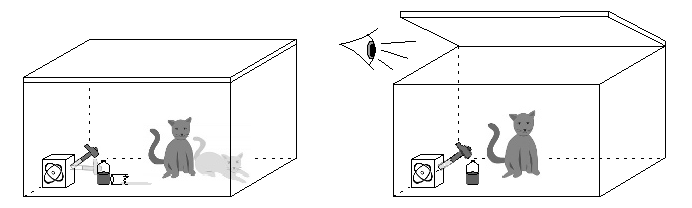
\includegraphics[width=.96\linewidth]{figures/ch01_fig01.pdf}
\caption{Schrödingerの猫の逆説の模式図。左：量子力学の法則は、不安定な原子、ハンマー、毒、猫を含む複合系を、古典的には互いに両立しない二つの状態の重ね合わせにする。一方には生きた猫が、他方には死んだ猫が含まれる。右：量子力学の標準的解釈によれば、観測者が箱を開けて猫を見ると、重ね合わせはその二成分のいずれか（ここでは「生きている」成分）へと「収縮」する。しかし、これは箱が開かれる前の猫の状態という問いを先送りする。}
\end{figure}

\hypertarget{srcpage:3}{}\label{srcpage:3}逆説の第二の部分は、外部の観測者の登場によって成立する。観測者が箱を開けると、標準量子論は、その観測者が重ね合わせを二つの成分状態の一方へと「収縮」させると予測する。こうして観測者は、経験と一致して、この二状態のいずれか一方しか知覚しないことが保証される。したがって観測者は、不運な動物をただ見るだけで、猫の運命を突然決めてしまうように思われる。そこで逆説は、次の単純な問いになる。観測者が箱を開ける前、猫はどのような状態だったのか。生きていたのか、死んでいたのか、生きても死んでもいたのか、それともそのいずれでもなかったのか。そもそもこの問いに意味はあるのか。同様の趣旨で、Einsteinは皮肉を込めてこう尋ねたと伝えられている\cite{ref003}。誰も見ていないときにも月はそこにあるのだろうか。

ある意味では、量子系が「量子性」を失って実効的に古典的になるうえで、系の開放性が重要であるという認識の種は、猫の逆説のような例の中にすでにまかれている。猫が「古典的」であること（すなわち、生きているか死んでいるかのいずれかであること）を保証するには、観測者は文字どおり箱を開けて猫を見る必要があるように思われる。

しかし、Schrödingerの設定では、観測者の役割は単に量子力学の収縮（または「射影」）公準から導かれる。観測者は、猫と相互作用する巨視的な量子系として物理的に扱われていない。さらに、猫の設定の残りの部分には、孤立系という仮定が暗黙のうちに置かれている。Schrödingerは、猫が毒と相互作用すると考えた。その毒は、毒入りの小瓶を割るハンマーを介して不安定な原子と結び付き、それによって微視的領域と巨視的領域の結合が成立する。しかし、それ以外の点では、猫は宇宙の残りの部分から孤立しているとされた。

Schrödingerが猫の逆説を提示した1930年代には、それは単なるGedankenexperiment、すなわち思考実験と考えられていた。当時、干渉効果のような量子現象は微視的領域でしか観測されていなかった。そのため、経験する巨視的世界の記述には量子力学が不要だというだけでなく、量子力学をこの領域から完全に排除すべきだとも論じられた。後者の立場の一例が、微視的な「量子」領域と巨視的な「古典」領域との基本的な二元性を仮定する、量子力学のCopenhagen解釈である。

今日では、私たちの見方は劇的に変わった。一方では、微視的領域をはるかに超えて量子効果が実験室で観測されている。研究者たちは、互いに逆向きに流れるマイクロアンペアの電流の重ね合わせや、数十個の炭素原子からなる重い分子の干渉縞など、中間的および巨視的なスケールの「Schrödingerの子猫」を作り出した（第6章参照）。

他方では、過去およそ30年ほどのあいだに、孤立系の仮定こそが、量子から古典への移行を理解するうえでの決定的な障害だったことが、徐々に認識された。この仮定は、先に述べたように、古典物理学では非常に実り豊かであり、量子物理学へそのまま引き継がれたものであった。量子系の開放性、すなわち環境との相互作用は、量子系が（したがって、量子力学が普遍的な物理理論であると仮定すれば、すべての系が）いかにして実効的に古典的になるかを説明するうえで不可欠であると認識された。スケールを大きくすると、系の「量子性」がどのように視野から消えていくのか。そして最後には、猫は生きているか死んでいるかのいずれかであり、こうした古典的に異なる二性質の重ね合わせとしては決して観測されない、私たちの経験世界へどのように至るのか、ということである。

\hypertarget{srcpage:4}{}\label{srcpage:4}基礎にある量子的領域から古典世界が現れるうえで環境との相互作用が重要であることが、これほど長く見過ごされてきたのはなぜだろうか。考えられる一つの理由はすでに述べた。物理学とは（理想化された）孤立系を扱うものだという、深く根付いた考えである。この問題に関連して、もう一つ重要な理由を見いだせる。孤立系という概念がもともと考え出された古典物理学では、状態は局所的なのである。

例として、液体に浸された小さな花粉粒を考えよう。液体の分子との衝突により、この粒子は不規則なジグザグの経路を動くことがある（よく知られたBrown運動という効果である）。このように、環境は粒子の運動を乱す。すなわち、古典的な「雑音」として働く。それでも、液体の存在下であっても、花粉粒がつねに「個体性」を保つことは明らかである。言い換えれば、粒子のすべての物理的性質は、つねにその粒子自体の内部に保持されている。したがって、液体を取り除くことを想像すれば、その後にも以前と同じ粒子が見つかると期待する。

この状態の局所性という概念は、深く根付いている。実際、あまりに深く根付いているので、私たちはそれを当然と考える。量子論の不可解な特徴に接したことのない人が、この概念を疑うことはまずないだろう。実際、状態の局所性は、孤立系という理想化を物理的に正当化する。この描像では、系を周囲から孤立させても、環境雑音の効果（すなわち、環境による系の擾乱）が減るだけで、系の実際の「本性」は変わらない。そのため、孤立系という見方が長いあいだ無害とみなされてきた理由は、容易に理解できるかもしれない。

量子力学は、状態の局所性についての考えを根本的に再検討することを私たちに迫った。量子論においても相互作用は依然として局所的である（すなわち、量子力学はなお局所的な理論である）が、これらの局所的相互作用によって生成されうる状態は、明確に非局所的である。鍵となる概念は量子もつれである。そこでは、空間的に大きく隔たっていてもよい二つの系が、各系それぞれの二つの別々の量子状態へと、いわば「分解」できない量子状態で記述される（図1.2参照）。もつれた状態には、二つの系のあいだの量子的相関が含まれる。\hypertarget{srcpage:5}{}\label{srcpage:5}このような相関はしばしば、個々の部分系のどちらにも存在しない、複合系にとってまったく新しい物理的性質を担っている。これらの部分系は個体性を失った、と言うことができる。すなわち、物理的性質は少なくとも部分的には非局所的な量子的相関の中に保持されるようになり、そのため片方の部分系だけに帰属させられなくなるのである。大まかにいえば、量子もつれは、量子力学的な全体が部分の総和とは異なる状況を表すと結論できる。

\begin{figure}[htbp]\centering
\begin{tikzpicture}[>=stealth,scale=.9]
\draw (0,2) rectangle (2.4,3.4);\node at (1.2,3.05){系$\mathcal A$};\node at (1.2,2.5){$\psi_{\mathcal A}$};
\draw (0,-.6) rectangle (2.4,.8);\node at (1.2,.45){系$\mathcal B$};\node at (1.2,-.1){$\psi_{\mathcal B}$};
\draw[<->] (1.2,.8)--(1.05,1.05)--(1.35,1.3)--(1.05,1.55)--(1.2,2);
\draw[->,thick] (2.9,1.4)--(4.0,1.4);
\draw (4.5,-1) rectangle (7.4,3.8);
\draw[dotted] (4.9,2) rectangle (7,3.4);\node at (5.95,2.7){系$\mathcal A$};
\draw[dotted] (4.9,-.6) rectangle (7,.8);\node at (5.95,.1){系$\mathcal B$};\node at (5.95,1.4){$\psi_{\mathcal{AB}}$};
\end{tikzpicture}
\caption{量子もつれの原理の模式図。初めはそれぞれの量子状態$\psi_{\mathcal A}$および$\psi_{\mathcal B}$によって記述される二つの系$\mathcal A$と$\mathcal B$を考える。この二つの系がある仕方で相互作用すると、このような個々の量子状態ではもはや記述できなくなる。二つの系は互いにもつれ、複合系$\mathcal{AB}$にだけ量子状態$\psi_{\mathcal{AB}}$を割り当てられる。}
\end{figure}

したがって量子的描像では、系と環境のあいだの（局所的な）相互作用は、古典物理学におけるよりもはるかに大きな役割を果たしうる。通常、その相互作用は両者のもつれを生み、それによって、系のレベルで観測できる事柄を根本的に変えるという意味で、対象自体の本性を変える。

このように量子的な状況では、環境との相互作用は、対象の系の物理を適切に記述するために最小限に抑えるべき単なる「擾乱」でも、その相互作用が十分「弱い」なら単に無視できるものでも、もはやない（後者の例は、ビリヤード球のNewton力学的軌道に対する空気分子の影響である）。むしろ環境との結合が、系の観測可能な物理的性質を定める。同時に、系の「量子性」の尺度である量子コヒーレンスは、もつれた系と環境の状態へと非局在化され、実効的に観測から失われる。この過程は、実際上は通常不可逆であり、私たちの経験する古典世界が基礎にある量子的基盤からどう現れるかを説明するうえで、重要な要素になる。（これらの考えは次章で、はるかに正確なものにする。）

\hypertarget{srcpage:6}{}\label{srcpage:6}したがって、環境との相互作用（ゆえに量子もつれ）が量子系にもたらす主要な帰結は、互いに密接に関係する次の二つである。
\begin{enumerate}
\item 干渉効果のような量子現象の源である量子コヒーレンスが、系から実効的かつ不可逆的に消失する。
\item 系の観測可能な性質が動的に「定義」される。すなわち、系に対して、頑健な優先状態（あるいは形式的には可観測量）の集合が選ばれる。
\end{enumerate}

これらの帰結は、環境誘起デコヒーレンス、略してデコヒーレンスという名称のもとにまとめられており、それが本書の主題である。「デコヒーレンス」という用語の由来は、上の第一の帰結から明らかであろう。第二の帰結は、文献ではときに、環境誘起超選択という独自の名称で呼ばれる。この用語は、許される重ね合わせの空間を（通常は公理的に）制限し、すなわち特定の可観測量の存在を禁じる、物理学のいわゆる超選択則との類似に由来する。同様に、環境との相互作用は、与えられた量子系で実際に観測できる物理量を、あらゆる実用上の目的に対して強く制限する。これらの制約は、系と環境の相互作用から動的に生じ、日常世界で私たちが位置や運動量といった少数の「古典的」で頑健な量しか観測しない理由を説明する。

読者は、それでもなお、1930年代に量子力学の主要な形式体系が完成した時点から、環境との相互作用とデコヒーレンスが量子から古典への移行にとって重要であることを示した、1970年代および1980年代の最初の画期的な研究\cite{ref004,ref005,ref006,ref007,ref008,ref009}まで、これほど長い時間が経過した理由を疑問に思うかもしれない。1930年代には、Schrödingerの猫に典型的に示される、量子から古典への移行の問題も認識されていた。結局のところ、量子もつれは、確立された局所性の概念に対する直観に反した帰結も含めて、すでによく知られていた。1935年には、Einstein、Podolsky、Rosen（EPR）\cite{ref010}が重要な論文を著し、もつれが含意する量子世界の不可解な「全体論的」かつ非局所的な性格を指摘していた。それならなぜ、量子的領域から古典世界が現れる仕組みの説明に、環境との相互作用ともつれが決定的に重要であると研究者が気付くまで、さらに40年を要したのだろうか。

この問いに対しては、少なくとも二つの相補的な答えが考えられる。第一に、Schrödingerが（微視的な系と巨視的な系をもつれさせることに基づく）猫の逆説を提示した後でさえ、もつれは、かなり長いあいだ、むしろ珍しい状況に見えていたかもしれない。それはしばしば、精巧な装置を用いて実験室で作り出す必要のある現象であって、それ以外の領域、とりわけ私たちの経験する巨視的世界では、重要な役割を果たさないと考えられていた。

\hypertarget{srcpage:7}{}\label{srcpage:7}この評価は誤りであることが判明した。実際には、もつれはとりわけ巨視的領域で至るところに存在することが示されている。さらに、しばしば関心は利用可能なもつれ、すなわち特定の「量子プロトコル」（たとえば量子暗号）を実行するために、制御しながら操作して利用できる量子的相関に向けられた。この立場は、量子情報と量子計算の研究者のあいだでよく聞かれる、「資源としてのもつれ」という標語に明瞭に表れている。もつれは確かにそのように利用できるが、通常は、制御されておらず、そのため「利用できない」環境とのもつれとして現れる。

古典性の出現に対する環境との相互作用ともつれの重要性が比較的遅く発見された第二の理由は、ごくわずかな環境さえ量子から古典への移行を引き起こすうえできわめて有効であることが、長いあいだ認識されなかった点に求められるかもしれない。たとえば古典物理学では、入射光（すなわち光子）が巨視的物体の運動状態に及ぼす影響を、ほとんどどのような場合にも無視してよい（図1.3参照）。光子から物体に渡される運動量は、通常、物体の運動を乱すのに必要な量に比べて無視できるほど小さい。さらに、入射光子はしばしば等方的に分布するので、正味の運動量移行は平均するとゼロになる。

しかし、古典的描像から量子的描像に移ると、状況は完全に変わる（再び図1.3参照）。今度は、光子と物体の散乱相互作用によって両者のあいだに量子的相関が形成され、それがコヒーレンスを物体から「運び去る」。\hypertarget{srcpage:8}{}\label{srcpage:8}その結果、物体のレベルで観測できる「量子性」の度合いは小さくなる（これらのかなり比喩的な用語は、後で改めて正確にする）。このもつれの生成には、物体に渡される運動量の大きさはまったく関係しない。実際、個々の光子から系への運動量移行がまったくないと仮定してもよい。したがって、光子は物体の運動状態に古典的な擾乱を引き起こす必要がなく、それにもかかわらず物体に強いデコヒーレンス効果を及ぼす。デコヒーレンスは、古典的な散逸過程（すなわち系からのエネルギー損失）と同時に起こることはあるが、散逸とは別の、古典物理学に対応物のない純粋に量子力学的な効果である。

\begin{figure}[htbp]\centering
\begin{tikzpicture}[>=stealth,scale=.85]
\node at (1.5,3.4){古典的な場合};\node at (7,3.4){量子的な場合};
\filldraw[fill=gray] (1.5,1.5) circle (.62);\draw[->,thick] (.2,.1)--(3,3);
\foreach \a in {0,35,75,110,150,190,225,265,300,330}{\draw[->,dashed] ({1.5+1.4*cos(\a)},{1.5+1.4*sin(\a)})--({1.5+.72*cos(\a)},{1.5+.72*sin(\a)});}
\filldraw[fill=gray!25] (4.6,-.25) rectangle (9.4,3);
\filldraw[fill=gray] (7,1.35) circle (.62);
\foreach \a in {25,75,140,190,250,310}{\draw[->] ({7+.6*cos(\a)},{1.35+.6*sin(\a)})--({7+1.4*cos(\a)},{1.35+1.4*sin(\a)});}
\node[font=\scriptsize] at (5.7,2.5){コヒーレンス};\node[font=\scriptsize] at (8.4,2.5){コヒーレンス};\node[font=\scriptsize] at (5.5,1.15){コヒーレンス};\node[font=\scriptsize] at (7.8,0){コヒーレンス};\node at (7,-.65){$\psi_{\text{物体＋光子}}$};
\end{tikzpicture}
\caption{古典的な場合と量子的な場合で環境が系に及ぼす影響の違いを、全方向から入射する光（光子）の中に置かれた巨視的物体を例に示す。左：古典的な場合には、環境が系と強く相互作用していても、物体による光の散乱は物体の運動を変えない。右：量子的な場合には、相互作用によって物体と光子のもつれた状態$\psi_{\text{物体＋光子}}$が生じる。コヒーレンスは物体から非局在化し、干渉縞のような量子効果は系のレベルで観測できなくなる。}
\end{figure}

本書で見るように、環境粒子の散乱によって巨視的物体に生じるデコヒーレンスは、驚くほど強く、速い。物体を、十分に離れた二つの異なる位置のコヒーレントな重ね合わせのような非古典的量子状態に準備しようとしたとする（大ざっぱにいえば、物体が「同時に二か所にある」状況と呼べる）。物体で散乱される光子との環境もつれは、ごく短い、1秒のわずかな端数のあいだに、重ね合わせの二成分間のコヒーレンスを完全に非局在化させる。このように、物体のレベルでの観測という実用上のあらゆる目的に対して、物体の振る舞いはほとんどすべての場合、私たちが時間的に分解できるよりもはるかに速く、実効的に古典的になる。さらに驚くべきことに、これには入射光という環境さえ必要ない。至るところにある熱放射だけでも完全に十分であるばかりか、宇宙に満ちたBig Bangの名残である宇宙背景放射でさえ、巨視的物体に急速なデコヒーレンスをもたらす（第3章参照）。

これは、デコヒーレンスがきわめて有効であるだけでなく、実際上ほとんど逃れられないことを示す。そしてそのことは、日常経験の世界で、Schrödingerの猫の重ね合わせのような「奇妙な」量子効果を観測するのが、なぜこれほど難しいのかを説明する。さらに、ここで本章の冒頭の議論へ戻れば、量子力学がこれほど長いあいだ、通常はかなりよく孤立した微視的系の文脈で論じられてきた理由をも示しているかもしれない。系が環境からきわめてよく遮蔽されていなければ（巨視的物体では実際上ほとんど不可能である）、関心のある特異な量子効果の観測は、通常、デコヒーレンスによって事実上不可能なほど困難になる。

古典世界の現れを、巨視的領域にまで拡張した量子力学の予測とどう両立させるか、あるいはそこからどう導くかという問いは、量子力学の最も大きな基礎的問題の一つである。この問いが（少なくとも部分的な）答えを得たのは、あらかじめ抱いていた古典的概念を量子力学に押し付けて、巨視的領域に対する量子力学の「奇妙な」含意を単に追い払うことによってではなく、\hypertarget{srcpage:9}{}\label{srcpage:9}量子力学自体の内部からであったというのは、ほとんど皮肉である。結局、当初はSchrödingerの猫やEPRのような「逆説」をもたらすだけだと考えられていた、明確に量子力学的なもつれという現象こそが、最後には系の観測される古典的振る舞いを強制するのである。

したがって、私たちに深く根付いた「古典性」という概念は、創発的な概念として理解できる。それは量子力学の特異な特徴によって否定されるものではなく、むしろ正当化されるものなのである。すべての古典的概念を、環境との相互作用とデコヒーレンスの実効的な帰結としてどの程度まで導けるのか、したがって物理理論における基本的役割をこれらの概念からどの程度まで取り除けるのかは、確かに未解決の問いであり、量子力学の基礎に関心をもつ研究者のあいだで活発な議論を生み続けている。本書では、量子論が普遍的に妥当であると仮定し（これに反する説得力のある実験的証拠は存在しない）、この理論の内部から古典性を説明しようとするならば（これはきわめて望ましい目標である）、デコヒーレンスが、私たちの周囲の古典世界の現れに対して「望みうるかぎり最良の」説明を与えることを示す。

デコヒーレンスが引き起こす実効的な古典性の背後の「究極の物理的実在」に関連して、未解決の概念的な問いがいくつか存在するのは確かである。これらの問いの具体的な形は、量子力学に対する解釈上の立場によって変わる傾向がある。しかし、古典性の出現を完全に量子力学から導くならば、この種の問いは避けられない。結局、重ね合わせ状態や非局所的な量子的相関など、量子論のすべての「奇妙な」非古典的現象は、ある大域的なレベルでは存続しなければならない。それらは公準によって追い払われたのではなく、むしろ私たちの経験する古典世界を導くために使われたからである。

こうした解釈上の問題にあまり深入りする前に（本書のさまざまな箇所、とりわけ第8章で再び取り上げる）、過去数年間にデコヒーレンスが多くの実験で広範に研究されてきたことを強調しておこう（第6章参照）。さまざまな実験で、対象の系と環境の相互作用を制御し、デコヒーレンスの漸進的な作用と、それに伴う量子的領域から古典的領域への段階的な移行を観測することが可能になった。たとえば、回折格子を通過した大きなフラーレン分子による量子干渉縞は、周囲の気体分子の密度、したがってフラーレンと環境粒子の散乱頻度を増やすにつれて、徐々に減衰することが観測された。このようなデコヒーレンス過程の特徴的な時間は高い精度で測定され、理論予測と見事に一致することがわかった。これらの実験が非常に注目すべきなのは、異なる定量的な程度のデコヒーレンスを調べられるからである。すでに存在する、身の回りの完全に古典的な巨視的世界の現れを、きわめて有効で高速なデコヒーレンスの作用に単に帰属させるだけでなく、環境との連続的な相互作用が、中間的および巨視的な領域の量子現象を観測する能力をどのように徐々に損なうかを、今や直接測定できるのである。

\hypertarget{srcpage:10}{}\label{srcpage:10}量子力学を実際に用いる多くの人々、とくに物理学の実験分野と量子計算分野の研究者は、現在、デコヒーレンスに対して非常に実用的な態度を取っている。たとえばデコヒーレンスは、装置の実験的実現を妨げる「量子雑音」の一種としてしばしば捉えられる（たとえば量子計算に「誤り」を持ち込むことによって）。ますます現実的なデコヒーレンス模型が開発され、その予測は実験で観測されたデコヒーレンス現象と比較されてきた。研究に携わる物理学者のあらゆる実用上の目的にとって、デコヒーレンスは、量子から古典への移行を定性的にも定量的にも記述する、完全かつ自己完結した枠組みを与える。他方、デコヒーレンスが「私たちの経験する古典世界」のような哲学的意味合いの濃い概念に適用される以上、概念的に興味深い問いをいくつか生むことは、ほとんど意外ではない。

デコヒーレンスは、系と環境の相互作用に量子力学の標準的な形式体系を適用した単なる帰結である。したがって、それは量子力学自体とは別の外来の理論でも、含めるか無視するかを自由に選べるものでもない。デコヒーレンスは自然界に遍在する効果であり、物理系の現実的な記述に到達するには、広範で魅力的なその帰結を考慮しなければならない。

過去数年間に、デコヒーレンスに関する文献の量は膨大なものになった。デコヒーレンスの主要な考え方と概念を導入した、画期的な初期論文を調べたい読者のために、ここで主要文献のいくつかを簡単に概観しよう（デコヒーレンス研究の発展に関するさらに詳しい歴史的考察は文献\cite{ref011}参照）。後に「デコヒーレンス」として知られるようになるものについての最初の論文は、University of HeidelbergのH. Dieter Zehによって執筆され、1970年に\textit{Foundations of Physics}に発表された\cite{ref004}。そこでZehは、現実的な巨視的量子系は決して閉じておらず、環境と強く相互作用することを指摘した。したがって、Schrödinger方程式が普遍的に妥当だと仮定すれば、そのような系は通常、環境と量子的に相関した状態にあり、そのことが波動関数の成分の「動的な分離」と、系自体の力学をSchrödinger方程式で記述できないことをもたらす。Zehは、これによって巨視的系の量子状態の観測される脆さと、超選択則の出現を説明できるかもしれないと提案した。続く論文\cite{ref006}では、彼とOlaf Küblerがもつれの力学を調べ、コヒーレント状態の動的な頑健さを強調した。しかし、「デコヒーレンス」という用語が導入されたのは1980年代末になってからであった。実際、1970年代の大半を通じて、デコヒーレンスはまったくといってよいほど関心を集めなかった（Zehは最近、これを「デコヒーレンスの暗黒時代」と呼んだ\cite{ref011}）。

\hypertarget{srcpage:11}{}\label{srcpage:11}デコヒーレンス研究の発展が一つの画期に達したのは、1981--82年に、Wojciech Zurek（1981年にはJohn Wheelerのポスドクであり、1982年にはCaltechのTolman Fellowであった）が、デコヒーレンスについての方向を定める二つの論文を\textit{Physical Review D}に発表したときである\cite{ref008,ref009}。Zurekは、デコヒーレンスと量子から古典への移行の問題で中心的な、いわゆる「優先基底問題」（次章で論じる）の重要性を明確に指摘した。彼は、デコヒーレンス研究の礎となる環境誘起超選択という概念を発展させ、環境によって超選択される優先状態（彼が「ポインター状態」と呼んだもの）を決定するための、厳密な枠組みを定義した。優先状態を選ぶための主要な基準として、量子的相関の保存が重要であることを強調した。また、環境誘起超選択が優先基底問題を実効的に解消する仕組みと、日常世界で位置が至るところで優先される量として観測される事実を説明する仕組みを示した。Zurekの研究はデコヒーレンスに光を当て始め、その「暗黒時代」の終わりの始まりとなった。デコヒーレンス研究の発展へのもう一つの重要な貢献は1984年に行われた。Zurekは、典型的なデコヒーレンスの時間尺度を評価できる、非常に一般的で単純な（そして今なお広く用いられる）表式を導いたのである\cite{ref012}。この研究は当時、一連の講演で紹介され、Los Alamosの報告書にも記述されたが、（1984年の会議の議事録の一部として）「公式に」出版されたのは1986年になってからだった。

1985年には、（Zehの学生だった）Erich JoosとZehが、環境粒子の散乱によって引き起こされるデコヒーレンスの詳細な模型を示す重要な論文を、\textit{Zeitschrift für Physik}に共著で発表した\cite{ref007}。この論文には、異なる種類の環境の中に置かれた、さまざまな大きさと物理的性質をもつ物体について、デコヒーレンスの時間尺度を初めて明示的に数値評価した結果も含まれていた。Zurekの論文とJoosおよびZehの論文は、ともに、デコヒーレンスが、とりわけ巨視的スケールでは、きわめて高速かつ効率的な過程であることを明らかにした。

1991年に、Zurekの\textit{Physics Today}の論文\cite{ref013}が、デコヒーレンスをより広い読者に紹介した。この論文はデコヒーレンスが物理学の主要な一分野として確立されることを助け、デコヒーレンスはついに、物理学者、物質科学者、哲学者から広い関心を集め始めた。（Joosはかつて、デコヒーレンスが量子力学の基礎的問題に対してもつ含意がこれほど長く見過ごされていたのは「歴史的な偶然」だったと述べた\cite[p.~13]{ref014}。）環境の役割をめぐる継続的な研究は、新しい発展を生み続けている。その例は、いわゆる「量子Darwin主義」、「証人としての環境」という研究構想、量子もつれと確率の関係であり、いずれもZurekと共同研究者が始め、現在取り組んでいる研究課題である。それらは、私たちが慣れ親しんだ古典的な日常世界の量子的起源について、いっそう完全な描像を与えている。\hypertarget{srcpage:12}{}\label{srcpage:12}高まり続ける量子計算への関心は、デコヒーレンス研究をさらに促進し、デコヒーレンス過程を積極的に制御し、遮蔽し、軽減するための、新しい理論的・実験的な道を開いた。こうして、さまざまな側面、含意、応用をもつデコヒーレンスは、現在もなお完全な解明にはほど遠い。今後も多くの刺激的な発展を目にし続けることは確実である。

本書に加えて、関心のある読者は、PazとZurekの論文\cite{ref015}、Zurekの論文\cite{ref016}、Joosらの著書\cite{ref017}に、デコヒーレンス研究の総説を見いだせる。より専門的なBreuerとPetruccioneの著書\cite{ref018}にも、デコヒーレンスに関する内容がある。次章では、デコヒーレンスの基礎をなし、この予備的な議論ではいささか大まかに導入してきた、さまざまな概念と考え方を、概念的にも形式的にも、より正確にしていく。

\clearpage
\setcounter{section}{1}
\setcounter{footnote}{0}
% 原文 pp.13--19、およびp.20冒頭の継続段落。本文を段落単位で照合。
\sectionlink{デコヒーレンスの基本的な形式と解釈}
% 原文 p.13
\hypertarget{srcpage:13}{}\label{srcpage:13}
本章の前半では、デコヒーレンスの研究計画を支える量子力学の形式と解釈のいくつかを紹介する。まず量子状態を論じる（2.1節）。量子力学が古典物理学と異なる点の多くは、量子状態の概念と解釈を中心に整理できる。古典物理学では「系の状態」は、位置、運動量、温度などの物理量の値を列挙したものを意味するにすぎない。量子物理学では、系は抽象的な状態ベクトルによって記述され、一般にこれを観測される物理的性質と結び付けるには、量子測定という付加的な概念を必要とする。しかも、この概念はよくても曖昧にしか定義されていない。

続く2.2節では量子力学の重ね合わせ原理を論じる。抽象的な量子状態という概念が古典力学と量子力学の最初の重要な相違であったとすれば、重ね合わせ原理は両者の隔たりをさらに広げる。デコヒーレンスの大部分は量子的重ね合わせの問題を中心にしている。すなわち、自然界でどの重ね合わせを観測できるかを教える中心的な機構であり、重ね合わせ原理によって原理上は許される重ね合わせの大半が、実際には周囲の世界で見られない理由を説明する。

2.3節では、デコヒーレンスにとって重要な、もう一つの量子力学特有の概念、すなわち量子もつれを導入する。量子もつれは、量子計算などの技術的応用において量子力学の力を利用するための中心的な要素となっている。また、デコヒーレンスの基礎にある機構でもある。2.4節では、デコヒーレンスの形式的記述に重要な道具となる密度行列の形式と解釈を論じる。2.5節では量子力学の測定問題と、それに関連する量子から古典への移行の問題をやや詳しく紹介する。デコヒーレンスはこれらの問題と密接に関係し、本章および第8章で見るように、少なくとも部分的な解決を与える。

2.6節では二重スリット実験を例として、デコヒーレンスに不可欠な量子もつれの帰結、すなわち、ある系ともつれた相手に「どちらの経路を通ったか」という情報が符号化されることを論じる。この説明によって、系と環境の量子もつれを介した、環境による系の「監視」の帰結としてデコヒーレンスを理解する道筋が開かれる。

% 原文 p.14
\hypertarget{srcpage:14}{}\label{srcpage:14}
続く2.7、2.8、2.9節では、この環境による監視の三つの主要な帰結を詳しく論じる。すなわち、系の水準での干渉効果の抑制、環境との量子もつれに最も影響されにくい準古典的な優先状態の選択、そして、これらの優先状態に関する情報が環境内に頑健かつ冗長に符号化されることである。第1章ですでに指摘したように、狭義のデコヒーレンスはしばしば第一の帰結（干渉の減衰）のみを指し、第二の帰結（優先状態の選択）は「環境誘起超選択」という別の用語で呼ばれる。しかし両現象は起源を共有し、不可分に結び付いている。干渉の減衰は、干渉が抑制される対象となる特定の状態の集合について述べる必要があるからである。この広い見方では、「デコヒーレンスの研究計画」は、環境による監視の上述の三つの帰結をすべて含むものと考えるべきである。

2.10節では、具体的で単純なデコヒーレンス模型を通じてこれらの考えを検討する。残りの各節では、いくつかの重要な追加の話題を論じ、全体像を完成させる。デコヒーレンスと散逸（2.11節）、およびデコヒーレンスと古典的雑音（2.12節）の根本的な相違を強調する。2.13節ではデコヒーレンスが可逆となりうる例を述べ、関連する量子的「消去」の過程を分析する。2.14節では、デコヒーレンスの研究計画の重要な概念的問題である、宇宙を部分系に分解する問題を論じる。最後に2.15節では、さらにいくつかの形式的な道具、すなわちSchmidt分解定理（2.15.1節）、Wigner表示（2.15.2節）、非純粋状態の純粋化（2.15.3節）、およびKrausの演算子和形式（2.15.4節）を概説する。

\subsectionlink{量子状態の概念と解釈}
\subsubsectionlink{古典状態と量子状態}
古典物理学における物理系の「状態」という概念は、きわめて直観的である。通常、たとえば運動する物体の位置や運動量のような、関心のある測定可能な量に注目し、それらの量に数学的記号（「$x$」や「$p$」など）を割り当てる。すると、これらの記号に数値を与えるだけで物体の運動状態が指定される。言い換えれば、物体の物理的性質（したがって物理世界の実在物）と、理論におけるその形式的・数学的表現との間に一対一の対応が存在する。

% 原文 p.15
\hypertarget{srcpage:15}{}\label{srcpage:15}
もちろん古典物理学でも、ここで用いたNewton力学の例ほど容易には、この直接の対応が確立されない場合を考えることはできる。たとえば歴史的には、熱力学理論における温度の形式的定義を、物理的な温度概念の基礎となる分子過程に結び付けるのは、かなり難しいことが判明した。しかし通常は、他の物理量や現象を参照することによって、少なくともある水準ではこの同定の問題を解決できた。たとえば、集合的な熱力学変数を、物質の集まりに含まれる微視的構成要素の振る舞いに結び付けるのである。

20世紀初頭の量子論の登場によって、物理世界と理論内の数学的表現との、この単純な全単射的対応は突然終わりを迎えた。経験に現れる「客観的に存在する」物理的性質に直接対応する直観的な記号によって物理系の状態を記述する代わりに、量子力学で利用できるのは、同じく抽象的なHilbertベクトル空間内のベクトル（より一般には射線）として定義される、抽象的な量子状態だけである。

この抽象化に伴う概念的飛躍の大きさは、いくら強調しても足りない。実際、量子論の初期以来、数え切れない物理学者や哲学者が取り組んできた「量子力学の解釈」をめぐる議論は、その大部分がまさに、抽象的な量子状態を「外にある物理的実在」とどう関係付けるかという問いに根差している。

教科書的な量子力学によれば、経験上なじみのある物理量とのつながりは、間接的にのみ作られる。すなわち物理量の測定を通じてであり、その物理量、つまり観測可能量（「現実世界」の側）は、Hilbert空間内のHermite演算子（「形式的理論」の側）によって表される。通常用いられる収縮（または射影）公準によれば、測定は量子状態を、測定された観測可能量を表す演算子の固有状態の一つへと瞬間的に変化させる。それぞれの固有状態が得られる確率はBorn則\cite{ref019}で与えられる（原文35頁の脚注9を参照）。

測定される演算子の固有状態は、対応する物理量が測定で取りうる、互いに異なる確定した「値」を表す。したがって、これらの固有状態に結び付いた概念は、上で論じた古典物理学のものに似ている（もちろん、測定する観測可能量は、スピンの場合のように、明確に非古典的でありうる）。それゆえ測定は、ある程度まで、数学的形式と系の「客観的に存在する物理的性質」との一対一の対応、つまり古典物理学でなじみ深い概念への回帰を可能にする。

しかしここには、量子力学特有のもう一つの注意点が潜んでいる。多くの観測可能量が互いに両立しないため（形式的には、対応する演算子の非可換性によって表現される）、量子状態は一般に、きわめて少数の演算子観測可能量の同時固有状態でしかない。したがって量子系に帰属させられる確定した物理的性質の数は限られ、測定を追加すると一般に系の状態は変化する（「乱される」）。もちろん、まったくの幸運や事前知識によって、測定前の系の量子状態にたまたま一致する固有状態を持つ演算子観測可能量を測定する場合は別である。

% 原文 p.16
\hypertarget{srcpage:16}{}\label{srcpage:16}
量子状態のこの壊れやすさは、有名な複製不可能定理（7.4.1節）にも反映されている。この定理によれば、未知の量子状態を複製することは一般に不可能である\cite{ref020,ref021}。これを別の言い方で表すと、個々の系の未知の量子状態を、その系だけに対する測定によって一意に決定することは不可能である\cite{ref022,ref023,ref024,ref025,ref026}。

言うまでもなく、この状況は古典物理学と際立った対照をなす。古典物理学では、さらに別の物理量を、任意の順序でいくつでも測定することにより、系の物理的性質の「一覧」を拡張し、したがって状態をより完全に指定できる。さらに、多数の独立した観測者が、初めは系の状態についてまったく知らなくても、状態を乱す危険にさらされることなく、そのような測定を行い、結果について一致できる。もちろん、このように古典状態が客観的にあらかじめ存在することが、私たちの深く根付いた「古典的実在」の概念をもたらした。

以下では、曖昧さが生じる場合を除き、物理的観測可能量を表すHermite演算子を、より正確な「演算子観測可能量」という語の代わりに、単に「観測可能量」と呼ぶことが多い。それでも、形式的演算子と物理量との同一視は量子論に公理的に導入されるものであり、自明ではないことを念頭に置いてほしい。ただし、観測可能量の概念を創発的なものと見なし、量子状態の形式だけから導くこともできる。この見方はJohn Bellの「beable」の探究\cite{ref027}の精神に沿うものである（その例は文献\cite{ref017}の2.2節を参照）。物理量の測定を、過度に単純化して「演算子の測定」と記述することにより、このような演算子について素朴実在論に陥る危険は、すでに指摘されている\cite{ref028}。

\subsubsectionlink{量子状態の確率的性格}
前節で論じた量子状態の性質を踏まえ、これらの状態は、観測されるさまざまな「古典」状態への「可能性」だけを表すのだと、しばしば主張されてきた。しかし同時に、現在の知識によれば、量子状態は量子系の完全な記述を表すことを強調するのが重要である。すなわち、量子状態は、系の物理状態について言いうるすべてを包含している。それでも一般には、量子状態は、測定で具体的にどの結果が得られるかを教えず、可能なさまざまな結果の確率だけを教える。量子力学の、この一見内在的な確率的性格は、この理論を古典物理学から区別する中心的な特徴の一つである。実験では、この確率的側面は、まったく同じ量子状態に準備した系の集まりについて同じ物理量を測定すると、一般に異なる結果の集合が得られることとして現れる。

% 原文 p.17
\hypertarget{srcpage:17}{}\label{srcpage:17}
よく知られているように、Einsteinは生涯を通じて、自然のこの見かけ上内在的な偶然性を受け入れることに消極的だった\cite{ref029}。それは「神は宇宙でさいころを振らない」という有名な言葉に表れている。この不満は他の人々にも共有され、彼らは、量子状態だけでは系の物理状態を完全には指定できないという意味で、量子力学は完全な理論ではないと提案して、逃れる道を求めた。その場合、「同一に準備された系」の集団は、実際には物理的に同一な系の集まりを表していないことになる。集まりの各系は同じ量子状態で記述されても、それぞれの個々の系に対する、可能なすべての測定の結果を決める「完全な状態」は、集団の各要素で同一ではないというのである。

そのような手法は通常、隠れた変数理論と呼ばれる。これらは、系に対して行われる任意の測定の具体的結果を、その値が決定する「隠れた変数」を仮定して導入し、量子状態を補うことにより、根本的な水準で決定論を回復しようとする。したがって、量子状態と、関係する隠れた変数の値との組合せだけが、系の完全な物理状態を指定する。すべて同じ量子状態に準備された系の集団は、隠れた変数の異なる値の範囲によって記述されることになる。こうすれば、測定結果が異なることを完全に決定論的に説明できる。量子力学が私たちに確率的に見えるのは、隠れた変数の具体的な値を知る手段がないからにすぎない（それゆえ「隠れた」と呼ばれる）。したがって量子力学の確率は、純粋に認識論的なものになる。古典統計力学と同じく、確率は私たちの主観的な知識の不足を表すにすぎず、物理学の根本水準における客観的な非決定性を表すものではない。

しかし実際には、実験によって十分に確かめられた標準量子力学の予言に反しない、隠れた変数の手法を構築するのは、きわめて難しいことが判明している。最も有名なのは、John Bellが1964年の画期的な論文で提示した不等式であり、あらゆる局所的な隠れた変数理論はこれを満たすが、標準量子力学はこれを破る\cite{ref030}（後にBellがさらに洗練した説明\cite{ref027,ref031}も参照）。多数の実験がBellの不等式の明確な破れを示し、局所的な隠れた変数理論を、ほぼ決定的に排除した\footnote{実験結果の解釈には、ごくわずかで、しかも減少し続けてはいるが、なお余地が残っている。主な「抜け穴」は、検出効率が100\%に満たない不完全な検出器によるものである\cite{ref032}。もう一つの問題は「通信の抜け穴」と呼ばれるもので、現在ではWeihsらの実験\cite{ref033}によって閉じられたと一般に考えられている。}。これらの結果は、隠れた変数理論が機能するためには、高度に非局所的である必要を示している。そのような非局所的な隠れた変数理論の代表として、おそらく最も有名なのはde Broglie--Bohmの手法\cite{ref034,ref035,ref036,ref037}である（8.5節）。ここでは位置を隠れた変数に選び、系の各粒子は常に確定した位置を持つ。

% 原文 p.18
\hypertarget{srcpage:18}{}\label{srcpage:18}
さらにKochenとSpecker\cite{ref038}は、隠れた変数理論は必ず文脈依存でなければならないことを示した。すなわち、隠れた変数によって量子系に帰属させる物理量の具体的な値は、一般に測定の文脈、つまり最終的にその値をどのような仕方で測定するかに依存する。たとえば、その系について他のどの観測可能量を同時に測定するかによって、系は、ある観測可能量の異なる値を持つことになる。したがって文脈依存性は、そもそも隠れた変数の研究計画の動機となった中心的な考えを放棄するよう迫る。その考えとは、物理世界はそれに対して行うどんな測定からも独立であり、測定は、隠れた変数の値によって決まる、あらかじめ存在する物理量の値を単に明らかにするのだというものである。このように、いかなる隠れた変数の概念を仮定しても、提案どおりに機能するには、精緻で、高度に非局所的かつ文脈依存の機構が必要になることは明らかである。

\subsubsectionlink{量子状態の存在論的地位}
もう一つの論争は、量子状態の存在論的地位という問いを中心に展開してきた（簡潔で読みやすい歴史的概説は文献\cite{ref039}を参照）。量子力学の初期に、Schrödingerは実空間内の狭い波束を、実際の物理的粒子と同一視しようとした（第3章の冒頭）。この方策には二つの中心的な問題があった。第一に、初めに局在した波束は一般に、空間の広い領域へ急速に広がる傾向があり、定義上空間に局在する粒子という概念とは両立しない。第3章で見るように、この広がりは環境との相互作用によって実効的に抑制されるが、もちろん当時のSchrödingerはその過程を知らなかった。第二に、3次元実空間内の$N>1$個の粒子の量子状態を記述する波動関数は、$3N$次元のHilbert空間に存在し、もはや経験上なじみのある3次元空間内には存在しない。

その後、BornとPauliは別の手法を採り、量子状態は確率振幅を表す、すなわち、系に対して行いうるすべての測定の結果の確率を指定する、という有名な解釈を定式化した。そのうえで測定という行為が、これらの潜在的性質を動的に「現実化する」という根本的役割を果たすと仮定した。Wheeler\cite[p.~182]{ref040}（文献\cite{ref041}も参照）は、この見解を「どんな素過程［すなわち量子］現象も、それが記録された（観測された）現象になるまでは、現象ではない」と端的に表した。Heisenbergの「粒子の軌道は、私たちがそれを観測するという行為によって作られる」\footnote{ドイツ語の原文は「Die Bahn entsteht erst dadurch, daß wir sie beobachten.」である。}\cite[p.~185]{ref042}という言葉や、Bornに宛てたPauliの手紙にある、「観測の際に確定した位置$x_0$が現れること（中略）は、自然法則の外にある創造と見なされる」\footnote{原文は「Das Erscheinen eines bestimmten Ortes $x_0$ bei der Beobachtung (.\, .\, .) wird dann als außerhalb der Naturgesetze stehende Schöpfung aufgefaßt.」である。}\cite{ref043}という示唆にも、同様の考えが見られる。このように、広く受け入れられている波動関数のBorn--Pauli解釈は、量子状態が物理的実在を直接表すと見なす意味で、純粋に存在論的なものでもなく、私たちの主観的知識の不足だけを表すという意味で、単純に認識論的なものでもない。

% 原文 p.19
\hypertarget{srcpage:19}{}\label{srcpage:19}
しかしこの解釈は、「観測による現実化」の存在論的役割とは何か、そしてこの過程を力学的な言葉でどう物理的に説明するか、という根本問題を未解決のまま残す。この意味で、量子状態の解釈の問題は、測定の解釈の問題に置き換えられただけである。また、量子状態を測定された観測可能量の固有状態へと還元する波動関数の収縮を仮定しても、物理的性質の「現実化」の問題が解決されるわけではないことにも注意しよう。そのような収縮は、それ自体では状態の存在論的地位を変えない。したがって、収縮後の系の状態が、収縮前より「物理的に実在する」と見なすことはできない。

量子状態の「実在論的」解釈の対極をなすのは、先に述べた、量子状態の純粋に認識論的な見解である。この解釈では、量子状態は私たちの知識だけを記述し、系の客観的な物理状態を記述するものではないと見なす（その例は文献\cite{ref044}、およびBallentineの「集団解釈」\cite{ref045,ref046}を参照）。この見解を経験的に反証するのは明らかに難しいが、それは、私たちの観測、したがって「知識」の基礎にある物理的実在という根本問題を扱うことを頑なに拒んでいる。

本書では、量子状態ベクトル（たとえば標準的なDirac記法でケット$\lvert\psi\rangle$と表す）は、個々の系の物理状態の完全な記述を与えるという、広く受け入れられている考えを採用する。このような量子状態の「完全性」を反映して、これらは通常、純粋と呼ばれる。それに対し、いわゆる混合状態は、純粋状態の古典的な集団にすぎず、2.4.2節で論じる。私たちの目標は、まだ発見されていない「隠れた変数」をその場しのぎに導入したり、私たちの「知識」を量子形式が記述する根本的な対象と見なしたりする安易な道を採る代わりに、量子形式の内部から私たちの観測の性質を説明することである。

% 原文 pp.20--28、2.2節全体。
% 原文 p.20
\hypertarget{srcpage:20}{}\label{srcpage:20}
\subsectionlink{重ね合わせ原理}
重ね合わせ原理は量子力学の核心にあり、古典的な概念からの離脱を最も明瞭に示す特徴の一つである。形式的には、重ね合わせ原理はHilbert空間の線形性に根差している。量子状態はHilbert空間内のベクトルで表されるので、それらのベクトルの線形結合を作れる。重ね合わせ原理によれば、そのようなベクトルの線形結合は、再び新たな量子状態に対応する。これは、ケット$\lvert\psi_n\rangle$が量子状態の集合を表すなら、重ね合わせ
\begin{equation}\lvert\Psi\rangle=\sum_n c_n\lvert\psi_n\rangle\tag{2.1}\end{equation}
もまた、可能で、同じように許される量子状態に対応することを意味する。ここで$c_n$は任意の複素係数である。したがって重ね合わせ原理の平等性により、重ね合わせ状態$\lvert\Psi\rangle$は、成分状態$\lvert\psi_n\rangle$とまったく同様に、系の可能な物理状態に対応する。

たとえばスピン$1/2$の粒子を、二つの状態$\lvert0\rangle$（「上向きスピン」）または$\lvert1\rangle$（「下向きスピン」）の一方に準備できるとしよう。すると重ね合わせ原理は、$\lvert\Psi\rangle=(\lvert0\rangle+\lvert1\rangle)/\sqrt2$も同じように許される量子状態であり、したがって少なくとも原理上は、系をこの重ね合わせ状態にも準備できることを教える。

\subsubsectionlink{重ね合わせの解釈}
重ね合わせ原理がなぜこのような反直観的帰結を持つかを理解するには、量子力学的な重ね合わせを正しく解釈することが不可欠である。このような重ね合わせ状態は、単にその成分の古典的な集団を表すのではない（そのような集団はしばしば真正混合と呼ばれる\cite{ref047,ref048,ref049}）。すなわち、量子系が実際には成分状態$\lvert\psi_n\rangle$の一つだけにあるが、どれであるかを私たちが知らないという状況ではない（これを「素朴な集団解釈」と呼べる）。そうではなく、式(2.1)の各成分$\lvert\psi_n\rangle$が量子状態に同時に存在する。この状況を、それらの成分間にコヒーレンスが存在すると表現する。古典的な場合との違いを明確に強調するため、式(2.1)のような量子力学的重ね合わせは、しばしばコヒーレントな重ね合わせと呼ばれる。本書では、明示的に断らない限り、「重ね合わせ」は常に量子的な、すなわちコヒーレントな重ね合わせを意味する。そのような成分状態の重ね合わせは、個々の系の新しい物理状態を定義するのであって、成分状態の統計分布にすぎないものではない。

% 原文 p.21
\hypertarget{srcpage:21}{}\label{srcpage:21}
重ね合わせを、その成分状態の古典的な集団、すなわち、より根本的に確定された状態の集団と解釈することに反対する、一般的な議論を与えられる。証明は背理法による。状態$\lvert\psi_n\rangle$の重ね合わせ$\lvert\Psi\rangle=\sum_n c_n\lvert\psi_n\rangle$に、実際にそのような集団的見方を与えられると仮定しよう。すると測定によって追加の知識を得て、測定で得た結果と両立する状態からなる部分集団を取り出せる。時間発展はSchrödinger方程式
\begin{equation}i\frac{\mathrm d}{\mathrm dt}\lvert\Psi(t)\rangle=\hat H\lvert\Psi(t)\rangle\tag{2.2}\end{equation}
に従って完全に決定論的であったので、この特定の部分集団を時間を遡って追跡できることになる。その結果、系の初期状態、すなわち測定前の状態を、より完全に指定できる（この過程はしばしば「事後選択」と呼ばれる\cite{ref050}）。これは、その状態が、初めに準備した重ね合わせとは物理的に異なることを意味し、矛盾が生じる。

\subsubsectionlink{重ね合わせの実験的検証}
コヒーレンスの存在を実験で示し、それによって重ね合わせが、その成分状態の集団、すなわち真正混合と実際に異なることを、どう示せばよいだろうか。一般的な方法は二つある。重ね合わせ状態への直接の射影測定を繰り返すことと、干渉実験によって重ね合わせ内のすべての成分の存在を間接的に確認することである。いくつかの単純な例で、この二つの方法を説明しよう。

\paragraph{直接測定}
式(2.1)の形の重ね合わせ状態の存在を確認する最も直接的な方法は、同一に準備された系の集団の各要素について、観測可能量$\hat O=\lvert\Psi\rangle\langle\Psi\rvert$の射影測定を行うことである。各測定で1という結果が得られ、集団が十分大きければ、系は実際に重ね合わせ(2.1)に準備されていたに違いないと結論できる。

そのような測定を実現する装置の例は、Stern--Gerlach装置である（図2.1）。典型的なStern--Gerlach実験は次のように行われる。銀原子を炉で加熱し、コリメート用スリットと、$z$方向に不均一な磁場に通す（簡単のため、他の方向の磁場成分は無視する）。各銀原子は47個の電子を持ち、そのうち46個は球対称な電子雲に収まっている。したがって、47番目の電子のスピンだけが、原子全体の正味の磁気モーメントを与える。よって、比較的大きな質量を持ちながら、その磁気モーメントは単一電子のスピン磁気モーメントに等しい原子を扱うことになる。

% 原文 p.22
\hypertarget{srcpage:22}{}\label{srcpage:22}
\begin{figure}[htbp]\centering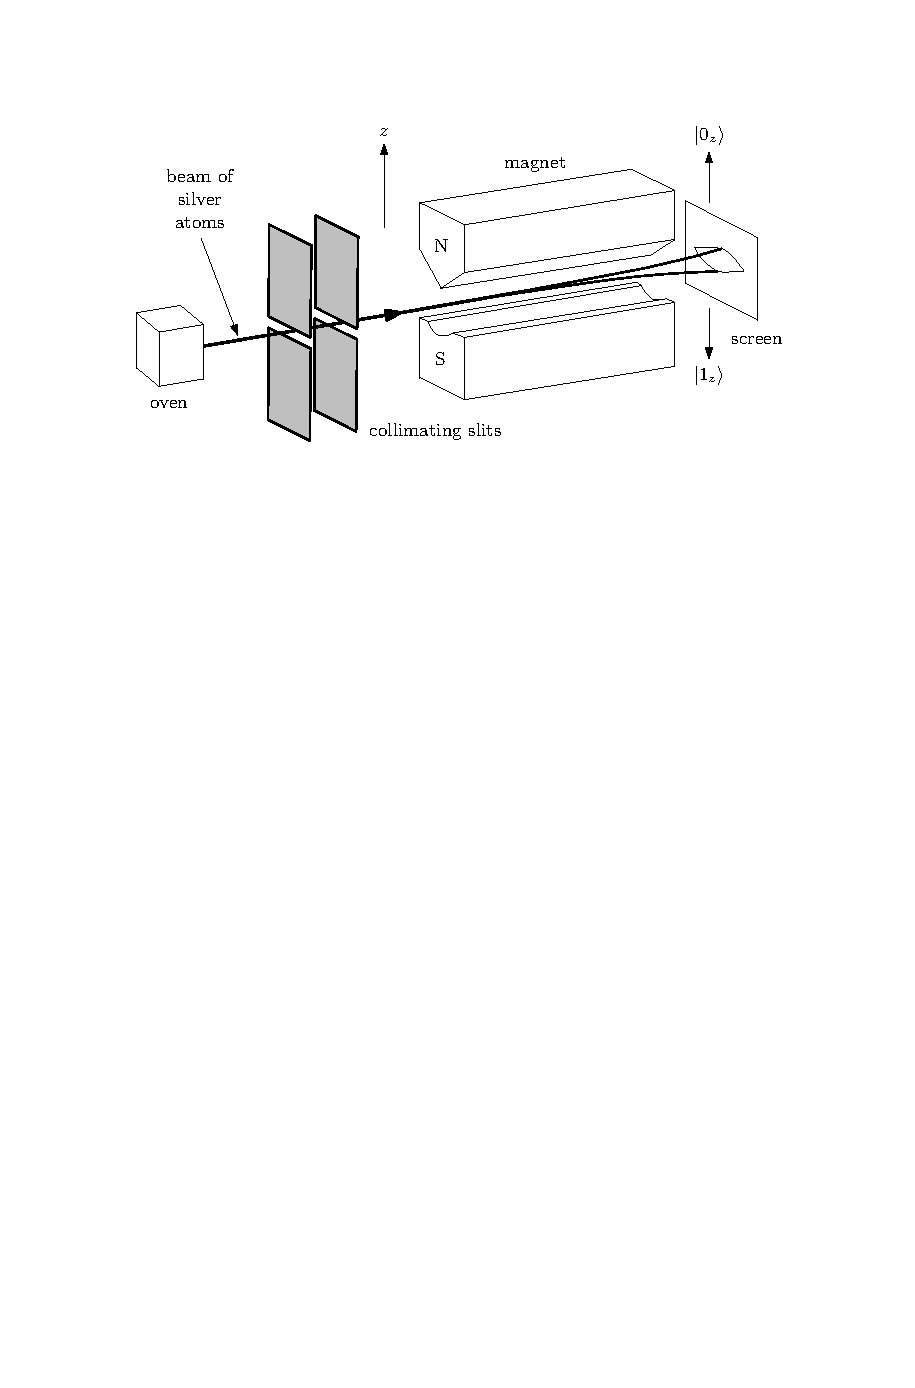
\includegraphics[width=.9\linewidth]{figures/ch02_fig01.pdf}\caption{Stern--Gerlach実験の模式図。単一電子のスピンに等しい磁気モーメントを持つ銀原子が炉から放出され、続いて$z$方向に不均一な磁場を通過する（不均一性は、たとえば磁石の磁極片の形によって生じる）。スピン状態に応じて、原子の経路は二つの可能な軌道に沿って曲げられ、$z$軸方向のスピンの量子化された値を示す。多くの原子が装置を通過すると、検出スクリーン上に二つの明瞭な帯が観測される。}\end{figure}

電子は$z$軸方向に、大きさが等しく向きが反対の二つのスピン値、すなわち「上向き」または「下向き」しか取れないので、銀原子の磁気モーメントには$\pm\mu_z$という二つの可能な値がある。銀原子が不均一な磁場を通過すると、磁気モーメントと磁場の相互作用によって$z$方向の力を受ける。この力は磁気モーメントの値に比例する。したがって、原子内の47番目の電子が$z$軸方向に上向きスピン状態にあるか、下向きスピン状態にあるかに応じて、銀原子の軌道は$+z$方向または$-z$方向に曲がる。これらの状態をそれぞれ$\lvert0_z\rangle$、$\lvert1_z\rangle$と書くことにし、これらはPauliの$z$スピン演算子$\hat\sigma_z$の固有状態である。原子ビームが検出スクリーンに当たると、原子が取りうる二つの異なる軌道に対応して、空間的に分離した二つの斑点が現れる。代わりに、一方の経路に粒子検出器を置けば、特定の原子がその経路を通ったかどうかが分かる。どちらの場合も、この装置は電子スピンの$z$成分の測定に対応する。

% 原文 p.23
\hypertarget{srcpage:23}{}\label{srcpage:23}
入射原子を、電子の$z$軸方向の「上向きスピン」に対応する量子状態、すなわち$z$スピン演算子$\hat\sigma_z$の固有状態$\lvert0_z\rangle$に準備するとしよう。予想どおり、スクリーン上の模様はこの準備を実験的に確認する。すべての原子がスクリーン上部に到達することが分かる。同時に、$\lvert0_z\rangle$は、直交する$x$軸方向の「上向きスピン」と「下向きスピン」の線形結合、$\lvert0_z\rangle=(\lvert0_x\rangle+\lvert1_x\rangle)/\sqrt2$とも等しく書けるので、この実験は、この重ね合わせが準備されたことを確認すると見なせる。もし重ね合わせが状態$\lvert0_x\rangle$と$\lvert1_x\rangle$の古典的な集団を表し、各電子が実際にはそのどちらか一方にあったなら、磁場の不均一性は$z$軸方向だけを向いていて原子ビームを分裂させないため、スクリーン中央に単一の斑点が現れるはずである。もちろん、実験ではそのような振る舞いは観測されない。逆に磁場の向きを90度回転させて$x$方向にすることもできる。この場合、初期状態$\lvert0_z\rangle$に準備したすべての原子について、ビームが50対50に分裂するのが観測される。

したがって重ね合わせ状態$\lvert0_z\rangle=(\lvert0_x\rangle+\lvert1_x\rangle)/\sqrt2$は、成分$\lvert0_x\rangle$と$\lvert1_x\rangle$が同時に存在する、個々の系の物理状態に対応する。それゆえ重ね合わせは、成分$\lvert0_x\rangle$と$\lvert1_x\rangle$の間の干渉縞という形でのみ現れるのではない（下記参照）。むしろ、Stern--Gerlach装置の磁場には、原子の軌道を「確実に予言」できるような向きが必ず存在する\cite{ref010,ref039}。

\paragraph{干渉実験}
Stern--Gerlach装置でのスピン測定の例は、かなり特殊な場合である。重ね合わせ状態に対応する射影観測可能量を直接測定するのは、通常きわめて難しいからである。代わりに、一般に利用できるのは、重ね合わせの成分に対応する特定の基底で測定を行う装置だけである。たとえば、Schrödingerの猫が生きているか死んでいるかを検出できる測定装置、つまり私たち自身の眼は存在する。これは$\{\lvert\text{「生」}\rangle,\lvert\text{「死」}\rangle\}$基底で測定する装置である。しかし、共役な基底$\{(\lvert\text{「生」}\rangle\pm\lvert\text{「死」}\rangle)/\sqrt2\}$で観測可能量を測定することに対応する、明白な手順は存在しない。もちろんこれこそが、Schrödingerの猫の重ね合わせ状態が、あれほど反直観的に見える理由である。普通、私たちにはそのような状態を直接観測する手段、すなわち測定装置、とりわけ人間の感覚がないのである。

この問題のより身近な例として、電子を個々に、すなわち一度に一個ずつ二重スリットに通す、有名な二重スリット実験を考えよう。スリットの位置では、電子は、それぞれスリット1、2を通ることに対応する成分$\lvert\psi_1\rangle$、$\lvert\psi_2\rangle$の重ね合わせ$\lvert\Psi\rangle=(\lvert\psi_1\rangle+\lvert\psi_2\rangle)/\sqrt2$で記述される。この重ね合わせの存在を直接確認するには、状態$\lvert\Psi\rangle$への射影測定が必要である。しかし、波動関数$\Psi(x)\equiv\langle x\vert\Psi\rangle$は、スリットに平行な各平面上で空間的に非局在化している一方、利用できる測定は、スリットの後方における粒子の位置測定だけである。したがって、射影観測可能量$\lvert\Psi\rangle\langle\Psi\rvert$を測定するには、二つの部分波$\psi_1(x)\equiv\langle x\vert\psi_1\rangle$と$\psi_2(x)\equiv\langle x\vert\psi_2\rangle$を、空間内の一点に正確に再集束させる必要がある。明らかに、これは実際上ほとんど不可能である。

% 原文 p.24
\hypertarget{srcpage:24}{}\label{srcpage:24}
このように、重ね合わせの成分状態を測定する手順しか使えない場合には、通常、重ね合わせ内の成分間の干渉効果を示す方法に頼る。基本的な考えは、重ね合わせ状態$\lvert\Psi\rangle=\sum_n c_n\lvert\psi_n\rangle$を定める展開係数$c_n$［式(2.1)］に、空間的または時間的変化を生じさせ、系が成分状態$\lvert\psi_n\rangle$の古典的な集団で記述される場合には、その変化が生じないように実験を設計することである。そのうえで、同一に準備した系の集団について、成分基底$\{\lvert\psi_n\rangle\}$で測定する。$\lvert c_n\rvert^2$は成分状態$\lvert\psi_n\rangle$を見いだす確率を指定するので、その確率が位置または時間に伴って変化することを観測すれば、系は実際に重ね合わせ状態$\lvert\Psi\rangle=\sum_n c_n\lvert\psi_n\rangle$に準備されていたと推論できる。重要な例を二つ挙げよう。

二重スリット実験では、遠方のスクリーン上の密度模様の空間的な変化、すなわちスクリーンの位置での粒子の位置空間密度分布$\varrho(x)$を測定する。よく知られた結果は干渉模様が得られるというものであり、それは、各電子がどちらか一方のスリットを通ると仮定した場合に予想される古典的模様とは、はっきり異なる（図2.2）。密度$\varrho(x)$は、成分状態$\psi_1(x)$と$\psi_2(x)$の古典的分布に対応する、各スリットを個別に通過する寄与の和を記述する波動関数の絶対値二乗の和、すなわち$\varrho(x)\propto\lvert\psi_1(x)\rvert^2+\lvert\psi_2(x)\rvert^2$ではなく、各波動関数の和の絶対値二乗で記述される。
% 原文 p.25
\hypertarget{srcpage:25}{}\label{srcpage:25}
\begin{equation}\begin{split}\varrho(x)&=\frac12\lvert\psi_1(x)+\psi_2(x)\rvert^2\\&=\frac12\lvert\psi_1(x)\rvert^2+\frac12\lvert\psi_2(x)\rvert^2+\operatorname{Re}\{\psi_1(x)\psi_2^*(x)\}.\end{split}\tag{2.3}\end{equation}
最後の項が、スクリーン上の特徴的な干渉模様の原因である。

\begin{figure}[htbp]\centering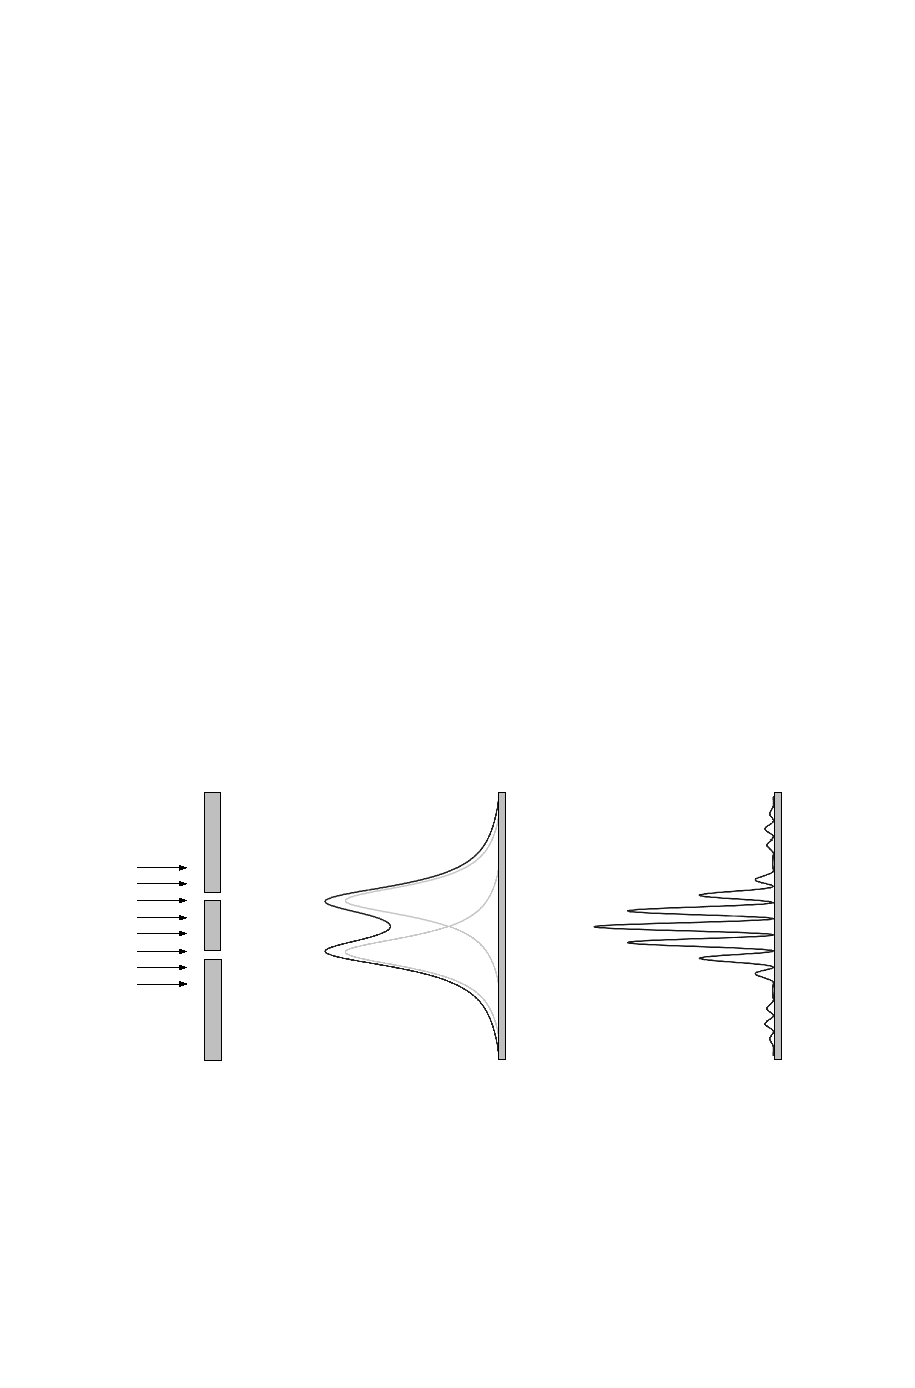
\includegraphics[width=.9\linewidth]{figures/ch02_fig02.pdf}\caption{粒子による二重スリット実験。左：粒子が二重スリットに入射する。中央：遠方の検出スクリーン上に得られる「古典的」密度模様。これは、各スリットからの寄与を単純に足し合わせたものに対応する。右：量子的な設定で得られる干渉模様（包絡線は回折によって変調されている）。}\end{figure}

この実験は、標準的な量子力学の形式の範囲内では\footnote{量子力学には、異なる見方を許す別の定式化も存在する。たとえばBohm力学では、すべての粒子の位置は常に確定しているとされる（8.5節）。したがって各粒子は、二つのスリットの一方を通る確定した軌道を進む。波動関数は依然として両スリットにわたって非局在化しているが、それは粒子が取りうるさまざまな経路を定めるだけである。}、個々の電子を、特定のスリットの通過を記述する一方の波動関数では記述できず、それらの波動関数の重ね合わせ$\Psi(x)=(\psi_1(x)+\psi_2(x))/\sqrt2$によってのみ記述できることを明瞭に示している。形式的には、この知見は、量子状態が実際の確率ではなく確率振幅を表すことによって説明される。つまり重ね合わせ状態は、確率ではなく確率振幅の線形結合を記述し、そのため重ね合わせに対応する確率分布(2.3)に干渉項が生じる。また、任意の時点で装置内に一個の粒子しか存在しないように二重スリット実験を行うことは十分に可能なので（6.2節）、干渉模様を異なる電子間の相互作用のせいにはできないことにも注意しよう。

干渉効果の観測により重ね合わせの存在を間接的に検証する、もう一つの例はRamsey干渉法\cite{ref051}である。今度は空間的変化ではなく時間的変化を用いる。Ramsey干渉法は、二準位系における量子的にコヒーレントなRabi振動の原理に直接基づいており、これは6.1.1節でより詳しく説明する。基底状態$\lvert g\rangle$と励起状態$\lvert e\rangle$で記述される二準位原子があり、その重ね合わせ状態$\lvert\psi\rangle=(\lvert g\rangle+\lvert e\rangle)/\sqrt2$の存在を示したいとしよう。しかし、実験では原子のエネルギー状態しか測定できず、$\{\lvert g\rangle,\lvert e\rangle\}$基底での測定だけが可能で、重ね合わせの直接の射影測定に必要となる共役基底$\{(\lvert g\rangle\pm\lvert e\rangle)/\sqrt2\}$では測定できない。

この場合も、干渉実験を行う方法によって目的を達成できる。まず、観測可能量$\hat O=\lvert g\rangle\langle g\rvert$の射影測定によって原子を基底状態$\lvert g\rangle$に準備する。次に、特定の持続時間のレーザーパルスを加えることによって（詳細は6.1.1節）、この状態をコヒーレントな重ね合わせ
% 原文 p.26
\hypertarget{srcpage:26}{}\label{srcpage:26}
\begin{equation}\lvert\Psi\rangle=\frac1{\sqrt2}(\lvert g\rangle-i\lvert e\rangle)\tag{2.4}\end{equation}
へと変換できる。その後、状態は自由に発展し続ける。
\begin{equation}\lvert\Psi\rangle=\frac1{\sqrt2}\bigl(\lvert g\rangle-ie^{-i\phi(t)}\lvert e\rangle\bigr).\tag{2.5}\end{equation}
ここで$\phi(t)$は、レーザーパルスの印加から時間$t$が経過したとき、ユニタリ発展によって生じる位相のずれである（$\lvert\Psi\rangle$の全体の位相因子は省略する）。式(2.5)は、いま実験で存在を確かめたい重ね合わせを表す。そのために、最初のパルスと同じ持続時間の二番目のレーザーパルスを加えると、状態(2.5)は
\begin{equation}\lvert\Psi\rangle=\sin\bigl(\phi(t)/2\bigr)\lvert g\rangle-\cos\bigl(\phi(t)/2\bigr)\lvert e\rangle\tag{2.6}\end{equation}
へと変わる。位相のずれ$\phi(t)$は、二つのレーザーパルスの間の時間$t$を変えることで調整できる。このようにして、重ね合わせの係数に時間的な変化を導入した。いま原子を$\{\lvert g\rangle,\lvert e\rangle\}$基底で測定すれば、$\phi(t)$の値に陽に依存する確率で、原子は基底状態または励起状態に見いだされる。

一方、レーザーパルスの間に、原子が重ね合わせ(2.5)ではなく、成分$\lvert g\rangle$、$\lvert e\rangle$の古典的な集団で記述されていたと仮定しよう。式(2.5)から明らかなように、パルス間の時間には、原子を基底状態と励起状態に見いだす確率は同じである。すなわち、重ね合わせ(2.5)に存在する位相のずれ$\phi(t)$は、式(2.5)から導かれる対応する古典的集団にはまったく無関係である。したがって、二つのパルスの印加の間に、原子が重ね合わせ(2.5)の代わりに成分状態の集団（真正な非コヒーレント混合）で記述されていたなら、二番目のパルスを加え、その後原子を$\{\lvert g\rangle,\lvert e\rangle\}$基底で測定したとき、基底状態と励起状態の確率は位相のずれ$\phi(t)$に依存しないはずである。したがって、測定統計が実際には$\phi(t)$、すなわちパルス間の時間$t$に依存することを確かめれば、式(2.5)の形のコヒーレントな重ね合わせの存在を確認できる。

Ramsey法は、レーザーパルスで制御する原子という例に限られるわけではない。原子は、適切な制御場によって操作できる任意の二準位系に置き換えられる。たとえば6.3.4節では、超伝導系におけるデコヒーレンス効果の測定にRamsey法を応用した例を述べる。

\subsubsectionlink{重ね合わせ原理の適用範囲}
歴史的には、量子論、したがって重ね合わせ原理は、たとえば水素原子の離散スペクトルの説明や、微視的粒子の干渉実験の記述といった、微視的な現象だけに適用された。理論的予言と実験観測の見事な一致は、微視的領域での重ね合わせ原理の妥当性と有効性を明示的に示した。重ね合わせは、直接経験できる範囲から遠く離れた、電子などの小さな物理的実体の世界に限られるように見えたため、そのような重ね合わせは単に微視的世界の特有の性質なのだと、自分を納得させるのはそれほど難しくなかった。

% 原文 p.27
\hypertarget{srcpage:27}{}\label{srcpage:27}
第1章の導入ですでに述べたように、初めに適用範囲が微視的領域に限られた理由は二つあった。第一に、20世紀初頭に観測されたある種の現象を説明するのに、古典物理学からの離脱が必要だったのは、微視的な尺度だけだった。それに対し、経験に現れる巨視的な日常世界の観測には、古典的な枠組みが引き続き満足な説明を与えるように見えた。しかしそれ以上に、重ね合わせ原理を巨視的な系に適用すると、第1章で論じたSchrödingerの猫のパラドックスが示すように、経験に露骨に反するように見える、反直観的な帰結が直ちに生じるように思われた。結局、巨視的な系は、位置や運動量などの少数の確定した頑健な性質によって定義される、少数の「古典的」な巨視的状態にあることが、常に観測される。この観測を、量子力学的Hilbert空間の広大さや、任意の重ね合わせを許すように見える重ね合わせ原理と、いったいどう両立させられるだろうか。

そのため量子力学は、巨視的世界を記述するのに不要と見なされただけでなく、しばしば巨視的領域から先験的に排除された。たとえば、非常に大きな影響力を持った量子力学のCopenhagen解釈は、微視的領域と巨視的領域の間に、いわゆるHeisenbergの切断という根本的な二元性を仮定した。微視的領域では量子論、とりわけ重ね合わせ原理が成立するとされる一方、巨視的領域は、還元不可能な古典的概念だけで完全に記述されるものとされた（8.1節）。

しかし過去十年間に、急速に増え続ける精巧な実験が、ますます大きな尺度で重ね合わせ原理の妥当性を示してきた（第6章）。それは、量子論の創始者たちが研究した電子や光子など、微視的な実体だけを含む「問題のない」重ね合わせの領域を超えている。さらに、これらの実験は、量子コヒーレンスや干渉の消失が観測されるとき、それはすべて環境との相互作用、すなわちデコヒーレンスに帰せられることを示した。これらの結果は、巨視的な尺度での重ね合わせ原理の妥当性に、実際には根本的な限界が存在しない可能性を示唆する。すなわち、経験上の巨視的世界で観測されるこの原理の「破綻」は、純粋に見かけ上のもので、単にデコヒーレンスの帰結なのである。他方、以下でさらに明らかにするように、デコヒーレンスは重ね合わせを実際に破壊するのではなく、環境を含むようにそれを拡張するだけである。そして、このことが、これも後に示すように、系の水準でコヒーレンスを観測することを妨げる。

% 原文 p.28
\hypertarget{srcpage:28}{}\label{srcpage:28}
これは確かに「現象を救う」には十分かもしれないが、環境を含むようになった「大域的なSchrödingerの猫」が存続するという考えに、ある哲学的な水準で不安を覚える人が多いのも、理解できる。そのため、Schrödinger方程式への非線形補正を仮定し、ある段階で重ね合わせが物理的かつ客観的にその成分状態へと還元されるようにして、そのような「猫状態」を追い払う提案が存在する（そのような手法は8.4節で論じる）。これらの提案は標準的なユニタリ力学からのずれを仮定するので、少なくとも原理上は実験で反証可能である。しかし、そのような「客観的」還元機構の効果は、環境との相互作用によってコヒーレンス現象が観測できなくなるという、単に見かけ上の還元とは概念的には根本的に異なるものの、実際にこの二つの効果を実験で区別するのは、きわめて難しい（8.4.5節も参照）。

% 原文 pp.28--33、2.3節全体。
\subsectionlink{量子もつれ}
次に、デコヒーレンスの基礎となる中心的な過程、量子もつれに目を向けよう。まず量子もつれを定義する。状態ベクトル$\lvert\Psi\rangle$で記述され、二つの部分系$\mathcal S_1$、$\mathcal S_2$からなる量子系$\mathcal S$が与えられたとする（したがって$\mathcal S$は二部分量子系と呼ばれる）。$\mathcal S$の状態ベクトル$\lvert\Psi\rangle$が、これら二つの部分系の状態ベクトルのテンソル積として書けないとき、すなわち、$\lvert\Psi\rangle=\lvert\psi\rangle_1\otimes\lvert\phi\rangle_2$となるような$\mathcal S_1$の状態ベクトル$\lvert\psi\rangle_1$と$\mathcal S_2$の状態ベクトル$\lvert\phi\rangle_2$が存在しないとき、$\lvert\Psi\rangle$は$\mathcal S_1$、$\mathcal S_2$に関してもつれていると言う\footnote{記法について簡単に述べる。複数の系を扱うとき、ケットがどの系に属するかを、ケット記号の末尾の添字によって示すことが多い。たとえば「$\lvert\psi\rangle_1$」は、このケットが系$\mathcal S_1$を指すことを示す。他方、系$\mathcal A$の状態を「$\lvert a\rangle$」と書くなど、系を直接参照して量子状態に名前を付けられる場合もある。そのような場合や、同様に曖昧さのない場合には、記法を明瞭にするため添字を省略する。}。もつれた状態ではなく、もつれた系の言葉で言うと、複合系$\mathcal S$の状態が、$\mathcal S_1$、$\mathcal S_2$の何らかの状態ベクトル$\lvert\psi\rangle_1$、$\lvert\phi\rangle_2$を用いて、テンソル積$\lvert\Psi\rangle=\lvert\psi\rangle_1\otimes\lvert\phi\rangle_2$の形に表せない場合、$\mathcal S_1$と$\mathcal S_2$はもつれていると言う。本書の以後の部分では、量子状態のテンソル積について、テンソル積記号「$\otimes$」を陽には書かない。ただし、異なるHilbert空間に属する演算子の積を表すときと、Hilbert空間の積を述べるときには、記号「$\otimes$」を残す。

% 原文 p.29
\hypertarget{srcpage:29}{}\label{srcpage:29}
純粋なもつれ状態の例として、それぞれの2次元Hilbert空間の互いに直交する基底状態$\lvert0\rangle_i$、$\lvert1\rangle_i$（$i=1,2$）で記述される、二つのスピン$1/2$粒子を考えよう。状態$\lvert0\rangle_i$と$\lvert1\rangle_i$は、空間内の与えられた軸に沿って、粒子$i$のスピンがそれぞれ「上向き」と「下向き」であることに対応する。二つのスピン$1/2$粒子からなる複合系には、最大にもつれた、いくつかの異なる純粋量子状態がある（「最大の量子もつれ」の意味は後で説明する）。これらは一般にBell状態と呼ばれ、
\begin{align}
\lvert\Phi^\pm\rangle&=\frac1{\sqrt2}(\lvert0\rangle_1\lvert0\rangle_2\pm\lvert1\rangle_1\lvert1\rangle_2),\tag{2.7a}\\
\lvert\Psi^\pm\rangle&=\frac1{\sqrt2}(\lvert0\rangle_1\lvert1\rangle_2\pm\lvert1\rangle_1\lvert0\rangle_2)\tag{2.7b}
\end{align}
で与えられる。これらのBell状態を、二つのスピン$1/2$部分系の状態のテンソル積として書くことが、実際に不可能であることは、容易に直接確認できる。式(2.7)では、状態$\lvert0\rangle_1$、$\lvert1\rangle_1$が、状態$\lvert0\rangle_2$、$\lvert1\rangle_2$と一対一に相関しているため、$\lvert0\rangle_2$、$\lvert1\rangle_2$を、$\mathcal S_1$の状態$\lvert0\rangle_1$、$\lvert1\rangle_1$に対する$\mathcal S_2$の相対状態と呼ぶことが多い（逆についても同様である）。

量子もつれの定義は、何を意味しているのだろうか。$\lvert\Psi\rangle=\lvert\psi\rangle_1\lvert\phi\rangle_2$、すなわち$\mathcal S_1$と$\mathcal S_2$がもつれていない場合には、二つの部分系$\mathcal S_1$と$\mathcal S_2$を、それぞれ独立の実体と見なせる。各部分系は、その物理状態の完全な記述を構成する、自分自身の量子状態を持つ。また、複合系$\mathcal S$でのみ測定でき、個々の部分系に対する測定からは導けないような物理的性質は存在しない（そのような複合的、あるいは「大域的」な性質は、部分系間の量子的相関に具現される）。言い換えれば、部分系は、より大きな複合系の一部と見なされても、その個別性を完全に保つ。したがって全体（複合系$\mathcal S$）は、単に部分（部分系$\mathcal S_1$と$\mathcal S_2$）の和である。もちろん、これは古典物理学でなじみ深い状況である。逆に、$\lvert\Psi\rangle=\lvert\psi\rangle_1\lvert\phi\rangle_2$となるような$\mathcal S_1$、$\mathcal S_2$の部分系状態$\lvert\psi\rangle_1$、$\lvert\phi\rangle_2$が存在しないなら、上述の分離可能性の「古典的」特徴はすべて成り立たなくなる。この場合、部分系$\mathcal S_1$と$\mathcal S_2$に各自の量子状態を帰属させることはできず、大域的な複合量子状態によってのみ記述できる（図1.2も参照）。

「量子もつれ」（英語のentanglement、ドイツ語のVerschränkung）という語は、1935年にSchrödingerが初めて作った\cite{ref002,ref052,ref053}。彼はすぐに、その非古典的な含意を強調した\cite[p.~555]{ref052}。
\begin{quote}
それぞれを表すものによって状態が分かっている二つの系が、両者の間の既知の力により一時的な物理的相互作用に入り、相互に影響し合う期間を経て再び分離すると、それらを以前と同じように、各自にそれぞれを表すものを与えることによって記述することは、もはやできない。私はこれを、量子力学の一つの特徴というよりも、量子力学を特徴付けるまさにその性質、古典的な思考からの全面的な離脱を強いる性質と呼びたい。
\end{quote}

% 原文 p.30
\hypertarget{srcpage:30}{}\label{srcpage:30}
量子もつれの特異な特徴は、現在までに多数の実験で確かめられている。たとえば、何キロメートルも離れた、もつれた光子対を用いる実験である\footnote{量子もつれ、Bell不等式、波動関数の収縮理論に関する原理実証実験のため、こうした実証を宇宙空間へ拡張して数千キロメートルの隔たりを達成する展望については、文献\cite{ref054}を参照。}。量子もつれは、量子コンピュータや量子暗号などの量子技術に関わる「第二次量子革命」\cite{ref055}の核心にもある。量子コンピュータは、ある種の計算問題を、どの古典コンピュータにも決して不可能な速さで解けるはずであり（第7章）、量子暗号は完全に安全な通信を可能にする。相当に複雑な量子コンピュータを実験的に実現できるか、またそれがいつになるかは今後の課題であるが、量子暗号はすでに比較的成熟した分野であり、商業的な応用も存在する。

\subsubsectionlink{量子的相関と古典的相関}
量子的相関、すなわち量子もつれは、古典的相関と根本的に異なることに注意するのが重要である\footnote{Schrödinger自身も、量子もつれについての初期の論文で、この相違を常に十分明確にしたわけではないように見える。たとえば二つの論文には「分離した系の間の確率関係についての考察」という共通の題名が付いている\cite{ref052,ref053}が、これは、古典的な確率関係をはるかに超える、量子もつれの特異な量子的性格を反映していない。}。古典物理学では、相関はしばしば、ある保存則によって生じる。たとえば静止した粒子が、同一の二つの破片に崩壊すると、全運動量の保存により、破片は同じ速さで反対方向へ飛び去る。一方の破片の運動量を測れば、他方の運動量は、大きさが等しく符号が反対でなければならないと、直ちに推論できる。これは二粒子間の純粋に古典的な、統計的な一対一の相関である。各破片の運動量は、第一の破片に行う測定とは独立に「存在」し、第二の粒子の運動量の推論は、運動量保存から直接に従う。

次に量子もつれの場合に移ろう。スピン$1/2$粒子の対が、Bell状態［式(2.7b)］
\begin{equation}\lvert\Psi^+\rangle=\frac1{\sqrt2}(\lvert0\rangle_1\lvert1\rangle_2+\lvert1\rangle_1\lvert0\rangle_2)\tag{2.8}\end{equation}
で記述されるとする。第一の粒子を測定して「上向きスピン」が見つかった場合、第二の粒子を測定すれば必ず「下向きスピン」が見つかると直ちに推論できる、という範囲では、古典的相関との類似が成り立つ\footnote{最初のEPR論文\cite{ref010}の有名な表現を用いれば、系2の測定結果を「確実に予言」できる。したがって直観的には、第二の系は、この系への明示的な測定によって予言が確かめられるより前から、すでに「下向き」状態にあったと結論するだろう。本質的に、この見方はEPRの、よくも悪くも有名な「実在性の基準」に対応している。}。

% 原文 p.31
\hypertarget{srcpage:31}{}\label{srcpage:31}
そのため、最初の測定という行為によって、量子的相関が古典的な、純粋に統計的な相関へと変換されると言える。ただし量子的な設定では、第一の粒子の測定結果は完全に偶然的である。「上向き」と「下向き」は等しい確率で得られるが、具体的にどちらの結果になるかを予言する方法はない。したがって第一の粒子の測定結果に関する情報が、任意の距離だけ空間的に隔たっていてもよい第二の粒子へ、見かけ上瞬間的に伝わるように見える（この観察は、EPRの「パラドックス」\cite{ref010}の基礎である）。

一見すると、これは、どんな古典的信号も光速を超えて伝わることはできないという特殊相対論の原理に反するように思われる。しかし実際には、そのような違反はない。第二の粒子の測定結果は、第一の粒子の測定結果によって瞬間的に固定されるが、後者が完全に偶然的であるため、二者間で有用な情報を伝えることはできない。この「信号伝達不可能定理」は、二つの部分系に対する測定の統計を用いて、より厳密に証明できる（たとえば文献\cite{ref056}）。これは、かなり注目すべき結果である。量子力学それ自体は非相対論的な理論で、情報の伝達速度に根本的制限を導入するような公理を陽には含まない。言い換えれば、量子力学は特殊相対論を「知らない」。それにもかかわらず、その確率構造は間接的に、上に述べたような信号伝達不可能という制約を課す。

このような見かけ上瞬間的な「不気味な遠隔作用」（Einsteinの表現）を考えるよい方法は、もつれ状態が、過去のある時点で二つの部分系を相互作用させることによって、局所的に準備されたはずだと理解することである。その後、二つの部分系を引き離すと、量子状態は単に、より広い空間領域に「広がる」、すなわち非局在化する。二つの部分系の間で物理的に伝達される必要のある情報はない。もつれ状態は、すでに個々の部分系についての最も完全な記述であり、これらの系についての可能なすべての情報を包含している。

この見方は、Schrödingerの1935年の最初期の量子もつれ論文\cite{ref002}にも現れている（J.~D.~Trimmerによる英訳\cite{ref057}から引用）。
% 原文 p.32
\hypertarget{srcpage:32}{}\label{srcpage:32}
\begin{quote}
知識の一部が、選言的な条件文の形で二つの系の間に漂っているということは、世界の反対側から二つを持ってきて、相互作用なしに並べた場合には、確かに起こりえない。その場合、両者は実際、互いについて何も「知らない」からである。一方への測定によって、他方に何を予想すべきかを把握できるはずはない。生じる「予言のもつれ」は、二つの物体が以前のある時に、真の意味で一つの系を形成していたこと、すなわち相互作用しており、互いに痕跡を残したことにしか、由来しえないのは明らかである。
\end{quote}

量子もつれという性質は、自然が根本的に非局所的であることを示唆するように見える。第二の粒子に対する局所的な測定の結果は、複合系の大域的なもつれた量子状態にだけ符号化されている、量子的相関によって決まるのである。

\subsubsectionlink{量子もつれと識別可能性の定量化}
四つのBell状態(2.7)を導入した際、これらが「最大」にもつれていると述べた。これは、量子もつれに異なる定量的程度が存在することを示唆する。そこで、量子もつれをどのように定量化するか、つまり、与えられた状態が「どれほど」もつれているかを、どう測るかという問いが生じる。この問いはデコヒーレンスにとって重要である。後に見るように、大まかに言えば、関心のある系と環境の間のもつれの程度が大きいほど、通常、環境のデコヒーレンス効果は強くなる。

次の形の、二部分のもつれ状態を考えよう。
\begin{equation}\lvert\Psi\rangle=\frac1{\sqrt2}(\lvert\psi_1\rangle_1\lvert\phi_1\rangle_2\pm\lvert\psi_2\rangle_1\lvert\phi_2\rangle_2).\tag{2.9}\end{equation}
ここで$\lvert\psi_i\rangle_1$、$\lvert\phi_i\rangle_2$（$i=1,2$）は、部分系$\mathcal S_1$、$\mathcal S_2$の任意の状態で、必ずしも互いに直交していない。この状態にある量子もつれを定量化する、直観的で有用な方法は、次の問いを考えることである。一方の系を測定することによって、観測者は他方について、どれだけ知ることができるだろうか。

Bell状態(2.7)を振り返ろう。これらが最大にもつれているのは、系$\mathcal S_2$を$\{\lvert0\rangle_2,\lvert1\rangle_2\}$基底で射影測定すれば、その後の測定で系$\mathcal S_1$を$\lvert0\rangle_1$、$\lvert1\rangle_1$のどちらに見いだすかが、直ちに分かるからである。この事実は二つの性質による。第一に、$\mathcal S_2$の「相対」状態$\lvert0\rangle_2$、$\lvert1\rangle_2$が、$\mathcal S_1$の状態$\lvert0\rangle_1$、$\lvert1\rangle_1$と一対一に相関している。第二に、状態$\lvert0\rangle_2$、$\lvert1\rangle_2$が互いに直交しており、完全に識別できる。これらの状態を、系$\mathcal S_1$の相対状態を示す、装置の何らかの指針に対応すると考えてよい。実際、これはまさに、後の2.5.1節で論じるvon Neumannの測定方式の基本的な考えである。

% 原文 p.33
\hypertarget{srcpage:33}{}\label{srcpage:33}
次に状態(2.9)について、$\mathcal S_2$の状態$\lvert\phi_1\rangle_2$、$\lvert\phi_2\rangle_2$が直交から遠く離れ、大きく重なり合う極限を考えよう。すると、$\mathcal S_2$の射影測定でこの二つの状態を識別するのは、とても難しい。その結果、この測定から$\mathcal S_1$の対応する相対状態（$\lvert\psi_1\rangle_1$か$\lvert\psi_2\rangle_1$か）を推論するのも難しい。大まかに言えば、系$\mathcal S_2$は、状態$\lvert\psi_1\rangle_1$と$\lvert\psi_2\rangle_1$に関して$\mathcal S_1$を区別する「情報」を、ほとんど符号化していないと言える。

状態$\lvert\phi_1\rangle_2$、$\lvert\phi_2\rangle_2$が等しいという極端な場合、$\lvert\phi_1\rangle_2=\lvert\phi_2\rangle_2\equiv\lvert\phi\rangle_2$なので、式(2.9)を積状態
\begin{equation}\lvert\Psi\rangle=\frac1{\sqrt2}(\lvert\psi_1\rangle_1\pm\lvert\psi_2\rangle_1)\lvert\phi\rangle_2\tag{2.10}\end{equation}
と書ける。したがって、この状態はもはやもつれておらず、両系間の量子的相関を含まない。いま、どんな基底でもよいから系$\mathcal S_2$を測定しても、その後$\mathcal S_1$を射影測定したときに、$\lvert\psi_1\rangle_1$と$\lvert\psi_2\rangle_1$のどちらが見つかるかについては、何も推論できない。二つの部分系はそれぞれ別々の純粋状態にあり、その各状態が、個々の系の物理状態を完全に指定する。より認識論的に言えば、たとえば測定統計に関して「知りうるすべて」を指定する。「量子的な全体性」という特徴は消失している。最後に、上の議論は、量子もつれの程度と、$\mathcal S_1$の状態$\lvert\psi_1\rangle_1$、$\lvert\psi_2\rangle_1$の重なりとの相関についても、同じように述べられる。

間もなく見るように、他の系の状態と相関している、一方の系の状態のこの識別可能性は、デコヒーレンスの概念的基礎を理解する核心にある。ここでは部分系$\mathcal S_2$は、式(2.9)の形の量子的相関を介して、$\mathcal S_1$に関する「情報」を符号化する環境に対応する。上の議論によれば、この情報量は、系と環境のもつれが増すとともに増加し、したがって、系の異なる成分状態と相関した環境の相対状態の識別可能性とともにも増加する。環境が獲得した系についての情報量が大きくなるほど、系は、個別の量子状態を割り当てられないという意味で、その個別性を失う。その結果、初めは系の内部に局在していた量子コヒーレンスは、系と環境の複合状態の「共有された性質」となり、系の水準ではもはや観測できなくなって、デコヒーレンスに至る。以下の2.6節と2.7節で、これらの考えをより正確にする。

% 原文 pp.33--39、2.4節導入と2.4.1--2.4.2。
\subsectionlink{密度行列の概念と解釈}
密度行列、とりわけ、いわゆる縮約密度行列は、デコヒーレンスの形式的記述において重要な役割を果たす。この主な理由は、系と環境の量子もつれによって、系に個別の量子状態ベクトルを割り当てることが不可能になり（前の2.3節）、したがって通常、関心のある系を、そのような純粋量子状態によって記述できないことにある。後に見るように、縮約密度行列は、その場合に、系の測定統計を表す洗練された方法を与える。以下では、純粋状態、混合状態、および縮約密度行列のさまざまな側面を、時間をかけて論じる。

% 原文 p.34
\hypertarget{srcpage:34}{}\label{srcpage:34}
\subsubsectionlink{純粋状態の密度行列とトレース演算}
なじみ深い量子状態ベクトルの概念から始めよう。上で説明したように、量子状態ベクトル$\lvert\psi\rangle$は、物理系の状態についての最大の知識を包含する。そのような純粋状態$\lvert\psi\rangle$に対応する密度演算子$\hat\rho$を、
\begin{equation}\hat\rho\equiv\lvert\psi\rangle\langle\psi\rvert\tag{2.11}\end{equation}
と定義することもできる。これは単に、状態$\lvert\psi\rangle$への射影演算子である。本書では、密度演算子$\hat\rho$に対して、密度行列という語も区別せず用いる。厳密に言えば、密度行列とは、ある特定の基底における密度演算子の行列表現を指すが、演算子$\hat\rho$に「密度行列」を用いることは文献で十分定着しているので、この広く受け入れられた用語法に従う。密度演算子の行列表現を明示的に指したい場合には、$\hat\rho$から演算子を示す帽子を外すことにより、区別を明らかにする。すなわち、そのような実際の密度行列を$\rho$と書く。

$\lvert\psi\rangle$を、基底状態$\lvert\psi_i\rangle$の重ね合わせとして
\begin{equation}\lvert\psi\rangle=\sum_i c_i\lvert\psi_i\rangle\tag{2.12}\end{equation}
と表すと、この基底$\{\lvert\psi_i\rangle\}$で書いた対応する密度行列は、
\begin{equation}\hat\rho=\lvert\psi\rangle\langle\psi\rvert=\sum_{ij}c_ic_j^*\lvert\psi_i\rangle\langle\psi_j\rvert\tag{2.13}\end{equation}
となる。右辺の$i\ne j$の項は、異なる成分$\lvert\psi_i\rangle$間の量子コヒーレンスを表す。したがって、通常は干渉項、あるいは非対角項と呼ばれる。これらは$\{\lvert\psi_i\rangle\}$基底での$\hat\rho$の行列表現の非対角要素に対応するからである。

ただし、そのような干渉項は、常に特定の基底$\{\lvert\psi_i\rangle\}$に関して理解すべきものであることを忘れてはいけない。つまり、コヒーレンスや干渉は、ある特定の成分$\lvert\psi_i\rangle$間に存在する。密度行列を対角化する基底は必ず存在し、その基底には干渉項がない。したがって、干渉（コヒーレンス）を系の「量子性」と結び付けることによって、ある基底で書いた密度行列に干渉項がないなら、系が「量子的性質を持たない」あるいは「古典的に振る舞う」と必ず言える、という誤った結論に至ってはならない。密度行列がそのような対角形になる基底は、経験上なじみのある確定した量と、まったく対応しないかもしれない（2.15.1節も参照）。異なる基底で表すと、一般に干渉項は再び現れ、それらの基底状態間の量子コヒーレンスが存続していることを示す。

% 原文 p.35
\hypertarget{srcpage:35}{}\label{srcpage:35}
次に「$\operatorname{Tr}$」と書くトレース演算を導入しよう。この演算は常に、何らかの演算子$\hat A$に作用し、次のように実行する。系のHilbert空間の正規直交基底$\{\lvert\phi_i\rangle\}$を選び、
\begin{equation}\operatorname{Tr}(\hat A)\equiv\sum_i\langle\phi_i\rvert\hat A\lvert\phi_i\rangle\tag{2.14}\end{equation}
を計算する。この演算が線形であること、
\begin{equation}\operatorname{Tr}(\hat A+\hat B)=\operatorname{Tr}(\hat A)+\operatorname{Tr}(\hat B)\tag{2.15}\end{equation}
および正規直交基底$\{\lvert\phi_i\rangle\}$の具体的な選び方に依存しないことは、容易に示せる。したがってトレースを計算するには、任意の正規直交基底ベクトルの組を用いてよい。

なぜトレース演算を導入するのだろうか。これに答えるため、純粋状態の密度行列(2.11)と、系で測定する何らかの観測可能量を表すHermite演算子$\hat O$の積からなる、演算子$\hat A=\hat\rho\hat O$を考えよう。$\hat\rho\hat O$のトレース(2.14)を求めるための正規直交基底として、$\hat O$の固有状態$\lvert o_i\rangle$を選び、対応する固有値を$o_i$とする（ここでは離散スペクトルを仮定する）。すると、
\begin{equation}\operatorname{Tr}(\hat\rho\hat O)=\sum_i\langle o_i\rvert(\lvert\psi\rangle\langle\psi\rvert)\hat O\lvert o_i\rangle=\sum_i o_i\lvert\langle o_i\vert\psi\rangle\rvert^2\tag{2.16}\end{equation}
を得る。しかし$\lvert\langle o_i\vert\psi\rangle\rvert^2$は、$\hat O$で表される測定で結果$o_i$が得られるBorn確率にすぎない\footnote{Born則\cite{ref019}は次のように述べられる。系が純粋状態$\lvert\psi\rangle$で記述されるとし、固有状態$\lvert o_i\rangle$と対応する固有値$o_i$を持つHermite演算子$\hat O$で表される観測可能量を、系に対して測定するとする（ここでも$\hat O$の離散スペクトルを仮定する）。すると、(i) 状態$\lvert o_i\rangle$と対応する固有値$o_i$だけが、測定の可能な結果である。(ii) 測定後に状態$\lvert o_i\rangle$に系を見いだす確率、別の言い方をすれば値$o_i$を測定する確率は、$\lvert\langle o_i\vert\psi\rangle\rvert^2$で与えられる。主張(i)は本質的に量子力学の収縮公準であるため、しばしばBorn則から分離され、Born則の内容は、確率の実際の値を計算する処方(ii)だけとされる。}。したがって$\operatorname{Tr}(\hat\rho\hat O)$は、この測定のすべての可能な結果$o_i$を、対応するBorn確率で重み付けした平均を表す。これはまさに、観測可能量$\hat O$の期待値$\langle\hat O\rangle$の定義である。演算子$\hat\rho\hat O$のトレースという数学的手順と、測定の期待値という物理的概念のこの結び付きは、トレース則として知られている\footnote{もちろんトレース則は、$\langle\hat O\rangle=\langle\psi\rvert\hat O\lvert\psi\rangle$による純粋状態の期待値の計算と完全に同値である。系の状態$\lvert\psi\rangle$を含む正規直交基底状態の組を用いてトレース(2.16)を計算すれば、すぐに確認できる。}。
% 原文 p.36
\hypertarget{srcpage:36}{}\label{srcpage:36}
\begin{equation}\langle\hat O\rangle=\operatorname{Tr}(\hat\rho\hat O).\tag{2.17}\end{equation}
$\hat O=\hat I$と選べば、予想どおり
\begin{equation}\operatorname{Tr}\hat\rho=1\tag{2.18}\end{equation}
を得る。これは単に、純粋状態が規格化されていること、すなわち$\lvert\langle\psi\vert\psi\rangle\rvert^2=1$を反映する。先に進む前に、トレースの概念と解釈が、根本的にBorn則に依拠していることを、再び強調しておく。この点の重要性は後に明らかになる。

\subsubsectionlink{混合状態の密度行列}
ここまで、密度行列を使って系の状態を記述しても、実際には何の利点も得られていない。系が完全に既知の量子状態にあるなら、純粋量子状態$\lvert\psi\rangle$による記述と、対応する純粋状態の密度行列(2.11)による記述は、形式的にも物理的にも完全に同値である。しかし、系を混合状態によって記述することもできる。混合状態は、系の状態について情報が不十分であることを表す。すなわち、系は測定前に、互いに直交している必要のない純粋状態$\lvert\psi_i\rangle$のいずれかにあるが、観測者にはどれかが分からない。そのため、各状態$\lvert\psi_i\rangle$に確率$p_i\ge0$を帰属させることしかできない\footnote{簡単のため、ここでは有限次元Hilbert空間の場合を考える。無限次元への一般化はかなり直接的である（たとえば文献\cite{ref058}を参照）。}。

そのような状況は、量子状態の準備に用いる物理的手順が、確率的要素を含む場合に典型的に生じる。ただし、その確率は既知である。たとえば準備装置が、二つの可能な状態$\lvert\psi_1\rangle$、$\lvert\psi_2\rangle$のいずれかを準備できるとする（図2.3）。具体的にどの状態を準備するかは、未知の量子状態にあるスピン$1/2$粒子のスピン測定によって決まり、この測定では「上向き」と「下向き」が等しい確率で得られる（たとえば2.2.2節で述べたStern--Gerlach装置を用いて実現できる）。その測定結果に応じ、装置は、関心のある系を、完全に決定論的に、$\lvert\psi_1\rangle$または$\lvert\psi_2\rangle$の状態に準備する。しかし観測者はスピン測定の結果を調べない。そのため、$\lvert\psi_1\rangle$か$\lvert\psi_2\rangle$の一方が準備されたことだけが分かり、二つのうちどちらかは分からない。もちろん、ここでは準備手順の確率的性格を意図的に導入しているため、やや人為的な例である。しかし、状態準備に使う物理的装置に確率的要素が内在する、別のより現実的な状況を想像するのは容易である。たとえば装置が不完全なため、可能な純粋状態のある範囲を生み出す場合がある。

% 原文 p.37
\hypertarget{srcpage:37}{}\label{srcpage:37}
\begin{figure}[htbp]\centering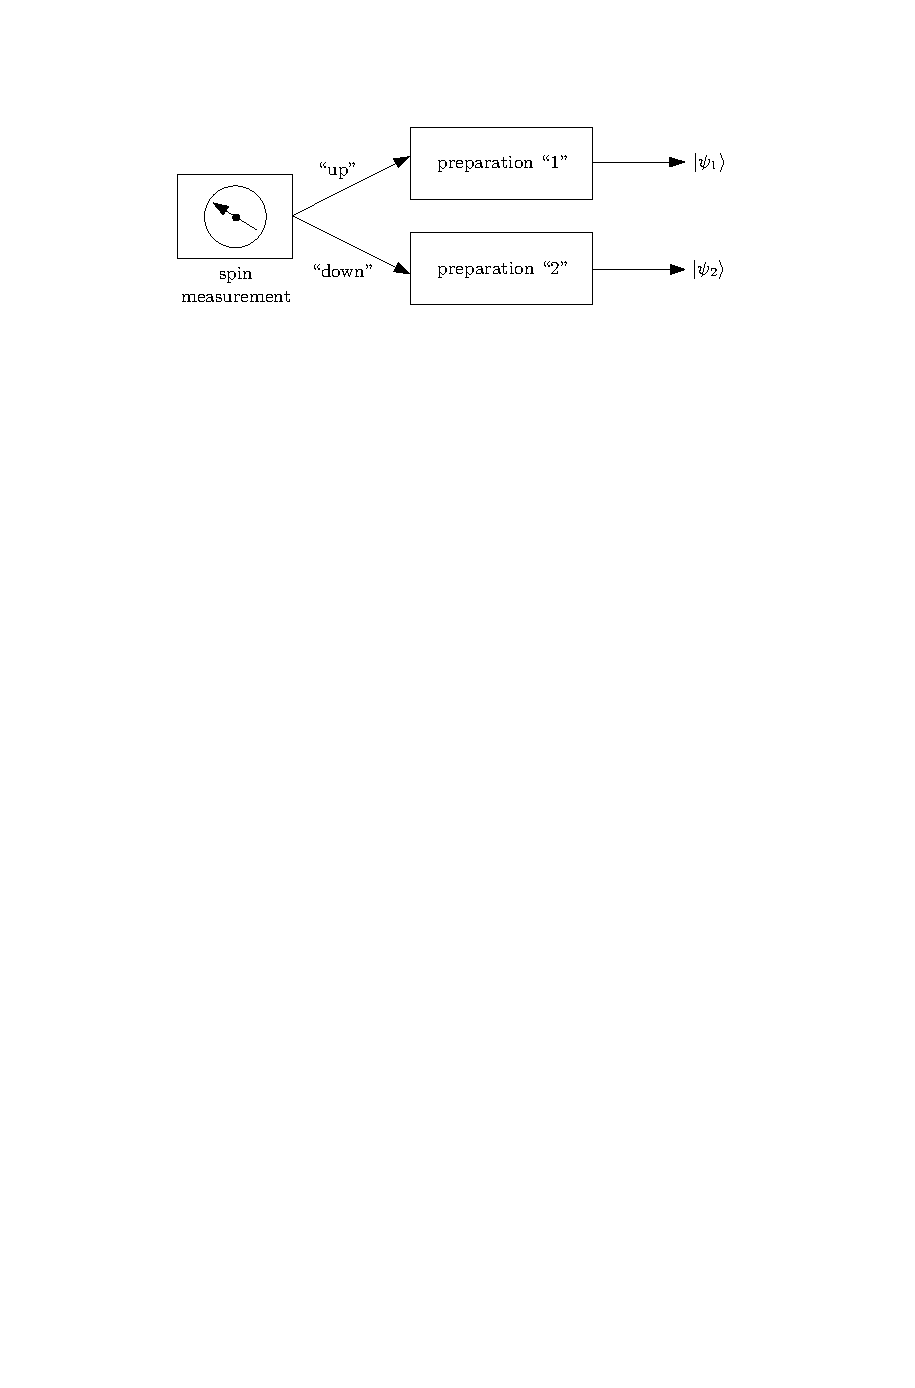
\includegraphics[width=.9\linewidth]{figures/ch02_fig03.pdf}\caption{確率的な状態準備手順の例。スピン$1/2$粒子のスピン測定の結果に応じて、装置は、ある系を量子状態$\lvert\psi_1\rangle$または$\lvert\psi_2\rangle$に準備する。具体的なスピン測定結果を知らない観測者は、状態$\lvert\psi_1\rangle$と$\lvert\psi_2\rangle$に、等しい古典的な確率を割り当てる。この主観的な無知を表すために、準備された系を、混合状態の密度行列$\hat\rho=\frac12\lvert\psi_1\rangle\langle\psi_1\rvert+\frac12\lvert\psi_2\rangle\langle\psi_2\rvert$で記述する。}\end{figure}

確率的要素の物理的な起源が何であれ、混合状態、すなわち確率$p_i$を伴う可能な純粋状態$\lvert\psi_i\rangle$の集合は、古典的な集団を表す。これは、確率の起源が純粋に古典的であることを意味する。これらの確率は、系の量子状態についての観測者の主観的無知を表すにすぎない。物理的には、系は実際に、純粋で、したがって完全に既知の状態に準備されている。ただし観測者には知られていない。原理上、状態準備の手順の各段階をすべて追跡、あるいは遡及すれば、各実行でどの純粋状態$\lvert\psi_i\rangle$が生成されたかを、必ず決められる。確率$p_i$は、準備手順の細かい詳細を調べないという私たちの実際的な選択を表すだけであり、これらの確率には根本的なものはない。したがって、たとえば気体中の個々の分子の決定論的経路を、原理上は追跡できても実際にはできない古典統計力学での「粗視化」と同じ方法に対応するだけである。

% 原文 p.38
\hypertarget{srcpage:38}{}\label{srcpage:38}
混合状態で記述される系について行った測定の統計を、観測者はどのように記述するだろうか。もはや系に純粋量子状態$\lvert\psi\rangle$を割り当てられないので、純粋状態の密度行列$\hat\rho=\lvert\psi\rangle\langle\psi\rvert$を用いた、通常の規則$\langle\hat O\rangle=\langle\psi\rvert\hat O\lvert\psi\rangle$、または$\langle\hat O\rangle=\operatorname{Tr}(\hat\rho\hat O)$［式(2.17)］により、観測可能量$\hat O$の期待値を計算できないことは明らかである。しかしこれらの規則は、準備された系の純粋状態を観測者が知らないことから生じる古典的な確率概念と、量子状態が測定される観測可能量の固有状態へ確率的に「収縮」することから生じる、量子力学固有の確率を組み合わせることで、容易に一般化できる。直観的な考えは、混合状態に含まれる可能な各純粋状態$\lvert\psi_i\rangle$での期待値$\langle\psi_i\rvert\hat O\lvert\psi_i\rangle$を、その状態の古典的確率$p_i$で重み付けし、集団全体について結果を足し合わせるだけである。すなわち、
\begin{equation}\langle\hat O\rangle=\sum_i p_i\langle\psi_i\rvert\hat O\lvert\psi_i\rangle.\tag{2.19}\end{equation}
この式には、まだ別々の二つの統計的要素、すなわち古典的確率$p_i$と、各純粋状態$\lvert\psi_i\rangle$での量子期待値$\langle\psi_i\rvert\hat O\lvert\psi_i\rangle$が含まれる。この両方を包含し、系のすべての統計的性質を完全に符号化する、混合状態の密度行列を導入できる。それは
\begin{equation}\hat\rho=\sum_i p_i\lvert\psi_i\rangle\langle\psi_i\rvert,\qquad p_i\ge0,\quad\sum_i p_i=1\tag{2.20}\end{equation}
で与えられる。これを、純粋状態の密度行列$\hat\rho_i=\lvert\psi_i\rangle\langle\psi_i\rvert$の古典的確率分布と見ることができる。

古典的確率の概念は、すでに混合状態の密度行列(2.20)に組み込まれているため、観測可能量$\hat O$の期待値は、純粋状態とまったく同じく、トレース則(2.17)で計算できる。すなわち、
\begin{equation}\langle\hat O\rangle=\operatorname{Tr}(\hat\rho\hat O).\tag{2.21}\end{equation}
当然ながら、これは、純粋な成分状態$\lvert\psi_i\rangle$で期待値を計算し、混合状態の確率$p_i$で重み付けする方法(2.19)と同値である。

純粋状態の密度行列と同じく、混合状態の密度行列も規格化条件(2.18)、
\begin{equation}\operatorname{Tr}\hat\rho=1\tag{2.22}\end{equation}
を満たす。これは、構成する各純粋状態の密度行列$\hat\rho_i=\lvert\psi_i\rangle\langle\psi_i\rvert$の規格化(2.18)と、$\sum_i p_i=1$から直ちに従う。
% 原文 p.39
\hypertarget{srcpage:39}{}\label{srcpage:39}
\begin{equation}\operatorname{Tr}\hat\rho=\sum_i p_i\operatorname{Tr}(\lvert\psi_i\rangle\langle\psi_i\rvert)\overset{(2.18)}=\sum_i p_i=1.\tag{2.23}\end{equation}
2.3節で論じたように、二つの部分系の量子もつれは、複合純粋状態$\lvert\Psi\rangle$を、純粋な部分系状態$\lvert\psi\rangle_1$、$\lvert\phi\rangle_2$のテンソル積$\lvert\Psi\rangle=\lvert\psi\rangle_1\lvert\phi\rangle_2$と書けないことに対応する。いま、この状況を密度行列の言葉で、同値に述べ直せる。複合系が、二つの部分系に属する密度行列$\hat\rho_1$、$\hat\rho_2$を用いて、テンソル積$\hat\rho=\hat\rho_1\otimes\hat\rho_2$と書けない、純粋状態または混合状態の密度行列$\hat\rho$で記述される場合、二つの部分系は互いにもつれている。この基準は、状態ベクトルによる上の量子もつれの定義から直接に従う。したがって、全密度行列が部分系の密度行列へ因数分解されるとき、$\hat\rho=\hat\rho_1\otimes\hat\rho_2\otimes\cdots$、これらの部分系間に量子的相関は存在しない。

最後に、重要な点を強調しすぎる恐れはあるが、混合状態は、次の形の純粋状態の重ね合わせと明確に区別しなければならない。
\begin{equation}\lvert\psi\rangle=\sum_i\sqrt{p_i}\lvert\psi_i\rangle.\tag{2.24}\end{equation}
2.2.1節で論じたように、ここではすべての成分状態$\lvert\psi_i\rangle$が同時に存在しており、これは少なくとも原理上、常に実験で検証できる。この重ね合わせには、先験的な確率的要素は含まれない。$\lvert\psi\rangle$は純粋状態であり、したがって系についての最大の知識を包含する。重ね合わせ(2.24)に対応する密度行列は、
\begin{equation}\begin{split}\hat\rho=\lvert\psi\rangle\langle\psi\rvert&=\sum_{ij}\sqrt{p_ip_j}\lvert\psi_i\rangle\langle\psi_j\rvert\\&=\sum_i p_i\lvert\psi_i\rangle\langle\psi_i\rvert+\sum_{i\ne j}\sqrt{p_ip_j}\lvert\psi_i\rangle\langle\psi_j\rvert.\end{split}\tag{2.25}\end{equation}
異なる状態$\lvert\psi_i\rangle$間の干渉を表す、非対角項$i\ne j$の存在が、この純粋状態の密度行列を、混合状態の密度行列(2.20)から明確に区別する。

% 原文 pp.39--44、2.4.3--2.4.5。
\subsubsectionlink{「混合の程度」の定量化}
純粋状態の密度行列$\hat\rho=\lvert\psi\rangle\langle\psi\rvert$は、純粋状態$\lvert\psi\rangle$への射影演算子にすぎないので、直ちに
\begin{equation}\hat\rho^2=\hat\rho\tag{2.26}\end{equation}
が従う。この射影演算子の性質$\hat\rho^2=\hat\rho$は、実際、系が純粋状態にあるための必要十分条件をなす。次の議論でそれが分かる。系が純粋状態になく、代わりに、少なくとも二つの非零の確率$p_i$を持つ混合状態の密度行列(2.20)で記述されているとする。この密度行列については、
% 原文 p.40
\hypertarget{srcpage:40}{}\label{srcpage:40}
\begin{equation}\hat\rho^2=\sum_{ij}p_ip_j\lvert\psi_i\rangle\langle\psi_j\rvert\langle\psi_i\vert\psi_j\rangle\tag{2.27}\end{equation}
を得る。まず、一般に$i\ne j$に対して$\langle\psi_i\vert\psi_j\rangle\ne0$であるが、仮に$i\ne j$で$\langle\psi_i\vert\psi_j\rangle=0$でも、結局
\begin{equation}\hat\rho^2=\sum_i p_i^2\lvert\psi_i\rangle\langle\psi_i\rvert\tag{2.28}\end{equation}
を得る。各$p_i$の値は1未満なので、この式は$\hat\rho$［式(2.20)］と異なる。したがって、任意の密度行列$\hat\rho$が与えられたら、式(2.26)、すなわち$\hat\rho^2=\hat\rho$が成り立つかを調べるだけで、系が純粋状態にあるかどうかを容易に判定できる。

さらに一歩進み、与えられた密度行列が純粋かどうかを示すだけでなく、次の意味でその「混合の程度」を定量化する尺度を定義できる。再び式(2.20)の混合状態の密度行列、
\begin{equation}\hat\rho=\sum_i p_i\lvert\psi_i\rangle\langle\psi_i\rvert\tag{2.29}\end{equation}
を考えよう。すでに分かっているように、純粋状態の密度行列の場合は、一つ、たとえば$p_1=1$を除くすべての$p_i$が零であることに対応する。すなわち、この状況では系の状態について「無知」はない。いま$p_1$の大きさを減らすとしよう。確率の規格化条件$\sum_i p_i=1$によれば、そのとき少なくとも一つの、$p_1$とは別の$p_i$が非零の値、たとえば$p_2>0$を取らなければならない。いまや、系が純粋状態$\lvert\psi_1\rangle$、$\lvert\psi_2\rangle$のどちらに準備されたかを確実には知らないので、ある程度の「無知」が存在する。それでも、たとえば$p_1=90\%$、$p_2=10\%$なら、状態$\lvert\psi_1\rangle$が準備されたと、かなりの自信を持てる。したがって「混合の程度」は低い。純粋状態の反対の極限は、密度行列が単位演算子に比例するときに達する。これは、系のHilbert空間の基底をなす、互いに直交する純粋状態の、等しい重みの集団に対応する。この場合、密度行列は、どの純粋状態が準備されたかについて、いかなる情報も含まず、したがって最大の無知、すなわち「混合の程度」を表す。

次に、混合の程度をより一般的に定量化する二つの尺度を導入しよう。単純で広く用いられる尺度は、密度行列の純度であり、
\begin{equation}\varsigma\equiv\operatorname{Tr}(\hat\rho^2)\tag{2.30}\end{equation}
と定義される。なぜこれが適切な尺度なのだろうか。$\hat\rho$が純粋状態の密度行列を表すなら、式(2.18)、(2.26)から$\varsigma=1$が従う。他方、状態$\{\lvert\psi_i\rangle\}$が、系の$N$次元Hilbert空間の正規直交基底をなすと仮定すると、混合状態の密度行列(2.20)の純度は、式(2.28)より
% 原文 p.41
\hypertarget{srcpage:41}{}\label{srcpage:41}
\begin{equation}\varsigma=\sum_{i=1}^N p_i^2\tag{2.31}\end{equation}
である。この和の下限は$1/N$であり、密度行列が最大混合であるとき、すなわち、すべての$i=1,\ldots,N$について$p_i=1/N$であるときに、ちょうどこの値を取る。

密度行列の純粋さ、または不純さを定量化する、もう一つの広く用いられる尺度は、von Neumannエントロピーである。この尺度は、1927年に数学者John von Neumannが初めて導入し\cite{ref059}、その後、彼の記念碑的な量子力学の著書\cite{ref060}でさらに発展させた（興味深い歴史的考察は文献\cite{ref061}も参照）。von Neumannエントロピーは、古典統計力学のエントロピーの概念を、量子力学の密度演算子へ一般化したものと見なせる。それは
\begin{equation}S(\hat\rho)\equiv-\operatorname{Tr}(\hat\rho\log_2\hat\rho)\equiv-\sum_i\lambda_i\log_2\lambda_i\tag{2.32}\end{equation}
で与えられる。ここで$\lambda_i$は密度行列$\hat\rho$の固有値である。慣例により、$\lambda_i=0$の場合は$0\log_2(0)\equiv0$と定義して扱う。これにより、混合に含まれない状態は、当然ながらエントロピーの値に寄与しない。

再び、この尺度の具体的な値を求めよう。$\hat\rho$が純粋なら、一つを除くすべての$\lambda_i$が零で、残りの一つは1を取らなければならないため、$S(\hat\rho)=0$である。したがって純粋状態は、von Neumannエントロピーが零であることによって特徴付けられる。他方、互いに排他的で、したがって直交する純粋状態$\lvert\psi_i\rangle$（$i=1,\ldots,N$）のどれを準備したかについての完全な無知に対応する、最大混合状態では、$\lambda_i=p_i=1/N$だから、
\begin{equation}S(\hat\rho)=\log_2(N)\tag{2.33}\end{equation}
を得る。これは$S(\hat\rho)$が取りうる最大値である。中間の、最大混合でない状態では、それに応じて値は小さくなる。たとえば準備装置が、直交する状態の部分集合$\lvert\psi_i\rangle$（$i=1,\ldots,M<N$）だけを等しい確率で準備するなら、$S(\hat\rho)=\log_2(M)$を得る。これらの値は、von Neumannエントロピーの定義が、古典的、すなわち熱力学的な状況でのエントロピーの直観と一致することを示す。そこではエントロピーは、系の状態についての情報量、または逆に無知の量の尺度であり、典型的には、系が利用できる異なる可能な状態の数によって定量化される。

\subsubsectionlink{混合状態の密度行列の基底の曖昧さ}
上の2.4.2節では、混合状態の概念が古典的確率概念に基づくことを論じた。したがって、混合状態の密度行列(2.20)は、純粋状態の、無知として解釈可能な真正混合を表すとも言う\cite{ref047,ref048,ref049}\footnote{この分類は、縮約密度行列を導入するとき（2.4.6節）に重要となる。縮約密度行列は、無知として解釈できないことが分かる。}。これは式(2.20)の形の混合状態の密度行列を、ある程度まで、純粋量子状態$\lvert\psi_i\rangle$の古典的確率分布と解釈できることを表現している。しかし、それが正しいのは、系が実際に状態$\lvert\psi_i\rangle$の一つに準備されたことを知っていて、単にどの状態かについての、より具体的な情報を持たない場合だけである。他方、密度行列(2.20)だけを与えられ、たとえば準備手順などの追加情報がなければ、系が実際に状態$\lvert\psi_i\rangle$の一つにあるとは推論できない。なぜなら、非純粋な密度行列はどれも、多くの異なる方法で書くことができ、特定の量子状態の集団への分割はいずれも任意であることを示しているからである。言い換えれば、混合状態の密度行列だけでは、純粋状態の古典的確率分布を一意に再構成できない。

% 原文 p.42
\hypertarget{srcpage:42}{}\label{srcpage:42}
これを説明するため、混合状態の密度行列
\begin{equation}\hat\rho=\frac12\lvert0_z\rangle\langle0_z\rvert+\frac12\lvert1_z\rangle\langle1_z\rvert\tag{2.34}\end{equation}
を考えよう。このような密度行列は、Pauliスピン演算子$\hat\sigma_z$の固有状態$\lvert0_z\rangle$、$\lvert1_z\rangle$のどちらか一方に、等しい確率で準備された系を記述する際に用いる。ただし、どちらかは知らないので、これらの状態の古典的確率分布による記述に頼らざるをえない。

他方、状態$\lvert0_z\rangle$、$\lvert1_z\rangle$は、$x$軸方向のスピンに対するPauli演算子$\hat\sigma_x$の固有状態$\lvert0_x\rangle$、$\lvert1_x\rangle$によっても書き直せる。
\begin{equation}\begin{split}\lvert0_z\rangle&=\frac1{\sqrt2}(\lvert0_x\rangle+\lvert1_x\rangle),\\\lvert1_z\rangle&=\frac1{\sqrt2}(\lvert0_x\rangle-\lvert1_x\rangle).\end{split}\tag{2.35}\end{equation}
これらを用いれば、密度行列(2.34)は同値に
\begin{equation}\hat\rho=\frac12\lvert0_x\rangle\langle0_x\rvert+\frac12\lvert1_x\rangle\langle1_x\rvert\tag{2.36}\end{equation}
と書ける。実際、$\hat\rho$は、任意の軸に沿ったスピン固有状態を用いて、この形に無限通りに書き直せる。したがって、系のスピン状態をどの物理的な軸に沿って準備したかを知らない限り、密度行列だけが与えるのは、異なる純粋状態の集合の確率についての情報だけであり、具体的にどの集合の状態を準備したかという情報ではない。ここで、その集合は$\{\lvert0_z\rangle,\lvert1_z\rangle\}$、$\{\lvert0_x\rangle,\lvert1_x\rangle\}$などで表される。

% 原文 p.43
\hypertarget{srcpage:43}{}\label{srcpage:43}
\subsubsectionlink{混合状態の密度行列と物理的集団}
ここで重要な注意を述べておく。式(2.20)の形の混合状態の密度行列$\hat\rho=\sum_i p_i\lvert\psi_i\rangle\langle\psi_i\rvert$は、同一の系$\mathcal S_k$（$k=1,\ldots,N$）の物理的集団、すなわち、特定の関心のある系の「コピー」の集まりを記述するためにも、しばしば用いられる。各系は、純粋状態$\lvert\psi_i\rangle$（$i=1,\ldots,M\le N$）の一つに決定論的に準備されている。量$p_i$は、今度は状態$\lvert\psi_i\rangle$に準備された系の割合を表す。この「集団」による方法は、密度行列の概念を導入する動機付けとして、教科書に頻繁に見られる（たとえば文献\cite{ref058}）。

しかし、物理的な集団と統計的な混合の間には、重要な区別が必要である。集団の場合、混合状態の密度行列による記述を正当化する情報の不足は、何もない（もちろん、個々の系自体が純粋状態に準備されていない場合は別である）。むしろ、すべての個々の系$\mathcal S_k$の集団は、各系$\mathcal S_k$の$N$個の状態空間$\mathcal H_k$のテンソル積であるHilbert空間$\mathcal H$によって記述しなければならない。
\begin{equation}\mathcal H=\bigotimes_{k=1}^N\mathcal H_k.\tag{2.37}\end{equation}
同様に、全系$\mathcal S$は、個々の状態$\lvert\psi_k\rangle\in\{\lvert\psi_i\rangle\}$の、純粋なテンソル積状態$\lvert\Psi\rangle$で記述される。
\begin{equation}\lvert\Psi\rangle=\left(\prod_{j=1}^{Np_1}\lvert\psi_1\rangle\right)\left(\prod_{j=1}^{Np_2}\lvert\psi_2\rangle\right)\cdots\left(\prod_{j=1}^{Np_M}\lvert\psi_M\rangle\right).\tag{2.38}\end{equation}
したがって、対応する$N$系の純粋密度行列$\hat\rho=\lvert\Psi\rangle\langle\Psi\rvert$は、一系の純粋状態$\lvert\psi_i\rangle$の確率分布を記述する混合状態の密度行列の式(2.20)とは、明らかに異なる。

物理系の集団を一系の混合状態の密度行列で記述することが正当化されるのは、集団平均という、限定された純粋に統計的な意味においてだけである。これは、集団内の一系の測定に話を限り、集団全体の平均的統計を考える場合である。具体的には、$N$系の純粋状態(2.38)で記述される集団の各要素について、一系の観測可能量$\hat O$を測定し、結果を集団全体で平均すれば、
\begin{equation}\langle\hat O\rangle=\frac1N\sum_{i=1}^M Np_i\langle\psi_i\rvert\hat O\lvert\psi_i\rangle\tag{2.39}\end{equation}
を得る。簡単のため、$\lvert\psi_i\rangle$は個々の系ごとに、正規直交基底状態の組をなすと仮定した。代わりに、混合状態$\hat\rho$［式(2.20)］における$\hat O$の期待値を、トレース則を使って計算すると、同じ結果
% 原文 p.44
\hypertarget{srcpage:44}{}\label{srcpage:44}
\begin{equation}\langle\hat O\rangle=\sum_{i=1}^M p_i\operatorname{Tr}(\hat\rho\hat O)=\sum_{i=1}^M p_i\langle\psi_i\rvert\hat O\lvert\psi_i\rangle\tag{2.40}\end{equation}
を得る。したがって一系の観測可能量については、集団平均において、しかもこの平均においてのみ、$N$系の純粋状態$\lvert\Psi\rangle$に対応する純粋状態密度行列が生む統計は、一系の混合状態の密度行列(2.20)から得られる統計と一致する。これに対し、集団を$N$系の純粋状態として正しく記述する式(2.38)によれば、系の集団の任意の観測可能量についても、各個別の系についても、統計を計算できる。

% 原文 pp.44--49、2.4.6全体。
\subsubsectionlink{縮約密度行列}
縮約密度行列は、デコヒーレンスの形式的記述において重要な役割を果たし、その起源は量子力学の初期に遡る\cite{ref060,ref062,ref063}（興味深い考察は文献\cite{ref064}も参照）。縮約密度行列の概念の基本的な動機は、他の系$\mathcal B$と量子的に相関している、すなわちもつれている量子系$\mathcal A$を記述することである。この場合、全複合系$\mathcal{AB}$の量子状態は純粋であってよく、したがって原理上は完全に既知でありうる。しかし、観測者が最初の系$\mathcal A$にしかアクセスできず、$\mathcal A$についてだけ測定を行え、$\mathcal B$については行えないとしよう。その場合、複合系の状態について知りうることはすべて、$\mathcal A$だけに対する局所的な測定から導かなければならず、その測定は、この系で可能な測定結果と、その確率分布を与える。そこで中心的な問いは、次のようになる。系$\mathcal A$の観測者が引き出せるすべての情報、すなわち、すべての測定統計を、過不足なく正しく含む、量子力学の形式内で適切な数学的対象は何か。

その対象は、次式で与えられる縮約密度行列であることが分かる。
\begin{equation}\hat\rho_{\mathcal A}\equiv\operatorname{Tr}_{\mathcal B}\hat\rho.\tag{2.41}\end{equation}
添字「$\mathcal B$」は、$\mathcal B$のHilbert空間$\mathcal H_{\mathcal B}$の正規直交基底だけを用いて、トレースを取ることを意味する。そのため演算「$\operatorname{Tr}_{\mathcal B}$」は、$\mathcal B$にわたる部分トレースとも呼ばれ、観測されない系$\mathcal B$の自由度についての「平均」と解釈できる。この解釈は後にさらに明らかになる。したがって式(2.41)は、系$\mathcal A$だけに属するすべての観測可能量の測定統計が、$\mathcal A$と量子的に相関している$\mathcal B$の自由度の「トレースを取って消去」して得た縮約密度行列$\hat\rho_{\mathcal A}$に、完全に含まれることを意味する。

% 原文 p.45
\hypertarget{srcpage:45}{}\label{srcpage:45}
\paragraph{デコヒーレンスとの関係}
式(2.41)を導く前に、まずデコヒーレンスの記述における縮約密度行列の概念の重要性を論じよう。デコヒーレンスは、二つの系、すなわち「関心のある系」と、その環境との間の相互作用から生じることを思い出そう。通常、そのような相互作用は、系と環境を合わせたもののもつれ状態をもたらす。普通、観測者は関心のある系だけについて測定し、環境は通常、アクセス不能か、完全には測定できないか、あるいは単に関心の対象ではない。たとえば、物体に散乱される光子からなる環境を考えてよい。実際上、散乱された光子をすべて捕らえることは通常不可能なので、観測者が測定できるのは、系と環境光子の一部に属する観測可能量だけである。

ここで縮約密度行列が役に立つ。系と環境の密度行列について、環境の自由度の全部または一部にわたりトレースを取ると、系の縮約密度行列によって、関心のある系の測定統計の完全で網羅的な記述を得られる。系に対する局所測定への環境の影響は、すべて自動的に、この縮約密度行列に包含される。系は環境ともつれているので、系自体に個別の量子状態を帰属させることはできない。したがって、系の測定統計を記述するために利用できるのは、縮約密度行列だけであり\footnote{Zurekが最近発展させた、いわゆる「envariance」の研究計画\cite{ref016,ref065,ref066,ref067}は、8.2.2節で概説するように、もつれ状態の対称性を使う。この計画は、ある仮定の集合のもとで、縮約密度行列を用いず、したがってBorn則を前提とせずに、他の系ともつれた系の状態と測定を論じられる枠組みを与える。}、この縮約密度行列は、系と環境の量子もつれの存在により、必ず非純粋になる。

\paragraph{縮約密度行列の導出}
縮約密度行列の式(2.41)を導こう。そのため、二つの系$\mathcal A$、$\mathcal B$の、次の形のもつれ状態を考える。
\begin{equation}\lvert\Psi\rangle=\frac1{\sqrt2}(\lvert a_1\rangle\lvert b_1\rangle+\lvert a_2\rangle\lvert b_2\rangle).\tag{2.42}\end{equation}
ここで$\lvert a_i\rangle$と$\lvert b_i\rangle$（$i=1,2$）は、それぞれ$\mathcal A$、$\mathcal B$の任意の規格化された状態であり、必ずしも直交していない。式(2.11)から、対応する純粋状態の密度行列は、
\begin{equation}\hat\rho=\lvert\Psi\rangle\langle\Psi\rvert=\frac12\sum_{i,j=1}^2\lvert a_i\rangle\langle a_j\rvert\otimes\lvert b_i\rangle\langle b_j\rvert\tag{2.43}\end{equation}
である。また、$\{\lvert\psi_k\rangle\}$、$\{\lvert\phi_l\rangle\}$を、それぞれ$\mathcal A$、$\mathcal B$のHilbert空間$\mathcal H_{\mathcal A}$、$\mathcal H_{\mathcal B}$の正規直交基底とする。

% 原文 p.46
\hypertarget{srcpage:46}{}\label{srcpage:46}
系$\mathcal A$だけに作用する観測可能量を考えよう。それは$\hat O=\hat O_{\mathcal A}\otimes\hat I_{\mathcal B}$と書ける。ここで$\hat I_{\mathcal B}$は、$\mathcal B$のHilbert空間の単位演算子である。先ほど提起した問いに従い、二部分系の密度行列(2.43)より単純でありながら、このような$\mathcal A$の観測可能量すべての期待値を計算できる、数学的対象が存在するかを調べたい。

すでに知っているように、任意の観測可能量の期待値$\langle\hat O\rangle$は、標準的なトレース則(2.17)、$\langle\hat O\rangle=\operatorname{Tr}(\hat\rho\hat O)$で計算できる。いま$\hat O=\hat O_{\mathcal A}\otimes\hat I_{\mathcal B}$なので、系$\mathcal B$に属するトレース演算の部分を直ちに実行できる。具体的には、
\begin{equation}\begin{split}
\langle\hat O\rangle&=\operatorname{Tr}(\hat\rho\hat O)\\
&=\sum_{kl}\langle\phi_l\rvert\langle\psi_k\rvert\hat\rho(\hat O_{\mathcal A}\otimes\hat I_{\mathcal B})\lvert\psi_k\rangle\lvert\phi_l\rangle\\
&=\sum_k\langle\psi_k\rvert\left(\sum_l\langle\phi_l\rvert\hat\rho\lvert\phi_l\rangle\right)\hat O_{\mathcal A}\lvert\psi_k\rangle\\
&=\sum_k\langle\psi_k\rvert(\operatorname{Tr}_{\mathcal B}\hat\rho)\hat O_{\mathcal A}\lvert\psi_k\rangle\\
&\equiv\sum_k\langle\psi_k\rvert\hat\rho_{\mathcal A}\hat O_{\mathcal A}\lvert\psi_k\rangle\\
&=\operatorname{Tr}_{\mathcal A}(\hat\rho_{\mathcal A}\hat O_{\mathcal A}).
\end{split}\tag{2.44}\end{equation}
ここで$\hat\rho_{\mathcal A}$は、まさに式(2.41)で導入した縮約密度行列である。

縮約密度行列の概念は、二部分系のもつれ状態から、$N$個の部分系間の量子もつれを記述する任意の純粋状態$\lvert\psi\rangle$へ一般化できる。系$i$だけに属する観測可能量$\hat O$、
\begin{equation}\hat O=\hat I_1\otimes\hat I_2\otimes\cdots\otimes\hat I_{i-1}\otimes\hat O_i\otimes\hat I_{i+1}\otimes\cdots\otimes\hat I_N\tag{2.45}\end{equation}
を考える。トレース則を適用して得る$\hat O$の測定統計は、$N$個すべての部分系を含む複合系の純粋状態の密度行列$\hat\rho=\lvert\Psi\rangle\langle\Psi\rvert$を使っても、第$i$部分系の縮約密度行列
\begin{equation}\hat\rho_i=\operatorname{Tr}_{1,\ldots,i-1,i+1,\ldots,N}(\hat\rho)\tag{2.46}\end{equation}
を使っても同じになる。後者は、第$i$部分系を除くすべての部分系についてトレースを取って得られる。これは、
\begin{equation}\langle\hat O\rangle=\operatorname{Tr}(\hat\rho\hat O)=\operatorname{Tr}_i(\hat\rho_i\hat O_i)\tag{2.47}\end{equation}
が容易に示されるからである。

% 原文 p.47
\hypertarget{srcpage:47}{}\label{srcpage:47}
\paragraph{干渉の局所的測定可能性と識別可能性}
二部分系の状態(2.42)については、全密度行列$\hat\rho$の式(2.43)から、$\hat\rho_{\mathcal A}$［式(2.44)］を容易に計算できる。$\mathcal B$の状態$\lvert b_i\rangle$（$i=1,2$）を、$\mathcal H_{\mathcal B}$の正規直交基底ベクトルの組$\{\lvert\phi_l\rangle\}$で
\begin{equation}\lvert b_i\rangle=\sum_l c_l^{(i)}\lvert\phi_l\rangle\tag{2.48}\end{equation}
と展開すれば、
\begin{equation}\begin{split}
\hat\rho_{\mathcal A}&=\operatorname{Tr}_{\mathcal A}\left(\frac12\sum_{i,j=1}^2\lvert a_i\rangle\langle a_j\rvert\otimes\lvert b_i\rangle\langle b_j\rvert\right)\\
&=\frac12\sum_{i,j=1}^2\lvert a_i\rangle\langle a_j\rvert\sum_k\langle\phi_k\rvert\left(\sum_{ll'}c_l^{(i)}(c_{l'}^{(j)})^*\lvert\phi_l\rangle\langle\phi_{l'}\rvert\right)\lvert\phi_k\rangle\\
&=\frac12\sum_{i,j=1}^2\lvert a_i\rangle\langle a_j\rvert\sum_k c_k^{(i)}(c_k^{(j)})^*\\
&=\frac12\sum_{i,j=1}^2\lvert a_i\rangle\langle a_j\rvert\langle b_j\vert b_i\rangle\\
&=\frac12\bigl(\lvert a_1\rangle\langle a_1\rvert+\lvert a_2\rangle\langle a_2\rvert\\
&\hspace{17mm}+\lvert a_1\rangle\langle a_2\rvert\langle b_2\vert b_1\rangle+\lvert a_2\rangle\langle a_1\rvert\langle b_1\vert b_2\rangle\bigr)
\end{split}\tag{2.49}\end{equation}
を得る。この結果は、複合系$\mathcal{AB}$が二成分状態(2.42)ではなく、$N>2$の、より一般的な$N$成分状態$\lvert\Psi\rangle=N^{-1/2}\sum_{n=1}^N\lvert a_n\rangle\lvert b_n\rangle$で記述される場合にも、容易に一般化できる。その場合、縮約密度行列は
\begin{equation}\hat\rho_{\mathcal A}=\frac1N\sum_{i,j=1}^N\lvert a_i\rangle\langle a_j\rvert\langle b_j\vert b_i\rangle\tag{2.50}\end{equation}
となる。式(2.49)から、測定統計への系$\mathcal B$の影響は、縮約密度行列の非対角項$\lvert a_1\rangle\langle a_2\rvert$、$\lvert a_2\rangle\langle a_1\rvert$に掛かる、$\mathcal B$の状態$\lvert b_1\rangle$と$\lvert b_2\rangle$の重なり$\langle b_2\vert b_1\rangle=\langle b_1\vert b_2\rangle^*$へ、実効的にまとめられることが分かる。2.4.2節で述べたように、これらの非対角項は、状態$\lvert a_1\rangle$、$\lvert a_2\rangle$間の干渉に対応する。

したがって、非常に重要な結果を得る。$\mathcal A$の状態$\lvert a_1\rangle$、$\lvert a_2\rangle$と一対一に相関した、$\mathcal B$の相対状態$\lvert b_1\rangle$、$\lvert b_2\rangle$の重なりの大きさ［式(2.42)］は、$\mathcal A$で測定できる$\{\lvert a_1\rangle,\lvert a_2\rangle\}$基底の干渉の程度を定量化する。これは2.3.2節の先の考察に直結する。そこでは、二部分系の純粋状態に存在するもつれの程度を、一方の部分系に符号化された、他方の対応する相対状態に関する情報量によって、直観的に導入した。この尺度を、一方の部分系の関連する状態の識別可能性に結び付け、それらの相互の重なりによって定量化した。こうして、もつれの程度、識別可能性の大きさ、そして一方の部分系だけを測定して干渉を観測できる程度の間の、密接なつながりが見える。

% 原文 p.48
\hypertarget{srcpage:48}{}\label{srcpage:48}
たとえば、状態$\lvert b_1\rangle$、$\lvert b_2\rangle$の重なりが消失し、したがって完全に識別可能になる極限では、縮約密度行列(2.49)は$\{\lvert a_1\rangle,\lvert a_2\rangle\}$基底で対角となる。
\begin{equation}\hat\rho_{\mathcal A}=\frac12(\lvert a_1\rangle\langle a_1\rvert+\lvert a_2\rangle\langle a_2\rvert).\tag{2.51}\end{equation}
非対角の干渉項$\lvert a_1\rangle\langle a_2\rvert$、$\lvert a_2\rangle\langle a_1\rvert$がなくなるため、状態$\lvert a_1\rangle$、$\lvert a_2\rangle$間の干渉を測定できる局所的な観測可能量$\hat O=\hat O_{\mathcal A}\otimes\hat I_{\mathcal B}$は存在しない。

\paragraph{縮約密度行列と集団}
ここで重要な注意を述べる。明らかに、縮約密度行列(2.51)は、系$\mathcal A$が真正混合で記述される場合に得る密度行列と、形式上同一である。そのような真正混合は、二つの純粋状態$\lvert a_1\rangle$、$\lvert a_2\rangle$の一方に、系が等しい確率である状況に対応することを思い出そう。これは、両成分$\lvert a_1\rangle$、$\lvert a_2\rangle$が存在する、大域的にもつれた重ね合わせ(2.42)と対照的である。後者は、少なくとも原理上、適切な干渉実験によって常に確かめられる（2.2.1節）。

系$\mathcal A$ともつれた系$\mathcal B$の自由度についてトレースを取って得る縮約密度行列(2.51)と、混合状態の密度行列が形式上同一であることは、$\mathcal A$だけに属する観測可能量の測定では、純粋状態と混合状態という二つの場合を区別できないことを意味する\footnote{混合状態と純粋状態を操作的に区別できないことは、実際には、局所測定への制限の帰結にとどまらず、$\hat O=\hat O_{\mathcal A}\otimes\hat O_{\mathcal B}$の形に因数分解される複合系の任意の観測可能量についても成り立つことを示せる（たとえば文献\cite[pp.~208--210]{ref068}）。ここで$\hat O_{\mathcal A}$、$\hat O_{\mathcal B}$は、それぞれ$\mathcal A$、$\mathcal B$のHilbert空間における射影演算子$\lvert a_i\rangle\langle a_i\rvert$、$\lvert b_i\rangle\langle b_i\rvert$（$i=1,2$）と可換ではない。}。しかし、この形式上の同一性を、系の状態も混合と見なせることを意味すると解釈してはならないと理解することが、決定的に重要である（d'Espagnatの議論\cite{ref047,ref048,ref049}も参照）。一般に、密度行列は、可能な測定結果の集合の確率分布を計算する道具にすぎず、系の状態を指定しない。二つの系$\mathcal A$と$\mathcal B$はもつれており、全複合系は依然として重ね合わせ(2.42)で記述されているので、量子力学の標準的規則から、どちらの部分系にも、個別の確定した状態を帰属させられないことが従う。したがって、もつれた部分系の縮約密度行列は、非真正混合を表す\cite{ref047,ref048,ref049}。

% 原文 p.49
\hypertarget{srcpage:49}{}\label{srcpage:49}
そのため、縮約密度行列が混合状態の密度行列に形式上似ていることをもって、系$\mathcal B$との物理的相互作用と、形式的なトレース演算によって、大域的にもつれた重ね合わせ状態(2.42)から、どういうわけか魔法のように確定した部分系状態、すなわち、縮約密度行列(2.51)が示すような、等しい確率の$\lvert a_1\rangle$または$\lvert a_2\rangle$が得られた、と論じることはできない。この考察は、量子測定問題に対するデコヒーレンスの含意を論じるときに重要になる（次の2.5節）。第8章、特に8.1節でも、この問題に戻る。

% 原文 pp.49--55、2.5節導入、2.5.1--2.5.2。
\subsectionlink{測定問題と量子から古典への移行}
この節では、本文ですでに何度か触れた、よくも悪くも有名な量子力学の測定問題を述べる。「測定問題」という用語が選ばれた理由は、純粋に歴史的なものである。測定問題に関連する、ある種の基礎的問題が、系と相互作用する測定装置の量子力学的記述という文脈で、初めて示されたのである。

しかし「測定問題」という用語は、主として次の二つの理由から、範囲が狭すぎるとも考えられる。第一に、以下で見るように、測定問題は異なる三つの問題からなるので、むしろ複数の「測定問題」と言うのが適切だろう。第二に、量子測定と、そこで生じる基礎的問題は、量子から古典への移行という、より一般的な問題の特殊な場合にすぎない。後者は、基礎にある量子的領域から、私たちの周囲の実効的に古典的な系と性質が、どう現れるかという問いである。

したがって一方で、量子から古典への移行の問題は、文字どおりの量子測定の問題より、はるかに広い範囲を持つ。しかし他方で、物理系間の多くの相互作用は、測定に似た相互作用と見なせる。たとえば物体で散乱された光は、物体の位置に関する情報を持ち去るので、この意味で、入射光子を「測定装置」と見なせる。このように遍在する、測定に似た相互作用こそが、デコヒーレンスによる量子から古典への移行の説明の核心にある。より一般的な意味での測定は、量子から古典への移行という広い文脈でも、引き続き最重要の位置を占める。このことが、「測定問題」を完全に捨てて、より一般的な「量子から古典への移行の問題」に置き換えない理由となる。

% 原文 p.50
\hypertarget{srcpage:50}{}\label{srcpage:50}
上に示したように、測定問題、そして量子から古典への移行の問題は、三つの部分からなり、そのすべてを以下でより詳しく述べる。
\begin{enumerate}
\item 優先基底の問題（2.5.2節）。自然界で優先される物理量を、何が選び出すのか。たとえば、なぜ物理系は通常、位置の重ね合わせではなく、確定した位置に観測されるのか。
\item 干渉が観測されない問題（2.5.3節）。特に巨視的尺度で、なぜ量子干渉効果を観測するのは、それほど難しいのか。
\item 結果の問題（2.5.4節）。そもそも、なぜ測定には結果があり、量子確率分布が記述する異なる可能性のうち、何が特定の結果を選ぶのか。
\end{enumerate}
デコヒーレンスの適用範囲、成果、および含意を正しく理解するには、これらの問題に精通することが重要になる。先取りすれば、デコヒーレンスは最初の二つの問題を本質的に解決したと結論するのが、公平である。これらの問題とその解決は、量子力学の標準的形式の内部で、純粋に操作的な言葉で定式化できるので、これら二つに対処する際にデコヒーレンスが果たす役割は、ほとんど争われていない。

これに対し、第三の問題、すなわち結果の問題に取り組むうえでのデコヒーレンスの成功は、なお議論の対象である。特にこの問題は、量子力学の特定の解釈の選択と、ほとんど不可分に結び付いているからである（それは大部分、個人的な好みの問題に帰着する）。実際、デコヒーレンスが「その」測定問題を解けるかについての、過度に楽観的または悲観的な主張の大半は、より解釈的な結果の問題を解決するうえで、デコヒーレンスという標準的な量子効果が持ちうる適用範囲についての、誤解に遡れる。

\subsubsectionlink{理想的量子測定に対するvon Neumannの方式}
二つの別々の、もつれていない系から出発して、もつれた複合状態はどう生じるのだろうか。二つの部分系が個別性を失って、量子力学的な全体となるのは、どうして可能なのか。量子もつれは、重ね合わせ原理という運動学的概念と、Schrödinger時間発展の線形性という力学的性質の組合せから生じると見なせる。その結果としての過程は、しばしばvon Neumann測定として表される。これはvon Neumannが量子力学の初期に考案し、1932年の画期的な著書\cite{ref060}で論じた方式である。

von Neumannの目標は、系だけでなく装置、そして最終的には観測者（9.2節）をも量子力学的対象として扱い、量子測定という行為を、測定される系と測定装置の物理的相互作用として、完全に量子力学の言葉で記述することだった。この方法は、量子力学の法則に従わない、本質的に古典的な測定装置の存在を仮定していたCopenhagen解釈からの、根本的な離脱であったことに注意したい（8.1節）。

% 原文 p.51
\hypertarget{srcpage:51}{}\label{srcpage:51}
その名前にもかかわらず、von Neumann測定方式の適用範囲は、実際の意味での量子測定の文脈を、はるかに超える。実際、von Neumann方式は、量子もつれがどう生じるかを理解する最も容易な方法である。また、上に述べた測定問題の三つの成分、すなわち優先基底の問題、干渉効果が観測されない問題、および結果の問題を、うまく示す。最後に、系と環境の間のvon Neumann型の測定相互作用の帰結としてデコヒーレンスを見なすことにより、その基本的な形式を導入できる。

これらの導入的な注意を踏まえ、von Neumann測定方式を定式化しよう。その典型的な構成要素は、基底ベクトル$\{\lvert s_i\rangle\}$を持つHilbert空間$\mathcal H_{\mathcal S}$で記述される、通常は微視的な系$\mathcal S$と、Hilbert空間$\mathcal H_{\mathcal A}$の基底ベクトル$\{\lvert a_i\rangle\}$で形式的に表される、通常は巨視的な測定装置$\mathcal A$である。厳密に言えば、系と装置が微視的か巨視的かは、以下の一般的議論に影響しない。ただし、系を重ね合わせ状態へ容易に準備できることを確保したいので、物理的には通常、系を微視的なものと結び付けるのが妥当である。他方、測定装置の物理的実現は、通常、多数の自由度を持つ巨視的な系を含む。経験からは、そのような装置は古典物理学の法則に従って振る舞うと期待するだろうが、von Neumann方式は、あえて装置を量子力学的に扱う。

装置の目的は、系$\mathcal S$の状態を測定することである。装置には何らかの指針があり、系が状態$\lvert s_i\rangle$に測定されたとき、状態$\lvert a_i\rangle$で表される位置「$i$」に動くと考えられる（図2.4）。測定前に装置が、初期の「準備完了」状態$\lvert a_r\rangle$から出発すると仮定すれば、系と装置の力学的な測定相互作用は、すべての$i$について
\begin{equation}\lvert s_i\rangle\lvert a_r\rangle\longrightarrow\lvert s_i\rangle\lvert a_i\rangle\tag{2.52}\end{equation}
という形になる。初期状態と終状態は、全系$\mathcal{SA}$を記述するテンソル積Hilbert空間$\mathcal H_{\mathcal S}\otimes\mathcal H_{\mathcal A}$に属する。測定によって、系の状態と装置の状態の間に、一対一の対応が確立されていることが分かる。後者は前者を完全に映している。また式(2.52)の右辺を書く際に、測定相互作用が系の状態を変えないと、暗黙に仮定したことにも注意しよう。これらの仮定により、測定方式(2.52)は、しばしば理想的と呼ばれる。系の状態を乱さないこのような測定は、量子非破壊測定としても知られる\cite{ref069}。

% 原文 p.52
\hypertarget{srcpage:52}{}\label{srcpage:52}
\begin{figure}[htbp]\centering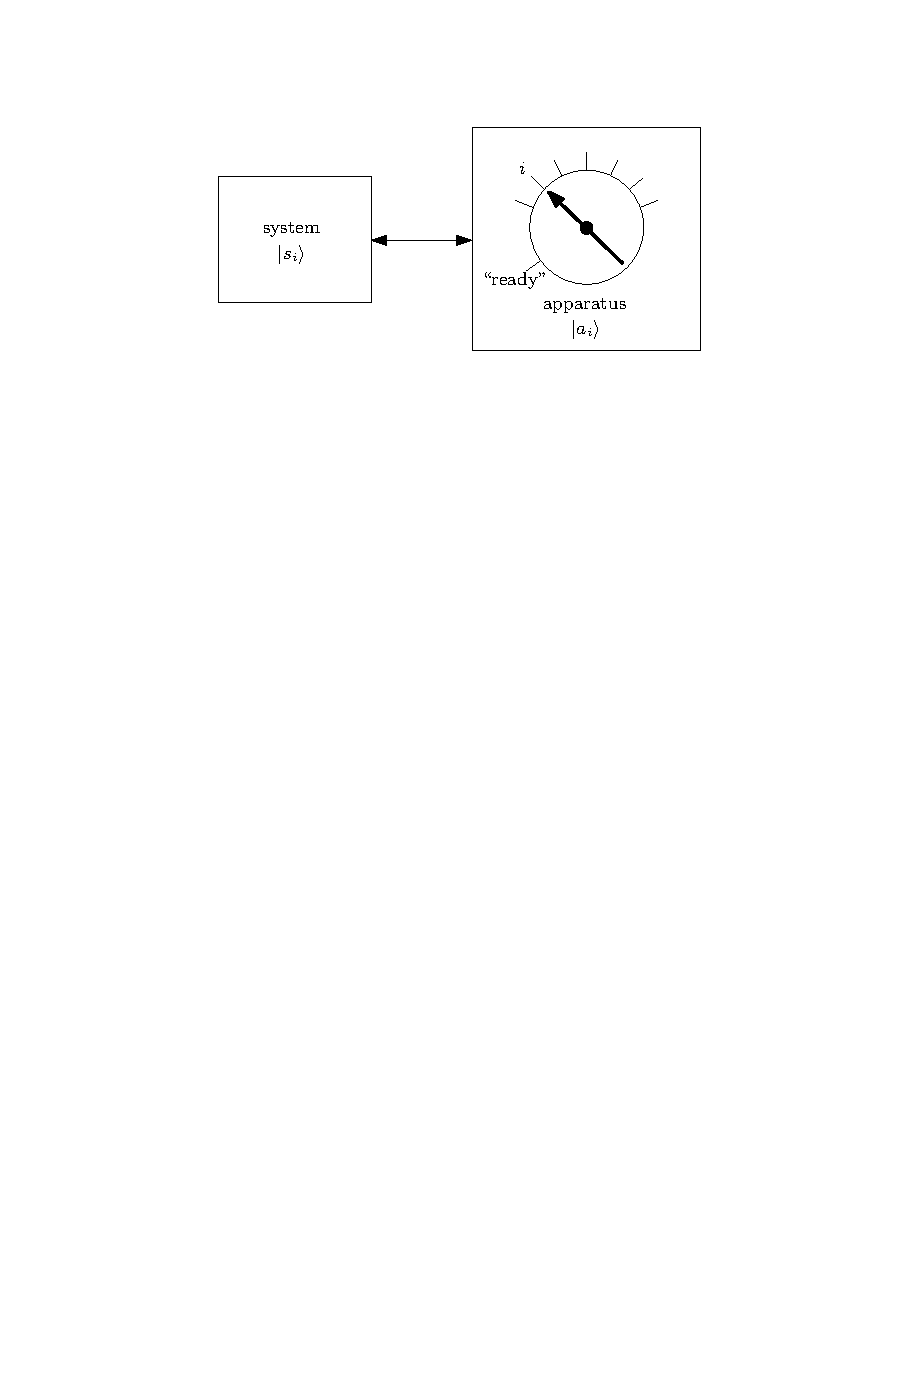
\includegraphics[width=.82\linewidth]{figures/ch02_fig04.pdf}\caption{理想的量子測定に対するvon Neumann方式。系と装置の両方を量子系として扱う。系と装置の相互作用は、系が状態$\lvert s_i\rangle$にあると、装置の指針が、目盛上の初期の「準備完了」位置から、装置の量子状態$\lvert a_i\rangle$で表される位置「$i$」へ動くようなものである。}\end{figure}

ここで重要な点に至る。これまでのところ、相互作用(2.52)は量子もつれを生じていない。系と装置の終状態は、なお分離可能である。しかし、系が初めに基底状態$\lvert s_i\rangle$の重ね合わせ
\begin{equation}\lvert\psi\rangle=\sum_i c_i\lvert s_i\rangle\tag{2.53}\end{equation}
にあるとき、何が起こるかを考えよう。この場合、Schrödinger方程式の線形性によれば、系と装置を合わせた$\mathcal{SA}$は、
\begin{equation}\lvert\psi\rangle\lvert a_r\rangle=\left(\sum_i c_i\lvert s_i\rangle\right)\lvert a_r\rangle\longrightarrow\lvert\Psi\rangle=\sum_i c_i\lvert s_i\rangle\lvert a_i\rangle\tag{2.54}\end{equation}
に従って発展する。この発展が、理想的なvon Neumann量子測定方式を表す。

式(2.54)の右辺を調べると、系と装置の組合せの終状態は、一般にもつれ状態で記述されることが分かる。すなわち、もはや系や装置に個別の状態ベクトルを帰属させられない。こうして量子もつれが力学的に作り出された。初めは系だけに存在した重ね合わせは、最終的な重ね合わせが系と装置の両方を含むという意味で、通常巨視的な装置の水準へ増幅された。

ここで決定的な難点は、式(2.54)が記述する力学的発展を、通常の意味の測定を表すと、どう見なすべきかが、まったく明らかでないことである。というのも、以下で論じる少なくとも二つの理由から、式(2.54)の右辺の終状態だけでは、測定が実際に完了したと直接に結論するのに不十分だからである。この事実を強調するため、方式(2.54)は、しばしば前測定と呼ばれる。

% 原文 p.53
\hypertarget{srcpage:53}{}\label{srcpage:53}
\subsubsectionlink{優先基底の問題}
第一の問題は、式(2.54)の右辺の最終的な複合状態の展開について、基底の曖昧さが存在することである。この状態は多くの異なる方法で表せるので、上のvon Neumann方式で測定されたはずの観測可能量は、この終状態によって一意には定義されない。実際、系$\mathcal S$を記述する任意の状態の組が与えられると、最終的な複合状態が式(2.54)の形を取るような、対応する装置状態の組が存在する。
\begin{equation}\lvert\psi\rangle\lvert a_r\rangle\longrightarrow\lvert\Psi\rangle=\sum_i c_i\lvert s_i\rangle\lvert a_i\rangle=\sum_i c_i'\lvert s_i'\rangle\lvert a_i'\rangle=\cdots.\tag{2.55}\end{equation}
しかし、基底選択のこの自由は、実際には二つの制約によって、ある程度制限される。第一に、通常は装置の状態$\lvert a_i\rangle$が互いに直交することを要求する。これにより、これらの状態が古典的に異なる測定結果に対応し、系の可能な状態$\lvert s_i\rangle$を確実に識別できる。第二に、装置状態の組$\lvert a_i\rangle$を任意に選ぶと、系の相対状態$\lvert s_i\rangle$は、互いに直交しないかもしれない。その場合、状態$\lvert s_i\rangle$に対応する、すなわち、それらを固有状態とする系の観測可能量は、Hermiteにならず、これは通常望ましくない性質である\footnote{ただし、非Hermiteな観測可能量は、先験的に禁止されているわけではなく、ある実験設定では現れる。たとえば量子光学では、コヒーレント状態を結果とする測定をしばしば行う。しかしコヒーレント状態は過完備な組をなし、したがってHermiteな観測可能量では表せない。Zurekの議論\cite{ref016}も参照。}。

これらを踏まえ、装置状態$\lvert a_i\rangle$は互いに直交し、すなわち$i\ne j$で$\langle a_i\vert a_j\rangle=0$と要求してよい。この場合、いわゆるSchmidt定理（後の2.15.1節）から、分解
\begin{equation}\lvert\Psi\rangle=\sum_i c_i\lvert s_i\rangle\lvert a_i\rangle,\qquad c_i\in\mathbb R,\quad\sum_i c_i^2=1\tag{2.56}\end{equation}
は、すべての係数$c_i$が互いに異なる限り、一意であることが従う。

% 原文 p.54
\hypertarget{srcpage:54}{}\label{srcpage:54}
係数についてのこの条件が成り立たないと、分解(2.56)が一般に一意ではないことを示す、単純な例を考えよう。系$\mathcal S$と装置$\mathcal A$が、どちらもスピン$1/2$粒子で表される量子力学的二状態系であり、基底状態$\lvert0_z\rangle$、$\lvert1_z\rangle$で記述されるとする。さらに、$\mathcal A$の状態$\lvert0_z\rangle_{\mathcal A}$、$\lvert1_z\rangle_{\mathcal A}$が、$\mathcal S$のスピン状態$\lvert0_z\rangle_{\mathcal S}$、$\lvert1_z\rangle_{\mathcal S}$の「指針」として働くとする。つまり、ここでのvon Neumann相互作用(2.52)は、
\begin{equation}\begin{split}\lvert0_z\rangle_{\mathcal S}\lvert\text{「準備完了」}\rangle_{\mathcal A}&\longrightarrow\lvert0_z\rangle_{\mathcal S}\lvert0_z\rangle_{\mathcal A},\\\lvert1_z\rangle_{\mathcal S}\lvert\text{「準備完了」}\rangle_{\mathcal A}&\longrightarrow\lvert1_z\rangle_{\mathcal S}\lvert1_z\rangle_{\mathcal A}\end{split}\tag{2.57}\end{equation}
という力学で記述される。系$\mathcal S$が重ね合わせ$(\lvert0_z\rangle_{\mathcal S}+\lvert1_z\rangle_{\mathcal S})/\sqrt2$から出発すると仮定すれば、式(2.57)とSchrödinger方程式の線形性から［式(2.54)も参照］、最終的な、もつれたスピンと装置の複合状態は、
\begin{equation}\lvert\Psi\rangle=\frac1{\sqrt2}(\lvert0_z\rangle_{\mathcal S}\lvert0_z\rangle_{\mathcal A}+\lvert1_z\rangle_{\mathcal S}\lvert1_z\rangle_{\mathcal A})\tag{2.58}\end{equation}
となる。式(2.35)を用いて、$z$スピン状態$\lvert0_z\rangle_i$、$\lvert1_z\rangle_i$（$i=\mathcal S,\mathcal A$）を、Pauliスピン演算子$\hat\sigma_x$の固有状態$\lvert0_x\rangle_i$、$\lvert1_x\rangle_i$で書き直そう。新しい基底$\{\lvert0_x\rangle_i,\lvert1_x\rangle_i\}$で表すと、状態(2.58)は
\begin{equation}\lvert\Psi\rangle=\frac1{\sqrt2}(\lvert0_x\rangle_{\mathcal S}\lvert0_x\rangle_{\mathcal A}+\lvert1_x\rangle_{\mathcal S}\lvert1_x\rangle_{\mathcal A})\tag{2.59}\end{equation}
となる。$\mathcal A$を、系$\mathcal S$のスピンの測定装置と見なしたことを思い出そう。式(2.58)、(2.59)は、装置$\mathcal A$が、$\mathcal S$の$z$スピン状態とも$x$スピン状態とも、一対一の相関を作ったことを意味する。von Neumann方式の精神に従い、その後の波動関数の収縮を仮定せず、系と装置の相関形成を完全な測定と解釈すると、この状況は次を意味するように見える。$\mathcal A$が$\mathcal S$の$z$軸方向のスピンを測定した時点で［終状態(2.58)］、$\mathcal S$の$x$軸方向のスピンも測定したと見なせる。後者の「測定」は、式(2.58)の同値な形(2.59)で表される。

したがって装置$\mathcal A$は、系の二つの非可換な観測可能量、すなわち$\hat\sigma_x$と$\hat\sigma_z$を同時に測定したように見え、量子力学の法則に反するように思われる。さらに、状態(2.58)は、実際には任意の軸に沿ったスピン$1/2$の基底を用いて、無限通りの同値な方法で書き直せると容易に示せる。したがって、装置$\mathcal A$が、式(2.58)の型の相関の形成というvon Neumannの意味で、$\mathcal S$の$z$軸方向のスピンを「測定」した時点で、他のすべての空間方向のスピンも「測定」したように見える。

非可換な観測可能量の組を同時に測定するこの状況は、量子力学で禁止されるだけでなく、測定装置はごく特定の量だけを測定するよう設計されているという経験にも反する。この例では、装置$\mathcal A$をStern--Gerlach装置（2.2.2節）として実現でき、状態$\lvert0_z\rangle_{\mathcal A}$、$\lvert1_z\rangle_{\mathcal A}$は、$z$軸方向に磁場を向けた装置を通る、分離した二つの経路に対応し、それによって系$\mathcal S$のスピン状態$\lvert0_z\rangle_{\mathcal S}$、$\lvert1_z\rangle_{\mathcal S}$を区別する。したがって、このStern--Gerlach装置は、$z$軸方向だけのスピンを測り、他の軸方向は測らないように設定されている。$z$と異なる軸に沿って測定するには、磁場を物理的に回転させる必要があり、物理的に異なる設定に対応する。

% 原文 p.55
\hypertarget{srcpage:55}{}\label{srcpage:55}
このような「優先観測可能量」、あるいは「優先基底」の存在は、von Neumann測定で到達する、系と装置の終状態では説明されない。見たように、この状態の形は一般に、量子的相関の形成を介して装置が記録する系の観測可能量を一意には固定しない。この優先基底の問題を、波動関数収縮の問題、およびそれと密接に関係する結果の問題（後の2.5.4節）から初めて明瞭に切り離したのはZurek\cite{ref008}であり、量子測定のいかなる説明でも優先基底の問題が果たす、独立した重要な役割を強調した。可能な結果の集合が明確に定義されていなければ、特定の結果を問うことさえ意味を持たないので、結果の問題が役割を持つ以前に、この優先基底の問題を解く必要がある。

Zurekはまた\cite{ref008,ref009}、優先基底の問題が、量子測定という狭い文脈をはるかに超えて、量子から古典への移行の問題で中心的役割を果たすことを認識した。ここでは、なぜ系、特に巨視的な系を、重ね合わせ原理が原理上許す物理量の、ごく小さな部分集合でしか知覚しないのか、という核心的な問いに出会う。最も顕著な例として、巨視的な系は常に、位置の重ね合わせではなく、確定した空間位置に見いだされる。何が位置を優先される量として選び出すのか。Zeh\cite{ref004}が最初に示唆し、Zurek\cite{ref008,ref009}が詳細に述べたように、これらに答え、優先基底の問題を克服するには、系と装置を、環境と相互作用する開いた量子系として考えなければならない。この方法を2.8節で詳しく論じる。

% 原文 p.55（後半）


\subsubsectionlink{干渉が観測されない問題}
多くの実験では、ある基底の成分状態の量子的重ね合わせが存在することを示す干渉模様を観測できる（2.2.2節）。しかし、より大きな尺度に進むと、そのような干渉模様は通常、消失する。たとえば電子などの微視的粒子で二重スリット実験を行うと、遠方の検出スクリーン上に干渉縞が現れる（第6章の図6.6）。しかし原子や分子で実験すると、干渉模様は普通、急速に消えてしまう。

% 原文 p.56
\hypertarget{srcpage:56}{}\label{srcpage:56}
従来の教科書の説明では、二重スリット実験で中間的・巨視的な物体の干渉模様が観測できないことを、古典的な光波の干渉との類似により説明するのが普通だった。後者では、干渉模様を観測するためには、回折を起こすスリットの間隔が、光の波長程度でなければならないことが、基礎光学でよく知られている。そして同じ議論を、物質による二重スリット実験という量子的場合に適用する。原子などの粒子のde Broglie波長はきわめて短いので、粒子の波長と同程度の幅と間隔を持つスリットを作るのは、実際には不可能である。この見方では、質量を持つ粒子の干渉模様を観測できないのは、粒子の量子的性質を引き出すのを妨げる、実験装置の不十分な「分解能」に由来する。

しかし、これは事情の一部にすぎない。たとえば、二重スリット実験と精神的には似ているが、微視的なスリットを作る必要という障害を避ける実験設定では、中間的な大きさの分子の空間干渉模様を観測できる（実験の詳細は6.2節）。それでも、回折過程に関係しない実験パラメータ、たとえば回折される分子の周囲の空気密度を変えると、干渉模様が減衰する。したがって、実験の回折段階が、干渉模様として観測できる空間的重ね合わせの生成を明らかに許していても、その模様を観測するのを妨げる、別の因子がある。このことは、「干渉を見る」難しさが、重ね合わせをそもそも生成するという問題だけでは説明できないことを、明瞭に示す。

さらに、さまざまな物理系に関する干渉実験の中には、物質の回折実験という分類にまったく入らないものも多い。たとえば、先に簡単に触れたように、逆向きに流れる電流の重ね合わせを作れる実験がある。これは、電流が二方向の間を往復して振動するという形で、時間的な干渉模様を生むはずである（こうした実験は6.3節で詳しく述べる）。それでも、実験条件が重ね合わせ状態の生成を許しているにもかかわらず、干渉を観測できないことが多く、少なくとも、きわめて精密に調整された実験条件が必要になる。この問題を、古典的な光波と量子的な「確率波」の回折の単純な類似で説明できないのは、明らかである。

ましてvon Neumann測定方式の終状態(2.54)からは、巨視的測定装置を含む重ね合わせが、自然界に遍在するはずだと従う。それなら、なぜ周囲の日常世界で、装置の異なる指針位置の間の干渉を観測しないように見えるのか。von Neumann方式は、重ね合わせが微視的な水準から巨視的な水準へ容易に増幅されるはずだと明瞭に示すのに、なぜ中間的・巨視的領域で、何らかの干渉効果を観測するのはそれほど難しいのか。

% 原文 p.57
\hypertarget{srcpage:57}{}\label{srcpage:57}
本質的には、これが干渉の非観測性の問題である。間もなく、デコヒーレンスが、干渉模様の観測される減衰、あるいはそもそもその模様を実験的にまったく観測できないことを、環境自由度との相互作用の結果として説明することにより、この問題への非常に洗練された一般的な答えを与えるのを見る。

\subsubsectionlink{結果の問題}
経験によれば、あらゆる測定は、測定量の確定した値をもたらす。実際、「結果」「値」「量」などの語の定義自体が、この確定性に本質的に依拠する。他方、von Neumann方式で得られる終状態(2.54)は、系と装置の状態の重ね合わせを表す。2.2.1節の議論から、そのような重ね合わせは、系と装置の組合せが実際には成分状態$\lvert s_i\rangle\lvert a_i\rangle$の一つだけにあるが、どれかを私たちが知らないという、状態の古典的集団とは根本的に異なることが分かっている（上の2.4.2節の分析も参照）。したがって、何らかの収縮機構のような追加の物理過程を与えるか、そのような重ね合わせに適切な解釈を与えない限り、最終的な複合状態が与えられたとき、実際の測定の結果として観測される確定した指針位置を、どう説明するかは明らかでない。

この問題はさらに、異なる二つの側面に分けられる。第一に、測定の完了時に、なぜ装置の指針を、異なる指針位置$\lvert a_i\rangle$の重ね合わせとして知覚しないのかという問いに直面する。そもそも、そのような重ね合わせを観測することが何を意味するとしても、なぜ測定には結果があるように見えるのか。第二に、何が特定の結果を「選ぶ」のかを問える。すなわち、測定を実現する実験の各実行で、なぜ他の可能な状態$\lvert a_{j\ne i}\rangle$ではなく、特定の指針位置$i$、したがって特定の指針状態$\lvert a_i\rangle$を観測するのか。両方を合わせて、結果の問題と呼ぶことにする。

結果の問題は、第1章で述べたSchrödingerの猫のパラドックスの直接の基礎にある。その第一の部分が、最終的な原子と猫の複合状態は、古典的には互いに排他的な状態の重ね合わせで記述されると、量子力学が予言するように見えることに関わるのを、思い出そう。簡単のため、ここではハンマーと毒を明示的には議論に含めない。この部分は単に、原子と猫の間のvon Neumann型の、測定に似た相互作用から生じると理解できる。ここで原子は微視的系$\mathcal S$に対応し、猫は、その生死が原子の状態の指標、すなわち「指針」であるという意味で、巨視的装置を表す。式(2.52)に従えば、「測定」方式は次となる。

% 原文 p.58
\hypertarget{srcpage:58}{}\label{srcpage:58}
\begin{align}
\lvert\text{「原子は未崩壊」}\rangle\lvert c_r\rangle&\longrightarrow\lvert\text{「原子は未崩壊」}\rangle\lvert\text{「猫は生存」}\rangle,\tag{2.60a}\\
\lvert\text{「原子は崩壊」}\rangle\lvert c_r\rangle&\longrightarrow\lvert\text{「原子は崩壊」}\rangle\lvert\text{「猫は死亡」}\rangle.\tag{2.60b}
\end{align}
ここで$\lvert c_r\rangle$は猫の初期状態である。量子力学によれば、不安定な原子は常に、原子が崩壊した状態と未崩壊の状態の重ね合わせ、
\begin{equation}\lvert\psi\rangle=\alpha\lvert\text{「原子は未崩壊」}\rangle+\beta\lvert\text{「原子は崩壊」}\rangle\tag{2.61}\end{equation}
で記述される。ここで$\alpha$と$\beta$は、$\lvert\alpha\rvert^2+\lvert\beta\rvert^2=1$を満たす時間依存の係数である。一般的なvon Neumann方式(2.54)とまったく同じく、Schrödinger方程式が線形であることによって、原子と猫の最終的な複合系は、次の形のもつれ状態で記述される。
\begin{equation}\begin{split}\lvert\psi\rangle\lvert c_r\rangle\longrightarrow{}&\alpha\lvert\text{「原子は未崩壊」}\rangle\lvert\text{「猫は生存」}\rangle\\&+\beta\lvert\text{「原子は崩壊」}\rangle\lvert\text{「猫は死亡」}\rangle.\end{split}\tag{2.62}\end{equation}
もはや猫には個別の量子状態を帰属させられず、そのため「猫は生きても死んでもいない」と見える。式(2.62)の右辺の終状態が記述する状況は、しばしばこのように解釈される\footnote{実際、このような状況は、単に私たちの経験の一部でないので、言葉で適切に表すのは難しい。}。ただし「生」と「死」の状態の重ね合わせで記述されるのは、猫自体ではないことに注意しよう。むしろ原子と猫の複合状態が、原子と猫の状態の重ね合わせで表されるのである。ここでもハンマーと毒は省略している。

第1章で説明したように、Schrödingerの猫のパラドックスの第二の部分は、少なくとも量子力学の標準解釈（8.1節）によれば、箱を開けて内容を直接観測し、仮定された「波動関数の収縮」を起こすまで、重ね合わせ(2.62)が存続することに関わる。これは、どうして、またなぜ猫の運命を外部観測者の介入（von Neumannの「erster Eingriff」）に委ねられるのかという問いを生む。もちろん、これは本質的に結果の問題そのものである。重ね合わせ状態(2.62)が与えられたとき、猫の確定した状態、すなわち生きているか死んでいるかの一方にある猫を、観測者が経験することを、どう説明できるだろうか。

結果の問題を解消すること、すなわち、重ね合わせ原理の最重要かつ実験で確認された役割と、測定で単一の確定した結果が観測されることとの見かけ上の矛盾を解くことは、量子力学のあらゆる解釈の中心的動機の一つであった。量子力学の標準的、または「正統的」解釈（詳細は8.1節）は、物理量に対応する観測可能量が確定した値を持つのは、系がその観測可能量の固有状態にある場合、かつその場合に限ると規定する。他方、系がその固有状態の重ね合わせで記述される場合には、系の物理状態が、その観測可能量の何らかの確定した値を持つと語ること自体、無意味と見なされる。

% 原文 p.59
\hypertarget{srcpage:59}{}\label{srcpage:59}
この正統的量子力学の規則は、しばしば固有値と固有状態の結び付き、あるいは、より的確に値と固有状態の結び付きと呼ばれる。

しかし、固有値と固有状態の結び付きは、量子力学の構造からも、いかなる経験的制約からも要請されない\cite{ref068}。さらに「厳密な」固有値と固有状態の結び付きという概念は、それ自体の難点を生む。たとえば測定の結果は、典型的には位置空間に局在した指針で記録される。しかし指針は、決して完全には局在しない。すなわち、位置演算子の厳密な固有状態では記述できない。そのような固有状態は、無限の運動量の広がり、したがって系に含まれる無限のエネルギーに対応するため、非物理的だからである。したがって異なる指針位置に対応する状態は、厳密には互いに直交できない。

そのため、観測可能量とその厳密な固有状態の存在に基づき、固有値と固有状態の結び付きを通じて帰属させられる、古典的な「値」という概念は、しばしば弱められるか、完全に放棄されてきた。そのうえで、量子形式と測定概念をある仕方で再解釈するか、量子力学自体に実際の修正を導入する。前者に属する相対状態解釈と様相解釈は、von Neumann方式(2.54)に現れる最終的な系と装置の複合状態を、量子状態が重ね合わせの形を取るにもかかわらず、結果の存在、または少なくともその主観的知覚を説明するように解釈しようとする。後者に属する物理的収縮模型は（2.2.3節ですでに簡単に触れた）、Schrödinger発展のユニタリ性を破り、波動関数を一成分へ「客観的に」還元する、自然界の何らかの根本的機構の存在を仮定する。これらのさまざまな解釈と、デコヒーレンスとの関係は、第8章でさらに詳しく論じる。

一般に、結果の問題は、確率的理論において、何が特定の結果を現実化するのかという問いに根差す。古典的な確率理論では、この問いに答えることは、少なくとも原理上は難しくない。そこでは、確率の概念は、ある問題の扱いを簡単にする、便利な粗視化手順の帰結にすぎない。しかし物理系の根本的な水準では、具体的な結果は、その基礎にある決定論的な物理法則によって完全に指定される。それが、たとえば何十億個もの原子からなる系について、実際にはどれほど複雑に見えるとしても、である。したがって原理上、古典物理学から確率的な側面をすべて取り除ける。

% 原文 p.60
\hypertarget{srcpage:60}{}\label{srcpage:60}
これに対し、2.1節で詳しく論じたように、量子力学は、本質的に確率的な性格を持つように見える。純粋量子状態は、すでに系の物理状態の完全な記述を表し、その発展は決定論的なSchrödinger方程式で与えられる。それでも、各測定時にどの具体的結果が実現するかを決定する根本的機構は存在しない。したがって、結果の問題は量子力学自体にとって根本的である。そのため、この問題の解決にデコヒーレンスが寄与することに期待できる最大の希望は、なぜ測定で、結果の重ね合わせではなく、可能な結果の一つだけが実際に観測されるかを説明することである。しかし、von Neumannの終状態(2.54)では、いかなる可能な結果も形式的にはまったく特別扱いされないのに、なぜ他の結果ではなく特定の結果が観測者に現れるのかという問いは、デコヒーレンスの範囲外にある、量子力学の解釈の根本的問題に属する。第8章で再びこの話題に戻る。

% 原文 p.60（後半）


\subsectionlink{経路情報と環境による監視}
デコヒーレンスに関係する量子力学の形式と解釈の主要要素、すなわち量子状態、重ね合わせ原理、量子もつれ、密度行列、および測定問題を示したので、ついに実際の関心の対象、デコヒーレンスに取り組むための準備が整った。まず、よく知られた二重スリット実験を再訪することによって、この課題に取り組む。この実験は、デコヒーレンスの基本的機構を、非常に直観的で分かりやすく示すだろう。

\subsubsectionlink{二重スリット実験、経路情報、および相補性}
通常の二重スリット装置を描いた図2.2を振り返ろう。左から近づく電子などの粒子が、二つのスリットのあるスクリーンに入射する。スリットを通過した後、遠方の検出スクリーンに当たり、消えない斑点を残す。量子力学が予言し、実験が確認するように、二つの異なる極限的な領域がある（2.2.2節の議論も参照）。
\begin{enumerate}
\item 「波」の状況（図2.2の右）。各粒子がどちらのスリットを通ったかを測定しなければ、検出スクリーンの位置で観測される粒子密度は、$\varrho(x)=\frac12\lvert\psi_1(x)+\psi_2(x)\rvert^2$という干渉模様に対応する。これは、それぞれスリット1、2の通過を表す部分波$\psi_1(x)$、$\psi_2(x)$の、量子力学的重ね合わせに対応する確率密度である。
\item 「粒子」の状況（図2.2の中央）。一方のスリットに検出器を置き、粒子がそのスリットを通ったかを調べると、干渉模様は消える。遠方のスクリーンの密度模様は、スリット1を通ったすべての粒子が作る模様（スリット2を覆ったときに得る模様）と、スリット2を通ったすべての粒子が作る模様を、古典的に足し合わせたもの、$\varrho(x)=\frac12\lvert\psi_1(x)\rvert^2+\frac12\lvert\psi_2(x)\rvert^2$に等しい。
\end{enumerate}

% 原文 p.61
\hypertarget{srcpage:61}{}\label{srcpage:61}
第二の場合、すなわち「粒子」の状況に対する標準的説明は、次のとおりである。量子力学によれば、スリットの位置での粒子の状態は、部分波$\psi_1(x)$、$\psi_2(x)$の重ね合わせ$\Psi(x)=(\psi_1(x)+\psi_2(x))/\sqrt2$で与えられる。この重ね合わせは、両スリットを含む領域に空間的に広がっている。一方のスリットで粒子の位置を測定し、実際にそのスリットに粒子が存在すると分かれば、$\Psi(x)$を対応する空間領域に局在化する。すなわち、$\psi_1(x)$と$\psi_2(x)$は、スリットの位置では重なりが無視できるため、量子力学の標準的な収縮公準を用いて、測定が重ね合わせ$\Psi(x)$を、成分状態$\psi_1(x)$、$\psi_2(x)$の一方へ収縮させたと言える。したがって、部分波間の干渉はもはや得られず、遠方のスクリーンの干渉模様は消える。

言い換えれば、粒子が二つのスリットのどちらを通ったかを見るために、粒子の経路情報（Welcher-Weg情報）を得ようとするたびに、空間的干渉という量子的性質を示す能力を、どうしても破壊してしまうように見える。これは、両スリットを同時に通るという反直観的な事態を記述するように見える、二つの経路の量子力学的重ね合わせを、理解しようとするたびに起こる。したがってNiels Bohrの有名な用語\cite{ref070}を使えば、経路情報（「粒子」の側面）と干渉（「波」の側面）の間には相補性がある。実験設定、すなわち粒子の経路を測定するかどうかに応じて、「粒子的」または「波的」な振る舞いのどちらかを観測するように見える。この「波と粒子の二重性」は量子論の基礎とされ、物理学者と物理哲学者の双方による、数え切れない議論の対象となってきた。

相補性原理とその適用は、1927年にBrusselsで開かれた第5回Solvay会議での、EinsteinとBohrの有名な論争の主題であった\cite{ref071}。Einsteinは会議で、標準的な二重スリット装置についての次の思考実験をBohrに突き付けた。運動量保存則によれば、粒子が上側、または下側のスリットを通ると、スリットを持つスクリーンには、上向き、または下向きの反跳が生じるはずだと論じた。スクリーンの反跳方向を測定できるとしよう（図2.5）。この測定により、少なくとも原理上、粒子の経路を推論でき、経路情報が得られる。Einsteinは、干渉模様はスリットから出る二つの波束の干渉だけによるので、スクリーンの段階で反跳方向を決めても、その後の発展には影響しないはずであり、したがって干渉模様は観測されるはずだと主張した。これはBohrの相補性原理と矛盾するように見える。

% 原文 p.62
\hypertarget{srcpage:62}{}\label{srcpage:62}
\begin{figure}[htbp]\centering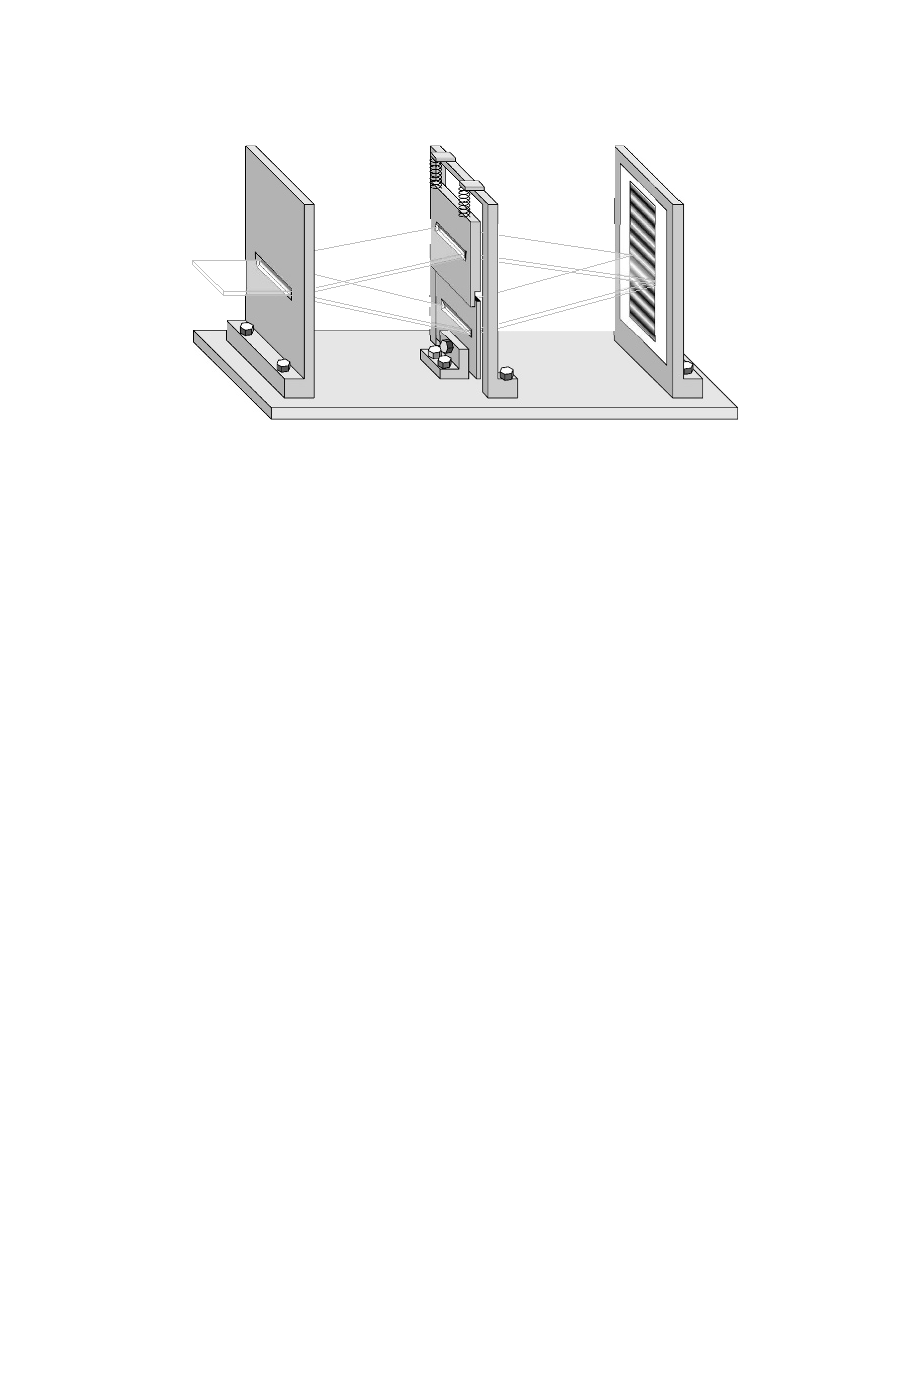
\includegraphics[width=.9\linewidth]{figures/ch02_fig05.pdf}\caption{二重スリット実験で経路情報を得る、Einsteinの思考実験。左のコリメート用スリットを出た粒子は、中央の二重スリットを通り、右の検出スクリーンに記録される。粒子がスリットを通過するとスリットに運動量が伝わり、原理上は、スリットのあるスクリーンの反跳として測定できるはずである。下のスリットは固定し、上のスリットはばねで吊るす。したがって、上のスリットを通る粒子は、吊るされたスリットに小さな振動運動を引き起こし、それを少なくとも原理上は検出できるため、粒子がどちらのスリットを通ったかを推論できる。図はBohrの原図\cite{ref072}に基づき、Macmillan Publishers Ltdの許可により、Nature、copyright 2001の文献\cite{ref073}から転載した。}\end{figure}

Bohrは、この挑戦に次のように応じた。単一粒子がスリットに与える反跳は、通常きわめて小さい。この微小な運動量変化を分解するには、スリットのあるスクリーンの初期運動量を、検出しようとする反跳と少なくとも同じくらい小さな範囲内で知っていなければならない。不確定性原理によれば、スクリーンの運動量をそのような高精度で測定することは、スクリーン位置の大きな不確定性を意味する。そこでBohrは、入射粒子がスリットに到達するより前の、スクリーンの初期運動量の測定だけで、その結果生じる位置の不確定性が、検出スクリーン上の干渉縞の位置に可能な幅を与え、その幅が、干渉縞の特徴的間隔程度になることを示した。したがって、その位置の幅にわたって干渉模様を平均すると、模様は「洗い流される」。ある可能な位置の模様での極大の位置が、別のスクリーン位置に対する模様での極小と重なるので、正味の干渉模様は消える。

% 原文 p.63
\hypertarget{srcpage:63}{}\label{srcpage:63}
したがってBohrの中心的主張は、経路情報の獲得は、不可避な系の擾乱を伴う、というものである。これは、スクリーンの反跳を測って経路情報を得るBohr--Einsteinの例では、実際に正しい。しかし、WoottersとZurek\cite{ref074}が最初に示し、ScullyとDrühl\cite{ref075}がさらに調べたように、ある状況では、粒子の空間波動関数を有意に変化させずに経路情報を集めることもできる。その場合、Bohrが指摘した位置と運動量の不確定性原理の効果は軽減される。次節でこれを論じる。

\subsubsectionlink{量子もつれによる二重スリット実験の記述}
これまで、経路情報の獲得と干渉模様の観測の相補性を、不連続な二者択一の区別として導入した。しかし、たとえば粒子がどちらのスリットを通ったかを不正確に測定して、経路情報の一部だけを集めれば、干渉模様を一部残せないだろうか\cite{ref074}。

この問いの答えは肯定的である。しかし、量子力学のこの特徴を論じ説明するには、上で用いた波動関数の収縮による記述は、もはや適切でない。公準によれば収縮は、不連続で不可逆な過程であり、経路情報量と干渉の程度の、滑らかで可逆な変化を説明できない。代わりに、von Neumann測定方式（2.5.1節）と量子もつれによる、純粋に量子力学的な説明を進める。この記述は、その後、環境が経路検出器の役割を担う、デコヒーレンス過程の記述の基礎にもなる。二重スリット実験での干渉の観測可能性と量子もつれのつながりは、WoottersとZurek\cite{ref074}が初めて論じた。

スリット1、2の通過に対応する粒子の量子状態を、それぞれ$\lvert\psi_1\rangle$、$\lvert\psi_2\rangle$と書こう。前と同じく両方のスリットに検出器を置き、ともに初めは「準備完了」状態にする。スリット2を覆い、粒子源をスリット1のすぐ後ろに置いて粒子が必ずこのスリットを通るようにすれば、粒子を、たとえば状態$\lvert\psi_1\rangle$に準備できる。するとスリット1の検出器は作動し、スリット2の検出器は、作動しない「準備完了」状態にとどまる。以下では、二つの個別検出器を合わせて「検出器」と呼ぶ。この複合検出器の共同の「準備完了」状態を$\lvert\text{「準備完了」}\rangle$、上記のように状態$\lvert\psi_1\rangle$を準備した後の、この検出器系の量子状態を$\lvert1\rangle$と書き、粒子がスリット1を通ったことを示す。この場合、粒子と検出器の複合系の状態発展は、次の形になる。

% 原文 p.64
\hypertarget{srcpage:64}{}\label{srcpage:64}
\begin{equation}\lvert\psi_1\rangle\lvert\text{「準備完了」}\rangle\longrightarrow\lvert\psi_1\rangle\lvert1\rangle.\tag{2.63}\end{equation}
スリットの役割を入れ替えて同じ議論をすると、
\begin{equation}\lvert\psi_2\rangle\lvert\text{「準備完了」}\rangle\longrightarrow\lvert\psi_2\rangle\lvert2\rangle\tag{2.64}\end{equation}
を得る。式(2.63)、(2.64)は、測定相互作用の一般的記述(2.52)に対応する。

両スリットが開いていれば、粒子は二つの成分$\lvert\psi_1\rangle$、$\lvert\psi_2\rangle$の重ね合わせ$\lvert\psi\rangle=(\lvert\psi_1\rangle+\lvert\psi_2\rangle)/\sqrt2$で記述されなければならない。そのため式(2.63)、(2.64)から、von Neumann型(2.54)の力学的発展が得られ、粒子と検出器のもつれた複合状態に至る。
\begin{equation}\frac1{\sqrt2}(\lvert\psi_1\rangle+\lvert\psi_2\rangle)\lvert\text{「準備完了」}\rangle\longrightarrow\frac1{\sqrt2}(\lvert\psi_1\rangle\lvert1\rangle+\lvert\psi_2\rangle\lvert2\rangle).\tag{2.65}\end{equation}
ここでも、検出器状態$\lvert1\rangle$、$\lvert2\rangle$は、系の相対状態$\lvert\psi_1\rangle$、$\lvert\psi_2\rangle$の「指針」として働く。

いま粒子に測定を行うことにより、たとえば位置測定に対応する、検出スクリーンへの衝突によって、粒子について何が分かるだろうか。2.4.6節から分かるように、関心のある量は粒子の縮約密度行列であり、式(2.65)の右辺の純粋状態に対しては、式(2.49)より
\begin{equation}\begin{split}\hat\rho_{\mathrm{particle}}=\frac12\{&\lvert\psi_1\rangle\langle\psi_1\rvert+\lvert\psi_2\rangle\langle\psi_2\rvert\\&+\lvert\psi_1\rangle\langle\psi_2\rvert\langle2\vert1\rangle+\lvert\psi_2\rangle\langle\psi_1\rvert\langle1\vert2\rangle\}.\end{split}\tag{2.66}\end{equation}
この密度行列に対応する、検出スクリーンでの粒子密度$\varrho(x)$は、
\begin{equation}\begin{split}\varrho(x)&\equiv\rho_{\mathrm{particle}}(x,x)\equiv\langle x\rvert\hat\rho_{\mathrm{particle}}\lvert x\rangle\\&=\frac12\lvert\psi_1(x)\rvert^2+\frac12\lvert\psi_2(x)\rvert^2+\operatorname{Re}\{\psi_1(x)\psi_2^*(x)\langle2\vert1\rangle\}\end{split}\tag{2.67}\end{equation}
で与えられる。ここで$\psi_i(x)=\langle x\vert\psi_i\rangle$（$i=1,2$）である。最後の項は、よく知られた干渉模様を記述し、その可視度は重なり$\langle2\vert1\rangle$で定量化されることが分かる。これは、先の2.4.6節の議論に直接につながる。

特に、検出器状態$\lvert1\rangle$、$\lvert2\rangle$が完全に識別可能な極限、$\langle2\vert1\rangle=0$は、「粒子」の領域に対応する。
\begin{equation}\varrho(x)=\frac12\lvert\psi_1(x)\rvert^2+\frac12\lvert\psi_2(x)\rvert^2.\tag{2.68}\end{equation}
逆に、$\lvert1\rangle$、$\lvert2\rangle$が粒子の経路をまったく分解できず、位相因子を無視して$\langle2\vert1\rangle=1$なら、完全な干渉模様という「波」の状況が当てはまる。

% 原文 p.65
\hypertarget{srcpage:65}{}\label{srcpage:65}
\begin{equation}\varrho(x)=\frac12\lvert\psi_1(x)\rvert^2+\frac12\lvert\psi_2(x)\rvert^2+\operatorname{Re}\{\psi_1(x)\psi_2^*(x)\}.\tag{2.69}\end{equation}
検出器が完全ではない一部の経路情報を得る状況は、二つの検出器状態$\lvert1\rangle$、$\lvert2\rangle$の重なりが、非零だが1未満であることで、形式的に表される。式(2.66)から、その場合には干渉模様を観測できるが、重なり$\langle2\vert1\rangle$が小さくなる、すなわち検出器状態$\lvert1\rangle$、$\lvert2\rangle$が識別しやすくなり、検出器が得る経路情報量が増すにつれて、模様は次第に減衰することが分かる。

したがって、経路情報が不完全である限り、干渉模様を観測することと、スリットを通る粒子の経路について、いくらかの情報を得ることは、実際に同時に可能であると示された。検出器の得た情報が、粒子の通った経路を確実に推論できるだけ十分になるとすぐ、干渉模様は消える。WoottersとZurek\cite{ref074}は、経路情報と干渉の、この根本的な相反関係、したがって相補性と量子もつれの密接な関係を分析し、目に見える干渉模様を保ちながら、かなり大量の経路情報を得られることを指摘した。具体的には、経路について90\%の確実さを得ても、干渉模様には約50\%のコントラストが残ることを示した。

まとめると、干渉模様を観測できる程度は、関心のある物体ともつれた、何らかの系に符号化されている、利用可能な経路情報によって決まるだけであり、その量は、必ずしも物体自体の空間波動関数に影響せずに変えられる。したがって相補性は、量子もつれの帰結と見なせる。

% 原文 p.65（後半）


\subsubsectionlink{経路を監視するものとしての環境}
この本を考えよう。本は、空気分子、可視光や熱の光子、さらには宇宙のニュートリノや放射性の背景放射からなる、大きな環境に浸っている。毎秒、膨大な数のこれらの粒子が本に衝突し、散乱される。各衝突は、本の位置と向きに応じて、粒子をある程度偏向させる。ある一個の空気分子に注目しよう。それは、ある初期位置から一定の速度で出発し、本に散乱され、入射経路に対して一定の角度だけ曲がった軌道に沿って飛び去る。

本の向きが違う角度だったとしよう。その場合、空気分子は一般に、最初の場合とは異なる方向へ飛び去る。したがって、散乱された分子のこの二つの異なる経路によって、本に二つの異なる空間的向きが存在することを区別できる。言い換えれば、散乱粒子である空気分子は、ここでは本である散乱物体の位置と向きについての情報を持ち去る。

% 原文 p.66
\hypertarget{srcpage:66}{}\label{srcpage:66}
すでになじみ深い用語を使えば、それらは系についての経路情報を符号化する。ここで、以後の本文でも同じだが、「経路情報」という語は、より一般的に「どの状態かという情報」の意味に理解してほしい。前者の用語は、関心のある情報がスリットを通る粒子の経路に関わる、二重スリット実験の例によって、歴史的に動機付けられている。それでも、実際には粒子の軌道に関する情報でない場合にも、定着した用語「経路情報」をしばしば使う。

本に衝突する一個の空気分子は、本の向きについて、多くの情報を持ち去らないかもしれない。結局、散乱が起こるのは、本の大きさに比べて微小な領域だけである。しかし上に述べたように、どの瞬間にも、何百万個もの分子が本の表面に散乱されている。これらすべての分子を合わせたものに符号化される経路情報、あるいは、より適切には「どの向きかという情報」は、本の二つの異なる位置と向きがとても似ている場合でも、それらを識別するのに、確かに十分であろう。

この議論を、量子形式によって模式的に表そう。1秒間に本で散乱される$N$個すべての粒子に注目する。衝突前の$N$個すべての環境粒子の量子状態を$\lvert E_0\rangle$で表す。衝突後、各粒子は何らかの速度で、ある軌道に沿って飛び去る。本の向きが別であれば、粒子は少し異なる方向へ散乱されるかもしれない。$N$個すべての粒子が、本に散乱されたとする。本の向きに応じて、散乱後の環境状態を、それぞれ$\lvert E_1\rangle$、$\lvert E_2\rangle$と書く。

上の議論によれば、この二つの状態に含まれる情報は、本の二つの向きを識別するのに十分なので、これらは明らかに区別できる。したがって、$\lvert E_1\rangle$と$\lvert E_2\rangle$の重なりは、無視できるほど小さい\footnote{$\lvert E_1\rangle$、$\lvert E_2\rangle$を、個々の分子に属する状態の積、$\lvert E_1\rangle=\prod_{i=1}^N\lvert e_1\rangle_i$、$\lvert E_2\rangle=\prod_{i=1}^N\lvert e_2\rangle_i$と考えられる。各分子状態の対の重なりは1に近く、$(\langle e_1\vert e_2\rangle)_i\approx1$であるが、そのような個別状態を多数$N$個掛け合わせた積状態$\lvert E_1\rangle$、$\lvert E_2\rangle$は、近似的に直交する。}。前の2.6.2節で導入した経路情報の形式とのつながりが、明瞭に分かる。環境状態$\lvert E_1\rangle$、$\lvert E_2\rangle$は、単に経路検出器、ここでは向き検出器の状態に対応する。

重要なのは、このような環境の経路検出器が、自然界のあらゆる場所にあることである。どの物体も環境と相互作用し、環境は系のある物理的性質について情報を得る。本を高い真空度の中に置けば、空気分子をある程度遮蔽できるかもしれない。可視光の光子を遮断し、本を冷やして熱光子の影響も減らそうとできるかもしれない。それでも、次の第3章で見るように、他の源からの粒子が残り、系の位置を「測定」し続ける。系に対して、von Neumannの意味での実効的測定を連続的に行う、遍在する「測定装置」としての環境の、この決定的役割を、初めて明瞭に認識して論じたのは、1980年代初頭のZurekであった\cite{ref008,ref076}。

% 原文 p.67
\hypertarget{srcpage:67}{}\label{srcpage:67}
この監視過程に、いかなる人間の観測者も必要ないことを強調する。環境に符号化された経路情報を、原理上読み出せるという事実だけで、干渉模様が消え、粒子が「波としての性質を失う」のに十分である。これにより、2.1.3節ですでに引用した、Heisenbergの「粒子の軌道は、私たちがそれを観測するという行為によって作られる」\cite[p.~185]{ref042}という言葉に、より正確で、観測者に依存しない意味が与えられる。この実証主義的態度は、第1章で述べたEinsteinの有名な修辞的な問い、「月は私が見ているときにしか存在しないのか」\cite{ref003}に代表されるように、量子論に対する多くの批判を生んできた。

ここで、2.6.2節と同じ形式的議論を行える。系が、異なる二つの位置$x_1$、$x_2$のまわりへの局在に対応する量子状態$\lvert\psi_1\rangle$、$\lvert\psi_2\rangle$の、コヒーレントな重ね合わせで記述されるとしよう。二重スリット実験では、対応する位置空間の波動関数$\psi_1(x)$、$\psi_2(x)$は、スリットでの部分波を表す。環境粒子の散乱が起こる前、系と環境を合わせた状態は、積の形
\begin{equation}\lvert\psi\rangle\lvert E_0\rangle=\frac1{\sqrt2}(\lvert\psi_1\rangle+\lvert\psi_2\rangle)\lvert E_0\rangle\tag{2.70}\end{equation}
を持つ。上の議論に従い、系と環境の相互作用の力学は、
\begin{align}\lvert\psi_1\rangle\lvert E_0\rangle&\longrightarrow\lvert\psi_1\rangle\lvert E_1\rangle,\tag{2.71a}\\\lvert\psi_2\rangle\lvert E_0\rangle&\longrightarrow\lvert\psi_2\rangle\lvert E_2\rangle\tag{2.71b}\end{align}
で与えられる。すなわち、環境の状態は、系の状態に応じて$\lvert E_1\rangle$または$\lvert E_2\rangle$に発展する。するとSchrödinger方程式の線形性から、通常のvon Neumann発展
\begin{equation}\frac1{\sqrt2}(\lvert\psi_1\rangle+\lvert\psi_2\rangle)\lvert E_0\rangle\longrightarrow\frac1{\sqrt2}(\lvert\psi_1\rangle\lvert E_1\rangle+\lvert\psi_2\rangle\lvert E_2\rangle)\tag{2.72}\end{equation}
が従う。系の相対状態$\lvert\psi_1\rangle$、$\lvert\psi_2\rangle$は、経路情報を符号化する環境状態$\lvert E_1\rangle$、$\lvert E_2\rangle$ともつれた。初めは系だけに限られていた重ね合わせが、より大きな、系と環境の複合状態へ広がった。それに対応して、成分$\lvert\psi_1\rangle$、$\lvert\psi_2\rangle$間のコヒーレンスは、もはや系だけの性質ではなく、大域的な系と環境の状態の共有された性質となった。そのため、コヒーレンスが、環境を含むようになった「より大きな系の中へ非局在化した」\cite[p.~5]{ref077}と言うことが多い。式(2.72)で記述される、系と環境の力学的発展が、デコヒーレンス過程の基本的な形式的表現であり、その帰結を次に論じる。

% 原文 p.68
\hypertarget{srcpage:68}{}\label{srcpage:68}
\subsectionlink{デコヒーレンスと干渉の局所的減衰}
状態(2.72)における系の縮約密度行列$\hat\rho_{\mathrm{particle}}$は、式(2.49)、(2.66)より
\begin{equation}\begin{split}\hat\rho_{\mathrm{particle}}=\frac12\{&\lvert\psi_1\rangle\langle\psi_1\rvert+\lvert\psi_2\rangle\langle\psi_2\rvert\\&+\lvert\psi_1\rangle\langle\psi_2\rvert\langle E_2\vert E_1\rangle+\lvert\psi_2\rangle\langle\psi_1\rvert\langle E_1\vert E_2\rangle\}\end{split}\tag{2.73}\end{equation}
で与えられる。いつものように、最後の二項は成分状態$\lvert\psi_1\rangle$、$\lvert\psi_2\rangle$の間の干渉に対応する。環境が実際に十分な経路情報を記録したなら、最終的な環境状態$\lvert E_1\rangle$、$\lvert E_2\rangle$は近似的に直交し、$\langle E_2\vert E_1\rangle\approx0$になる。上の、空気分子が巨視的物体に1秒間にわたって散乱される例では、これは確かに成り立つ。そのとき、縮約密度行列(2.73)の干渉は抑制される。
\begin{equation}\hat\rho_{\mathrm{particle}}\approx\frac12\{\lvert\psi_1\rangle\langle\psi_1\rvert+\lvert\psi_2\rangle\langle\psi_2\rvert\}.\tag{2.74}\end{equation}
系と環境の両方を含む測定だけが、重ね合わせ状態(2.72)の成分間に存続するコヒーレンスを、明らかにしうる。しかし実際には、系と相互作用した多数の環境自由度のすべてを観測に含めることは不可能である。JoosとZeh\cite[p.~224]{ref007}は、この状況を「干渉項はなお存在するが、そこにはない」と端的にまとめた。すなわち、干渉項は、系と環境の重ね合わせ(2.72)という大域的水準には残るが、縮約密度行列(2.74)で記述される系の局所的水準では、観測不能となる。もちろん通常、環境自由度の一部は、観測の一部である。たとえば系から散乱された光の一定部分を、直接捕らえる\footnote{実際、通常、観測者が系の情報を集めるのはこのような方法による（2.9節）。}。その場合、これらの環境自由度を系の一部と見なせばよい。しかし重要なのは、直接には観測しない、他の環境自由度が、なお非常に多数残ることである。

系と相互作用する環境自由度が非常に多く、私たちにはそれを直接操作できないため、式(2.72)で記述される系と環境のもつれの生成を、実際に元へ戻すことは、ほとんど不可能である。そのため環境に誘起された局所的な位相コヒーレンスの喪失、すなわち、干渉効果を観測するために必要な、重ね合わせの成分間の明確な位相関係の喪失は、通常、実際上のあらゆる目的に対して不可逆である（真に、または実効的に可逆なデコヒーレンスは2.13節で論じる）。

% 原文 p.69
\hypertarget{srcpage:69}{}\label{srcpage:69}
不可避で遍在する、環境による監視が引き起こす、系と環境の複合状態への位相関係の、実際上不可逆な非局在化こそが、デコヒーレンス過程である。環境が誘起する優先基底の選択は、このデコヒーレンス過程の帰結と見なすことができ、後の2.8節で論じる。この過程は、局所系に実効的に非ユニタリな力学をもたらし、それは、たとえば干渉模様の減衰として現れる［式(2.74)］。多数の部分系からなる環境は、系の状態に対する、増幅する高次の測定装置として働く。測定の定義自体が、不可逆性という性質に依拠することに注意しよう。

したがって環境による監視と、その結果のデコヒーレンス過程は、2.5.3節で論じた、干渉が観測されない問題への解決を与える。すでに論じたように、重ね合わせ状態の成分間の干渉効果を観測するためには、その成分が測定されていてはならず、どの状態かという情報が利用可能であってはならない。しかし、自然界に見いだすすべての物理系は、周囲と強く相互作用する開いた量子系である。周囲は連続的に系の情報を獲得し、コヒーレンスが系から環境へ絶えず「漏出」する。環境粒子の散乱の例では、系が大きいほど、単位時間当たりに多くの粒子が表面で跳ね返り、経路情報を持ち去る。したがって、位置空間で十分に離れた波束の重ね合わせで記述される、中間的・巨視的物体は、通常、きわめてデコヒーレンスを起こしやすい。そのことが、そのような重ね合わせと、対応する空間的干渉模様を、自然界で観測するのが、なぜそれほど難しいかを説明する。

2.4.6節（原文48頁）で述べた、縮約密度行列を状態の真正混合を記述するものと誤解しないように、という注意を繰り返す。縮約密度行列(2.74)は、混合状態の密度行列と形式上同じでも、非真正混合だけを記述する。したがって、式(2.74)から、系が実際に二状態$\lvert\psi_1\rangle$、$\lvert\psi_2\rangle$の一方にあると結論してはならない。結局、両成分は、複合量子状態(2.72)に、完全に等しく残っている。環境との純粋にユニタリな相互作用だけでは、いずれか一成分を選び出すことは、単にできない。この問題は8.1節でさらに詳しく分析する。

デコヒーレンスについての上の説明は、環境の相対状態$\lvert E_1\rangle$、$\lvert E_2\rangle$がどのように識別可能となり、環境が系の経路検出器として働くかについての、かなり直観的な議論に基づいた。デコヒーレンス研究の大部分は、さまざまな関心のある物理的状況について、系と環境の相互作用を現実的に模型化することに向けられる。それは環境状態の時間発展、および、その結果として系の縮約密度行列の力学に及ぼす影響について、精密な力学的記述を与える。通常、こうした模型は、環境が監視する異なる系状態$\lvert s_i\rangle$と量子的に相関した、異なる環境の相対状態$\lvert E_i(t)\rangle$が、系と環境の相互作用の結果、ごく短い時間尺度で識別可能になることを示す。

% 原文 p.70
\hypertarget{srcpage:70}{}\label{srcpage:70}
具体的には、後に見るように、多くの系と環境の模型で、異なる環境の相対状態$\lvert E_i(t)\rangle$の重なりは、指数減衰に従う。すなわち$i\ne j$に対し、
\begin{equation}\langle E_i(t)\vert E_j(t)\rangle\propto e^{-t/\tau_d}.\tag{2.75}\end{equation}
ここからは、相互作用を「入れる」時刻を$t=0$とする。$t<0$では通常、系と環境は完全に無相関と仮定する。量$\tau_d$は特徴的なデコヒーレンス時間尺度であり、各模型のパラメータを具体的に選べば、数値的に評価できる。

環境状態$\lvert E_i(t)\rangle$の重なりの、関数形、関係する時間尺度などの減衰特性は、式(2.73)を介して、これらと一対一に相関した系の重ね合わせ状態の成分$\lvert s_i\rangle$間のコヒーレンスの抑制について、その特徴的時間依存性と時間尺度に、そのまま反映される［式(2.72)］。したがって、与えられた系と環境の模型のデコヒーレンス力学を定量的に研究するには、$\lvert E_i(t)\rangle$の具体形を求めなければならない。後の2.10節で最初の例を調べ、より現実的な模型は本書の後半で扱う。

特に第3章では、空気分子や光子などの環境粒子の散乱が誘起する、空間的デコヒーレンスの具体的な模型化を行う。先取りすれば、環境の相対状態の重なりが
\begin{equation}\langle E_x(t)\vert E_{x'}(t)\rangle\propto e^{-\Lambda\lvert x-x'\rvert^2t}\tag{2.76}\end{equation}
のように減衰することが分かる。ここで$\lvert E_x(t)\rangle$は、系の重心が位置$x$に局在することを記述する系の状態と、一対一に相関した環境の相対状態である。定数$\Lambda$は、散乱過程の具体的な物理的性質で決まる。重なり(2.76)は、時間とともに指数関数的に減少する。したがって、式(2.76)は、しばしば現れる指数減衰の振る舞い(2.75)の一例である。環境粒子が物体を連続的に散乱し、環境に符号化される経路情報、すなわち系の位置に関する情報量を、着実に増加させる。

式(2.76)からは、特徴的なデコヒーレンス時間$\tau_d$［式(2.75)］が、系の異なる重心位置$x$、$x'$の間のコヒーレントな距離$\lvert x-x'\rvert$の二乗に、反比例することも分かる。この結果は、次の直観的な議論で理解できる。第3章では、より厳密に説明する。

% 原文 p.71
\hypertarget{srcpage:71}{}\label{srcpage:71}
位置$x$と$x'$が近ければ、散乱された環境粒子の、対応する最終的な相対状態は、とても似ていると予想でき、環境が二位置の空間的な違いを分解するのは難しい。したがって重なり$\langle E_x(t)\vert E_{x'}(t)\rangle$が顕著に減衰するには、各々が非常に不完全な経路情報だけを符号化する散乱事象を、多数蓄積する必要がある。逆に重心位置$x$、$x'$が離れるほど、環境はこの二位置を容易に識別できる。各散乱事象が、二つの重心位置の差を完全に分解できるほど$\lvert x-x'\rvert$が大きい極限では、重なり$\langle E_x(t)\vert E_{x'}(t)\rangle$の指数減衰率は、距離$\lvert x-x'\rvert$に依存しなくなり、全散乱率$\Gamma_{\mathrm{tot}}$に比例するだけになる。この極限では、式(2.76)は
\begin{equation}\langle E_x(t)\vert E_{x'}(t)\rangle\propto e^{-\Gamma_{\mathrm{tot}}t}\tag{2.77}\end{equation}
に置き換えられる。式(2.76)、(2.77)は第3章で導出して論じる。他の重要なデコヒーレンス模型と、その力学は、第5章で詳しく論じる。

% 原文 p.71（後半）


\subsectionlink{環境誘起超選択}
前節では、デコヒーレンスをもたらす系と環境の相互作用を、標準的なvon Neumann測定方式として表せることを示した［式(2.72)］。しかしこれは、von Neumann測定の文脈で論じた優先基底の問題（2.5.2節）が、ここでも当てはまることを意味する。すなわち、環境との相互作用によって、その間の干渉が局所的に抑制されるものとして、何が特定の成分、上の例での状態$\lvert\psi_1\rangle$、$\lvert\psi_2\rangle$を選び出すのか、と問える。

これに答えるため、この例の系と環境の相互作用が、発展(2.71)、
\begin{align}\lvert\psi_1\rangle\lvert E_0\rangle&\longrightarrow\lvert\psi_1\rangle\lvert E_1\rangle,\tag{2.78a}\\\lvert\psi_2\rangle\lvert E_0\rangle&\longrightarrow\lvert\psi_2\rangle\lvert E_2\rangle,\tag{2.78b}\end{align}
および$\langle E_1\vert E_2\rangle\longrightarrow0$で記述されることを思い出そう。この相互作用の形は、$\lvert\psi_1\rangle$、$\lvert\psi_2\rangle$が、たとえば物体の異なる空間位置や向きという、十分に異なる系の物理状態に対応し、この違いを、系を連続的に監視する環境が分解するという事実によって動機付けた。

% 原文 p.72
\hypertarget{srcpage:72}{}\label{srcpage:72}
系の共役な状態$\lvert\psi_\pm\rangle$を、$\lvert\psi_1\rangle$、$\lvert\psi_2\rangle$の偶および奇の重ね合わせとして導入しよう。
\begin{equation}\lvert\psi_\pm\rangle\equiv\frac1{\sqrt2}(\lvert\psi_1\rangle\pm\lvert\psi_2\rangle).\tag{2.79}\end{equation}
式(2.70)を振り返れば、$\psi_+(x)$が、先に考えた系の初期の重ね合わせ状態に対応することがすぐ分かる。$\lvert\psi_1\rangle$、$\lvert\psi_2\rangle$は空間に局在した状態を表すので、$\lvert\psi_+\rangle$、$\lvert\psi_-\rangle$は、非古典的な非局在状態に対応する。環境との相互作用(2.78)は、成分$\lvert\psi_+\rangle$、$\lvert\psi_-\rangle$間の干渉も抑制するだろうか。

この抑制が起こるためには、系と環境の相互作用が、状態$\lvert\psi_+\rangle$、$\lvert\psi_-\rangle$を識別するものでなければならないことを思い出そう。すなわち環境が、$\lvert\psi_+\rangle$、$\lvert\psi_-\rangle$のどちらの状態かという情報を符号化できる必要がある。力学(2.78)が、この目的を達成しないことは容易に分かる。系と環境の相互作用の形から、
\begin{equation}\lvert\psi_\pm\rangle\lvert E_0\rangle\longrightarrow\frac1{\sqrt2}(\lvert\psi_1\rangle\lvert E_1\rangle\pm\lvert\psi_2\rangle\lvert E_2\rangle)\tag{2.80}\end{equation}
という発展が従う。系状態$\lvert\psi_1\rangle$、$\lvert\psi_2\rangle$は、仮定により異なり、$\langle\psi_1\vert\psi_2\rangle=0$である。さらに上の議論より、最終的な環境状態$\lvert E_1\rangle$、$\lvert E_2\rangle$は、この違いを分解し、$\langle E_1\vert E_2\rangle\longrightarrow0$となる。したがって、式(2.80)の右辺の最終的な複合状態は、分離不可能なBell型(2.7)である。環境を$\{\lvert E_1\rangle,\lvert E_2\rangle\}$基底で測定しても、初めに$\lvert\psi_+\rangle$、$\lvert\psi_-\rangle$のどちらが準備されたかについて、いかなる情報も得られない。初めの系の状態が$\lvert\psi_+\rangle$でも$\lvert\psi_-\rangle$でも、結果$\lvert E_1\rangle$、$\lvert E_2\rangle$は、常に等しい確率で得られるからである。さらに、式(2.80)の右辺は、Bell状態の構造を保ったまま、無限通りの同値な方法で書き直せる（2.5.2節の議論）。
\begin{equation}\frac1{\sqrt2}(\lvert\psi_1\rangle\lvert E_1\rangle\pm\lvert\psi_2\rangle\lvert E_2\rangle)=\frac1{\sqrt2}(\lvert\psi'_1\rangle\lvert E'_1\rangle\pm\lvert\psi'_2\rangle\lvert E'_2\rangle)=\cdots,\tag{2.81}\end{equation}
ここで$\langle\psi'_1\vert\psi'_2\rangle=0$、$\langle E'_1\vert E'_2\rangle\longrightarrow0$である。したがって、どの基底$\{\lvert E'_1\rangle,\lvert E'_2\rangle\}$を用いても、環境に対して行いうる測定に、二状態$\lvert\psi_+\rangle$、$\lvert\psi_-\rangle$を区別できるものはない。

ゆえに、系と環境のこの特定の相互作用(2.78)は、$\lvert\psi_+\rangle$、$\lvert\psi_-\rangle$の違いに、完全に無感覚である。この相互作用によって、環境を見てこれら二状態を区別できるような情報は、環境に何も符号化されない。したがって環境は、$\lvert\psi_+\rangle$、$\lvert\psi_-\rangle$間の干渉の抑制を、何らもたらせない。

% 原文 p.73
\hypertarget{srcpage:73}{}\label{srcpage:73}
この点は、状態$\lvert\psi_+\rangle$、$\lvert\psi_-\rangle$の重ね合わせ
\begin{equation}\lvert\psi\rangle=\frac1{\sqrt2}(\lvert\psi_+\rangle+\lvert\psi_-\rangle)\tag{2.82}\end{equation}
を考えることにより、さらに直接的に理解できる。しかし定義(2.79)から、この重ね合わせは、元の局在状態$\lvert\psi_1\rangle$に等しいことが直ちに分かる。したがって力学(2.78)から、状態(2.82)は環境とまったくもつれない。
\begin{equation}\lvert\psi\rangle\lvert E_0\rangle\xrightarrow{(2.78)}\lvert\psi\rangle\lvert E_1\rangle.\tag{2.83}\end{equation}
式(2.83)では環境とのもつれがないため、成分$\lvert\psi_+\rangle$、$\lvert\psi_-\rangle$間の干渉の局所的減衰は起こらない。

これらの観察を、本節の主要な結果へ一般化できる。系の状態には、他よりデコヒーレンスを起こしやすいものがあり、特定の状態の感受性は、系と環境の相互作用の構造によって決まる。系の優先状態は、環境との相互作用に最も影響されにくく、最も頑健な状態として、力学的に現れる。すなわち、発展中に環境とのもつれが最も小さく、そのためデコヒーレンスに最も影響されない状態である。これは一般に、優先状態選択の安定性基準と呼ばれ、Zurekが1980年代初頭の二つの画期的論文\cite{ref008,ref009}で導入し論じた。

その結果生じる、環境の力学による優先状態の選択を、初めて詳しく研究し定式化したのもZurek\cite{ref008,ref009}であり、環境誘起超選択と名付けた（文献ではeinselectionという略語もしばしば用いる）。「超選択」という語は、素粒子物理学などで広く使われる超選択則\cite{ref078,ref079,ref080,ref081,ref082,ref083}にちなんで選ばれている（文献\cite{ref017}の第6章も参照）。そのような運動学的超選択則は歴史的に、陽子と中性子の重ね合わせのような、決して観測されない物理状態を、先験的に排除するために仮定された。この例は「電荷超選択則」によって禁止されると見なされた。

同じように、環境との相互作用は、系の観測可能な状態を「超選択」すると言える。ある状態は環境との相互作用があっても頑健だが、他の状態は急速にデコヒーレンスを起こし、実際上観測できなくなる。しかし、仮定された「厳密な」超選択則と違い、環境誘起超選択は、系と環境の相互作用の構造から力学的に現れる、実効的な超選択則を表す。したがって環境誘起超選択は、特定の状態の存在を最初から単に排除する代わりに、なぜそれらを観測しないかを説明するため\cite{ref004,ref008,ref009,ref083,ref084,ref085}、仮定された超選択則より強力な概念と見なせる\footnote{ただし、「厳密な」超選択則も、対称性や他の議論から十分に動機付けられることが多く、単に任意の、その場しのぎの公準によって導入されるわけではないことに注意したい。}。

% 原文 p.74
\hypertarget{srcpage:74}{}\label{srcpage:74}
すでに早い時期にZeh\cite{ref004}は、力学的安定性条件の重要性を強調し、量子系の開放性が、電荷、糖分子の左右性、アンモニア分子のパリティなどの優先量の「超選択」を説明するかもしれないと示唆していた。

式(2.78)で与えられる系と環境の相互作用の単純な例では、系が状態$\lvert\psi_1\rangle$、$\lvert\psi_2\rangle$の一方から出発すれば、環境ともつれないことが、直ちに分かる。最終的な系と環境の複合状態は、それぞれ、分離可能な積$\lvert\psi_1\rangle\lvert E_1\rangle$、$\lvert\psi_2\rangle\lvert E_2\rangle$の形に、常にとどまる。したがって環境は、系の状態を乱さない、量子非破壊測定を行うと見なせる（2.5.1節も参照）。上で論じた環境粒子の散乱では、$\lvert\psi_1\rangle$、$\lvert\psi_2\rangle$は空間によく局在した状態を表し、そのため環境が超選択する優先観測可能量は、系の位置である。逆に、系が$\lvert\psi_1\rangle$、$\lvert\psi_2\rangle$の重ね合わせ(2.70)で記述されれば、環境と最大にもつれ、$\{\lvert\psi_1\rangle,\lvert\psi_2\rangle\}$基底でデコヒーレンスが起こる。したがって位置の重ね合わせの測定に対応する系の観測可能量は、この観測可能量の測定に対応する縮約行列の空間的干渉項が、環境との相互作用により急速に減衰するという意味で、「測定しにくい」。大まかに言えば、このような空間的重ね合わせの脆弱さは、実際上観測しにくいことを意味する。Zurek\cite{ref008,ref009,ref012}、およびJoosとZeh\cite{ref007}が最初に示したように、これは、なぜ大半の物理系が、非局在な重ね合わせ状態ではなく、通常、明確な位置に見いだされるかについての、強力な説明を与える（2.8.4節）。

Zurekは、安定性基準によって選ばれる優先状態に、指針状態という語も作った\cite{ref008}。この用語は、環境が超選択する優先状態は、その頑健性によって、測定装置の目盛の指針を読み取るのと同様に、系の水準で最も容易に「読み取られる」物理量に対応する、という考えによる。頑健性は、古典物理学の状態の目印なので（2.1節）、指針状態は、そのような古典状態の「代役」と見なせる。それゆえ、指針状態は準古典状態を表すと言う。以下では、安定性基準の意味で環境との相互作用が選ぶ状態に対して、「環境に超選択される状態」「優先状態」「優先指針状態」を、区別せずに用いる。

% 原文 p.75
\hypertarget{srcpage:75}{}\label{srcpage:75}
環境が超選択する状態が、系のHilbert空間の基底をなす場合もある。すなわち、デコヒーレンスによって系の指針基底が現れる。この状況は、たとえば離散的な2次元状態空間で実効的に記述される系で現れる。他方、環境が超選択する状態が過完備な集合をなす、重要な場合もある。すなわち、指針状態は必ずしも互いに直交せず、したがって系のHilbert空間の正しい基底状態を表さない。5.2節で詳しく論じる重要な例は、位相空間の連続的なコヒーレント状態、すなわち位置と運動量の両方によく局在した、最小不確定性のGaussian波束の、環境誘起超選択である\cite{ref006,ref086}。こうしたコヒーレント状態は有限の重なりを持ち、したがって真の基底をなさない。

ここで、その後の環境との相互作用を含めることにより、von Neumann測定方式(2.52)（2.5.1節）と、それに伴う優先基底の問題（2.5.2節）を考え直そう。上の考察に従えば、この相互作用は、系と装置の組合せに対し、環境とのもつれが最も小さい、優先指針状態を選ぶ。環境との相互作用が$\lvert s_i\rangle\lvert a_i\rangle$の非破壊測定の形なら、式(2.52)の右辺の状態$\lvert s_i\rangle\lvert a_i\rangle$が、その条件を満たす\footnote{二つの部分系、たとえば$\mathcal S$と$\mathcal A$については、終状態の対角分解$\sum_n c_n\lvert s_n\rangle\lvert a_n\rangle$が必ず存在する（2.15.1節）が、三つの部分系、たとえば$\mathcal S$、$\mathcal A$、$\mathcal E$については、$\sum_n c_n\lvert s_n\rangle\lvert a_n\rangle\lvert e_n\rangle$の形の分解が、常に可能ではないことに注意しよう。このことは、式(2.84)のような時間発展を生む全Hamiltonianが、特別な形でなければならないことを意味する。発展演算子の形のこの制約と、それによって実験的証拠との不一致が生じる可能性へのコメントは、文献\cite{ref064}を参照。}。
\begin{equation}\lvert s_i\rangle\lvert a_i\rangle\lvert E_0\rangle\longrightarrow\lvert s_i\rangle\lvert a_i\rangle\lvert E_i\rangle\qquad(\text{すべての }i).\tag{2.84}\end{equation}
簡単のため、環境は、通常巨視的な装置と主に直接相互作用し、しばしば微視的な系との相互作用は、ごく小さいと仮定してよい。その場合、式(2.84)は、装置の異なる指針位置を記述する状態$\lvert a_i\rangle$が、環境によって超選択される頑健な優先状態であることを意味する。これも、Zurekの指針状態という用語の、直接的な動機の一つである。それに応じて、系と装置の力学の形は、環境と相互作用する装置によって測定できる系の状態、すなわち、力学的に安定した系と装置の量子的相関を形成することによって、確実に記録できる状態を選ぶ\cite{ref008,ref009}。

この問題は、式(2.84)が、環境との相互作用が、系の状態$\lvert s_i\rangle$と対応する装置状態$\lvert a_i\rangle$の間に確立された量子的相関を乱さない、という要請に対応することに気付けば、少し違う角度からも見られる。この基準は、Zurek\cite{ref008}が初めて提案して調べた。これは「忠実な測定」の概念を、環境を含む現実的な場合に一般化したものと見なせる。

% 原文 p.76
\hypertarget{srcpage:76}{}\label{srcpage:76}
通常の意味での忠実な測定は、測定装置が系の状態の信頼できる「鏡」として働き、$\lvert s_i\rangle\lvert a_i\rangle$の形の相関だけを作り、$i\ne j$である$\lvert s_i\rangle\lvert a_j\rangle$を作らないという要請に関わる。しかし、現実の測定過程には、装置と環境との不可避の結合を含めなければならないため、環境との相互作用が、系と装置の相関を乱すなら、測定全体を忠実と見なすことは、ほとんどできない\footnote{大域的な保存量と可換でない演算子のvon Neumann測定の精度に関する、根本的な限界については、Wigner--Araki--Yanase定理\cite{ref087,ref088}を参照。}。実際、系の状態の頑健かつ忠実な「指標」として働く装置の能力は、測定装置の定義そのものである。したがってvon Neumann方式に環境誘起超選択を適用すると、なぜ測定装置は、他の量ではなく、特定の物理量だけを測定するように設計されているように見えるかを説明できる。

明示的な装置なしに、系が環境と相互作用する場合に戻ろう。これまでは、実効的な系と環境の力学を、式(2.78)のようにvon Neumannの形で直接書く、簡単化した理想的な状況を考えてきた。これによって、系の優先状態を直ちに推論できた。しかし一般には、系と環境の内在的力学、および系と環境の間の相互作用を記述する、全Hamiltonian$\hat H$が単に与えられる。通常、この全Hamiltonianは、関係する三つの部分に分けられる。
\begin{equation}\hat H=\hat H_{\mathcal S}+\hat H_{\mathcal E}+\hat H_{\mathrm{int}}.\tag{2.85}\end{equation}
ここで$\hat H_{\mathcal S}$、$\hat H_{\mathcal E}$は、内在的力学を表す系と環境の自己Hamiltonianであり、$\hat H_{\mathrm{int}}$は、系と環境の相互作用Hamiltonianである。

いま、重要な問いを提起できる。系と環境の模型を定義する任意の全Hamiltonianが与えられたとき、系の指針状態をどう決めればよいか。もちろん一般的な選択基準は変わらない。優先される指針状態の集合は、環境の影響に対して最も頑健な系の状態の集合に対応する。しかし、どの状態がこの要請を満たすかを、どう見いだせばよいのだろうか。この問題を以下で論じる。

% 原文 p.76（後半）


\subsubsectionlink{量子測定極限における指針状態}
まず、デコヒーレンスに関係する多くの状況に適用されるだけでなく、系の優先指針状態の集合を決めるための、単純で直観的な基準を与える、重要な特殊例を考えよう。式(2.85)の、系と環境の相互作用Hamiltonian$\hat H_{\mathrm{int}}$に伴うエネルギー尺度が、自己Hamiltonian$\hat H_{\mathcal S}$、$\hat H_{\mathcal E}$のエネルギー尺度より、はるかに大きいとする。

% 原文 p.77
\hypertarget{srcpage:77}{}\label{srcpage:77}
すなわち、系と環境の相互作用が非常に強く、系の発展を完全に支配する、量子測定極限を考える。言い換えれば、系と環境の内在的な力学は、相互作用が引き起こす発展に比べて無視できる。その場合、全Hamiltonian(2.85)は、相互作用Hamiltonian$\hat H_{\mathrm{int}}$だけで近似できる。
\begin{equation}\hat H\approx\hat H_{\mathrm{int}}.\tag{2.86}\end{equation}
このHamiltonianが生成する発展のもとでもつれない、系の頑健な状態の集合を見いだそう。そのため、時刻$t=0$で積状態$\lvert s_i\rangle\lvert E_0\rangle$から出発した複合系が、相互作用Hamiltonian$\hat H_{\mathrm{int}}$の作用のもとで、その後のすべての時刻$t>0$に積$\lvert s_i\rangle\lvert E_i(t)\rangle$の形にとどまるような、系の状態$\lvert s_i\rangle$を探す。すなわち、次を要求する\footnote{ここでは$\hat H_{\mathrm{int}}$は陽には時間に依存しないと仮定する。}。
\begin{equation}e^{-i\hat H_{\mathrm{int}}t}\lvert s_i\rangle\lvert E_0\rangle=\lambda_i\lvert s_i\rangle e^{-i\hat H_{\mathrm{int}}t}\lvert E_0\rangle\equiv\lvert s_i\rangle\lvert E_i(t)\rangle.\tag{2.87}\end{equation}
ここから直ちに主要な結果を得る。量子測定極限(2.86)では、系の指針状態$\lvert s_i\rangle$は、単に、相互作用Hamiltonian$\hat H_{\mathrm{int}}$の、系のHilbert空間に属する部分の固有状態で与えられる。この重要な結果は、Zurekの有名な1981年の論文\cite{ref008}で初めて得られた。これは非常に直観的である。結局、固有状態$\lvert s_i\rangle$は、$\hat H=\hat H_{\mathrm{int}}$の作用のもとで定常だからである。

この結果は、指針射影演算子$\lvert s_i\rangle\langle s_i\rvert$の線形結合にすぎない、指針観測可能量
\begin{equation}\hat O_{\mathcal S}=\sum_i o_i\lvert s_i\rangle\langle s_i\rvert\tag{2.88}\end{equation}
の言葉でも、同値に表せる。$\lvert s_i\rangle$が$\hat H_{\mathrm{int}}$の固有状態なので、各項$\lvert s_i\rangle\langle s_i\rvert$は$\hat H_{\mathrm{int}}$と可換であり、したがって$\hat O_{\mathcal S}$自体も$\hat H_{\mathrm{int}}$と可換になる。
\begin{equation}[\hat O_{\mathcal S},\hat H_{\mathrm{int}}]=0.\tag{2.89}\end{equation}
この重要な条件は、文献でしばしば可換性基準と呼ばれる。Zurek\cite{ref008,ref009}が初めて導入して論じて以来、デコヒーレンス研究計画の形式的体系の礎の一つとなっている。

このように、量子測定極限(2.86)で、環境が超選択する量を決める、別々だが同値な二つの方法を見いだした。指針状態は、相互作用Hamiltonianの固有状態である系の状態で与えられ、対応する系の指針観測可能量は、相互作用Hamiltonianと可換な観測可能量である。もちろん後者は、指針状態の射影演算子の線形結合にすぎないので［式(2.88)］、指針状態と指針観測可能量は、大部分同義の概念である。

% 原文 p.78
\hypertarget{srcpage:78}{}\label{srcpage:78}
関心のある多くの場合、相互作用Hamiltonianの構造から、対応する系の固有状態、したがって優先指針状態の集合が直ちに分かる。たとえば相互作用Hamiltonianは、しばしば積の形
\begin{equation}\hat H_{\mathrm{int}}=\hat S\otimes\hat E\tag{2.90}\end{equation}
で与えられ、$\hat S$、$\hat E$は、それぞれ系と環境のHilbert空間に作用する演算子である。したがって、環境が超選択する観測可能量は、$\hat S$と可換なものになる。$\hat S$がHermiteなら、相互作用Hamiltonian(2.90)の積構造$\hat S\otimes\hat E$は、きわめて直観的に解釈できる。$\hat S$は、環境が直接監視する物理量を表す。$\hat S$のよくある例は位置演算子$\hat x$で、このとき相互作用Hamiltonianは
\begin{equation}\hat H_{\mathrm{int}}=\hat x\otimes\hat E\tag{2.91}\end{equation}
となる。この相互作用Hamiltonianは、環境が系の位置を連続的に監視することを記述する。すなわち、環境は系の位置基底で実効的な非破壊測定を行う。したがって、空間的重ね合わせがデコヒーレンスを起こすと、直ちに予想できる。$\hat x$の固有状態を$\lvert x\rangle$とすれば、相互作用Hamiltonian(2.91)が生成する、系と環境の具体的な発展は、
\begin{equation}e^{-i\hat H_{\mathrm{int}}t}\lvert x\rangle\lvert E_0\rangle=\lvert x\rangle e^{-ix\hat Et}\lvert E_0\rangle\equiv\lvert x\rangle\lvert E_x(t)\rangle\tag{2.92}\end{equation}
である。$\lvert E_x(t)\rangle$の添字「$x$」は、環境の状態が、いまや系の位置についての情報を含むことを示すために使った。2.7節で論じたように、異なる$x$の値に対応する状態$\lvert E_x(t)\rangle$の重なりの時間依存性によって、生じるデコヒーレンスの力学と時間尺度が得られる［式(2.76)、(2.77)］。

任意の相互作用Hamiltonian$\hat H_{\mathrm{int}}$は、ユニタリだが必ずしもHermiteでない、系と環境の演算子$\hat S_\alpha$、$\hat E_\alpha$の、対角分解の形で常に書けることを示せる。
\begin{equation}\hat H_{\mathrm{int}}=\sum_\alpha\hat S_\alpha\otimes\hat E_\alpha.\tag{2.93}\end{equation}
この相互作用Hamiltonianは、一項のHamiltonian(2.90)の明らかな一般化である。$\hat S_\alpha$がHermiteなら、式(2.93)は、異なる系の観測可能量$\hat S_\alpha$を、環境が同時に監視することを記述する。$\{\lvert s_i\rangle\}$が系の指針状態の組をなすための十分条件は、$\lvert s_i\rangle$が演算子$\hat S_\alpha$の同時固有状態であるという要請で与えられる。

% 原文 p.79
\hypertarget{srcpage:79}{}\label{srcpage:79}
\begin{equation}\hat S_\alpha\lvert s_i\rangle=\lambda_i^{(\alpha)}\lvert s_i\rangle\qquad(\text{すべての }\alpha,i).\tag{2.94}\end{equation}
なぜなら、この場合には
\begin{equation}\begin{split}e^{-i\hat H_{\mathrm{int}}t}\lvert s_i\rangle\lvert E_0\rangle&=e^{-i(\sum_\alpha\hat S_\alpha\otimes\hat E_\alpha)t}\lvert s_i\rangle\lvert E_0\rangle\\&=\lvert s_i\rangle e^{-i(\sum_\alpha\lambda_i^{(\alpha)}\hat E_\alpha)t}\lvert E_0\rangle\\&\equiv\lvert s_i\rangle\lvert E_i(t)\rangle\end{split}\tag{2.95}\end{equation}
だからである。すなわち、初期状態$\lvert s_i\rangle$で記述される系は環境ともつれず、したがって$\lvert s_i\rangle$は、環境が超選択する優先状態を表す。幸いにも、実際的に関心のあるデコヒーレンス模型で、三つ以上の異なる観測可能量$\hat S_\alpha$を含む相互作用Hamiltonian(2.93)に出会うことは、まれである。実際、第5章の模型の相互作用Hamiltonianは、すべて単純な一項の形(2.90)になる。

指針状態の条件(2.94)は、指針部分空間という概念へ強められる。これはZurekが1982年に初めて導入し\cite{ref009}、最近は、特に量子計算の文脈で、複数の研究者が、デコヒーレンスのない部分空間（DFS）という名のもとで、さらに研究している\cite{ref089,ref090,ref091,ref092,ref093,ref094,ref095,ref096,ref097,ref098}。指針部分空間、またはDFSは、その内部のあらゆる状態がデコヒーレンスに影響されない、系のHilbert空間の部分空間である。一般には、指針状態の重ね合わせは、それ自体が指針状態ではないことを思い出そう。

そのための重要な条件の一つは、要請(2.94)で定義した優先状態$\lvert s_i\rangle$が、その部分空間の正規直交基底$\{\lvert s_i\rangle\}$をなし、式(2.94)の固有値$\lambda_i^{(\alpha)}$が添字$i$に依存しないことである。すなわち、すべての$\lvert s_i\rangle$が、各$\hat S_\alpha$の、同時に縮退した固有状態である。
\begin{equation}\hat S_\alpha\lvert s_i\rangle=\lambda^{(\alpha)}\lvert s_i\rangle\qquad(\text{すべての }\alpha,i).\tag{2.96}\end{equation}
すると、部分空間の任意の状態$\lvert\psi\rangle$を、$\lvert s_i\rangle$の重ね合わせ$\lvert\psi\rangle=\sum_i c_i\lvert s_i\rangle$と表せ、その重ね合わせは
\begin{equation}\begin{split}e^{-i\hat H_{\mathrm{int}}t}\lvert\psi\rangle\lvert E_0\rangle&=e^{-i\hat H_{\mathrm{int}}t}\left(\sum_i c_i\lvert s_i\rangle\right)\lvert E_0\rangle\\&=\left(\sum_i c_i\lvert s_i\rangle\right)e^{-i(\sum_\alpha\lambda^{(\alpha)}\hat E_\alpha)t}\lvert E_0\rangle\\&\equiv\lvert\psi\rangle\lvert E_\psi(t)\rangle\end{split}\tag{2.97}\end{equation}
と発展する。したがって状態$\lvert\psi\rangle$は環境ともつれない。$\lvert\psi\rangle$は完全に任意だったので、式(2.96)を満たす正規直交状態$\lvert s_i\rangle$の組が張る部分空間内のすべての状態は、デコヒーレンスに影響されない。

条件(2.96)は、相互作用Hamiltonianに、系と環境の両方へ同時に非自明に作用する項がないことを意味するとも解釈できる［式(2.97)］。したがって系が、この条件を満たす基底ベクトルで張られる部分空間内の状態から出発し、環境と相関していなければ、その後すべての時刻で、系と環境の組合せは自動的に分離可能な状態にとどまる。ただし$\hat H_{\mathcal S}$が状態を部分空間の外へ持ち出さないことが必要である（下記参照）。系は環境ともつれず、そのためデコヒーレンスは起こらない。

% 原文 p.80
\hypertarget{srcpage:80}{}\label{srcpage:80}
また、式(2.96)は、与えられた相互作用演算子$\hat S_\alpha$の作用が、DFSのすべての基底状態$\lvert s_i\rangle$に対して同じであることを意味するので、DFSの存在は、系と環境の相互作用構造の対称性、すなわち力学的対称性に対応することにも注意しよう。

系の自己Hamiltonian$\hat H_{\mathcal S}$も役割を果たす、より一般的な場合には、$\hat H_{\mathcal S}$の作用のもとで、時間がたっても部分空間にデコヒーレンスがないことを、さらに確保する必要がある。すなわち、DFSの基底状態$\lvert s_i\rangle$がどれも、$\hat H_{\mathcal S}$の生成する発展によって、部分空間の外へ流れ出ないと要求する。それ以外では、初めにデコヒーレンスのなかった状態が、一般にはデコヒーレンスを起こしやすくなる。この条件をより形式的に言えば、$\hat H_{\mathcal S}$が、いずれの基底状態$\lvert s_i\rangle$も、基底$\{\lvert s_i\rangle\}$の張る部分空間の外のHilbert部分空間に射影してはならない。DFS存在の第三の条件は、ある初期時刻$t=0$で、系$\mathcal S$と環境$\mathcal E$が完全に無相関でなければならないことである。以上の三条件は、DFS存在の十分条件かつ必要条件であることを、厳密に証明できる\footnote{最初期の証明の一つ、ZanardiとRasetti\cite{ref092}によるものは、標準的なHamiltonianによる方法を用いた。Lidar、Chuang、Whaley\cite{ref090}、そして独立にZanardi\cite{ref093}は、第4章で述べるBorn--Markovマスター方程式の形式に基づく方法を使った。これは後に、Bacon、Lidar、Whaley\cite{ref099}によって非Markov的な状況に一般化された。演算子和形式（2.15.4節）を用いた一般的証明は、Lidar、Bacon、Whaley\cite{ref094}が与えた。これらの条件は、量子誤り訂正（7.4節）や、いわゆる「スタビライザー」形式（たとえば文献\cite{ref100}）の言葉でも導ける。これらの異なる定式化の比較は、文献\cite{ref101}の5.6節を参照。}。

指針部分空間、すなわちDFSは、量子計算との関連から、過去十年間に多くの関心を集めてきた。基本的な考えは、量子コンピュータに記憶された壊れやすい量子情報を、そのような部分空間に符号化し、自然にデコヒーレンスから守ることである。この方法は7.5節でさらに詳しく述べる（LidarとWhaleyの総説\cite{ref101}も参照）。指針部分空間の背後にある考えは、他の関心のある分野でも、デコヒーレンスを抑える方法の提案に使われている。たとえば、Bose--Einstein凝縮体の、巨視的に識別可能な状態の重ね合わせの文脈である\cite{ref102}（6.4.1節）。最後に、DFSの概念は最近、Knill、Laflamme、Violaが初めて発展させた\cite{ref098}、雑音のない部分系、あるいは「雑音のない量子符号」の形式へ拡張・一般化されていることを述べておく（文献\cite{ref100}も参照）。この話題の簡潔な概説は、文献\cite{ref101}の第7節にある。

% 原文 p.81
\hypertarget{srcpage:81}{}\label{srcpage:81}
\subsubsectionlink{デコヒーレンスの量子極限における指針状態}
次に、系の発展と比べて環境のモードが「遅い」状況を考えよう。すなわち、環境が利用できる最高振動数、つまりエネルギーが、系のエネルギー固有状態間の間隔より小さいと仮定する。この場合、環境が監視できるのは運動の定数である量だけである。縮退のない場合、その量は系のエネルギーなので、環境誘起超選択によって系のエネルギー固有状態、すなわち系の自己Hamiltonianの固有状態が選ばれる。この過程は、PazとZurek\cite{ref103}が初めて詳しく調べ、デコヒーレンスの量子極限と呼んだ。

量子力学の入門教科書では、閉じた系の、そのようなエネルギー固有状態には、Hamiltonianの作用のもとで定常であるため、特別な役割を与えるのが普通である。実際、その後に扱う問題の多くは、水素原子などのさまざまな微視的物理系を記述する、異なるHamiltonianのエネルギー固有状態の計算に関わる。しかし重ね合わせ原理によれば、それでもなお、これらのエネルギー固有状態の任意の重ね合わせは、完全に正当であるはずである。

したがって、系の自己Hamiltonianが発展を支配する極限でのエネルギー固有状態の選択は、環境の存在をまったく無視してよい状況、すなわち教科書でよく扱う上述の閉じた系の場合とは、同じでないことを強調するのが、非常に重要である。むしろ環境は、系のエネルギーを連続的に監視し、系のエネルギー固有基底でデコヒーレンスを起こし、エネルギー固有状態の重ね合わせを局所的に抑制する、決定的な役割を果たす。したがって指針状態の形は、系の自己Hamiltonianの固有状態に支配されるが、観測可能な重ね合わせの空間に実効的超選択則を課すのは、ここでも環境の存在なのである。

\subsubsectionlink{指針状態を決める一般的方法}
関心のある現実的な場合の大半では、可換性基準(2.89)は、普通、近似的にしか満たせない\cite{ref084,ref086}。たとえば2.5.4節で述べたように、位置演算子の個々の固有状態は、物理的物体の正当な量子状態ではない。相互作用Hamiltonian(2.91)と可換性基準(2.89)によれば、その固有状態を系の優先指針状態に選ぶはずだが、実際の優先状態は、狭い位置空間波束となる。つまり、位置空間に有限の広がりを持つ、位置の近似的固有状態だけを表す。他の状況では、可換性基準(2.89)を厳密に満たす観測可能量を、そもそも見いだせないかもしれない。

% 原文 p.82
\hypertarget{srcpage:82}{}\label{srcpage:82}
したがって、相互作用Hamiltonianの対角化や可換性基準(2.89)の適用は、量子測定極限の成り立つ単純な場合に、優先状態と観測可能量を決める、概念的に直観的な方法であるが、より複雑な状況では、適切で実行可能であるとは限らない。そのため、環境中に浸されても完全に影響されない厳密な指針状態を見いだすという目標は、しばしば環境との相互作用に対して最も頑健な系の状態を決めるという目標へ弱められる。すると近似的な指針状態が、環境との不可避の相互作用に最小限しか影響されない準古典状態の、最善の表現になる。また、関心のある現実的な物理状況の多くでは、系の自己Hamiltonianと、系と環境の相互作用Hamiltonianが、おおむね等しい強さで寄与する。たとえば5.2節の量子Brown運動模型ではそうである。その場合、内在的力学を無視する量子測定極限も、「遅い」環境に対応するデコヒーレンスの量子極限も、当てはまらない。

したがって、環境との相互作用が選ぶ優先状態を決めるには、より一般的な方法が必要である。そうした方法は、Zurek\cite{ref084,ref104}、およびZurek、Habib、Paz\cite{ref086}が、予測可能性のふるいという方策の名のもとに発展させた。基本的な考えは、縮約密度行列の純度やvon Neumannエントロピー（2.4.3節）など、系に導入されるデコヒーレンスの量に対する適切な尺度を用いることである。そして、系と環境の全Hamiltonianのもとで発展する、系の初期状態の大きな集合について、純度またはvon Neumannエントロピー、あるいは選んだ他の尺度の時間依存性を計算する。デコヒーレンスに最も影響されない状態は、純度の減少やvon Neumannエントロピーの増加が最小のものになる。この方法を適用すると、可能な優先状態を、その「古典性」、すなわち環境との相互作用に対する頑健性に従って、順位付けできる。

このように、Hilbert空間を「ふるいにかけ」、環境との相互作用に対する頑健性によって状態を分類すると考える。最も安定な状態は、最も予測しやすい状態でもある。これがZurekの「予測可能性のふるい」という用語の動機である。これらの状態で純度の喪失やvon Neumannエントロピーの増加が最小になることは、系の状態についての「情報」の喪失も最小となることを意味するからである。von Neumannエントロピーが零の純粋状態は、系の状態についての最大の知識に対応することを思い出そう。

一般に、予測可能性のふるいが選ぶ優先状態は、状態の頑健性の順位付けに、どの尺度を使うかによって異なりうる。すでに純度とvon Neumannエントロピーの二つを挙げたが、デコヒーレンスと頑健性については、他の意味のある尺度も存在し、今後さらに提案される可能性もある。

% 原文 p.83
\hypertarget{srcpage:83}{}\label{srcpage:83}
特定の模型では、予測可能性のふるいが選ぶ状態は、尺度の具体的な選択にほとんど左右されないことが、明示的に示されている。たとえば量子Brown運動模型（5.2節）では、異なる尺度が同じ最小不確定性波束に至る\cite{ref006,ref017,ref084,ref105,ref106}。少なくとも巨視的極限では、異なる基準から得られる安定した指針状態は、とても似たものになると予想するのが妥当である（Zurekの議論\cite{ref016}も参照）。

\subsubsectionlink{準古典的性質の選択}
優先状態の環境誘起選択についての結果をまとめ、2.5.2節で示した一般的な優先基底の問題、および周囲の世界で特定の物理量だけを観測することへの含意を論じよう。

系と環境の相互作用Hamiltonianは、周囲の光子や空気分子などの粒子が、調べている系と相互作用する散乱過程を記述することが多い。このような過程を記述する力の法則は、Newtonの力やCoulomb力の$\propto r^{-2}$のように、通常、距離の何らかのべきに依存するため、相互作用Hamiltonianは、普通、位置演算子と可換である。したがって可換性条件(2.89)によれば、指針状態は位置の近似的固有状態となる。位置が典型的に経験上確定した性質となることは、このように、大半の相互作用が距離に依存することによって説明できる。量子から古典への移行で位置が果たす特別な役割の、この起源を、初めて明瞭に指摘して分析したのはZurek\cite{ref008,ref009,ref013}であった。その後、JoosとZehの散乱模型\cite{ref007}は、周囲の光子や空気分子が、塵粒子などの小さな物体の空間構造を、どのように連続的に測定し、狭い位置空間波束の非真正混合への急速なデコヒーレンスをもたらすかを、直接示した（第3章）。

通常はエネルギー固有状態にある微視的系でも（下記参照）、周囲の媒質に強く結合する、特徴的な空間構造を持つ場合には、同様の結果が成り立つことがある。たとえば糖のようなキラル分子は、異なるエネルギー固有状態の重ね合わせである、左手型と右手型のキラリティ固有状態に、常に観測される\cite{ref107,ref108}（文献\cite{ref017}の3.2.4節も参照）。ここでも、これらの分子の異なる空間構造を、環境が散乱過程を通じて連続的に監視することによって説明できる。この環境による監視は、たとえばパリティやエネルギーの測定を目的とする測定装置で、通常達成できるよりはるかに強い「外界」との結合を生む。さらに、これらの分子をエネルギー固有状態に準備しようとしても、環境に対して安定なキラリティ固有状態へ、直ちにデコヒーレンスを起こし、位置が優先される量に選ばれる。

% 原文 p.84
\hypertarget{srcpage:84}{}\label{srcpage:84}
他方、原子などの微視的系は、相互作用Hamiltonianがエネルギー以外の観測可能量に依存する場合でも、通常、エネルギー固有状態に見いだされることがよく知られている。これは、そのような場合、系の発展が自己Hamiltonianに支配され、環境の最高振動数が系のエネルギー固有状態間隔より小さいという意味で、環境が比較的遅いことに注意すれば、容易に説明できる。2.8.2節で論じたように、このデコヒーレンスの量子極限\cite{ref103}は、エネルギー固有状態の環境誘起選択をもたらす。系のエネルギーを環境が監視するため、異なるエネルギー固有状態間の干渉が、絶えず抑制される。

もう一つ興味深い例は、電荷の環境誘起超選択である。自然界では、電荷演算子の固有状態だけが観測され、異なる電荷の重ね合わせは決して観測されない。対応する超選択則は、初めは仮定されるだけだったが\cite{ref078,ref079}、後にGiulini、Kiefer、Zeh\cite{ref085}が、電荷と、その電荷自身のCoulomb遠方場との相互作用によって説明した（文献\cite{ref083}も参照）。この場は環境として働き、電荷の重ね合わせを、電荷固有状態の非真正混合へ直ちにデコヒーレンスさせる。

まとめると、環境との相互作用から現れる、優先指針状態の型について、異なる三つの場合を区別した。
\begin{enumerate}
\item 量子測定極限。系の発展が$\hat H_{\mathrm{int}}$、すなわち環境との相互作用に支配される場合、優先状態は$\hat H_{\mathrm{int}}$の固有状態、したがってしばしば位置固有状態となる。
\item デコヒーレンスの量子極限。環境が遅く、系の自己Hamiltonian$\hat H_{\mathcal S}$が発展を支配する場合、優先状態はエネルギー固有状態、すなわち$\hat H_{\mathcal S}$の固有状態となる\cite{ref103}。これは微視的領域でよく起こる。
\item 中間領域。系の発展が$\hat H_{\mathrm{int}}$と$\hat H_{\mathcal S}$に、おおむね等しい強さで支配される場合、優先状態は前の二つの場合の折衷となる。たとえば、よく研究される量子Brown運動模型（5.2節）では、相互作用Hamiltonian$\hat H_{\mathrm{int}}$は系の位置の監視を記述する。しかし、$\hat H_{\mathcal S}$が生む内在的な力学を通じ、この監視は運動量の間接的なデコヒーレンスももたらす。$\hat H_{\mathrm{int}}$と$\hat H_{\mathcal S}$の組合わさった影響によって、位相空間、すなわち位置と運動量の両方に局在した優先状態が現れる（5.2.5節、および文献\cite{ref016,ref017,ref086,ref106,ref109}）。
\end{enumerate}
実際、この三領域は、優先指針状態は、全Hamiltonianが生成する発展のもとで、最も頑健な系の状態であるという、一般的規則の極限としても理解できる。全Hamiltonianのどの項が、相対的なエネルギー尺度で支配的かに応じて、指針基底は、相互作用Hamiltonianの固有状態、自己Hamiltonianの固有状態、あるいは両者の折衷として生じる状態によって構成される。

% 原文 p.85
\hypertarget{srcpage:85}{}\label{srcpage:85}
優先基底の問題に対する環境誘起超選択の方法の明確な長所は、単に測定記録を確定させたり、通常どの物理量、たとえば位置が確定していると知覚されるかという経験に合わせたりする、その場しのぎの方法で優先基底を選ばない点にある。代わりに選択は、物理的で観測者に依存しない根拠、すなわち系と環境の相互作用Hamiltonianの構造によって動機付けられる。可能な量子力学的重ね合わせの広大な空間が、これほど小さくなるのは、物理的相互作用を支配する法則が、位置、運動量、電荷など、少数の物理量だけに依存するからである。そして、まさにそれらが確定した性質として私たちに現れることは、優先基底が相互作用の形に依存することによって説明される。したがって古典性の出現は、系と環境の相互作用を支配する物理法則の構造に根差している。

% 原文 p.85（後半）


\subsectionlink{環境への情報の冗長な符号化と「量子Darwin主義」}
これまでは、系の水準で何を観測できるかに注目してきた。環境は、系についての経路情報、より一般的には、どの状態かという情報を運び去る「排出先」としてだけ働いていた。環境をさらに観測したり、相互作用したりしないと仮定した。同時に、系と環境の相互作用が、系についての情報を絶えず環境に符号化するので、環境は、系の情報を間接的に獲得するための、巨大な資源を構成する。実際、すべてでないにせよ大半の場合、観測者が系の状態について情報を集めるのは、間接的な観測によることを認識するのが重要である。すなわち、過去に系と相互作用したため、その状態についての情報を含む環境自由度の断片を、捕らえるのである。そのような間接的情報獲得の、おそらく最も普通の例は、関心のある物体に散乱された光子を、視覚的に記録することである。私たちは、物と直接相互作用して見るのでなく、その空間構造を「測定」した光を通じて見る。

なぜ、環境自由度を捕らえて系を間接観測することの重要性という、この認識が、それほど大切なのだろうか。これに答えるため、2.1.1節で、古典物理学の特徴として、初めは状態をまったく知らなくてもよい多数の独立した観測者が、系の状態を乱さずに、それを知り、互いに一致できることを指摘したのを思い出そう。この意味で、古典状態は客観的にあらかじめ存在し、「古典的実在」という概念をもたらす。これに対し、閉じた量子系への測定は、一般に系の状態を変える。

% 原文 p.86
\hypertarget{srcpage:86}{}\label{srcpage:86}
したがって、閉じた系の量子状態を、古典状態と同じ仕方で存在するものと見なすことは不可能である。そこで、量子的基盤の内部から、古典的実在がどう現れるのか、すなわち、上の意味で観測可能量がどう「客観化」されるかという問いが生じる。前の2.8節で論じた優先状態の環境誘起超選択は、系のHilbert空間の可能な状態の、ある部分集合だけが実際に観測される理由を説明し、この問いへの答えに、確かに大きく寄与した。それでも、系への直接測定はどれも、一般になお系の状態を変えるので、前段落で述べた問題は残る。

Los AlamosのZurek、Ollivier、Poulin、Blume-Kohoutらのグループ\cite{ref016,ref066,ref076,ref084,ref104,ref110,ref111,ref112,ref113}が、初めて明瞭に認識して系統的に調べたように、どの状態かを監視する環境の働きが、ここでもう一つの重要な役割を果たす。系の情報は環境に符号化されるので、系自体と直接相互作用して乱すことなく、それを獲得できる。こうして環境の役割は、関心のある系の優先状態の選択と、それらの状態間の局所的位相コヒーレンスの非局在化から、系の状態に関する情報の伝達へと広がる。そこで、Los Alamosのグループが最初に明示した中心的な問いは、次となる。どのような種類の情報が、どのようにして、環境の多数の異なる断片に冗長かつ頑健に記憶され、多数の観測者が系の状態を乱さずに取り出せ、その状態の実効的な古典性を達成するのか\footnote{量子測定における冗長性の重要性は、すでに1980年代初頭にZurek\cite{ref076}が初めて強調した（文献\cite{ref009}も参照）。}。

この問いに答えるLos Alamosのグループの研究は、「証人としての環境」という研究計画、すなわち通信路としての環境の役割の認識と、量子Darwin主義、すなわち系についてのどの情報を、環境が安定に記憶し増殖させられるかという研究の名のもとで行われている\cite{ref066,ref110,ref111,ref112,ref113}。環境に刻まれた情報の完全性と冗長性の程度を明示的に定量化するためには、通常、古典的\cite{ref110,ref111}または量子的\cite{ref016,ref112,ref113}な相互情報量という尺度を使う。大まかに言えば、これは、環境またはその断片を測定して獲得できる、系についての情報量を表し、Shannonエントロピー\cite{ref114,ref115,ref116}またはvon Neumannエントロピーで表現される\footnote{各断片に含まれる情報量は、系自体が提供する最大情報量、すなわち系のvon Neumannエントロピーより、常にいくらか小さいことに注意しよう\cite{ref113}。}。

% 原文 p.87
\hypertarget{srcpage:87}{}\label{srcpage:87}
古典的相互情報量という尺度は、系$\mathcal S$と環境$\mathcal E$の特定の観測可能量の選択に基づき、$\mathcal E$の一部の何らかの観測可能量を測定することによって、与えられた$\mathcal S$の観測可能量の測定結果を、どれほどよく予言できるかを定量化する\cite{ref110,ref111}。Blume-KohoutとZurekの、より最近の研究\cite{ref112,ref113}で使われる量子相互情報量$I_{\mathcal S:\mathcal E}$は、古典的相互情報量の一般化と見なせ、$I_{\mathcal S:\mathcal E}\equiv S(\hat\rho_{\mathcal S})+S(\hat\rho_{\mathcal E})-S(\hat\rho)$と定義される。ここで$\hat\rho_{\mathcal S}$、$\hat\rho_{\mathcal E}$、$\hat\rho$は、それぞれ$\mathcal S$、$\mathcal E$、複合系$\mathcal{SE}$の密度行列であり、$S(\hat\rho)$はvon Neumannエントロピー(2.32)である。したがって$I_{\mathcal S:\mathcal E}$は、$\mathcal S$、$\mathcal E$間のすべての量子的相関を破壊して生じるエントロピー量を測り、すなわち両者の相関の程度を定量化する。部分系のShannonエントロピーに基づく古典的相互情報量と、von Neumannエントロピーで定義する量子相互情報量という、二つの尺度から導かれる結果は、ほぼ一致することが見いだされている\cite{ref016,ref110,ref111,ref112,ref113}。具体的な尺度の選択に対するこの頑健性は、OllivierとZurek\cite{ref117}が示したように、二尺度の差、いわゆる量子不協和\cite{ref117}が、デコヒーレンスが十分有効で、明確な指針基底が選ばれると消失するためである。したがって、捕らえる断片以外の環境全体によってデコヒーレンスした系についての情報の、量子不協和は小さくなければならない。

Ollivier、Poulin、Zurek\cite{ref110,ref111}、およびBlume-KohoutとZurek\cite{ref112,ref113}は、環境の多数の異なる部分集合に、最も完全かつ冗長に刻める系の観測可能量は、2.8節で論じた系と環境の相互作用が選ぶ指針観測可能量に一致することを見いだした。逆に、他の大半の状態は、冗長には記憶できないように見える。したがって、系の指針状態の最大情報のうち、かなりの量を推論するには、環境のごく小さな割合を調べれば足りる。他方、同じ断片で他の観測可能量を測ろうとすれば、対応する系の観測可能量の情報は冗長に記憶されないため、ほとんど何も分からない。したがって、環境が超選択する系の状態は、二重の役割を持つ。環境との相互作用に最も乱されない状態であり、環境自由度を調べることにより、系を乱さずに、最も容易に見いだせる状態でもある。指針観測可能量についての同じ情報が、環境の多数の断片に独立に記憶されるので、多数の観測者が異なる断片でこの観測可能量を測定しても、知見は自動的に一致する。この意味で、環境が超選択する状態に、実効的な客観的存在を帰属させられる（8.2.3節も参照）。

% 原文 p.88
\hypertarget{srcpage:88}{}\label{srcpage:88}
本節の方針に沿って観測可能量の客観化を調べるLos Alamosグループの研究は、まだ始まったばかりである。客観化過程の具体的な力学的発展\cite{ref111}や、「冗長性による客観化」という考えの現在の扱いにおける、仮定と定義の役割などの重要な側面は、より詳細で現実的な系と環境の模型を含む研究とともに、なお調査中である。しかし、閉じた系という見方を離れ、環境に冗長かつ頑健に記憶された情報を捕らえることとして観測を記述する方法が、量子的領域からの古典性の出現を、純粋に量子力学的に説明する、きわめて有望な候補であることは、すでに明らかになったはずである。

% 原文 p.88（後半）


\subsectionlink{デコヒーレンスの単純な模型}
Zurekが1982年に初めて導入して研究した模型\cite{ref009}を用いて、環境誘起デコヒーレンスと超選択の、基本的な特徴と力学を説明しよう。この模型はかなり容易に解けるので、第3章と第5章で論じる、より複雑なデコヒーレンス模型への、よい導入となる。後の5.4.1節では、この模型のより複雑な版を論じる。単純でありながら、この模型の性質は、今日も研究者の関心を引き続けている\cite{ref118}。さらに、ある状況では現実的でもあるように見える。たとえば最近、この模型が、核磁気共鳴（NMR）実験で観測される、いわゆるLoschmidtエコーの振る舞いを説明できると示された\cite{ref118,ref119,ref120}。

模型は、中心にある量子二準位系$\mathcal S$が、他の$N$個の量子二準位系からなる環境$\mathcal E$に、線形に結合したものである。「真の」量子二準位系の明白な例は、ある軸に沿う「上向き」「下向き」スピンが二つの可能な状態となるスピン$1/2$粒子と、与えられた軸の向きに対する、異なる二つの偏光方向を持つ光子である。興味深いことに、5.1節で詳しく説明するように、他の多くの物理系も、量子二準位系で表せる。そのため、あるスピンが他のスピンの集まりと相互作用する模型は、初めに想像するより、はるかに多くの、関心のある物理的状況に関わる。

さらに、このような真の、または実効的な二状態系は、量子コンピュータのすべての提案された実装の基礎なので（第7章）、しばしば「量子ビット」、英語ではquantum bitを略してqubitと呼ぶ。古典コンピュータのビットは、情報記憶の最小単位で、二つの値「0」（「オフ」）と「1」（「オン」）で表されることを思い出そう。同様に、量子ビットは、古典ビット状態「0」「1」に対応すると考えられる、基底状態$\lvert0\rangle$、$\lvert1\rangle$を持つ量子二準位系で表される。しかし、量子ビットと古典ビットの主要な違いは、量子二準位系を、その基底状態$\lvert0\rangle$、$\lvert1\rangle$の任意の重ね合わせ$\alpha\lvert0\rangle+\beta\lvert1\rangle$に準備できるという事実にある。量子計算や、中間的・巨視的な「Schrödingerの猫」の生成への関心により、このような量子ビット系の実験的実現は、主要な研究分野となった（第6章）。

% 原文 p.89
\hypertarget{srcpage:89}{}\label{srcpage:89}
単純なデコヒーレンス模型に戻ろう。以下、$\mathcal S$の二つの基底状態を$\lvert0\rangle$、$\lvert1\rangle$、環境の$N$個の二準位系の基底状態を$\lvert\uparrow\rangle_i$、$\lvert\downarrow\rangle_i$（$i=1,\ldots,N$）と書く。系と環境全体を、$2^{N+1}$次元のテンソル積Hilbert空間
\begin{equation}\mathcal H=\mathcal H_{\mathcal S}\otimes\mathcal H_{\mathcal E_1}\otimes\mathcal H_{\mathcal E_1}\otimes\cdots\otimes\mathcal H_{\mathcal E_N}\tag{2.98}\end{equation}
で記述する。ここで$\mathcal H_{\mathcal S}$は系のHilbert空間、$\mathcal H_{\mathcal E_i}$は第$i$環境スピンのHilbert空間である。

系と環境の相互作用を支配する相互作用Hamiltonian$\hat H_{\mathrm{int}}$が、発展を完全に支配すると仮定し、系と環境の内在的力学をすべて無視する。系も環境も、それ自体は完全に静的であり、唯一の力学過程は、両者の間の相関形成である。これは、上の2.8.1節の量子測定極限に対応する。

相互作用Hamiltonian$\hat H_{\mathrm{int}}$、したがって系と環境の全Hamiltonian$\hat H$を、次の形に選ぶ。
\begin{equation}\begin{split}
\hat H=\hat H_{\mathrm{int}}={}&\frac12(\lvert0\rangle\langle0\rvert-\lvert1\rangle\langle1\rvert)\\
&\otimes\left(\sum_{i=1}^N g_i[(\lvert\uparrow\rangle\langle\uparrow\rvert)_i-(\lvert\downarrow\rangle\langle\downarrow\rvert)_i]\bigotimes_{i'\ne i}\hat I_{i'}\right)\\
\equiv{}&\frac12\hat\sigma_z\otimes\left(\sum_{i=1}^N g_i\hat\sigma_z^{(i)}\bigotimes_{i'\ne i}\hat I_{i'}\right).
\end{split}\tag{2.99}\end{equation}
ここで$\hat I_i=(\lvert\uparrow\rangle\langle\uparrow\rvert)_i+(\lvert\downarrow\rangle\langle\downarrow\rvert)_i$は、第$i$環境二準位系の単位演算子であり、$\hat\sigma_z$、$\hat\sigma_z^{(i)}$は、それぞれ系と第$i$環境スピンのPauliの$z$スピン演算子である。本書では今後、記法を簡単にするため、相互作用Hamiltonianに単位演算子を明示的に含めるのを省き、式(2.99)を単に
\begin{equation}\hat H=\hat H_{\mathrm{int}}=\frac12\hat\sigma_z\otimes\sum_{i=1}^N g_i\hat\sigma_z^{(i)}\equiv\frac12\hat\sigma_z\otimes\hat E\tag{2.100}\end{equation}
と書く。式(2.100)から、中心スピンは、その$z$スピン成分を通じて、各環境スピンに線形に結合し、結合強度は定数$g_i$（$i=1,\ldots,N$）で与えられることが分かる。式(2.90)と比べると、相互作用Hamiltonian(2.100)はすでに対角形であり、そのため環境との相互作用が選ぶ系の指針状態を、直ちに推論できる。環境が監視するのは、系の観測可能量$\hat\sigma_z$、すなわち$z$スピン成分である。したがって計算せずとも、$\hat\sigma_z$の固有基底$\{\lvert0\rangle,\lvert1\rangle\}$が、系の力学的に選ばれる優先基底として現れると結論できる。$\lvert0\rangle$、$\lvert1\rangle$の重ね合わせ状態は、デコヒーレンスを起こしやすく、$\lvert0\rangle$、$\lvert1\rangle$は、系の力学的に頑健な状態を表す。

% 原文 p.90
\hypertarget{srcpage:90}{}\label{srcpage:90}
また、Hamiltonian(2.100)は、系のPauli演算子$\hat\sigma_z$と可換なので、系の占有数は、このHamiltonianの作用のもとで保存される量である。系と環境の間でエネルギー交換はなく、したがって環境との相互作用は、系に存在するコヒーレンスの程度にしか影響できない。この模型は、散逸を伴わないデコヒーレンスの例であり、デコヒーレンスが、古典的対応物を持たない純粋な量子効果であることを示す（2.11節も参照）。

さらにHamiltonian(2.100)は、環境スピンの基底状態$\{\lvert\uparrow\rangle_i,\lvert\downarrow\rangle_i\}$で対角である。したがって、このHamiltonianの環境部分$\hat E$のエネルギー固有状態$\lvert n\rangle$は、これら個別の基底状態の積、すなわち
\begin{equation}\lvert n\rangle=\lvert\uparrow\rangle_1\lvert\downarrow\rangle_2\cdots\lvert\uparrow\rangle_N,\quad\text{など},\qquad0\le n\le2^N-1\tag{2.101}\end{equation}
の形で与えられる。この固有状態$\lvert n\rangle$に伴うエネルギー$\epsilon_n$は、
\begin{equation}\epsilon_n=\sum_{i=1}^N(-1)^{n_i}g_i\tag{2.102}\end{equation}
であり、第$i$環境スピンが「下向き」状態$\lvert\downarrow\rangle_i$なら$n_i=1$、それ以外は$n_i=0$である。

したがって全Hamiltonian$\hat H=\hat H_{\mathrm{int}}$［式(2.100)］の固有状態は、単に$\lvert0\rangle\lvert n\rangle$、$\lvert1\rangle\lvert n\rangle$という形になる。これらは複合系$\mathcal{SE}$の基底なので、その任意の純粋状態$\lvert\Psi\rangle$を
\begin{equation}\lvert\Psi\rangle=\sum_{n=0}^{2^N-1}(c_n\lvert0\rangle\lvert n\rangle+d_n\lvert1\rangle\lvert n\rangle)\tag{2.103}\end{equation}
と展開できる。$\mathcal S$と$\mathcal E$の相互作用を入れる前の$t=0$では、系と環境は完全に無相関としよう。すなわち、$\mathcal{SE}$の初期状態$\lvert\Psi(0)\rangle$は、次の積状態へ分解される。
\begin{equation}\lvert\Psi(0)\rangle=(a\lvert0\rangle+b\lvert1\rangle)\sum_{n=0}^{2^N-1}c_n\lvert n\rangle.\tag{2.104}\end{equation}
すると、Hamiltonian(2.100)の作用が生成する$\mathcal{SE}$の時間発展は、
\begin{equation}\lvert\Psi(t)\rangle=e^{-i\hat Ht}\lvert\Psi(0)\rangle=a\lvert0\rangle\lvert E_0(t)\rangle+b\lvert1\rangle\lvert E_1(t)\rangle\tag{2.105}\end{equation}
で与えられる。ここで、

% 原文 p.91
\hypertarget{srcpage:91}{}\label{srcpage:91}
\begin{equation}\lvert E_0(t)\rangle=\lvert E_1(-t)\rangle=\sum_{n=0}^{2^N-1}c_n e^{-i\epsilon_n t/2}\lvert n\rangle.\tag{2.106}\end{equation}
時間発展した状態(2.105)の解釈は単純で、環境の「状態検出器」としての役割についての一般的な議論（2.6.3節）に従う。系の基底状態$\lvert0\rangle$、$\lvert1\rangle$は、対応する環境の相対状態$\lvert E_0(t)\rangle$、$\lvert E_1(t)\rangle$と相関するようになった。これらの環境状態を識別しやすいほど、すなわち重なり$\langle E_1(t)\vert E_0(t)\rangle$が小さいほど、環境を見て系の状態$\lvert0\rangle$、$\lvert1\rangle$を区別できる情報が、より多く環境に符号化される。したがって、重なり$\langle E_1(t)\vert E_0(t)\rangle$が小さくなるにつれ、$\lvert0\rangle$、$\lvert1\rangle$間の干渉は次第に減衰すると期待する。

そこで重なり$\langle E_1(t)\vert E_0(t)\rangle$を、デコヒーレンス因子$r(t)$と解釈する。式(2.106)より、
\begin{equation}r(t)\equiv\langle E_1(t)\vert E_0(t)\rangle=\sum_{n=0}^{2^N-1}\lvert c_n\rvert^2e^{-i\epsilon_n t},\qquad\lvert c_n\rvert^2\le1,\quad\sum_{n=0}^{2^N-1}\lvert c_n\rvert^2=1\tag{2.107}\end{equation}
である。$r(t)\longrightarrow0$なら、$\{\lvert0\rangle,\lvert1\rangle\}$基底で表した、系の縮約密度行列$\hat\rho_{\mathcal S}(t)$の非対角項$\lvert0\rangle\langle1\rvert$、$\lvert1\rangle\langle0\rvert$は消える。すなわち、
\begin{equation}\begin{split}\hat\rho_{\mathcal S}(t)&=\operatorname{Tr}_{\mathcal E}\hat\rho(t)\equiv\operatorname{Tr}_{\mathcal E}\lvert\Psi(t)\rangle\langle\Psi(t)\rvert\\&=\lvert a\rvert^2\lvert0\rangle\langle0\rvert+\lvert b\rvert^2\lvert1\rangle\langle1\rvert\\&\quad+ab^*r(t)\lvert0\rangle\langle1\rvert+a^*br^*(t)\lvert1\rangle\langle0\rvert\\&\longrightarrow\lvert a\rvert^2\lvert0\rangle\langle0\rvert+\lvert b\rvert^2\lvert1\rangle\langle1\rvert.\end{split}\tag{2.108}\end{equation}
これは、状態$\lvert0\rangle$、$\lvert1\rangle$間の干渉の局所的減衰を記述する。式(2.108)は、上ですでに指摘したとおり、$\hat\rho_{\mathcal S}(t)$の対角要素が時間に依存せず、したがって二準位の占有数が相互作用によって変わらないことも、明示的に確認する。

もちろん興味深いのは、デコヒーレンス因子$r(t)$の時間発展と、環境スピン数への依存性である。式(2.107)から、$r(t)$は、長さ$\lvert c_n\rvert^2$を持ち、$\epsilon_n$に比例する異なる振動数で複素平面内を回転する、$2^N$個のベクトルの和に対応する。任意の固定した時刻$t$では、これは2次元のランダムウォーク問題であり、Zurek\cite{ref009}、およびCucchietti、Paz、Zurek\cite{ref118}が詳しく研究した。ランダムウォークの$2^N$個の各ステップは、長さ$\lvert c_n\rvert^2$を持ち、位相$\epsilon_n t$で与えられる方向へ進む。$\sum_{n=0}^{2^N-1}\lvert c_n\rvert^2=1$なので、平均ステップ長$\langle\lvert c\rvert^2\rangle$は$2^{-N}$に等しい。すると、標準的なランダムウォーク理論から、複素ベクトル$r(t)$の長さの二乗平均は、
\begin{equation}\langle\lvert r(t)\rvert^2\rangle\propto\langle\lvert c\rvert^2\rangle=2^{-N}\tag{2.109}\end{equation}
と変化する。

% 原文 p.92
\hypertarget{srcpage:92}{}\label{srcpage:92}
これは、$\{\lvert0\rangle,\lvert1\rangle\}$におけるコヒーレンスの抑制の程度が、環境の大きさ$N$に対して指数関数的に変化することを示す。さらにZurek\cite{ref009}、およびCucchietti、Paz、Zurek\cite{ref118}は、十分大きな$N$と、結合$g_i$の広い分布の類について、$r(t)$が時間とともに近似的なGaussian減衰、
\begin{equation}r(t)\approx e^{-\Gamma^2t^2}\tag{2.110}\end{equation}
に従うことを示した。減衰定数$\Gamma^2$の正確な値は、環境の初期状態と結合$g_i$の分布によって決まる。デコヒーレンス因子(2.107)の時間発展の例を、図2.6に示す。$N=20$、$N=100$の両方で、$\lvert r(t)\rvert$の急速な減衰が見られる。

\begin{figure}[htbp]\centering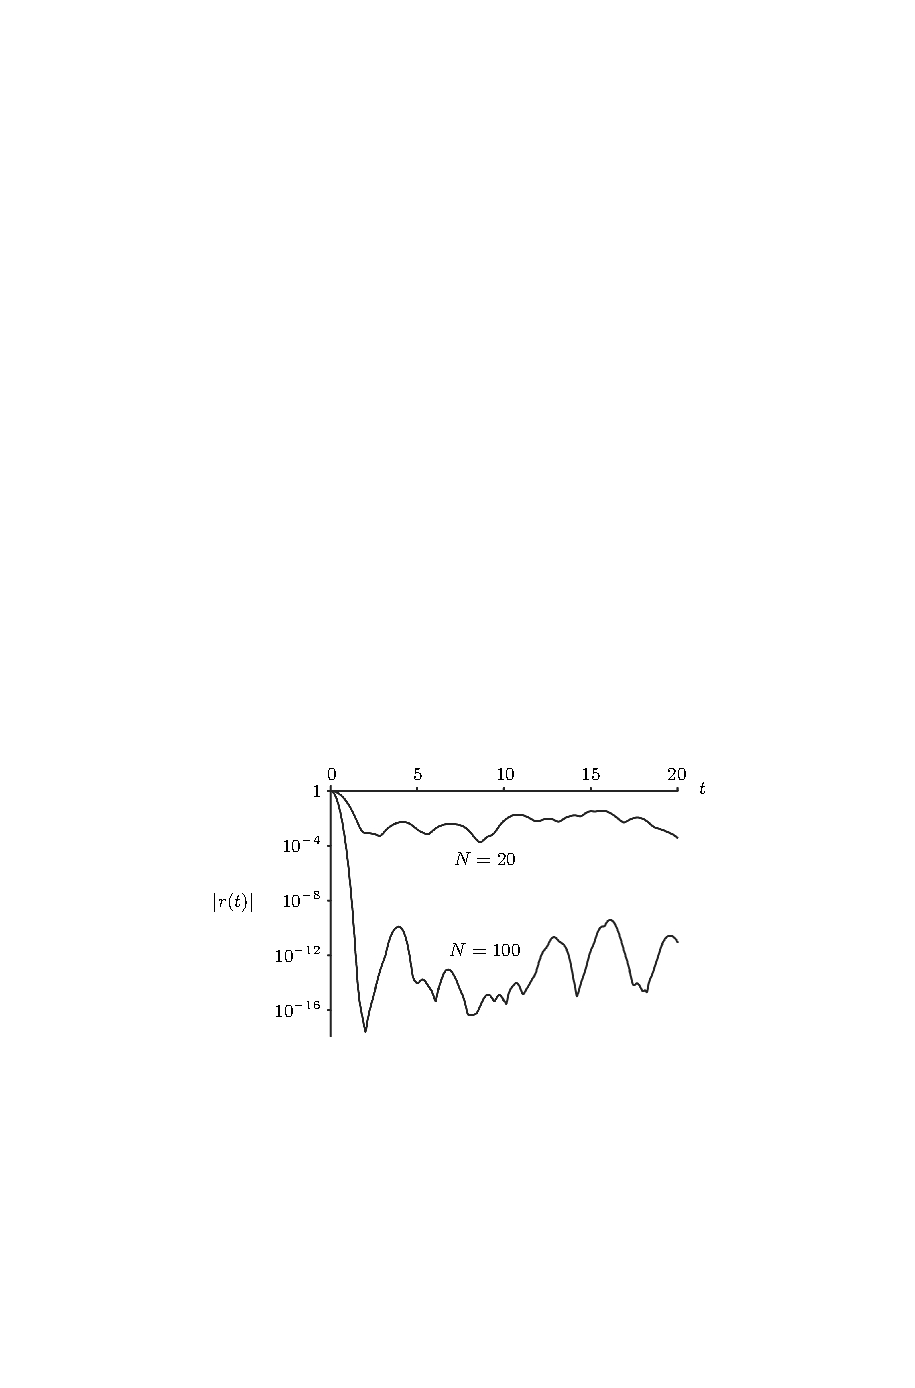
\includegraphics[width=.84\linewidth]{figures/ch02_fig06.pdf}\caption{デコヒーレンス因子$r(t)$［式(2.107)］の絶対値の発展。$N$個の静的な環境スピンの集まりと相互作用する、静的な中心スピン系の干渉項の時間依存性を、異なる二つの値$N=20$、$N=100$について記述する。各環境スピンの初期状態は完全にランダムとし、環境スピンは相互にも、系とも完全に無相関とした。結合は区間$[0,1]$からランダムに選んだ。}\end{figure}

しかし環境スピン数、したがって環境自由度数が有限である限り、デコヒーレンス因子(2.107)が初期値の1へ戻る、特徴的な回帰時間$\tau_{\mathrm{rec}}$が必ず存在することを認識するのが重要である。これは単に、式(2.107)が時間的に周期的な関数の和であることの帰結である。そのような周期関数の和は、それ自体も周期的でなければならない。回帰時間の値は、環境の初期状態と結合$g_i$の分布による。たとえば、環境スピン間に初期相関がない、高度に「非ランダム」な環境の初期状態
\begin{equation}\lvert\Psi(0)\rangle=(a\lvert0\rangle+b\lvert1\rangle)\prod_{i=1}^N\frac1{\sqrt2}(\lvert\uparrow\rangle_i+\lvert\downarrow\rangle_i)\tag{2.111}\end{equation}
という極限で、すべての$i$について$g_i=g$とすると、式(2.107)は

% 原文 p.93
\hypertarget{srcpage:93}{}\label{srcpage:93}
\begin{equation}r(t)=\cos^N(gt)\tag{2.112}\end{equation}
を与える。このデコヒーレンス因子は振動数$g/2\pi$で周期的である。したがって、その絶対値$\lvert r(t)\rvert$が減衰を示すのは$t<\pi/g$の時間だけで、$\tau_{\mathrm{rec}}=\pi/g$の整数倍の時刻に、コヒーレンスの完全な復活が起こる。また環境が、たまたま$\hat E$の固有状態$\lvert n\rangle$の一つから出発する極端な状況では、$r(t)$はまったく減衰せず、したがってデコヒーレンスも起こらない。

現実的な場合、このように高度に秩序立った初期状態と、対称的な系と環境の結合が、関係する可能性は低い。その場合、特徴的な回帰時間$\tau_{\mathrm{rec}}$は通常、きわめて長く、$\tau_{\mathrm{rec}}\propto N!$というPoincaré型になる。現実的だが有限の大きさの巨視的環境では、Zurek\cite{ref009}が最初に指摘したように、$\tau_{\mathrm{rec}}$は宇宙の寿命を超えうる。したがって系からのコヒーレンス喪失が、通常、実際上あらゆる目的に対して不可逆なのは、環境を制御し観測する実際上の能力がないだけでなく、ほぼすべての物理的に現実的な状況で、コヒーレンス回帰の時間尺度が天文学的に大きいからでもある。

% 原文 p.93（後半）


\subsectionlink{デコヒーレンスと散逸}
系からのエネルギーの喪失である散逸は、古典的な効果である。系を、環境と呼んでもよい他の系と相互作用させると、両者の間ではしばしばエネルギー交換が起こり、最終的に系は熱平衡に近づく。これが起こる特徴的時間尺度は、通常、その系の緩和時間尺度と呼ばれる。特定の系と環境の相互作用が、系に散逸をもたらす場合、その相互作用の強さは、緩和時間の尺度となる。相互作用が弱くなるほど緩和時間は長くなり、逆も成り立つ。

しかし、散逸がないか無視できるとしても、系と環境の相互作用がない、または無視できると結論してはならない。ある型の相互作用が散逸をもたらさなくても、一般には、純粋な量子効果であるデコヒーレンスを起こす。すなわち環境は一般に、系のエネルギーをまったく吸収せずに、経路情報、または、より一般的にどの状態かという情報を得られる。前の2.10節の模型は、そのような散逸を伴わないデコヒーレンスの、最初の具体例を与えた。したがって、デコヒーレンスは散逸を伴ってもよいが、伴う必要はない。一方、散逸が存在するなら、デコヒーレンスも起こる。

散逸とデコヒーレンスの両方がある場合には、両者の時間尺度は大きく異なるため、通常はかなり容易に区別できる。

% 原文 p.94
\hypertarget{srcpage:94}{}\label{srcpage:94}
多数の理論的・実験的研究が示したように、デコヒーレンス時間は通常、緩和時間より何桁も短い。5.2.4節では、距離$\Delta x$だけ離れた、二つの異なる位置の重ね合わせで記述される、質量を持つ物体について、緩和時間$\tau_r$とデコヒーレンス時間$\tau_d$の比の、おおよその評価が
\begin{equation}\frac{\tau_r}{\tau_d}\sim\left(\frac{\Delta x}{\lambda_{\mathrm{dB}}}\right)^2\tag{2.113}\end{equation}
であることを示す。ここで$\lambda_{\mathrm{dB}}$は、物体の熱的de Broglie波長、
\begin{equation}\lambda_{\mathrm{dB}}=\frac{\hbar}{\sqrt{2mk_{\mathrm B}T}}\tag{2.114}\end{equation}
であり、$m$は物体の質量、$T$は温度、$k_{\mathrm B}$はBoltzmann定数である。式(2.113)は、Zurekが1984年に導出し\cite{ref012}、当時はまだ「脱相関時間」と呼んだデコヒーレンス時間の、最初の一般的評価を与えた。

Zurekはその論文と、その後のPhysics Todayの記事\cite{ref013}で、巨視的水準でのデコヒーレンスと緩和の時間尺度が、通常いかに大きく違うかを示すため、次の数値例を与えた。室温$T=300\,\mathrm K$で、質量$m=1\,\mathrm g$の巨視的物体を考えた。この物体の$\lambda_{\mathrm{dB}}$は微小で、約$10^{-23}\,\mathrm m$である。明らかにこれは、どの意味でも微視的な数である。いま粒子が、中間的、さらには巨視的に区別可能な二位置の、コヒーレントな重ね合わせで記述されるとしよう。すると式(2.113)の比$(\Delta x/\lambda_{\mathrm{dB}})^2$は非常に大きく、この重ね合わせのデコヒーレンス時間$\tau_d$は、散逸、すなわち緩和時間$\tau_r$より圧倒的に短いことが従う。Zurek\cite{ref012,ref013}は、物体が、巨視的な距離$\Delta x=1\,\mathrm{cm}$だけ離れた二つの空間位置の重ね合わせで記述される例を用いた。この場合、比(2.113)は$10^{40}$程度となる。すなわち、その重ね合わせで記述される物体の典型的デコヒーレンス時間は、熱平衡に達する緩和時間より、約40桁も短いのである。

したがって巨視的物体では、環境によるデコヒーレンスに関係する、どの時間尺度での系の力学についても、環境の散逸的影響は、通常まったく無視できる。たとえばボウリングの球に散乱される光子は、球の運動にはほとんど影響しない一方、球の巨視的に識別できる位置を含む重ね合わせ状態には、ほぼ瞬間的なデコヒーレンスをもたらす（図1.3も参照）。

このように、緩和時間とデコヒーレンス時間の決定的な違いは、なぜ巨視的物体が、デコヒーレンスの作用によって実効的に「作り出される」（5.2.5節）、完全にNewton的な軌道を進むと観測されながら、物体の減速など、散逸の現れがほとんどない場合が多いのかを説明する。Joosに由来する例\cite[p.~79]{ref017}を用いれば、木星は何十億年も太陽の周りをNewton的軌道で公転している一方、その運動状態は、表面で散乱される太陽光による散逸的損失、すなわち摩擦に、ほとんど影響されていない。緩和時間とデコヒーレンス時間が実際に同程度なら、明らかに、この事実を説明するのは非常に難しいだろう。

% 原文 p.95
\hypertarget{srcpage:95}{}\label{srcpage:95}
\subsectionlink{デコヒーレンスと古典的雑音}
本書では、一貫して「デコヒーレンス」という語を、何らかの環境との、通常は実際上不可逆な量子もつれの帰結を記述するために限って使う。これは、歴史的に確立した意味、および環境デコヒーレンスの膨大な文献と一致する。2.6節、2.7節で詳しく述べたように、デコヒーレンスの基本機構は、次のように形式化できる。系$\mathcal S$に、環境$\mathcal E$との相互作用の過程で、もつれが最小になるという性質によって定義される、指針状態の組$\{\lvert s_n\rangle\}$があるとする。
\begin{equation}\lvert s_n\rangle\lvert E_0\rangle\longrightarrow\lvert s_n\rangle\lvert E_n\rangle.\tag{2.115}\end{equation}
すると、指針状態$\lvert s_n\rangle$の任意の純粋状態の重ね合わせ$\sum_n c_n\lvert s_n\rangle$は、なじみ深いもつれ状態
\begin{equation}\left(\sum_n c_n\lvert s_n\rangle\right)\lvert E_0\rangle\longrightarrow\sum_n c_n\lvert s_n\rangle\lvert E_n\rangle\tag{2.116}\end{equation}
をもたらす。2.7節で述べたとおり、縮約密度行列の形式では、これは$\{\lvert s_n\rangle\}$基底の非対角項の減衰をもたらす。
\begin{equation}\hat\rho_{\mathcal S}=\sum_{nn'}c_nc_{n'}^*\lvert s_n\rangle\langle s_{n'}\rvert\langle E_{n'}\vert E_n\rangle\longrightarrow\sum_n\lvert c_n\rvert^2\lvert s_n\rangle\langle s_n\rvert.\tag{2.117}\end{equation}
環境の相対状態$\lvert E_n\rangle$が、急速に相互直交、すなわち識別可能になるからである。明らかに、相互作用(2.116)は、$\mathcal S$のどの成分状態にも力学的変化を生まず、唯一の効果は純粋で非局所的な量子もつれである。したがって、デコヒーレンスは、古典的類似物を持たない、明確に量子力学的な効果として理解すべきである。これが、本書で用いるデコヒーレンスの形式と物理的解釈である。

しかし読者は文献で、他のいくつかの過程が、ときに「デコヒーレンス」と呼ばれたり、形式的、物理的などの意味で、それと「同値」と主張されたりする説明に出会うかもしれない。このような結び付けの大半は、異なる過程がいずれも、系の密度行列の、ある基底における非対角要素の消失に至りうる、という観察に基づく。しかし密度行列による記述は、形式的道具にすぎず、密度行列の形式では効果が似た表現を持つ過程の、決定的な物理的・概念的相違を、やや誤解させやすく、欺くように隠すことを、強調するのが重要である。

% 原文 p.96
\hypertarget{srcpage:96}{}\label{srcpage:96}
たとえば量子工学者や実験家として実際的な立場を採ると、純粋な環境とのもつれとは異なる過程に「デコヒーレンス」という語を結び付けることが、時には実際に正当化される場合もあるが、それらの根本的解釈は、本書の意味での「真の」デコヒーレンスとは異なる。これは単なる哲学的問題ではない。形式的に似た密度行列記述の基礎にある、異なる物理過程を、少なくとも原理上区別できる実験手順が、常に存在する。

Joos\cite{ref017}の作った語を用いた「偽のデコヒーレンス」の、最も一般的で重要な例は、雑音を含む系の異なる実現についての集団平均の結果を、デコヒーレンス過程の記述と解釈することである。これは、密度行列の形式に現れる形式的類似によって、物理的デコヒーレンス過程へ誤って分類する例をなす。この混同の起源は、物理的に非常に異なる二つの設定を記述するために、密度行列を使うことに遡れる。一方で、密度行列の形式は、真の物理的集団、すなわち、各系が純粋状態で記述される$N$個の物理系の集まりを記述するために、しばしば用いられる（2.4.5節の議論も参照）。たとえば各系が、基底状態$\lvert0\rangle$、$\lvert1\rangle$に張られる2次元Hilbert空間で表され、第$i$系の純粋状態が
\begin{equation}\lvert\psi_i\rangle=\frac1{\sqrt2}(\lvert0\rangle+\lvert1\rangle e^{i\phi_i})\tag{2.118}\end{equation}
で与えられるとする。ここで$e^{i\phi_i}$は、各系に固有の相対位相因子である。この位相因子の生じ方は二通りある。第一に、各系が初めから、わずかに異なる初期状態に準備されているかもしれない。あるいは、すべての系が同じ状態から出発しても、わずかに異なるHamiltonianに従うかもしれない。たとえば、各系のHamiltonian$\hat H_i$のポテンシャルが、ランダムな揺らぎ$V_i(t)=V_0(t)+\delta V_i(t)$を含みうる\cite{ref121}。いずれの場合も、異なる系の相対位相因子の違いは、系の準備中、またはその後の発展中に加わる古典的雑音の存在によると考えられる。

$N$個すべての系の純粋状態の集団$\{\lvert\psi_i\rangle\}$について平均すると、集団の密度行列

% 原文 p.97
\hypertarget{srcpage:97}{}\label{srcpage:97}
\begin{equation}\begin{split}\hat\rho&=\frac1N\sum_{i=1}^N\lvert\psi_i\rangle\langle\psi_i\rvert\\&=\frac12\lvert0\rangle\langle0\rvert+\frac12\lvert1\rangle\langle1\rvert\\&\quad+\left(\frac1{2N}\sum_{i=1}^Ne^{i\phi_i}\right)\lvert1\rangle\langle0\rvert+\left(\frac1{2N}\sum_{i=1}^Ne^{-i\phi_i}\right)\lvert0\rangle\langle1\rvert\end{split}\tag{2.119}\end{equation}
を得る。$N$が大きい極限では、ランダムな位相因子$e^{\pm i\phi_i}$の和が、平均して零になるため、
\begin{equation}\hat\rho\longrightarrow\frac12\lvert0\rangle\langle0\rvert+\frac12\lvert1\rangle\langle1\rvert.\tag{2.120}\end{equation}
明らかに、この「集団の位相緩和」は、$\{\lvert0\rangle,\lvert1\rangle\}$基底でデコヒーレンスを起こす個々の系の縮約密度行列と、同じ対角形の密度行列を生む。しかし式(2.119)、(2.120)で干渉項$\lvert0\rangle\langle1\rvert$、$\lvert1\rangle\langle0\rvert$が消えるのは、系の物理的集団の多数の要素について、言い換えれば、特定の雑音過程の異なる実現について、数学的平均を取った結果にすぎない。それは、個々の系の位相コヒーレンスの非局在化を記述する、私たちの意味でのデコヒーレンスには対応しない。今度は密度行列の形式で力学的位相を平均して生じる、「偽のデコヒーレンス」の別の例が、文献\cite{ref122}で批判的に分析されている。

実際、2.4.5節で指摘したように、各々が式(2.118)の純粋状態$\lvert\psi_i\rangle$で記述される、$N$個の物理系の集団の正しい記述は、すべての状態$\lvert\psi_i\rangle$の、純粋状態のテンソル積
\begin{equation}\lvert\Psi\rangle=\prod_{i=1}^N\lvert\psi_i\rangle\tag{2.121}\end{equation}
で与えられる。この状態は$2^N$次元Hilbert空間に「住む」ので、対応する密度行列の大きさは、式(2.119)のような$2\times2$ではなく、$2^N\times2^N$である。環境との相互作用なしでは、各系は完全にユニタリに発展し、したがって位相関係$\phi_i$は、常に明確に保たれる。式(2.119)のように、多くの物理系の集団平均を表すために密度行列の形式を使うと、形式的にだけ位相が「洗い流された」ように見えるが、位相は系から物理的に非局在化してはいないので、少なくとも原理上、各系の観測者には実験的にアクセスできるままである。雑音過程の時間発展を知っていれば、適切なユニタリな逆変換を系に加えて、実験の各実行で、雑音の影響を常に完全に逆転できる。この集団の位相緩和の逆転は、たとえばNMR実験で実際に実装されている。そこでは、雑音により各スピンがわずかに異なる振動数で歳差運動するため、スピンの集まりは、やがて位相が揃わなくなる。しかし、適切に選んだ制御パルスを加えると、スピン集団を「再集束」できる。これはスピンエコー法と呼ばれる。

% 原文 p.98
\hypertarget{srcpage:98}{}\label{srcpage:98}
系のHamiltonianへのランダムな揺らぎの追加である雑音は、系と環境の量子もつれを何も作らず、少なくとも原理上、局所操作によって完全に取り消せる。これに対しデコヒーレンスは、系が環境自由度ともつれ、位相関係が実際上すべての目的に対して不可逆に系から失われ、系への局所測定では、もはやアクセスできなくなることを意味する。それに対応して、系の情報が環境に刻まれる。したがって古典的雑音の場合には、系が環境に乱されるが、式(2.115)は、デコヒーレンスが、系が環境を乱す状況を記述することを示す（文献\cite{ref016}のIV.C節も参照）。すると量子状態の非局所的性格によって、系が環境に与えたこの「歪み」が、今度は系の水準で観測できるものに影響する。これは形式的には縮約密度行列で記述される。しかし2.11節で論じたように、この影響は、環境が与える古典的雑音による系の擾乱よりも、通常ははるかに短い時間尺度で起こる。

確率的揺らぎ、すなわち古典的雑音過程は、環境の系への影響を模擬するためにも、しばしば使われる。その場合、系に加える確率的な「蹴り」によって、デコヒーレンスを模型化する（たとえば文献\cite{ref121,ref123,ref124,ref125}）。もちろん、上で論じたのと同じ問題がここにも当てはまる。古典的雑音を系に加えることは、ランダムに揺らぐHamiltonianで支配される、閉じた系のユニタリ発展に対応する。一方デコヒーレンスは、開いた量子系が、他の量子系、すなわち環境と、決定論的にもつれることで表される。一般に、これら二つの状況から生じる系の量子状態は、異なる観測可能な性質を持つ\cite{ref121}。ある場合にだけ、古典的雑音によるデコヒーレンスの模擬は、密度行列の記述の水準で、形式的に似た結果を与える。しかし、そのような場合でも、雑音とデコヒーレンスの根本的で概念的な相違は残る。7.3節では、量子計算の文脈で、特に、雑音によってデコヒーレンスを実験的・理論的に模擬することに関し、これらの違いをさらに論じる。

% 原文 p.98（後半）


\subsectionlink{仮想デコヒーレンスと量子的「消去」}
2.7節で論じたように、系と相互作用する多数の自由度を制御できないことによって生じる、局所的な位相関係の非局在化の実効的不可逆性は、デコヒーレンスの目印である。そのような「実の」デコヒーレンスと、真に、あるいは実効的に可逆な位相の非局在化を区別し、後者を仮想デコヒーレンスと呼ぶ。

% 原文 p.99
\hypertarget{srcpage:99}{}\label{srcpage:99}
位相の非局在化を真に逆転し、重ね合わせを系の水準に再局在化できる可能性は、大域的な系と環境の発展が完全にユニタリであることに基づく。系と環境の組合せに適切なユニタリ逆変換を加えれば、系と環境のもつれがほどけ、元の分離可能な系と環境の積状態を力学的に回復する。このデコヒーレンスの完全な逆転は、実質的に時間の矢の逆転に対応し、波動関数の成分を局所的に再結合する、実際の再コヒーレンス過程を記述する。これは、磁場によって分離された二本の原子ビームを、その後再結合、つまり再集束する、可逆なStern--Gerlach実験\cite{ref126,ref127}に類似する。実際には、そのような可逆なデコヒーレンスは、「人工的環境」として働く、完全に制御された第二の系へ、系を結合することによって、実験的に研究できるだろう。この考えを実験で実現するための具体的提案を、6.1.4節で論じる。

系に対するデコヒーレンスの影響は、デコヒーレンス前の元の重ね合わせ状態を再構成することによっても、実効的に逆転できる。そのような元の状態の実効的再構成の例は、量子消去という名で知られるようになった\cite{ref075,ref128,ref129,ref130}。同様の考えは、量子コンピュータの誤り訂正の概念の基礎にもある（7.4節）。量子的「消去」の基本方式は、文献では典型的に次のように述べられる（たとえば文献\cite{ref130}）。引用符を付ける理由は後に説明する。再び二重スリット実験を考え、経路検出器が、粒子がどのスリットを通るかを測定する。系と検出器の複合発展は、式(2.65)、すなわち
\begin{equation}\frac1{\sqrt2}(\lvert\psi_1\rangle+\lvert\psi_2\rangle)\lvert\text{「準備完了」}\rangle\longrightarrow\frac1{\sqrt2}(\lvert\psi_1\rangle\lvert1\rangle+\lvert\psi_2\rangle\lvert2\rangle)\tag{2.122}\end{equation}
の形となる。経路検出器に、明示的な読み出し装置を結合する。測定相互作用は
\begin{equation}\lvert\pm\rangle\lvert\Phi_0\rangle\longrightarrow\lvert\pm\rangle\lvert\Phi_\pm\rangle\tag{2.123}\end{equation}
と仮定する。ここで$\lvert\Phi_0\rangle$は読み出し装置の初期状態、$\lvert\pm\rangle$は経路検出器の共役状態、
\begin{equation}\lvert\pm\rangle\equiv\frac1{\sqrt2}(\lvert1\rangle\pm\lvert2\rangle)\tag{2.124}\end{equation}
である。その結果、粒子、経路検出器、読み出し装置からなる全系の発展は、次となる。

% 原文 p.100
\hypertarget{srcpage:100}{}\label{srcpage:100}
\begin{equation}\begin{split}
&\frac1{\sqrt2}(\lvert\psi_1\rangle+\lvert\psi_2\rangle)\lvert\text{「準備完了」}\rangle\lvert\Phi_0\rangle\\
&\quad\longrightarrow\frac1{\sqrt2}(\lvert\psi_1\rangle\lvert1\rangle+\lvert\psi_2\rangle\lvert2\rangle)\lvert\Phi_0\rangle\\
&\quad=\frac1{\sqrt2}(\lvert\psi_+\rangle\lvert+\rangle+\lvert\psi_-\rangle\lvert-\rangle)\lvert\Phi_0\rangle\\
&\quad\longrightarrow\frac1{\sqrt2}(\lvert\psi_+\rangle\lvert+\rangle\lvert\Phi_+\rangle+\lvert\psi_-\rangle\lvert-\rangle\lvert\Phi_-\rangle).
\end{split}\tag{2.125}\end{equation}
ここで$\lvert\psi_\pm\rangle$は式(2.79)で定義した共役状態である。

発展(2.125)は、読み出し装置が、粒子の経路の情報を含まない経路検出器の状態、すなわち$\lvert\pm\rangle$と量子的に相関することを示す\footnote{状態$\lvert+\rangle$、$\lvert-\rangle$の一方で記述される検出器について、二つの可能な経路のどちらを記録したかを調べる測定をすると、結果$\lvert1\rangle$、$\lvert2\rangle$は等しい確率で得られるからである。}。量子力学の標準的な収縮の描像では、読み出し装置の測定は、式(2.125)の右辺の終状態を、成分$\lvert\psi_+\rangle\lvert+\rangle\lvert\Phi_+\rangle$と$\lvert\psi_-\rangle\lvert-\rangle\lvert\Phi_-\rangle$の一方へ射影する。言い換えれば測定は、粒子の経路を推論できない状態に、系を「強制」する。

したがって、経路成分$\lvert\psi_1\rangle$、$\lvert\psi_2\rangle$の間の干渉は、重ね合わせ$\lvert\psi_\pm\rangle$に具現されるように、実際の局所的な再コヒーレンス過程とは違い、非局所的に回復される。この意味で、系の初めの重ね合わせ$\lvert\psi_+\rangle$、または位相を逆にした$\lvert\psi_-\rangle$が再構成される。そのため消去は、粒子がスクリーンに記録された後まで遅らせてもよい。そのような「遅延選択」実験（たとえば文献\cite{ref131}）の精神は、Wheelerが初めて提案した思考実験\cite{ref041}に遡る。量子的「消去」は、光子による二重スリット実験\cite{ref135}を含む、いくつかの実験\cite{ref131,ref132,ref133,ref134,ref135}で実証された。

しかし「量子消去」という用語は、かなり誤解を招くことを強調しておく。これを見るため、二つの場合を区別しよう。第一に、粒子と経路検出器の相互作用(2.122)が、不可逆だと仮定してよい。これは真の意味の測定を記述する。不可逆性を測定の定義的性質と見なせることを思い出そう。開いた系の描像では、この不可逆性は、不可避な環境相互作用と、その結果として成分状態$\lvert\psi_1\rangle\lvert1\rangle$、$\lvert\psi_2\rangle\lvert2\rangle$間の位相関係が非局在化することから生じる。そのとき経路測定の記録は、アクセス不能な環境に消えないよう刻まれるので、実際にこの情報を消去できない\footnote{もちろん、この議論では、経路測定の不可逆性の具体的な起源は重要でない。たとえば、単に波動関数の収縮が不可逆性をもたらすと仮定してもよい。}。

% 原文 p.101
\hypertarget{srcpage:101}{}\label{srcpage:101}
あるいは、式(2.122)を、可逆で、したがって仮想的でしかない、経路「測定」を記述すると見なしてもよい\footnote{ここで引用符を使うのは、可逆な相互作用を正当な測定と見なすのが難しいことを、明確にするためである。また式(2.125)の第一行から第二行へ、粒子と検出器のもつれ状態を変換すると、経路検出器がそもそも何を「測定」したのかという問いが、未解決のままになることにも注意しよう。式(2.125)の第一行からは、系の$\{\lvert\psi_1\rangle,\lvert\psi_2\rangle\}$基底の「測定」を推論するが、第二行は、共役基底$\{\lvert\psi_+\rangle,\lvert\psi_-\rangle\}$の「測定」を意味する。もちろん、これは単に2.5.2節の優先基底の問題である。}。古典物理学では、「消去」は、たとえば熱への変換による、情報の不可逆な破壊に対応する\cite{ref136}。量子的状況の類似の過程は、可逆な経路「測定」の仮想的な「結果」$\lvert1\rangle$、$\lvert2\rangle$を、以前に記録した粒子の経路に、制御されない仕方で依存し、そのためもはや経路情報を符号化しない、新たな状態$\lvert d_1\rangle$、$\lvert d_2\rangle$へ、不可逆に変えることで表される。したがって経路情報の観点では、$\lvert d_1\rangle$、$\lvert d_2\rangle$は区別できず、まとめて$\lvert d_0\rangle$と書いてよい。このリセット\cite{ref136,ref137}は、たとえば熱浴として実現される、制御されない情報の「排出先」に検出器を結合して、次の形の実効的に不可逆な発展を起こすことで達成できる。
\begin{equation}\begin{split}
&\frac1{\sqrt2}(\lvert\psi_1\rangle\lvert1\rangle+\lvert\psi_2\rangle\lvert2\rangle)\lvert\chi_0\rangle\\
&\quad\longrightarrow\frac1{\sqrt2}(\lvert\psi_1\rangle\lvert d_1\rangle\lvert\chi_1\rangle+\lvert\psi_2\rangle\lvert d_2\rangle\lvert\chi_2\rangle)\\
&\quad\equiv\frac1{\sqrt2}(\lvert\psi_1\rangle\lvert\chi_1\rangle+\lvert\psi_2\rangle\lvert\chi_2\rangle)\lvert d_0\rangle.
\end{split}\tag{2.126}\end{equation}
ここで$\lvert\chi_0\rangle$は排出先の初期状態である。元の経路検出器の状態$\lvert1\rangle$、$\lvert2\rangle$の差は、決定論的に排出先へ転送されなければならず、それによって検出器のエントロピーが増え、初めの可逆な経路「測定」から得た情報を補償する。したがって排出先の状態$\lvert\chi_1\rangle$、$\lvert\chi_2\rangle$は識別可能であり、式(2.126)で実装する真の経路情報の消去は、明らかに粒子に追加の空間的デコヒーレンスを導入し、今度は必然的に不可逆となる。消去過程(2.126)は、発展(2.125)と大きく異なる。実際、式(2.125)が成り立つためには、式(2.126)の意味で経路情報の不可逆な破壊、すなわち実際の消去は、起こってはならない。

% 原文 p.101（後半）


\subsectionlink{部分系への分解}
デコヒーレンスは、世界を「系」と「環境」に分けることの存在と可能性を、前提とすることに注意しよう。デコヒーレンス研究計画では、「環境」という語は、通常、系の「残り」として理解される。すなわち環境自由度は、典型的には制御しない、制御できない、または制御する必要がなく、考えている観測に直接関係しないが、それでも環境は、系の状態の発展に有意に寄与するすべての自由度を含む、という意味である。これは本質的に、Zurekのデコヒーレンスと指針状態に関する最初の論文\cite[p.~1520]{ref008}で与えられた定義である。

% 原文 p.102
\hypertarget{srcpage:102}{}\label{srcpage:102}
この系と環境の二元性は、一般に量子もつれと関係する。量子もつれは常に、宇宙の部分間の相関を記述する。宇宙を個々の部分系へ分解しない限り、測定問題はない。宇宙全体の状態ベクトル$\lvert\Psi\rangle$\footnote{この全状態を、あえて仮定するならば、である。Aulettaの反論\cite{ref138}を参照。}はSchrödinger方程式に従って決定論的に発展し、そこに解釈的な困難はない。測定問題は、宇宙の全Hilbert空間$\mathcal H$を、二空間の積$\mathcal H_1\otimes\mathcal H_2$へ分解し、一方の部分系に個別の状態を割り当てようとしたときにだけ生じる。Zurek\cite[p.~718]{ref016}は、こう表現する。
\begin{quote}
系が存在しなければ、解釈の問題は消えるように見える。系のない宇宙には、単に「収縮」が必要ない。古典的実在についての私たちの経験は、外から見た宇宙全体ではなく、その内部の系に当てはまるのである。
\end{quote}
さらに、「観測」「相関」「相互作用」といった語も、系への分割なしには、当然ほとんど意味を持たない。Zehは、いかなる観測も宇宙の一部についての無知から生じるという意味で、観測者の局所性が観測を定義し、この局所性が、量子系に起こりうる「事実」も定義すると示唆した。Landsman\cite[pp.~45--46]{ref139}も同様に論じる。
\begin{quote}
量子力学における「測定」「事実」「出来事」の本質は、当該の系のある部分を観測しないこと、あるいはその部分が無関係であることにある。（中略）無関係と宣言された、または無関係であることを強いられる部分のない世界は、事実のない世界である。
\end{quote}
しかし、測定問題の出現とデコヒーレンス研究計画の定式化に、どれほど必要に見えるとしても、宇宙を部分系へ分解するという仮定は、決して自明ではない。定義により宇宙全体は閉じた系なので、外部環境の「観測されない自由度」はない。したがって、「大域的」な準古典的観測可能量を決めるために、デコヒーレンス理論を宇宙全体へ適用することはできない。また全Hilbert空間を、どのように部分系へ分けるかについての一般的基準はない一方、系の性質と呼ばれるものの多くは、他の系との相関に依存する。この問題は、デコヒーレンスに、古典性の主観的知覚の説明を動機付けるだけでなく（たとえば8.2節、9.4節）、準古典的な「巨視的事実」の定義まで可能にさせたい場合に、とりわけ深刻になる。

% 原文 p.103
\hypertarget{srcpage:103}{}\label{srcpage:103}
Zurek\cite[p.~1820]{ref104}は、この概念的な難点を、最初期に明瞭に指摘した一人である。
\begin{quote}
特に、しばしば当然視されてきた一つの問題が、デコヒーレンス研究計画全体の基礎として、大きく立ちはだかっている。それは、古典性の出現についてのあらゆる議論で、それほど決定的な役割を果たす「系」とは何かという問いである。（中略）系とは何か、たとえば適切に大きなHilbert空間内の全体のHamiltonianが与えられたとき、それらをどう定義するかについての説得的説明は、疑いなく、きわめて有用であろう。
\end{quote}
よく提案される考えは、「絶対的」分解という概念を捨て、代わりに、異なる状態空間と、それら相対的に定義された空間間の相関を通じて現れる性質の、本質的な相対性を仮定することである（たとえば、デコヒーレンスとは関係しない提案\cite{ref140,ref141,ref142,ref143}）。系と相関についてのこの相対的な見方は、非古典的という意味で、反直観的な含意を持つ。しかし量子もつれの場合と同じく、これらの含意を、さらなる解決を要するパラドックスと見なす必要はない。自然のある性質を反直観的なものと受け入れることは、本質的に局所的な観測に基づく経験の範囲が許す限り、完全で客観的な自然の記述に至るために、実際に満足できる道である。

\subsectionlink{形式的な道具とその解釈}
ここで、デコヒーレンスの文脈でよく使われ、参照される、いくつかの形式的手順を簡単に概説する。2.15.1節では、二部分系の状態を、von Neumann測定の完了時の終状態を思わせる対角形に常に書けることを教える、Schmidt分解定理を導入する。Schmidt分解とデコヒーレンスの間の、意味のあるつながりと、見せかけのつながりの両方を論じる。2.15.2節では、密度行列のWigner表示を導入する。この表示は、位相空間でデコヒーレンスを可視化するのに、しばしば便利な道具である。続く2.15.3節では、任意に与えられた密度行列を、より大きな系の純粋状態密度行列について、トレースを取ったものと見なせることを示す。最後の2.15.4節では、演算子和形式を導入する。この形式を、より複雑なデコヒーレンス模型に適用するのは、通常実行不可能だが、環境と相互作用する系の縮約力学を記述するための、非常に一般的な枠組みを与える。

% 原文 p.104
\hypertarget{srcpage:104}{}\label{srcpage:104}
\subsubsectionlink{Schmidt分解}
それぞれHilbert空間$\mathcal H_{\mathcal A}$、$\mathcal H_{\mathcal B}$を持つ二つの系$\mathcal A$、$\mathcal B$を考えよう。Schmidt分解定理\cite{ref144}によれば、複合系$\mathcal{AB}$の任意の純粋状態$\lvert\Psi\rangle$は、常に対角形、または「Schmidt」形
\begin{equation}\lvert\Psi\rangle=\sum_i\lambda_i\lvert a_i\rangle\lvert b_i\rangle\tag{2.127}\end{equation}
で書ける。ここでSchmidt状態$\lvert a_i\rangle$、$\lvert b_i\rangle$は、それぞれ$\mathcal H_{\mathcal A}$、$\mathcal H_{\mathcal B}$の正規直交基底、いわゆるSchmidt基底をなし、展開係数$\lambda_i$は、$\sum_i\lvert\lambda_i\rvert^2=1$を満たす複素数である。しかし、位相因子をSchmidt基底状態へ吸収すれば、これらの係数は、$\sum_i p_i=1$を満たす非負の実数$\sqrt{p_i}$に選べる。したがってSchmidt分解は
\begin{equation}\lvert\Psi\rangle=\sum_i\sqrt{p_i}\lvert a_i\rangle\lvert b_i\rangle\tag{2.128}\end{equation}
と書ける。さらに、この分解が一意であるのは、係数$\sqrt{p_i}$がすべて互いに異なる場合、かつその場合に限ることを示せる。

Schmidt分解の一意性には、2.5.2節の優先基底問題の議論ですでに触れた。そこで、von Neumann測定相互作用の結果として現れ、対角的なSchmidt形にある、系と装置の最終的な複合状態の基底の曖昧さが、その状態から測定された観測可能量を一意に推論できないという問題につながることを示した。

Schmidt定理は、$\mathcal A$、$\mathcal B$の縮約密度行列$\hat\rho_{\mathcal A}$、$\hat\rho_{\mathcal B}$にも直接の含意を持つ。式(2.128)を用いれば、$\hat\rho_{\mathcal A}$は、
\begin{equation}\begin{split}\hat\rho_{\mathcal A}&=\operatorname{Tr}_{\mathcal B}\lvert\Psi\rangle\langle\Psi\rvert\\&=\sum_k\langle b_k\rvert\left[\sum_{ij}\sqrt{p_ip_j}\lvert a_i\rangle\langle a_j\rvert\otimes\lvert b_i\rangle\langle b_j\rvert\right]\lvert b_k\rangle\\&=\sum_i p_i\lvert a_i\rangle\langle a_i\rvert\end{split}\tag{2.129}\end{equation}
で与えられ、同様に
\begin{equation}\begin{split}\hat\rho_{\mathcal B}&=\operatorname{Tr}_{\mathcal A}\lvert\Psi\rangle\langle\Psi\rvert\\&=\sum_i p_i\lvert b_i\rangle\langle b_i\rvert\end{split}\tag{2.130}\end{equation}
となる。

% 原文 p.105
\hypertarget{srcpage:105}{}\label{srcpage:105}
したがって$\hat\rho_{\mathcal A}$、$\hat\rho_{\mathcal B}$は、それぞれ基底$\{\lvert a_i\rangle\}$、$\{\lvert b_i\rangle\}$で対角であり、同じスペクトル$\{p_i\}$を持つ。環境と相互作用する系という、デコヒーレンスに関係する場合に適用すれば、Schmidt定理は、関心のある系の縮約密度行列が、厳密に対角になる正規直交基底を、常に見いだせることを意味する。

したがって密度行列のSchmidt分解とは、単に形式的な対角化と、それが常に可能だという事実を指す。この分解は量子物理学の多くの分野で重要な役割を果たすが、デコヒーレンスの記述や量子力学の解釈的問題への関係は、ときに誤って表現されてきた。これは、デコヒーレンスの効果が、環境の選ぶ特定の基底で、縮約密度行列の非対角要素が消えることとして記述されるため、形式的には密度行列の対角化、つまりまさにSchmidt分解の主題に対応するように見えるからかもしれない。

実際、系の密度行列を各瞬間に対角化して得るSchmidt基底は、優先基底を与える能力について、頻繁に研究されてきた（たとえば文献\cite{ref005,ref006,ref145,ref146}）。そのためSchmidt基底状態を「瞬間的な指針状態」と考える人もいた\cite{ref145}。しかしSchmidt分解は、先験的な物理的意味や解釈上の意味を持たない、純粋な数学的手順である。縮約密度行列に適用したSchmidt定理は、そのような行列はすべて、何らかの基底で対角化できると述べるだけである。しかし、この基底が準古典的性質を表すとは限らない（たとえば文献\cite{ref147,ref148}）。これは、系と環境の相互作用の構造が選ぶ指針基底で、環境によって縮約密度行列が近似的に対角化されることと、際立って異なる。指針状態と密度行列を対角化する状態の重要な相違を、初めて明瞭に述べたのはZurek\cite{ref008}であり、2.8.3節の予測可能性のふるいなど、その後の発展の基礎となった。

他の方法では、瞬間的なSchmidt状態を計算せず、代わりに、系と環境の相互作用の構造が選ぶ基底で、縮約密度行列が近似的に対角になるまで、特徴的なデコヒーレンス時間が過ぎるのを待つ。この過程は、たとえば適切なマスター方程式で記述できる（第4章）。その後、このデコヒーレンスした密度行列を対角化してSchmidt状態を計算する。デコヒーレンスは通常、非常によい近似で、指針基底の縮約密度行列を急速に対角化するため、得られるSchmidt状態は、後者が非常に近い縮退にある場合を除き、環境が超選択する状態と、典型的によく似ている。

この近縮退の特別な状況は、容易に示せる\cite{ref146}。2次元Hilbert空間で記述される系を考える。デコヒーレンスの作用の結果、環境が超選択する基底で表した系の縮約密度行列が、次の形になったとする。

% 原文 p.106
\hypertarget{srcpage:106}{}\label{srcpage:106}
\begin{equation}\rho=\begin{pmatrix}1/2+\delta&\omega^*\\\omega&1/2-\delta\end{pmatrix},\qquad\lvert\omega\rvert\ll1,\quad\delta\ll1.\tag{2.131}\end{equation}
ここで$\lvert\omega\rvert\ll1$は強いデコヒーレンス、$\delta\ll1$は近縮退を表す。デコヒーレンスが厳密な対角化$\omega=0$をもたらせば、任意の固定した$\delta$に対して、$\rho$の固有ベクトルは、理想的指針状態に対応する$(0,1)$、$(1,0)$に比例する。しかし$\omega>0$という近似的対角性と、$\delta\longrightarrow0$という縮退の場合、固有ベクトル、したがってSchmidt状態は、$(\pm\lvert\omega\rvert/\omega,1)$に比例するようになる。これは縮退の場合、瞬間的なものではなく、デコヒーレンスした縮約密度行列を対角化しても、そのSchmidt分解が、環境の超選択する状態とは大きく異なる状態を与えうることを意味する。

まとめると、優先される準古典的指針状態を得るための適切な基準は、環境との量子もつれに対する耐性であることを強調するのが重要である。これらの状態は一般に、系の瞬間的な密度行列を単に対角化しても得られない。しかし多くの状況で、デコヒーレンスした縮約密度行列の固有状態は、準古典的で安定な指針状態をよく近似する。特に、後者に十分な非縮退があるときにはそうである。

% 原文 p.106（後半）


\subsubsectionlink{Wigner表示}
Wigner表示、またはWigner関数は、連続自由度で記述される系に対して、密度行列の代わりに、しばしば用いられる。典型的には、この自由度は系の位置$x$であり、ここではその場合に注目する。系の純粋状態または混合状態の、位置空間密度行列$\rho(x,x')\equiv\langle x\rvert\hat\rho\lvert x'\rangle$が与えられたとき、Wigner関数を\cite{ref149,ref150}
\begin{equation}W(x,p)\equiv\frac1{2\pi}\int_{-\infty}^{+\infty}\mathrm dy\,e^{ipy}\rho(x+y/2,x-y/2)\tag{2.132}\end{equation}
と定義する。ここで$p$は粒子の運動量、あるいは一般的に$x$の共役変数である。

Wigner関数は、位相空間の古典的確率分布と、いくらか似ている。たとえば$W(x,p)$は$x$、$p$の実数値関数であり、$x$、$p$の確率分布$P(x)\equiv\rho(x,x)$、$P(p)\equiv\widetilde\rho(p,p)\equiv\langle p\rvert\hat\rho\lvert p\rangle$は、$W(x,p)$の周辺分布として回復できる。
\begin{align}P(x)=\rho(x,x)&=\int\mathrm dp\,W(x,p),\tag{2.133}\\P(p)=\widetilde\rho(p,p)&=\int\mathrm dx\,W(x,p).\tag{2.134}\end{align}
また、$\int\mathrm dx\int\mathrm dp\,W(x,p)=\operatorname{Tr}(\hat\rho)=1$である。

% 原文 p.107
\hypertarget{srcpage:107}{}\label{srcpage:107}
しかし、Wigner関数と位相空間の確率分布を同一視したくなる、この誘惑を行き過ぎさせてはならないことを示す、重要な注意点がある。最も重要なのは、Wigner関数が一般に、ある領域で負の値を取り、真の確率分布を表せないことを示す点である。実際、純粋状態のWigner関数に負の値がないのは、状態がGaussianである場合、かつその場合に限ると示せる\cite{ref151}。もちろん、この知見は、それほど驚くべきでない。結局、量子力学の不確定性関係は、位置と運動量を任意の精度で同時に決定することを禁じる。したがって、端的に言えば、実際の量子的位相空間分布は、そもそも存在できないのである。

このような注意にもかかわらず、多くの場合、Wigner関数は、位相空間の位置と運動量の相関や、量子的干渉を、うまく可視化してくれる。Wigner関数を使って「二重スリット型」の重ね合わせを表し、位相空間のデコヒーレンスの力学を研究することは、Zurek\cite{ref013}に遡る。本書では、5.2節の量子Brown運動の研究に、Wigner関数を用いる。

Wigner関数の姿について感覚を得るため、位置空間で距離$\Delta x$だけ離れた、二つのGaussian波束の重ね合わせを考えよう（図2.7）。対応するWigner関数を図2.8に示す。二つの主ピークと、振動する模様が見える。直接ピークともしばしば呼ばれる主ピークは、古典的に予想される位相空間領域、すなわち位置は$\Delta x$だけ離れ、運動量方向の広がりは同じ領域にある。したがって、これらは、重ね合わされた二つのピークが記述する「古典的」位相空間分布に似たものを記述すると見なせる。位置空間のかなり狭い局在の帰結である、運動量方向の大きな広がりが明瞭に見える。不確定性原理によれば、位置と運動量の両方で完全に局在することはできず、位置の局在がよいほど、運動量方向の広がりは大きい。

\begin{figure}[htbp]\centering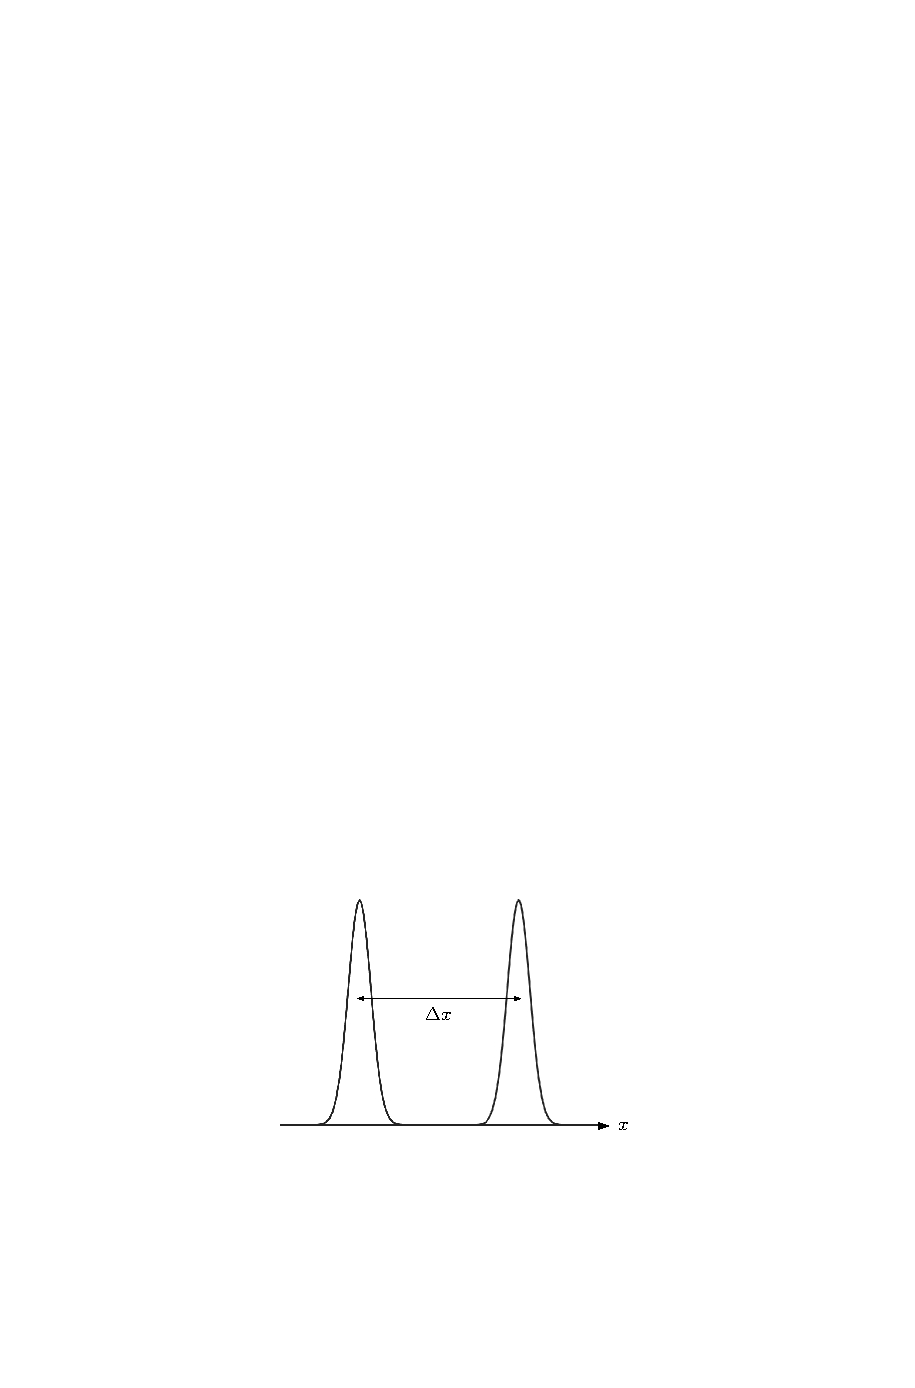
\includegraphics[width=.62\linewidth]{figures/ch02_fig07.pdf}\caption{空間で$\Delta x$だけ離れた、二つのGaussian波束の重ね合わせの図。}\end{figure}

% 原文 p.108
\hypertarget{srcpage:108}{}\label{srcpage:108}
\begin{figure}[htbp]\centering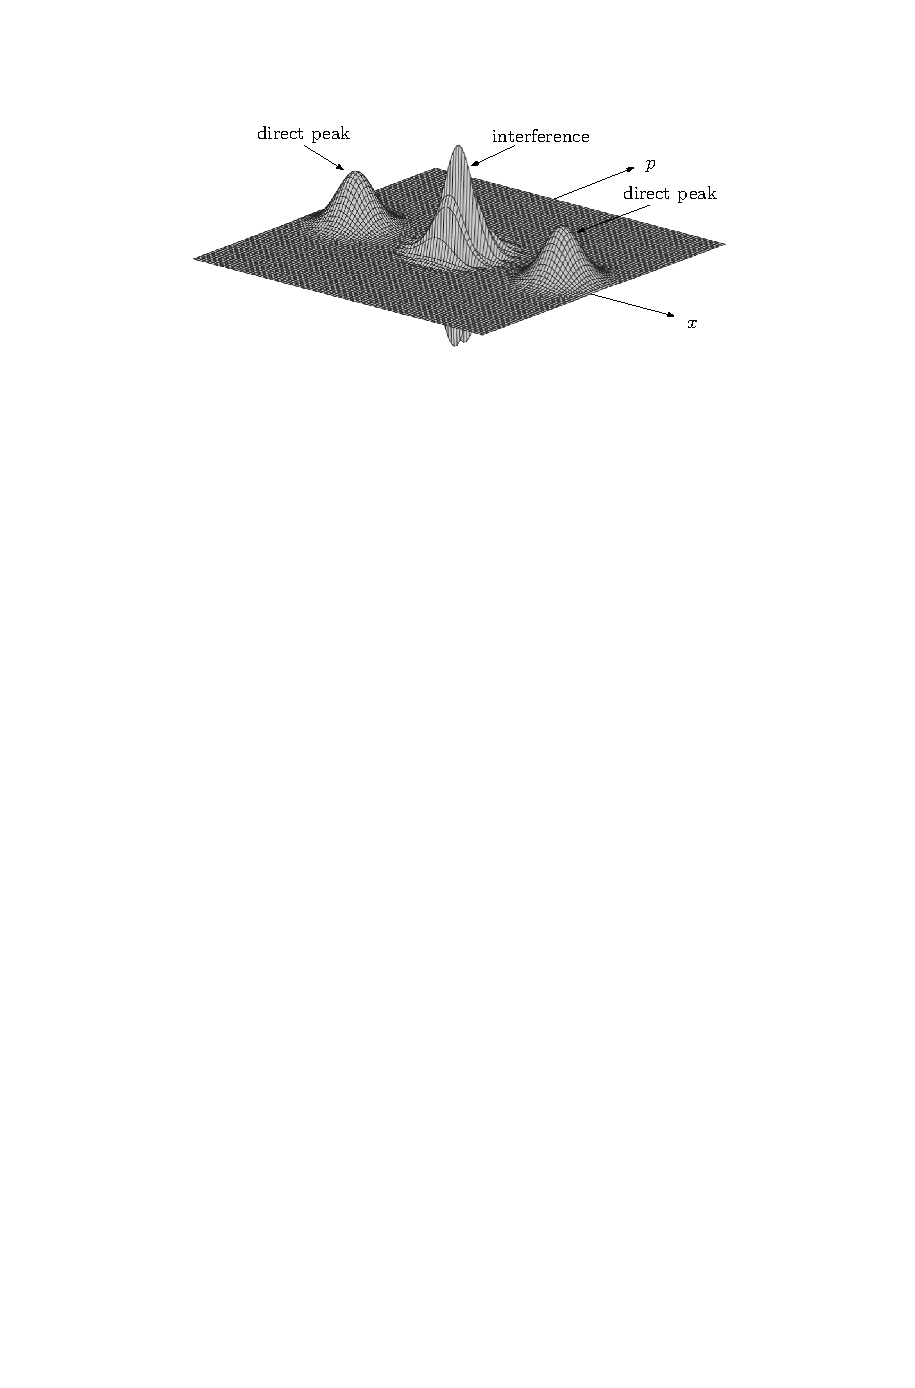
\includegraphics[width=.85\linewidth]{figures/ch02_fig08.pdf}\caption{位置空間で離れた二つのGaussian波束の重ね合わせのWigner表示（図2.7）。}\end{figure}

図2.8に見える、二つの主ピークを結ぶ線に平行な尾根を持つ振動模様は、二波束間の量子干渉が存在する証拠である。系の位置を監視する環境との相互作用が、空間的コヒーレンスを抑制すると、この振動が減衰する（図2.9）。これは、位相空間でデコヒーレンスの作用を可視化する、直観的な方法を与える。

ここで考える、空間的に離れた二つのGaussian波束の重ね合わせでは、Wigner関数の振動模様の振動数$f$が、位置空間の波束間隔$\Delta x$に、
\begin{equation}f=\Delta x/\hbar\tag{2.135}\end{equation}
によって直接関係することを示せる。したがって大まかに言えば、重ね合わせ状態が非古典的になるほど、Wigner関数の振動は速くなる。また図2.8から、特に振動模様の領域で、Wigner関数が負の値を取ることも明瞭に分かる。上で論じたとおり、これは、Wigner関数を古典的な位相空間確率分布と解釈できないことを、直接視覚的に示す。

\begin{figure}[htbp]\centering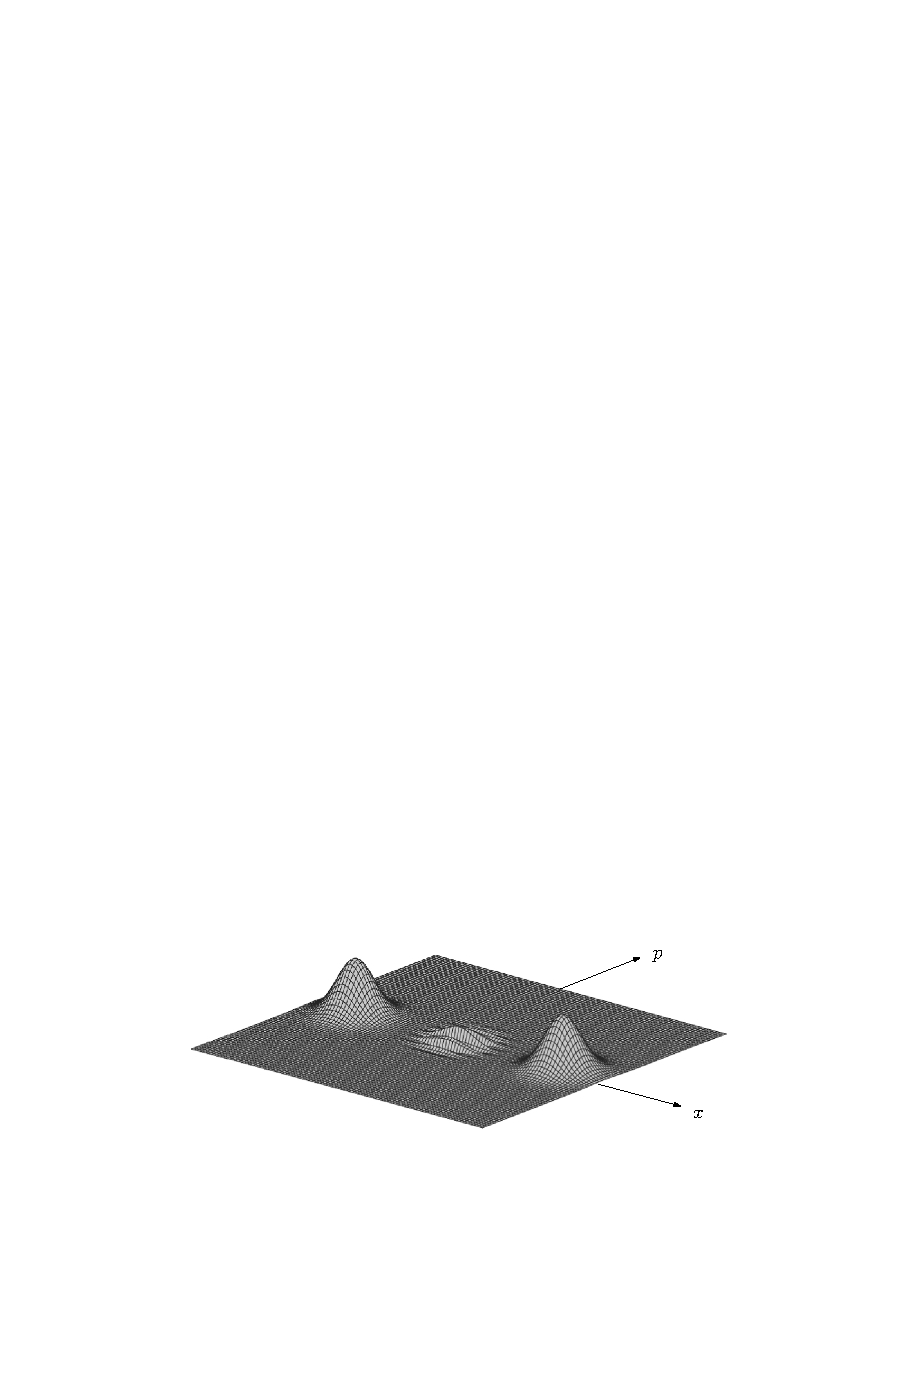
\includegraphics[width=.85\linewidth]{figures/ch02_fig09.pdf}\caption{環境との相互作用と、その結果生じる干渉の抑制は、Wigner表示の振動模様の減衰として現れる（図2.8と比較）。}\end{figure}

% 原文 p.109
\hypertarget{srcpage:109}{}\label{srcpage:109}
\subsubsectionlink{環境の「純粋化」}
2.4.6節でトレース演算を論じた際、より大きな複合系の純粋状態から、部分系の縮約状態を得る方法を示した。私たちの場合、複合系は、関心のある系とその環境である。この手順を「逆にして」、有限次元Hilbert空間で、任意に与えられた非純粋状態を純粋化できることは、驚くべきでない。これは、任意の非純粋状態を、より大きな系の純粋状態の縮約状態と見なせる、という意味である。

証明はまったく直接的である。関心のある系$\mathcal S$が、Hilbert空間$\mathcal H_{\mathcal S}$内の、一般に非純粋な、何らかの密度行列$\hat\rho_{\mathcal S}$で記述されるとする。2.4節、特に式(2.20)から、任意の密度行列は、$\sum_i p_i=1$を満たす非負実数$p_i$を使って、$\hat\rho_{\mathcal S}=\sum_i p_i\lvert\psi_i\rangle\langle\psi_i\rvert$と書ける。「環境」$\mathcal E$と呼んでもよい、別の仮想的な系を導入しよう。もちろん、この第二の系に、特定の物理的役割や表現を結び付ける必要はない。$\mathcal E$のHilbert空間$\mathcal H_{\mathcal E}$を、$\mathcal H_{\mathcal S}$と同じ次元とし、その正規直交基底$\{\lvert\phi_i\rangle\}$を選ぶ。複合系$\mathcal{SE}$の純粋状態を、
\begin{equation}\lvert\Psi\rangle\equiv\sum_i\sqrt{p_i}\lvert\psi_i\rangle\lvert\phi_i\rangle\tag{2.136}\end{equation}
と定義する。その対応する純粋状態の密度行列は、
\begin{equation}\hat\rho=\lvert\Psi\rangle\langle\Psi\rvert=\sum_{ij}\sqrt{p_ip_j}\lvert\psi_i\rangle\langle\psi_j\rvert\otimes\lvert\phi_i\rangle\langle\phi_j\rvert\tag{2.137}\end{equation}
となる。仮想的「環境」$\mathcal E$についてトレースを取れば、単に$\mathcal S$の元の密度行列$\hat\rho_{\mathcal S}$が回復される。
\begin{align}
\operatorname{Tr}_{\mathcal E}\hat\rho&=\sum_k\langle\phi_k\rvert\left[\sum_{ij}\sqrt{p_ip_j}\lvert\psi_i\rangle\langle\psi_j\rvert\otimes\lvert\phi_i\rangle\langle\phi_j\rvert\right]\lvert\phi_k\rangle\tag{2.138}\\
&=\sum_i p_i\lvert\psi_i\rangle\langle\psi_i\rvert=\hat\rho_{\mathcal S}.\tag{2.139}
\end{align}
この「純粋化定理」は、重要な含意を持つ。デコヒーレンスの議論では、一般性を失わずに、関心のある系と相互作用する前に環境は純粋状態にあると、常に仮定できる。環境が初めは純粋状態でなくても、追加の仮想的環境を導入することで、常に純粋化できるからである。

% 原文 p.110
\hypertarget{srcpage:110}{}\label{srcpage:110}
\subsubsectionlink{演算子和形式}
Hamiltonianの具体形を参照せずに、環境が系の縮約密度行列に及ぼす影響を表す、完全に一般的な形式を導入しよう。この演算子和形式、しばしばKraus演算子形式\cite{ref152}とも呼ぶものの導出は、非常に単純で、次のようになる。

まず、系$\mathcal S$と環境$\mathcal E$が、初めに完全に無相関であり、共同の密度行列が
\begin{equation}\hat\rho(0)=\hat\rho_{\mathcal S}(0)\otimes\hat\rho_{\mathcal E}(0)\tag{2.140}\end{equation}
であるとする。そのうえで、環境の初期密度行列$\hat\rho_{\mathcal E}(0)$の対角分解を、
\begin{equation}\hat\rho_{\mathcal E}(0)=\sum_i p_i\lvert E_i\rangle\langle E_i\rvert\tag{2.141}\end{equation}
と書ける。係数$p_i$は$\sum_i p_i=1$を満たし、環境状態$\lvert E_i\rangle$は、環境のHilbert空間$\mathcal H_{\mathcal E}$の正規直交基底状態の組をなす。

系と環境の全Hamiltonianを$\hat H$とし、ここでは時間に依存しないと仮定する。通常のユニタリ時間発展演算子$\hat U(t)=e^{-i\hat Ht}$が与えられると、系の縮約密度行列$\hat\rho_{\mathcal S}(t)$の発展は、
\begin{equation}\hat\rho_{\mathcal S}(t)=\operatorname{Tr}_{\mathcal E}\left\{\hat U(t)\left[\hat\rho_{\mathcal S}(0)\otimes\sum_i p_i\lvert E_i\rangle\langle E_i\rvert\right]\hat U^\dagger(t)\right\}\tag{2.142}\end{equation}
で与えられる。基底$\{\lvert E_i\rangle\}$で明示的にトレースを取れば、式(2.142)は
\begin{equation}\begin{split}
\hat\rho_{\mathcal S}(t)&=\sum_j\langle E_j\rvert\hat U(t)\left[\hat\rho_{\mathcal S}(0)\otimes\sum_i p_i\lvert E_i\rangle\langle E_i\rvert\right]\hat U^\dagger(t)\lvert E_j\rangle\\
&=\sum_{ij}\sqrt{p_i}\langle E_j\rvert\hat U(t)\lvert E_i\rangle\otimes\hat\rho_{\mathcal S}(0)\otimes\sqrt{p_i}\langle E_i\rvert\hat U^\dagger(t)\lvert E_j\rangle\\
&\equiv\sum_{ij}\hat E_{ij}\otimes\hat\rho_{\mathcal S}(0)\otimes\hat E_{ij}^\dagger
\end{split}\tag{2.143}\end{equation}
となる。最終行では、系のHilbert空間$\mathcal H_{\mathcal S}$に作用するKraus演算子\cite{ref152}を、
\begin{equation}\hat E_{ij}\equiv\sqrt{p_i}\langle E_j\rvert\hat U(t)\lvert E_i\rangle\tag{2.144}\end{equation}
と定義した。

Kraus演算子は、環境の初期状態と、系と環境の組合せの力学に関する、利用可能なすべての情報を含む。したがって、環境が系の縮約密度行列に及ぼす効果を、完全に包含する。Kraus演算子は、トレースを取る際に使う基底$\{\lvert E_i\rangle\}$の選び方に依存するが、それ以外は、環境$\mathcal E$の初期状態と、共同系$\mathcal{SE}$のHamiltonianによって、一意に決まる。

% 原文 p.111
\hypertarget{srcpage:111}{}\label{srcpage:111}
複合系$\mathcal{SE}$の発展はユニタリなので、Kraus演算子は完全性の制約
\begin{equation}\sum_{ij}\hat E_{ij}\hat E_{ij}^\dagger=\hat I_{\mathcal S}\tag{2.145}\end{equation}
を満たす。これは次のことから、容易に分かる。
\begin{equation}\begin{split}
\sum_{ij}\hat E_{ij}\hat E_{ij}^\dagger&=\sum_{ij}p_i\langle E_j\rvert\hat U(t)\lvert E_i\rangle\langle E_i\rvert\hat U^\dagger(t)\lvert E_j\rangle\\
&=\sum_i p_i\langle E_i\rvert\hat U^\dagger(t)\left(\sum_j\lvert E_j\rangle\langle E_j\rvert\right)\hat U(t)\lvert E_i\rangle\\
&=\sum_i p_i\langle E_i\rvert\hat U^\dagger(t)\hat U(t)\lvert E_i\rangle\\
&=\left(\sum_i p_i\right)\hat I_{\mathcal S}=\hat I_{\mathcal S}.
\end{split}\tag{2.146}\end{equation}
したがって式(2.145)は、$\mathcal{SE}$のユニタリ発展の指標と見なせる。この関係が満たされなければ、$\mathcal{SE}$と相互作用し、その実効的に非ユニタリな発展をもたらす、別の環境$\mathcal E'$の存在を推論しなければならない。

演算子和、すなわちKraus演算子による方法は、環境の効果を、演算子$\hat E_{ij}$［式(2.144)］が生成する、一般に非ユニタリな縮約密度行列の変換の列として、整然と表す。この方法は、縮約密度行列の発展を形式的に表す、簡潔で見通しのよい枠組みを与える。しかし、具体的な関心のある状況で、デコヒーレンスの力学を明示的に計算する実際的な有用性は、いくつかの理由でやや限られる。

第一に、Kraus演算子(2.144)を計算する仕事は、全Hamiltonian$\hat H$の対角化に対応する。2.10節の模型など、ごく少数の単純なデコヒーレンス模型を除き、この対角化は通常、実際の応用では実行不能である。第二に、Kraus演算子は、縮約密度行列の発展への、ユニタリ、非ユニタリ両方の、すべての寄与を含む。しかしデコヒーレンスを論じる場合、普通は、デコヒーレンスの原因である非ユニタリ項だけに関心がある。非ユニタリ項とユニタリ項を望みどおり明確に区別することは、上の演算子和形式ではできない。

% 原文 p.112
\hypertarget{srcpage:112}{}\label{srcpage:112}
第三に、Kraus演算子が記述する力学は、たとえば、系から環境へのすべての可能な反作用効果も含む、縮約密度行列の厳密な発展を表すため、しばしば不必要に詳細である。実際的に関心のある多くの状況では、そうした効果を無視でき、その場合、系の縮約密度行列の近似的発展について、簡略化した「マスター」方程式を導ける。そのような方程式を、第4章、第5章で詳しく論じる。

% 原文 p.112（後半）


\subsectionlink{まとめ}
本章の主要な論点と結果のいくつかをまとめよう。
\begin{itemize}
\item 量子状態は、古典物理学の状態と根本的に異なる。測定は一般に量子状態を根本的に変えるため、測定を追加して任意に拡張できる、物理量の値の一覧を単に記述するものではない。
\item コヒーレントな重ね合わせは量子力学の核心にあり、状態の古典的集団とは解釈できない。重ね合わせは個々の物理状態を記述する。実験室では、その存在と量子的性格を、典型的に干渉実験によって検証する。
\item 量子もつれは、系間の非局所的な量子的相関を記述し、デコヒーレンスの核心にある。それは、系間の確率関係という古典的概念を、はるかに超える。
\item 密度行列の概念は、デコヒーレンスの形式的記述で重要な役割を果たす。異なる三種類の密度行列を区別した。
\begin{itemize}
\item 純粋状態の密度行列は、純粋状態と直接同値な密度行列であり、系の完全に既知の物理状態を表す。
\item 混合状態の密度行列は、純粋状態の古典的確率分布、すなわち無知として解釈できる集団を記述する。
\item 縮約密度行列は、より大きな系の部分系に対して行いうる、すべての測定の統計を網羅的に記述する。デコヒーレンスの文脈では、環境ともつれた系の局所的測定統計を記述するために用いる。縮約密度行列は、関心のある系以外のすべての自由度について、非ユニタリなトレース演算を行って得る。それは非真正集団を表すので、混合状態の密度行列と解釈してはならない。
\end{itemize}
\item 測定問題、および、より一般的な量子から古典への移行の問題は、主要な三つの問題からなる。
\begin{itemize}
\item 優先基底の問題。何が経験上の優先される物理量を決めるのか。
% 原文 p.113
\hypertarget{srcpage:113}{}\label{srcpage:113}
\item 干渉が観測されない問題。なぜ干渉効果を観測するのは、それほど難しいのか。
\item 結果の問題。そもそも、なぜ測定には結果があるように見え、何が観測される特定の結果を選ぶのか。
\end{itemize}
本章で示し、本書の他の箇所、たとえば第8章でさらに論じるように、デコヒーレンスは最初の二問題を解決できる一方、第三の問題は、大半がデコヒーレンスの範囲外の解釈の事柄と、本質的に結び付いていると結論するのが妥当である。
\item Bohrの有名な「相補性原理」は、量子もつれの帰結として理解できる。関心のある系$\mathcal S$ともつれた第二の系$\mathcal S'$は、次の意味で、$\mathcal S$の情報を符号化できる。$\mathcal S$の重ね合わせ状態の成分と量子的に相関する、$\mathcal S'$の相対状態の重なりが小さいほど、$\mathcal S'$は成分をよりよく識別でき、$\mathcal S$だけを測定して成分間の干渉を観測するのは、難しくなる。
\item デコヒーレンスは、物理系が、第二の系$\mathcal S'$の役割を果たす環境に浸っているという考えに基づく。系と環境の量子もつれを通じて、環境は系の特定の状態を連続的に監視する。特定の状況で、どの状態が監視されるかは、具体的な系と環境の相互作用の形に依存する。
\item この環境による監視は、系の特定の状態についての情報が、環境に符号化されることを意味する。系が、それらの状態の重ね合わせで記述されれば、原理上だけにせよ、環境を測定して成分状態を識別できるため、系の局所的水準で、成分間の干渉の減衰が強制される。重ね合わせの存在を観測的に確認するには、系と環境の複合系を測定する必要があり、物理的に現実的な状況の大半では、実際上のすべての目的に対して不可能である。このように、制御されない環境との量子もつれによって、コヒーレンスは、実際上不可逆に、より大きな系と環境の組合せへ非局在化し、系にしかアクセスできない観測者には、実効的に利用不能となる。
\item このデコヒーレンス過程は、互いに関連する三つの帰結を持つ。
\begin{itemize}
\item 環境が監視する状態間の、コヒーレンスの局所的減衰。これは測定問題の一成分、すなわち干渉が観測されない問題を解決する。
\item 系の優先状態、すなわち指針状態の環境誘起超選択。これらは環境との量子もつれ、したがってデコヒーレンスに、最も影響されない状態である。
% 原文 p.114
\hypertarget{srcpage:114}{}\label{srcpage:114}
その頑健性により、実効的に古典的と見なせる。大域的な系と環境の力学を記述する全Hamiltonianが与えられたとき、これらの指針状態を決める方法を論じた。環境誘起超選択は、自然界で、重ね合わせではなく位置や電荷などの、優先される物理量が現れることに、非常に一般的な説明を与え、したがって優先基底の問題に、実効的な解決を与える。
\item 環境が超選択する状態についての情報が、環境に頑健かつ冗長に符号化され、観測者が環境の断片を捕らえることによって、系の情報を得られること。この方法は、通常、観測者が情報を集める仕方をよく反映し、観測者が系に与える擾乱を最小にする。
\end{itemize}
\item デコヒーレンスが、古典的類似物のない、純粋に量子力学的な効果であることを強調した。特に、デコヒーレンスは散逸を伴う必要がない。伴う場合には、通常、特に巨視的尺度で、散逸の時間尺度よりはるかに短い時間に起こる。また古典的雑音過程は、概念的にも観測的にも、デコヒーレンスと明確に区別しなければならない。
\end{itemize}

\clearpage
\setcounter{section}{2}
\setcounter{footnote}{0}
% 原文 printed pp.115--151 / PDF pp.130--166
\sectionlink{デコヒーレンスは至る所にある：環境散乱による局在化}
% 原文 p.115
\hypertarget{srcpage:115}{}\label{srcpage:115}
環境粒子の散乱によって誘起される局在化は、いくつかの理由から、まさにデコヒーレンスの研究計画と量子から古典への移行の核心に位置するといってよい。

環境散乱は、熱放射の放出（6.2.5節参照）と並んで、巨視的領域における支配的で遍在的なデコヒーレンス過程である。空気分子、光（可視光子）、環境放射能、宇宙線ミュー粒子、太陽ニュートリノ、さらには宇宙の至る所に存在する3\,Kの宇宙背景放射さえも、対象となる量子系の位置を絶えず監視している。その結果、系と環境の間に量子もつれが生じ、空間的に離れた波動関数成分間の局所的な位相関係が非局在化され、位置空間におけるデコヒーレンス（すなわち局在化）が起こる。精巧な実験装置を用いれば、こうした環境粒子の一部（空気分子や光など）から系を遮蔽できるかもしれないが、それ以外の影響を排除することは、不可能とまではいわなくとも、途方もなく難しい。

事実上どのような粒子による環境散乱も問題となる理由を理解するうえで、ここでもデコヒーレンスの量子的性質が重要である。第1章ですでに指摘し、2.11節でより一般的に論じたように、散乱の古典的描像では、散乱される粒子の質量が散乱体の質量に比べて十分大きい場合に限って、散乱体がその粒子の影響を受ける。簡単にいえば、ビリヤード球のNewton力学的運動を決定する際に、空気分子や光子などの影響を気にする必要はない。これに対して量子的描像では、散乱系と散乱される粒子の間のいかなる相互作用も、質量比にかかわらず、もつれを生じさせ、したがってデコヒーレンスをもたらしうる。通常、物体が巨視的になるほど散乱断面積が大きくなり、環境散乱によって、より強く、より速くデコヒーレンスが起こる。この振る舞いは、2.12節で論じたように、デコヒーレンスが、系が環境を摂動する状況に対応していることから理解できる（この過程は、今度は系の縮約された運動に影響を及ぼす）。したがって、この摂動の程度、ひいては系に導入されるデコヒーレンスの大きさが、系の大きさとともに増すことは直観的に明らかである。

% 原文 p.116
\hypertarget{srcpage:116}{}\label{srcpage:116}
環境散乱と、その結果生じる空間的局在化の過程は、歴史的な理由からも重要な役割を果たしている。位置空間の狭い波束を粒子やその軌道と直接同一視しようとする試みは、量子力学の初期にさかのぼる。フランスの物理学者Louis de Broglieは、相対性理論と光電効果から着想を得て、1920年代初頭に、質量$m$、速度$v$のあらゆる粒子には、波長$\lambda=h/mv$の量子的な「物質波」が付随すると提案した\cite{ref034,ref153,ref154,ref155}。Schrödingerは、de Broglieの1924年の博士論文\cite{ref156}から強い影響を受けていた。これは、1925年11月16日付のEinstein宛ての手紙にも表れている。
\begin{quote}
このところ私は、Louis de Broglieの独創的な理論に熱中しています。これは途方もなく刺激的ですが、なお非常に深刻な困難をいくつか抱えています。
\end{quote}
そのわずか数週間後、Schrödingerはde Broglieの物質波を波動関数$\psi$と同一視し、その波動関数の時間発展を定める有名な波動方程式を定式化した。こうして波動力学が誕生した。

しかしSchrödingerは、理論を構築するやいなや、空間的に広がった波によって粒子をどう記述するかという問題に気づいた。自由粒子については、ユニタリーな時間発展によって、空間的に局在したいかなる波束もコヒーレントに広がる傾向があることはよく知られている（図3.1）。例えば、時刻$t=0$の自由粒子が
\begin{equation}
\psi(x,t=0)=\left(\frac{1}{\sqrt{\pi}\sigma}\right)^{1/2}\exp\left[-\frac{x^2}{2\sigma^2}\right]
\tag{3.1}
\end{equation}
という波束で記述されるなら、後の時刻$t>0$での位置の確率密度$|\psi(x,t)|^2$は
\begin{equation}
\begin{aligned}
|\psi(x,t)|^2&=\frac{1}{\sqrt{\pi}\sigma[1+\hbar^2t^2/(m^2\sigma^4)]^{1/2}}
\exp\left[-\frac{x^2}{\sigma^2[1+\hbar^2t^2/(m^2\sigma^4)]}\right]\\
&\equiv\frac{1}{\sqrt{\pi}\sigma(t)}\exp\left[-\frac{x^2}{\sigma^2(t)}\right]
\end{aligned}\tag{3.2}
\end{equation}
となる。
\begin{figure}[htbp]\centering
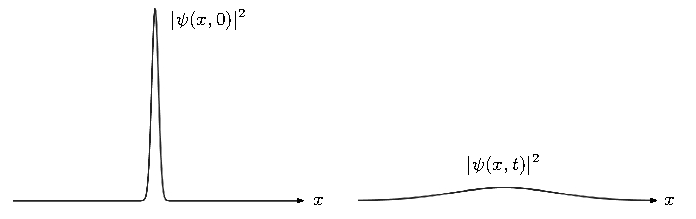
\includegraphics[width=.9\linewidth]{figures/ch03_fig01.pdf}
\caption{ユニタリーな時間発展に伴う、自由粒子のGaussian波束の確率密度$|\psi(x,t)|^2$のコヒーレントな拡散。}\label{fig:3.1}
\end{figure}

% 原文 p.117
\hypertarget{srcpage:117}{}\label{srcpage:117}
これは、波束の幅$\sigma$が
\begin{equation}
\sigma(t)=\sigma\left[1+\hbar^2t^2/(m^2\sigma^4)\right]^{1/2}
\tag{3.3}
\end{equation}
のように増大することを意味する。微視的粒子では、この拡散は非常に短い時間で起こる。例えば、Gaussian波束が電子の質量（$m\approx10^{-30}\,\mathrm{kg}$）をもつ粒子を記述し、その初期幅が$\sigma=1\,\text{\AA}$なら、ユニタリーな時間発展によって、わずか1秒のうちに波束の幅は$10^{16}\sigma=10^6\,\mathrm{m}$程度（実に1,000\,km！）にまで広がる。自由粒子の波動関数がコヒーレントに広がるこの効果は、狭い波束を粒子と結びつけようとする立場に重大な困難をもたらした。量子力学的な波束が直ちに巨視的距離にわたってコヒーレントに分散してしまうのであれば、明らかに空間的に明確な領域内にとどまる物体を、どうしてそのような波束と直接同一視できるだろうか。

孤立した自由粒子の場合には、波束と粒子の一対一対応を確立する試みが失敗したため、Schrödingerは粒子がポテンシャルを受ける状況に注意を向けた。特に、「微視的力学から巨視的力学への連続的移行」と題する有名な1926年の論文\footnote{ドイツ語の原題は ``Der stetige Übergang von der Mikro- zur Makromechanik.'' である。}\cite{ref157}では、量子調和振動子を例に取り、位置空間でのSchrödinger方程式の解（個々には空間的に広がった波を表す）を特定の仕方で線形結合すると、得られる波束は$t=0$で狭いだけでなく、その後のすべての時刻$t>0$でも狭いままにとどまり、そのピークが古典的な質点と同じように往復振動することを示した。

もちろんSchrödingerが発見したのは、量子調和振動子のコヒーレント状態、すなわち位相空間で古典軌道に従う最小不確定性波束であった。この成功に勇気づけられ、Schrödingerは次のように予測した\cite[p.~666]{ref157}。
\begin{quote}
ほぼ同じ方法で、大きな量子数をもつ楕円形のKepler軌道をたどり、水素原子中の電子の波動力学的な姿を表す波束も構成できるだろう。ただし、ここで扱った特に簡単な例に比べて、より多くの数学的困難に遭遇するかもしれない。\footnote{ドイツ語の原文は次のとおりである。``Es läßt sich mit Bestimmtheit voraussehen, daß man auf ganz ähnliche Weise auch die Wellengruppen konstruieren kann, welche auf hochquantigen Keplerellipsen umlaufen und das undulationsmechanische Bild des Wasserstoffelektrons sind; nur sind da die rechentechnischen Schwierigkeiten größer als in dem hier behandelten, ganz besonders einfachen Schulbeispiel.''}
\end{quote}

% 原文 p.118
\hypertarget{srcpage:118}{}\label{srcpage:118}
しかし、この評価（結局のところ、楽観的すぎた評価\footnote{Kepler軌道の場合には、理想化された量子調和振動子の例のような厳密なコヒーレント状態は得られない。別の興味深い例は、カオス的な回転運動を示すことが観測されているSaturnの衛星Hyperionである。カオス的運動は、古典軌道が初期の位相空間パラメータに指数関数的に敏感であることを意味するが、Heisenbergの不確定性原理のため、それらのパラメータを任意の精度で指定することはできない。したがって、Hyperionを記述する初めは狭い位相空間波束も、非常に速く広い空間領域へ広がる。実際、Zurek\cite{ref158}は、約20年のうちに、量子状態がこの衛星の主軸の巨視的に区別できる向きの、きわめて非局所的なコヒーレントな重ね合わせになると見積もった。したがって、惑星規模でさえコヒーレントな拡散の問題が生じうる。}であった）は、先に見いだされた核心的な問題、すなわち自由粒子を波束でどう記述するかという問題には触れていない。Schrödingerの論文の発表から数十年後、量子系が開いていることの重要性と、そこから生じるデコヒーレンス効果が理解されたこと\cite{ref004,ref005,ref006,ref008,ref009,ref012}により、自由粒子についてのSchrödinger方程式の予測と、すべての巨視的物体が局在して見えるという事実をどう両立させるかという困難の解決に、大きく近づいた。JoosとZehの先駆的論文\cite{ref007}は、詳細な模型と数値的結果を通じて、光子、空気分子、その他の環境粒子による遍在的な散乱が、極端に短い時間でコヒーレントな拡散を実効的に抑制する仕組みを示した。このデコヒーレンス過程によって得られる系の縮約密度行列は、位置空間の波束の（非真正な）アンサンブルを表し、その波束の幅は熱的de Broglie波長(2.114)へ向かって急速に減少する。

以下では、JoosとZehの原模型\cite{ref007}にさかのぼる、散乱によるデコヒーレンスの模型を調べる。現在では、文献\cite{ref007}に示された縮約密度行列の運動方程式の導出には微妙な誤りがあり、その結果、デコヒーレンス率が正しい値より$2\pi$倍大きくなることがわかっている\cite{ref159,ref160,ref161}。もちろん、論文が発表された1985年には、このような時間尺度の測定はいかなる実験でも手の届かないものに思われたため、JoosとZehの関心は、デコヒーレンスの時間尺度の簡単な見積もりにあった。しかし、この数年の実験技術の急速な進歩により、巨視的あるいは中間的な大きさの物体についてさえ、デコヒーレンスの時間尺度をきわめて精密に測定できるようになった（例えば、6.2節で述べるC$_{70}$分子の干渉実験を参照）。これらの測定は、前述の$2\pi$という因子程度の違いにも敏感であるため、定量的に正しい結果を与える環境散乱理論を用いることが重要になった。

さらに、JoosとZehの元の研究は、物体と散乱される環境粒子の波長の相対的な大きさについての仮定に基づいていた。この仮定を緩めた、より一般的な方法が、その後GallisとFleming\cite{ref162}によって与えられたが、導出における前述の誤りには対処しておらず、依然として余分な誤った因子$2\pi$が残った。

% 原文 p.119
\hypertarget{srcpage:119}{}\label{srcpage:119}
この誤りを修正し、デコヒーレンス率について正しい結果に到達した最初の導出は、Diósi\cite{ref159}によって与えられた。その数年後、HornbergerとSipe\cite{ref160}は環境散乱の問題を再検討し、Diósiのものとは大きく異なる洗練された方法を用いて正しい結果を得た。彼らの再評価は非常に注意深く徹底している一方で、かなり複雑でもある。最近、Adler\cite{ref161}は、ちょっとした工夫によって、はるかに簡単に正しい結果を得られることを示した。そのほか、例えばHalliwell\cite{ref163}やHornberger\cite{ref164,ref165}による導出もある。以下では、計算をできるだけ簡単に保ちながら正しい結果を得ることを目指して、主にHornbergerとSipe\cite{ref160}およびAdler\cite{ref161}の導出に従う。

本章の構成は次のとおりである。3.1節では散乱模型を導入する。3.2節では、空間的コヒーレンスの減衰を記述するデコヒーレンス因子の具体的な形を計算する。3.3節では二つの重要な極限、すなわち、系の空間的重ね合わせ状態を構成する二つの重心位置のコヒーレントな隔たりと比べて、環境の波長が短い場合（3.3.1節）と長い場合（3.3.2節）を扱う。3.4節では、この理論を光子の散乱（3.4.1節）と空気分子の散乱（3.4.2節）に適用する。最後に3.5節では、系の縮約密度行列の時間発展を調べることで、このような散乱によるデコヒーレンスから生じる具体的な運動を論じる。

\subsectionlink{散乱模型}
ある物体（系S）が、多数の環境粒子（環境E）を散乱する状況を考える（図3.2）。SとEは初め完全に無相関である、すなわち複合系SEの（純粋状態の）密度行列$\hat\rho$は$t=0$で因数分解されるという、通常の仮定を置く。
\begin{equation}
\hat\rho(0)=\hat\rho_{\mathrm S}(0)\otimes\hat\rho_{\mathrm E}(0).
\tag{3.4}
\end{equation}
まず一回の散乱事象を考え、それが系の密度行列$\hat\rho_{\mathrm S}$に及ぼす影響を調べよう（図3.3）。以下では、ごく基本的な量子力学の散乱理論を用いる。この主題の解説は、量子力学の教科書の多くにある（例えば文献\cite{ref058}の第7章）。しかし、他の文献を参照しなくても、読者はこの導出を追えるはずである。

重心位置$\bm x$をもつ系の初期状態を、固有値$\bm x$の位置固有状態$|\bm x\rangle$で表し、入射する環境粒子の初期状態を$|\chi_{\mathrm i}\rangle$と書こう。すると、散乱事象の効果は、散乱演算子$\hat S$（いわゆる「S行列」）の初期状態への作用によって、形式的に
\begin{equation}
|\bm x\rangle|\chi_{\mathrm i}\rangle\longrightarrow\hat S|\bm x\rangle|\chi_{\mathrm i}\rangle
\tag{3.5}
\end{equation}
と表せる。ここでは初期状態に対する分離可能性の仮定(3.4)を用いた。

\begin{figure}[htbp]\centering
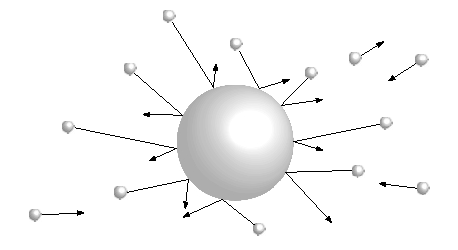
\includegraphics[width=.58\linewidth]{figures/ch03_fig02.pdf}
\caption{環境散乱。光子や空気分子などの粒子の集まりが、対象となる物体によって散乱される。}\label{fig:3.2}
\end{figure}
\begin{figure}[htbp]\centering
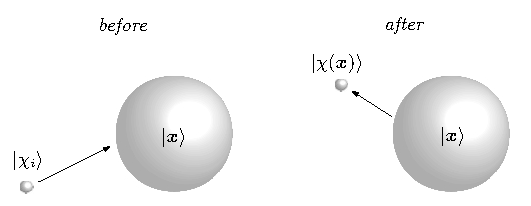
\includegraphics[width=.8\linewidth]{figures/ch03_fig03.pdf}
\caption{一回の散乱事象。初期状態$|\chi_{\mathrm i}\rangle$で記述される入射環境粒子が、静止した対象物によって弾性散乱される。対象物の重心状態は位置固有状態$|\bm x\rangle$で表される。散乱ポテンシャルの到達範囲は十分短く、物体と入射粒子の状態は初め無相関である。物体は散乱される環境粒子よりはるかに重く、散乱事象によって乱されないと仮定する。したがって、この相互作用は$|\bm x\rangle|\chi_{\mathrm i}\rangle\longrightarrow|\bm x\rangle|\chi(\bm x)\rangle$という発展をもたらす。$|\chi(\bm x)\rangle$は散乱粒子の終状態である［(3.12)も参照］。}\label{fig:3.3}
\end{figure}

% 原文 p.120
\hypertarget{srcpage:120}{}\label{srcpage:120}
自明なことを述べる危険を承知で付け加えれば、もちろん$|\chi_{\mathrm i}\rangle$は散乱物体の位置$\bm x$に依存しない。状態$|\bm x\rangle$は、原点に散乱中心がある状態$|\bm x=0\rangle$を、系の運動量演算子$\hat{\bm p}$の作用によって平行移動したものと考えられる。\footnote{この模型はデコヒーレンス時間尺度の具体的な数値の計算に用いるため、以下の導出では$\hbar$を残す。}
\begin{equation}
|\bm x\rangle=e^{-\mathrm i\hat{\bm p}\cdot\bm x/\hbar}|\bm x=0\rangle.
\tag{3.6}
\end{equation}
したがって(3.5)を次のように書き換えられる。
\begin{equation}
e^{-\mathrm i\hat{\bm p}\cdot\bm x/\hbar}|0\rangle|\chi_{\mathrm i}\rangle
\longrightarrow\hat S e^{-\mathrm i\hat{\bm p}\cdot\bm x/\hbar}|0\rangle|\chi_{\mathrm i}\rangle
=\hat S e^{-\mathrm i(\hat{\bm p}+\hat{\bm q})\cdot\bm x/\hbar}|0\rangle e^{\mathrm i\hat{\bm q}\cdot\bm x/\hbar}|\chi_{\mathrm i}\rangle.
\tag{3.7}
\end{equation}
% 原文 p.121
\hypertarget{srcpage:121}{}\label{srcpage:121}
ここで$\hat{\bm q}$は散乱される粒子の運動量演算子であり、したがって$\hat{\bm P}\equiv\hat{\bm p}+\hat{\bm q}$は複合系SEの運動量演算子である。

散乱相互作用が、複合系SEの空間的平行移動（すなわち演算子$\hat{\bm P}$が生成する平行移動）に対して不変である、
\begin{equation}
[\hat S,\hat{\bm P}]=0
\tag{3.8}
\end{equation}
と仮定すると、(3.7)の右辺の最初の指数関数を前に出して
\begin{equation}
\hat S|\bm x\rangle|\chi_{\mathrm i}\rangle
=e^{-\mathrm i(\hat{\bm p}+\hat{\bm q})\cdot\bm x/\hbar}\hat S|0\rangle e^{\mathrm i\hat{\bm q}\cdot\bm x/\hbar}|\chi_{\mathrm i}\rangle
\tag{3.9}
\end{equation}
を得る。

さらに進むため、ここで重要な仮定を置く。物体と散乱粒子の相互作用によって物体に反跳が生じないとするのである。これは、粒子が散乱事象によって実質的に乱されず、したがって散乱過程の唯一の帰結が、系と環境の間に量子的相関（もつれ）を作ることであることを意味する。

この仮定は、散乱系が散乱粒子よりはるかに重く、系の反跳効果を無視できる状況ではよい近似となる。微視的または中間的な大きさの粒子が巨視的物体によって散乱される場合には、これが成立すると期待できる。しかし、文献に挙げられた空間的デコヒーレンスの時間尺度の中には、散乱物体と散乱される環境粒子との質量比が1に近いか、あるいは1未満である散乱過程にも、この仮定を適用して計算したものがあることに注意しよう。一例は、空気分子の散乱によってデコヒーレンスを起こす小さな分子や自由電子の場合である\cite{ref166}。明らかに、この領域では無反跳の仮定が物理的に現実的であるとは期待できず、したがって（反跳を考慮する）Diósiの模型\cite{ref159}のような、より一般的な模型に頼るべきである。

以下の扱いでは、散乱物体が環境粒子よりはるかに重いとすることで、上の無反跳散乱の仮定を採用する。すると、系と環境の複合状態に対するS行列の作用は、系の重心状態$|\bm x\rangle$に影響を与えず、重心は位置$\bm x$にとどまる。したがって(3.7)をさらに計算できる。
\begin{equation}
\begin{aligned}
\hat S|\bm x\rangle|\chi_{\mathrm i}\rangle
&=e^{-\mathrm i(\hat{\bm p}+\hat{\bm q})\cdot\bm x/\hbar}|0\rangle\hat S_0e^{\mathrm i\hat{\bm q}\cdot\bm x/\hbar}|\chi_{\mathrm i}\rangle\\
&=e^{-\mathrm i\hat{\bm p}\cdot\bm x/\hbar}|0\rangle e^{-\mathrm i\hat{\bm q}\cdot\bm x/\hbar}\hat S_0e^{\mathrm i\hat{\bm q}\cdot\bm x/\hbar}|\chi_{\mathrm i}\rangle\\
&=|\bm x\rangle e^{-\mathrm i\hat{\bm q}\cdot\bm x/\hbar}\hat S_0e^{\mathrm i\hat{\bm q}\cdot\bm x/\hbar}|\chi_{\mathrm i}\rangle.
\end{aligned}\tag{3.10}
\end{equation}
ここでは散乱演算子$\hat S$に添字「0」を加え、散乱中心が原点にある散乱過程を特に指す演算子であることを示した。

% 原文 p.122
\hypertarget{srcpage:122}{}\label{srcpage:122}
(3.10)の最後の行を用いて、平行移動された散乱演算子
\begin{equation}
\hat S_{\bm x}\equiv e^{-\mathrm i\hat{\bm q}\cdot\bm x/\hbar}\hat S_0e^{\mathrm i\hat{\bm q}\cdot\bm x/\hbar}
\tag{3.11}
\end{equation}
を定義できる。これは散乱中心が位置$\bm x$にある散乱を記述する。まとめると、散乱相互作用は
\begin{equation}
|\bm x\rangle|\chi_{\mathrm i}\rangle\longrightarrow\hat S|\bm x\rangle|\chi_{\mathrm i}\rangle
=|\bm x\rangle\hat S_{\bm x}|\chi_{\mathrm i}\rangle\equiv|\bm x\rangle|\chi(\bm x)\rangle
\tag{3.12}
\end{equation}
と与えられる。ここで$|\chi(\bm x)\rangle$は、$\bm x$で散乱された環境粒子の終状態の略記である。(3.12)から、散乱過程は、系の重心位置を記述する状態$|\bm x\rangle$と、散乱中心の位置$\bm x$についての経路情報を符号化した粒子の終状態$|\chi(\bm x)\rangle$の間に相関を確立する、測定に似た相互作用と考えられることがわかる。

(3.12)より、散乱過程は初期の複合密度行列
\begin{equation}
\hat\rho(0)=\hat\rho_{\mathrm S}(0)\otimes\hat\rho_{\mathrm E}(0)
=\int\mathrm d\bm x\int\mathrm d\bm x'\,\rho_{\mathrm S}(\bm x,\bm x',0)|\bm x\rangle\langle\bm x'|\otimes|\chi_{\mathrm i}\rangle\langle\chi_{\mathrm i}|
\tag{3.13}
\end{equation}
を密度行列
\begin{equation}
\hat\rho=\int\mathrm d\bm x\int\mathrm d\bm x'\,\rho_{\mathrm S}(\bm x,\bm x',0)|\bm x\rangle\langle\bm x'|\otimes|\chi(\bm x)\rangle\langle\chi(\bm x')|
\tag{3.14}
\end{equation}
に変換する。(2.50)を用いると、対応する系の最終縮約密度行列$\hat\rho_{\mathrm S}$は
\begin{equation}
\hat\rho_{\mathrm S}=\operatorname{Tr}_{\mathrm E}\hat\rho
=\int\mathrm d\bm x\int\mathrm d\bm x'\,\rho_{\mathrm S}(\bm x,\bm x',0)|\bm x\rangle\langle\bm x'|\langle\chi(\bm x')|\chi(\bm x)\rangle
\tag{3.15}
\end{equation}
と与えられる。したがって、位置基底で表すと、散乱による縮約密度行列の発展は
\begin{equation}
\rho_{\mathrm S}(\bm x,\bm x',0)\longrightarrow\rho_{\mathrm S}(\bm x,\bm x',0)\langle\chi(\bm x')|\chi(\bm x)\rangle
\tag{3.16}
\end{equation}
とまとめられる。散乱事象による空間的コヒーレンスの局所的抑制は、散乱粒子の相対状態の重なり$\langle\chi(\bm x')|\chi(\bm x)\rangle$によって定量化されることがわかる（2.6.3節と2.7節での一般的な議論も参照）。次に、この重なりの時間依存性を計算しよう。
\subsectionlink{デコヒーレンス因子の計算}
先に進むため、散乱演算子$\hat S_0$を、別の演算子$\hat T$（「T行列」）を用いて形式的に
\begin{equation}
\hat S_0=\hat I+\mathrm i\hat T
\tag{3.17}
\end{equation}
と書こう。
% 原文 p.123
\hypertarget{srcpage:123}{}\label{srcpage:123}
T行列は標準的な量子力学の散乱理論でよく知られている（例えば文献\cite{ref058}）。ここでこれを用いるのは、散乱粒子の運動量固有基底$\{|\bm q\rangle\}$における行列要素を、散乱振幅$f(\bm q,\bm q')$によって、都合よく
\begin{equation}
\langle\bm q|\hat T|\bm q'\rangle=\frac{\mathrm i}{2\pi\hbar q}\delta(q-q')f(\bm q,\bm q')
=\frac{\mathrm i}{2\pi\hbar m}\delta(E-E')f(\bm q,\bm q')
\tag{3.18}
\end{equation}
と定義できるからである。ここで$m$は環境粒子の質量、$q=|\bm q|$である。項$\delta(E-E')$は、反跳のない弾性散乱という仮定が要求するエネルギー保存を保証する。$|f(\bm q,\bm q')|^2$は実験で測定できる量、すなわち散乱過程の微分断面積$\mathrm d\sigma/\mathrm d\Omega$であり、
\begin{equation}
\frac{\mathrm d\sigma}{\mathrm d\Omega}\equiv\frac{\text{散乱流束}}{\text{入射流束}}
\tag{3.19}
\end{equation}
と定義されることに注意しよう。

散乱演算子$\hat S_0$はユニタリーであり、
\begin{equation}\hat S_0\hat S_0^{\dagger}=\hat I,\tag{3.20}\end{equation}
T行列の定義(3.17)から次の関係を得る。
\begin{equation}\hat T\hat T^{\dagger}+\mathrm i(\hat T-\hat T^{\dagger})=0.\tag{3.21}\end{equation}
この結果は後で役に立つ。

環境状態の表式(3.12)を用いると、重なり$\langle\chi(\bm x')|\chi(\bm x)\rangle$は
\begin{equation}
\langle\chi(\bm x')|\chi(\bm x)\rangle=\langle\chi_{\mathrm i}|\hat S_{\bm x'}^{\dagger}\hat S_{\bm x}|\chi_{\mathrm i}\rangle
\tag{3.22}
\end{equation}
と与えられる。明らかにこの表式は、平行移動された散乱演算子(3.11)の積$\hat S_{\bm x'}^{\dagger}\hat S_{\bm x}$の、入射環境粒子の（純粋）状態$|\chi_{\mathrm i}\rangle$における期待値に等しい（混合状態への一般化は容易である）。したがって、トレース則(2.17)を用いれば、(3.22)を同値な形
\begin{equation}
\langle\chi(\bm x')|\chi(\bm x)\rangle=\operatorname{Tr}_{\mathrm E}\{\hat\rho_{\mathrm E}(0)\hat S_{\bm x'}^{\dagger}\hat S_{\bm x}\}
\tag{3.23}
\end{equation}
に書き換えられる。ここで$\hat\rho_{\mathrm E}(0)=|\chi_{\mathrm i}\rangle\langle\chi_{\mathrm i}|$である。これがこれから計算する対象の表式である。まず、環境粒子が箱型規格化の体積$V$に制限されていると仮定しよう。文献\cite{ref160}に従い、体積$V$で規格化された運動量固有ケット$|\widetilde{\bm q}\rangle$を
\begin{equation}
|\widetilde{\bm q}\rangle\equiv\left[\frac{(2\pi\hbar)^3}{V}\right]^{1/2}|\bm q\rangle
\tag{3.24}
\end{equation}
と定義する。

% 原文 p.124
\hypertarget{srcpage:124}{}\label{srcpage:124}
ケット$|\widetilde{\bm q}\rangle$は、
\begin{equation}
\sum_{\bm q\in Q_V}|\widetilde{\bm q}\rangle\langle\widetilde{\bm q}|=\hat I_V
\tag{3.25}
\end{equation}
という意味で、体積$V$上の正規直交基底を構成する。ここで$Q_V$は、体積$V$において周期的境界条件を満たす波動関数の空間に対応するすべての運動量の集合であり、$\hat I_V$はこの空間の恒等演算子である。

すると、環境粒子の初期密度行列$\hat\rho_{\mathrm E}(0)$を、規格化された運動量固有状態$|\widetilde{\bm q}\rangle$のアンサンブルによって
\begin{equation}
\hat\rho_{\mathrm E}(0)=\frac{(2\pi\hbar)^3}{V}\sum_{\bm q\in Q_V}\mu(\bm q)|\widetilde{\bm q}\rangle\langle\widetilde{\bm q}|
\tag{3.26}
\end{equation}
と展開できる。$\mu(\bm q)$は運動量空間の密度である。この展開を用いる大きな利点は、演算子$\hat T$［(3.17)、(3.18)参照］が、全空間の運動量基底$\{|\bm q\rangle\}$で対角的であり、したがって適切に規格化された体積$V$の基底$\{|\widetilde{\bm q}\rangle\}$でも対角的であるということである。

この性質により、重なり$\langle\chi(\bm x')|\chi(\bm x)\rangle$［(3.23)参照］をかなり直接的に計算できる。(3.23)に環境状態の展開(3.26)を用いると、まず
\begin{equation}
\begin{aligned}
\langle\chi(\bm x')|\chi(\bm x)\rangle
&=\frac{(2\pi\hbar)^3}{V}\sum_{\bm q\in Q_V}\mu(\bm q)\langle\widetilde{\bm q}|\hat S_{\bm x'}^{\dagger}\hat S_{\bm x}|\widetilde{\bm q}\rangle\\
&=\frac{(2\pi\hbar)^3}{V}\sum_{\bm q\in Q_V}\mu(\bm q)\langle\widetilde{\bm q}|e^{-\mathrm i\hat{\bm q}\cdot\bm x'/\hbar}\hat S_0^{\dagger}
e^{-\mathrm i\hat{\bm q}\cdot(\bm x-\bm x')/\hbar}\hat S_0e^{\mathrm i\hat{\bm q}\cdot\bm x/\hbar}|\widetilde{\bm q}\rangle\\
&=\frac{(2\pi\hbar)^3}{V}\sum_{\bm q\in Q_V}\mu(\bm q)e^{\mathrm i\bm q\cdot(\bm x-\bm x')/\hbar}
\langle\widetilde{\bm q}|\hat S_0^{\dagger}e^{-\mathrm i\hat{\bm q}\cdot(\bm x-\bm x')/\hbar}\hat S_0|\widetilde{\bm q}\rangle
\end{aligned}\tag{3.27}
\end{equation}
を得る。次に、$\hat S_0=\hat I+\mathrm i\hat T$［(3.17)参照］および関係(3.21)を用いると、これは
\begin{equation}
\begin{aligned}
&\langle\chi(\bm x')|\chi(\bm x)\rangle\\
&=\frac{(2\pi\hbar)^3}{V}\sum_{\bm q\in Q_V}\mu(\bm q)e^{\mathrm i\bm q\cdot(\bm x-\bm x')/\hbar}
\langle\widetilde{\bm q}|(\hat I-\mathrm i\hat T^{\dagger})e^{-\mathrm i\hat{\bm q}\cdot(\bm x-\bm x')/\hbar}(\hat I+\mathrm i\hat T)|\widetilde{\bm q}\rangle\\
&=\frac{(2\pi\hbar)^3}{V}\sum_{\bm q\in Q_V}\mu(\bm q)
\left[1-\langle\widetilde{\bm q}|\hat T\hat T^{\dagger}|\widetilde{\bm q}\rangle
+e^{\mathrm i\bm q\cdot(\bm x-\bm x')/\hbar}\langle\widetilde{\bm q}|\hat T^{\dagger}e^{-\mathrm i\hat{\bm q}\cdot(\bm x-\bm x')/\hbar}\hat T|\widetilde{\bm q}\rangle\right]
\end{aligned}\tag{3.28}
\end{equation}
となる。演算子$\hat T$が運動量演算子と可換なので［(3.18)参照］、最後の行の角括弧内の第2項に付随する指数関数はすべて消えている。

% 原文 p.125
\hypertarget{srcpage:125}{}\label{srcpage:125}
運動量固有状態$|\widetilde{\bm q}\rangle$の完全系［(3.25)参照］を挿入し、さらに(3.18)を用いて、(3.28)の最後の行の和に含まれる第2項と第3項を計算しよう。すると
\begin{equation}
\begin{aligned}
&\langle\chi(\bm x')|\chi(\bm x)\rangle\\
&=\frac{(2\pi\hbar)^3}{V}\sum_{\bm q\in Q_V}\mu(\bm q)
\left[1-\sum_{\bm q'\in Q_V}\left(1-e^{\mathrm i(\bm q-\bm q')\cdot(\bm x-\bm x')/\hbar}\right)
\left|\langle\widetilde{\bm q}|\hat T|\widetilde{\bm q}'\rangle\right|^2\right]
\end{aligned}\tag{3.29}
\end{equation}
を得る。ここで、通常の変換関係
\begin{equation}
\frac{(2\pi\hbar)^3}{V}\sum_{\bm q\in Q_V}\longrightarrow\int\mathrm d\bm q
\tag{3.30}
\end{equation}
に従って和を積分に置き換え、運動量状態$|\widetilde{\bm q}\rangle$の連続極限へ移る。$\int\mathrm d\bm q\,\mu(\bm q)=1$と定義(3.24)を用いると、(3.29)は
\begin{equation}
\begin{aligned}
\langle\chi(\bm x')|\chi(\bm x)\rangle
=1-&\int\mathrm d\bm q\,\mu(\bm q)\frac{(2\pi\hbar)^3}{V}\int\mathrm d\bm q'\,
\left(1-e^{\mathrm i(\bm q-\bm q')\cdot(\bm x-\bm x')/\hbar}\right)
|\langle\bm q|\hat T|\bm q'\rangle|^2
\end{aligned}\tag{3.31}
\end{equation}
となる。

Adlerの方法\cite{ref161}に従い、散乱過程で経過した時間を表す時間パラメータ$T$を導入しよう。すると(3.16)と(3.31)から、縮約密度行列の発展は
\begin{equation}
\begin{aligned}
&\rho_{\mathrm S}(\bm x,\bm x',T)-\rho_{\mathrm S}(\bm x,\bm x',0)=-\rho_{\mathrm S}(\bm x,\bm x',0)\\
&\quad\times\int\mathrm d\bm q\,\mu(\bm q)\frac{(2\pi\hbar)^3}{V}\int\mathrm d\bm q'\,
\left(1-e^{\mathrm i(\bm q-\bm q')\cdot(\bm x-\bm x')/\hbar}\right)|\langle\bm q|\hat T|\bm q'\rangle|^2
\end{aligned}\tag{3.32}
\end{equation}
と書ける。(3.32)を書く際、物体の自由発展の特徴的な時間尺度は散乱事象の平均間隔よりはるかに長く、区間$T$内での物体の密度行列の変化は散乱事象のみから生じると仮定したことに注意しよう。

次に、この式に現れる行列要素の二乗$|\langle\bm q|\hat T|\bm q'\rangle|^2$を計算する。(3.18)の形
\begin{equation}
\langle\bm q|\hat T|\bm q'\rangle=\frac{\mathrm i}{2\pi\hbar m}\delta(E-E')f(\bm q,\bm q')
\tag{3.33}
\end{equation}
を用いると、計算すべきものは
\begin{equation}
|\langle\bm q|\hat T|\bm q'\rangle|^2=\frac{1}{(2\pi\hbar m)^2}\delta^2(E-E')|f(\bm q,\bm q')|^2
\tag{3.34}
\end{equation}
である。

% 原文 p.126
\hypertarget{srcpage:126}{}\label{srcpage:126}
エネルギーのデルタ関数の二乗$\delta^2(E-E')$は、時間依存摂動論における遷移確率についてのFermiの黄金律を導く際によく現れる（例えば文献\cite{ref167}の第18章を参照）。実際、行列要素$|\langle\bm q|\hat T|\bm q'\rangle|^2$は、明らかに散乱による遷移$|\bm q\rangle\longrightarrow|\bm q'\rangle$の確率にほかならない。

そこで、Adlerが提案した方法\cite{ref161}（Fermiの黄金律の導出に通常用いられる方法に似ている）に従い、エネルギーのデルタ関数のFourier積分表示
\begin{equation}
\delta(E-E')=\lim_{T\to\infty}\frac{1}{2\pi\hbar}\int_{-T/2}^{T/2}\mathrm dt\,e^{\mathrm i(E-E')t/\hbar}
\tag{3.35}
\end{equation}
を用いて、その二乗を扱える。これにより
\begin{equation}
\begin{aligned}
\delta^2(E-E')
&=\delta(E-E')\lim_{T\to\infty}\frac{1}{2\pi\hbar}\int_{-T/2}^{T/2}\mathrm dt\,e^{\mathrm i(E-E')t/\hbar}\\
&=\delta(E-E')\lim_{T\to\infty}\frac{1}{2\pi\hbar}\int_{-T/2}^{T/2}\mathrm dt\\
&=\delta(E-E')\lim_{T\to\infty}\frac{T}{2\pi\hbar}
\end{aligned}\tag{3.36}
\end{equation}
と書ける。第2行では、積分の前にある最初のデルタ関数が、$E=E'$でなければゼロになることを用いた。

Fermiの黄金律の一般的導出では、パラメータ$T$は、相互作用が「入っている」時間区間と解釈できる。(3.36)は、十分大きな$T$に対して遷移確率が$T$にほぼ比例して増加することを示す。したがって、$T$を一回の散乱事象が起こる典型的な所要時間よりはるかに長い時間区間とすれば、(3.36)を
\begin{equation}
\delta^2(E-E')=\delta(E-E')\frac{T}{2\pi\hbar}
=\delta(q-q')\frac{m}{q}\frac{T}{2\pi\hbar}
\tag{3.37}
\end{equation}
と書ける。さらに、$T$は、多数の粒子の散乱によって中心粒子に生じる特徴的なデコヒーレンス時間よりも十分短いと仮定する。一般に、顕著な空間的デコヒーレンスを生じるには物体と環境粒子との多数回の衝突が必要なので、このような$T$の領域を選ぶことは妥当である。

次に(3.37)を(3.34)で用い、得られた表式を(3.32)へ代入する。(3.37)のデルタ関数$\delta(q-q')$は、$|\bm q'|=|\bm q|$という運動量の保存を課す。$\mathrm d\bm q'\equiv q^2\mathrm d\hat{\bm n}'$と書くと（$\mathrm d\hat{\bm n}'$は運動量空間の立体角の微分）、容易に
\begin{equation}
\begin{aligned}
&\rho_{\mathrm S}(\bm x,\bm x',T)-\rho_{\mathrm S}(\bm x,\bm x',0)=-\rho_{\mathrm S}(\bm x,\bm x',0)\\
&\quad\times\frac{T}{V}\int\mathrm d\bm q\,\mu(\bm q)v(q)\int\mathrm d\hat{\bm n}'
\left(1-e^{\mathrm i(\bm q-q\hat{\bm n}')\cdot(\bm x-\bm x')/\hbar}\right)|f(\bm q,q\hat{\bm n}')|^2
\end{aligned}\tag{3.38}
\end{equation}
を得る。

% 原文 p.127
\hypertarget{srcpage:127}{}\label{srcpage:127}
ここで$v(q)$は、運動量$q$をもつ粒子の速さを表す。質量をもつ粒子の散乱では$v(q)=q/m$、光子など質量のない粒子の散乱では$v(q)=c$であり、$c$は光速である。

(3.38)は一回の散乱事象の効果を記述する。$N$回の独立な散乱事象の集まりは、(3.38)の右辺の積分に$N$を掛けるだけで表せる。このとき$N/V$が環境粒子の全数密度となる。簡単のため、入射粒子は空間的に等方分布している、すなわち初期のすべての方向$\bm q/|\bm q|$は等確率であると仮定しよう。すると、運動量の確率分布$\mu(\bm q)$を
\begin{equation}
\mu(\bm q)\equiv\frac{1}{4\pi}\left(\frac{N}{V}\right)^{-1}\varrho(q)\,\mathrm dq\,\mathrm d\hat{\bm n}
\tag{3.39}
\end{equation}
と書ける。前の因子は、$\int\mathrm dq\,\varrho(q)=N/V$となるように選んだ（$\int\mathrm d\bm q\,\mu(\bm q)=1$を思い出そう）。すなわち$\varrho(q)$は、運動量の大きさが$q$に等しい入射粒子の数密度を表す。

(3.38)を$T$で割り、小さな$T$の微分極限を取ると、縮約密度行列の時間発展についての最終結果
\begin{equation}
\frac{\partial\rho_{\mathrm S}(\bm x,\bm x',t)}{\partial t}=-F(\bm x-\bm x')\rho_{\mathrm S}(\bm x,\bm x',t)
\tag{3.40}
\end{equation}
を得る。デコヒーレンス因子$F(\bm x-\bm x')$は
\begin{equation}
F(\bm x-\bm x')=\int\mathrm dq\,\varrho(q)v(q)\int\frac{\mathrm d\hat{\bm n}\,\mathrm d\hat{\bm n}'}{4\pi}
\left(1-e^{\mathrm iq(\hat{\bm n}-\hat{\bm n}')\cdot(\bm x-\bm x')/\hbar}\right)|f(q\hat{\bm n},q\hat{\bm n}')|^2
\tag{3.41}
\end{equation}
で与えられる。(3.40)より、$F(\bm x-\bm x')$は局在化率として働き、二つの位置$\bm x$、$\bm x'$の間の空間的コヒーレンスが局所的に抑制される特徴的なデコヒーレンス率を表すことがわかる。

(3.40)と(3.41)が主な結果である。対象物によって散乱される入射粒子の集まりが、物体の位置密度行列の干渉項（非対角項）に及ぼす影響を定量化する表式を得た。散乱断面積$|f(q\hat{\bm n},q\hat{\bm n}')|^2$の形はまだ指定していないので、この表式はかなり一般的といえる。

(3.40)、(3.41)の導出に用いた仮定をまとめよう。
\begin{enumerate}
\item 系と環境の間に初期相関がない［(3.4)参照］。この仮定は、事実上すべてのデコヒーレンス模型で用いられる（第5章も参照）。
\item 散乱相互作用は、物体と環境の複合系の平行移動に対して不変である［(3.8)参照］。
\item 物体の重心状態は、散乱事象によって乱されない。
\item 散乱率は、系自身のHamiltonianが誘起する系の状態変化の特徴的な率より、はるかに大きい。
\item 入射粒子の方向分布は等方的である［(3.39)参照］。
\end{enumerate}
% 原文 p.128
\hypertarget{srcpage:128}{}\label{srcpage:128}
これらの仮定の大部分はかなり穏当であり、ここで模型化しようとしている物理的状況、すなわち単位時間当たり多数の微視的または中間的な大きさの粒子が巨視的物体によって散乱される状況では、十分に正当化できる。最も制約が強い可能性があるのは、無反跳の仮定（上の仮定3）である。すでに述べたように、この仮定のために、散乱物体と散乱される環境粒子の質量が同程度の状況では、局在化模型は非現実的になる。
\subsectionlink{完全な経路識別と部分的な経路識別}
対象物が、距離$\Delta x=|\bm x-\bm x'|$だけ離れた、よく局在した二つの波束のコヒーレントな重ね合わせで記述されているとしよう。結果(3.40)、(3.41)によれば、この重ね合わせは、環境散乱によってどのくらい速くデコヒーレンスを起こすだろうか。この問いに答えるため、二つの極限を論じる。各散乱粒子が隔たり$\Delta x$を完全に識別する短波長極限と、環境に顕著な量の経路情報が符号化され、それによってこの隔たりが識別されるまでに、多数の散乱事象を要する長波長極限である。

\subsubsectionlink{短波長極限}
まず、散乱粒子の典型的な波長$\lambda_0$が、コヒーレントな隔たり$\Delta x=|\bm x-\bm x'|$よりはるかに短い状況、$\lambda_0\ll\Delta x$を考えよう。このとき、粒子はこの隔たりを十分によく識別でき、したがって最大の経路情報を持ち去り、一回の散乱事象当たり最大のデコヒーレンスを系に引き起こすと期待される。

この予想が本当に正しいか確かめるため、$F(\bm x-\bm x')$の表式(3.41)を見よう。de Broglieの関係によれば、波長$\lambda_0$は運動量$q_0=2\pi\hbar/\lambda_0$に対応するので、$\lambda_0\ll\Delta x$ならば$q_0\Delta x/\hbar\gg1$である。したがって、(3.41)の右辺の積分に含まれる指数関数は非常に速く振動し、平均すれば定数項1に比べて積分に寄与しない。この極限では
\begin{equation}
F(\bm x-\bm x')=\int\mathrm dq\,\varrho(q)v(q)\int\frac{\mathrm d\hat{\bm n}\,\mathrm d\hat{\bm n}'}{4\pi}|f(q\hat{\bm n},q\hat{\bm n}')|^2.
\tag{3.42}
\end{equation}
% 原文 p.129
\hypertarget{srcpage:129}{}\label{srcpage:129}
積分
\begin{equation}
\int\mathrm d\hat{\bm n}'\,|f(q\hat{\bm n},q\hat{\bm n}')|^2
\tag{3.43}
\end{equation}
は、運動量$\bm q=q\hat{\bm n}$に対する全断面積に等しい。次の$\mathrm d\hat{\bm n}$についての積分は$\bm q$の可能なすべての方向$\hat{\bm n}$の平均を取り、
\begin{equation}
\int\frac{\mathrm d\hat{\bm n}\,\mathrm d\hat{\bm n}'}{4\pi}|f(q\hat{\bm n},q\hat{\bm n}')|^2=\sigma_{\mathrm{tot}}(q)
\tag{3.44}
\end{equation}
を得る。$\sigma_{\mathrm{tot}}(q)$は、方向を問わず運動量$q$に対する全断面積である。したがって(3.42)は
\begin{equation}
F(\bm x-\bm x')=\int\mathrm dq\,\varrho(q)v(q)\sigma_{\mathrm{tot}}(q)
\tag{3.45}
\end{equation}
となる。この積分が全散乱率$\Gamma_{\mathrm{tot}}$に等しいことに気づけば、さらに簡単に
\begin{equation}F(\bm x-\bm x')=\Gamma_{\mathrm{tot}}\tag{3.46}\end{equation}
とできる。

この結果は、隔たり$\Delta x$をいくら大きくしても、デコヒーレンス率には上限があることを意味する。これは当然ながら、まったく妥当な結果である。任意の隔たり$\Delta x$に対して、その隔たりの完全な識別を可能にし、したがって最大の空間的デコヒーレンスをもたらす環境粒子の波長が存在する。それ以上隔たりを大きくしても、さらに強いデコヒーレンスをもたらすことはできない。

(3.46)を(3.40)に代入すると、系の縮約密度行列の非対角要素$\rho_{\mathrm S}(\bm x,\bm x')$、$\bm x\ne\bm x'$は
\begin{equation}
\frac{\partial\rho_{\mathrm S}(\bm x,\bm x',t)}{\partial t}=-\Gamma_{\mathrm{tot}}\rho_{\mathrm S}(\bm x,\bm x',t)
\tag{3.47}
\end{equation}
と変化する。系の内部運動を無視できる短い時間区間では、干渉項の時間発展はしたがって
\begin{equation}
\rho_{\mathrm S}(\bm x,\bm x',t)=\rho_{\mathrm S}(\bm x,\bm x',0)e^{-\Gamma_{\mathrm{tot}}t}
\tag{3.48}
\end{equation}
と与えられる。これは、最大のデコヒーレンスの極限では、空間的な干渉項が、全散乱率$\Gamma_{\mathrm{tot}}$によって定まる率で指数関数的に抑制されることを示す。

% 原文 p.130
\hypertarget{srcpage:130}{}\label{srcpage:130}
\subsubsectionlink{長波長極限}
次に、入射粒子の典型的な波長$\lambda_0$が、コヒーレントな隔たり$\Delta x=|\bm x-\bm x'|$よりはるかに長い、反対の極限を考えよう。この場合、個々の散乱粒子は隔たり$\Delta x$を識別できず、不十分な量の経路情報しか持ち去らない。したがって、物体に顕著な空間的局在化を生じさせるには、多数の散乱事象が必要になると予想される。\footnote{JoosとZehの元の導出\cite{ref007}は、初めから$\lambda_0\gg\Delta x$の極限を仮定していた［文献\cite{ref007}の式(3.45)に続くコメントを参照］。したがって、その目的は局在化率の慎重な下限評価を与えることにあった。}

仮定$\lambda_0\gg\Delta x$（同値に、運動量の典型値$q_0$に対して$q_0\Delta x/\hbar\ll1$）が、$F(\bm x-\bm x')$の表式(3.41)に及ぼす影響を調べよう。(3.41)の指数関数を、その引数$q(\hat{\bm n}-\hat{\bm n}')(\bm x-\bm x')$について1次まで展開する。すなわち
\begin{equation}
\begin{aligned}
1-e^{\mathrm iq(\hat{\bm n}-\hat{\bm n}')\cdot(\bm x-\bm x')/\hbar}
\approx&-\frac{\mathrm i}{\hbar}q(\hat{\bm n}-\hat{\bm n}')\cdot(\bm x-\bm x')\\
&+\frac{q^2}{2\hbar^2}[(\hat{\bm n}-\hat{\bm n}')\cdot(\bm x-\bm x')]^2.
\end{aligned}\tag{3.49}
\end{equation}
この展開の第1項は、$F(\bm x-\bm x')$の表式(3.41)の積分に寄与しない。これは次のことから直ちにわかる。$f(q\hat{\bm n},q\hat{\bm n}')=f^*(q\hat{\bm n}',q\hat{\bm n})$［(3.18)参照］なので、$|f(q\hat{\bm n},q\hat{\bm n}')|^2=|f(q\hat{\bm n}',q\hat{\bm n})|^2$である。したがって、$(\hat{\bm n},\hat{\bm n}')$について奇である関数$(\hat{\bm n}-\hat{\bm n}')\cdot(\bm x-\bm x')$と、これらについて偶である関数$|f(q\hat{\bm n},q\hat{\bm n}')|^2$との積が現れる。$\bm q$と$\bm q'$のすべての方向$\hat{\bm n}$、$\hat{\bm n}'$について積分すると、この積による寄与は平均してゼロになる。

$q_0\Delta x/\hbar\ll1$の極限における$F(\bm x-\bm x')$の表式は、したがって
\begin{equation}
F(\bm x-\bm x')=\int\mathrm dq\,\varrho(q)v(q)q^2\int\frac{\mathrm d\hat{\bm n}\,\mathrm d\hat{\bm n}'}{8\pi\hbar^2}
[(\hat{\bm n}-\hat{\bm n}')\cdot(\bm x-\bm x')]^2|f(q\hat{\bm n},q\hat{\bm n}')|^2
\tag{3.50}
\end{equation}
となる。散乱中心（したがって座標系）の向きが散乱過程に影響を与えないと仮定すれば、この式をさらに簡単にできる。第一に、これにより、項$[(\hat{\bm n}-\hat{\bm n}')\cdot(\bm x-\bm x')]^2$を、すべての方向$(\bm x-\bm x')$について平均できる。この平均は
\begin{equation}
\begin{aligned}
(\bm x-\bm x')^2\frac13\sum_{i=x,y,z}[(\hat{\bm n}-\hat{\bm n}')\cdot\hat{\bm i}]^2
&=\frac13(\bm x-\bm x')^2(\hat{\bm n}-\hat{\bm n}')^2\\
&=\frac23(\bm x-\bm x')^2(1-\hat{\bm n}\cdot\hat{\bm n}')\\
&=\frac23(\bm x-\bm x')^2(1-\cos\Theta)
\end{aligned}\tag{3.51}
\end{equation}
と与えられる。
% 原文 p.131
\hypertarget{srcpage:131}{}\label{srcpage:131}
ここで$\Theta$は、散乱粒子の入射軌道と出射軌道のなす角である。したがって
\begin{equation}
F(\bm x-\bm x')=(\bm x-\bm x')^2\int\mathrm dq\,\varrho(q)v(q)q^2\frac{2}{3\hbar^2}
\int\frac{\mathrm d\hat{\bm n}\,\mathrm d\hat{\bm n}'}{8\pi}(1-\cos\Theta)|f(q\hat{\bm n},q\hat{\bm n}')|^2.
\tag{3.52}
\end{equation}
第二に、断面積$|f(q\hat{\bm n},q\hat{\bm n}')|^2$は等方的、すなわち運動量の大きさ$q$と散乱角$\Theta$のみに依存するとしてよい。このとき、角度積分の一部を実行して(3.52)をさらに簡単にし、
\begin{equation}
F(\bm x-\bm x')=(\bm x-\bm x')^2\int\mathrm dq\,\varrho(q)v(q)q^2\frac{2\pi}{3\hbar^2}
\int\mathrm d\cos\Theta\,(1-\cos\Theta)|f(q,\cos\Theta)|^2
\tag{3.53}
\end{equation}
を得る。角度による重み$(1-\cos\Theta)$を除けば、第2の積分は、散乱過程の全断面積$\sigma_{\mathrm{tot}}(q)$の表式(3.44)と似ている。そこで
\begin{equation}
\sigma_{\mathrm{eff}}(q)\equiv\frac{2\pi}{3}\int\mathrm d\cos\Theta\,(1-\cos\Theta)|f(q,\cos\Theta)|^2
\tag{3.54}
\end{equation}
を散乱相互作用の実効断面積と解釈しよう。これは、その結果、全断面積$\sigma_{\mathrm{tot}}(q)$と同程度の大きさとなる。

次に、物体の縮約密度行列の干渉項$\rho_{\mathrm S}(\bm x,\bm x')$、$\bm x\ne\bm x'$の時間依存性を調べよう。(3.40)に戻り、(3.53)、(3.54)を用いると、散乱による縮約密度行列の変化は
\begin{equation}
\frac{\partial\rho_{\mathrm S}(\bm x,\bm x',t)}{\partial t}=-\Lambda(\bm x-\bm x')^2\rho_{\mathrm S}(\bm x,\bm x',t)
\tag{3.55}
\end{equation}
となる。ここでは、相互作用の物理的な詳細をまとめた散乱定数
\begin{equation}
\Lambda\equiv\int\mathrm dq\,\varrho(q)v(q)\frac{q^2}{\hbar^2}\sigma_{\mathrm{eff}}(q)
\tag{3.56}
\end{equation}
を導入した。

系の内部運動に比べて短い時間尺度では、(3.55)より、散乱事象は、時間と隔たりの二乗$(\Delta x)^2=(\bm x-\bm x')^2$に対して指数関数的に強まる非対角項の抑制、
\begin{equation}
\rho_{\mathrm S}(\bm x,\bm x',t)=\rho_{\mathrm S}(\bm x,\bm x',0)e^{-\Lambda(\Delta x)^2t}
\tag{3.57}
\end{equation}
をもたらす。散乱定数$\Lambda$は、与えられた距離$\Delta x$にわたる空間的コヒーレンスが抑制される率を定量化することがわかる。このことから、(3.57)は、デコヒーレンス時間尺度$\tau_{\Delta x}$を
\begin{equation}
\tau_{\Delta x}=\frac{1}{\Lambda(\Delta x)^2}
\tag{3.58}
\end{equation}
と導入する動機を与える。
% 原文 p.132
\hypertarget{srcpage:132}{}\label{srcpage:132}
これは、距離$\Delta x$にわたる空間的コヒーレンスを$e$分の1に減衰させるために必要な特徴的時間である。その逆数$\tau_{\Delta x}^{-1}$は、したがってデコヒーレンス率として働く。

環境の波長が隔たり$\Delta x$よりはるかに短いと仮定した、反対の極限で得られた結果(3.48)と対照的に、(3.58)では、減衰は$\Delta x$に陽に、しかも強く依存する。この違いは先の議論からかなり容易に理解できる。粒子の波長が$\Delta x$よりはるかに短ければ、一回の散乱事象でこの隔たりが完全に識別されるため、局在化率は$\Delta x$に依存しない。一方、粒子の波長が$\Delta x$よりはるかに長ければ、顕著な量の経路情報を環境に符号化するには多数の粒子が必要であり、一定回数の散乱事象に対しては、その情報量は$\Delta x$が大きくなるほど増えると期待される。

もちろん、短波長極限は環境が獲得する経路情報がすでに最大である場合に対応するため、デコヒーレンス率は、その極限で得られた値を超えることはできない。したがって、(3.58)だけを見るとそう思いたくなるかもしれないが、$\Delta x$を大きくするに従って、長波長極限のデコヒーレンス時間尺度(3.58)が際限なく短くなることはない。どこかで$\Delta x$は環境の典型的な波長より大きくなる。その場合、長波長の仮定が破れ、代わりに短波長の場合を考える必要がある。この場合、確かにデコヒーレンス率は、隔たり$\Delta x$に依存しない値に飽和する［(3.46)参照］。
\subsectionlink{熱光子と空気分子の散乱によるデコヒーレンス}
次に、デコヒーレンス模型を、関心のある具体的な物理的状況に適用しよう。以下では、自然界に遍在するデコヒーレンス源である、熱光子と空気分子からなる環境を考える。

\subsubsectionlink{光子の散乱}
まず、温度$T$の光子気体の環境が、小さな物体と相互作用する場合を考えよう。JoosとZehの元の例\cite{ref007}に従い、この物体を半径$a$の誘電体球で模型化し、誘電率$\varepsilon$は散乱光子の振動数に依存しないと仮定する。この光子散乱の場合には、通常、環境散乱の長波長極限（3.3.2節参照）が適切である。いずれにしても、3.3.1節の短波長極限ではなく、この極限を考えれば、デコヒーレンス率の下限を確実に得られる。

% 原文 p.133
\hypertarget{srcpage:133}{}\label{srcpage:133}
対応する微分断面積は、散乱放射の異なる偏光について平均したRayleighの法則\cite{ref168}により
\begin{equation}
|f(q\hat{\bm n},q\hat{\bm n}')|^2=\left(\frac q\hbar\right)^4a^6\left(\frac{\varepsilon-1}{\varepsilon+2}\right)^2\frac12(1+\cos^2\Theta)
\tag{3.59}
\end{equation}
と与えられる。この微分断面積は、環境粒子の運動量の大きさ$q$と、散乱前後の粒子の方向$\hat{\bm n}$、$\hat{\bm n}'$のなす散乱角$\Theta$に依存する。

Rayleigh断面積(3.59)に対する実効断面積$\sigma_{\mathrm{eff}}(q)$を計算しよう。(3.54)より
\begin{equation}
\begin{aligned}
\sigma_{\mathrm{eff}}(q)
&=\left(\frac q\hbar\right)^4a^6\left(\frac{\varepsilon-1}{\varepsilon+2}\right)^2\frac\pi3\int\mathrm d\cos\Theta\,(1-\cos\Theta)(1+\cos^2\Theta)\\
&=\frac{8\pi}{9}\left(\frac q\hbar\right)^4a^6\left(\frac{\varepsilon-1}{\varepsilon+2}\right)^2
\end{aligned}\tag{3.60}
\end{equation}
を得る。次に、散乱定数$\Lambda$［(3.56)参照］を計算するには、運動量密度$\varrho(q)$が必要である。黒体放射を仮定すると、温度$T$で、エネルギー$cq$の光子の平均占有数はPlanck分布
\begin{equation}
\langle n(q)\rangle_T=\frac{2}{e^{cq/k_{\mathrm B}T}-1}
\tag{3.61}
\end{equation}
で与えられる。$c$は光速であり、因子2は光子の偏光方向が二つあることによる。数密度$\varrho(q)$を得るには、$\langle n(q)\rangle_T$に、運動量が$q$から$q+\mathrm dq$の間にある状態の単位体積当たりの数を掛けなければならない。この数は、運動量の等方分布を仮定すると
\begin{equation}
\frac{1}{(2\pi\hbar)^3}\mathrm d^3\bm q=\frac{1}{2\pi^2\hbar^3}q^2\mathrm dq
\tag{3.62}
\end{equation}
である。これより数密度
\begin{equation}
\varrho(q)=\frac{1}{\pi^2\hbar^3}\left(\frac{q^2}{e^{cq/k_{\mathrm B}T}-1}\right)
\tag{3.63}
\end{equation}
を得る。これから散乱定数$\Lambda$を求めよう。(3.56)を用いると
\begin{equation}
\begin{aligned}
\Lambda&=\int\mathrm dq\,\varrho(q)v(q)q^2\sigma_{\mathrm{eff}}(q)\\
&=\int\mathrm dq\,\frac{1}{\pi^2\hbar^3}\left(\frac{q^2}{e^{cq/k_{\mathrm B}T}-1}\right)c\frac{q^2}{\hbar^2}\frac{8\pi}{9}\left(\frac q\hbar\right)^4a^6\left(\frac{\varepsilon-1}{\varepsilon+2}\right)^2\\
&=\frac{8}{9\pi\hbar^9}a^6c\left(\frac{\varepsilon-1}{\varepsilon+2}\right)^2\int\mathrm dq\,\frac{q^8}{e^{cq/k_{\mathrm B}T}-1}.
\end{aligned}\tag{3.64}
\end{equation}

% 原文 p.134
\hypertarget{srcpage:134}{}\label{srcpage:134}
この積分は、整数の引数$n$に対するRiemannの$\zeta$関数の定義
\begin{equation}
\zeta(n)=\frac{1}{(n-1)!}\int_0^\infty\mathrm dx\,\frac{x^{n-1}}{e^x-1}
\tag{3.65}
\end{equation}
を用いて計算できる。$x=cq/k_{\mathrm B}T$、$n=9$としてこの表式を評価すると、最終的に
\begin{equation}
\Lambda=8!\,\frac{8}{9\pi}a^6c\left(\frac{\varepsilon-1}{\varepsilon+2}\right)^2
\left(\frac{k_{\mathrm B}T}{\hbar c}\right)^9\zeta(9)\propto a^6T^9
\tag{3.66}
\end{equation}
を得る。ここで$\zeta(9)\approx1.002$である。$\Lambda$が物体の大きさ$a$と光子気体の温度$T$に極端に強く依存することを強調しておこう。例えば、$T$を2倍にすると、デコヒーレンス率は500倍以上になる。

(3.66)の定数を評価し、$(\varepsilon-1)/(\varepsilon+2)\approx1$とすると、散乱率
\begin{equation}
\Lambda\approx10^{20}\,\frac{1}{\mathrm{cm}^2\,\mathrm s}\left(\frac a{\mathrm{cm}}\right)^6\left(\frac T{\mathrm K}\right)^9
\tag{3.67}
\end{equation}
を得る。この表式を用いて、いくつかの興味ある場合の$\Lambda$を数値的に見積もろう。室温（$T=300\,\mathrm K$）の光子が、大きさ$a=10^{-3}\,\mathrm{cm}$の塵粒子によって散乱される場合、$\Lambda\approx10^{24}\,\mathrm{cm}^{-2}\,\mathrm s^{-1}$を得る。(3.58)によれば、これは、わずか$\Delta x=|\bm x-\bm x'|\approx10^{-12}\,\mathrm{cm}$程度の距離にわたる空間的干渉が、1秒のうちに実効的に抑制されることを意味する。同様に、物体の大きさ程度の隔たり（$\Delta x\approx10^{-3}\,\mathrm{cm}$）にわたる干渉は、わずか$10^{-18}$秒で顕著に減衰する。同じ物体（$a=10^{-3}\,\mathrm{cm}$）が宇宙マイクロ波背景放射（特徴的な温度3\,Kの光子からなる）に浸っていると、散乱定数は$10^{18}$分の1となり、$\Lambda\approx10^6\,\mathrm{cm}^{-2}\,\mathrm s^{-1}$となる。この率でもなお、$10^{-3}\,\mathrm{cm}$程度の距離にわたるコヒーレンスが1秒のうちに局所的に抑制されるため、きわめて効率のよいデコヒーレンス過程である。

物体の大きさを、例えば$a=10^{-6}\,\mathrm{cm}$（非常に小さな塵粒子または大きな分子に対応する）まで小さくすると、室温の光子気体では$\Lambda\approx10^6\,\mathrm{cm}^{-2}\,\mathrm s^{-1}$、宇宙マイクロ波背景放射では$\Lambda\approx10^{-12}\,\mathrm{cm}^{-2}\,\mathrm s^{-1}$を得る。後者では、読者が直観的に予想したかもしれないとおり、デコヒーレンスは比較的遅い。この見積もりは、3\,Kの背景放射だけが環境散乱源なら、最大$10^6\,\mathrm{cm}$の隔たりにわたる干渉も、顕著に劣化するまで数秒にわたって、原理的には維持できることを意味する。

ここで計算した$\Lambda$の値を、すべて表3.1にまとめた。表3.2には、コヒーレントな隔たり$\Delta x$が物体の大きさ$a$に等しい場合に対応するデコヒーレンス時間尺度(3.58)も示す。これらの時間尺度の短さは実に驚くべきものであり、デコヒーレンスの極端な速さと効率を示していることはいうまでもない。この見積もりは、同じく「普通の」環境（熱光子など）に浸っている「普通の」物体（塵粒子など）について、空間的干渉効果を観測することが極端に難しいことを示している。

% 原文 p.135
\hypertarget{srcpage:135}{}\label{srcpage:135}
\begin{table}[htbp]\centering
\caption{放射環境および気体環境に浸っている、大きさ$a=10^{-3}\,\mathrm{cm}$の塵粒子と大きさ$a=10^{-6}\,\mathrm{cm}$の大きな分子についての散乱定数$\Lambda$の見積もり（単位：$\mathrm{cm}^{-2}\,\mathrm s^{-1}$）。量$\Lambda(\Delta x)^2$は、距離$\Delta x$にわたる空間的コヒーレンスがデコヒーレンスによって抑制される特徴的な率に対応する。最初の2行の光子環境の値は(3.67)から、最後の2行の空気分子の散乱（室温）の値は(3.73)、(3.74)から得た。}
\begin{tabular}{lrr}\hline
環境&塵粒子&大きな分子\\\hline
宇宙背景放射&$10^6$&$10^{-12}$\\
室温の光子&$10^{24}$&$10^6$\\
最良の実験室真空&$10^{20}$&$10^{14}$\\
通常の圧力の空気&$10^{37}$&$10^{31}$\\\hline
\end{tabular}\label{tab:3.1}
\end{table}
\begin{table}[htbp]\centering
\caption{物体の大きさ$a$に等しい距離$\Delta x$にわたる空間的干渉を抑制するデコヒーレンス時間尺度$\tau_{\Delta x}=\Lambda^{-1}(\Delta x)^{-2}$の見積もり（秒）。塵粒子では$\Delta x=a=10^{-3}\,\mathrm{cm}$、大きな分子では$\Delta x=a=10^{-6}\,\mathrm{cm}$とした。表3.1の$\Lambda$の値を用いて計算した。}
\begin{tabular}{lrr}\hline
環境&塵粒子&大きな分子\\\hline
宇宙背景放射&$1$&$10^{24}$\\
室温の光子&$10^{-18}$&$10^6$\\
最良の実験室真空&$10^{-14}$&$10^{-2}$\\
通常の圧力の空気&$10^{-31}$&$10^{-19}$\\\hline
\end{tabular}\label{tab:3.2}
\end{table}

電子やその他の微視的荷電粒子のコヒーレンス特性さえも、熱放射の散乱から大きな影響を受ける\cite{ref007,ref166}。荷電粒子による放射の散乱については、対応する実効断面積はThompson断面積
\begin{equation}
\frac{\mathrm d\sigma}{\mathrm d\Omega}(\Theta)=\left(\frac{Q^2}{mc^2}\right)^2\frac12(1+\cos^2\Theta)
\tag{3.68}
\end{equation}
で与えられる。荷電粒子のいわゆるCompton半径$Q^2/mc^2$は長さの単位をもち、ここではRayleigh散乱の場合の物体の空間的な大きさ$a$に類似した役割を果たす。

散乱断面積(3.68)に対応する散乱定数$\Lambda$は、上のRayleigh散乱の場合と同様に計算でき、$\Lambda\propto T^5$という温度依存性を得る。自由電子の場合の散乱定数の数値的見積もりは、熱光子（300\,K）の環境に対する$\Lambda\approx100\,\mathrm{cm}^{-2}\,\mathrm s^{-1}$から、太陽ニュートリノの環境に対する$\Lambda\approx10^{-15}\,\mathrm{cm}^{-2}\,\mathrm s^{-1}$までに及ぶ\cite{ref166}。

% 原文 p.136
\hypertarget{srcpage:136}{}\label{srcpage:136}
これらの値は、上で中間的・巨視的な大きさの物体について得られたものよりはるかに小さいが、それでも、自由なSchrödinger発展による波束のコヒーレントな拡散が、系の水準で効率よく抑制されることを示す。本章の冒頭で、初期の空間的幅が1\,\text{\AA}の電子の波動関数は、純粋にユニタリーな時間発展のもとで非常に速く完全に非局在化し、1秒で幅が約$\Delta x=10^8\,\mathrm{cm}$に達すると示したことを思い出そう［(3.3)参照］。数値的な見積もりによれば、この広がった波束の局在化は、太陽ニュートリノの環境だけを考慮しても、1秒未満で起こる。一方、熱光子は、この非局在化した波束で記述される電子に対して、約$10^{-16}\,\mathrm s$という極端に短いデコヒーレンス時間をもたらす。しかし、電子のような微視的粒子では、上の局在化率の表式の導出の基礎となった無反跳相互作用の仮定は、通常、物理的に妥当ではないことを、常に念頭に置くことが非常に重要である。したがって、これらの数値的な見積もりをあまり文字どおりに受け取るべきではない。

\subsubsectionlink{空気分子の散乱}
次に空気分子の散乱を考えよう。いうまでもなく、この種の環境は、身の回りの日常世界における非常に重要なデコヒーレンス源である。空気分子は物質粒子であり、その熱的de Broglie波長(2.114)は通常非常に短い。例えば、室温のO$_2$分子の熱的de Broglie波長は約$\lambda_{\mathrm{dB}}\approx2\times10^{-11}\,\mathrm m$、すなわち約20\,\text{\AA}である。$T=3\,\mathrm K$では波長は10倍長くなり、$\lambda_{\mathrm{dB}}\approx2\times10^{-10}\,\mathrm m$、すなわち約200\,\text{\AA}となる。ここでも、典型的な大きさが$a=10^{-6}\,\mathrm{cm}$から$a=10^{-3}\,\mathrm{cm}$の「塵」粒子を対象物とすれば、散乱する環境粒子の波長が物体の大きさよりはるかに短い領域にあることは明らかである。

この場合、断面積$|f(q\hat{\bm n},q\hat{\bm n}')|^2$を定数$|f|^2$とし、すべての方向について積分した断面積が物体の幾何学的断面積$\pi a^2$に等しい、
\begin{equation}
\int\mathrm d\hat{\bm n}\,|f|^2=4\pi|f|^2\overset{!}{=}\pi a^2
\tag{3.69}
\end{equation}
とできる。これより$|f|^2=a^2/4$を得る。

目的はデコヒーレンス率の下限を評価することなので、再び3.3.2節の長波長極限を用いよう。すなわち、物体を記述する空間的重ね合わせの二つの位置空間成分の間のコヒーレントな隔たり$\Delta x$は、散乱する空気分子の波長よりはるかに短いと仮定する。

% 原文 p.137
\hypertarget{srcpage:137}{}\label{srcpage:137}
このとき(3.54)は$\sigma_{\mathrm{eff}}=\pi a^2/3$を与える。この値を長波長極限の散乱定数$\Lambda$の一般式(3.56)に代入すると、
\begin{equation}
\begin{aligned}
\Lambda&=\int\mathrm dq\,\varrho(q)v(q)\frac{q^2}{\hbar^2}\sigma_{\mathrm{eff}}(q)\\
&=\frac{\pi a^2}{3\hbar^2}\int\mathrm dq\,\varrho(q)v(q)q^2
\equiv\frac{\pi a^2}{3\hbar^2}\langle v(q)q^2\rangle_{\varrho}
\end{aligned}\tag{3.70}
\end{equation}
を得る。$\langle v(q)q^2\rangle_{\varrho}$は、与えられた分布$\varrho(q)$における量$v(q)q^2$の平均値を表す。

気体粒子の環境を扱うので、運動量$q$の空気分子の数密度$\varrho(q)$はMaxwell--Boltzmann分布
\begin{equation}
\varrho(q)=\frac NV4\pi q^2\left(\frac{1}{2\pi mk_{\mathrm B}T}\right)^{3/2}\exp\left[-\frac{q^2}{2mk_{\mathrm B}T}\right]
\tag{3.71}
\end{equation}
に従うとする。$N/V$は空気の全密度である。$v(q)=q/m$を用い、Gaussian積分を実行すれば、(3.70)の平均値$\langle v(q)q^2\rangle_{\varrho}$は容易に
\begin{equation}
\langle v(q)q^2\rangle_{\varrho}=\int\mathrm dq\,\varrho(q)v(q)q^2
=4\frac NV(m/\pi)^{1/2}(2k_{\mathrm B}T)^{3/2}
\tag{3.72}
\end{equation}
と計算できる。したがって、散乱定数(3.70)は
\begin{equation}
\Lambda=\frac{8}{3\hbar^2}\frac NV(2\pi m)^{1/2}a^2(k_{\mathrm B}T)^{3/2}
\tag{3.73}
\end{equation}
となる。ここでは、散乱率の物体の大きさ$a$と温度$T$への依存性は、$\Lambda\propto T^9$を得た光子散乱の場合［(3.66)参照］よりはるかに穏やかである。$a^2$依存性は幾何学的断面積を用いた直接の帰結であるのに対して、Rayleigh散乱は、はるかに強い$a^6$のスケーリングで特徴づけられる［(3.59)参照］。

(3.73)を用いて、$\Lambda$の典型的な値をいくつか見積もれる。通常の圧力の空気は1\,cm$^3$当たり約$3\times10^{19}$個の粒子を含み、その質量は1\,kmol当たり約29\,kgである（1\,kmolは約$6\times10^{26}$個の粒子を含む）。したがって、個々の空気分子の質量$m$はおよそ$m=0.5\times10^{-25}\,\mathrm{kg}$である。これらの値で(3.73)を評価すると
\begin{equation}
\Lambda(\text{通常の圧力})\approx10^{39}\,\frac{1}{\mathrm{cm}^2\,\mathrm s}
\left(\frac a{\mathrm{cm}}\right)^2\left(\frac T{\mathrm K}\right)^{3/2}
\tag{3.74}
\end{equation}
を得る。

% 原文 p.138
\hypertarget{srcpage:138}{}\label{srcpage:138}
先に考えた二つの物体、すなわち大きさ$a=10^{-3}\,\mathrm{cm}$の塵粒子と、大きさ$a=10^{-6}\,\mathrm{cm}$の大きな分子に、再び注目しよう（表3.1参照）。

室温（$T=300\,\mathrm K$）では、(3.73)より、塵粒子（$a=10^{-3}\,\mathrm{cm}$）について$\Lambda\approx10^{37}\,\mathrm{cm}^{-2}\,\mathrm s^{-1}$、大きな分子（$a=10^{-6}\,\mathrm{cm}$）について$\Lambda\approx10^{31}\,\mathrm{cm}^{-2}\,\mathrm s^{-1}$を得る。一方、良好な実験室真空では、1\,cm$^3$当たり数百個程度の粒子密度が達成される\cite[p.~267]{ref169}。散乱定数は環境粒子の数密度に単純に比例するため、通常の圧力の空気より約$10^{17}$分の1の$\Lambda$を得る。これは、塵粒子と大きな分子について、それぞれ$\Lambda\approx10^{20}\,\mathrm{cm}^{-2}\,\mathrm s^{-1}$、$\Lambda\approx10^{14}\,\mathrm{cm}^{-2}\,\mathrm s^{-1}$を与える。これらの$\Lambda$の値を表3.1にまとめた。

いくつかの例で、デコヒーレンスの有効性を再び示そう。大きな分子が、$\Delta x=10\,\text{\AA}$離れた、異なる二つの位置の重ね合わせに準備されたとする。(3.58)によれば、通常の圧力の空気分子の散乱は、このような重ね合わせに、$\tau_{\Delta x}\approx10^{-17}\,\mathrm s$という時間尺度でデコヒーレンスをもたらす。利用可能な最良の実験室真空でさえ、このデコヒーレンス時間は依然としてわずか1秒程度である。もちろん、上の塵粒子のような、より大きな物体を考えれば、デコヒーレンス時間の短さはいっそう印象的となる。物体の大きさよりはるかに小さい微視的な隔たり$\Delta x=10\,\text{\AA}$に対してさえ、(3.58)、(3.74)は、通常の気圧で$\tau_{\Delta x}\approx10^{-23}\,\mathrm s$というデコヒーレンス時間を予測する。コヒーレントな隔たり$\Delta x$が物体の大きさ程度の場合の、特徴的なデコヒーレンス時間尺度のほかの値を、表3.2に示す。

これらのデコヒーレンス時間は極端に短く、環境散乱によるデコヒーレンスが空間的コヒーレンスを局所的に抑制する有効性を、印象的に示している。このような見積もりは、身の回りの日常世界だけでなく、かなり精巧な実験室の条件のもとでも、中間的あるいは巨視的な大きさの粒子の空間的干渉縞を観測することが、なぜこれほど難しいかを示している。

改めて述べると、数値的な見積もりは、いくらか慎重に受け取るべきである。例えば、空気分子の環境に浸っている分子の場合、物体と散乱される環境粒子の質量比は、模型の基礎にある無反跳の仮定が適切となるほど大きくないかもしれない。

\subsubsectionlink{実験との比較}
光子や背景気体の分子など、背景粒子の散乱による原子・分子の空間的デコヒーレンス率を、直接測定した実験がいくつかある。C$_{60}$、C$_{70}$分子の空間的コヒーレンスに対する散乱環境の漸進的なデコヒーレンス作用を直接示す、非常に印象的な実験を、6.2節で詳しく述べる。

% 原文 p.139
\hypertarget{srcpage:139}{}\label{srcpage:139}
そこでここでは、物質粒子の干渉縞を観測するため、Mach--Zehnder型の原子干渉計を用いた、ほかの二つの実験に簡単に触れるだけにしよう\cite{ref170}。このような干渉計では、各原子の経路が干渉計の内部でコヒーレントに分割され、後に再結合される。その結果、原子流束が位置に対して振動的に依存する形で、空間的干渉縞が生じる。

Kokorowskiら\cite{ref171}はMach--Zehnder干渉計を用い、レーザー光から放出される、数を制御した光子の散乱による、ナトリウム原子のコヒーレンスの喪失を観測した。彼らは異なる経路間隔（模型で用いた$\Delta x$に対応する）について、干渉計内の原子が自然に散乱した光子の平均数の関数として、干渉縞のコントラストの喪失を測定した。この実験は、コントラスト、したがって空間的コヒーレンスが、間隔$\Delta x$の二乗および時間に対して指数関数的に減衰するという理論的予測［(3.57)参照］を確認した。同様の実験で、Uys、Perreault、Cronin\cite{ref172}は、干渉計内の気体分子の散乱によるナトリウム原子の空間的デコヒーレンスを調べ、やはり理論的予測とよい一致を見いだした。
\subsectionlink{デコヒーレンスの動力学の図解}
前の3.4節では、異なる種類の環境に浸っているさまざまな物体について、空間的重ね合わせの典型的なデコヒーレンス時間尺度の評価に注目した。ここでは、デコヒーレンス過程の具体的な動力学を示そう。空間の一次元を運動する粒子の場合に集中する。

長波長極限では、散乱環境の影響により、物体の縮約密度行列の干渉項が
\begin{equation}
\frac{\partial\rho_{\mathrm S}(x,x',t)}{\partial t}=-\Lambda(x-x')^2\rho_{\mathrm S}(x,x',t)
\tag{3.75}
\end{equation}
のように減衰することを思い出そう［(3.55)参照］。次に、「自由粒子」のHamiltonian\footnote{もちろん、この粒子は環境との衝突を受けるので、本当に自由なわけではない。}
\begin{equation}
H(x,p)=\frac{p^2}{2m}\equiv-\frac{1}{2m}\frac{\partial^2}{\partial x^2}
\tag{3.76}
\end{equation}
のもとでのユニタリーな発展を記述する項を含めよう（本章の残りでは$\hbar\equiv1$と置く）。この項はLiouville--von Neumann方程式
\begin{equation}
\frac{\mathrm d\hat\rho(t)}{\mathrm dt}=-\mathrm i[\hat H(t),\hat\rho(t)]
\tag{3.77}
\end{equation}
で与えられる。

% 原文 p.140
\hypertarget{srcpage:140}{}\label{srcpage:140}
位置表示では、粒子の完全な運動方程式は
\begin{equation}
\frac{\partial\rho_{\mathrm S}(x,x',t)}{\partial t}
=-\frac{\mathrm i}{2m}\left(\frac{\partial^2}{\partial x'^2}-\frac{\partial^2}{\partial x^2}\right)\rho_{\mathrm S}(x,x',t)
-\Lambda(x-x')^2\rho_{\mathrm S}(x,x',t)
\tag{3.78}
\end{equation}
となる。第4章では、この式がデコヒーレンスのマスター方程式、すなわち環境と相互作用する物体の縮約密度行列の発展を記述する運動方程式の一例であることがわかる。

ここまで来れば、運動方程式(3.78)の解を構成することは、かなり容易である\cite{ref007}。以後の議論ではJoosら\cite{ref017}にほぼ従う。Gaussian型の仮定
\begin{equation}
\begin{aligned}
\rho_{\mathrm S}(x,x',t)=\exp\{&-A(t)(x-x')^2-\mathrm iB(t)(x-x')(x+x')\\
&-C(t)(x+x')^2-D(t)\}
\end{aligned}\tag{3.79}
\end{equation}
を用いよう。$A(t)$、$B(t)$、$C(t)$、$D(t)$は、$t=0$での状態に依存する時間依存係数である。$\rho_{\mathrm S}(x,x',t)$がHermiteであれば、これらの係数は時間の実関数である。

(3.79)に現れる各係数$A(t)$、$B(t)$、$C(t)$、$D(t)$には、それぞれ固有の解釈がある（図3.4参照）。「非対角」の$x=-x'$方向のGaussianの幅は、空間的コヒーレンスの範囲を定量化する。(3.79)から、この幅は$\sqrt{A(t)}$に反比例することがわかる。そこで、特徴的なコヒーレンス長
\begin{equation}
\ell(t)\equiv\frac{1}{\sqrt{8A(t)}}
\tag{3.80}
\end{equation}
を導入する。
\begin{figure}[htbp]\centering
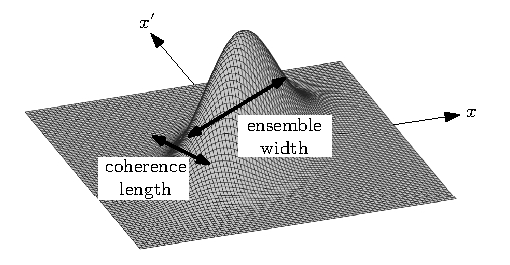
\includegraphics[width=.7\linewidth]{figures/ch03_fig04.pdf}
\caption{Gaussian密度行列(3.79)の記述に関係する、主な量のいくつかの図解。密度行列の非対角方向$x=-x'$における広がりは、系が空間的干渉効果を示しうる特徴的距離を測るコヒーレンス長$\ell(t)\equiv1/\sqrt{8A(t)}$で定量化される。アンサンブル幅$\Delta X(t)\equiv1/\sqrt{8C(t)}$は、異なる位置$x$についての確率分布$P(x,t)\equiv\rho_{\mathrm S}(x,x,t)$の大きさを表す。}\label{fig:3.4}
\end{figure}

% 原文 p.141
\hypertarget{srcpage:141}{}\label{srcpage:141}
他方、$\rho_{\mathrm S}(x,x',t)$の対角方向$x=x'$での幅は、確率分布$P(x,t)\equiv\rho_{\mathrm S}(x,x,t)$の大きさに対応する。この分布は、位置測定で系が$x$に見いだされる確率を記述する。この幅は$\sqrt{C(t)}$に反比例する［(3.79)参照］。したがって、位置空間アンサンブルの全体の大きさを定量化するアンサンブル幅$\Delta X(t)$を
\begin{equation}
\Delta X(t)=\frac{1}{\sqrt{8C(t)}}
\tag{3.81}
\end{equation}
と導入する。

係数$B(t)$は、$A(t)$および$C(t)$とともに、運動量分布の幅$\Delta P(t)$に関係し、これは
\begin{equation}
\Delta P(t)=\sqrt2\left[A(t)+\frac{B^2(t)}{4C(t)}\right]^{1/2}
\tag{3.82}
\end{equation}
で与えられる。(3.81)、(3.82)を用いると、対応する不確定性関係は
\begin{equation}
\Delta X(t)\Delta P(t)=\frac12\left[\frac{A(t)}{C(t)}+\frac{B^2(t)}{4C(t)}\right]^{1/2}
\tag{3.83}
\end{equation}
と書ける。最後に、項$D(t)$は、密度行列のトレースが常に保存されることを保証する。

Gaussian型の仮定(3.79)を運動方程式(3.78)に代入すると、係数$A(t)$、$B(t)$、$C(t)$、$D(t)$についての連立微分方程式が得られ、任意の初期条件に対して具体的に解ける（例えば文献\cite{ref017}の付録A2を参照）。ここでは、特定の初期状態、すなわち$x=0$を中心とする幅$b$の純粋状態のGaussian波束
\begin{equation}
\psi(x,0)=\left[\frac{1}{2\pi b^2}\right]^{1/4}\exp\left(\frac{-x^2}{4b^2}\right)
\tag{3.84}
\end{equation}
を選び、縮約密度行列のデコヒーレンスの動力学を示そう。これから初期密度行列
\begin{equation}
\rho_{\mathrm S}(x,x',0)=\left[\frac{1}{2\pi b^2}\right]^{1/2}\exp\left(-\frac{x^2+x'^2}{4b^2}\right)
\tag{3.85}
\end{equation}
を得る。これは(3.79)に現れる係数について、初期値$A(0)=C(0)=1/8b^2$、$B(0)=D(0)=0$に対応する。

密度行列(3.85)を図3.5に示す。Gaussianは$x$軸と$x'$軸に関して対称であり、すなわちコヒーレンス長とアンサンブル幅の大きさが等しい。この初期状態(3.85)に対して、係数$A(t)$、$B(t)$、$C(t)$、$D(t)$の時間依存性は容易に計算できる。$A(t)$、$C(t)$の表式を具体的に書けば（導出は文献\cite{ref007}、または文献\cite{ref017}の付録A2を参照）、
\begin{equation}
A(t)=\frac{\Lambda t^3+3m^2b^2/2+2\Lambda^2b^2t^4+12\Lambda m^2b^4t}{3t^2+8\Lambda b^2t^3+12m^2b^4}
\tag{3.86}
\end{equation}
および
\begin{equation}
C(t)=\frac12\left[\frac{t^2}{m^2b^2}+\frac83\frac{\Lambda t^3}{m^3}+4b^2\right]^{-1}
\tag{3.87}
\end{equation}
となる。
\begin{figure}[htbp]\centering
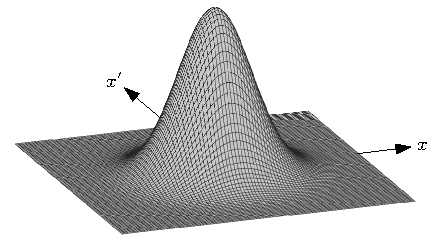
\includegraphics[width=.7\linewidth]{figures/ch03_fig05.pdf}
\caption{初期密度行列$\rho_{\mathrm S}(x,x',0)$［(3.85)参照］の図解。密度行列は$(x,x')$平面で対称なGaussianの形をもち、コヒーレンス長$\ell(0)$（「非対角」$x=-x'$に沿う広がり）が、アンサンブル幅$\Delta X(0)$（対角$x=x'$に沿う幅）に等しい。}\label{fig:3.5}
\end{figure}

% 原文 p.142
\hypertarget{srcpage:142}{}\label{srcpage:142}
コヒーレンス長、アンサンブル幅、縮約密度行列の純度などの主要な関連量の時間発展を調べる前に、環境散乱によるデコヒーレンスを考慮したとき、初期Gaussian(3.85)が時間とともにどのように発展すると予想されるかを、簡単に論じよう。環境との相互作用によって、与えられた距離$\Delta x=|x-x'|$にわたる空間的コヒーレンスの観測が、ますます難しくなると予想される。すなわち、コヒーレンス長$\ell(t)$［(3.80)参照］は時間とともに減少し、「古典的」対角線$x=x'$に垂直な方向にGaussian(3.85)を「絞る」と期待される。完全なデコヒーレンスの極限では、Gaussianは、対角線$x=x'$に沿う無限に細い稜線という、準古典的分布の形に近づくだろう。同時に、$x=-x'$方向の絞り込みに伴って、$x=x'$方向には広がると予想される。

係数$A(t)$、$C(t)$の具体的な表式(3.86)、(3.87)を用い、関連する量の時間発展を調べて、これらの直観を確認しよう。デコヒーレンスについて最も関心がある量は、おそらく(3.80)で定義したコヒーレンス長$\ell(t)$である。(3.86)を用いると、その時間依存性は
\begin{equation}
\ell(t)=\frac{1}{\sqrt{8A(t)}}=\frac12\left[\frac{3t^2+8\Lambda b^2t^3+12m^2b^4}{2\Lambda t^3+3m^2b^2+4\Lambda^2b^2t^4+24\Lambda m^2b^4t}\right]^{1/2}
\tag{3.88}
\end{equation}
で与えられる。

% 原文 p.143
\hypertarget{srcpage:143}{}\label{srcpage:143}
予想どおり、$t=0$でコヒーレンス長は波束の幅$b$に等しい。環境との相互作用がない場合（$\Lambda=0$）、$\ell(t)$は
\begin{equation}
\ell_{\mathrm{free}}(t)=\frac12\left[\frac{t^2}{m^2b^2}+4b^2\right]^{1/2}=\Delta X_{\mathrm{free}}(t)
\tag{3.89}
\end{equation}
となる。この表式は、本章の初めで論じた波束の自由なコヒーレント拡散を記述するにすぎない。これは、$\sigma\equiv\sqrt2b$と明らかに同定すれば、(3.3)に相当する（本節では$\hbar\equiv1$と置いたことも思い出そう）。

$\ell(t)$［(3.88)参照］の時間発展を詳しく調べよう。以下では、時間を$\tau_b\equiv1/\Lambda b^2$の単位で測る。これは、距離$\Delta x=b$（波束の初期幅）にわたる空間的コヒーレンスの特徴的な局在化時間尺度である。$\ell(t)$のグラフを図3.6に示す。

まず、局在化時間尺度$\tau_b$よりはるかに短い時刻$t$での$\ell(t)$の時間発展を調べよう。(3.88)を$\Lambda b^2t=0$のまわりで$\Lambda b^2t$の1次まで展開すると
\begin{equation}
\ell(t)\approx b(1-4\Lambda b^2t)
\tag{3.90}
\end{equation}
を得る。したがって、環境散乱の影響により、短時間ではコヒーレンス長は時間に対して線形に減少し、その減少率は散乱定数$\Lambda$に比例することがわかる。
\begin{figure}[htbp]\centering
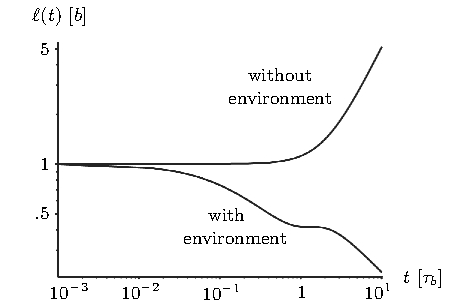
\includegraphics[width=.7\linewidth]{figures/ch03_fig06.pdf}
\caption{Joosら\cite{ref017}が調べたGaussian波束について、(3.88)で与えられるコヒーレンス長$\ell(t)$の時間依存性。時間$t$は特徴的な局在化時間尺度$\tau_b=1/\Lambda b^2$を単位として測り、$\ell(t)$は波束の初期幅$\ell(0)=b$を単位として表示した。上の曲線は環境との相互作用がない場合（$\Lambda=0$）の振る舞いを示す。下の曲線は環境散乱の効果を示し、系が空間的コヒーレンスを維持できる距離が時間とともに急速に減少することを示している。}\label{fig:3.6}
\end{figure}

% 原文 p.144
\hypertarget{srcpage:144}{}\label{srcpage:144}
一方、$t$が局在化時間尺度$\tau_b$よりはるかに長い極限も考えられる。巨視的物体の散乱率$\Lambda$が非常に大きな値を取りうること（表3.1参照）を考えれば、この極限が適用されるために$t$自体が大きい必要はない。例えば、大きさ$a=10^{-3}\,\mathrm{cm}$の塵粒子に対し、$\Lambda\approx10^{20}\,\mathrm{cm}^{-2}\,\mathrm s^{-1}$というかなり低い値を用い、初期のコヒーレントな広がりを大きさの10\%、すなわち$b=10^{-4}\,\mathrm{cm}$としても、$\tau_b\approx10^{-12}\,\mathrm s$を得る。したがって、巨視的物体では、通常、1秒に満たないごく短い時間で$t\gg\tau_b$の極限に達する。この極限では、(3.88)は漸近表式
\begin{equation}
\ell(t)\longrightarrow\frac{1}{\sqrt{2\Lambda t}}
\tag{3.91}
\end{equation}
に近づく。したがって、この場合のコヒーレンス長は$t^{-1/2}$に従い、初期状態(3.84)の幅$b$には依存しない。

次に、アンサンブル全体の大きさ$\Delta X(t)$の時間発展を考えよう。(3.81)、(3.87)から
\begin{equation}
\Delta X(t)=\frac{1}{\sqrt{8C(t)}}=\frac12\left[\frac{t^2}{m^2b^2}+\frac83\frac{\Lambda t^3}{m^3}+4b^2\right]^{1/2}
\tag{3.92}
\end{equation}
を得る。環境との相互作用がない場合（$\Lambda=0$）、すなわち初期波動関数(3.84)で記述される自由粒子の純粋にユニタリーな時間発展では、$\Delta X(t)$は$\Lambda=0$で評価したコヒーレンス長$\ell(t)$の表式［(3.89)参照］と一致し、
\begin{equation}
\Delta X_{\mathrm{free}}(t)=\frac12\left[\frac{t^2}{m^2b^2}+4b^2\right]^{1/2}
\tag{3.93}
\end{equation}
となる。したがって、環境がなければ、広がりは、位置のアンサンブルを記述する$x=x'$方向と、空間的コヒーレンスを表す$x=-x'$方向で、まったく同じ速さで進む。これは、もちろん自由粒子に予想される振る舞いである。環境が存在しなければ、一方の方向を他方に対して特別扱いする物理的機構は存在しない。しかし、環境を含めると非対称性が導入される。散乱事象は、系の位置を測る一種の測定装置として働くようになる。大まかにいえば、散乱粒子は、二つの位置の和$(x+x')$には鈍感なまま、二つの位置$x$、$x'$の差$|x-x'|$を識別しようとする。座標$(x+x')$と$(x-x')$に関する環境監視過程のこの非対称性は、$\rho_{\mathrm S}(x,x',t)$の運動方程式の形［(3.78)の右辺参照］にまとめられており、(3.92)と(3.88)の比較からわかるように、$\Delta X(t)$と$\ell(t)$の異なる時間発展をもたらす。

% 原文 p.145
\hypertarget{srcpage:145}{}\label{srcpage:145}
環境相互作用が存在すると、(3.92)の余分な項$\frac83\frac{\Lambda t^3}{m^3}$により、アンサンブルの幅は時間とともにいっそう速く増大する（図3.7参照）。\footnote{一見すると、驚くべき結果に思えるかもしれない。本章の導入では、デコヒーレンスは波束の拡散に対抗すると述べたのだから。しかし、ここには矛盾はない。肝心なのは、コヒーレントな拡散とアンサンブルの拡散の違いを念頭に置くことである。コヒーレントな拡散とは、例えば干渉実験を行うことによって、系が、ますます大きく離れた位置の重ね合わせにあるとわかることを意味する。これに対し、アンサンブルの拡散は、位置測定で系を見いだしうる位置の範囲が増大することに対応するだけである。}この模型で、環境の存在がこの「古典的」拡散を加速するのは、散乱事象によって系の平均エネルギーが増加するためである。このエネルギー増加は、散乱事象によって系に反跳が生じないという仮定の帰結である（121ページ参照）。

こうして、密度行列の時間発展は、図3.8に示すように、二つの逆向きの影響の競合として視覚化できる。一方では、自由粒子のユニタリーな発展と、散乱事象による平均エネルギーの増加の両方によって、位置空間アンサンブル全体の空間的広がり$\Delta X(t)$が、時間とともにますます広がる。他方、同じ散乱事象は系の位置の連続的監視としても働き、コヒーレンス長$\ell(t)$を減少させ、したがって次第に短い距離にわたる空間的コヒーレンスまで抑制する。
\begin{figure}[htbp]\centering
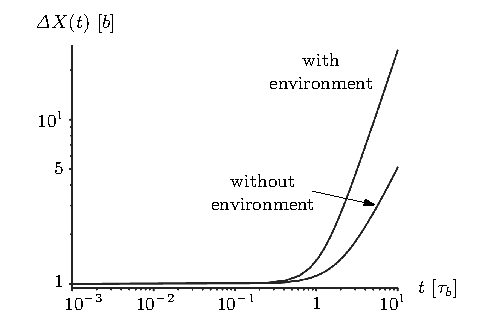
\includegraphics[width=.7\linewidth]{figures/ch03_fig07.pdf}
\caption{Joosら\cite{ref017}が調べたGaussian波束について、(3.92)で与えられるアンサンブル幅$\Delta X(t)$の時間発展。時間$t$は特徴的な局在化時間尺度$\tau_b=1/\Lambda b^2$を単位として測り、$\Delta X(t)$は波束の初期幅$\Delta X(0)=b$を単位として示した。}\label{fig:3.7}
\end{figure}
% 原文 p.146
\hypertarget{srcpage:146}{}\label{srcpage:146}
\begin{figure}[htbp]\centering
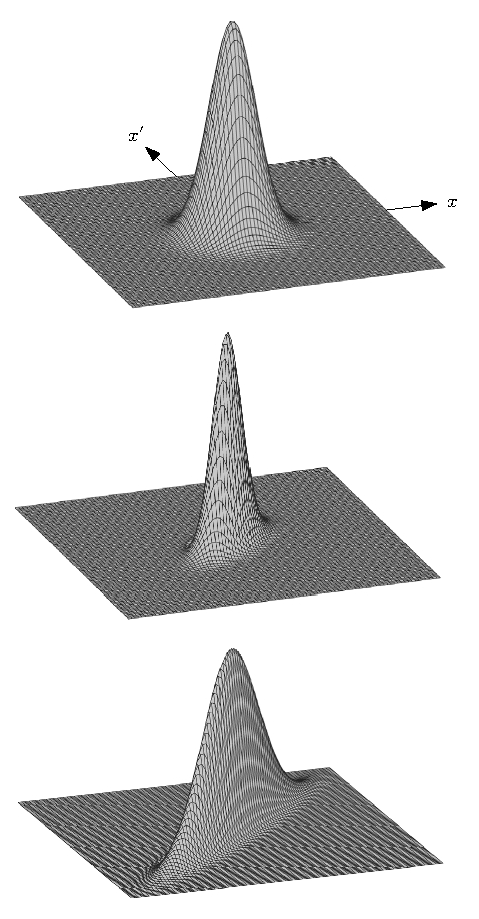
\includegraphics[width=.63\linewidth]{figures/ch03_fig08.pdf}
\caption{散乱環境の影響下における、(3.85)の初期状態をもつGaussian波束(3.79)の時間発展。(3.79)の係数$A(t)$、$C(t)$は、それぞれ(3.86)、(3.87)によって定まる。空間的コヒーレンスを表す非対角方向$x=-x'$におけるGaussianの幅は次第に縮まり、密度行列は対角線$x=x'$に集中した準古典的な位置の確率分布に近づく。}\label{fig:3.8}
\end{figure}

% 原文 p.147
\hypertarget{srcpage:147}{}\label{srcpage:147}
コヒーレンス長$\ell(t)$の減少と、アンサンブルの大きさ$\Delta X(t)$の増大の相互作用を定量化するため、両者を組み合わせた無次元量として、しばしば比
\begin{equation}
\delta(t)\equiv\frac{\ell(t)}{\Delta X(t)}=\sqrt{\frac{C(t)}{A(t)}}
\tag{3.94}
\end{equation}
を考える（例えば文献\cite{ref017,ref173}）。$\delta(t)$のグラフを図3.9に示す。環境がなければ$\delta(t)$は一定である。すなわち、コヒーレントな拡散は$x=x'$方向と$x=-x'$方向で同じ速さで進む［(3.89)とそれに続く議論を参照］。環境を含めると、コヒーレンス長$\ell(t)$は減少する一方、全体の幅$\Delta X(t)$は増大する。しかし、$\Delta X(t)$の増大率は$\ell(t)$の減少率より遅く、結果として$\delta(t)$は減少する。

量$\delta(t)$を導入したもう一つの理由は、別のデコヒーレンスの尺度、すなわち2.4.3節で導入した密度行列$\hat\rho$の純度$\varsigma=\operatorname{Tr}(\hat\rho^2)$［(2.30)参照］と、容易に直接結びつけられることである。この模型の縮約密度行列$\rho_{\mathrm S}(t)$の純度は
\begin{equation}
\varsigma(t)=\sqrt{\frac{C(t)}{A(t)}}
\tag{3.95}
\end{equation}
となる。しかし、これは明らかに$\delta(t)$の表式(3.94)と一致する。すなわち、量$\delta(t)$は、散乱模型の縮約密度行列の純度も記述する。図3.9から、予想どおり環境散乱は縮約密度行列の純度を減少させ、デコヒーレンスの漸進的な作用を反映することがわかる。
\begin{figure}[htbp]\centering
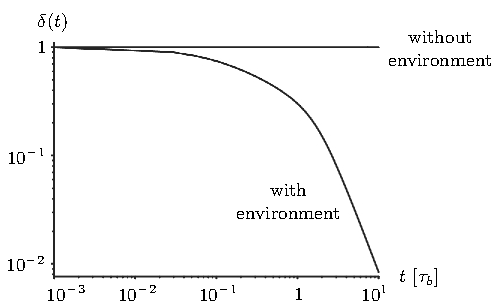
\includegraphics[width=.7\linewidth]{figures/ch03_fig09.pdf}
\caption{環境散乱がある場合とない場合の比$\delta(t)\equiv\ell(t)/\Delta X(t)$［(3.94)参照］の時間依存性。量$\delta(t)$は、この模型の局所密度行列の純度の時間発展も記述する。ここでも時間$t$は、特徴的な局在化時間尺度$\tau_b=1/\Lambda b^2$を単位として測る。}\label{fig:3.9}
\end{figure}

% 原文 p.148
\hypertarget{srcpage:148}{}\label{srcpage:148}
最後に、それぞれ$x=\pm x_0$を中心とする、(3.84)の形の二つのGaussian波束の、等しい重みをもつ重ね合わせ
\begin{equation}
\begin{aligned}
\Psi(x,0)&=\psi_{x_0}(x,0)+\psi_{-x_0}(x,0)\\
&=\left[\frac{1}{2\pi b^2}\right]^{1/4}\left\{\exp\left(\frac{-(x-x_0)^2}{4b^2}\right)+\exp\left(\frac{-(x+x_0)^2}{4b^2}\right)\right\}
\end{aligned}\tag{3.96}
\end{equation}
の時間発展を示そう。この波動関数を図3.10に示す。

$x_0\gg b$であれば、このような量子状態は、距離$2x_0$離れた明確で区別可能な二つの位置の重ね合わせによって粒子が記述される、非古典的な状況に対応する。対応する密度行列は
\begin{equation}
\begin{aligned}
\rho_{\mathrm S}(x,x',0)&=\Psi^*(x',0)\Psi(x,0)\\
&=\psi_{x_0}^*(x',0)\psi_{x_0}(x,0)+\psi_{-x_0}^*(x',0)\psi_{-x_0}(x,0)\\
&\quad+\psi_{x_0}^*(x',0)\psi_{-x_0}(x,0)+\psi_{-x_0}^*(x',0)\psi_{x_0}(x,0)
\end{aligned}\tag{3.97}
\end{equation}
である。この密度行列を、図3.11の最上段に示す。非対角線$x=-x'$に沿う二つのピークは、(3.96)で導入した二つの波束$\psi_{x_0}(x,0)$、$\psi_{-x_0}(x,0)$の間の空間的干渉項$\psi_{x_0}^*(x',0)\psi_{-x_0}(x,0)$、$\psi_{-x_0}^*(x',0)\psi_{x_0}(x,0)$に対応する。

運動方程式(3.78)で決まる、密度行列(3.97)のその後の時間発展を、図3.11に示す。予想どおり、$x=\pm x_0$のまわりの二つの領域の間の空間的コヒーレンスに対応する干渉項は、環境の存在によって次第に抑制される。完全なデコヒーレンスの極限では、それぞれ$+x_0$、$-x_0$のまわりへの系の局在化を記述する、二つの状態の（ただし非真正な！）アンサンブルを得る。すなわち、系だけに関係する測定では、このアンサンブルを、対応する局在した位置の古典的な（真正な）アンサンブルと区別できない。
\begin{figure}[htbp]\centering
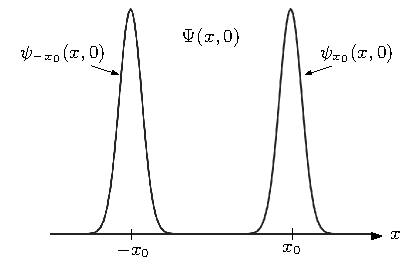
\includegraphics[width=.65\linewidth]{figures/ch03_fig10.pdf}
\caption{それぞれ$+x_0$、$-x_0$を中心とする、二つのGaussian波束の重ね合わせ(3.96)の図解。}\label{fig:3.10}
\end{figure}
% 原文 p.149
\hypertarget{srcpage:149}{}\label{srcpage:149}
\begin{figure}[htbp]\centering
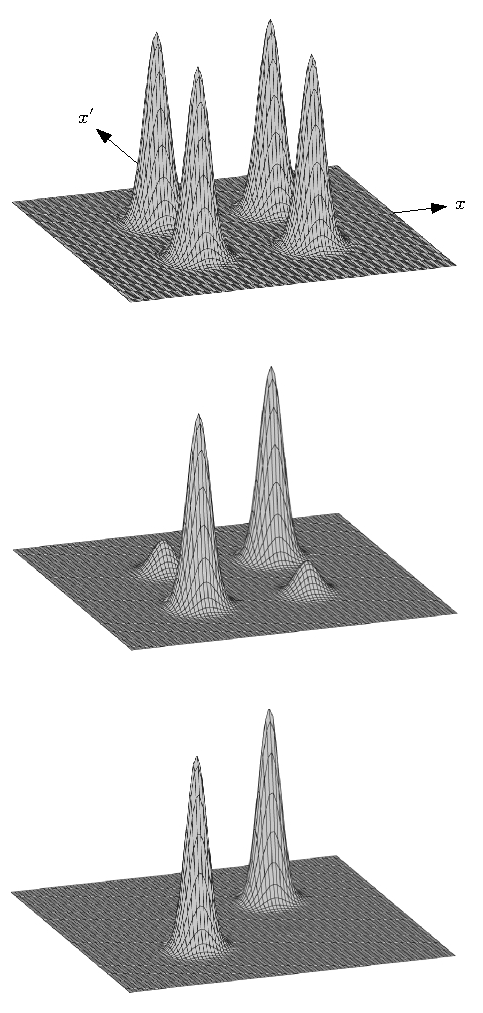
\includegraphics[width=.63\linewidth]{figures/ch03_fig11.pdf}
\caption{二つのGaussian波束の重ね合わせ(3.96)についての、密度行列$\rho_{\mathrm S}(x,x',t)$の時間発展。非対角線$x=-x'$に沿う干渉項が、環境粒子の散乱によって次第に減衰する。}\label{fig:3.11}
\end{figure}

% 原文 p.150
\hypertarget{srcpage:150}{}\label{srcpage:150}
\subsectionlink{まとめ}
環境粒子の散乱は、巨視的領域における主要なデコヒーレンス源の一つであり、したがって、身の回りの日常世界に古典性が出現するうえで、きわめて重要な役割を果たす。散乱によるデコヒーレンスは、例えば、環境が系の位置の連続的監視装置として働くことの帰結としてデコヒーレンスを理解するという、基本的な概念面を説明するのにも、まさに適している。

一回の散乱事象が不完全な経路情報しか環境に符号化しない場合（「長波長極限」）、空間的干渉項は［(3.57)参照］
\begin{equation}
\rho_{\mathrm S}(\bm x,\bm x',t)=\rho_{\mathrm S}(\bm x,\bm x',0)e^{-\Lambda(\bm x-\bm x')^2t}
\tag{3.98}
\end{equation}
に従って指数関数的に減衰することがわかった。散乱定数$\Lambda$は、散乱過程の具体的な物理的性質を担っている。したがって、距離$\Delta x=|\bm x-\bm x'|$にわたる空間的干渉のデコヒーレンスの特徴的時間尺度$\tau_{\Delta x}$は［(3.58)参照］
\begin{equation}
\tau_{\Delta x}=\frac{1}{\Lambda(\Delta x)^2}
\tag{3.99}
\end{equation}
である。$\tau_{\Delta x}$は、コヒーレントな隔たり$\Delta x$に対して二次的に減少する。この隔たりが環境粒子の典型的な波長より大きくなると、一回の散乱事象で完全に識別されるようになる。それに伴って、デコヒーレンス率は飽和し、全散乱率だけで与えられる［(3.48)参照］。

また、典型的なデコヒーレンス時間尺度の具体的な数値もいくつか見積もり、散乱によるデコヒーレンスの有効性と遍在性を印象的に示した。一見すると、系を環境から適切に遮蔽すれば、デコヒーレンスを完全に避けられると思ったかもしれない。しかし、見てきたように、実際には、そのような完全な遮蔽を達成することは不可能である。利用できる最良の実験室真空でさえ、空気分子の密度は、巨視的な空間的干渉を強く、事実上瞬時に減衰させるほど大きい。仮に周囲の気体分子が系と相互作用することを完全に防げたとしても、熱光子が急速なデコヒーレンスを引き続き生じさせるだろう。さらにその効果を小さくできても、逃れられない太陽ニュートリノとマイクロ波背景放射の環境によるデコヒーレンスは、なお生じる。これらの議論は、巨視的尺度において位置が遍在的な優先基底となる理由（また、2.8.4節で述べたキラル分子など、しばしば微視的尺度でもそうなる理由）も示している。

% 原文 p.151
\hypertarget{srcpage:151}{}\label{srcpage:151}
量子系を散乱環境の影響から遮蔽することは実際には不可能であり、こうした散乱過程が系の運動と観測可能な量子特性に決定的な影響を与えるという認識は、波束を、身の回りにある空間的に広がった物体と直接同一視する真の「波動力学」を目指したSchrödingerの試みに、欠けていた重要な要素を与えた。散乱環境に接している物体を記述する縮約密度行列を用いれば、次第に減少するコヒーレンス長によって幅が与えられる波束の、非真正なアンサンブルを定義できる。そのような個々の波束を、少なくとも局所測定という操作的な意味では、よく局在した粒子の現れと同一視できる。

6.2節で詳しく論じるように、大きな分子を用いた最近の二重スリット型実験によって、散乱によるデコヒーレンス模型の定性的・定量的な予測を、直接確認できるようになった。この種の実験が、いっそう大きな物体に干渉縞を生成し、デコヒーレンスの漸進的な影響を観測する方向へ進むにつれて、実験室で、ますます巨視的な尺度において、これらの模型を直接検証できるようになるだろう。

\clearpage
\setcounter{section}{3}
\setcounter{footnote}{0}
% 原文 printed pp.153--170 / PDF pp.167--184
\sectionlink{デコヒーレンスのマスター方程式による定式化}
% 原文 p.153
\hypertarget{srcpage:153}{}\label{srcpage:153}
本章では、いわゆるマスター方程式を用いる、デコヒーレンスの動力学の記述を導入する。このようなマスター方程式は、環境Eと相互作用する開いた量子系Sの縮約密度行列$\hat\rho_{\mathrm S}(t)$の時間発展を、直接、便利な形で与える。これを用いれば、まず系と環境の全体の運動を求め、その後、環境の自由度についてトレースを取る必要がなくなる。マスター方程式の方法を動機づけるのは、二つの事情である。第一に、通常、環境や、系と環境の全体の運動には関心がなく、本当に知りたいのは、対象となる系に環境が及ぼす影響だけである。第二に、密度行列の時間発展を解析的に決定することは、しばしば不可能である。そのような場合、近似法を用いて、縮約密度行列の近似的な発展のマスター方程式を得ることができる。

閉じた系の密度行列の運動とは異なり、縮約密度行列の発展方程式は、もちろん一般に非ユニタリーである。環境との相互作用は、通常、系に存在するコヒーレンスの量を変えるからである。より形式的にいえば、縮約密度行列を得るためのトレース操作は非ユニタリーな操作なので、一般にマスター方程式も非ユニタリーでなければならない。

本章の構成は次のとおりである。4.1節ではマスター方程式の基本的な考え方と一般的形式を導入する。4.2節では、非常に重要な種類のマスター方程式、いわゆるBorn--Markovマスター方程式を、やや詳しく論じる。このマスター方程式は、デコヒーレンスの研究で重要な役割を果たす。4.2.2節で与えるこの方程式の導出は、どうしても多少技術的になるので、そこをざっと眺めるだけにするか、完全に飛ばす読者もいるかもしれない。4.3節では、追加の仮定のもとで成り立つ、一般のBorn--Markovマスター方程式の特別で、より単純な形である、いわゆるLindbladマスター方程式を論じる。後で見るように、Lindbladマスター方程式は、デコヒーレンス過程の非常に直観的な表示を可能にする。最後に4.4節では、非Markov的な運動の場合を簡単に論じる。

マスター方程式は、いわゆる量子力学的半群の理論でも重要な役割を果たす。ただし、ここではデコヒーレンスの模型化に焦点を当てるため、マスター方程式と力学的半群の数学的関係は、これ以上論じない。この主題について関心のある読者には、詳しい情報として文献\cite{ref017}の第7章と、BreuerとPetruccioneの著書\cite{ref018}を参照していただきたい。

% 原文 p.154
\hypertarget{srcpage:154}{}\label{srcpage:154}
\subsectionlink{一般的形式}
デコヒーレンスの「通常の」形式では、縮約密度行列$\hat\rho_{\mathrm S}(t)$は
\begin{equation}
\hat\rho_{\mathrm S}(t)=\operatorname{Tr}_{\mathrm E}\{\hat\rho_{\mathrm{SE}}(t)\}
\equiv\operatorname{Tr}_{\mathrm E}\{\hat U(t)\hat\rho_{\mathrm{SE}}(0)\hat U^{\dagger}(t)\}
\tag{4.1}
\end{equation}
によって計算する。$\hat U(t)$は、複合系SEの時間発展演算子である。(4.1)から明らかなように、この方法では、トレース操作によって縮約された記述に到達する前に、必ず全系SEの運動$\hat\rho_{\mathrm{SE}}(t)$を決定しなければならない。本章の導入で述べたように、ある程度複雑な模型系の大部分では、この作業を実際に行うことは、不可能とまではいわなくとも非常に難しい。

これに対し、マスター方程式の形式では、代わりに
\begin{equation}
\hat\rho_{\mathrm S}(t)=\hat V(t)\hat\rho_{\mathrm S}(0)
\tag{4.2}
\end{equation}
という形の表式から、$\hat\rho_{\mathrm S}(t)$を直接計算する。演算子$\hat V(t)$は、$\hat\rho_{\mathrm S}(t)$の発展を生成する、いわゆる力学的写像である。$\hat V(t)$は、別の演算子に作用する演算子を表すため、通常「超演算子」と呼ばれる。(4.2)は$\hat\rho_{\mathrm S}(t)$のマスター方程式と呼ばれ、このようなマスター方程式が取りうる最も一般的な形を表す。

明らかに、マスター方程式が厳密であれば、定義上(4.1)と(4.2)は同値でなければならない。すなわち恒等式
\begin{equation}
\hat V(t)\hat\rho_{\mathrm S}(0)\equiv\operatorname{Tr}_{\mathrm E}\{\hat U(t)\hat\rho_{\mathrm{SE}}(0)\hat U^{\dagger}(t)\}
\tag{4.3}
\end{equation}
が成り立たなければならず、その場合、マスター方程式は(4.1)の自明な書き換えにすぎない。

したがって、マスター方程式の力が発揮されるのは、系と環境の状態と運動について、何らかの仮定を課して初めてである。そのような仮定により、全体の厳密な運動$\hat\rho_{\mathrm{SE}}(t)$を計算できないときでも、$\hat\rho_{\mathrm S}(t)$の近似的な時間発展を決定できる。実際、ここでは、ある近似から得られる、時間について局所的な1階微分方程式として書けるマスター方程式に、注意を限定する。すなわち
\begin{equation}
\frac{\mathrm d}{\mathrm dt}\hat\rho_{\mathrm S}(t)=\hat L[\hat\rho_{\mathrm S}(t)]
=\underbrace{-\mathrm i[\hat H'_{\mathrm S},\hat\rho_{\mathrm S}(t)]}_{\text{ユニタリーな発展}}
+\underbrace{\hat D[\hat\rho_{\mathrm S}(t)]}_{\text{デコヒーレンス}}
\tag{4.4}
\end{equation}
という形のものである。

% 原文 p.155
\hypertarget{srcpage:155}{}\label{srcpage:155}
この方程式は、時刻$t$での$\hat\rho_{\mathrm S}$の変化が、同じ$t$で評価した$\hat\rho_{\mathrm S}$のみに依存し、他の時刻$t'\ne t$には依存しないという意味で、時間について局所的である。(4.4)に現れる超演算子$\hat L$は$\hat\rho_{\mathrm S}(t)$に作用し、通常、環境の初期状態とHamiltonianの各項に依存する。この超演算子の背後にある物理的直観を伝えるため、$\hat L$を二つの部分に分解した。
\begin{enumerate}
\item Hamiltonian $\hat H'_{\mathrm S}$との、通常のLiouville--von Neumann交換子で与えられるユニタリーな部分。このHamiltonianは、環境がなければSの発展を生成する、Sの摂動のない自由Hamiltonian $\hat H_{\mathrm S}$とは、一般に同一ではないことに注意する必要がある。環境の存在は、しばしば自由Hamiltonianを摂動し、系のエネルギー準位の繰り込みをもたらすからである。この効果（しばしばLambシフトの寄与と呼ばれる）は、環境によって生じる非ユニタリーな発展とは無関係で、縮約された運動のユニタリーな部分だけを変えることを強調しておく。
\item 環境によるデコヒーレンス（場合によっては散逸も）を表す、非ユニタリーな部分$\hat D[\hat\rho_{\mathrm S}(t)]$。以下では、この項が主な関心の対象となる。
\end{enumerate}
系の発展が完全にユニタリーなら、$\hat D[\hat\rho_{\mathrm S}(t)]=0$であり、(4.4)は単に
\begin{equation}
\frac{\mathrm d}{\mathrm dt}\hat\rho_{\mathrm S}(t)=-\mathrm i[\hat H'_{\mathrm S},\hat\rho_{\mathrm S}(t)]
\tag{4.5}
\end{equation}
となる。この方程式と、閉じた系に対する標準のLiouville--von Neumann方程式との唯一の違いは、摂動のないHamiltonian $\hat H_{\mathrm S}$の代わりに、環境によってシフトした系のHamiltonian $\hat H'_{\mathrm S}$を用いる点である。

次節では、ある一組の仮定のもとで、$\hat L$、すなわち$\hat H'_{\mathrm S}$と$\hat D[\hat\rho_{\mathrm S}(t)]$の、具体的で一般的な表式を導く。得られたマスター方程式を与えられた模型に適用すれば、すべての時刻$t$における$\hat\rho_{\mathrm S}(t)$の時間発展を計算できる。

\subsectionlink{Born--Markovマスター方程式}
Born--Markovマスター方程式は、開いた量子系とデコヒーレンスの研究において、きわめて重要な役割を果たす。これにより、多くのデコヒーレンスの問題を、数学的に簡単な、しばしば閉じた形で扱える。この方程式に基づく模型の予測と実験データの比較から、マスター方程式の基礎にあるBornとMarkovの仮定は、多くの場合に妥当であることが示されている。しかし、Markov的な運動に従わず、したがってBorn--Markovマスター方程式では適切に模型化できないことの多い重要な物理系（例えば低温の固体系）も、いろいろと存在することを、この段階で強調しておく必要がある。この点には、後の4.4節で戻る。

% 原文 p.156
\hypertarget{srcpage:156}{}\label{srcpage:156}
\subsubsectionlink{Born--Markovマスター方程式の構造}
Born--Markovマスター方程式は、大まかには次のように述べられる、二つの中心的な近似に基づいている（これらの近似の形式的表現と物理的正当化については、後の4.2.2節で詳しく論じる）。
\begin{enumerate}
\item \textbf{Born近似。}系と環境の結合は十分弱く、環境は十分大きいため、環境の密度演算子の変化は無視でき、系と環境の状態は、常に近似的な積状態にとどまる。すなわち
\begin{equation}
\hat\rho(t)\approx\hat\rho_{\mathrm S}(t)\otimes\hat\rho_{\mathrm E},
\tag{4.6}
\end{equation}
であり、$\hat\rho_{\mathrm E}$は常にほぼ一定である。
\item \textbf{Markov近似。}系との結合で作られる環境内部の自己相関は、系の状態が顕著に変化する特徴的時間尺度に比べて速く減衰するという意味で、環境の「記憶効果」は無視できる。
\end{enumerate}
これらの仮定が成り立つとしよう。さらに、系Sは自己Hamiltonian $\hat H_{\mathrm S}$をもち、環境との結合は、対角形
\begin{equation}
\hat H_{\mathrm{int}}=\sum_\alpha\hat S_\alpha\otimes\hat E_\alpha
\tag{4.7}
\end{equation}
に書ける相互作用Hamiltonian $\hat H_{\mathrm{int}}$によって記述されるとする［(2.93)参照］。系と環境の演算子$\hat S_\alpha$、$\hat E_\alpha$はユニタリーだが、必ずしもHermiteではない。2.8節で説明したように、対角分解(4.7)の直観的な物理解釈は、$\hat S_\alpha$が、環境によって連続的に「監視」される系の物理量に対応するというものである（ただし$\hat S_\alpha$がHermiteの場合）。

このとき、縮約密度演算子$\hat\rho_{\mathrm S}(t)$の発展は、Born--Markovマスター方程式
\begin{equation}
\frac{\mathrm d}{\mathrm dt}\hat\rho_{\mathrm S}(t)=-\mathrm i[\hat H_{\mathrm S},\hat\rho_{\mathrm S}(t)]
-\sum_\alpha\left\{[\hat S_\alpha,\hat B_\alpha\hat\rho_{\mathrm S}(t)]+[\hat\rho_{\mathrm S}(t)\hat C_\alpha,\hat S_\alpha]\right\}
\tag{4.8}
\end{equation}
で与えられる。この式に現れる系の演算子$\hat B_\alpha$、$\hat C_\alpha$の定義は
\begin{align}
\hat B_\alpha&\equiv\int_0^\infty\mathrm d\tau\sum_\beta C_{\alpha\beta}(\tau)\hat S_\beta^{(\mathrm I)}(-\tau),\tag{4.9a}\\
\hat C_\alpha&\equiv\int_0^\infty\mathrm d\tau\sum_\beta C_{\beta\alpha}(-\tau)\hat S_\beta^{(\mathrm I)}(-\tau)\tag{4.9b}
\end{align}
である。

% 原文 p.157
\hypertarget{srcpage:157}{}\label{srcpage:157}
ここで$\hat S_\alpha^{(\mathrm I)}(-\tau)$は、いわゆる相互作用描像の系演算子$\hat S_\alpha$を表す。相互作用描像は、以下のBorn--Markovマスター方程式の導出で多用するため、付録で復習する。以下では、表記を簡単にするため、相互作用描像の演算子を表す上付き添字「I」を省略する。代わりに、陽な時間引数をもつ演算子は、すべて相互作用描像の演算子と理解するという約束を導入する。ただし密度演算子では、やはり時間引数をもつSchrödinger描像の密度演算子（Schrödinger描像では量子状態が陽に時間に依存するため）との違いを明確にするため、上付き添字の表記を維持する。

(4.9)に現れる量$C_{\alpha\beta}(\tau)$は
\begin{equation}
C_{\alpha\beta}(\tau)\equiv\langle\hat E_\alpha(\tau)\hat E_\beta\rangle_{\hat\rho_{\mathrm E}}
\tag{4.10}
\end{equation}
で与えられ、平均は環境の初期状態$\hat\rho_{\mathrm E}$について取る［Born近似(4.6)では、$\hat\rho_{\mathrm E}$は常にほぼ一定にとどまることを思い出そう］。以下では、$C_{\alpha\beta}(\tau)$を環境自己相関関数と呼ぶ。この名称の理由は容易に理解できる。演算子$\hat E_\alpha$は、Hermiteであれば、系と環境の相互作用によって環境について「測定」される観測量とみなせる。環境自己相関関数は、特定の$\hat E_\alpha$のそのような「測定」の結果が、時間$\tau$後に行った同じ観測量の「測定」の結果と、どの程度相関しているかを教える。大まかにいえば、これらの関数は、系との相互作用についての情報を環境が時間とともにどの程度保持するかを定量化する。実際、Markov近似は、これらの環境自己相関関数が、系の発展によって定まる時間尺度と比べて速く減衰するという仮定に対応する。

Born--Markovマスター方程式の形(4.8)は、かなり威圧的で、具体例への適用が難しそうに見えるかもしれない。与えられた模型について、量$\hat B_\alpha$、$\hat C_\alpha$［(4.9)参照］を具体的に決めるには、(i)相互作用描像の演算子$\hat S_\alpha(\tau)$、$\hat E_\alpha(\tau)$（その時間発展は、それぞれ系と環境のHamiltonian $\hat H_{\mathrm S}$、$\hat H_{\mathrm E}$によって与えられる。付録参照）、(ii)環境自己相関関数$C_{\alpha\beta}(\tau)$［(4.10)参照］を計算しなければならない。

しかし、多くの関心ある状況では、マスター方程式(4.8)は大幅に簡単になる。例えば、大部分の場合、環境によって監視される系の観測量$\hat S$を一つだけ考えればよい。すると、相互作用Hamiltonianの対角分解(4.7)の和は一項だけになり、
\begin{equation}
\hat H_{\mathrm{int}}=\hat S\otimes\hat E
\tag{4.11}
\end{equation}
となる。
% 原文 p.158
\hypertarget{srcpage:158}{}\label{srcpage:158}
また、相互作用描像の演算子$\hat S_\alpha(\tau)$、$\hat E_\alpha(\tau)$の時間依存性もしばしば非常に簡単で、時には自明でさえあるため、量$\hat B_\alpha$、$\hat C_\alpha$［(4.9)参照］の計算が容易になる。これがどう働くかは、次の第5章で、Born--Markovマスター方程式(4.8)を具体例に適用する際に見る。
\subsubsectionlink{Born--Markovマスター方程式の導出}
本節では、Born--Markovマスター方程式(4.8)を第一原理から導く。とりわけ導出に入る仮定の理解を深めるため、読者には、主要な段階を実際に追っていただきたい。

\subsubsectionlink*{相互作用描像での記述}
まず、系と環境の全Hamiltonianを、通常の形
\begin{equation}
\hat H=\hat H_{\mathrm S}+\hat H_{\mathrm E}+\hat H_{\mathrm{int}}
\tag{4.12}
\end{equation}
に分解することから始めよう。摂動論を適用したいので、相互作用描像へ移るのが便利である。このとき
\begin{equation}
\hat H_0\equiv\hat H_{\mathrm S}+\hat H_{\mathrm E}
\tag{4.13}
\end{equation}
は全自由Hamiltonianであり、$\hat H_{\mathrm{int}}$は摂動的に扱う相互作用を表す。

相互作用Hamiltonian $\hat H_{\mathrm{int}}$と、系と環境の全密度演算子$\hat\rho(t)$を、相互作用描像へ変換する。この変換は［(A.4)、(A.5)参照］
\begin{align}
\hat H_{\mathrm{int}}(t)&=e^{\mathrm i\hat H_0t}\hat H_{\mathrm{int}}e^{-\mathrm i\hat H_0t},\tag{4.14}\\
\hat\rho^{(\mathrm I)}(t)&=e^{\mathrm i\hat H_0t}\hat\rho(t)e^{-\mathrm i\hat H_0t}
=e^{\mathrm i\hat H_0t}e^{-\mathrm i\hat Ht}\hat\rho e^{\mathrm i\hat Ht}e^{-\mathrm i\hat H_0t}\tag{4.15}
\end{align}
で与えられる。$\hat\rho^{(\mathrm I)}(t)$の時間発展は、相互作用描像でのLiouville--von Neumann方程式［(A.9)参照］
\begin{equation}
\frac{\mathrm d}{\mathrm dt}\hat\rho^{(\mathrm I)}(t)=-\mathrm i[\hat H_{\mathrm{int}}(t),\hat\rho^{(\mathrm I)}(t)]
\tag{4.16}
\end{equation}
で決まる。したがって、相互作用描像の密度演算子の発展は、全Hamiltonianのうち、相互作用描像での結合部分$\hat H_{\mathrm{int}}(t)$だけによって生成される。

% 原文 p.159
\hypertarget{srcpage:159}{}\label{srcpage:159}
\subsubsectionlink*{積分による反復解}
(4.16)を形式的に積分すると、
\begin{equation}
\hat\rho^{(\mathrm I)}(t)=\hat\rho(0)-\mathrm i\int_0^t\mathrm dt'\,[\hat H_{\mathrm{int}}(t'),\hat\rho^{(\mathrm I)}(t')]
\tag{4.17}
\end{equation}
を得る。この$\hat\rho^{(\mathrm I)}(t)$の表式を、(4.16)の右辺へ戻して代入しよう。すると
\begin{equation}
\begin{aligned}
\frac{\mathrm d}{\mathrm dt}\hat\rho^{(\mathrm I)}(t)
&=-\mathrm i\left[\hat H_{\mathrm{int}}(t),\hat\rho(0)-\mathrm i\int_0^t\mathrm dt'\,[\hat H_{\mathrm{int}}(t'),\hat\rho^{(\mathrm I)}(t')]\right]\\
&=-\mathrm i[\hat H_{\mathrm{int}}(t),\hat\rho(0)]
-\int_0^t\mathrm dt'\,[\hat H_{\mathrm{int}}(t),[\hat H_{\mathrm{int}}(t'),\hat\rho^{(\mathrm I)}(t')]]
\end{aligned}\tag{4.18}
\end{equation}
となる。さらに［導出は(A.12)参照］
\begin{equation}
\hat\rho^{(\mathrm I)}_{\mathrm S}(t)=\operatorname{Tr}_{\mathrm E}\{\hat\rho^{(\mathrm I)}(t)\}
\tag{4.19}
\end{equation}
なので、環境についてトレースを取るだけで、(4.18)を縮約密度演算子$\hat\rho^{(\mathrm I)}_{\mathrm S}(t)$の方程式に変換できる。
\begin{equation}
\begin{aligned}
\frac{\mathrm d}{\mathrm dt}\hat\rho^{(\mathrm I)}_{\mathrm S}(t)
&=-\mathrm i\operatorname{Tr}_{\mathrm E}[\hat H_{\mathrm{int}}(t),\hat\rho(0)]\\
&\quad-\int_0^t\mathrm dt'\,\operatorname{Tr}_{\mathrm E}[\hat H_{\mathrm{int}}(t),[\hat H_{\mathrm{int}}(t'),\hat\rho^{(\mathrm I)}(t')]].
\end{aligned}\tag{4.20}
\end{equation}
実際、一般性を失わずに
\begin{equation}
\operatorname{Tr}_{\mathrm E}[\hat H_{\mathrm{int}}(t),\hat\rho(0)]=0
\tag{4.21}
\end{equation}
と仮定できる。Hamiltonian $\hat H_0$、$\hat H_{\mathrm{int}}$を形式的に再定義すれば、常にこれを実現できることは容易に示せる。すると(4.20)は
\begin{equation}
\frac{\mathrm d}{\mathrm dt}\hat\rho^{(\mathrm I)}_{\mathrm S}(t)
=-\int_0^t\mathrm dt'\,\operatorname{Tr}_{\mathrm E}[\hat H_{\mathrm{int}}(t),[\hat H_{\mathrm{int}}(t'),\hat\rho^{(\mathrm I)}(t')]]
\tag{4.22}
\end{equation}
と簡単になる。

この式に至るまでの計算はすべて厳密であり、近似は一切行っていない。ここで少し立ち止まり、次の問いを考えよう。$\hat\rho^{(\mathrm I)}_{\mathrm S}(t)$のマスター方程式として望ましい性質のうち、(4.22)にはまだ何が欠けているだろうか。(4.22)の右辺は、依然として0から$t$までのすべての時刻で評価した、系と環境の全密度演算子$\hat\rho^{(\mathrm I)}$に依存している。したがって(4.22)は、まだ、$\hat\rho^{(\mathrm I)}_{\mathrm S}$の時刻$t$での変化を、$\hat\rho^{(\mathrm I)}_{\mathrm S}(t)$と一組の既知量だけで決める、(4.4)のような時間局所的な微分方程式ではない。そこで、二つの望ましい性質が浮かび上がる。

% 原文 p.160
\hypertarget{srcpage:160}{}\label{srcpage:160}
\begin{description}
\item[(P1)] マスター方程式を、縮約密度演算子$\hat\rho^{(\mathrm I)}_{\mathrm S}(t)$と環境の初期状態だけで完全に表したい。すなわち、時間に依存する環境状態に関係する項を除きたい。この性質を満たすマスター方程式は積分微分方程式と呼ばれる。ある時刻$t$での対象量の微分的変化が、すべての時刻$t'\leq t$にわたる、その量の関数の積分に依存するからである。
\item[(P2)] $\hat\rho^{(\mathrm I)}_{\mathrm S}$の時刻$t$での変化が、過去の時刻$t'<t$で評価した$\hat\rho^{(\mathrm I)}_{\mathrm S}$に依存しないようにしたい。
\end{description}
これらの目標を実現する工夫は、前述のBorn近似とMarkov近似の適用にある。Born近似を課すと、(4.22)の右辺の全密度演算子$\hat\rho^{(\mathrm I)}$への依存性がなくなり、(P1)が実現する。続いてMarkov近似が、得られた積分微分型のマスター方程式を、時間について局所的な微分方程式に変え、(P2)の目標を達成する。後で論じるように、どちらの近似も、系と環境の結合が弱いことと、環境が系に比べて大きいことから動機づけられる。

先に進む前に、以下では、系と環境の間に初期相関がない、すなわち
\begin{equation}
\hat\rho(0)=\hat\rho^{(\mathrm I)}(0)=\hat\rho_{\mathrm S}(0)\otimes\hat\rho_{\mathrm E}(0)
\tag{4.23}
\end{equation}
と仮定することに注意しよう。これは、ここで考える弱い系・環境結合の場合には、妥当な仮定である。

\subsubsectionlink*{Born近似を課す}
4.2.1節で述べたように［(4.6)参照］、Born近似は、系と環境の組合せの密度演算子$\hat\rho$が常に近似的な積の形にとどまり、環境の密度行列$\hat\rho_{\mathrm E}$の時間的変化を無視できると仮定する。
\begin{equation}
\hat\rho(t)\approx\hat\rho_{\mathrm S}(t)\otimes\hat\rho_{\mathrm E}\qquad\forall t\geq0,
\tag{4.24}
\end{equation}
ここで$\hat\rho_{\mathrm E}=\hat\rho_{\mathrm E}(0)$である。相互作用描像でも同値な条件
\begin{equation}
\hat\rho^{(\mathrm I)}(t)\approx\hat\rho^{(\mathrm I)}_{\mathrm S}(t)\otimes\hat\rho_{\mathrm E}\qquad\forall t\geq0
\tag{4.25}
\end{equation}
が成り立つ。これは$\hat\rho^{(\mathrm I)}(t)=e^{\mathrm i\hat H_0t}\hat\rho(t)e^{-\mathrm i\hat H_0t}$［(4.15)参照］から容易にわかる。$\hat H_0=\hat H_{\mathrm S}+\hat H_{\mathrm E}$は、系と環境に別々に作用するため、両者の間にいかなるもつれも確立できない。

Born近似の背後にある物理的直観は、系と環境の相互作用が十分弱く（いわゆる「弱結合極限」）、環境が系に比べて十分大きいため、(i)環境の密度演算子は系との相互作用によって顕著に変わらず、(ii)系と環境は常に分離可能な状態にとどまる、というものである。

% 原文 p.161
\hypertarget{srcpage:161}{}\label{srcpage:161}
Born近似は、多くの物理的に興味ある場合に妥当な仮定となることがわかっている。通常、系は非常に大きな環境と結合しており、その環境は全体として見ると、系と環境の相互作用の過程において、系の状態変化と比べて無視できるほど小さな変化しか受けない。すなわち、そのような場合、系から環境への反作用は無視できる。(4.25)は、系の密度演算子に任意に大きな変化を許し、また、系との相互作用によって環境に励起が生じることを排除しない点に注意しよう。

Born近似(4.25)を用いれば、マスター方程式(4.22)は
\begin{equation}
\frac{\mathrm d}{\mathrm dt}\hat\rho^{(\mathrm I)}_{\mathrm S}(t)
=-\int_0^t\mathrm dt'\,\operatorname{Tr}_{\mathrm E}[\hat H_{\mathrm{int}}(t),[\hat H_{\mathrm{int}}(t'),\hat\rho^{(\mathrm I)}_{\mathrm S}(t')\otimes\hat\rho_{\mathrm E}]]
\tag{4.26}
\end{equation}
と書ける。明らかに、Born近似によって、先に述べた望ましい性質(P1)を達成した。マスター方程式の両辺は、いまや縮約密度演算子$\hat\rho^{(\mathrm I)}_{\mathrm S}(t)$だけで完全に表されており、環境の状態は分離されて、初期状態$\hat\rho_{\mathrm E}$へ帰着している。

\subsubsectionlink*{Markov近似を課す}
表式(4.26)は、なお積分微分方程式である。すなわち、時刻$t$での$\hat\rho^{(\mathrm I)}_{\mathrm S}$の変化を計算するには、すべての過去の時刻$t'<t$での$\hat\rho^{(\mathrm I)}_{\mathrm S}$を知らなければならない。しかし、以下で示すように、適切な近似、すなわちMarkov近似を課すことで、(4.26)を(4.4)のような時間局所的なマスター方程式に変換できる。

まず、相互作用Hamiltonianを、対角形$\hat H_{\mathrm{int}}=\sum_\alpha\hat S_\alpha\otimes\hat E_\alpha$［(4.7)参照］と書き、相互作用描像へ変換する。
\begin{equation}
\begin{aligned}
\hat H_{\mathrm{int}}(t)
&=e^{\mathrm i\hat H_0t}\hat H_{\mathrm{int}}e^{-\mathrm i\hat H_0t}\\
&=\sum_\alpha(e^{\mathrm i\hat H_{\mathrm S}t}\hat S_\alpha e^{-\mathrm i\hat H_{\mathrm S}t})\otimes(e^{\mathrm i\hat H_{\mathrm E}t}\hat E_\alpha e^{-\mathrm i\hat H_{\mathrm E}t})\\
&=\sum_\alpha\hat S_\alpha(t)\otimes\hat E_\alpha(t).
\end{aligned}\tag{4.27}
\end{equation}
すると(4.26)は
\begin{equation}
\begin{aligned}
\frac{\mathrm d}{\mathrm dt}\hat\rho^{(\mathrm I)}_{\mathrm S}(t)
=-\int_0^t\mathrm dt'\sum_{\alpha\beta}\operatorname{Tr}_{\mathrm E}
\big[\hat S_\alpha(t)\otimes\hat E_\alpha(t),
\big[\hat S_\beta(t')\otimes\hat E_\beta(t'),\hat\rho^{(\mathrm I)}_{\mathrm S}(t')\otimes\hat\rho_{\mathrm E}\big]\big]
\end{aligned}\tag{4.28}
\end{equation}
と表せる。

% 原文 p.162
\hypertarget{srcpage:162}{}\label{srcpage:162}
ここで
\begin{equation}
C_{\alpha\beta}(t,t')\equiv\operatorname{Tr}_{\mathrm E}\{\hat E_\alpha(t)\hat E_\beta(t')\hat\rho_{\mathrm E}\}
=\langle\hat E_\alpha(t)\hat E_\beta(t')\rangle_{\hat\rho_{\mathrm E}}
\tag{4.29}
\end{equation}
と定義しよう。以下では、環境が定常状態、すなわち平衡状態にあるとする。
\begin{equation}
[\hat H_{\mathrm E},\hat\rho_{\mathrm E}]=0.
\tag{4.30}
\end{equation}
このことから
\begin{equation}
C_{\alpha\beta}(t,t')=\operatorname{Tr}_{\mathrm E}\{\hat E_\alpha(t-t')\hat E_\beta\hat\rho_{\mathrm E}\}
\equiv C_{\alpha\beta}(t-t')
\tag{4.31}
\end{equation}
と書ける。これは、先に導入した環境自己相関関数(4.10)そのものである。

仮定(4.30)により、これらの環境自己相関関数は、(4.29)のような絶対時刻$t$には依存せず、同じ「測定」（特定の演算子$\hat E_\alpha$で表される）の二つの結果の時間間隔にだけ依存することがわかる。その相関の程度を(4.31)が定量化するのである。\footnote{この簡単化がいつでも適切なわけではない。興味深い反例として、例えば文献\cite{ref018}の3.4.3節を参照。}

(4.31)を(4.28)に代入し、二重交換子を書き下すと、
\begin{equation}
\begin{aligned}
\frac{\mathrm d}{\mathrm dt}\hat\rho^{(\mathrm I)}_{\mathrm S}(t)
=-\int_0^t\mathrm dt'\sum_{\alpha\beta}\Big\{&C_{\alpha\beta}(t-t')
\big[\hat S_\alpha(t)\hat S_\beta(t')\hat\rho^{(\mathrm I)}_{\mathrm S}(t')
-\hat S_\beta(t')\hat\rho^{(\mathrm I)}_{\mathrm S}(t')\hat S_\alpha(t)\big]\\
&+C_{\beta\alpha}(t'-t)
\big[\hat\rho^{(\mathrm I)}_{\mathrm S}(t')\hat S_\beta(t')\hat S_\alpha(t)
-\hat S_\alpha(t)\hat\rho^{(\mathrm I)}_{\mathrm S}(t')\hat S_\beta(t')\big]\Big\}
\end{aligned}\tag{4.32}
\end{equation}
を得る。この表式の導出では、トレースは演算子の巡回置換で不変であるという基本的事実から
\begin{equation}
\operatorname{Tr}_{\mathrm E}\{\hat E_\alpha\hat E_\beta\hat\rho_{\mathrm E}\}
=\operatorname{Tr}_{\mathrm E}\{\hat\rho_{\mathrm E}\hat E_\alpha\hat E_\beta\}
=\operatorname{Tr}_{\mathrm E}\{\hat E_\alpha\hat\rho_{\mathrm E}\hat E_\beta\}
\tag{4.33}
\end{equation}
となることを用いた。また、演算子$\hat S_\alpha(t)$と密度演算子$\hat\rho^{(\mathrm I)}_{\mathrm S}(t')$をトレース操作の外へ出した。トレースは環境についてだけ取るため、これは許される。

% 原文 p.163
\hypertarget{srcpage:163}{}\label{srcpage:163}
ここでMarkov近似を課し、(4.33)をさらに簡単にしよう。物理的に興味のある多くの状況で、環境は、系との相互作用の過程で作られた内部の自己相関を、非常に速く「忘れる」と仮定できる。言い換えれば、そのような状況では、環境は「自身の履歴を記録し続ける」ことはない。環境の各部分の間に動的に確立した量子的相関は、系の相互作用描像の縮約密度演算子$\hat\rho^{(\mathrm I)}_{\mathrm S}(t)$が顕著に変化する特徴的時間尺度$\tau_{\mathrm S}$より、はるかに短い時間尺度$\tau_{\mathrm{corr}}$で破壊される。この$\tau_{\mathrm{corr}}\ll\tau_{\mathrm S}$という仮定がMarkov近似を構成する。今回のように、環境が系に弱くしか結合せず、環境の温度が十分高い場合に適切である。

読者は、古典的確率論のMarkov過程に馴染みがあるかもしれない（よい入門として文献\cite{ref018}の1.4節を参照）。大まかにいえば、ある事象の確率がすべての先行する事象に依存しない場合、その確率過程はMarkov的である。すなわち、過程の各段階は、前の段階から独立である。言い換えれば、系は過去の記憶を保持せず、各段階は完全に無相関である。「Markov的な環境」との類似性は、いまや明らかであろう。

微分形の時間局所的なマスター方程式を得るという目標に対して、Markov近似はどのような帰結をもつだろうか。マスター方程式の現在の構造(4.32)を振り返ろう。この導出に適用すると、Markov近似は、環境自己相関関数$C_{\alpha\beta}(t-t')$［(4.31)参照］が$(t-t')=0$のまわりに鋭いピークをもち、系の相互作用描像の密度演算子$\hat\rho^{(\mathrm I)}_{\mathrm S}(t)$の変化率を定量化する$\tau_{\mathrm S}$より、はるかに短い時間尺度で減衰することを意味する。この性質の含意は二つある。

第一に、環境自己相関関数$C_{\alpha\beta}(t-t')$が消える典型的時間間隔$\tau_{\mathrm{corr}}$の間に、系の相互作用描像の縮約密度演算子$\hat\rho^{(\mathrm I)}_{\mathrm S}(t)$はほとんど変わらない。したがって、(4.32)の右辺の被積分関数で、遅延時刻の密度演算子$\hat\rho^{(\mathrm I)}_{\mathrm S}(t')$を、現在時刻の密度演算子$\hat\rho^{(\mathrm I)}_{\mathrm S}(t)$に置き換えられる。得られるマスター方程式は、いわゆるRedfield方程式\cite{ref174,ref175}であり、望ましい性質(P2)、すなわち時間局所性を満たす。実際、Markovの仮定によって、さらに簡単化できる。すなわち、$t\gg\tau_{\mathrm{corr}}$ならば、自己相関関数$C_{\alpha\beta}(t-t')$、したがって被積分関数は$t'\ll t$で消えるため、(4.32)の右辺の積分下限を、問題なく$-\infty$に延ばせる。

環境の自己相関時間が無視できるほど短いというMarkov近似に基づく、この二つの変更と、変数置換$t'\longrightarrow\tau\equiv t-t'$によって、(4.32)は
\begin{equation}
\begin{aligned}
\frac{\mathrm d}{\mathrm dt}\hat\rho^{(\mathrm I)}_{\mathrm S}(t)
=-\int_0^\infty\mathrm d\tau\sum_{\alpha\beta}\Big\{&C_{\alpha\beta}(\tau)
\big[\hat S_\alpha(t)\hat S_\beta(t-\tau)\hat\rho^{(\mathrm I)}_{\mathrm S}(t)
-\hat S_\beta(t-\tau)\hat\rho^{(\mathrm I)}_{\mathrm S}(t)\hat S_\alpha(t)\big]\\
&+C_{\beta\alpha}(-\tau)
\big[\hat\rho^{(\mathrm I)}_{\mathrm S}(t)\hat S_\beta(t-\tau)\hat S_\alpha(t)
-\hat S_\alpha(t)\hat\rho^{(\mathrm I)}_{\mathrm S}(t)\hat S_\beta(t-\tau)\big]\Big\}
\end{aligned}\tag{4.34}
\end{equation}
となる。

% 原文 p.164
\hypertarget{srcpage:164}{}\label{srcpage:164}
望みどおり、このマスター方程式の右辺は、もはや時間依存の全密度演算子$\hat\rho^{(\mathrm I)}(t)$には依存せず、系の縮約密度演算子$\hat\rho^{(\mathrm I)}_{\mathrm S}(t)$と、環境の初期状態［自己相関関数$C_{\alpha\beta}(\tau)$を通じて入る。(4.31)参照］だけに依存する。また、このマスター方程式は時間について局所的である。$t$以外の時間引数をもってマスター方程式に入るのは、完全に既知の量、すなわち、Hamiltonianの形からあらかじめ決まる演算子$\hat S_\alpha(t)$、$\hat E_\alpha(t)$だけである。

(4.34)が中心的な結果を確立し、導出は本質的に完了した。最後に残るのは、方程式をSchrödinger描像へ戻し、形式的に少し整理することだけである。

\subsubsectionlink*{Schrödinger描像へ戻す変換}
相互作用描像で書かれた密度演算子の発展方程式をSchrödinger描像に戻すには、次の一般的手順を用いればよい。(A.12)より
\begin{equation}
\hat\rho^{(\mathrm I)}_{\mathrm S}(t)=e^{\mathrm i\hat H_{\mathrm S}t}\hat\rho_{\mathrm S}(t)e^{-\mathrm i\hat H_{\mathrm S}t}
\tag{4.35}
\end{equation}
であり、直ちに
\begin{equation}
\frac{\mathrm d}{\mathrm dt}\hat\rho^{(\mathrm I)}_{\mathrm S}(t)
=\mathrm i[\hat H_{\mathrm S},\hat\rho^{(\mathrm I)}_{\mathrm S}(t)]
+e^{\mathrm i\hat H_{\mathrm S}t}\left(\frac{\mathrm d}{\mathrm dt}\hat\rho_{\mathrm S}(t)\right)e^{-\mathrm i\hat H_{\mathrm S}t}
\tag{4.36}
\end{equation}
が従う。再び(4.35)を用いると、
\begin{equation}
\frac{\mathrm d}{\mathrm dt}\hat\rho_{\mathrm S}(t)
=-\mathrm i[\hat H_{\mathrm S},\hat\rho_{\mathrm S}(t)]
+e^{-\mathrm i\hat H_{\mathrm S}t}\left(\frac{\mathrm d}{\mathrm dt}\hat\rho^{(\mathrm I)}_{\mathrm S}(t)\right)e^{\mathrm i\hat H_{\mathrm S}t}
\tag{4.37}
\end{equation}
と書き換えられる。

この手順を、相互作用描像のBorn--Markovマスター方程式(4.34)に適用しよう。$\mathrm d\hat\rho^{(\mathrm I)}_{\mathrm S}(t)/\mathrm dt$の表式(4.34)を(4.37)の右辺に代入する。時間発展演算子$e^{\pm\mathrm i\hat H_{\mathrm S}t}$を(4.34)の角括弧内に入れ、(4.14)、(4.35)を用いる。例えば、(4.34)の右辺の括弧内の第1項については
\begin{equation}
\begin{aligned}
&e^{-\mathrm i\hat H_{\mathrm S}t}\hat S_\alpha(t)\hat S_\beta(t-\tau)\hat\rho^{(\mathrm I)}_{\mathrm S}(t)e^{\mathrm i\hat H_{\mathrm S}t}\\
&=(e^{-\mathrm i\hat H_{\mathrm S}t}\hat S_\alpha(t)e^{\mathrm i\hat H_{\mathrm S}t})
(e^{-\mathrm i\hat H_{\mathrm S}t}\hat S_\beta(t-\tau)e^{\mathrm i\hat H_{\mathrm S}t})
(e^{-\mathrm i\hat H_{\mathrm S}t}\hat\rho^{(\mathrm I)}_{\mathrm S}(t)e^{\mathrm i\hat H_{\mathrm S}t})\\
&=\hat S_\alpha(e^{-\mathrm i\hat H_{\mathrm S}\tau}\hat S_\beta e^{\mathrm i\hat H_{\mathrm S}\tau})\hat\rho_{\mathrm S}
=\hat S_\alpha\hat S_\beta(-\tau)\hat\rho_{\mathrm S}
\end{aligned}\tag{4.38}
\end{equation}
となる。

% 原文 p.165
\hypertarget{srcpage:165}{}\label{srcpage:165}
こうして、交換子の表記を再び用いると、(4.34)は
\begin{equation}
\begin{aligned}
\frac{\mathrm d}{\mathrm dt}\hat\rho_{\mathrm S}(t)
&=-\mathrm i[\hat H_{\mathrm S},\hat\rho_{\mathrm S}(t)]\\
&\quad-\int_0^\infty\mathrm d\tau\sum_{\alpha\beta}\big\{
C_{\alpha\beta}(\tau)[\hat S_\alpha,\hat S_\beta(-\tau)\hat\rho_{\mathrm S}(t)]
+C_{\beta\alpha}(-\tau)[\hat\rho_{\mathrm S}(t)\hat S_\beta(-\tau),\hat S_\alpha]\big\}
\end{aligned}\tag{4.39}
\end{equation}
と書ける。(4.39)の右辺の積分は$\tau=0\ldots\infty$の全範囲に及ぶため、環境自己相関関数$C_{\alpha\beta}(\tau)$と相互作用描像の演算子$\hat S_\beta(-\tau)$の時間依存性は、全体として実効的に積分消去される。このことに気づけば、表記を簡単にできる。(4.9)で導入した時間に依存しない量$\hat B_\alpha$、$\hat C_\alpha$、
\begin{align}
\hat B_\alpha&=\int_0^\infty\mathrm d\tau\sum_\beta C_{\alpha\beta}(\tau)\hat S_\beta(-\tau),\tag{4.40a}\\
\hat C_\alpha&=\int_0^\infty\mathrm d\tau\sum_\beta C_{\beta\alpha}(-\tau)\hat S_\beta(-\tau)\tag{4.40b}
\end{align}
を用いると、Born--Markovマスター方程式(4.39)は、4.2節で与えた最終形(4.8)、すなわち
\begin{equation}
\frac{\mathrm d}{\mathrm dt}\hat\rho_{\mathrm S}(t)=-\mathrm i[\hat H_{\mathrm S},\hat\rho_{\mathrm S}(t)]
-\sum_\alpha\big\{[\hat S_\alpha,\hat B_\alpha\hat\rho_{\mathrm S}(t)]+[\hat\rho_{\mathrm S}(t)\hat C_\alpha,\hat S_\alpha]\big\}
\tag{4.41}
\end{equation}
となる。

これで導出は完了である。第5章では、重要なデコヒーレンス模型をいくつか取り上げ、このマスター方程式の適用を示す。
\subsectionlink{Lindblad形のマスター方程式}
いわゆるLindblad形のマスター方程式は、Markov的なマスター方程式の、特定の、ただし非常に一般的な一群を指す。これは、マスター方程式が常に縮約密度行列の正値性、すなわち系Sの任意の純粋状態$|\psi\rangle$と、すべての$t$について
\begin{equation}
\langle\psi|\hat\rho_{\mathrm S}(t)|\psi\rangle\geq0
\tag{4.42}
\end{equation}
を保証すべきであるという要請から生じる。

% 原文 p.166
\hypertarget{srcpage:166}{}\label{srcpage:166}
縮約密度行列の要素$\langle\psi|\hat\rho_{\mathrm S}(t)|\psi\rangle$を占有確率と解釈したいので、この条件は物理的に妥当である。$\hat\rho_{\mathrm S}(t)$の時間発展が厳密であれば、もちろん正値性の条件は自動的に満たされる。しかし、近似的なマスター方程式によって発展させた縮約密度行列では、(4.42)は必ずしも成り立たない。

Gorini、Kossakowski、Sudarshan\cite{ref176}およびLindblad\cite{ref177}は、縮約密度行列$\hat\rho_{\mathrm S}(t)$の正値性(4.42)を保証する最も一般的なマスター方程式が
\begin{equation}
\frac{\mathrm d}{\mathrm dt}\hat\rho_{\mathrm S}(t)=-\mathrm i[\hat H_{\mathrm S},\hat\rho_{\mathrm S}(t)]
+\frac12\sum_{\alpha\beta}\gamma_{\alpha\beta}\big\{[\hat S_\alpha,\hat\rho_{\mathrm S}(t)\hat S_\beta^{\dagger}]
+[\hat S_\alpha\hat\rho_{\mathrm S}(t),\hat S_\beta^{\dagger}]\big\}
\tag{4.43}
\end{equation}
という形であることを初めて示した。ここで$\hat S_\alpha$は、相互作用Hamiltonianの対角分解$\hat H_{\mathrm{int}}=\sum_\alpha\hat S_\alpha\otimes\hat E_\alpha$［(4.7)参照］に現れる系の演算子である。時間に依存しない係数$\gamma_{\alpha\beta}$は、デコヒーレンス過程（場合によっては散逸過程も）の物理パラメータについての全情報をまとめたものであり、係数行列$\Gamma\equiv(\gamma_{\alpha\beta})$を定義する。

明らかに、Lindbladマスター方程式(4.43)は時間について局所的であり、さらにMarkov的でもある。(4.43)の形の方程式は、さまざまな仮定からいろいろな方法で導出でき、したがって必ずしもBorn--Markovマスター方程式(4.8)に結びついてはいない。現象論的模型から導いたLindblad形のマスター方程式は、すでに1960年代に、多くの著者によって用いられていた（例えば文献\cite{ref178}）。しかし、生成子と量子力学的半群の理論における厳密な数学的導出が確立したのは、1970年代後半になってからである\cite{ref176,ref177,ref179,ref180,ref181}。

(4.43)を、Born--Markovマスター方程式の一般式(4.8)と比較すると、両者にはある形式的類似性が見られる。しかし明らかに、同じものではない。特に、(4.8)の演算子$\hat B_\alpha$、$\hat C_\alpha$は、一般に、相互作用演算子$\hat S_\alpha$と環境自己相関関数についての非自明な時間積分である［(4.9)参照］。それでも読者は、(4.8)をLindblad形(4.43)に変形できるのではないかと考えるかもしれない。だが、これは常に可能なわけではない。Lindbladマスター方程式は、一般のBorn--Markovマスター方程式の特別な場合である。したがって後者の方程式によって発展させた密度行列は、必ずしも正値性の条件(4.42)を満たさない\cite{ref182}。

ただし、Born--Markov近似に加えて、さらに別の仮定を課せば、(4.8)をLindblad形(4.43)にすることができる。この仮定はしばしば回転波近似と呼ばれ、量子光学で一般に用いられる。系の発展の典型的時間尺度$\tau_{\mathrm S}$が系の緩和時間尺度より短いときは、いつでもこの仮定が正当化される。回転波近似を用いてBorn--Markovマスター方程式をLindblad形に変換する詳細については、文献\cite{ref018}の3.3.1節を参照していただきたい。

% 原文 p.167
\hypertarget{srcpage:167}{}\label{srcpage:167}
逆に、マスター方程式をLindblad形で書けないからといって、必ずしも正値性の条件(4.42)が破れるわけではない。よい例は、5.2節で論じる量子Brown運動の模型である。この模型では、厳密で非Markov的なマスター方程式を導出できる（5.2.7節参照）。この方程式は、いくつかの近似と仮定を課さなければLindblad形にできない\cite{ref183}。しかし、マスター方程式が厳密である以上、常に密度行列の正値性が自動的に保証されるはずであることは明らかであり、実際、そのとおりとなる。一見不可解なこの振る舞いは、厳密な運動を注意深く解析することで説明できる。それによると、厳密なマスター方程式では、方程式に現れる係数の、かなり微妙な時間依存性を通じて正値性が生じる\cite{ref184,ref185}。

Lindbladマスター方程式(4.43)は、係数$\gamma_{\alpha\beta}$で定義される行列$\Gamma$を対角化して、さらに簡単にできる。この行列は正（すべての固有値$\kappa_\mu$が$\geq0$）であることが示せるため、対角化は常に可能である。すると(4.43)は、対角形\cite{ref177,ref179}
\begin{equation}
\frac{\mathrm d}{\mathrm dt}\hat\rho_{\mathrm S}(t)
=-\mathrm i[\hat H'_{\mathrm S},\hat\rho_{\mathrm S}(t)]
-\frac12\sum_\mu\kappa_\mu\{\hat L_\mu^{\dagger}\hat L_\mu\hat\rho_{\mathrm S}(t)
+\hat\rho_{\mathrm S}\hat L_\mu^{\dagger}\hat L_\mu-2\hat L_\mu\hat\rho_{\mathrm S}(t)\hat L_\mu^{\dagger}\}
\tag{4.44}
\end{equation}
と書き換えられる。$\hat H'_{\mathrm S}$は、系の繰り込まれた（「Lambシフトした」）Hamiltonianを表す。いわゆるLindblad演算子（または「Lindblad生成子」）$\hat L_\mu$は、もとの演算子$\hat S_\alpha$の適当な線形結合にすぎず、その係数は行列$\Gamma$の対角化で決まる。

演算子$\hat S_\alpha$は必ずしもHermiteではないため、Lindblad演算子$\hat L_\mu$も、必ずしも物理的観測量には対応しないことに注意しよう。ただし、対応する場合には、(4.44)を、より簡潔な二重交換子の形
\begin{equation}
\frac{\mathrm d}{\mathrm dt}\hat\rho_{\mathrm S}(t)
=-\mathrm i[\hat H'_{\mathrm S},\hat\rho_{\mathrm S}(t)]
-\frac12\sum_\mu\kappa_\mu[\hat L_\mu,[\hat L_\mu,\hat\rho_{\mathrm S}(t)]]
\tag{4.45}
\end{equation}
に書き換えられる。

実際、環境散乱についての運動方程式(3.78)、
\begin{equation}
\frac{\partial\rho_{\mathrm S}(x,x',t)}{\partial t}
=-\frac{\mathrm i}{2m}\left(\frac{\partial^2}{\partial x'^2}-\frac{\partial^2}{\partial x^2}\right)\rho_{\mathrm S}(x,x',t)
-\Lambda(x-x')^2\rho_{\mathrm S}(x,x',t)
\tag{4.46}
\end{equation}
は、Lindblad形(4.45)である。これを見るため、一つのLindblad演算子$\hat L=\hat x$と、「自由」粒子のHamiltonian $\hat H'_{\mathrm S}=\hat H_{\mathrm S}=\hat p^2/2m$を用いて、(4.45)を評価しよう。
\begin{equation}
\frac{\mathrm d}{\mathrm dt}\hat\rho_{\mathrm S}(t)=-\frac{\mathrm i}{2m}[\hat p^2,\hat\rho_{\mathrm S}(t)]-\frac12\kappa[\hat x,[\hat x,\hat\rho_{\mathrm S}(t)]].
\tag{4.47}
\end{equation}

% 原文 p.168
\hypertarget{srcpage:168}{}\label{srcpage:168}
このマスター方程式を位置表示で表すと、
\begin{equation}
\frac{\partial\rho_{\mathrm S}(x,x',t)}{\partial t}
=-\frac{\mathrm i}{2m}\left(\frac{\partial^2}{\partial x'^2}-\frac{\partial^2}{\partial x^2}\right)\rho_{\mathrm S}(x,x',t)
-\frac12\kappa(x-x')^2\rho_{\mathrm S}(x,x',t)
\tag{4.48}
\end{equation}
を得る。Lindblad係数$\kappa/2$を散乱定数$\Lambda$［(3.56)参照］と同一視すれば、これは明らかに(4.46)と同じである。

Lindbladマスター方程式は、開いた量子系の環境による監視を表す、直観的でかなり簡単な方法を与える。この監視過程の背後にある実際の物理の大部分は、(4.44)に現れる係数$\kappa_\mu$に隠れている。実際、Lindblad演算子を無次元に選べば、係数$\kappa_\mu$は時間の逆数の単位をもつので、デコヒーレンス率を直接表すとみなせる。したがって、Lindblad方程式を用いてデコヒーレンス率を見積もる際の、通常、最も重要で難しい作業は、まさにこれらの係数$\kappa_\mu$を決めることである。

(4.45)より、$\hat\rho_{\mathrm S}(t)$が、すべての時刻$t$で各Lindblad演算子$\hat L_\mu$と可換、すなわち
\begin{equation}
[\hat L_\mu,\hat\rho_{\mathrm S}(t)]=0\qquad\forall\mu,t
\tag{4.49}
\end{equation}
なら、デコヒーレンス項が消えることが直ちにわかる。この場合、$\hat\rho_{\mathrm S}(t)$は純粋にユニタリーに発展する。$\hat L_\mu$は$\hat S_\alpha$の線形結合にすぎないため、(4.49)は、通常、\footnote{もちろん、特定の$\hat L_\mu$に対して、$\hat S_\alpha$のかなり病的な線形結合を工夫し、個々の交換子(4.50)がゼロでないのに、たまたま交換子(4.49)がゼロになるようにすることも考えられる。}
\begin{equation}
[\hat S_\alpha,\hat\rho_{\mathrm S}(t)]=0\qquad\forall\alpha,t
\tag{4.50}
\end{equation}
を意味する。優先される指針状態という概念（2.8節参照）との関係は、いまやかなり明らかであろう。(4.50)は、すべての$\hat S_\alpha$の同時固有状態がデコヒーレンスの影響を受けないことを意味するが、これは、まさに指針状態の条件(2.94)である。

最後に、いわゆる量子ジャンプ法と量子軌道法について、簡単に触れよう。ここでは、環境で明示的に観測された一連の測定結果を条件として、縮約密度行列の発展を考える。これにより、特定の測定記録を条件に、確率的に発展する系の一つの実現を、形式的に記述できる。その運動は、Lindblad演算子$\hat L_\mu$の測定記録を条件とする縮約密度行列$\hat\rho^{\mathrm C}_{\mathrm S}$について、Lindblad型(4.45)のマスター方程式
\begin{equation}
\begin{aligned}
\mathrm d\hat\rho^{\mathrm C}_{\mathrm S}
&=-\mathrm i[\hat H_{\mathrm S},\hat\rho^{\mathrm C}_{\mathrm S}]\,\mathrm dt
-\frac12\sum_\mu\kappa_\mu[\hat L_\mu,[\hat L_\mu,\hat\rho^{\mathrm C}_{\mathrm S}]]\,\mathrm dt\\
&\quad+\sum_\mu\sqrt{\kappa_\mu}\,\mathcal W[\hat L_\mu]\hat\rho^{\mathrm C}_{\mathrm S}\,\mathrm dW_\mu
\end{aligned}\tag{4.51}
\end{equation}
で記述される。

% 原文 p.169
\hypertarget{srcpage:169}{}\label{srcpage:169}
ここで$\mathcal W[\hat L]\hat\rho\equiv\hat L\hat\rho+\hat\rho\hat L^{\dagger}-\hat\rho\operatorname{Tr}\{\hat L\hat\rho+\hat\rho\hat L^{\dagger}\}$であり、$\mathrm dW_\mu$は、いわゆるWiener増分を表す。(4.51)は、Lindblad方程式(4.45)を個々の量子軌道に拡散的に「ほどく」ことに対応し、その軌道は「確率的Schrödinger方程式」によって表せる。ここでは詳細に立ち入らない。この主題には膨大な文献がある（例えば文献\cite{ref186,ref187,ref188,ref189,ref190,ref191,ref192,ref193,ref194,ref195,ref196,ref197,ref198}）。

\subsectionlink{非Markov的な動力学}
すでに強調したように、Born--Markovマスター方程式を厳密に適用できるのは、系と環境の結合が弱く、環境の記憶効果を無視できる場合に限られる。しかし、物理的に興味ある多くの状況では、環境の温度が低く、系と環境の相互作用が強いため、この仮定は満たされない。このような非Markov的な動力学の具体例は、他の二準位系からなる低温環境に、超伝導量子ビットが強く結合している場合であり、その状況ではBorn--Markov近似はもはや正当化されない\cite{ref199,ref200}。

直観的には、環境の顕著な記憶効果によって、縮約密度演算子の発展が、系と環境の全体の過去の履歴に強く依存するようになり、縮約された動力学を、時間局所的な微分方程式で記述することは不可能になると予想するかもしれない。実際、一部の状況ではそうなる。その場合、一般に、遅延時刻の核と系の履歴にわたる積分に依存する、(4.22)のような積分微分方程式を解く必要がある。このような方程式は、例えば、いわゆるNakajima--Zwanzig射影演算子法\cite{ref201,ref202,ref203}の文脈で現れる（詳細は文献\cite{ref017}の第7章も参照）。こうした方法から得られる方程式は時間局所的でなく、解析的に解くことが難しいため、その厳密な形が用いられることはまれである。

しかし驚くべきことに、多くの別の場合には、非Markov的な動力学でさえ、なお
\begin{equation}
\frac{\mathrm d}{\mathrm dt}\hat\rho_{\mathrm S}(t)=\hat K(t)\hat\rho_{\mathrm S}(t)
\tag{4.52}
\end{equation}
という形の微分方程式で記述できることが示せる。Born--Markovマスター方程式(4.8)とは異なり、ここでは超演算子$\hat K(t)$が$t$に陽に依存するが、過去の時刻$t'<t$への依存性はない。特に、$\hat\rho_{\mathrm S}$の変化は、同じ時刻$t$で評価した$\hat\rho_{\mathrm S}$だけで完全に決まり、運動方程式で系の履歴にわたる積分は不要である。したがってマスター方程式(4.52)は、依然として時間について局所的である。

(4.52)の形の、時間局所的な非Markovマスター方程式は、さまざまな方法で得られる。例えば量子Brown運動（5.2節参照）の場合、Born--Markovマスター方程式(4.8)から導かれる方程式とほぼ同じ方法で、非Markov的な（ただし依然として弱結合極限を仮定する）マスター方程式を導ける。

% 原文 p.170
\hypertarget{srcpage:170}{}\label{srcpage:170}
二つのマスター方程式の違いは、演算子$\hat B_\alpha$、$\hat C_\alpha$の表式(4.9)に現れる時間積分の範囲だけである。Markov的な場合、積分の上限を無限大とし、時間に依存しない$\hat B_\alpha$、$\hat C_\alpha$の表式を得る。代わりに、積分を0から$t$までに限定すれば、陽に時間に依存する演算子$\hat B_\alpha(t)$、$\hat C_\alpha(t)$が得られる。この形式的には簡単な変更により、特に$t=0$に近い初期領域で、より細かな動力学を示す、量子Brown運動の「前Markov的」マスター方程式が得られる（この方程式は、4.2.2節で述べたRedfield型である）。

実際、量子Brown運動の場合には、厳密な非Markovマスター方程式を導出できる（5.2.7節参照）。これは、環境自己相関関数(4.10)の表式がより複雑になることを除けば、Markovマスター方程式と同じ構造をもつ。量子Brown運動模型の厳密解が存在することにより、その結果の運動を、近似的なBorn--Markovマスター方程式から得られる運動と直接比較することもできる。こうして、量子Brown運動の模型で記述される、与えられた物理的状況について、Born--Markovの仮定がどの程度妥当な近似となるかを調べられる。量子Brown運動におけるMarkov的・非Markov的動力学の問題は、5.2.2節、5.2.7節で詳しく論じる（文献\cite{ref183}も参照）。一般に、いわゆる時間畳み込みなし射影演算子法\cite{ref204,ref205,ref206,ref207}を用いて、(4.52)型の、非Markov的だが時間局所的なマスター方程式を得られる場合が多い。ここでは、この方法の詳細には立ち入らない。

結論として、Born--Markovマスター方程式(4.8)、特に簡単なLindblad形(4.44)、(4.45)を用いれば、近似的なデコヒーレンスの動力学をかなり直接的に計算でき、形式（Lindblad演算子）と物理解釈（環境による系の観測量の連続的監視）の間に、直観的なつながりを与えられる。しかし、個々の物理的状況においては、系と環境の結合が弱く、環境の記憶効果が無視できるといった、このマスター方程式の導出の基礎となる仮定が、実際にどの程度適切かを、注意深く評価する必要がある。次の第5章では、具体的な模型を論じる際、この問題にたびたび立ち戻る。

\clearpage
\setcounter{section}{4}
\setcounter{footnote}{0}
% 原文 printed pp.171--178 / PDF pp.185--192
\providecommand{\chfiveeq}[1]{\par\begin{center}\includegraphics[width=.84\linewidth]{figures/ch05_eq_#1.pdf}\end{center}\par}
\sectionlink{スピンと振動子の世界：デコヒーレンスの標準模型}
% 原文 p.171
\hypertarget{srcpage:171}{}\label{srcpage:171}
いうまでもなく、自然界にはデコヒーレンスが重要な役割を果たす物理系が、無数に存在する。したがって、その一つひとつの系のデコヒーレンスを模型化する作業は、かなり気の遠くなるものに思えるだろう。異なる物理系に出会うたびに、適切な系と環境の模型を作り、その運動を決める作業を、一からやり直す必要があるように見える。中間的・巨視的な尺度で典型的に出会う多体系や相互作用の複雑さを考えれば、どうすれば、この模型化を成し遂げられるだろうか。

幸い、非常に便利な簡単化が助けになる。実用上関心のある多くの状況、ことによると大部分の状況では、環境と相互作用する中心系を、ごく少数の標準模型に写像できることがわかる。このような模型では、中心系を、連続的な位相空間座標で記述され、あるポテンシャル（例えば調和振動子ポテンシャル）の中を運動する粒子として表すか、あるいは系の状態空間が離散的で、実効的に二次元である場合には、スピン$1/2$粒子として表す。同様に、環境は調和振動子またはスピン粒子の集まりとして模型化する。したがって、環境を調和振動子で表すデコヒーレンス模型は、一般に振動子環境模型と呼ばれ、スピン粒子の環境に基づく模型は、スピン環境模型と呼ばれる。用語について一言付け加えると、以下では「熱浴」、または略して「浴」という表現は、熱平衡にある環境を指す。

このような系と環境の表現の選択には、四つの異なる組合せがあるため、デコヒーレンスの主要な標準模型は、合計四つとなる。標準模型は非常に一般的なので、デコヒーレンスの研究において、きわめて重要な役割を果たす。特定の物理的環境に接する、与えられた物理系の詳細は、模型を評価する際の特定のパラメータ集合に、大部分がまとめられる。したがって、任意のパラメータに対して一度模型を解けば、対象の物理的状況と一致するようにパラメータを選ぶだけで、自然界のさまざまな系に、かなり容易に適用できる。

% 原文 p.172
\hypertarget{srcpage:172}{}\label{srcpage:172}
各標準模型は、あるパラメータ領域では、その模型に特有のデコヒーレンスの動力学を生じ、別の領域では、他の模型を近似することがある。例えば、系と環境の結合が弱い極限では、スピン環境模型を振動子環境模型へ写像できる\cite{ref199,ref208}（後の5.4.2節参照）。

本章の構成は次のとおりである。5.1節では、物理系を標準模型に写像する基礎となる、物理的動機と仮定を論じる。続く5.2節では、身の回りの日常世界におけるデコヒーレンスと量子から古典への移行の記述に非常に重要な、最初の標準模型を述べる。これは量子Brown運動の模型である。連続的な位相空間座標で表される粒子が、互いに相互作用しない調和振動子の環境に結合している状況を記述する。

5.3節では、中心系を実効的な二準位系に置き換える。ここでは、中心スピン系が調和振動子のボソン環境と相互作用するため、得られる模型はいわゆるスピン・ボソン模型として知られるようになった。この模型の簡単化した形を解析的に解き、一般的な模型に対するBorn--Markovマスター方程式も導く。

5.4節では、スピン環境模型へ進む。後で論じるように、これらの模型は、超伝導系で見られるような非常に低い温度で、特に重要になる。ここでは、物理的に最も重要な、中心の二準位系（スピン$1/2$粒子で表す）が他のスピンの環境と相互作用する場合に注目する。スピン環境から振動子環境への写像も述べる。

異なるデコヒーレンス模型と、具体的な物理的状況への適用に関する文献は、いまやあまりに膨大で、この分野の全体を捉えようと試みることさえ望み薄である。それでも、本章は主要なデコヒーレンス模型とその物理的重要性について、よい概観を与え、これらの模型を解く際に用いる標準的な手法の一部を示す。どうしても議論は、時に多少技術的になるので、読者は本文をどの程度詳しく学ぶか、好みに応じて選んでよい。最初は標準模型の一つだけに注目し、後で他の模型に戻りたい読者には、5.2節で述べる量子Brown運動の模型から始めることを勧める。この模型はデコヒーレンス研究で決定的に重要なだけでなく、デコヒーレンスの物理的・形式的・概念的に重要な多くの側面を論じる機会も与える。Born--Markovマスター方程式の形式が実際に働く様子を見て、得られたマスター方程式の各項の物理的意味を解析し、スペクトル密度の役割と性質を述べ、デコヒーレンスの動力学と、位相空間における優先状態の環境誘起超選択を示し、このようなデコヒーレンス模型の一般的な限界を論じる。

% 原文 p.173
\hypertarget{srcpage:173}{}\label{srcpage:173}
\subsectionlink{標準模型への写像}
まず、中心系（5.1.1節）と環境（5.1.2節）を調和振動子またはスピン$1/2$粒子に写像する背後にある、物理的な考え方をいくつか述べよう。

\subsubsectionlink{中心系の写像}
多くの場合、系の運動の微視的構造全体ははるかに複雑でも、中心系の関係する運動は、一つか二つの対象座標で記述できる。この座標は連続的でも離散的でもよい。

連続座標の場合、物理的に関心のある典型的な状況は、位相空間座標$\hat X$（位置）、$\hat P$（運動量）で記述され、あるポテンシャル$V(\hat X)$の中を運動する質点である。デコヒーレンスの研究では、原子やイオンなどの粒子が、例えば結晶格子や磁場の「トラップ」に閉じ込められた運動を表す、調和振動子ポテンシャル$V(\hat X)=M\Omega^2\hat X^2/2$を、しばしば考える。自由粒子の場合$V(\hat X)=0$も、量子から古典への移行に明らかに関係する。

位置と運動量が、関係する「古典的」座標として選ばれることは、環境との相互作用、すなわち環境誘起超選択（2.8節参照）の帰結である。量子Brown運動（5.2節）など、多くの重要な場合、中心系の発展は、系の自己Hamiltonian $\hat H_{\mathrm S}$と、系と環境の相互作用Hamiltonian $\hat H_{\mathrm{int}}$に、ほぼ同じ強さで支配される。自然界の相互作用の大部分は、相互作用する両者の距離に依存するため、$\hat H_{\mathrm{int}}$は通常、位置について対角的となる（2.8.4節も参照）。一方、$\hat H_{\mathrm S}$の運動エネルギー項$M\hat P^2/2$は、運動量について対角的である。5.2.5節で論じるように、系の指針状態は、位置空間での完全な局在化と、運動量空間での完全な局在化の妥協として出現し、位相空間でほぼ局在した状態となる\cite{ref086,ref106,ref109}。

離散座標を含む物理的に最も重要な状況は、実効的に二準位系として働く中心系である。これは通常、系が障壁で隔てられた二つのエネルギー極小をもち、そのエネルギーが十分低い（極小のエネルギーに近く、障壁の高さよりはるかに低い）場合に起こる。このとき系の運動は、実効的に二重井戸ポテンシャルに閉じ込められた粒子の運動になる（図5.1）。多くの物理的状況では、各井戸に基底状態以外の励起状態は、存在しても一つか二つしかなく、通常それらは占有されない。こうして、二つの状態が、それぞれ「左」と「右」の井戸への局在に対応する、実効的な二状態系が得られる。さらにこの二つの準位は、スピン$1/2$粒子の二つの量子状態$|0\rangle$（「上向きスピン」）と$|1\rangle$（「下向きスピン」）へ写像できる。

% 原文 p.174
\hypertarget{srcpage:174}{}\label{srcpage:174}
\begin{figure}[htbp]\centering
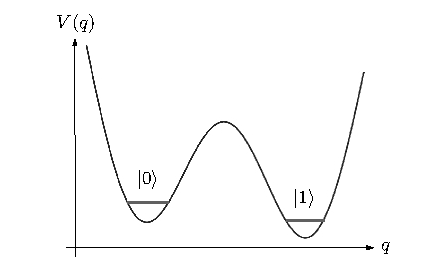
\includegraphics[width=.6\linewidth]{figures/ch05_fig01.pdf}
\caption{二状態系への写像。広がりをもつ座標$q$で記述され、二重井戸ポテンシャル$V(q)$の中を運動する系を考える。多くの場合、系は各井戸の最も低い状態だけを占有し、したがって、左と右の井戸への局在にそれぞれ対応する二つの基底状態$|0\rangle$、$|1\rangle$によって実効的に記述できる。}\label{fig:5.1}
\end{figure}
このような二準位系は量子計算において特に重要であり、量子情報を符号化する量子ビットの物理的実現となる（第7章参照）。

二準位系に固有の運動は、井戸の間の量子トンネル効果から生じ、二つの状態$|0\rangle$と$|1\rangle$の間の遷移をもたらす。状態$|0\rangle$、$|1\rangle$をPauliの$z$スピン演算子$\hat\sigma_z$の固有状態とすれば、トンネル効果は、系のHamiltonianに含まれる
\begin{equation}
\hat H_{\mathrm S}^{\mathrm{tunnel}}=-\frac12\Delta_0(|0\rangle\langle1|+|1\rangle\langle0|)\equiv-\frac12\Delta_0\hat\sigma_x
\tag{5.1}
\end{equation}
という形の項によって媒介される。$\Delta_0$は、いわゆるトンネル行列要素である。二つの井戸の基底状態間のエネルギー差（いわゆる「非対称エネルギー」）は、しばしば、各井戸内の状態のエネルギー間隔と比べて小さく、したがって各井戸の低いエネルギー準位は、ほぼ同じ高さに並ぶ。これにより、一方の井戸、例えば状態$|0\rangle$に対応する左の井戸に局在していた「粒子」が障壁をトンネルしても、通常、右の井戸の励起準位$|1'\rangle\ne|1\rangle$には到達できないことが保証される\cite{ref209}。

\subsubsectionlink{環境の写像}
次に、環境の写像へ移ろう。先に述べたように、ここで関心のある状況は二つある。環境を調和振動子の集まりとして記述する場合と、量子二準位系を表すスピン$1/2$粒子の集まりとして記述する場合である。

% 原文 p.175
\hypertarget{srcpage:175}{}\label{srcpage:175}
\subsubsectionlink*{振動子環境}
多数の調和振動子による環境の表現には、量子電磁力学やスピン波・電子気体模型にさかのぼる長い歴史がある（概観は文献\cite{ref210}参照）。振動子環境は、非局在化したボソン場のモードの準連続体に対応し、中心系のコヒーレンスとエネルギーは、この広がったボソン環境へ、実効的に不可逆に失われていく。「非局在化したモード」とは、個々の調和振動子、すなわち各ボソン場モードの波動関数が、広い空間領域に広がっていることを意味する。この環境モードの非局在性は、調和振動子環境に特有の性質である。

振動子環境は、主としてその一般性の高さのため、デコヒーレンス過程の模型化において、きわめて重要な役割を果たす。十分低いエネルギーでは、相互作用する系と環境の組合せの広いクラスを、調和振動子の環境へ線形に結合した、一つか二つの系の座標で実効的に表せることが示せる。実際、FeynmanとVernon\cite{ref211}が最初に示したように（CaldeiraとLeggettの研究\cite{ref212}も参照）、相互作用が十分弱く、2次摂動論が適用できれば、どのような環境との相互作用も、振動子環境へ線形に結合した系に、厳密に写像できる（この写像は後の5.4.2節で詳しく論じる）。

\subsubsectionlink*{スピン環境}
低温の状況では、通常、スピン環境が適切な模型となる。もちろん、こうした低温は、身の回りの日常世界で通常見られるものではない。しかし実験室では日常的に達成され、多くの実験に不可欠である。特に、巨視的な量子コヒーレンスとデコヒーレンスの研究を目指す実験（第6章参照）、中でも超伝導系を用いるもの（6.3節）を動作させるには、絶対零度に近い温度が必要となる。これらの実験は、量子計算機の実装に用いる量子ビット系の実現という点でも、大きな関心の対象である（第7章）。

したがって、低温領域のデコヒーレンスを正しく模型化することは非常に重要である。実験的証拠によれば、この領域のデコヒーレンスは、通常、常磁性スピン、常磁性電子不純物、トンネルする電荷、欠陥、核スピンなど、局在したモードとの相互作用に支配される\cite{ref199,ref200,ref213}（6.3節、6.4.2節も参照）。これらのモードが局在しているとは、振動子環境とは対照的に、各モードに付随する波動関数が、空間の小さな領域に閉じ込められていることを意味する。

% 原文 p.176
\hypertarget{srcpage:176}{}\label{srcpage:176}
各局在モードは、有限のエネルギーカットオフをもつ有限次元Hilbert空間で記述される。したがって、これらのモードを離散状態の集合として模型化し、スピン系へ写像できる。大部分の関心ある場合には、関係する状態は二つだけなので、局在モードの環境をスピン$1/2$粒子の環境へ写像できる。スピン環境のモードは、対象となる物理系自体の一部（「内部環境」を構成する）でも、周囲の基板の一部でもよい。例えば、いわゆる超伝導量子干渉素子（SQUID。詳細は6.3節参照）では、磁束座標は、SQUIDのバルク物質を構成し、磁束の侵入長内にある膨大な核スピンの集まりだけでなく、物質内のあらゆる不純物にも、電磁気的に結合する\cite{ref214}。

スピン環境が、重要で、しばしば支配的なデコヒーレンス源であることを示す例は、ほかにも数多い。巨視的尺度のコヒーレントな重ね合わせ状態を作ろうとするとき、研究者は、熱的環境を「凍結」させてデコヒーレンス効果を最小にするため、通常、非常に低い温度で実験を行う。この熱的環境こそ、先に述べた非局在化したボソンモード、すなわち調和振動子の浴である。しかし、SQUIDなどの超伝導系でしばしば行うように、温度を絶対零度の近傍まで下げても、物質内に本来存在する核スピンや不純物などの局在モードの影響は、通常変わらない。そのため、これらのデコヒーレンス源が、この低温領域で支配的になる。

\subsubsectionlink*{振動子環境とスピン環境：相違点と類似点}
振動子環境とスピン環境を用いる物理的動機を別々に概説したので、次に、両者の重要な相違点と類似点を論じ、説明をまとめよう。

先に述べたように、弱結合極限では振動子環境は普遍的な環境となる。任意の環境と系の相互作用を、同等な振動子環境への線形結合へ写像できる\cite{ref211,ref212}。この意味で、線形に結合した振動子環境は、弱結合極限の妥当性を前提としているともいえる。さらに、各モードの結合強度は、通常、環境の振動子数$N$に対して$\propto1/\sqrt N$とスケールすると仮定する。このスケーリングにより、すべてのモードの寄与を足し合わせた値は$N$に依存しなくなり、したがって熱力学的極限$N\longrightarrow\infty$が明確に定義される。

結合が弱く、$N$に依存するという、この組合せの仮定は、中心系は一般に環境の振動子の集団的影響を強く受ける一方、環境の個々の振動子は、系との結合から無視できるほど小さな影響しか受けないことを意味する。

% 原文 p.177
\hypertarget{srcpage:177}{}\label{srcpage:177}
中心系が環境に及ぼした効果は、通常非常に速く減衰する（これは4.2節で導入したBorn--Markov近似に対応する）。したがって、環境自身の運動は、中心系の運動からほとんど影響を受けない。

しばしば強調されるように\cite{ref199,ref200,ref210,ref215,ref216}、弱く、$N$に依存する結合という仮定は、スピン環境で表す局在モードの場合、通常は物理的に妥当でない。多くの物理的に興味ある状況で、個々の環境スピンと、通常は巨視的な中心系の座標との結合の強さに付随するエネルギー尺度は、Hamiltonianの残りの項で定まる他のエネルギー尺度に優越する。特に、環境のスピン間相互作用は、通常極端に弱い。異なる環境モードの波動関数が局在し、空間的な重なりがわずかしかないためである。環境スピンは、位相空間が制限されているため、他の外部の非局在モードにも、通常非常に弱くしか結合しない。さらに、スピン環境の場合、振動子環境のように結合を$N$に強く依存させてスケールすることは、通常、必要でも物理的に妥当でもないと論じられている\cite{ref199,ref200}（ただし文献では、$\propto1/N$などのスピン結合のスケーリングが、時に仮定されている。例えば文献\cite{ref217}参照）。

したがって、スピン環境で関心があるのは、環境のスピン数に依存しない、またはごく弱くしか依存しない結合係数で記述される強結合領域である。これにより、環境、ひいてはそれに結合する系は、振動子環境の場合と非常に異なる振る舞いを示す。通常、スピン環境のモードは、中心系を記述する関係座標に非常に強く「従属」するようになり、したがって環境の運動は中心スピンの運動から大きな影響を受ける\cite{ref199}。

この振る舞いは、環境内の固有の揺らぎ、すなわち自己Hamiltonianとスピン間相互作用による運動が凍結する零温度極限においてさえ、環境の動的変化を可能にする。この効果の帰結の一つとして、先に述べたように、絶対零度に近い温度、例えば$\mu\mathrm K$でも、スピン環境は通常、系に顕著なデコヒーレンス作用を及ぼす。一方、振動子浴のデコヒーレンス効果は、そのような温度では大部分の場合、比較して無視できるほど小さくなる。したがって、零度近くで比較的速いデコヒーレンス率を実験で観測したなら、局在モードとの相互作用が主要なデコヒーレンス源であることが示唆される。これにより、非局在化したボソン場モードと、局在したスピン型モードという、二つのデコヒーレンス源を、実験的に区別できる。

% 原文 pp.178--187
% 原文 p.178
\hypertarget{srcpage:178}{}\label{srcpage:178}
\subsectionlink{量子Brown運動}
量子Brown運動の模型は、空間の一次元を運動する粒子が、温度$T$で熱平衡にある独立な調和振動子の環境と、線形に相互作用するものである。量子Brown運動は、おそらく最も重要で、最もよく研究されているデコヒーレンス模型である。特に日常世界の巨視的尺度でデコヒーレンス効果を見積もる際の標準的な選択となるだけでなく、散逸的な量子系の一般的研究でも、きわめて重要な役割を果たす\cite{ref018,ref218}。したがって、この量子Brown運動を、少し時間をかけて調べることにする。

以下の順に進む。まず5.2.1節では、第4章で展開した形式を用い、この模型のBorn--Markovマスター方程式を導く。5.2.2節では、中心粒子が調和振動子ポテンシャルに閉じ込められる特別な場合のマスター方程式を論じる。5.2.3節では、環境の性質を記述する、いわゆるスペクトル密度の特定の形に注目し、得られたマスター方程式をさらに評価する。5.2.4節では、高温環境という特別な場合を考え、デコヒーレンスの研究で中心的役割を果たす、対応するCaldeira--Leggettマスター方程式を導く。5.2.5節では、位相空間の二つのGaussian波束の重ね合わせの時間発展を調べ、量子Brown運動の動力学を解析する。環境との相互作用によって、位相空間で局在した優先状態が出現する仕組みを示す。これらの指針状態の動的な発展は、Newton軌道の「量子版」に対応する。Caldeira--Leggett模型（および量子Brown運動の一般的模型）の結果を過度に一般化することへの注意を、5.2.6節でいくつか述べる。最後の5.2.7節では、量子Brown運動の厳密なマスター方程式を簡単に論じる。

\subsubsectionlink{Born--Markovマスター方程式の導出}
まず模型を定義しよう。通常どおり、系と環境の全Hamiltonian $\hat H$を三つの部分に分解する［(2.85)、(4.12)参照］。
\chfiveeq{2}
当面、系の自己Hamiltonian $\hat H_{\mathrm S}$は指定しない（後の5.2.2節では調和振動子ポテンシャルの場合に限定する）。環境の自己Hamiltonian $\hat H_{\mathrm E}$は、調和振動子の集まりを記述する。

% 原文 p.179
\hypertarget{srcpage:179}{}\label{srcpage:179}
仮定により、これらの振動子は互いに相互作用しないので、$\hat H_{\mathrm E}$は単に個々の振動子のHamiltonianの和、すなわち
\chfiveeq{3}
となる。明らかな記法で、$m_i$、$\omega_i$は第$i$環境振動子の質量と固有振動数、$\hat q_i$、$\hat p_i$は正準位置演算子と運動量演算子を表す。

系と環境の相互作用の形は、中心粒子（系S）の位置座標$\hat X$が、環境の振動子の位置$\hat q_i$に、結合強度$c_i$で線形に結合するものである。したがって、相互作用Hamiltonian $\hat H_{\mathrm{int}}$は
\chfiveeq{4}
と書ける。$\hat X$、$\hat q_i$の両方に線形である双線形結合の仮定は、模型の重要な仮定であり、このため、しばしば「線形量子Brown運動」と明示的に呼ばれる。以下の議論は、最も一般的に研究される、この模型に基づく。

系と環境の相互作用は、環境が系の位置座標を連続的に監視することを記述する、(2.91)の形をしている。したがって、さらに計算をしなくても、結合(5.4)は、散逸効果や他の基底でのデコヒーレンスなど、ほかに生じうる帰結とともに、系の位置基底でのデコヒーレンスをもたらすと、すでに予想できる。

最初の目標は、環境自己相関関数(4.10)の決定である。$\hat H_{\mathrm{int}}$［(5.4)参照］には一項しかないので、計算すべき関数も一つだけ、すなわち\footnote{前の第4章と同様、本章全体を通じて、密度演算子以外の、陽な時間引数をもつ演算子は、すべて相互作用描像の演算子と理解する約束を用いる。}
\chfiveeq{5}
である。ここで$\hat\rho_{\mathrm E}=\hat\rho_{\mathrm E}(0)$［(4.6)参照］である。(5.4)を用いて評価すると
\chfiveeq{6}
を得る。表記を簡単にするため、ここでは、環境の異なる部分に属する演算子の積におけるテンソル積記号「$\otimes$」を省略した。本章を通じて、引き続き省略する。

% 原文 p.180
\hypertarget{srcpage:180}{}\label{srcpage:180}
(5.6)の最後の段階で$i\ne j$の項が消えるのは、環境振動子が互いに相互作用せず、したがって完全に無相関だからである。したがって$i\ne j$に対して
\chfiveeq{7}
となる。振動子の位置座標の期待値$\langle q_i\rangle_{\hat\rho_{\mathrm E}}$がゼロであることを用いた。

こうして、$C(\tau)$を評価する作業は、平均$\langle\hat q_i(\tau)\hat q_i\rangle_{\hat\rho_{\mathrm E}}$［(5.6)参照］を計算する作業に帰着した。これは容易に行える。$\hat q_i$を、ボソンの生成・消滅演算子$\hat a_i^{\dagger}$、$\hat a_i$で表す表示へ移ろう。
\chfiveeq{8}
すると、相互作用描像での$\hat q_i$の時間発展は、［(A.4)参照］
\chfiveeq{9}
と書ける。したがって
\chfiveeq{10}
である。しかし量
\chfiveeq{11}
は、単に環境の第$i$振動子の平均占有数にすぎない。仮定により環境は熱平衡にあり、これは
\chfiveeq{12}
に対応する。この表式と、演算子$\hat a_i$、$\hat a_i^{\dagger}$の標準的な交換関係$[\hat a_i,\hat a_i^{\dagger}]=1$を用いると、(5.10)を
\chfiveeq{13}
と書き換えられる。

% 原文 p.181
\hypertarget{srcpage:181}{}\label{srcpage:181}
最後の段階では［(5.12)参照］
\chfiveeq{14}
を用いた。よって、環境自己相関関数(5.6)は
\chfiveeq{15}
と書ける。ここで関数
\chfiveeq{16_17}
は、文献では一般に、それぞれ雑音核、散逸核と呼ばれる。(5.16)の第1行の波括弧$\{\cdot,\cdot\}$は、反交換子$\{\hat A,\hat B\}\equiv\hat A\hat B+\hat B\hat A$を表す。(5.16)、(5.17)の最後の行で導入した関数$J(\omega)$は
\chfiveeq{18}
と定義され、環境のスペクトル密度と呼ばれる。スペクトル密度は環境の物理的性質をまとめたものであり、デコヒーレンスの理論的・実験的研究できわめて重要な役割を果たす。環境の模型化では、離散的振動数$\omega_i$、質量$m_i$をもつ個々の振動子による記述を、環境の振動数$\omega$の連続スペクトルに対応するスペクトル密度$J(\omega)$に置き換える、環境の連続極限へ移ることが多い。

% 原文 p.182
\hypertarget{srcpage:182}{}\label{srcpage:182}
そのような連続スペクトル密度の例は、後で論じる。当面は、$J(\omega)$の元の表式(5.18)を用いる。したがって、この段階で定義(5.18)の利点は、雑音核と散逸核(5.16)、(5.17)の記法が、いくらか簡潔になるだけである。

環境自己相関関数$C(\tau)$［(5.15)参照］を決定できたので、目標とする量子Brown運動のBorn--Markovマスター方程式の導出の主要な段階は終わった。残りの導出は容易である。演算子$\hat B$、$\hat C$［(4.9a)、(4.9b)参照］は、直ちに
\chfiveeq{19a_19b}
と書ける。ここで
\begin{equation}\hat X(\tau)=e^{\mathrm i\hat H_{\mathrm S}\tau}\hat Xe^{-\mathrm i\hat H_{\mathrm S}\tau}\tag{5.20}\end{equation}
は、相互作用描像における系Sの位置演算子である。$C(\tau)$を(5.15)で与え、(5.19a)、(5.19b)を、Born--Markovマスター方程式の一般式(4.8)へ代入すると、
\chfiveeq{21}
を得る。雑音核と散逸核(5.16)、(5.17)による分解$C(\tau)=\nu(\tau)-\mathrm i\eta(\tau)$［(5.15)参照］を用いて項を整理すると、マスター方程式の最終形
\chfiveeq{22}
を得る。環境によるデコヒーレンス（および散逸）の影響は、雑音核と散逸核(5.16)、(5.17)に、系のSchrödinger描像と相互作用描像の位置演算子の積を掛けたものの積分によって、完全に記述されることがわかる。

\subsubsectionlink{中心系としての調和振動子}
マスター方程式(5.22)をさらに簡単にし、雑音項と散逸項の物理的意味を理解するため、ここからは、標準的な自己Hamiltonian
\chfiveeq{23}
をもつ調和振動子で系を表す場合に限定しよう。

% 原文 p.183
\hypertarget{srcpage:183}{}\label{srcpage:183}
相互作用描像の位置演算子$\hat X(\tau)$［(5.20)参照］の具体的な形は、系の演算子$\hat X$、$\hat P$についてのHeisenberg運動方程式を解けば容易に求まり、
\chfiveeq{24}
となる。この$\hat X(\tau)$の表式を(5.22)に代入すると、調和振動子の熱環境に線形かつ弱く結合した調和振動子の、縮約された運動を記述するBorn--Markovマスター方程式
\chfiveeq{25}
を得る。ここでは、係数$\widetilde\Omega^2$、$\gamma$、$D$、$f$を
\chfiveeq{26a_26b_26c_26d}
と定義した。これらの係数には、マスター方程式(5.25)における役割から、それぞれ特定の物理解釈がある。各項を一つずつ論じる前に、文献でよく用いられる、他の二つの同値な形へ(5.25)を書き換えよう。

第一に、(5.25)を位置表示で表すことが、しばしば便利である。基本的関係
\chfiveeq{27}
を用いると、位置基底における縮約密度行列$\rho_{\mathrm S}(X,X',t)$の運動方程式
\chfiveeq{28}
を得る。

% 原文 p.184
\hypertarget{srcpage:184}{}\label{srcpage:184}
また、位置空間の縮約密度行列$\rho_{\mathrm S}(X,X')$のWigner表示$W(X,P)$［(2.132)と2.15.2節参照］についてのマスター方程式として、(5.25)を表すこともできる。ここでは導出を示さず、結果だけを述べる\cite{ref219}。
\chfiveeq{29}
統計力学に馴染みのある読者は、(5.29)と、古典統計物理のFokker--Planck方程式との形式的な類似性に気づくかもしれない。

マスター方程式(5.25)に現れる各項の解釈を論じよう。(5.25)の右辺の最初の交換子
\chfiveeq{30}
は、物理的振動数$(\Omega^2+\widetilde\Omega^2)^{1/2}$の調和振動子の、可逆でユニタリーな運動を記述する。したがって$\widetilde\Omega^2$は、中心振動子の固有振動数$\Omega$に、温度に依存しないシフトを導入する。これは155ページで述べたLambシフトの寄与の一例である。

次に、(5.25)の項
\begin{equation}-\mathrm i\gamma[\hat X,\{\hat P,\hat\rho_{\mathrm S}(t)\}]\tag{5.31}\end{equation}
は、環境との相互作用による運動量減衰、したがって散逸を記述する。これを見るため、運動方程式(5.25)で決まる、中心振動子の運動量期待値$\langle\hat P\rangle_t$の時間発展を考えよう。トレース則$\langle\hat P\rangle=\operatorname{Tr}_{\mathrm S}(\hat\rho_{\mathrm S}\hat P)$を用いると
\chfiveeq{32}
を得る。第1項$-M(\Omega^2+\widetilde\Omega^2)\langle\hat X\rangle_t$は、Lambシフトした調和振動子ポテンシャルにおける、通常のユニタリーな発展による。当面、このユニタリーで非散逸的な項を無視しよう。すると、(5.32)より、環境との相互作用によって、中心系の運動量期待値が率$2\gamma$で指数関数的に減少することが直ちにわかる。
\chfiveeq{33}
したがって、マスター方程式(5.25)の項(5.31)は、確かに$\gamma$に比例する率の運動量減衰を記述する。この率はスペクトル密度のみに依存し、環境の温度には依存しない［(5.17)、(5.26b)参照］。

% 原文 p.185
\hypertarget{srcpage:185}{}\label{srcpage:185}
次に、(5.25)の右辺の第3項
\chfiveeq{34}
を考えよう。この項は、Lindbladの二重交換子の形(4.45)であり、環境による系の位置座標$\hat X$の監視、したがって位置基底のデコヒーレンスを記述する。この役割は、位置表示で二重交換子を書き下しても容易にわかる。
\chfiveeq{35}
読者は、右辺の項が、第3章で論じた環境散乱模型で空間的局在化を記述した表式(3.55)と、同様の形をしていることに気づくかもしれない。したがって、係数$D$と$(X-X')^2$の積は、デコヒーレンス率として働く。すなわち
\chfiveeq{36}
は、距離$|X-X'|$にわたる空間的干渉が$e$分の1に抑制される時間尺度である［(3.58)も参照］。

係数$D$は、系の運動量の二乗の期待値$\langle\hat P^2\rangle_t$の時間発展からわかるように、運動量の拡散も記述する。(5.32)を得たのと同様の簡単な計算から
\chfiveeq{37}
を得る。$D$の項だけによる$\langle\hat P^2\rangle_t$の時間依存性に注目すると、$\langle\hat P^2\rangle_t\propto Dt$という発展を得る。これは、$D$が確かに運動量空間の拡散を記述することを示す。したがって、量子Brown運動の文献では、$D$はしばしば通常拡散係数と呼ばれる。ここで「通常拡散」という用語は、$\langle\hat P^2\rangle_t$の線形な時間依存性を指す。

このような通常拡散は、古典的Brown運動の特徴であることを思い出そう。そこでは、粒子の可能な位置を記述する正規分布の分散$\sigma_x^2$が、$\sigma_x^2(t)\propto t$と増大する。実際、同じ時間依存性は量子の場合にも成り立つ。長時間極限$\gamma t\gg1$において、マスター方程式(5.25)が位置空間の分散に対して
\chfiveeq{38}
という時間依存性を与えることは容易に示せる。すなわち、位置空間アンサンブルの幅$\Delta X(t)$は、古典的Brown運動と同様、漸近的に$\Delta X(t)\propto\sqrt t$とスケールする。

% 原文 p.186
\hypertarget{srcpage:186}{}\label{srcpage:186}
実際、量子と古典のこの類似性が、もともと「量子Brown運動」という用語を選ぶ動機となった。ちなみに、$\langle\hat P^2/2M\rangle$は系の運動エネルギーなので、(5.37)は、係数$\gamma$が散逸を定量化するという先の結果(5.33)も確認する。

拡散係数としての$D$の役割は、Wigner表示のマスター方程式(5.29)からもわかる。$D$の項だけを取り出すと、発展方程式
\chfiveeq{39}
を得る。これは、一定の拡散係数$D$をもつ場合の、変数$P$についてのよく知られた拡散方程式の形である。

最後に、マスター方程式(5.25)の最終項
\chfiveeq{40}
に注目しよう。この項も、通常拡散項(5.34)と同様に、拡散とデコヒーレンスを記述する。このことは、マスター方程式のWigner形(5.29)から最もよくわかる。$f$の項だけの寄与は
\chfiveeq{41}
である。右辺に二重微分が現れる点で、この形は拡散方程式(5.39)に似ている。しかし、「通常の」拡散方程式と異なり、(5.41)の二重微分は、異なる二つの変数$X$、$P$についての1階微分で構成される。この違いから、文献では量$f$を、しばしば異常拡散係数と呼ぶ。後で示すように、多くの物理的に興味ある状況では、系の縮約された運動に対する異常拡散項(5.40)の影響は、通常拡散項(5.34)と比べて無視できるほど小さい。そのような場合、異常拡散項を除いた、マスター方程式(5.25)の簡単な形を用いてよい（5.2.4節参照）。

この模型では、通常拡散係数と異常拡散係数は、スペクトル密度$J(\omega)$と環境温度$T$の両方に依存する［(5.16)、(5.17)を用いた(5.26)参照］。これは、前述のように環境温度に依存しない、振動数シフト$\widetilde\Omega^2$と運動量減衰率$\gamma$とは対照的である。

最後に、文献では、係数(5.26)の部分的に「前Markov的」な形もしばしば論じられることに触れておく（例えば文献\cite{ref015,ref016}）。この場合、時間積分の上限をまだ無限大とせず、時刻$t$までにとどめる（163ページの議論も参照）。言い換えれば、陽な時間依存性をもつ係数$\widetilde\Omega^2(t)$、$\gamma(t)$、$D(t)$、$f(t)$、
\chfiveeq{42a_42b_42c_42d}
を考える。

% 原文 p.187
\hypertarget{srcpage:187}{}\label{srcpage:187}
「Markov的な係数」(5.26)の代わりに、これらの時間依存係数で評価したマスター方程式(5.25)は、4.2.2節で述べたRedfield型\cite{ref174,ref175}となる。すなわち、このマスター方程式は、(i)Born近似、(ii)Bornマスター方程式(4.32)の右辺の被積分関数で、遅延時刻の密度演算子$\hat\rho^{(\mathrm I)}_{\mathrm S}(t')$を$\hat\rho^{(\mathrm I)}_{\mathrm S}(t)$に置き換える、最初のMarkov近似に基づく。ただし、(4.32)の積分範囲は無限大に延ばさない。

得られたマスター方程式、すなわち係数を(5.42)で与えた(5.25)は、例えば低温環境の場合など、Markov近似が完全には適切でない状況で、量子Brown運動をより現実的に扱える\cite{ref109,ref220}。実際、係数(5.42)は、一方のMarkov的な設定［時間に依存しない係数(5.26)で評価したマスター方程式(5.25)］と、他方の量子Brown運動の厳密なマスター方程式（5.2.7節参照）の中間に位置する。後者は、ここで考える弱結合極限だけでなく、任意の系・環境相互作用の強さで有効である。

係数(5.42)の時間依存性は、文献で詳しく研究されている（例えばHu、Paz、Zhang\cite{ref219}およびPaz、Zurek\cite{ref015}の議論）。例えば、環境がOhmicなスペクトル密度をもつ場合（次の5.2.3節参照）、振動数シフト$\widetilde\Omega^2(t)$と運動量減衰係数$\gamma(t)$は、ともにゼロから始まり、環境に顕著な割合で存在する最高振動数の大きさによって定まる時間尺度で、最終値へ漸近することが示せる。拡散係数$D(t)$、$f(t)$は、温度に依存しない初期過渡応答を示した後、温度に依存する漸近値へかなり速く落ち着く。

Markov的な係数(5.26)は、(5.42)の積分で極限$t\longrightarrow\infty$を取ることに対応するため、$\widetilde\Omega^2(t)$、$\gamma(t)$、$D(t)$、$f(t)$は、これらのMarkov的係数の値へ漸近する。以下では、Markov的な場合、すなわちマスター方程式(5.25)と、係数の時間に依存しない表式(5.26)に注目する。

% 原文 pp.188--194
% 原文 p.188
\hypertarget{srcpage:188}{}\label{srcpage:188}
\subsubsectionlink{Ohmicなデコヒーレンスと散逸}
中心系が調和振動子である量子Brown運動のマスター方程式(5.25)に現れる係数$\widetilde\Omega^2$、$\gamma$、$D$、$f$［(5.26)参照］を、さらに評価しよう。そのためには、$\nu(\tau)$、$\eta(\tau)$の表式［(5.16)、(5.17)参照］に入るスペクトル密度$J(\omega)$の、具体的な関数形を選ばなければならない。

前述のように、通常は、$J(\omega)$の元の表式(5.18)の離散的な和を、しばしば現象論的に動機づけられた、環境振動数$\omega$の連続関数に置き換える。一般に、$J(\omega)$の振動数依存性は、$J(\omega)\propto\omega^\alpha$というべき則に従うとする。指数$\alpha$の最も普通の選択は$\alpha=1$、すなわち$J(\omega)$が$\omega$とともに線形に増える場合である。この種類のスペクトル密度はOhmicと呼ばれる（名称は、スピン・ボソン模型の散逸効果の解析に由来する）。他の、より重要性の低い例として、$\alpha<1$のsubohmicなスペクトル密度と、$\alpha>1$のsupraohmicなスペクトル密度がある。

ここでは、Ohmicなスペクトル密度$J(\omega)\propto\omega$の場合に注目し、具体的に
\chfiveeq{43}
と書こう。定数$\gamma_0$は、系と環境の実効的な結合強度を記述する。スペクトル密度の元の離散的表式(5.18)では、この相互作用強度は、個々の振動子結合$c_i$を含む項の和で表されていた。まもなく見るように、$\gamma_0$は振動数に依存しない減衰定数として働く（具体的な実験状況に基づく現象論的なデコヒーレンス模型では、しばしば$\gamma_0$を測定データから導く）。

$J(\omega)$の振動数依存性がべき則ならば、環境の振動数分布は際限なく増大することになる。しかし、これは物理的に妥当ではない。通常、$J(\omega)$の$\omega$に対する線形依存性は、小さい$\omega$でしか成り立たず、高振動数へ向かって弱まる。そのため、普通は高振動数カットオフ$\Lambda$を選び、$\omega>\Lambda$の振動数で$J(\omega)$を減衰させる項を含めるように、(5.43)を修正する。よく用いられるのは、いわゆるLorentz--Drude形のカットオフ項である。
\chfiveeq{44}
このスペクトル密度のグラフを図5.2に示す。意図したとおり、カットオフ$\Lambda$を超える環境振動数$\omega$では、対応する振動数密度$J(\omega)$が減少する。

スペクトル密度$J(\omega)$の具体的選択(5.44)により、係数$\widetilde\Omega^2$、$\gamma$、$D$、$f$［(5.26)参照］を計算できるようになる。

% 原文 p.189
\hypertarget{srcpage:189}{}\label{srcpage:189}
\begin{figure}[htbp]\centering
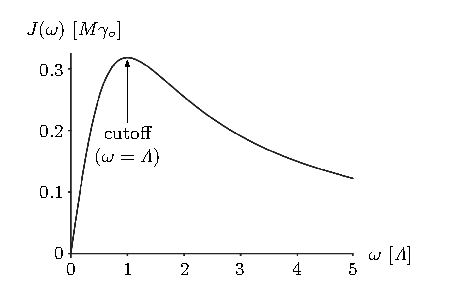
\includegraphics[width=.65\linewidth]{figures/ch05_fig02.pdf}
\caption{(5.44)のスペクトル密度$J(\omega)$のグラフ（単位：$M\gamma_0$）。$J(\omega)$は、高振動数カットオフ$\Lambda$より十分低い振動数$\omega$ではほぼ線形に増加し、その後$\omega>\Lambda$では減少する。振動数軸の単位はカットオフ$\Lambda$である。}\label{fig:5.2}
\end{figure}
運動量減衰係数$\gamma$と通常拡散係数$D$は、特に容易に評価できる。これを見るため、雑音核$\nu(\tau)$［(5.16)参照］は、前の因子$\sqrt{2/\pi}$がないことを除けば、関数$J(\omega)\coth(\omega/2k_{\mathrm B}T)$のFourier余弦変換にすぎないことに注意しよう。同様に、散逸核$\eta(\tau)$［(5.17)参照］は、$J(\omega)$のFourier正弦変換に比例する。さらに、$\gamma$の表式［(5.26b)参照］を見ると、これは$\eta(\tau)$のFourier正弦変換に比例している。

ところが、奇関数$g(-x)=-g(x)$に対して、2回のFourier正弦変換は元の関数を与える。
\chfiveeq{45}
スペクトル密度(5.44)は$\omega$の奇関数であり、$\gamma$は、前の因子を除けば$J(\omega)$を2回Fourier正弦変換したものなので、$\gamma$は、系の調和振動子の振動数$\Omega$で評価した$J(\omega)$に単純に比例する［(5.26b)、(5.45)と比較］。2回のFourier変換の定義(5.45)から生じる因子$2/\pi$を考慮すると、
\chfiveeq{46}
を得る。マスター方程式(5.25)の運動量減衰係数$\gamma$と、スペクトル密度の表式(5.43)で導入した実効結合強度$\gamma_0$とのこの関係は、$\gamma_0$を振動数に依存しない減衰定数とみなせるという、先の主張を正当化する。スペクトル密度にカットオフを課さなければ（$\Lambda\to\infty$）、$\gamma$と$\gamma_0$は厳密に等しい。

通常拡散係数$D$［(5.26b)参照］の計算も、同様の議論に従う。$D$は、$J(\omega)\coth(\omega/2k_{\mathrm B}T)$を2回Fourier余弦変換したものに比例する。

% 原文 p.190
\hypertarget{srcpage:190}{}\label{srcpage:190}
偶関数$g(-x)=g(x)$に対しては、このような2回のFourier余弦変換について、(5.45)と類似の恒等式
\chfiveeq{47}
が成り立つ。関数$J(\omega)\coth(\omega/2k_{\mathrm B}T)$は、確かに$\omega$について偶関数なので、
\chfiveeq{48}
を得る。$D$の温度依存性を図5.3に示す。$D$は温度とともに増大する。すなわち、環境の温度を上げるほどデコヒーレンスは強くなる。高温$k_{\mathrm B}T\gg\Omega$では、$\coth(\Omega/2k_{\mathrm B}T)\approx2k_{\mathrm B}T/\Omega$なので、$D$は温度にほぼ線形に増大する（この高温極限は後の5.2.4節で詳しく調べる）。

振動数の繰り込み$\widetilde\Omega^2$［(5.26a)参照］の表式は、Fourier正弦変換のFourier余弦変換である。この場合、(5.45)、(5.47)の形の簡単な恒等式はないが、この係数を具体的に評価するのは、かなり容易である。ここでは導出を示さず、結果だけを述べる。
\chfiveeq{49}
最後に、異常拡散係数$f$［(5.26d)参照］は、$\coth(\omega/2k_{\mathrm B}T)$の項があるため、評価がより難しい。比較的容易に扱えるのは、$k_{\mathrm B}T\gg\Omega$となる高温環境の場合である（次節参照）。この極限では、得られる$f$の表式は、通常拡散係数(5.48)に比べて、カットオフ振動数$\Lambda$程度の因子だけ小さい。
\begin{figure}[htbp]\centering
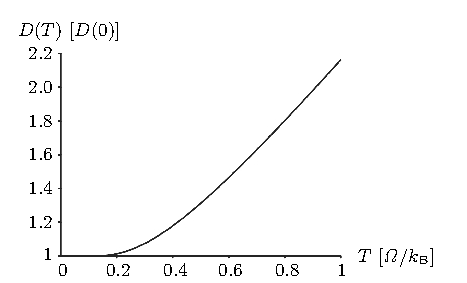
\includegraphics[width=.65\linewidth]{figures/ch05_fig03.pdf}
\caption{Ohmicなスペクトル密度(5.44)の場合の、通常拡散係数$D$［(5.48)参照］の温度依存性。縦軸の単位は、通常拡散係数の零温度値$D(T=0)$、温度軸の単位は$\Omega/k_{\mathrm B}$である。}\label{fig:5.3}
\end{figure}

% 原文 p.191
\hypertarget{srcpage:191}{}\label{srcpage:191}
\subsubsectionlink{Caldeira--Leggettマスター方程式}
以下では、高温環境の極限を詳しく調べよう。すなわち、環境の熱エネルギー$k_{\mathrm B}T$が、系の固有振動数$\Omega$と環境のカットオフ振動数$\Lambda$に対応するエネルギーより、はるかに大きい状況を考える。このとき、通常拡散係数$D$の表式(5.48)に現れる$\coth(\Omega/2k_{\mathrm B}T)$を、$2k_{\mathrm B}T/\Omega$で近似できる。これは、$\Omega/2k_{\mathrm B}T=0$のまわりの$\coth(\Omega/2k_{\mathrm B}T)$のTaylor展開の1次の項である。この場合、係数$D$は
\chfiveeq{50}
となる。また、環境振動数の上限領域であるカットオフ$\Lambda$は、系の特徴的振動数$\Omega$より、はるかに大きいと仮定する。すると(5.50)は
\chfiveeq{51}
という形になる。さらに、運動量減衰係数$\gamma$［(5.46)参照］は、実効結合強度$\gamma_0$の値に近づき、
\chfiveeq{52}
振動数の繰り込み$\widetilde\Omega^2$［(5.49)参照］は
\chfiveeq{53}
となる。最後に、ここで考える仮定のもとでは、異常拡散係数$f$を具体的に評価でき、
\chfiveeq{54}
を得る。

対応する異常拡散項$f[\hat X,[\hat P,\hat\rho_{\mathrm S}(t)]]$がマスター方程式(5.25)でどの程度重要かをさらに知るため、この項と$D[\hat X,[\hat X,\hat\rho_{\mathrm S}(t)]]$の大きさを比較しよう。その大きさは、それぞれ、およそ
\chfiveeq{55}
および
\chfiveeq{56}
である。

% 原文 p.192
\hypertarget{srcpage:192}{}\label{srcpage:192}
仮定により$\Lambda\gg\Omega$なので、ここではマスター方程式(5.25)の異常拡散項を、問題なく無視できる。

係数$D$、$\gamma$、$\widetilde\Omega^2$の上の表式(5.51)、(5.52)、(5.53)を、Born--Markovマスター方程式(5.25)へ代入しよう。結果は
\chfiveeq{57}
となり、系の、振動数をシフトしたHamiltonian $\hat H'_{\mathrm S}$は
\chfiveeq{58}
である。(5.57)の右辺に現れる項の解釈は、マスター方程式の、より一般的な形(5.25)について、すでに論じた（5.2.2節参照）。第1項は、振動数をシフトしたHamiltonianによる、通常のLiouville--von Neumann項である。第2項は、$\gamma_0$に比例する特徴的な率の運動量減衰、すなわち散逸を記述する。第3項は、位置基底のデコヒーレンスと、それに伴う運動量拡散を表し、その温度依存の特徴的な局在化率は、係数$M\gamma_0k_{\mathrm B}T$と、隔たりの二乗$(X-X')^2$の積で与えられる。

方程式(5.57)は、一般にCaldeira--Leggettマスター方程式として知られる（ここでは中心系が調和振動子の場合について書いた）。これは1980年代初頭に、CaldeiraとLeggettが経路積分法を用いて初めて導いた\cite{ref221}。デコヒーレンス過程と散逸過程の模型化に、広く用いられる。実際、導出の基礎となる仮定が厳密には満たされない状況でも、しばしばかなりうまく適用されてきた（例えば、$k_{\mathrm B}T\lesssim\Lambda$となることの多い量子光学の状況\cite{ref222}）。

Caldeira--Leggettマスター方程式の特に魅力的な性質は、デコヒーレンス率と、その率と散逸の関係する率との関係を、非常に直観的かつ簡単に見積もれることである。これを見るため、温度$T$の、質量$M$の粒子の熱的de Broglie波長が、通常どおり$\hbar\equiv1$とすると、［(2.114)参照］
\chfiveeq{59}
で与えられることを思い出そう。したがって位置表示を用いれば、(5.57)の右辺の最終項は
\chfiveeq{60}
と書ける。

% 原文 p.193
\hypertarget{srcpage:193}{}\label{srcpage:193}
この項は、［(3.58)、(5.36)と比較］
\chfiveeq{61}
というデコヒーレンス率$\tau_{|X-X'|}^{-1}$での空間的局在化を記述する。デコヒーレンス率と減衰率$\gamma_0$の比は、空間的隔たりと物体の熱的de Broglie波長(5.59)の比の二乗に等しいことがわかる。定数$\gamma_0^{-1}$は系の散逸（緩和）時間尺度を定量化するので、(5.61)は、2.11節で導出なしに与えた表式(2.113)そのものである。そこで述べたように、量子Brown運動模型から導かれる表式(5.61)は、1980年代初頭に、デコヒーレンス時間尺度という概念を導入するため、Zurekが初めて用いた\cite{ref012}。同じ節で、熱的de Broglie波長は巨視的物体、さらには中間的な大きさの物体でも極端に小さいと指摘した。したがって、巨視的に離れた重心位置の重ね合わせで記述される物体は、通常、緩和時間尺度より何桁も短い時間尺度で、デコヒーレンスを起こす。

したがって、デコヒーレンス時間程度の時間尺度では、マスター方程式(5.57)の散逸項を無視できる場合が多い。これにより、簡単化した「純粋デコヒーレンス」マスター方程式
\chfiveeq{62}
または、位置基底で表した
\chfiveeq{63}
を得る。この式は、(5.61)の率での空間的コヒーレンスの局所的減衰を記述する。(5.63)は、環境散乱の場合の運動方程式(3.78)と同じ構造をもつことに注意しよう。散乱模型の散乱定数$\Lambda$［(3.56)参照］の役割を、ここでは係数$\gamma_0/\lambda_{\mathrm{dB}}^2$が担う。二つの式(3.78)、(5.63)の違いは、(5.63)では中心系が調和振動子ポテンシャルに閉じ込められるのに対して、(3.78)の基礎となる散乱模型は、束縛されていない系を考えたという点だけである。

しかし、この違いは決定的なものではない。実際、Caldeira--Leggett方程式(5.57)の形は、系を調和振動子で表す仮定に結びついていないことがわかるからである。系の任意のポテンシャルについて、(5.57)の形の方程式を書ける。系は、正準位置座標$\hat X$と運動量座標$\hat P$によって記述される必要さえない。

% 原文 p.194
\hypertarget{srcpage:194}{}\label{srcpage:194}
代わりに、スピン・ボソン模型の場合（5.3節参照）のように、Pauliスピン演算子$\hat\sigma_x$、$\hat\sigma_z$で表す離散的な二準位系を、模型化の対象に選んでもよい。その場合、これらのPauliスピン演算子が、マスター方程式の座標$\hat X$、$\hat P$の代わりを務め、系の異なる物理的性質は、マスター方程式の係数に入る物理量の具体的選択に反映される。

% 原文 pp.194--203
\subsubsectionlink{量子Brown運動の動力学}
調和振動子で中心系を表す量子Brown運動のマスター方程式の一般形(5.25)に戻り、この方程式によって生成される系の時間発展を示そう。この運動は、多くの著者によって詳しく調べられている。ここでは主に、Paz、Habib、Zurek\cite{ref184}の解析に従う。

系の初期波動関数を、コヒーレントな重ね合わせ
\chfiveeq{64}
とする。$\Psi_1(X)$、$\Psi_2(X)$は
\chfiveeq{65}
で与えられるGaussian波束である。ここで$N$は規格化定数、$\delta$は位置空間でのGaussianの幅である。したがって、初め位相空間で対称に位置する二つのGaussian、すなわち、位置が$\pm X_0$で、大きさが同じ逆向きの運動量$P_0$をもつ二つのGaussianの重ね合わせを考えている。

この方法により、位置空間と運動量空間のデコヒーレンスの動力学を調べ、量子Brown運動のデコヒーレンスは運動量の重ね合わせにも作用するのか、それとも位置の重ね合わせだけに作用するのか、この二つの基底でデコヒーレンスの特徴的時間尺度はどう違うのか、といった重要な問いに取り組める。これに答えるため、関心のある二つの極限の場合のデコヒーレンスの動力学を考える\cite{ref184}。最初は、位置だけが離れた（$X_0>\delta$、$P_0=0$）二つのGaussianの重ね合わせ(5.64)、
\begin{equation}
\Psi_{\mathrm{pos}}(X,t=0)=N\left\{\exp\left[-\frac{(X-X_0)^2}{2\delta^2}\right]+\exp\left[-\frac{(X+X_0)^2}{2\delta^2}\right]\right\}
\tag{5.66}
\end{equation}
である。二つ目は、$\Psi_1(X)$と$\Psi_2(X)$の運動量だけが離れた（$X_0=0$、$P_0>1/\delta$）重ね合わせ(5.64)に対応する。
\chfiveeq{67}

% 原文 p.195
\hypertarget{srcpage:195}{}\label{srcpage:195}
いまは座標$X$、$P$で記述する位相空間の描像を用いているので、位置空間の密度行列$\rho_{\mathrm S}(X,X')=\Psi(X)\Psi^*(X')$のWigner表示$W(X,P)$［(2.132)参照］に移るのが便利である。Gaussian波束のWigner表示は、やはり$(X,P)$平面に局在したGaussianなので、初期状態(5.64)に対応するWigner関数は、かなり容易に計算できる。二つの直接項$\Psi_1(X)\Psi_1^*(X')$、$\Psi_2(X)\Psi_2^*(X')$のWigner表示は、次の形をもつことが示せる\cite{ref184}。
\chfiveeq{68}
非対角の干渉項$\Psi_1(X)\Psi_2^*(X')$、$\Psi_2(X)\Psi_1^*(X')$の寄与は、Wigner表示では
\begin{equation}
W_{\mathrm{int}}(X,P,t=0)=2N^2\delta^2\exp\left[-\frac{X^2}{\delta^2}-\delta^2P^2\right]\cos[2X_0P+2P_0X]
\tag{5.69}
\end{equation}
となる。したがって、初期状態(5.64)の完全なWigner関数は
\chfiveeq{70}
である。この関数を、位置だけ、運動量だけが離れている二つの極限、すなわち$\Psi_{\mathrm{pos}}(X,t=0)$［(5.66)参照］と$\Psi_{\mathrm{mom}}(X,t=0)$［(5.67)参照］について、図5.4の最上段に示す。二つの「古典的な」直接ピークが、それぞれ$X$軸と$P$軸に沿って局在している様子が、はっきりわかる（2.15.2節の一般的議論も参照）。また、これらのピークの間には、特徴的な振動模様が見える。その「山」と「谷」は、ピークを結ぶ軸、すなわち隔たりが生じている変数に対応する軸に平行である。(5.69)から明らかなように、振動の波数は、隔たり$X_0$と$P_0$によって直接決まる［(2.135)も参照］。

次に、Wigner表示で表したBorn--Markovマスター方程式(5.29)で与えられる、Wigner関数(5.70)のその後の時間発展を調べよう。ここでは導出の詳細に立ち入らないが、時間発展後のWigner関数も、やはり
\chfiveeq{71}
という形に書け、直接項と干渉項は
\chfiveeq{72a_72b}
で与えられることが示せる\cite{ref184}。

% 原文 p.196
\hypertarget{srcpage:196}{}\label{srcpage:196}
\begin{figure}[htbp]\centering
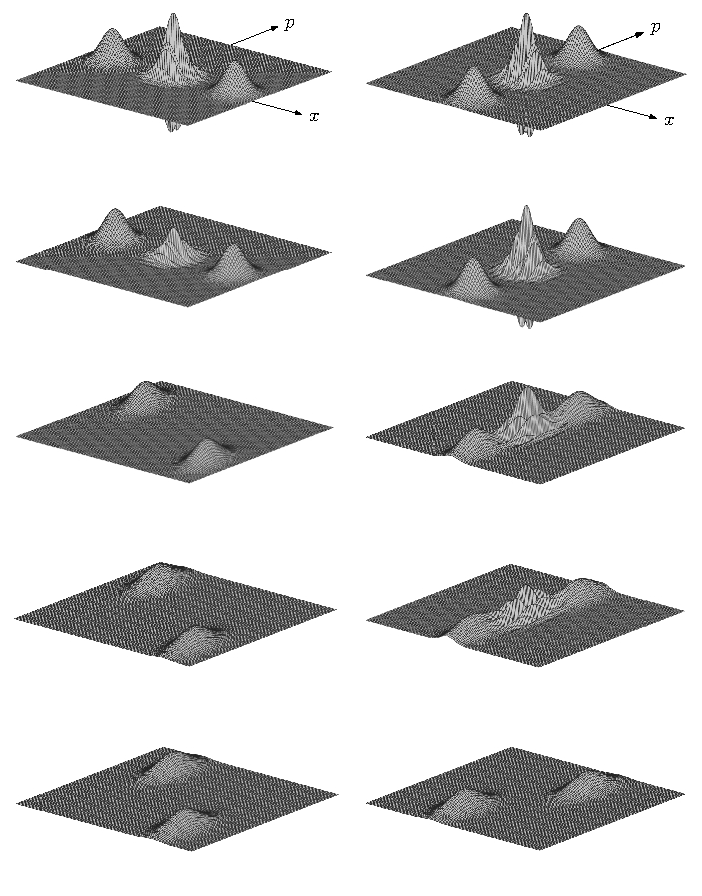
\includegraphics[width=.9\linewidth]{figures/ch05_fig04.pdf}
\caption{Paz、Habib、Zurek\cite{ref184}が調べた、Wigner描像での二つのGaussian波束の重ね合わせの時間発展。左列は、初期波束が位置だけ離れている場合、右列は、運動量だけ離れた波束の重ね合わせの動力学に対応する。二つの波束の干渉は、直接ピーク間の振動で表される。環境との相互作用は、この振動を減衰させ、この過程がデコヒーレンスを表す。ただし、この減衰は、二つの初期条件に対して異なる時間尺度で起こる。}\label{fig:5.4}
\end{figure}

% 原文 p.197
\hypertarget{srcpage:197}{}\label{srcpage:197}
ここで係数$\delta_1$、$\delta_2$、$X_{\mathrm c}$、$P_{\mathrm c}$、$\beta$、$A_{\mathrm{int}}$、$\kappa_x$、$\kappa_p$は、一般に時間依存であり、初期値は、［(5.72)と(5.68)、(5.69)を比較］
\chfiveeq{73a_73b_73c}
である。量子Brown模型の厳密解、すなわち上の扱いで用いたBorn--Markov近似を行わない解（後の5.2.7節参照）から得られる、これらの係数の具体的な、ただし非常に複雑な一般式は、環境のスペクトル密度の任意の選択に対して、Paz、Habib、Zurek\cite{ref184}が与えている。Born--Markov近似に注目し、スペクトル密度を特定の形に選べば、より簡単で具体的な表式が得られる。

いずれにせよ、ここでは係数の正確な形には、これ以上立ち入らない。代わりに、(5.71)、(5.72)が記述するWigner関数の時間発展の、十分な定性的描像を得よう。この発展は、二つの極限的な初期状態(5.66)、(5.67)について、図5.4に示されている。どちらの初期条件でも、環境との相互作用によって、波束の量子干渉を表す振動が抑制される。しかし、このデコヒーレンスが起こる時間尺度は、大きく異なる。初め位置だけ離れた二つの波束の重ね合わせ(5.66)は、運動量の重ね合わせ(5.67)より、はるかに速くデコヒーレンスを起こす。実際、後で詳しく解析するように、最初の場合、デコヒーレンスの時間尺度は、系の緩和時間尺度や力学的時間尺度に、事実上依存しない。これに対し、運動量の重ね合わせという二つ目の場合、量子干渉は、系の固有の運動、すなわち自己Hamiltonianが定める時間尺度で減衰する。

この観察は、かなり容易に説明できる。相互作用Hamiltonianは、系の位置に陽に依存する。これは、環境が位置を直接監視し、位置基底に強く速いデコヒーレンスをもたらすことを意味する。一方、系の運動量は相互作用Hamiltonianに現れないため、環境から直接監視されない。したがって運動量のデコヒーレンスは、位置の監視と、その結果の位置のデコヒーレンスを通じ、間接的にしか起こりえない。

% 原文 p.198
\hypertarget{srcpage:198}{}\label{srcpage:198}
波束が初め運動量だけ離れている場合、状態(5.67)は、すでに位置についてよく局在している。したがって、系の位置の環境監視は、この状態をさらに位置局在させることはできず、重ね合わせ(5.67)は初め、環境監視、ひいてはデコヒーレンスに敏感ではない。

しかし、二つの直接ピークに付随する逆向きの運動量$\pm P$が、そのピークを$X$の逆方向へ移動させるので、力学的時間尺度で、この重ね合わせは位置の重ね合わせへと発展する（図5.4の右列参照）。すると、状態は位置の環境監視に敏感になり、それが振動の減衰をもたらす。このことは、相互作用Hamiltonianに運動量項がないのに、なぜ運動量のデコヒーレンスが起こるのか、そして、なぜそれが、位置のデコヒーレンス、すなわち環境が直接監視する量のデコヒーレンスの、はるかに短い時間尺度ではなく、力学的時間尺度で起こるのかを説明する。以下では、Wigner関数(5.71)の直接項(5.72a)と干渉項(5.72b)に現れる量の時間依存性を解析し、この議論をより正確にする。

まず、直接項$W_{1,2}(X,P,t)$で記述するGaussianピークの運動を見よう。これらのピークは、$X(t)=\pm X_{\mathrm c}(t)$、$P(t)=\pm P_{\mathrm c}(t)$という「古典的」軌道をたどる。この軌道はスペクトル密度の具体的選択には依存するが、環境の温度には依存しない。Gaussianピークの幅は、$\delta_1$（位置幅）と$\delta_2$（運動量幅）で与えられ、環境の存在によって時間とともに変化する。また、環境はGaussianの形を歪ませ、その程度は係数$\beta$で定量化される。幅$\delta_{1,2}$と歪み$\beta$は、いずれも環境のスペクトル密度と温度に依存する。

デコヒーレンスの議論で最も興味があるのは、干渉項$W_{\mathrm{int}}(X,P,t)$［(5.72b)参照］であり、これは波束$\Psi_1(x)$と$\Psi_1(x)$の干渉を特徴づける振動を表す。まず、$X$軸、$P$軸に沿った振動の、温度に依存する波数$\kappa_x$、$\kappa_p$が、環境との相互作用で変わる。デコヒーレンスに最も関係する量は$\exp(-A_{\mathrm{int}})$であり、後で見るように、これは振動の減衰、したがってデコヒーレンスを記述する。この項は干渉縞の可視度を定量化すると解釈できる。$\exp(-A_{\mathrm{int}})$は、$X=P=0$で最大となる干渉項$W_{\mathrm{int}}(X,P)$と、$X=\pm X_{\mathrm c}$、$P=\pm P_{\mathrm c}$で最大となる直接項$W_{1,2}(X,P)$の、ピークの比に等しいからである。
\begin{equation}
\exp(-A_{\mathrm{int}})=\frac12\frac{W_{\mathrm{int}}(X=0,P=0)}{[W_1(X=X_{\mathrm c},P=P_{\mathrm c})W_2(X=-X_{\mathrm c},P=-P_{\mathrm c})]^{1/2}}.
\tag{5.74}
\end{equation}

% 原文 p.199
\hypertarget{srcpage:199}{}\label{srcpage:199}
この解釈から、$\exp(-A_{\mathrm{int}})$は、しばしば「干渉縞可視度関数」と呼ばれる。量$A_{\mathrm{int}}$は、次で与えられることが示せる\cite{ref184}。
\chfiveeq{75}
ここに現れる量は、すべて陽に時間依存すると理解する。時刻$t=0$では、$\delta_1=\delta_2=\delta$、$\kappa_x=P_0$、$\kappa_p=X_0$［(5.73)参照］なので、$A_{\mathrm{int}}=0$である。その後の時刻$t>0$では、$A_{\mathrm{int}}$は増大するが、常に、時間に依存しない漸近的な最大値
\chfiveeq{76}
によって上から抑えられる。実際、量子Brown運動のマスター方程式から、$A_{\mathrm{int}}$の具体的な運動方程式を導ける。結果は\cite{ref184}
\chfiveeq{77}
である。$D$と$f$は、Born--Markov近似での通常拡散係数と異常拡散係数である（Redfield方程式または厳密なマスター方程式\cite{ref219}を用いれば、これらは陽に時間に依存する。5.2.7節も参照）。

(5.77)は、$A_{\mathrm{int}}$の時間発展、したがって干渉項が抑制される動力学が、いくつかのパラメータに依存することを示す。まず、$A_{\mathrm{int}}$の時間変化は、拡散係数$D$、$f$に陽に直接依存するが、マスター方程式(5.25)の運動量減衰（摩擦）係数$\gamma$にも、繰り込まれたHamiltonian $\hat H'_{\mathrm S}$による自由発展にも、直接は依存しない。ただし、(5.77)の$\kappa_x$、$\kappa_p$の運動は$\gamma$と$\hat H'_{\mathrm S}$に依存するため、$A_{\mathrm{int}}$の時間発展も、これらから間接的に影響を受ける。

一方、後で見るように、$\gamma$と$\hat H'_{\mathrm S}$の間接的影響は、通常、拡散係数に対する直接的依存性と比べて非常に弱い。このことは、すでに重要な結論を示唆する。多くの場合、$A_{\mathrm{int}}$の発展、したがってWigner関数の振動項の抑制は、$\gamma$で定まる緩和時間尺度と、$\hat H'_{\mathrm S}$で決まる力学的時間尺度に、本質的に依存しない時間尺度で起こる。

(5.77)の右辺の第1項$4D\kappa_p^2$は非負なので、通常拡散係数$D$は、常に干渉項の抑制、したがってデコヒーレンスに対応する。(5.72b)より、$\kappa_p$は、運動量方向に沿ったWigner振動の波数を定量化する。(5.77)から明らかなように、第2項の符号は一定ではなく、$\kappa_x$と$\beta\kappa_p$の兼ね合いに依存する。したがって、異常拡散係数$f$は、干渉の抑制を助ける役割から、この抑制に対抗する役割へと変わることがある。

% 原文 p.200
\hypertarget{srcpage:200}{}\label{srcpage:200}
(5.77)が与える$A_{\mathrm{int}}$の時間発展の決定的な特徴は、初期条件、特に初期の隔たり$X_0$、$P_0$への直接的依存性である。この依存性は、時刻$t=0$で$\kappa_x=P_0$、$\kappa_p=X_0$となる係数$\kappa_x$、$\kappa_p$を通じて入る［(5.73b)参照］。以下で見るように、この依存性が、前述の、位置と運動量のデコヒーレンスの時間尺度の大きな違いを生む（図5.4も参照）。

まず、初期状態が、位置空間だけで離れた二つのGaussianの重ね合わせである極限(5.66)に注目しよう。$t=0$で$\kappa_p=X_0$なので、$A_{\mathrm{int}}$の発展方程式(5.77)の通常拡散項$4D\kappa_p^2$は、直ちに干渉の減衰に寄与する。

上の5.2.4節で論じた、高温のOhmic環境という簡単なCaldeira--Leggettの場合について、(5.77)の$A_{\mathrm{int}}$の時間依存性を調べよう。ここでは、異常拡散係数$f$は通常拡散係数$D$に比べて無視でき、$D$は$2M\gamma_0k_{\mathrm B}T$で近似できる［(5.51)参照］。さらに、干渉縞は時間とともにほとんど移動しない、すなわち$\kappa_p$の時間依存性を無視し、その初期値$X_0$で置き換えられるという、簡単化の仮定を置こう。この仮定のもとで、(5.77)は容易に解け、
\chfiveeq{78}
または、熱的de Broglie波長$\lambda_{\mathrm{dB}}=1/\sqrt{2Mk_{\mathrm B}T}$を用いて、
\chfiveeq{79}
を得る。したがって、Wigner関数の振動は、デコヒーレンス率
\chfiveeq{80}
で指数関数的に減衰する。$\Delta X$は位置空間のコヒーレントな隔たりである。こうして、Caldeira--Leggettの場合のデコヒーレンス率についての先の結果(5.61)を再び得る。

次に、Gaussianの重ね合わせが、初めは運動量だけ離れた、すなわち$X_0=0$である状況(5.67)を考えよう。$t=0$で$\kappa_p=0$なので、初めは$\mathrm dA_{\mathrm{int}}/\mathrm dt=0$となる。すなわち、$\kappa_p=0$がゼロから離れ始めるまで、$A_{\mathrm{int}}$は初期値ゼロにとどまり、この初期段階ではデコヒーレンスが起こらない。弱く減衰する系では、$\kappa_p$は$\kappa_p(t)\propto X_{\mathrm c}(t)$のように発展し、その値が直接ピークの軌道に従うことを示せる\cite{ref184}。したがって、$\kappa_p$の増加は$X_{\mathrm c}$の変化と結びつく。$X_{\mathrm c}$は初期値ゼロから始まり、力学的時間尺度で発展する。

% 原文 p.201
\hypertarget{srcpage:201}{}\label{srcpage:201}
すると、(5.77)の拡散項が$A_{\mathrm{int}}$に作用できるようになり、$A_{\mathrm{int}}$が正となって、Wigner干渉項$W_{\mathrm{int}}(X,P,t)$［(5.72b)参照］の振動が抑制される。

したがって、運動量だけ離れたGaussian波束の重ね合わせでは、デコヒーレンスは、二つの異なる時間尺度に関係する。第一は、位置の重ね合わせが生成される比較的遅い力学的時間尺度である。すなわち、$X_{\mathrm c}$が初期値ゼロから十分離れ、環境による系の位置の監視が作用できるようになる時間尺度である。第二に、位置の重ね合わせが動的に作られると、それは位置空間の重ね合わせのデコヒーレンス時間尺度（例えば高温Ohmic環境では(5.80)）で、急速にデコヒーレンスを起こす。したがって、運動量のデコヒーレンス率は、常に系の力学的発展の速さによって制限される。これは、運動量のデコヒーレンスに関係する時間尺度が、力学的時間尺度だけであることを意味する。この解析は、位置空間に比べて運動量空間のデコヒーレンスが、はるかに遅いという最初の直観的説明を、厳密に支える。

環境との相互作用によって選び出される優先状態、すなわち指針状態は、結局どのようなものだろうか。これに答えるため、調和振動子系の縮約密度行列$\hat\rho_{\mathrm S}$の純度$\varsigma=\operatorname{Tr}\hat\rho_{\mathrm S}^2$［(2.30)参照］の変化を計算できる。この変化はBorn--Markovマスター方程式(5.25)から求められる。ここでは、運動量減衰項$\gamma$の影響を無視する。この項は常に、密度行列の形にまったく依存しない、純度の非物理的な時間増加をもたらすことが示せるからである\cite{ref016}。この項の省略は、弱減衰の極限、すなわち「不足減衰」の調和振動子の場合には十分正当化できる。また、高温極限では適切である（5.2.4節参照）ため、異常拡散項も無視する。この仮定のもとで、純度の瞬間的変化は\cite{ref086}
\chfiveeq{81}
となる。$\Delta X^2(t)=\langle\hat X^2\rangle_t-\langle\hat X\rangle_t^2$は、位置空間の分散である。したがって、この空間分散を最小にすれば、純度の瞬間的減少、したがってデコヒーレンスの大きさも最小となる。すなわち、瞬間的な指針状態は、位置について完全に局在したものであろう。この結果は、環境が系の位置を直接監視することから、予想できたかもしれない。

しかし、自己Hamiltonian(5.23)で与えられる調和振動子系の固有の発展も、重要な役割を果たす。実際、調和振動子についてよく知られているように、一周期$T=2\pi/\Omega$の間に、位置と運動量は役割を入れ替える。

% 原文 p.202
\hypertarget{srcpage:202}{}\label{srcpage:202}
系のHamiltonianが位置変数と運動量変数についてもつこの対称性は、位相空間で非対称に局在する状態（例えば位置にはよく局在するが、運動量には完全に非局在化した状態）が、系のHamiltonianによる時間発展で大きく変わることを意味する。

この議論を正確にするため、純度の瞬間的変化(5.81)を調べる代わりに、調和振動子系の完全な一周期$t=0\ldots T$にわたって平均した、純度の変化を見よう。この平均変化は、次で与えられることが示せる\cite{ref015,ref084}。
\chfiveeq{82}
ここで$\Delta X^2\equiv\Delta X^2(0)$、$\Delta P^2\equiv\Delta P^2(0)$は、初期時刻$t=0$での位置と運動量の分散である。異常拡散項$f$は、(5.81)のようにあらかじめ無視しなくても、一周期でその影響が平均して消えるため、(5.82)に現れない。

(5.82)は、不確定性関係が課す$\Delta X\Delta P\geq1/2$の制約（本章を通じて$\hbar\equiv1$としたことを思い出そう）のもとで、右辺の括弧内を最小にするように$\Delta X^2$、$\Delta P^2$を選べば、純度の平均減少、したがってデコヒーレンスの大きさが最小になることを示す。純度の減少(5.82)を最小にする選択は
\chfiveeq{83}
であるとわかる。したがって、量子Brown運動で環境により超選択される指針状態は、位置と運動量の両方でよく局在する、最小不確定性Gaussian、すなわちコヒーレント状態である。これを最初に示したのはZurek、Habib、Paz\cite{ref086}である（文献\cite{ref084,ref223,ref224,ref225,ref226}も参照）。

もちろん、量子力学は位相空間での完全な局在化を禁じるが、環境との相互作用で選ばれるコヒーレント状態は、「これ以上よくはできない」位相空間局在を表す。したがって、このコヒーレント状態を、位相空間の古典的な一点という理想概念の、量子版とみなせる。縮約密度行列が記述する、最小不確定性Gaussian波束の非真正アンサンブルを、時間を追って同定し直すことで、位相空間における粒子の準Newton的な軌道を取り戻せる。

厳密にいえば、量子Brown運動の指針状態がコヒーレント状態であるという上の導出は、弱く減衰する調和振動子の仮定に基づく。しかし、強減衰領域でも結論は大きく変わらず、主な違いは、運動量より位置の局在が、より強く優先されることである\cite{ref227}。さらにEisert\cite{ref106}は、熱浴に結合した自由量子粒子の場合、最小不確定性Gaussian状態の環境誘起超選択は、完全に一般的であることを示した。

% 原文 p.203
\hypertarget{srcpage:203}{}\label{srcpage:203}
すなわち、任意の浴温度、系と環境の結合強度、環境スペクトル密度に対して、そのようなコヒーレント状態への厳密なデコヒーレンスが起こる。

最後に、環境の振動数が系の固有振動数に比べて非常に小さい極限についても、量子Brown運動の優先状態の環境誘起超選択を調べられる。この「遅い」環境の極限は、5.2.4節のCaldeira--Leggett模型の状況とは反対であり、デコヒーレンスの「量子極限」に対応する（2.8.2節参照）。PazとZurek\cite{ref103}は、標準的な量子Brown運動模型の変種、すなわちスカラー場と相互作用する粒子を考え、この極限では、縮約密度行列の純度の減少が、系のエネルギー固有状態、すなわち自己Hamiltonianの固有状態について最小となることを見いだした。したがって、それらが系の指針状態として出現する。この結果は、2.8節の一般的な議論と一致する。

% 原文 pp.203--206
\subsubsectionlink{量子Brown運動模型とCaldeira--Leggett模型の限界}
5.2.4節では、Caldeira--Leggett模型から、空間的デコヒーレンス率の見積もりについて、非常に簡単な式(5.61)が得られることを示した。特に、空間的デコヒーレンス率と散逸率の比は、コヒーレントな隔たりと熱的de Broglie波長の比によって与えられた。2.11節で示したように、中間的あるいは巨視的な大きさの物体が、同じく中間的・巨視的な距離だけ離れた二つの位置の重ね合わせで記述される、典型的状況では、この比は非常に大きくなりうる。これは、そのような状況では、典型的なデコヒーレンス率が、散逸率より何桁も大きくなることを示唆する。

しかし、このような見積もりを、あまり文字どおりに解釈しないよう注意すべきである。Caldeira--Leggett方程式(5.57)、したがってデコヒーレンス率の表式(5.61)を導いた仮定は、物理的に現実的で興味ある場合には、しばしば満たされない\cite{ref162,ref228,ref229}。したがって、(5.61)を、空間的重ね合わせのデコヒーレンス率について普遍的に成り立つ表式と解釈し、過度に一般化するのは適切でない。さらに、Caldeira--Leggett方程式(5.57)から生じる、デコヒーレンスと散逸の一般的な動力学は、この模型の文脈と範囲の中で考えるべきであり、この模型から得た結果から、過度に一般的な結論を引き出すことには慎重であるべきだ。

例えば、(5.61)のデコヒーレンス率は、位置空間の重ね合わせ状態のコヒーレントな隔たり$\Delta X=|X-X'|$の二乗に比例する。もちろん、隔たりが大きいほど重ね合わせは非古典的であり、デコヒーレンスも速くなると期待されるので、直観的には妥当である。

% 原文 p.204
\hypertarget{srcpage:204}{}\label{srcpage:204}
しかし、物理的には、このデコヒーレンス率には、隔たりをさらに増しても超えられない上限があるはずである。

この上限の理由は、第3章で論じた環境散乱の結果を思い出せば容易にわかる。そこでは、散乱される環境粒子の典型的波長が、コヒーレントな隔たり$\Delta X$に比べて短い「短波長極限」（3.3.1節参照）と、逆に長い「長波長極限」（3.3.2節参照）を区別した。短波長極限では、一回の散乱で隔たり$\Delta X$を完全に識別できるが、長波長極限では、顕著な量の経路情報を環境に伝えるまでに、多数の事象が必要である。3.3.2節で論じたように、短波長極限で得られるデコヒーレンス率は、そのため上限を与える。環境はそれ以上の経路情報を得られないので、デコヒーレンス率は、短波長極限で計算した値を超えられない。

同様の議論は、ここでの量子Brown運動模型にも成り立つと期待される。すなわち、調和振動子の環境は、ある最大のコヒーレンス長をもつはずである。隔たり$\Delta X$がその長さを超えると、環境散乱で考えた短波長領域に相当する領域に入り、デコヒーレンス率が飽和すると予想される。しかし明らかに、Caldeira--Leggett模型では、このような飽和は起こらない。環境のコヒーレンス長に相当する量が模型に入る場所はなく、隔たり$\Delta X$を増すと、デコヒーレンス率(5.61)は際限なく増加する。

この例は、Caldeira--Leggett模型の結果を、任意の物理的状況とパラメータへ外挿できないことを、はっきり示している。この点をさらに調べるため、質量をもつ粒子が、質量のないスカラー場に結合する一般的な模型を考えられる。この模型はUnruhとZurek\cite{ref109}が詳しく研究した。環境場の支配的な波長が、中心粒子の典型的なコヒーレントな隔たり$\Delta X$より、はるかに長いと仮定すると（双極子型の近似に相当する）、この粒子・場模型の極限として、量子Brown運動模型が出現することが示された\cite{ref015,ref109}。

これは、Caldeira--Leggett模型だけでなく、マスター方程式(5.25)で記述される、より一般的な模型も含めて、量子Brown運動模型の基礎に、暗黙の長波長仮定があることを示す。これによって、Caldeira--Leggett模型の予測するデコヒーレンス率が飽和しない理由も説明される。実際、一般的な粒子・場模型では、$\Delta X$が場の支配的波長より小さい場合、デコヒーレンス率は$\Delta X$にほぼ二次的に依存し、$\Delta X$がはるかに大きくなると一定値に近づくことがわかっている\cite{ref015,ref109,ref229}。

% 原文 p.205
\hypertarget{srcpage:205}{}\label{srcpage:205}
したがって、(5.61)に明らかな、デコヒーレンス率の飽和の欠如は、基礎にある模型の人為的な帰結にすぎない\cite{ref228,ref229}。

量子Brown運動のMarkov模型のもう一つの限界は、時間に依存しない係数(5.26)の使用にある。5.2.2節の最後で述べたように、時間依存係数を用いた、より現実的な扱い［(5.42)参照］では、通常拡散係数$D$は、最終値(5.48)へ落ち着く前に、初期値ゼロから増大する、温度に依存しない過渡応答を示す。その時間尺度は高振動数カットオフ$\Lambda$［(5.44)参照］で定まり、したがって$\Lambda$はデコヒーレンス率に限界を課す。この扱いでは、その過渡応答を完全に無視し、代わりに係数$D$は常に一定と仮定した。

さらに、初め系と環境の状態が完全に無相関であるという仮定(4.23)が、かなり見かけ上のデコヒーレンスの動力学を誘起する役割については、AnglinとZurek\cite{ref229}が詳しく論じている。最後に、Caldeira--Leggett模型は高温環境の仮定に基づくため、例えば超伝導体を含むような低温実験でのデコヒーレンスの表現には、不十分かもしれない。特に低温では、完全なマスター方程式(5.25)の異常拡散項(5.40)が重要になり、通常拡散項(5.34)と同程度の大きさに近づいて、系の運動に大きく影響することがある\cite{ref015,ref220}。

したがって、特定のデコヒーレンス模型から得た結論を、自然界のデコヒーレンスの一般的な性質について、普遍的に有効な言明だと誤解してはならない。見てきたように、デコヒーレンス模型に現れる、一見物理的に重要そうな性質も、しばしば、模型とその導出の仮定の人為的な帰結にすぎないことがある。

ただし、こうした注意にもかかわらず、Caldeira--Leggett模型から得るデコヒーレンス率の見積もりが、驚くほど頑健であることも、述べておかなければならない。すなわち、その見積もりを、より一般的で現実的な模型から導いた予測と比較すると、より大きな食い違いが予想される場合でさえ、よい一致が見られる。例えば、Caldeira--Leggett模型の基礎にある高温仮定が成立しない環境でも、この、厳密にいえばもはや誤った模型から得られるデコヒーレンス率は、より複雑な非Markov模型の値に、しばしば驚くほど近い（さらに詳しい比較と議論は、Paz、Habib、Zurekの解析\cite{ref184}参照）。この性質と、見積もりを得る簡単さ［(5.61)参照］により、Caldeira--Leggett模型は、多くのデコヒーレンス問題を扱う、優れた出発点となる。

% 原文 p.206
\hypertarget{srcpage:206}{}\label{srcpage:206}
\subsubsectionlink{厳密なマスター方程式}
線形量子Brown運動模型には、厳密に解けるという顕著な性質がある。おそらくさらに驚くべきことに、他の著者の先行研究\cite{ref109,ref221,ref230,ref231,ref232}を受けて、Hu、Paz、Zhangが1992年に初めて示したように\cite{ref219}、得られる厳密な非Markovマスター方程式は、任意の環境スペクトル密度に対して時間局所的である（4.4節の議論も参照）。このマスター方程式は、上の5.2.1節、5.2.2節で導いたBorn--Markovマスター方程式(5.25)と、まったく同じ関数形を取る。すなわち
\chfiveeq{84}
であり、$\hat H_{\mathrm S}=\hat P^2/(2M)+M\Omega^2\hat X^2/2$は、系の調和振動子の自己Hamiltonian(5.23)を表す。

厳密な方程式(5.84)とBorn--Markov版(5.25)の唯一の、そして決定的な違いは、係数$\widetilde\Omega^2$、$\gamma$、$D$、$f$が、ここでは陽に時間に依存し、他の時間依存係数の、かなり複雑な関数となることである。それらの係数は、雑音核と散逸核(5.16)、(5.17)のさまざまな積分を含む（詳細は文献\cite{ref219}参照）。厳密な非Markov動力学の微妙な特徴は、すべて(5.84)の係数$\widetilde\Omega^2(t)$、$\gamma(t)$、$D(t)$、$f(t)$にまとめられる一方、右辺の各項の解釈は、Born--Markovマスター方程式(5.25)とまったく同じである。4.3節で簡単に述べたように、厳密なマスター方程式を、正値性を保証するLindblad形(4.44)で書けないこと自体は意外でないが、それにもかかわらず、これらの係数の特定の時間依存性が、縮約密度行列の正値性［(4.42)参照］を保証する。

線形量子Brown運動の模型で、縮約された運動を厳密に決定でき、しかも時間局所的なマスター方程式で与えられることは、かなり特異な性質である。物理的に興味ある他の模型で、厳密なマスター方程式を計算できるものは、あまり多くないように見える。厳密解を許す一例は、特定の形の相互作用Hamiltonianで記述する、調和振動子環境と二準位系の相互作用である（これはスピン・ボソン模型の一例である。次の5.3節参照）。Garraway\cite{ref233,ref234}が示したように、得られる厳密なマスター方程式は、量子Brown運動のマスター方程式(5.84)と同様、時間局所的で、時間依存係数をもつ。

% 原文 pp.207--218
% 原文 p.207
\hypertarget{srcpage:207}{}\label{srcpage:207}
\subsectionlink{スピン・ボソン模型}
スピン・ボソン模型は、一つの二準位系が、ボソン場のモードの大きなリザーバーと相互作用するもの、すなわち、スピン$1/2$粒子が調和振動子の環境に結合するものに対応する。この模型は、量子系のデコヒーレンスと散逸の文脈で、広く研究されてきた。量子計算（第7章）と巨視的量子コヒーレンスの実験（第6章）における二準位、すなわち量子ビット系の役割によって、スピン・ボソン模型への関心はさらに高まった。最近では、生体系における量子デコヒーレンスの役割の解析にも、この模型が用いられている\cite{ref235}。

Leggettらの先駆的な総説\cite{ref209}は、スピン・ボソン模型の非常に豊かな動力学を、きわめて詳しく論じている。環境が調和振動子からなるため、この模型の厳密なFeynman--Vernon影響汎関数\cite{ref211}を導き、それによって個々の浴の自由度を問題から実効的に消去できる（文献\cite{ref209}のIV節参照）。したがって、運動は複雑でも、原理的にはスピン・ボソン模型を厳密に解ける。特に、期待値$\langle\hat\sigma_z(t)\rangle$や相関関数など、中心スピンの対象量の厳密な表式を、形式的には書き下せる。

残念ながら、これらの厳密な表式はかなり複雑で、実用上の関心ある状況での評価は非常に煩雑である。そのため、通常は一定の仮定や近似を用いる。重要な一例は、Leggettら\cite{ref209}が詳しく研究した、いわゆる「非相互作用blip近似」である。この近似は、中心スピンの運動を決める作業を大幅に簡単にするだけでなく、得られる解が、パラメータ空間の大部分で厳密な結果に非常に近いこともわかっている。実際、特定のパラメータ領域では、厳密な結果と一致しさえする。

ここでは、これらの進んだ方法は論じず、代わりに、次の二段階でスピン・ボソン模型へ取り組む。まず、スピン系のHamiltonianにトンネル項を含めない、簡単化した模型を考える。この模型では、マスター方程式の形式を使わず、系と環境の厳密な運動を、かなり直接的に決定できる。この簡単化したスピン・ボソン模型は、デコヒーレンスの特徴を明瞭に示すため、二準位系のデコヒーレンスの研究に理想的である。実際、1990年代に量子情報と量子計算が注目され始めたとき（第7章参照）、この模型は、熱環境にある単一量子ビットのデコヒーレンスについて、最初の知見を得るために用いられた\cite{ref089,ref236}。その後も繰り返し再検討されている（例えば文献\cite{ref096,ref237}）。

5.3.2節では、Hamiltonianにトンネル項を含め、完全なスピン・ボソン模型へ一般化する。この模型のBorn--Markovマスター方程式(4.8)の具体形を導く。
% 原文 p.208
\hypertarget{srcpage:208}{}\label{srcpage:208}
これにより、4.2節の一般的なマスター方程式の形式を具体例に適用する様子を、もう一度見る機会が得られる。

\subsubsectionlink{トンネル効果のない、簡単化したスピン・ボソン模型}
以下では、Hamiltonian
\chfiveeq{85}
で記述する、簡単化したスピン・ボソン模型を考えよう。ここで
\chfiveeq{86}
は系の自己Hamiltonianである。$\hat\sigma_z$の固有状態を$|0\rangle$、$|1\rangle$で表す。非対称エネルギー$\omega_0$は、系の基底状態$|0\rangle$、$|1\rangle$のエネルギー差である。一般のスピン・ボソン模型と違い、中心スピンに固有の運動を生成するトンネル項$-\Delta_0\hat\sigma_x/2$［(5.1)参照］は、$\hat H_{\mathrm S}$に含めていない。

(5.85)で、$\hat H_{\mathrm E}$は、調和振動子環境の馴染み深い自己Hamiltonian(5.3)、
\chfiveeq{87}
を表す。通常どおり、浴の第$i$調和振動子は、固有振動数$\omega_i$、質量$m_i$、位置演算子$\hat q_i$、運動量演算子$\hat p_i$で記述され、ボソンモード$i$を定義する。相互作用Hamiltonian
\chfiveeq{88}
は、系の$\hat\sigma_z$座標が、環境の各調和振動子の位置座標$\hat q_i$に、強度$c_i$で線形に結合することを記述する。最後に、系と環境の自己Hamiltonianの和を$\hat H_0\equiv\hat H_{\mathrm S}+\hat H_{\mathrm E}$と定義する。

同値な形として、各モード$i$のボソン生成・消滅演算子$\hat a_i^{\dagger}$、$\hat a_i$で、Hamiltonian(5.85)を書き換えてもよい。この定式化は表記を簡潔にし、とりわけ、Hamiltonianに振動子の質量$m_i$を明示する必要がなくなる。標準的関係
\chfiveeq{89a_89b}
を用い、簡単のため真空エネルギー項$\sum_i\omega_i/2$を省けば、(5.85)は
\chfiveeq{90}
と書ける。

% 原文 p.209
\hypertarget{srcpage:209}{}\label{srcpage:209}
$c_i$と$g_i$の間の関係は明らかである。\footnote{$c_i$は実数であり、$g_i$とは実数の因子で関係づけられるが、(5.90)では$g_i$の複素共役を用いたことに注意しよう。この複素数の記法は、後から導入した一般化であり、ここでは気にしなくてよい。}演算子$\hat a_i^{\dagger}$、$\hat a_i$は、通常のボソン交換関係
\chfiveeq{91}
に従う。

まず、2.10節のスピン・スピン模型と同様に、
\chfiveeq{92}
であることに注意しよう。$\hat\sigma_x$に比例する固有のトンネル項も、環境座標と$\hat\sigma_x$との結合も存在しないため、系の二つの基底状態$|0\rangle$、$|1\rangle$の間に遷移を誘起するものはない。したがって、系の二準位の占有数は保存量である。系と環境のエネルギー交換はなく、ここでは散逸のないデコヒーレンスの模型を扱っている。2.11節で論じたように、現実の系には通常、散逸とデコヒーレンスの両方が存在するが、デコヒーレンスの時間尺度は、熱緩和の時間尺度より何桁も短いのが普通である。したがって、この模型は、散逸が無視できるような急速なデコヒーレンス過程の、よい表現とみなせる。

\subsubsectionlink*{模型を解く}
Hamiltonian(5.90)で定義した模型を解くため、相互作用描像へ移ろう（付録参照）。ここで、相互作用描像のHamiltonian $\hat H_{\mathrm{int}}(t)$の発展は、全Hamiltonianの自由な部分$\hat H_0$で与えられる。
\begin{equation}
\hat H_{\mathrm{int}}(t)=e^{\mathrm i\hat H_0t}\hat H_{\mathrm{int}}e^{-\mathrm i\hat H_0t}
=\hat\sigma_z\otimes\sum_i(g_i\hat a_i^{\dagger}e^{\mathrm i\omega_it}+g_i^*\hat a_ie^{-\mathrm i\omega_it}).
\tag{5.93}
\end{equation}
この式は、(5.91)を用いて、演算子$\hat\sigma_z$、$\hat a_i^{\dagger}$、$\hat a_i$のHeisenberg運動方程式が
\chfiveeq{94a_94b_94c}
となることに注意すれば、容易に証明できる。

% 原文 p.210
\hypertarget{srcpage:210}{}\label{srcpage:210}
次に、相互作用描像の時間発展演算子を書き下す。
\chfiveeq{95}
$\mathcal T_{\leftarrow}$は、演算子の時間順序積、すなわち時間引数が右から左へ増えるように並べることを表す。\footnote{文献におけるこの模型の議論では、演算子の時間順序の必要性が見落とされることがあった（例えば文献\cite{ref089}と、文献\cite{ref096,ref237}の訂正を参照）。}(5.95)をDyson級数\cite{ref058}で形式的に展開すると
\chfiveeq{96}
となる。交換子$[\hat H_{\mathrm{int}}(t),\hat H_{\mathrm{int}}(t'\ne t)]$は、一般には別の時間依存演算子となるため、必要な時間順序のせいで、通常この級数を閉じた形で評価できない。しかし今回は、大幅な簡単化が起こる。$\hat a_i^{\dagger}$と$\hat a_i$の交換子は、別の演算子ではなくc数なので、(5.93)の$\hat H_{\mathrm{int}}(t)$と$\hat H_{\mathrm{int}}(t'\ne t)$の交換子も、単にc数の関数となる。
\chfiveeq{97}
(5.97)を用いた(5.95)の具体的評価は多少煩雑なので、導出に関心のある読者には、詳細として文献\cite{ref237}を参照していただきたい。ここで重要なのは、(5.97)により、$\hat U(t)$を、時間依存の全体位相因子と、(5.95)の通常の、時間順序を付けない指数関数との積として書けることである。
\chfiveeq{98}
以下の議論では、この全体位相因子は何の役割も果たさない（ただし他の設定では重要になりうる。一例は文献\cite{ref096}参照）。

% 原文 p.211
\hypertarget{srcpage:211}{}\label{srcpage:211}
したがって、ここでの目的には、時間順序を付けた発展演算子(5.95)の代わりに、単に$\hat V(t)$を用いてよい。これは、指数関数の引数の積分を実行するだけで、直接評価できる。結果は
\chfiveeq{99}
であり、時間依存係数を
\chfiveeq{100}
と定義した。

$\hat V(t)$［(5.99)参照］は、どのような時間発展を誘起するだろうか。本節の残りでは、通常どおり、$t=0$に系と環境の間の相関がないと仮定しよう。
\chfiveeq{101}
すると、時間発展は容易に
\chfiveeq{102}
と得られる。ここでは、第$i$環境振動子の発展を生成する演算子
\chfiveeq{103}
を導入した。

読者は、(5.102)で記述する時間発展が、2.10節の簡単な静的模型で出会ったもの［(2.105)参照］に似ていると、すぐに気づくかもしれない。どちらの場合も、相互作用は、Sの基底状態$|0\rangle$、$|1\rangle$と、対応する環境の相対状態$|E_+(t)\rangle$、$|E_-(t)\rangle$との間に、量子的相関を確立する。

これらの環境状態$|E_+(t)\rangle$、$|E_-(t)\rangle$は、具体的にどのような形を取るのだろうか。それに答えるには、まず環境の特定の初期状態$|\Phi_{\mathrm E}\rangle$［(5.101)参照］を選ばなければならない。ここでは、関心のある二つの例でそれを行う。第一に、環境が基底状態にある場合を考える。第二に、環境が熱平衡にある状況を見る。

\subsubsectionlink*{事例1：基底状態にある環境}
ここでは、環境の各調和振動子が、初めエネルギーの基底状態$|E_0\rangle$にあると仮定する。
\chfiveeq{104}

% 原文 p.212
\hypertarget{srcpage:212}{}\label{srcpage:212}
添字$i$は、環境のすべての振動子を走る。量子調和振動子について、振幅$\lambda$のコヒーレント状態$|\lambda\rangle$は、関係\cite{ref238,ref239,ref240,ref241}
\chfiveeq{105}
で定義される。この定義を、演算子$\hat D(\lambda_i(t))$の表式(5.103)と比較すると、$\hat D(\lambda_i(t))$が、第$i$環境振動子の振幅$\lambda_i(t)$のコヒーレント状態を生成する演算子にすぎないことが、すぐにわかる。したがって、二つの終状態$|E_{\pm}(t)\rangle$は、振幅$\pm\lambda_i(t)/2$のコヒーレント状態の積である。
\chfiveeq{106}
したがって、これは測定に似た過程である。系が状態$|0\rangle$（$|1\rangle$）にあれば、環境状態は$|E_+(t)\rangle$（$|E_-(t)\rangle$）へ移される。状態$|E_{\pm}(t)\rangle$が十分区別可能、すなわち重なり$\langle E_-(t)|E_+(t)\rangle$が小さければ、それらは$|0\rangle$と$|1\rangle$を識別する「指針」として働く。この場合、$|0\rangle$と$|1\rangle$の間の量子コヒーレンスは系から失われ、より正確には非局在化し、基底$\{|0\rangle,|1\rangle\}$で表した系の縮約密度行列の非対角要素が減衰する。

このデコヒーレンス過程を定量化するため、デコヒーレンス因子として働く重なり$r(t)\equiv\langle E_-(t)|E_+(t)\rangle$の時間発展を計算しよう。二つのコヒーレント状態$|\lambda\rangle$、$|\mu\rangle$については
\chfiveeq{107}
である。したがって、デコヒーレンス因子$r(t)$は
\chfiveeq{108}
で与えられる。時刻$t$が、環境モードの力学的時間尺度$\omega_i^{-1}$よりはるかに小さい、すなわち$\omega_it\ll1$なら、(5.108)の余弦を
\chfiveeq{109}
で近似できる。この場合、デコヒーレンス因子は
\chfiveeq{110}
となる。

% 原文 p.213
\hypertarget{srcpage:213}{}\label{srcpage:213}
すなわち、状態$|0\rangle$と$|1\rangle$の間のコヒーレンスは、Gaussian型に減衰する。

$t$が環境の典型的時間尺度と同程度、$\omega_it\approx1$となり、近似(5.109)が破れ始めると、このGaussian型の振る舞いからのずれが生じる。図5.5には、そのような長い時刻も含めたデコヒーレンス因子$r(t)$の時間発展の例と、比較のため、純粋なGaussian減衰(5.110)を示す。

2.10節で指摘したように、環境振動子の数が有限なら、有限の時間の後に（大きな環境では非常に長いが）、$r(t)$は初期値1へ戻ることを念頭に置くことが重要である。これは、(5.108)の指数の引数が、時間の周期関数の和であり、したがって和自体も時間について周期的であることから、直接わかる。したがって、有限サイズの環境では、初め系の水準に局在していたコヒーレンスは、有限の時間がたつと必ず回復する。

\subsubsectionlink*{事例2：熱平衡にある環境}
次に、各環境振動子$i$が熱状態
\chfiveeq{111}
にある、より一般的な場合へ移ろう。ここで
\chfiveeq{112}
は、第$i$モードの分配関数である。したがって、複合系SEの初期状態は
\chfiveeq{113}
で与えられる。
\begin{figure}[htbp]\centering
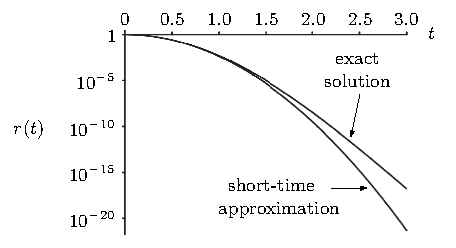
\includegraphics[width=.68\linewidth]{figures/ch05_fig05.pdf}
\caption{デコヒーレンス因子$r(t)=\langle E_-(t)|E_+(t)\rangle$、すなわち環境の相対状態の重なりの時間発展。$N=20$個の調和振動子からなる環境について、厳密な発展(5.108)と短時間近似(5.110)の両方を示した。結合$g_i$と振動数$\omega_i$は、区間$[0,1]$から無作為に選んだ。}\label{fig:5.5}
\end{figure}

% 原文 p.214
\hypertarget{srcpage:214}{}\label{srcpage:214}
系の縮約密度行列$\rho_{\mathrm S}(t)$の時間発展は、通常の方法で
\chfiveeq{114}
から得られる。$\hat V(t)$は(5.99)で与えられる。$\{|0\rangle,|1\rangle\}$基底で表した$\hat\rho_{\mathrm S}(t)$の対角要素$\rho_{\mathrm S}^{(ii)}(t)$が時間に対して一定、
\chfiveeq{115}
であることは(5.92)からすでにわかっているので、非対角要素
\chfiveeq{116}
だけを計算すればよい。上の定義を用いれば、これらは次のように容易に計算できる。
\chfiveeq{117}
言い換えれば、デコヒーレンス因子$r(t)$は
\chfiveeq{118}
で与えられる。すなわち、環境の熱モード$\hat\rho_{\mathrm E_i}$についての、演算子$\hat D(\lambda_i(t))$［(5.103)参照］の期待値の積である。

ここで
\chfiveeq{119}
は、熱平衡にある一つの調和振動子、すなわち一つの場モードの、対称順序の特性関数にすぎないことがわかる。この関数は量子光学でよく知られ（例えば文献\cite{ref241}）、次で与えられる\cite{ref018,ref150}。
\chfiveeq{120}

% 原文 p.215
\hypertarget{srcpage:215}{}\label{srcpage:215}
よって
\chfiveeq{121}
であり、指数関数の引数を$\Gamma(t)$と表した。

\subsubsectionlink*{デコヒーレンス因子の時間発展}
かなり形式的な操作を行ってきたので、次に$\Gamma(t)$を調べ、$r(t)$の時間依存性の感覚をつかもう。まず、環境が十分大きく、環境モードの連続的な密度を仮定できるとする。したがって、5.2節の量子Brown運動の議論と同様に、離散的結合$g_i$の和で表した(5.121)から、スペクトル密度$J(\omega)$による連続記述へ移る。
\chfiveeq{122}
この置換により、(5.121)の$\Gamma(t)$は
\chfiveeq{123}
となる。もちろん、
\chfiveeq{124}
を選べば、(5.123)の右辺は、自明に元の表式(5.121)と一致する。ここでは代わりに、$J(\omega)$を、適切に選んだ$\omega$の滑らかな関数で表そう。

量子Brown運動の場合（5.2.3節参照）と同様に、十分小さい振動数でOhmic、$J(\omega)\propto\omega$であり、$\Lambda$で定量化する滑らかな高振動数カットオフをもつスペクトル密度を考える。量子Brown運動模型で用いたLorentz--Drude形(5.44)の代わりに、ここでは$e^{-\omega/\Lambda}$という指数関数的なカットオフを選ぼう。したがってスペクトル密度は
\chfiveeq{125}
という形を取る。$J_0$は無次元定数である。(5.123)に現れる因子4を(5.125)へ吸収した。このスペクトル密度を図5.6に示す。意図したとおり、$J(\omega)$は$\omega<\Lambda$でほぼ線形に増加し、$\omega>\Lambda$で減少する。

$J(\omega)$の関数形(5.125)を用いると、(5.123)は
\chfiveeq{126}
となる。

% 原文 p.216
\hypertarget{srcpage:216}{}\label{srcpage:216}
\begin{figure}[htbp]\centering
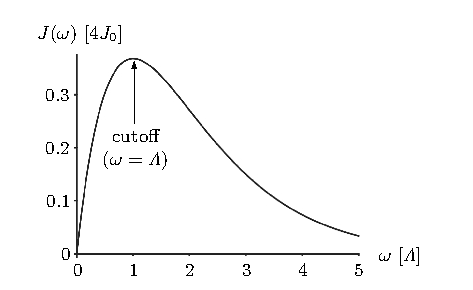
\includegraphics[width=.65\linewidth]{figures/ch05_fig06.pdf}
\caption{(5.125)で与えられるスペクトル密度$J(\omega)$（単位：$4J_0$）。スペクトル密度は、カットオフ振動数$\Lambda$より十分低い振動数では、ほぼOhmic、すなわち$J(\omega)\propto\omega$になるように選んだ。$\omega>\Lambda$では、Ohmicな性質は$e^{-\omega/\Lambda}$という項によって抑えられる。振動数$\omega$の単位はカットオフ$\Lambda$である。}\label{fig:5.6}
\end{figure}
環境の熱エネルギー$k_{\mathrm B}T$がカットオフ振動数$\Lambda$より小さい、$k_{\mathrm B}T\ll\Lambda$という妥当な仮定を置くと、この積分は厳密に解ける。結果は
\chfiveeq{127}
と分解できる。ここで
\chfiveeq{128}
は、純粋に量子的な真空揺らぎによる$\Gamma(t)$への厳密な寄与であり（浴温度に依存しないことに注意）、
\chfiveeq{129}
は、浴の熱揺らぎによる寄与である。

$\Gamma(t)$のグラフを図5.7に示す。$\Gamma(t)$は初期値1から減少する。関係するデコヒーレンス因子(5.118)は$r(t)=e^{\Gamma(t)}$なので、成分$|0\rangle$と$|1\rangle$の間のコヒーレンスは、確かに局所的に減衰すると結論できる。以下で見るように、このデコヒーレンス過程には、いくつかの特徴的な時間尺度を区別できる。

\subsubsectionlink*{デコヒーレンスの時間尺度}
二つの寄与$\Gamma_{\mathrm{fluc}}(t)$、$\Gamma_{\mathrm{therm}}(t)$のいずれかが、$\Gamma(t)$の時間発展を支配する、関係する時間尺度を調べよう。

% 原文 p.217
\hypertarget{srcpage:217}{}\label{srcpage:217}
\begin{figure}[htbp]\centering
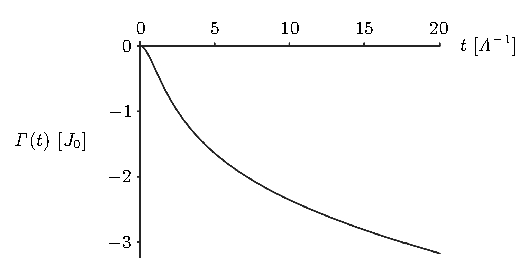
\includegraphics[width=.65\linewidth]{figures/ch05_fig07.pdf}
\caption{指数$\Gamma(t)$［(5.126)参照］の時間依存性（単位：$J_0$）。時間の単位はカットオフ周期$\Lambda^{-1}$である。浴温度は$k_{\mathrm B}T=\Lambda/60$、すなわち熱相関時間がカットオフ周期$\Lambda^{-1}$の60倍長いと仮定した。}\label{fig:5.7}
\end{figure}
(5.128)、(5.129)から、これらの時間尺度は、カットオフ周期$\Lambda^{-1}$と熱相関時間$(k_{\mathrm B}T)^{-1}$に対する$t$の大きさによって定義されるとわかる。

第一に、$t\ll\Lambda^{-1}$かつ$t\ll(k_{\mathrm B}T)^{-1}$という、極端に短い時間の領域を仮定しよう。このとき、$\Gamma_{\mathrm{fluc}}(t)$の表式(5.128)の自然対数のTaylor展開は、第2項までで打ち切れる。すなわち、$\Lambda^2t^2$の1次まで展開して、
\chfiveeq{130}
を得る。したがって$\Gamma_{\mathrm{fluc}}(t)\ll1$である。この領域では熱的寄与$\Gamma_{\mathrm{therm}}(t)$はまったく役割を果たさない。よってデコヒーレンス因子$r(t)$［(5.118)参照］は1に近く、その弱い減衰は、すべて量子的真空揺らぎによる。

第二に、$t$がカットオフ振動数で定まる特徴的周期より大きい、$t\gg\Lambda^{-1}$が、なお熱相関時間よりはるかに小さい、$t\ll(k_{\mathrm B}T)^{-1}$としよう。このときも、$\Gamma(t)$に対する$\Gamma_{\mathrm{therm}}(t)$の寄与を無視でき、$\Gamma_{\mathrm{fluc}}(t)$は
\chfiveeq{131}
と近似できる。したがって、$\Gamma_{\mathrm{fluc}}(t)$の大きさは1より大きく、この領域では量子的真空揺らぎが、支配的なデコヒーレンス源となる。

最後に、$t$が典型的な熱揺らぎ時間よりはるかに大きい長時間領域、$t\gg(k_{\mathrm B}T)^{-1}$を仮定しよう。このとき
\chfiveeq{132}
を用いると、
\chfiveeq{133}
したがって
\chfiveeq{134}
を得る。

% 原文 p.218
\hypertarget{srcpage:218}{}\label{srcpage:218}
この$\Gamma(t)$の表式を(5.121)へ代入すると、デコヒーレンス因子$r(t)$は、熱相関時間$(k_{\mathrm B}T)^{-1}$で定まる時間尺度で指数関数的に減衰することがわかる。
\chfiveeq{135}

% 原文 pp.218--222
\subsubsectionlink{スピン・ボソン模型のBorn--Markovマスター方程式}
前の5.3.1節で論じた、簡単化したスピン・ボソン模型では、全Hamiltonian(5.90)は中心スピンの$\hat\sigma_z$固有基底で完全に対角的だった。これは、スピン系が$\{|0\rangle,|1\rangle\}$基底で固有の運動をもたないことを意味する。系が環境に結合していなければ、測定で系を$|0\rangle$または$|1\rangle$に見いだす確率は、時間とともに変化しない。

次に、Hamiltonian(5.90)へトンネル項$-\Delta_0\hat\sigma_x/2$を加え、固有の運動を含むように、この模型を一般化しよう。$\Delta_0$はトンネル行列要素である［(5.1)参照］。環境座標を$(\hat q_i,\hat p_i)$表示に戻すと、一般的なスピン・ボソン模型はHamiltonian
\chfiveeq{136}
で定義される。Leggettら\cite{ref209}は、このHamiltonianの形を物理的考察から厳密に動機づける方法を、詳しく示している。ここでの目的には、スピン系と振動子環境の模型の役割についての5.1節の導入的な説明で、Hamiltonian(5.136)への関心を動機づけるには十分であるとする。

このHamiltonianは、5.3.1節で考えたトンネル効果のないHamiltonian(5.90)より、わずかに複雑になっただけのように見える。それにもかかわらず、トンネル項の存在によって、(5.136)で定義する一般的スピン・ボソン模型は、数学的解法の点でも、得られるデコヒーレンスの動力学の、パラメータの相対的大きさへの依存性の点でも、はるかに複雑になる。前述のLeggettらの総説\cite{ref209}は、この模型の厳密解と近似解を、非常に詳しく論じている。

ここでは、スピン・ボソン模型のBorn--Markovマスター方程式の導出に注目する。系が大きな環境に弱く結合する場合、このマスター方程式が適切であることを思い出そう。以下の計算を容易にするため、Hamiltonian(5.136)に、小さな簡単化を一つ導入する。

% 原文 p.219
\hypertarget{srcpage:219}{}\label{srcpage:219}
すなわち、中心系が対称な二重井戸ポテンシャルを運動する場合に対応して、非対称エネルギー$\omega_0$がゼロであると仮定する。この仮定により、(5.136)の最初の$\hat\sigma_z$の項が消え、模型はHamiltonian
\chfiveeq{137}
で定義される。この、(5.136)をわずかに簡単化したHamiltonianの形によって、Born--Markovマスター方程式の導出が見通しよくなり、量子Brown運動との興味深い類似性も、より明確に確立できる。

幸い、導出は量子Brown運動の場合（5.2.1節参照）と非常に似た方法で進められる。実際、同じ種類の環境と、双線形の系・環境結合を扱うので、多くの結果をそのまま引き継げる。例えば、量子Brown運動のマスター方程式の導出の大部分は、環境自己相関関数(5.15)の計算に費やされた。これらの関数は中心系の表現に依存しないので、以下では、5.2.1節で得た結果を直接用いられる。

特に、量子Brown運動のマスター方程式の形(5.22)を引き継ぎ、位置演算子$\hat X$をPauliの$z$スピン演算子$\hat\sigma_z$に置き換えるだけでよい。
\chfiveeq{138}
ここで$\hat H_{\mathrm S}=-\Delta_0\hat\sigma_x/2$は系のHamiltonianである。(5.138)の雑音核$\nu(\tau)$と散逸核$\eta(\tau)$は、量子Brown運動の場合とまったく同じ形(5.16)、(5.17)、すなわち
\chfiveeq{139_140}
を取る。相互作用描像での演算子$\hat\sigma_z$の時間依存性は、系のHamiltonian $\hat H_{\mathrm S}$についてのHeisenberg運動方程式を解けば計算できる。結果は
\chfiveeq{141}
である。

% 原文 p.220
\hypertarget{srcpage:220}{}\label{srcpage:220}
この表式が、量子Brown運動模型で用いた相互作用描像の位置演算子$\hat X(\tau)$の結果(5.24)と、形式的に似ていることに注意しよう。

(5.141)をマスター方程式(5.138)へ代入する。項を整理し、Pauliスピン演算子の標準的恒等式$\hat\sigma_y\hat\sigma_z=\mathrm i\hat\sigma_x$、$\hat\sigma_z\hat\sigma_y=-\mathrm i\hat\sigma_x$を用いる、直接的な代数計算の後、Hamiltonian(5.137)で定義するスピン・ボソン模型のBorn--Markovマスター方程式の最終形
\chfiveeq{142}
を得る。

この方程式には、いくつかの新しい量が現れる。まず
\chfiveeq{143}
は、系の繰り込まれた、一般には非HermiteのHamiltonianである。すなわち、トンネル項$-\Delta_0/2$は、環境の影響によって$\zeta^*$だけ変わり、
\chfiveeq{144}
である。(5.142)、(5.144)に現れる係数$\widetilde D$、$\widetilde f$、$\widetilde\gamma$は、量子Brown運動模型の通常拡散係数$D$、異常拡散係数$f$［(5.26c)、(5.26d)参照］、減衰係数$\gamma$［(5.26b)参照］に、それぞれ類似した表式
\chfiveeq{145a_145b_145c}
で決まる。したがって、環境のスペクトル密度の具体形を選べば、係数(5.145)は、量子Brown運動の場合（5.2.3節参照）とほぼ同じ方法で評価できる。

マスター方程式(5.142)の右辺の各項の解釈も、量子Brown運動の場合と似ている。項
\chfiveeq{146}
は、標準のLindblad二重交換子の形(4.45)である。

% 原文 p.221
\hypertarget{srcpage:221}{}\label{srcpage:221}
相互作用Hamiltonianの構造［(5.136)参照］からすでに明らかなように、これは、環境による系の観測量$\hat\sigma_z$の直接監視を表す。したがって、係数$\widetilde D$で与えられる率での、基底$\{|0\rangle,|1\rangle\}$のデコヒーレンスを記述する。

このことは、(5.146)を$\{|0\rangle,|1\rangle\}$基底の$2\times2$行列として表しても、具体的に見られる。縮約密度行列の要素$\langle i|\hat\rho_{\mathrm S}(t)|j\rangle$、$i\in\{0,1\}$を$\rho_{\mathrm S}^{(ij)}(t)$と書けば、
\chfiveeq{147}
を得る。したがって、マスター方程式の他のすべての項を無視し、$\widetilde D$の項(5.146)だけによる、$\hat\sigma_z$固有基底での縮約密度行列の非対角要素の時間発展は
\chfiveeq{148}
である。これは、率$\widetilde D$での非対角要素の指数関数的減衰を意味する。対角要素$\rho_{\mathrm S}^{(00)}(t)$、$\rho_{\mathrm S}^{(11)}(t)$、すなわち占有確率は、項(5.146)が生成する運動の影響を受けず、減衰を伴わない純粋なデコヒーレンス過程であることを示す。このことも、通常拡散項が空間的コヒーレンスを指数関数的に減衰させた、量子Brown運動の場合［(5.35)参照］に類似している。

トンネル行列要素が消える$\Delta_0=0$の場合、$\zeta=0$でもあることに注意しよう。このときマスター方程式(5.142)は、減衰や振動数シフトに対応する項を含まない「純粋デコヒーレンス」の形
\chfiveeq{149}
に帰着する。これは、Lindblad演算子$\hat L=\hat\sigma_z$をもつLindblad方程式(4.45)にすぎず、環境による系の$z$スピン値の監視を記述する。

最後に、マスター方程式(5.142)の右辺の最後の二項は、係数$\widetilde f$、$\widetilde\gamma$［(5.145b)、(5.145c)参照］の兼ね合いで定量化される、二準位系の崩壊を記述する。これは、例えば各項を行列形で書き下せば、かなり容易にわかる（ここではデコヒーレンスに注目するため、証明は示さない）。

% 原文 p.222
\hypertarget{srcpage:222}{}\label{srcpage:222}
まとめると、スピン・ボソン模型のBorn--Markovマスター方程式は、量子Brown運動のマスター方程式の導出と、非常に類似した方法で得られることがわかった。次の段階は、Born--Markov近似を超えて、スピン・ボソン模型を調べることである。この近似は、中心二準位系と環境が非常に低温にある物理的状況では、しばしば破れる（4.4節の議論参照）。そのような低温系の顕著な例は、絶対零度に近い温度で動作する超伝導量子ビット系である（6.3節参照）。

前述のように、スピン・ボソン模型の豊かな非Markov動力学は、Leggettら\cite{ref209}が非常に詳しく解析している。予想どおり、その運動は、環境温度、スペクトル密度の形（subohmic、Ohmic、supraohmic）、系と環境の全体的結合強度など、模型のさまざまなパラメータに強く依存する。それぞれのパラメータ領域には、局在化、指数関数的または非コヒーレントな緩和、指数関数的減衰、強くまたは弱く減衰したコヒーレント振動という、特徴的な運動が現れる（パラメータ領域と対応する動力学の概観は、文献\cite{ref209}の表I参照）。

ここでは、このかなり複雑な動力学は論じず、上で調べた二つの模型、すなわち簡単化したスピン・ボソン模型と、Born--Markov近似の枠組みでのスピン・ボソン模型で満足することにしよう。これらの模型は、スピン・ボソン型模型のデコヒーレンス研究に関係する主要な特徴を、すでに示している。スピン・ボソン模型の散逸とデコヒーレンスの非Markov動力学を深く解析したい読者は、Leggettらの論文\cite{ref209}とWeissの著書\cite{ref218}に、膨大な情報を見いだすだろう。

% 原文 p.222

\subsectionlink{スピン環境模型}
それでは、調和振動子からなる環境の研究から、環境をスピン$1/2$粒子、すなわち量子二準位系の集合で表す模型の分析へ、焦点を移そう。5.1.2節では、そのようなスピン環境を考える物理的動機と、振動子環境との主要な違いを、すでに論じた。

スピン粒子で表された中心系が、ほかのスピンの集まりに線形に結合する系は、物理的に最も重要で、最もよく研究されたスピン環境模型である。この「スピン・スピン模型」が適する典型的状況は、超伝導量子ビットなどの単一の二準位系が、低温環境に強く結合する場合である（5.1節の議論参照）。もう一つの「標準的」可能性である、
% 原文 p.223
\hypertarget{srcpage:223}{}\label{srcpage:223}
中心調和振動子と二準位系環境との相互作用は、いわゆる量子電気機械系（6.4.2節参照）や、$\mu\mathrm m$尺度のイオントラップ\cite{ref242}でのデコヒーレンスと散逸の研究において、最近ようやく注目され始めた。

本節では、そのようなスピン環境模型の異なる側面を調べる。スピン・スピン模型の議論は、スピン・ボソン模型と同じような構成とする。まず5.4.1節では、2.10節のデコヒーレンス模型を単純に一般化した、スピン・スピン模型を論じる。次の5.4.2節では、系と環境の線形結合が弱い極限の、スピン環境模型を論じる。この場合には、FeynmanとVernon\cite{ref211}が最初に示唆したように、修正したスペクトル密度を持つ振動子環境へ、スピン環境を写像できることを示す（5.1.2節も参照）。これにより、量子Brown運動の研究から得た形式的結果を引き継ぎ、スピン浴と弱く相互作用する中心系について、(5.22)の形のBorn--Markovマスター方程式を導ける。

5.4.3節では、より一般的なスピン・スピン模型の特徴を論じる。解くための数学には立ち入らず、そのような模型に生じるデコヒーレンス動力学の概観に重点を置く。スピン環境模型の理論を、より詳しく知りたい読者には、Prokof'evとStampの総説\cite{ref199}に豊富な内容がある。短く分かりやすい要約は\cite{ref200}にある。

\subsubsectionlink{単純な動力学的スピン・スピン模型}
2.10節で、環境デコヒーレンスと超選択の基本的特徴を示す原型的模型を論じた際、スピン・スピン模型の一つに、すでに出会っている。中心スピンとスピン環境の自己Hamiltonianを両方とも無視し、相互作用Hamiltonianが、中心スピンと環境スピン集合の両方の$\hat\sigma_z$固有基底ですでに対角であると仮定したため［(2.100)参照］、全体の動力学を容易に厳密に解けた。この模型は明らかに、かなり人工的であった。系と環境の内部動力学を模型化せず、動力学を完全に支配する強い系・環境相互作用の極限、すなわち量子測定領域に対応していたからである。

ここでは、元のHamiltonian(2.100)へ$-\frac12\Delta_0\hat\sigma_x$の形のトンネル項［(5.1)参照］を加え、この静的スピン・スピン模型を一般化する。すなわち、全Hamiltonian
\chfiveeq{150}
で記述される模型を考える。(5.150)へトンネル項を含めると一般に、Hamiltonian(2.100)で定義される元の静的模型とは、著しく異なる動力学になることを示す。
% 原文 p.224
\hypertarget{srcpage:224}{}\label{srcpage:224}
(5.150)右辺の最後の項は、中心系の$z$スピン座標と、各環境スピンの$z$スピン座標との、おなじみの線形相互作用に対応し、結合強度は$g_i$である。

\paragraphlink{模型を解く}
トンネル項があっても、(5.150)の模型の全体の動力学は、Dobrovitskiら\cite{ref243}およびCucchietti、Paz、Zurek\cite{ref118}が示したように、厳密に解ける。以下の導出では、後者の方法\cite{ref118}に詳しく従う。

Hamiltonian(5.150)を簡単にする主要な特徴は、静的な場合(2.100)と同じく、環境演算子として$\hat\sigma_z$だけを含むことである。したがって、2.10節の模型と同様、Hamiltonianの環境部分$\hat E$の固有状態$|n\rangle$は、第$i$環境演算子$\hat\sigma_z^{(i)}$の固有状態$|\uparrow\rangle_i$、$|\downarrow\rangle_i$の積で与えられる［(2.101)参照］。明示的には、
\chfiveeq{151}
で、固有値は［(2.102)参照］、
\chfiveeq{152}
である。第$i$環境スピンが「上」なら$n_i=0$、「下」なら$n_i=1$である。

ここで、純粋な系・環境積状態
\chfiveeq{153}
を考える。$|\psi_{\mathrm S}\rangle$は、系の任意の状態ベクトルである。この状態へのHamiltonian(5.150)の作用は、
\chfiveeq{154}
となる。すなわち、各環境状態$|n\rangle$について、対応する有効系Hamiltonian
\chfiveeq{155}
を考えられる。任意の初期積状態
\chfiveeq{156}
% 原文 p.225
\hypertarget{srcpage:225}{}\label{srcpage:225}
の時間発展は、
\chfiveeq{157}
と書け、したがって、
\chfiveeq{158}
となる。ここで$\hat\rho_{\mathrm S}(0)=|\psi_{\mathrm S}(0)\rangle\langle\psi_{\mathrm S}(0)|$である。$\hat U_n(t)$は、有効Hamiltonian(5.155)に対応する系の発展演算子で、次で与えられる\cite{ref118}。
\chfiveeq{159}
ここで$\Omega_n=\sqrt{\epsilon_n^2+\Delta_0^2/4}$である。

\cite{ref118}に従い、縮約密度行列$\hat\rho_{\mathrm S}(t)$を、いわゆる偏極ベクトル$\boldsymbol p(t)\equiv(p_x(t),p_y(t),p_z(t))$で、形式的に表そう。
\chfiveeq{160}
$\boldsymbol p$は、次のように解釈できる。大まかには、その向きが、密度行列(5.160)がどの固有状態の組に分解されるかを教える。たとえば$p_x=p_y=0$なら、
\chfiveeq{161}
であり、固有状態は$\hat\sigma_z$の固有状態$|0\rangle$、$|1\rangle$となる。他方、$p_y=p_z=0$なら、
\chfiveeq{162}
となり、固有状態は$\hat\sigma_x$の固有状態である。

偏極ベクトル$\boldsymbol p(t\to\infty)$の支配的成分は、デコヒーレンス過程がどの「向き」、すなわちどの基底で最も有効かを教える。したがって、偏極ベクトルによる記述は、この模型に現れる優先的指針基底を、直観的に分析できる。たとえば$p_x(t)$、$p_y(t)$がゼロへ向かい、$p_z(t)$が有限の漸近値へ近づけば、$\hat\sigma_z$の固有基底$\{|0\rangle,|1\rangle\}$が系の指針基底だと結論できる。

次の目標は、縮約密度行列(5.158)に対応する偏極ベクトルの成分$p_x(t)$、$p_y(t)$、$p_z(t)$を計算することである。
% 原文 p.226
\hypertarget{srcpage:226}{}\label{srcpage:226}
これにより、得られる系の動力学を調べられる。右辺の和の各項$\hat U_n(t)\hat\rho_{\mathrm S}(0)\hat U_n^\dagger(t)$に対応する明示的な式$(p_x^{(n)}(t),p_y^{(n)}(t),p_z^{(n)}(t))$は、$\hat U_n(t)$の具体的表式(5.159)を使えば、かなり容易に得られる。結果は\cite{ref118}を参照されたい。

次に、$s\in\{x,y,z\}$に対する$|c_n|^2p_s^{(n)}(t)$という個々の項をすべて足し、全偏極ベクトルを得る［(5.158)、(5.160)参照］。離散添字$n$を使う代わりに、通常の方法に従い、(5.158)を等価な積分形へ書き換えよう。
\chfiveeq{163}
ここでは、環境エネルギー$\epsilon$の分布を記述するスペクトル密度を導入した。
\chfiveeq{164}
Cucchietti、Paz、Zurek\cite{ref118}が示したように、環境スピンの数$N$が大きいと、この分布はGauss分布へ近づく。
\chfiveeq{165}
Gauss分布(5.165)の幅$s_N$は、環境エネルギー$\epsilon$の典型的範囲を定量化する［(5.152)参照］。2.10節では、すべての環境結合と展開係数が等しいという、簡単化した状況で、この結果を証明した。しかし(5.165)は、はるかに一般的な係数の選択でも成り立ち、$N$がすでにかなり小さい場合でも、厳密な式(5.164)のよい連続体近似となる\cite{ref118}。

Gauss型スペクトル密度(5.165)を使うと、偏極ベクトルの三成分は次となる\cite{ref118}。
\chfiveeq{166a_166b_166c}
ここで$\Omega=\sqrt{\epsilon^2+\Delta_0^2/4}$である。

% 原文 p.227
\hypertarget{srcpage:227}{}\label{srcpage:227}
\paragraphlink{模型の動力学}
上の積分(5.166)を、二つの重要な極限で評価しよう。第一の$\Delta_0\ll s_N$は、系の固有動力学が弱い場合に対応する。この極限では、系の自己Hamiltonianの存在は、動力学にほとんど影響しない。したがって、2.10節の静的模型の結果へ近づくと予想する。Cucchietti、Paz、Zurek\cite{ref118}の研究に従い、この場合の偏極ベクトルの成分(5.166)の発展を、図5.8上に示す。初期偏極は、演算子$\hat\sigma_x$、$\hat\sigma_y$、$\hat\sigma_z$のいずれの固有状態にも偏らないように、$p_x(0)=p_y(0)=p_z(0)=1/\sqrt3$とした。

$p_x(t)$、$p_y(t)$は初期値から急速に減衰する。$p_y(t)$はゼロへ収束し、$p_x(t)$はゼロに近い正の定数へ近づく。対照的に、$p_z(t)$はほとんど減衰せず、初期値の近くにとどまる。
\begin{figure}[htbp]\centering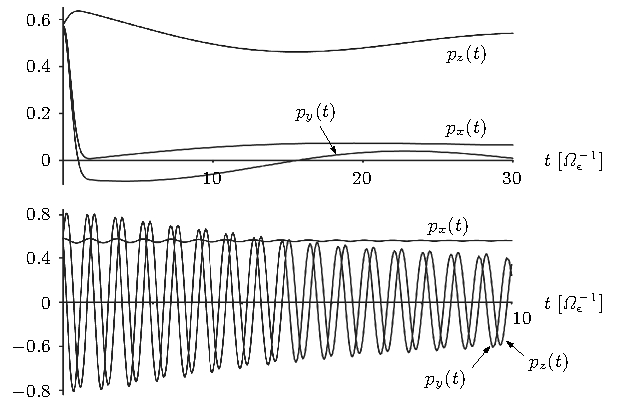
\includegraphics[width=.94\linewidth]{figures/ch05_fig08.pdf}
\caption{Cucchietti、Paz、Zurek\cite{ref118}が調べた、偏極ベクトルの成分$p_x(t)$、$p_y(t)$、$p_z(t)$［(5.166)参照］の時間依存性。このベクトルは、Hamiltonian(5.150)で定義されるスピン・スピン模型の、縮約密度行列の発展［(5.160)参照］を記述する。時間$t$の単位は、系の固有発展の特徴的時間尺度$\Omega_\epsilon^{-1}$である。上は固有動力学が弱い場合（$\Delta_0=0.1s_N$）で、$\hat\sigma_z$の近似的固有状態を優先基底として選ぶ。下は、系の自己動力学が強く、環境モードが低エネルギー、すなわち「遅い」という、逆の状況（$\Delta_0=5s_N$）である。このとき$\hat\sigma_x$、したがって自己Hamiltonianの、近似的固有状態が指針状態として現れる。}
\end{figure}
% 原文 p.228
\hypertarget{srcpage:228}{}\label{srcpage:228}
成分$p_x(t)$と$p_z(t)$の最終値の比は、小さい比$\Delta_0/s_N$と同程度となる。したがって、環境が選ぶ優先的指針状態は、$\hat\sigma_x$からの小さな寄与を伴う、$\hat\sigma_z$固有状態に近いことが分かる。

第二の極限、環境が利用できる最大エネルギーが系のエネルギー間隔$\Delta_0$より小さい、$s_N\ll\Delta_0$の場合を考えよう。対応する偏極成分の発展を図5.8下に示す。$p_y(t)$、$p_z(t)$は、包絡線が急速に減衰する振動を示し、$p_x(t)$は$1/2$に近い定常値へ速やかに落ち着く。このことは、動力学的に選ばれる優先基底が、今度は$x$スピン演算子$\hat\sigma_x$、したがって自己Hamiltonianの固有基底に近いことを意味する。すなわち、動力学は、エネルギー固有状態を系の指針基底として選ぶ。

この模型は、系の自己Hamiltonianと相互作用Hamiltonianの相対的強さに、優先基底が依存することを、よく示す。優先基底は、全Hamiltonianの下で最も頑健な局所基底として現れる。見たように、相互作用Hamiltonianが自己Hamiltonianを支配する量子測定極限、$\Delta_0\ll s_N$では、優先状態は相互作用Hamiltonianの固有状態となり、2.8.1節の可換性基準(2.89)に一致する。逆に、環境モードが「遅く」、$s_N\ll\Delta_0$で、自己Hamiltonianが系の発展を支配すると、優先基底は「局所的」エネルギー固有状態、すなわち自己Hamiltonianの固有状態で与えられる。2.8.2節で強調したように、このデコヒーレンスの量子極限\cite{ref103}は、環境の存在を単に無視することとは等価でない。むしろ、環境はエネルギー固有状態の重ね合わせをデコヒーレンスさせる。

\subsubsectionlink{弱結合極限のスピン環境模型：振動子環境への写像}
系と環境の結合が弱いという仮定の下では、ある環境と相互作用する縮約系の動力学を、等価な調和振動子環境とその系との相互作用として表せる、という注目すべき事実に、すでに各所で触れた\cite{ref211,ref212}。スピン環境の写像を最初に調べたのは、Caldeira、Castro Neto、de Carvalho\cite{ref208}である。

この写像は、振動子環境によって生じる系の動力学が、スピン環境によるものと同一になる、という意味ではないことを強調する。実際、得られる動力学は一般に大きく異なる。むしろ「写像」で伝えたいのは、あるスペクトル密度のスピン環境中での縮約動力学が、元のスピン環境のスペクトル密度を適切に修正したものによって記述される、振動子環境中での縮約動力学と、同一であるという知見である。言い換えれば、
% 原文 p.229
\hypertarget{srcpage:229}{}\label{srcpage:229}
スピン環境のBorn--Markovマスター方程式は、振動子環境のBorn--Markovマスター方程式(5.22)を、修正したスペクトル密度で評価して与えられる。その方法を示そう。

\paragraphlink{模型}
スピン環境模型のHamiltonianを、通常の形に分解する。
\chfiveeq{167}
ここで$\hat H_{\mathrm S}$は、系の一般的な自己Hamiltonianである。環境の自己Hamiltonianも含めた。
\chfiveeq{168}
$\Delta_i$は、第$i$環境スピンのトンネル行列要素である。この自己Hamiltonianは、2.10節と5.4.1節の、より単純なスピン環境模型とは異なり、環境に固有の動力学を与える。簡単のため、各スピンの非対称エネルギーはゼロ、すなわち各環境「粒子」が対称二重井戸ポテンシャル中を動くとする\footnote{非対称エネルギーが非ゼロで、したがって自己Hamiltonian(5.168)に$\hat\sigma_z^{(i)}$に比例する項が含まれる場合も、本節とほぼ同じ方法で扱える\cite{ref242}。}。

最後に、相互作用Hamiltonian$\hat H_{\mathrm{int}}$は通常の形となる［(5.150)と比較］。
\chfiveeq{169}
すなわち、系の一般的座標$\hat s$が、各環境スピンへ双線形に結合し、強度は$g_i$で定量化される。後で、スピン系の$\hat s=\hat\sigma_z$、すなわち「スピン・スピン模型」と、調和振動子系の$\hat s=\hat X$の場合に、特化する。

\paragraphlink{スピン環境の自己相関関数の計算}
弱い系・環境結合の極限を仮定し、環境は温度$T$で熱平衡にあるとする。このスピン浴模型のBorn--Markovマスター方程式（4.2節参照）を導きたい。まず目標となるのは、環境自己相関関数(4.10)の導出である。量子Brown運動の場合［(5.5)と比較］と同じく、相互作用Hamiltonian(5.169)は一項だけを含むので、計算すべき環境自己相関関数は、ただ一つである。
\chfiveeq{170}
% 原文 p.230
\hypertarget{srcpage:230}{}\label{srcpage:230}
ここで$\hat E(\tau)=e^{i\hat H_{\mathrm E}\tau}\hat E e^{-i\hat H_{\mathrm E}\tau}$は、(5.169)で定義した集団的環境演算子$\hat E$を、相互作用描像で表したものである。

環境スピン同士は相互作用せず、したがって$i\ne j$で$[\hat\sigma_x^{(i)},\hat\sigma_z^{(j)}]=0$なので、指数関数$e^{i\hat H_{\mathrm E}\tau}$は、単一スピンの項へ因数分解される。
\chfiveeq{171}
したがって、環境自己相関関数(5.170)は、次と書ける。
\chfiveeq{172}
ここで再び、環境スピンが直接相互作用せず、したがって無相関である事実を使うと、$i\ne j$について、
\chfiveeq{173}
となる。量子Brown運動模型での同様の議論については、(5.7)を比較されたい。したがって、(5.172)の和を分解できる。
\chfiveeq{174}
次に、スピン浴による「量子的力」の平均が$t=0$でゼロ、すなわち、
\chfiveeq{175}
と仮定する。もしゼロでなくても、定数を加えれば常に実現できるので、制限を課す仮定ではない。このことは、(5.174)右辺の最初の和に現れる項$\sum_{j\ne i}g_j\langle\hat\sigma_z^{(j)}\rangle_{\hat\rho_{\mathrm E}}$も、近似的にゼロであることを意味する。これにより$i\ne j$の交差項を無視し、(5.172)を大幅に簡単化できる。
\chfiveeq{176}
最後の行では、浴の初期状態$\hat\rho_{\mathrm E}$についての熱平均を、$Z=\operatorname{Tr}_{\mathrm E}e^{-\hat H_{\mathrm E}/(k_{\mathrm B}T)}$として、明示的に書いた。まず、浴スピンが無相関なので、すべてのスピンを含む初期状態の熱平均は、単一スピンの平均に還元される。
% 原文 p.231
\hypertarget{srcpage:231}{}\label{srcpage:231}
\chfiveeq{177}
ここで$Z_i$は(5.112)と同じ定義である。次に、相互作用描像の演算子$\hat\sigma_z^{(i)}(\tau)$の時間発展を計算する必要がある。
\chfiveeq{178}
$\hat\sigma_z^{(i)}$の固有基底を$\{|\uparrow\rangle_i,|\downarrow\rangle_i\}$とすると、環境Hamiltonian$\hat H_{\mathrm E}^{(i)}$の明示的行列表現は、
\chfiveeq{179}
である。対角化により、固有値$E_\pm=\pm(-\Delta_i/2)$と、固有ベクトル$|\pm\rangle_i=(|\uparrow\rangle_i\mp|\downarrow\rangle_i)/\sqrt2$が得られる。新しい基底$\{|+\rangle_i,|-\rangle_i\}$では、演算子$\hat\sigma_z^{(i)}$は、
\chfiveeq{180}
という形となる。したがって、相互作用描像の時間発展は、
\chfiveeq{181}
である。これらの具体的表式を使うと、(5.177)右辺の波括弧内は、
\chfiveeq{182}
となる。この式のトレースを、簡単のため$\{|+\rangle_i,|-\rangle_i\}$基底で取り、
\chfiveeq{183}
を用いると、環境自己相関関数(5.177)の具体的形が得られる。
\chfiveeq{184}
最後に、通常の手順に従って、環境自己エネルギー$\Delta_i$についての離散和を、スペクトル密度
% 原文 p.232
\hypertarget{srcpage:232}{}\label{srcpage:232}
\chfiveeq{185}
を用いて積分へ置き換える。環境自己相関関数の最終表式が得られる。
\chfiveeq{186}
これが主要な結果である。スピン浴が等価な振動子浴へどう写像されるかを見るため、これを使おう。

\paragraphlink{スピンから振動子への写像}
スピン環境自己相関関数の式(5.186)を、調和振動子浴の場合に得た環境自己相関関数(5.15)、すなわち、
\chfiveeq{187}
と比較しよう。ここで、
\chfiveeq{188}
は、調和振動子環境のスペクトル密度である。スピン浴の場合の対応物と区別するため、添字「osc」を付けた。

(5.186)と(5.187)を比べると、振動子浴で明示的な温度依存性を持っていた雑音核$\nu(\tau)$、すなわち$C_{\mathrm{osc}}(\tau)$の実部は、スピン浴では、その温度依存性を失っている。式(5.186)の$C(\tau)$の実部は、明示的な温度依存性を含まない。他方、スピン浴の$C(\tau)$の虚部には、温度依存因子$\tanh[\Delta/(2k_{\mathrm B}T)]$があるが、$C_{\mathrm{osc}}(\tau)$の対応する散逸核$\eta(\tau)$には、そのような明示的温度依存性がない。

二表式が一致する唯一の場合は、$T\to0$で$\tanh[\Delta/(2k_{\mathrm B}T)]\to1$、$\coth[\omega/(2k_{\mathrm B}T)]\to1$となる、零温度の場合である。これは次のように理解できる。零温度では、それぞれの環境中のスピンも調和振動子も、実効的に基底状態に閉じ込められ、励起状態を占められない。したがって、スピンは二次元状態空間に限られるのに、振動子は連続的なエネルギー準位を占められるという、両者の特徴的な違いが、$T\to0$で消え、浴は同様に振る舞う。

% 原文 p.233
\hypertarget{srcpage:233}{}\label{srcpage:233}
しかし、少し工夫すれば、有限温度でも、スピン浴の式(5.186)を振動子浴の式(5.187)へ写像できる。新しい有効スペクトル密度$J_{\mathrm{eff}}(\Delta,T)$を、
\chfiveeq{189}
で定義しよう。$J(\Delta)$は元のスピン浴のスペクトル密度(5.185)である。環境自己相関関数(5.187)に現れる振動子浴の$J_{\mathrm{osc}}(\omega)$を、明示的に温度依存するこの式$J_{\mathrm{eff}}(\Delta,T)$へ置き換える。右辺の積分で記法を$\omega\to\Delta$と変えると、
\chfiveeq{190}
を得る。これは、まさにスピン浴の環境自己相関関数(5.186)である。

したがって、5.2節で振動子浴について導いた、以前のすべての結果を、スピン浴へ引き継ぐ簡単な道筋が見つかった。浴のスペクトル密度に依存する振動子浴の式を、修正した「代用」スペクトル密度(5.189)で評価するだけでよい。それは、真のスピン浴のスペクトル密度$J(\Delta)$に、追加の温度・周波数依存因子$\tanh[\Delta/(2k_{\mathrm B}T)]$を掛けたものである。

特に、スピン浴の核$\nu(\tau)$、$\eta(\tau)$は、次で与えられる。
\chfiveeq{191_192}
これは、新しい有効スペクトル密度(5.189)を、(5.16)、(5.17)へ代入したものである。これらの核の式と、振動子浴の対応する式(5.16)、(5.17)との形式的な違いは、一見それほど大きく見えないかもしれない。しかし、縮約動力学への影響は、非常に大きくなり得る。写像の手順を、二つの具体例で調べよう。

\paragraphlink{例1：スピン・スピン模型からスピン・ボソン模型への写像}
中心系を、$\hat\sigma_z$を介してスピン浴へ双線形に結合する、スピン$1/2$粒子で表す場合を考える。
% 原文 p.234
\hypertarget{srcpage:234}{}\label{srcpage:234}
上の写像法によれば、量子Brown運動のマスター方程式の一般表式(5.22)で、$\hat X\to\hat\sigma_z$と代入すれば、Born--Markovマスター方程式を直ちに書き下せる。
\chfiveeq{193}
核$\nu(\tau)$、$\eta(\tau)$は、今やスピン浴の式(5.191)、(5.192)で与えられる。

スピン・ボソン模型の議論（5.3.2節参照）と同じく、系の自己Hamiltonianを$\hat H_{\mathrm S}=-\frac12\Delta_0\hat\sigma_x$とすると、相互作用描像の演算子$\hat\sigma_z(\tau)$の明示的時間発展は、
\chfiveeq{194}
となる。これを(5.193)へ使うと、マスター方程式
\chfiveeq{195}
が得られる。この方程式は、スピン・ボソンのマスター方程式(5.142)と、形式的に同一である。これはもちろん意外ではない。目標は、スピン浴を、等価な振動子浴、すなわちボソン浴へ写すことであった。(5.195)に現れる量の定義は、スピン・ボソンの場合と同じ［(5.143)、(5.144)、(5.145a)参照］だが、核(5.191)、(5.192)で評価する。

\paragraphlink{例2：振動子・スピン模型から量子Brown運動模型への写像}
写像法のもう一つの例として、中心調和振動子がスピン浴へ弱く結合する場合\cite{ref242}を論じよう。この弱結合「振動子・スピン模型」は、6.4.2節で詳しく論じる、量子電気機械系のデコヒーレンスと散逸の模型化へ、応用できる可能性がある。全Hamiltonian
\chfiveeq{196}
で記述される、かなり一般的な振動子・スピン模型を考える。ここで、
\chfiveeq{197}
% 原文 p.235
\hypertarget{srcpage:235}{}\label{srcpage:235}
は、中心系の固有動力学を表す通常の調和振動子Hamiltonianである。環境の自己Hamiltonian$\hat H_{\mathrm E}$は、おなじみの形(5.168)を持つ。相互作用Hamiltonian$\hat H_{\mathrm{int}}$は、中心振動子の位置座標と、各環境スピンの$z$スピン座標との双線形結合を表す。

再び、弱結合極限が適用されると仮定し、スピン浴から振動子浴への写像の方針に従えば、振動子系の縮約動力学を、調和振動子ポテンシャルに閉じ込めた粒子の、量子Brown運動のBorn--Markovマスター方程式(5.25)で、容易に記述できる。
\chfiveeq{198}
周波数シフト$\widetilde\Omega^2$、運動量減衰率$\gamma$、拡散係数$D$、$f$は、量子Brown運動と同じ表式(5.26)で与えられる。ただし、そこに現れる核$\nu(\tau)$、$\eta(\tau)$は、「代用」スピン浴の核(5.191)、(5.192)へ置き換える。

スピン浴のオーム型スペクトル密度の例を考えよう。
\chfiveeq{199}
これは、量子Brown運動の文脈で考えた、オーム型密度(5.44)と形式的に同一である。5.2.3節で詳述した方法に従い、スペクトル密度の具体形を選ぶと、マスター方程式(5.198)の係数を評価できる。

以前と同様、係数$\gamma$、$D$は、それぞれ二重Fourier正弦変換、余弦変換で与えられる。詳細は5.2.3節の議論を参照されたい。したがって、結果の式を容易に書き下せる［(5.46)、(5.48)と比較］。
\chfiveeq{200_201}
オーム型振動子浴とは対照的に、オーム型スピン浴では、運動量減衰係数$\gamma$が明示的に温度依存する。因子$\tanh[\Omega/(2k_{\mathrm B}T)]$、したがって$\gamma$は、温度が高まると減少する。これは一見、かなり直観に反するかもしれない。「暖かい」環境は、系へより強く影響するか、少なくとも「冷たい」環境より弱い減衰を誘起することはない、と予想するからである。
% 原文 p.236
\hypertarget{srcpage:236}{}\label{srcpage:236}

しかし、この減衰係数の温度依存性は、かなり容易に説明できる。振動子浴では、各振動子は無限個のエネルギー準位を持つため、浴が吸収できるエネルギー量に上限がない。対照的に、スピン$1/2$粒子は二準位しか持たないので、温度、したがって系から吸収できるエネルギー量が高まると、スピン浴全体が非常に速く飽和する。量子Brown運動模型の振動子浴の散逸率は温度に依存しない［(5.46)参照］から、スピン浴が系へ散逸的効果を及ぼす能力は、温度の上昇とともに低下しなければならない。実際、(5.200)が予測する減衰率の温度依存性は、フォノン、すなわち振動子モードと二準位系の相互作用によって散逸が起きる\cite{ref245}、ガラスのような物理系で実験的に観測されている\cite{ref244}。

オーム型スピン浴では、通常拡散係数(5.201)、したがって空間的デコヒーレンス率は、明示的な温度依存性を持たない。これは、$\coth[\Omega/(2k_{\mathrm B}T)]$に従い、環境温度が高いほど空間的デコヒーレンスが強まる、量子Brown運動の通常拡散係数(5.48)と対照的である。実際、Caldeira--Leggett模型の高温極限では、$D$が温度に線形に増すことが分かった［(5.51)参照］。

この違いもまた、各環境粒子が利用できる状態空間の大きさから理解できる。温度とともに、環境振動子が、ますます高く励起された多くの準位を占められることは、環境中の特徴的波長が、ますます短くなることにつながる。典型的環境波長が短いほど、中心系の位置をよく分解でき、得られる経路情報が増すため、空間的デコヒーレンスが強くなる（5.2.6節の議論も参照）。

これに対して、スピン$1/2$粒子が占められるのは二準位だけである。典型的環境波長の範囲、したがって空間的デコヒーレンス率は、温度を高めると非常に速く飽和する。この特定の模型では、それは完全に温度に依存しない率さえもたらす。実際、この模型では環境二準位系が対称二重井戸ポテンシャル中を動くと仮定した。したがって、対応するスピン粒子の二状態は同じエネルギーに結びつけられ、状態空間をさらに制限する。この対称性の仮定を捨て、浴Hamiltonianへ$\sum_i(\omega_i/2)\hat\sigma_z^{(i)}$という非対称項を含めると、空間的デコヒーレンス率に、定数ではあるが、依然として温度非依存の値が加わることを、容易に示せる。この増加は、浴粒子が利用できる状態空間が広がったことを反映し、
% 原文 p.237
\hypertarget{srcpage:237}{}\label{srcpage:237}
それは、より短い環境波長の存在に対応する。

\subsubsectionlink{Markov近似を超えて：一般のスピン環境模型を解く}
最後に、制限的なBorn--Markov近似へ頼らずに、より一般的なこの種の模型をどう解けるか、簡単に示して、スピン環境模型の議論を終えよう。5.1.2節で論じたように、この模型で興味深いのは、通常、低温かつ系・環境結合が強い領域である。このとき、環境には有意な非Markov記憶効果が生じ、簡単化する弱結合近似は通常使えなくなる。したがって、前の5.4.2節で行ったような、弱結合と無視できる環境自己相関時間を基礎に導かれる、近似的なBorn--Markovマスター方程式で扱えないことが多い。そのため、このような非Markovスピン環境模型の数学的解法は、しばしばやや複雑になる。

多くの場合、一般的なスピン環境模型から生じる、たとえば中心スピンの期待値$\langle\hat\sigma_z(t)\rangle$に関する、関係するデコヒーレンス動力学は、インスタントン形式\cite{ref199}などの高度な手法で解析的に計算できる。このとき、強く結合したスピン環境の自由度を、どう適切に「平均」するかが問題となる。Prokof'evとStamp\cite{ref199}は、一般的模型を四つの極限へ分けることで、これを容易にできることを示した。各極限は異なるパラメーター領域を重視し、全Hamiltonianの一般表式の特定の項を捨てる。それぞれを別々に解くと、模型のある量についての平均積分の式が得られる。\cite{ref199}で示されたように、一般の場合にスピン環境を平均し、したがって中心系の縮約動力学を得る正しい手順は、これら四つの別々の平均を、組み合わせて適用するだけで与えられる。ここでは詳細には立ち入らず、関心のある読者には\cite{ref199}を案内する。スピン環境模型の物理的・数学的基礎についての、さらなる議論は、\cite{ref200,ref210,ref214,ref216}にある。

% 原文 pp.237--241
% 原文 p.237

\subsectionlink{まとめ}
デコヒーレンス模型についての本章は、やや長く、技術的になった。そこで主要な結果を、いくつかまとめよう。

% 原文 p.238
\hypertarget{srcpage:238}{}\label{srcpage:238}
\subsubsectionlink*{標準模型への写像}
関心のある物理系の広いクラスは、スピン$1/2$粒子（状態空間が実効的に異なる二つの基底状態に縮約される系の場合）、または、位置と運動量という連続的な正準座標で記述され、あるポテンシャルの中を運動する粒子の、いずれかで表せる。

環境は、非局在化したボソン場モードの準連続体に対応する調和振動子の集まりとして、あるいはスピンで表す局在モードの集まりとして、模型化できる。スピン環境は、中心系に強く結合する低温環境の、適切な模型となる場合が多い。

\subsubsectionlink*{量子Brown運動}
これは、中心粒子が実空間のあるポテンシャルの中を運動し、互いに相互作用しない調和振動子の環境と双線形に相互作用する模型である。中心系を調和振動子で表す場合に注目した。

この模型のBorn--Markovマスター方程式を導いた［(5.25)参照］。
\chfiveeq{202}
右辺の第1項は、$\widetilde\Omega^2$で定量化する振動数シフトを伴うユニタリーな運動を記述する。第2項は、$\gamma$に比例する率での運動量減衰に対応する。第3項は、距離$\Delta X$にわたる空間的コヒーレンスの、率$D(\Delta X)^2$でのデコヒーレンスを記述する。第4項もデコヒーレンスを表すが、特に高温では、しばしば無視できる。マスター方程式(5.202)に現れるすべての係数は、環境の物理的特徴をまとめた、環境スペクトル密度に強く依存する。

高温極限では、多くの場合、中心系の縮約された運動は、Caldeira--Leggettマスター方程式として知られる、(5.202)を簡単化した形でよく近似される。その形は［(5.57)参照］
\chfiveeq{203}
である。ここでも右辺の第1項は、環境によって繰り込まれた自己Hamiltonian $\hat H'_{\mathrm S}$が支配するユニタリーな発展を表し、第2項は散逸を記述し、第3項は、浴の温度に線形に増加する率での、空間的重ね合わせのデコヒーレンスに対応する。

% 原文 p.239
\hypertarget{srcpage:239}{}\label{srcpage:239}
Caldeira--Leggettマスター方程式(5.57)の導出に入った仮定をまとめよう。
\begin{itemize}
\item Born--Markov近似が成り立つ（4.2.1節参照）。
\item 調和振動子の環境は、高振動数カットオフ$\Lambda$をもつOhmicなスペクトル密度$J(\omega)\propto\omega$で記述される。
\item 環境は十分高温であり、その熱エネルギーは系の固有振動数で定まるエネルギー尺度より、はるかに大きい（$k_{\mathrm B}T\gg\Omega$）。
\item 系の固有振動数は、環境の高振動数カットオフ$\Lambda$より、はるかに小さい（$\Omega\ll\Lambda$）。
\end{itemize}
環境監視と固有の運動の相互作用により、最小不確定性Gaussianである指針状態が出現することを見いだした。これらは位置と運動量の両方でよく局在し、位相空間の古典的な点を近似する（5.2.6節参照）。この状態は、環境による位置座標の直接監視と、位置座標・運動量座標について対称な自己Hamiltonianをもつ系の固有の運動の、組み合わさった影響に対して最も頑健な、妥協として生じる。固有の運動は、運動量の重ね合わせから空間的重ね合わせを作ることを通じ、運動量座標が環境から直接監視されなくても、運動量のデコヒーレンスをもたらす。

位置の「直接的」デコヒーレンスと、運動量の「間接的」デコヒーレンスの違いは、それぞれの時間尺度が明確に異なることにも反映される。運動量のデコヒーレンスは、系の固有の発展が定める力学的時間尺度で起こる。これに対し、位置のデコヒーレンスの時間尺度は、本質的にその力学的時間尺度に依存せず、通常ははるかに短い。

\subsubsectionlink*{スピン・ボソン模型}
この模型は、スピン$1/2$粒子で表す中心二準位系が、互いに相互作用しない調和振動子の環境に、双線形に結合するものである。

系のHamiltonianにトンネル項を含めない簡単化した模型と、環境のOhmicなスペクトル密度について、系の「上向きスピン」と「下向きスピン」の間の干渉が、環境温度$T$に線形に増加する率で、指数関数的に減衰することを見いだした（5.3.1節参照）。

また、一般のスピン・ボソン模型のBorn--Markovマスター方程式も導いた。その形は［(5.142)参照］
\chfiveeq{204}
である。

% 原文 p.240
\hypertarget{srcpage:240}{}\label{srcpage:240}
右辺の丸括弧の項は、環境によってシフトした自己Hamiltonian $\hat H'_{\mathrm S}$のもとでの発展を表し、第2項は、系の$\hat\sigma_z$固有基底でのデコヒーレンスに対応し、最後の二項は二準位系の崩壊を記述する。

\subsubsectionlink*{スピン環境模型}
$\hat\sigma_z$座標が、他のスピンの環境に線形に結合する、トンネル効果をもつ中心スピンの模型を用い、環境による異なる優先指針基底の選択を示した。また、弱結合極限では、スピン環境を振動子環境に写像できることを示した。すなわち、スピン環境に弱く結合した系の縮約された運動は、同じ系が、陽に温度依存のスペクトル密度
\chfiveeq{205}
で記述する同等の振動子環境に結合したものとして記述できる。$J(\omega)$はスピン環境のスペクトル密度である。したがって、振動子環境の場合、すなわち量子Brown運動模型とスピン・ボソン模型で得た先の表式をすべて引き継ぎ、有効スペクトル密度(5.205)で評価すればよい。スピン・スピン模型からスピン・ボソン模型への写像と、振動子・スピン模型から量子Brown運動模型への写像を論じた。

\subsubsectionlink*{マスター方程式は一般的であり、係数とスペクトル密度は個別的である}
標準模型は、かなり一般的なマスター方程式で記述され、ある仮定のもとでは、異なる標準模型の間でさえ、似た形式的構造を取ることがある。例えば5.4.2節では、弱結合極限において、スピン環境模型は、振動子環境模型のマスター方程式と形式的に同一の方程式で記述できるという意味で、後者へ写像できることを見た。実際、振動子環境の方程式は、弱結合の場合に普遍的である\cite{ref211}。

しかし、環境とその物理的性質の違いを担うのは、マスター方程式の項に掛かる係数の具体的な形である。そして、この係数は環境のスペクトル密度に依存する。例えば、標準的なOhmicスペクトル密度で評価した量子Brown運動のマスター方程式は、一般に、温度依存の「有効」スペクトル密度(5.205)で評価したマスター方程式の運動とは、大きく異なる縮約された運動を記述する。

% 原文 p.241
\hypertarget{srcpage:241}{}\label{srcpage:241}
係数の具体的な関数形も、重要な役割を果たす。例えば、量子Brown運動の扱いでは、主に陽な時間依存性のないMarkov型の係数［(5.26)参照］に注目した。しかし、代わりに、陽に時間依存する係数［(5.42)参照］を用いて、デコヒーレンスの短時間の運動を、より現実的に扱う方法も示した。さらに、係数の厳密な表式を用いれば、完全な非Markov動力学が得られる（5.2.7節参照）。どの場合も、マスター方程式は同じ形(5.202)を取るが、同じスペクトル密度を用いても、係数の選び方の違いで、得られる運動は大きく異なりうる。

したがって、デコヒーレンス模型のマスター方程式の実際の物理は、主に、その評価に用いる係数とスペクトル密度の、具体的な形に含まれると結論する。

\subsubsectionlink*{一般性}
いうまでもなく、模型は物理系の簡単化した表現にすぎない。いくつかの模型に入った、重要な仮定と近似を論じた。
\begin{itemize}
\item Born--Markov近似。
\item 系と環境の双線形結合の仮定（ここで論じたすべての模型で採用した）。
\item 環境の暗黙の長波長仮定。これは、量子Brown運動における、デコヒーレンス率が飽和しないという非現実的な性質をもたらす。
\item マスター方程式の時間依存係数を、長時間の漸近値で近似すること［(5.26)、(5.42)を比較］。
\item Caldeira--Leggettマスター方程式の導出における、高温環境の仮定。
\end{itemize}
これらの仮定は、ある物理系の模型化ではまったく無害でも、別の系では非現実的な結果をもたらすことがある。したがって、具体的な実験状況を、特定のデコヒーレンスの標準模型で模型化する際には、各模型の基礎となる仮定と、対象となる実験状況でそれらがどの程度成り立つかを、正しく理解するよう、特別の注意を払わなければならない。

\clearpage
\setcounter{section}{5}
\setcounter{footnote}{0}
% 原文 p.243
\hypertarget{srcpage:243}{}\label{srcpage:243}
\sectionlink{バッキーボールとSQUID：デコヒーレンスの働きを観測する}
\setcounter{footnote}{0}
1990年代半ばまで、デコヒーレンスは主に理論模型を通じて研究されていた。第3章で述べたように、1985年にJoosとZeh\cite{ref007}は、塵の粒や大きな分子のような、極めて小さな物体の空間的重ね合わせ状態でさえ、ごくわずかな環境の散乱によって急速にデコヒーレンスすることを示した。また、Zurekが1984年に導いた、空間的デコヒーレンス率の概算式(2.113)\cite{ref012}は、巨視的尺度では、デコヒーレンスが散逸に比べて圧倒的に速いことを示唆した。これらの結果から、デコヒーレンスは極めて効率的かつ高速であるという一般的理解と、日常世界の非古典的重ね合わせは、どれも直ちにデコヒーレンスするという一般的予測が生まれた。

ここまでは、1980年代に知られていた。少なくとも、そうではないかと考えられていた。しかし、決定的に欠けていたのは、デコヒーレンスの作用により、重ね合わせ状態が徐々に観測できなくなる様子を示し、その動力学を実証する実験であった。経験世界に関係するあらゆる長さの尺度では、Schrödingerの猫状態の観測を阻むほど、デコヒーレンスは強く速い、と述べるだけでなく、そのような実験によって、この量子から古典への移行がどう起きるかを直接見られるはずである。デコヒーレンスの滑らかな作用が量子的特徴を運び去り、対象の物体を無事に古典領域へ送り込む様子を観測でき、さらに、その後量子コヒーレンスを回復させ、量子から古典への移行が本当に双方向の過程であることさえ示せるかもしれない。実験パラメーターを操作することで、この過程の動力学と性質を変え、基本的な量子・古典境界というCopenhagenの見方（8.1節参照）に挑むことができる。最後に、デコヒーレンスの理論模型を試し、実際の実験環境における環境相互作用の効果を、本当にどこまで捉えているかを調べることもできる。

そのような実験の有用性と面白さを、読者にも納得していただけたことを願いつつ、デコヒーレンスの実験を実現する際に、直ちに直面する困難を見よう。デコヒーレンスの漸進的な作用を観測するためには、何をする必要があるだろうか。第一に、非古典的重ね合わせ状態に系を準備できなければならない。もちろん、系はデコヒーレンスを十分に受けやすくするため、ある最低限の「大きさ」を持つべきである。単一の電子ではなく、できれば、
% 原文 p.244
\hypertarget{srcpage:244}{}\label{srcpage:244}
数個のもつれた光子や分子のような、中間的尺度の系が望ましい。しかし、ここに落とし穴がある。そのような系の重ね合わせ状態は通常、実験で分解できるよりもはるかに速くデコヒーレンスすることを、理論研究から知っている。したがって、デコヒーレンスが速過ぎず、しかも十分によく制御できるよう、非常に巧妙に実験を設計しなければならない。さらに、重ね合わせ状態を作ったら、あまり余分なデコヒーレンスを加えずに、系の状態を連続的に監視する手段も必要になる。これらの望ましい性質をすべて考えると、デコヒーレンス実験の実現は、非常に特殊な系と観測技術を必要とする、手ごわい課題である。

本章では、実験室で「Schrödingerの子猫」を作り、デコヒーレンスによって実効的に古典的な系へ変わる様子を、理論的予測との印象的な一致の下で観測できるようにした、近年の実験をいくつか述べる。6.1節では、漸進的なデコヒーレンス過程の観測を初めて可能にした実験を論じる。これは、電磁場の異なる状態の重ね合わせに基づく実験であった。6.2節では、かなり重い$\mathrm C_{70}$分子について、干渉模様と、デコヒーレンスによるその消失が観測された実験を述べる。6.3節では、超伝導二準位系、すなわち「量子ビット」系の実験に焦点を当てる。最後の6.4節では、将来のデコヒーレンス研究の有望な候補である、Bose--Einstein凝縮と量子電気機械系という、ほかの二つの実験領域を概説する。

\subsectionlink{最初の画期的成果：共振器中の原子}
1996年には、中間的尺度のSchrödingerの猫状態の生成と検証について、いくつもの実験的突破があった。これらの実験の基本機構は、Schrödingerが猫の逆説で最初に考えたもの（第1章参照）と似た過程に根ざし、von Neumannの測定図式（2.5.1節参照）で形式的に記述できる。比較的容易に重ね合わせ状態$(|s_1\rangle+|s_2\rangle)/\sqrt2$へ準備できる微視的な系Sを、中間的尺度または巨視的な装置Aと相互作用させ、後者が$\{|s_1\rangle,|s_2\rangle\}$基底でSの状態を「測定」するようにする。ここで測定とは、量子相関を形成するという、一般的なvon Neumannの意味である（2.5.1節参照）。これによって、もつれた結合状態が得られる［(2.54)と比較］。
\begin{equation}
|\Psi\rangle=\frac1{\sqrt2}(|s_1\rangle|a_1\rangle+|s_2\rangle|a_2\rangle).\tag{6.1}
\end{equation}
したがって、中間的尺度または巨視的な結合系SAは、今や重ね合わせ、すなわち「猫」状態$|\Psi\rangle$で記述される。

Monroeたち\cite{ref246}は、この原理を使い、捕獲した単一の${}^9\mathrm{Be}^+$イオンについて、中間的尺度の距離だけ離れた、空間的によく局在した二つのコヒーレント状態波束の重ね合わせを作った。
% 原文 p.245
\hypertarget{srcpage:245}{}\label{srcpage:245}
各波束は、イオンの異なる微視的な内部電子状態と相関していた。したがって、イオンは(6.1)の形の、もつれた猫状態、すなわち
\begin{equation}
|\Psi\rangle=\frac1{\sqrt2}(|x_1\rangle|\uparrow\rangle+|x_2\rangle|\downarrow\rangle)\tag{6.2}
\end{equation}
で記述される。ここで$|x_i\rangle$は$x_i$付近に局在した二つの波束、$|\uparrow\rangle$と$|\downarrow\rangle$は関係する二つの電子状態を表す。Monroeらは、超微細基底状態の対を用いた。先に導入した記法では、これらの電子状態が系Sに対応し、波束の二つの異なる空間領域が、中間的尺度の「計器」Aとして働く。

実験では、波束の中心は約80nm離れており、各波束の幅約7nmよりはるかに大きかった。重ね合わせの存在は、干渉模様を明示的に観測することで検証された。Monroeらは、実験でデコヒーレンスを調べるための技術をいくつか指摘したが、この問題を実際に実験的に調べたわけではなかった。

この野心的な目標は、同年、ParisのEcole Normale SupérieureのMichel Bruneたちによる、注目すべき実験\cite{ref247}で達成された（この実験の分かりやすい総説は\cite{ref248}も参照）。研究者たちは、物質粒子の重ね合わせの代わりに、古典的に区別できる位相を持つ放射場の、中間的尺度の猫状態を作り、その重ね合わせがデコヒーレンスによって徐々に壊れる様子を「見た」。この実験では、微視的な系Sと「計器」Aが、物理的に別々の系として実現されるため、Monroeらの実験よりも、元のSchrödingerの猫の設定の精神にさらに近い。

実験の基本的な考えは、次のとおりである。原子を、二つのエネルギー固有状態$|g\rangle$と$|e\rangle$の重ね合わせに準備し、電磁場のコヒーレント状態$|\alpha\rangle$を含む共振器を通過させる。場は、原子が$|e\rangle$状態なら、そのコヒーレント状態が位相シフト$\varphi$を受けて、$|\alpha\rangle\to|e^{i\varphi}\alpha\rangle$となり、原子が$|g\rangle$状態なら何も起きないという仕方で、原子の状態を実効的に測定する。時間発展の線形性により、原子の重ね合わせが、結合した原子・場状態に刻み込まれる。
\begin{equation}
\frac1{\sqrt2}(|g\rangle+|e\rangle)|\alpha\rangle
\longrightarrow\frac1{\sqrt2}(|g\rangle|\alpha\rangle+|e\rangle|\alpha e^{i\varphi}\rangle).\tag{6.3}
\end{equation}
実験では、コヒーレント状態は約10個の光子からなり、達成される位相シフト$\varphi$は$\pi$程度なので、場の相対状態$|\alpha\rangle$と$|e^{i\varphi}\alpha\rangle$は、中間的尺度で異なる。したがって、(6.3)の右辺は、真に中間的尺度の猫状態を表す。後述する巧妙な方法で、重ね合わせ状態の存在を検証し、その漸進的なデコヒーレンスを観測する。以下、この実験をより詳しく説明する。

% 原文 p.246
\hypertarget{srcpage:246}{}\label{srcpage:246}
\subsubsectionlink{原子と場の相互作用およびRabi振動}
実験では、重ね合わせの「種」として働く微視的な系Sは、二つの円形Rydberg状態に対応する、異なる二つのエネルギー固有状態$|g\rangle$、$|e\rangle$の重ね合わせに準備した、Rb原子で実現される。これらは、大きな量子数$n$と、量子化軸方向の最大の軌道角運動量、すなわち$|m|=n-1$を持つ状態である。Bruneら\cite{ref247}は$n=50$と51を用いた。対応する価電子の確率密度はトーラス形で、価電子は量子化軸に垂直な平面内の、準古典的な円軌道を運動する。このような状態には、多くの興味深い性質がある。この実験で最も重要なのは、大きな磁気双極子モーメントのため、弱いマイクロ波放射とも強く相互作用することである。また、電子は原子核から遠く、したがって加速度が比較的小さいため、放射減衰時間が長い。これら二つの特徴により、デコヒーレンスの漸進的作用の観測に必要な、長寿命の原子・場相関を準備できる。

原子と外部振動場の相互作用が実験の主要要素なので、いわゆるRabi振動を簡単に復習しよう。原子の二つのエネルギー準位$|g\rangle$（エネルギー$E_g$）と$|e\rangle$（エネルギー$E_e$）だけが関係すると仮定できるとする。実験で用いる円形Rydberg準位は放射と非常に強く相互作用するので、これはよい近似である。このとき原子状態は、
\begin{equation}
|\psi_{\mathrm{atom}}\rangle=c_g(t)|g\rangle+c_e(t)|e\rangle\tag{6.4}
\end{equation}
と書ける。$c_g(t)$と$c_e(t)$は、$|c_g(t)|^2+|c_e(t)|^2=1$を満たす任意の複素係数である。場がない場合、原子のHamiltonianは、
\begin{equation}
\hat H_0=E_g|g\rangle\langle g|+E_e|e\rangle\langle e|.\tag{6.5}
\end{equation}
それでは、周波数$\omega$の外部正弦振動場を加えよう。この場は古典的に扱うが、それは次の理由によって、この実験では完全に正当な近似となる。実験に使われる、場を含む特定の共振器は非常に散逸的であり、環境と強く相互作用する。したがって場のエネルギーとコヒーレンスが絶えず共振器から漏れ出し、場を実効的に古典的にする。これもまたデコヒーレンス過程である\cite{ref249}。これは、実験の共振器内の平均光子数が1程度であり、量子的取扱いが必要に思えるにもかかわらず成り立つ。

場を加えると、原子のHamiltonianは、$\hbar\equiv1$として、
\begin{equation}
\hat H=\hat H_0+\frac\epsilon2e^{i\omega t}|g\rangle\langle e|+\frac\epsilon2e^{-i\omega t}|e\rangle\langle g|\tag{6.6}
\end{equation}
となる。Rabi周波数$\epsilon$は、原子と場の結合の尺度である。したがって、外場は原子準位$|g\rangle$と$|e\rangle$の間に遷移を誘起できる。
% 原文 p.247
\hypertarget{srcpage:247}{}\label{srcpage:247}
原子が初めに基底状態$|g\rangle$、すなわち$c_g(0)=1$、$c_e(0)=0$にあるとすると、簡単な計算から、時間$t$後に原子が$|e\rangle$状態に見いだされる確率が得られる。
\begin{equation}
|c_e(t)|^2=\frac{\epsilon^2}{\Omega^2}\sin^2\frac{\Omega t}{2}.\tag{6.7}
\end{equation}
ここで$\Omega\equiv\sqrt{\Delta^2+\epsilon^2}$は一般化Rabi周波数と呼ばれ、$\Delta=\omega-\omega_{eg}$は、場の周波数$\omega$と原子遷移周波数$\omega_{eg}\equiv E_e-E_g$との離調を表す。離調$\Delta$が大きいほど、状態$|\psi_{\mathrm{atom}}\rangle$の成分$|e\rangle$の最大振幅は小さくなることが分かる。

共鳴時、すなわち場の周波数$\omega$を原子遷移周波数$\omega_{eg}$へ調整し、$\Delta=0$とすると、$\Omega=\epsilon$である。このとき(6.7)は、
\begin{equation}
|c_e(t)|^2=\sin^2\frac{\epsilon t}{2}=\frac12(1-\cos\epsilon t)\tag{6.8}
\end{equation}
となる。すなわち、原子は二つのエネルギー準位$|g\rangle$、$|e\rangle$の間を、Rabi周波数$\epsilon$で往復する。特に、原子を$|g\rangle$または$|e\rangle$状態から出発させ、時間$\tau=\pi/(2\epsilon)$だけ場を加えると、いわゆる「共鳴$\pi/2$パルス」であるが、$|c_e(\tau)|^2=1/2$となり、原子の結果の状態は、等しい重みの重ね合わせ
\begin{equation}
|\psi_{\mathrm{atom}}\rangle\propto|g\rangle+e^{i\Phi}|e\rangle\tag{6.9}
\end{equation}
となる。$\Phi$は、ある実数の位相である。実験でRb原子の初期重ね合わせ状態を作る方法は、まさにこれである。

2.2.2節で概説したRamsey干渉法も、二つの$\pi/2$ Rabiパルスの適用に直接基づくことを指摘しよう。最初の$\pi/2$パルスは、(2.4)、(6.9)のように、二つの基底状態の重ね合わせを作る。一方、ある遅延時間後に加える二番目の$\pi/2$パルスは、展開係数の大きさが遅延時間の関数として変動する、最終状態(2.6)をもたらす。

\subsubsectionlink{猫状態を作る}
放射場の重ね合わせ状態は、実験で厳密にどのように作られるのだろうか。以下の議論では、各段階の模式的概観を示す図6.1を参照されたい。まず、図6.2に描いた実験配置を見よう。源Oから放出され、初期状態$|e\rangle$に準備されたRb原子は、$R_1$、C、$R_2$と名づけられた、三つの共振器を順に通過する。最初の共振器$R_1$の目的は、上述の方法でRb原子の重ね合わせ状態を作ることである。すなわち、原子遷移$|g\rangle\leftrightarrow|e\rangle$の周波数に等しい周波数の$\pi/2$パルスを原子へ加え、$\Phi=0$とした状態(6.9)、すなわち
% 原文 p.248
\hypertarget{srcpage:248}{}\label{srcpage:248}
\begin{figure}[htbp]\centering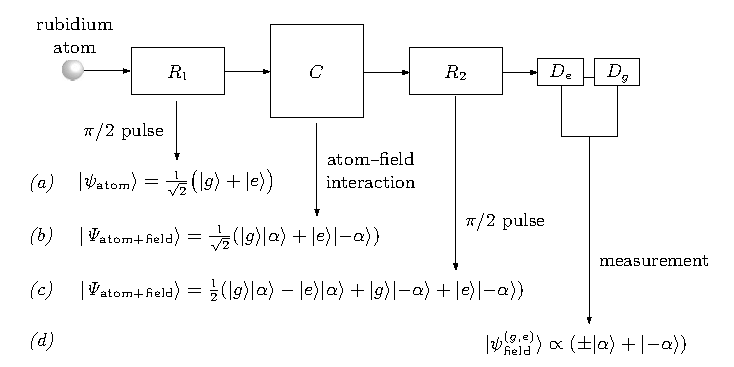
\includegraphics[width=.96\linewidth]{figures/ch06_fig01.pdf}
\caption{猫状態を生成する事象の系列。(a)共振器$R_1$で$\pi/2$パルスを加え、Rb原子を$|g\rangle$と$|e\rangle$の重ね合わせ(6.10)に準備する。(b)コヒーレント場$|\alpha\rangle$を含む共振器Cを通過するとき、原子が$|e\rangle$状態なら、場へ分散的位相シフト$|\alpha\rangle\to|-\alpha\rangle$を与える。原子は$|g\rangle$と$|e\rangle$の重ね合わせなので、もつれた原子・場状態［(6.15)参照］が作られる。(c)共振器$R_2$で、別の$\pi/2$パルスを原子へ加え、原子・場状態(6.17)へ導く。(d)検出器対$D_e$、$D_g$で原子のエネルギー状態$|g\rangle$または$|e\rangle$を測定し、共振器Cの状態を、もつれていない猫状態$|\Psi_{\mathrm{field}}^{(g,e)}\rangle\propto(\pm|\alpha\rangle+|-\alpha\rangle)$へ射影する。}
\end{figure}
\begin{figure}[htbp]\centering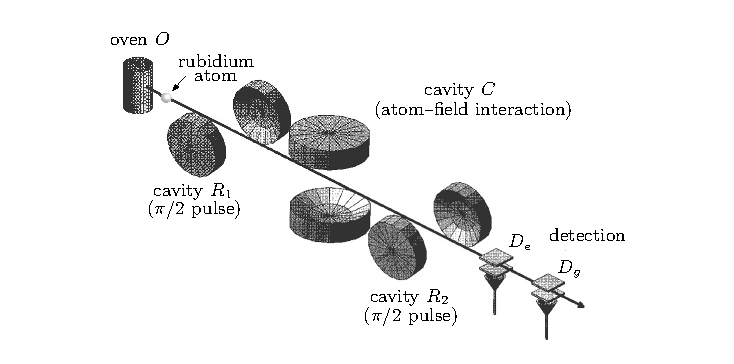
\includegraphics[width=.9\linewidth]{figures/ch06_fig02.pdf}
\caption{放射場の中間的尺度のSchrödingerの猫状態を作り、その漸進的デコヒーレンスを監視するために、Bruneら\cite{ref247}が用いた実験配置。炉Oから放出されたRb原子は、光子場を含む共振器$R_1$、C、$R_2$を順に通過し、電離箱$D_e$、$D_g$で検出される。許可を得て\cite{ref250}の図を改作。Copyright 1996 by the American Physical Society.}
\end{figure}

% 原文 p.249
\hypertarget{srcpage:249}{}\label{srcpage:249}
\begin{equation}
|\psi_{\mathrm{atom}}\rangle=\frac1{\sqrt2}(|g\rangle+|e\rangle)\tag{6.10}
\end{equation}
を作る。初期原子状態が$|g\rangle$なら、最終状態は$|\psi_{\mathrm{atom}}\rangle=(|g\rangle-|e\rangle)/\sqrt2$であっただろう。次に原子は共振器Cへ入る。共振器中の熱放射を最小にするため、Cは絶対零度近くの超伝導領域まで冷却される。共振器$R_1$とは対照的に、Cはいわゆる「Q値」が非常に大きい。Qは``quality''を表す。これは散逸損失が最小限となり、共振器内の光子寿命がかなり長いことを意味する。共振器は、約3cm離れた二枚の平行な鏡からなる。ただし鏡の間隔は調節でき、その結果、共振器内の放射の周波数を変えられる。この放射は、数個の光子を含むコヒーレント場からなる。

共振器の周波数が、準位$|g\rangle$からのいかなる遷移の共鳴周波数からも大きく外れているため、場と相互作用する$|g\rangle$状態には何も起こらない一方、別の準位$|i\rangle$、すなわち$n=52$の円形Rydberg状態を含む、$|e\rangle$からの遷移の周波数には、かなり近いことに注意することが非常に重要である。しかし、原子軌道に沿う場の強度の増減は非常にゆっくりなので、原子と場の相互作用はほぼ断熱的である。つまり、原子と場の間でエネルギー量子は交換されず、状態(6.4)の成分$|e\rangle$の振幅$|c_e(t)|$にも実際の変化は起きない。代わりに起こることが、非常に興味深い。共振器Cへ入った原子は、場に対する屈折媒質として働き、場の周波数にシフト$\delta\omega$を生じさせる。このシフトが有意になるのは原子が$|e\rangle$状態の場合だけで、$|g\rangle$状態では無視できることが分かる。原子と場の相互作用時間$\tau$を微調整することで、実験では、原子が$|e\rangle$状態の場合に、場に$\pi$に近い値の位相シフト$\varphi=\tau\delta\omega$を与える。

各光子へそのような位相シフト$\varphi$を加えると、コヒーレント状態$|\alpha\rangle$はどうなるだろうか。複素振幅$\alpha$の光子場のコヒーレント状態は、光子数固有状態$|n\rangle$の重ね合わせで定義される\cite{ref238,ref239,ref240,ref241}。
\begin{equation}|\alpha\rangle=\sum_{n=0}^\infty c_n|n\rangle,\tag{6.11}\end{equation}
ここで、
\begin{equation}c_n=e^{-|\alpha|^2/2}\frac{\alpha^n}{\sqrt{n!}}.\tag{6.12}\end{equation}
したがって光子数状態の分布は、平均光子数$\bar n=|\alpha|^2$のPoisson分布に従う。
\begin{equation}\wp(n)\equiv|c_n|^2=e^{-\bar n}\left(\frac{\bar n^n}{n!}\right).\tag{6.13}\end{equation}
各光子が位相シフト$\varphi$を受けると、状態$|\alpha\rangle$は、
% 原文 p.250
\hypertarget{srcpage:250}{}\label{srcpage:250}
\begin{equation}
|\alpha\rangle\longrightarrow e^{-|\alpha|^2/2}\sum_{n=0}^\infty e^{in\varphi}\frac{\alpha^n}{\sqrt{n!}}|n\rangle
=e^{-|\alpha|^2/2}\sum_{n=0}^\infty\frac{(e^{i\varphi}\alpha)^n}{\sqrt{n!}}|n\rangle=|e^{i\varphi}\alpha\rangle.\tag{6.14}
\end{equation}
となる。したがって、実験のように$\varphi=\pi$の位相シフトでは、コヒーレント場状態$|\alpha\rangle$は$|-\alpha\rangle$へ変換される。原子が共振器Cを通過した後、複合的な原子・場系は、状態［(6.3)参照］
\begin{equation}|\Psi_{\mathrm{atom+field}}\rangle=\frac1{\sqrt2}(|g\rangle|\alpha\rangle+|e\rangle|-\alpha\rangle)\tag{6.15}\end{equation}
で記述されることになる。図6.2の実験配置へ立ち戻ろう。実際には、$R_1$と同一の第三の共振器$R_2$が、原子軌道に沿って共振器Cの後にある。$R_2$内では、Cから出てきた原子へ、二回目の$\pi/2$パルスを加える。このパルスが、次の変換を実現することを思い出そう［(6.10)参照］。
\begin{equation}\begin{aligned}|g\rangle&\longrightarrow\frac1{\sqrt2}(|g\rangle-|e\rangle),\\|e\rangle&\longrightarrow\frac1{\sqrt2}(|g\rangle+|e\rangle).\end{aligned}\tag{6.16}\end{equation}
したがって、もつれた状態(6.15)は、
\begin{equation}\begin{aligned}
|\Psi_{\mathrm{atom+field}}\rangle&=\frac12(|g\rangle|\alpha\rangle-|e\rangle|\alpha\rangle+|g\rangle|-\alpha\rangle+|e\rangle|-\alpha\rangle)\\
&=\frac12(|\alpha\rangle+|-\alpha\rangle)|g\rangle+\frac12(-|\alpha\rangle+|-\alpha\rangle)|e\rangle.
\end{aligned}\tag{6.17}\end{equation}
となる。$R_2$の通過後、原子は二つの電離箱$D_e$、$D_g$へ入り、$|g\rangle$状態か$|e\rangle$状態かが測定される。状態(6.17)と量子力学の通常の射影公準によれば、測定後の場の状態は、原子が$|g\rangle$状態に見いだされるなら、
\begin{equation}|\psi_{\mathrm{field}}^{(g)}\rangle=\frac1{\mathcal N}(|\alpha\rangle+|-\alpha\rangle),\tag{6.18}\end{equation}
原子が$|e\rangle$状態に見いだされるなら、
\begin{equation}|\psi_{\mathrm{field}}^{(e)}\rangle=\frac1{\mathcal N}(-|\alpha\rangle+|-\alpha\rangle)\tag{6.19}\end{equation}
の、どちらかになる。ここで$\mathcal N$は規格化因子であり、$|\alpha|^2$が大きければ$\sqrt2$に非常に近い。簡単のため、以下では$\mathcal N=\sqrt2$と仮定しよう。

(6.18)、(6.19)から、今や異なる位相を持つ二つのコヒーレント場状態の重ね合わせを、実際に準備できたことが分かる。これらの状態の「猫らしさ」は、共振器C内の平均光子数$\bar n=|\alpha|^2$が増すほど大きくなる。
% 原文 p.251
\hypertarget{srcpage:251}{}\label{srcpage:251}
これらの重ね合わせ状態は、もつれた状態$|\Psi_{\mathrm{atom+field}}\rangle$［(6.15)参照］とは異なることに注意しよう。後者からは、場自体が重ね合わせにあるとはいえず、原子・場の結合系だけが重ね合わせで記述される。これに対して、共振器$R_2$を通過した後の原子状態の測定は、原子と場のもつれを解くので、(6.18)、(6.19)は放射場の真の重ね合わせ状態を表す。

重要な問いが一つ残る。重ね合わせ(6.18)、(6.19)を、対応する混合から、どう区別できるだろうか。これは、上述の方法で中間的尺度のSchrödingerの猫を作ることに成功したと主張するためだけでなく、私たちの主要目標、すなわちデコヒーレンスの作用を観測するためにも重要である。実験では、次節で説明する巧妙な仕掛けによって、この問題を解決する。
\subsubsectionlink{デコヒーレンスの漸進的作用を観測する}
最初の原子の通過と測定は、その状態に関する情報を共振器Cへ残すことに注意しよう。測定結果に応じて、C内の場の最終状態が、$|\psi_{\mathrm{field}}^{(g)}\rangle$または$|\psi_{\mathrm{field}}^{(e)}\rangle$となるからである。(6.18)、(6.19)から分かるように、この情報は、重ね合わせの成分$|\alpha\rangle$と$|-\alpha\rangle$の相対符号に符号化されている。デコヒーレンスは、このような位相情報を環境へ非局在化し、系の水準では利用できなくする傾向があることを知っている。その結果としてのコヒーレンスの減衰を、どう監視できるだろうか。

その仕掛けは、探針として働く第二の原子を、共振器列$R_1\to\mathrm C\to R_2$へ送ることである。第一の原子の通過後、十分速くこれを行えば、第一の原子についての情報は、共振器Cの場の状態へまだよく符号化されており、第二の原子はこの情報と相関する。注目すべき結果は、デコヒーレンスがなく、光子数が$\bar n=|\alpha|^2\gg1$なら、$D_e$または$D_g$での検出後、第二の原子は常に第一の原子と同じ状態に見いだされることである。

実際にそうなることは、次の簡単な計算から容易に分かる（図6.3参照）。原子1が$|e\rangle$状態で検出され、場の状態が$|\psi_{\mathrm{field}}^{(e)}\rangle$となったと仮定しよう。共振器$R_1$を通過した原子2は、重ね合わせ$|\psi_{\mathrm{atom2}}\rangle=(|g\rangle+|e\rangle)/\sqrt2$［(6.10)参照］で記述される。ここでは、基底状態$|g\rangle$と$|e\rangle$は原子2を指す。したがって、この原子と場の、初めの無相関な状態は、
\begin{equation}|\Psi_{\mathrm{atom2+field}}\rangle=\frac12(|g\rangle+|e\rangle)(-|\alpha\rangle+|-\alpha\rangle).\tag{6.20}\end{equation}
原子2が共振器Cを通ると何が起きるだろうか。原子が$|e\rangle$状態なら、場の状態は位相シフト$|\pm\alpha\rangle\to|\mp\alpha\rangle$を受けることを思い出そう。したがって、Cを通過した後の結合状態は、
% 原文 p.252
\hypertarget{srcpage:252}{}\label{srcpage:252}
\begin{equation}|\Psi_{\mathrm{atom2+field}}\rangle=\frac12(-|g\rangle|\alpha\rangle+|g\rangle|-\alpha\rangle-|e\rangle|-\alpha\rangle+|e\rangle|\alpha\rangle).\tag{6.21}\end{equation}
となる。次に原子は共振器$R_2$を通過し、$|g\rangle$と$|e\rangle$がこれらの状態の重ね合わせへ変換される［(6.16)参照］。したがって状態(6.21)は、
\begin{equation}\begin{aligned}
|\Psi_{\mathrm{atom2+field}}\rangle
&=\frac1{2\sqrt2}\bigl(-|g\rangle|\alpha\rangle+|e\rangle|\alpha\rangle+|g\rangle|-\alpha\rangle-|e\rangle|-\alpha\rangle\\
&\qquad-|e\rangle|-\alpha\rangle-|g\rangle|-\alpha\rangle+|e\rangle|\alpha\rangle+|g\rangle|\alpha\rangle\bigr)\\
&=\frac1{\sqrt2}|e\rangle(|\alpha\rangle-|-\alpha\rangle).
\end{aligned}\tag{6.22}\end{equation}
となる。$|\alpha\rangle$と$|-\alpha\rangle$が直交すると仮定すれば、共振器C内の光子数$\bar n=|\alpha|^2$が増すほどよい近似となるが、状態(6.22)に対応する原子2の縮約密度演算子は、
\begin{equation}
\hat\rho_{\mathrm{atom2}}=\operatorname{Tr}_{\mathrm{field}}|\Psi_{\mathrm{atom2+field}}\rangle\langle\Psi_{\mathrm{atom2+field}}|=|e_2\rangle\langle e_2|.\tag{6.23}
\end{equation}
直ちに、原子1が$|e\rangle$状態で検出されたとき、原子2を$|e\rangle$状態に見いだす確率$P_{ee}$は、$P_{ee}=1$となる。
% 原文 p.253
\hypertarget{srcpage:253}{}\label{srcpage:253}
原子1が$|g\rangle$状態で検出されたという仮定の下でも、同様の計算ができる。これで、二原子の完全な相関についての、上の主張が確立された。

\begin{figure}[htbp]\centering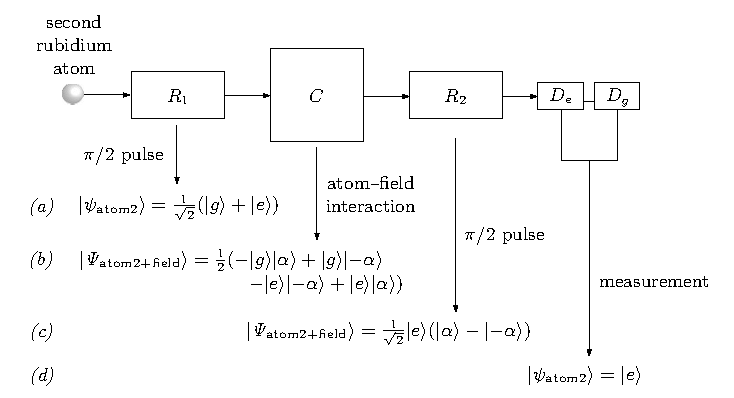
\includegraphics[width=.96\linewidth]{figures/ch06_fig03.pdf}
\caption{第一の原子が$|e\rangle$状態で検出されたと仮定したとき、共振器C内の場の重ね合わせ状態を検出し、そのデコヒーレンスを監視する事象の系列。(a)共振器$R_1$の$\pi/2$パルスが、第二のRb原子を$|g\rangle$、$|e\rangle$の重ね合わせ(6.20)に準備する。(b)原子は、第一の原子の通過後、重ね合わせ状態に残された共振器Cへ入る。原子2はC内の場へ別の位相シフトを与え、もつれた原子・場状態［(6.21)参照］を作る。(c)共振器$R_2$の$\pi/2$パルスが、場と原子のもつれを解く［(6.22)参照］。(d)場の状態$|\pm\alpha\rangle$が近似的に直交するなら、原子2は常に、原子1と同じ$|e\rangle$状態で検出される。したがって、二つの測定結果は完全に相関する。この相関の減衰は、共振器Cの猫状態のデコヒーレンスを意味する。}
\end{figure}

ゆえに、猫状態のデコヒーレンスを観測するために必要なのは、第一、第二の原子を送り出す時間間隔$T$を増やしながら、原子対の測定結果間の相関$P_{ee}(T)$、あるいは$P_{gg}(T)$の減衰を測定することだけである。$T$が場の重ね合わせの特徴的なデコヒーレンス時間よりはるかに小さければ、$P_{ee}(T)$は1に近くなる。重ね合わせがまだほとんどデコヒーレンスしていないときの、測定結果間の完全な相関を反映するのである。遅延時間$T$を長くすると、共振器内の重ね合わせは、ますますデコヒーレンスする。やがて、すべての相対位相情報、したがって第一の原子の状態の情報が環境へ非局在化し、場は非コヒーレントな統計的混合
\begin{equation}\hat\rho_{\mathrm{field}}=\frac12(|\alpha\rangle\langle\alpha|+|-\alpha\rangle\langle-\alpha|)\tag{6.24}\end{equation}
で記述される。このとき、第一、第二の原子の測定結果は完全に無相関となる。すなわち、第二の原子の測定結果はランダムであり、第一の原子の測定結果から独立になる。したがって、このデコヒーレンス過程は、$P_{ee}(T)$が$1/2$まで減衰することとして観測できる。

図6.4は、$P_{ee}(T)$の理論予測\cite{ref250}を示し、これは実験観測\cite{ref251}と非常によく一致した。$P_{ee}(T)$が初期値1からかなり急速に低下し、完全なデコヒーレンスに対応する$P_{ee}(T)=1/2$の平坦部に達する様子が明瞭に見える。読者は、$P_{ee}(T)$がある範囲の遅延時間$T$にわたり$1/2$付近にとどまった後、より大きい$T$で、なぜ突然また0へ向かって減衰するのかと、疑問に思うかもしれない。説明は非常に簡単である。共振器C内の光子寿命は有限なので、やがてC内に光子がなくなる。すると、Cを通過する原子に対する効果はなくなる。この場合、原子が受けるのは、共振器$R_1$と$R_2$の二つの$\pi/2$パルスだけであり、それらの合成効果は、初期状態$|e\rangle$を$|g\rangle$へ変換することである［(6.16)参照］。
\begin{equation}|e\rangle\xrightarrow{\pi/2}\frac1{\sqrt2}(|g\rangle+|e\rangle)\tag{6.25}\end{equation}
\begin{equation}\xrightarrow{\pi/2}\frac1{\sqrt2}\left[\frac1{\sqrt2}(|g\rangle-|e\rangle)+\frac1{\sqrt2}(|g\rangle+|e\rangle)\right]=|g\rangle.\tag{6.26}\end{equation}
したがって、原子は決して$|e\rangle$状態で検出されず、$T\to\infty$で$P_{ee}(T)\to0$となる。

図6.4のグラフから、場の重ね合わせの特徴的デコヒーレンス時間を読み取れる。実験では、それが二つの主要パラメーターに依存することが示された。
% 原文 p.254
\hypertarget{srcpage:254}{}\label{srcpage:254}
\begin{figure}[htbp]\centering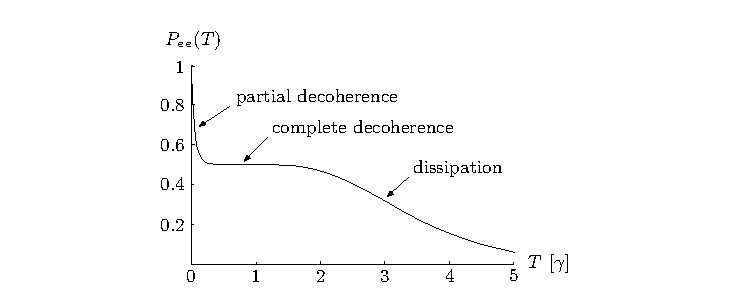
\includegraphics[width=.85\linewidth]{figures/ch06_fig04.pdf}
\caption{Davidovichら\cite{ref250}による、一対の原子が通過する遅延時間$T$への、同時確率$P_{ee}(T)$の依存性。初期の速い減衰は、共振器Cの猫状態のデコヒーレンスに対応し、$P_{ee}(T)=1/2$は完全なデコヒーレンスを表す。さらに大きな$T$では、共振器からの光子漏出によって$P_{ee}(T)$がさらに低下する。遅延時間$T$の単位は、共振器の特徴的散逸期間$\gamma$である。許可を得て\cite{ref250}の図を改作。Copyright 1996 by the American Physical Society.}
\end{figure}
\begin{enumerate}
\item 共振器Cを通過する$|e\rangle$状態の原子が、場へ誘起する位相シフト$\varphi$。$\varphi$が大きいほど、場の重ね合わせのデコヒーレンス時間が短いことが分かった。これはもっともである。重ね合わせ状態の「猫らしさ」は、各成分をどれほど識別できるかに依存する。$\varphi$が小さければ、場の状態$|\alpha\rangle$と$|e^{i\varphi}\alpha\rangle$［(6.14)参照］の重なりは大きい。他方、$\varphi$が最大値$\pi$へ近づくと、これは上の議論で仮定した値であり、実験で達成した位相シフトにも近いが、二状態は直交し、したがって最大限に区別される。
\item 共振器C内の平均光子数$\bar n=|\alpha|^2$。これも理にかなっている。光子が多いほど、状態$|\Psi_{\mathrm{field}}^{(g,e)}\rangle$［(6.18)参照］は、より中間的尺度のもの、最終的には巨視的なものとなり、したがって、より強くデコヒーレンスを受ける。また、与えられた位相シフト$\varphi$について、$\bar n$が大きいほど成分$|\alpha\rangle$と$|e^{i\varphi}\alpha\rangle$の重なりは小さくなり、より区別される。
\end{enumerate}
Bruneたちは実験でこれらのパラメーターを変え、デコヒーレンス率がそれに応じて変わる様子を観測した。注目すべきことに、結果はDavidovichら\cite{ref250}の理論予測と驚くほどよく一致した。中間的尺度の「Schrödingerの子猫」を生成し、存在を検証し、そのデコヒーレンスを制御された仕方で観測したのは、これが初めてであった。

% 原文 p.255
\hypertarget{srcpage:255}{}\label{srcpage:255}
Bruneたちが行った型の実験は、その後、さらに多くの実験を生み、上述の結果が確認され、拡張されてきた。たとえば、共振器CのQ値を改善する必要があるが、その光子数を増すことで、ますます大きな猫状態を作れる。最近の実験では、数十個の光子が使われている\cite{ref252}。この種の実験は一般に「共振器量子電気力学」、略して「共振器QED」と呼ばれる。Schrödingerの猫状態の生成と、そのデコヒーレンスの観測だけでなく、共振器QEDは、量子コンピューターの実現にも使える可能性がある。さらに学びたい読者には、Dutraの本\cite{ref253}が、よい、しかも楽しく読める入門となる。

\subsubsectionlink{Schrödingerの猫を生き返らせる}
デコヒーレンスが完全にユニタリーで、したがって原理的に可逆な過程であるにもかかわらず、私たちは量子から古典への移行を「一方通行」と考えがちである。量子コヒーレンスが失われると、物体は古典的に振る舞い、量子世界へ戻すものは何もないように見える。もちろん、2.7節のデコヒーレンスの一般的議論から、それがあらゆる実用的目的について不可逆とみなされる理由を知っている。系の水準へ重ね合わせを実際に「再局在化」する、すなわちデコヒーレンス過程を実効的に時間反転するには、環境を適切に制御しなければならず、それは通常、実際には不可能だからである。

2.13節では、完全に制御できるよう適切に設計した「人工的」環境と系を相互作用させることで、仮想的デコヒーレンスの一例である、真に可逆なデコヒーレンス過程を調べられることを指摘した。1997年、Bruneのグループ\cite{ref254}は、前の各節の共振器QED実験を修正し、そのような設計された環境を含める案を提案した。2007年現在、この提案はまだ実験的に実現されていない。主な理由は、二つの超伝導共振器の間の可逆的結合が必要で、それを実際に実現するのが難しいからである。それでも、実験の考え方は非常に興味深く、技術的障害が近い将来に克服される見込みも高いため、本節で提案を概説する。

実験配置は、基本的に前述のものと同じである（図6.2参照）。主要な違いは、超伝導共振器Cを、たとえば超伝導導波路を用いて、初め空の、第二の同一共振器$\mathrm C_2$へ線形結合することである。追加の$\mathrm C_2$と明瞭に区別するため、以下では最初の共振器Cを$\mathrm C_1$と呼ぶ。この結合によって、$\mathrm C_1$と$\mathrm C_2$はエネルギー、すなわち光子を交換できる。Rb原子が装置を通過し、その状態が$D_e$、$D_g$で測定された後、共振器$\mathrm C_1$は二つの場の状態$|\alpha\rangle$、$|-\alpha\rangle$の重ね合わせに残されること［(6.18)、(6.19)参照］、
% 原文 p.256
\hypertarget{srcpage:256}{}\label{srcpage:256}
そして、二成分の相対符号が、測定された原子状態の情報を符号化することを思い出そう。

二共振器の結合によって、この位相情報が「貯蔵庫」$\mathrm C_2$へ移ったとする。このとき$\mathrm C_1$の状態は、対応して混合(6.24)で記述されなければならない。提案の考え方は、$\mathrm C_1$と$\mathrm C_2$の結合が十分高い程度まで可逆なら、その後この情報伝達の向きを逆転し、$\mathrm C_1$の初期重ね合わせを回復するとともに、$\mathrm C_2$を初期の空の状態へ戻せる、というものである。こうして、$\mathrm C_2$が$\mathrm C_1$に対する制御可能な単一モード環境として働き、$\mathrm C_1$のSchrödingerの猫状態をデコヒーレンスさせ、その後再出現させる、可逆なデコヒーレンス過程を模擬できる。

この議論をもう少し精密にしよう。二共振器間で、エネルギーが周波数$\Omega_{\mathrm C}$で振動的に交換されるとする。この周波数は、$\mathrm C_1$の猫状態の準備時間が、エネルギー交換の一周期よりはるかに短くなるよう選ぶ。したがって、二共振器の結合は重ね合わせ状態の準備に影響しないと仮定する。結合は線形なので、$\mathrm C_1$のコヒーレント場$|\alpha(t)\rangle$は、$\mathrm C_2$に別のコヒーレント場$|\beta(t)\rangle$を生じさせる。$t=0$で$\mathrm C_2$が場を含まないことを考慮すると、$\alpha(t)=\alpha_0\cos(\Omega_{\mathrm C}t/2)$、$\beta(t)=\alpha_0\sin(\Omega_{\mathrm C}t/2)$と書ける。したがって、$\mathrm C_1$の初期猫状態［(6.18)、(6.19)参照］
\begin{equation}|\Psi_{\mathrm C_1}^{(g,e)}\rangle=\frac1{\mathcal N}(\pm|\alpha\rangle+|-\alpha\rangle)\tag{6.27}\end{equation}
は、結合系$\mathrm C_1+\mathrm C_2$のもつれた状態へ発展する。
\begin{equation}|\Psi_{\mathrm C_1+\mathrm C_2}^{(g,e)}\rangle=\frac1{\mathcal N}(\pm|\alpha(t)\rangle|\beta(t)\rangle+|-\alpha(t)\rangle|-\beta(t)\rangle).\tag{6.28}\end{equation}
その後の振る舞いは、二つのコヒーレント場状態$|\pm\alpha\rangle$の重なりが、平均光子数$\bar n=|\alpha|^2$が増すほど減少することから、容易に理解できる。時間$t=\pi/\Omega_{\mathrm C}$後には$\beta(t)=\alpha_0$となり、すべての光子が$\mathrm C_2$に集中する。したがって$|\pm\beta\rangle$は最大限に区別され、$|\pm\alpha\rangle$の識別可能性は最小になる。これは、重ね合わせ成分の相対符号についての情報を、$\mathrm C_1$の犠牲の下で、$\mathrm C_2$が最大限保持することを意味する。言い換えれば、$\mathrm C_1$だけへのどのような測定からも、相対符号について何も分からない。$\mathrm C_2$が位相情報を運び去り、$\mathrm C_1$は形式的に、$|\pm\alpha\rangle$の非コヒーレント混合(6.24)で記述される。

読者は、この状況が、環境に対応する状態が急速に直交し、系の密度行列で相対位相情報が減衰する、通常のデコヒーレンス過程の記述（2.7節参照）と、まさに類似していると気づくだろう。
% 原文 p.257
\hypertarget{srcpage:257}{}\label{srcpage:257}
ここでは$\mathrm C_2$が、まさに環境の役割を果たすため、この類似は予想どおりである。しかし、ここでの提案の決定的な違いは、特徴的時間$\tau=2\pi/\Omega_{\mathrm C}$、すなわち二共振器間のエネルギー交換周期後に、過程が完全に逆転することである。今や$|\pm\alpha\rangle$は、$t=0$と同じく再び最大限に区別される。相対符号についてのすべての情報を$\mathrm C_1$から取り出せ、$\mathrm C_2$の場の重ね合わせのコヒーレンスは回復している。

この漸進的デコヒーレンスと再コヒーレンスは、以前とまったく同じ方法、すなわち第二の原子を装置へ送り、二原子の通過の遅延時間$T$に対する同時確率$P_{ee}(T)$の依存性を測定することで観測できる。$\mathrm C_1$と$\mathrm C_2$の結合以外のデコヒーレンス源を無視すれば、$P_{ee}(T)$は、$n=1,2,\ldots$に対する時刻$T_n=n\tau=2n\pi/\Omega_{\mathrm C}$に、周期的に初期値1へ戻ると予想される。これらの時刻には、$\mathrm C_1$の猫状態のデコヒーレンスは完全に取り消されている。逆に、間隔$n\tau/2=n\pi/\Omega_{\mathrm C}$では、$\mathrm C_1$は非コヒーレント混合で記述され、原子1、2の測定結果は完全に無相関となり、$P_{ee}(n\tau/2)=1/2$となる。

この振る舞いを図6.5に示す。同時確率$P_{ee}(T)$を直接描く代わりに、Raimond、Brune、Haroche\cite{ref254}が最初に導入した、二原子相関関数$\eta(T)$を用いた。この関数は完全相関では$1/2$、完全なデコヒーレンスでは0となる。遅延時間が、特徴的時間$\tau=2\pi/\Omega_{\mathrm C}$の整数倍に等しいと、初期状態が回復し、コヒーレンスの復活が得られることが分かる。
\begin{figure}[htbp]\centering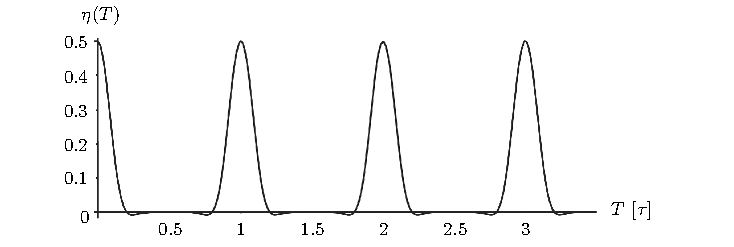
\includegraphics[width=.94\linewidth]{figures/ch06_fig05.pdf}
\caption{Raimond、Brune、Haroche\cite{ref254}が提案した再コヒーレンス実験における、遅延時間$T$に対する二原子相関関数$\eta(T)$の依存性。第二の共振器$\mathrm C_2$、すなわち貯蔵庫によって、$\mathrm C_1$からコヒーレンスが連続的に取り出され、戻される。これが$\mathrm C_1$の猫状態の周期的復活と、最大相関信号$\eta(T)=1/2$の再出現を生む。$T$の単位は、二共振器間でエネルギー、したがって位相情報を交換する特徴的周期$\tau=2\pi/\Omega_{\mathrm C}$である。$\mathrm C_1$の初期場は、平均5個の光子を含むとした。}
\end{figure}

% 原文 p.258
\hypertarget{srcpage:258}{}\label{srcpage:258}
もちろん、現実的な実験設定では、この復活過程は永遠には続かない。共振器$\mathrm C_1$と$\mathrm C_2$は、鏡面での光子損失のような、ほかのデコヒーレンス源や散逸効果を受けるからである。これらの過程は、図6.5の復活ピークの振幅を指数関数的に減衰させることが示されており\cite{ref255}、実際に数個以上のピークを観測できる見込みは低い。それでも、一つの復活ピークの観測だけでも、デコヒーレンスが少なくとも原理的には完全に可逆である事実を、印象的に実験で示すことになる。

\subsectionlink{$\mathrm C_{70}$分子による干渉実験}
本節では、University of ViennaのAnton Zeilingerのグループが行った、一連の実験を述べる。これらは本質的に、よく知られた二重スリット実験を高度に改良したものである。しかしここでは、光や電子のような微視的実体の代わりに、重い分子の干渉模様を観測する。これらの実験が注目すべきなのは、二つの理由による。第一に、通常なら明らかに「物質」の分類に入る物体の、量子的な「波動性」を示す。第二に、デコヒーレンスの連続的作用が、これらの物体から「量子性」を徐々に奪い、経験するおなじみの古典的物体へ変える様子を直接示す。詳しく述べる前に、先行する実験、すなわち単一電子で行われた二重スリット実験を、まず数段落で概説しよう。

\subsubsectionlink{電子による二重スリット実験}
2002年、Physics Worldの読者に、史上「最も美しい物理実験」を選ぶよう求めたところ、一位になったのは、単一電子による二重スリット実験\cite{ref256}だった。Feynmanは、二重スリット実験は「その中に量子力学の核心があり、実際、それは理論の唯一の謎を含む」現象であると述べたことで有名である\cite{ref257}。確かに、量子力学の奇妙な特徴を、これほど単純かつ完全に体現する、ほかの実験を想像するのは難しい。

興味深いことに、電子が二重スリットを通るという元の形でこの実験が実際に行われたのは、1961年、University of TübingenのGottfried Möllenstedtの学生、Claus Jönsson\cite{ref258,ref259}によってであった。Möllenstedtは、それ以前に、電子ビプリズムという別の装置、本質的には電子ビームを二分する非常に細い線を使い、電子の干渉を実験的に示していた。この方法は、19世紀初頭に英国の科学者Thomas Youngが、日光のビームを分け、光が波動的な強め合い・弱め合いの干渉効果を示すことを実証した実験\cite{ref260}で使った、紙片に似ている。
% 原文 p.259
\hypertarget{srcpage:259}{}\label{srcpage:259}
さらに意外かもしれないが、装置内に常に単一電子しかないことを保証した実験は、1989年になって初めて、HitachiのAkira Tonomuraたちが、Möllenstedtと同じく電子ビプリズムを用いて行った\cite{ref261}。得られた干渉模様を図6.6に示す。この実験は、干渉縞が電子間の相互作用で生じるのではなく、個々の電子の波動性によることを示し、量子力学の「謎」を明瞭に反映する。電子ビプリズム干渉計のデコヒーレンスは、最近SonnentagとHasselbach\cite{ref262}が調べた。彼らは、電子と、巨視的で散逸的な電子気体・フォノン気体環境とのCoulomb相互作用によって、干渉模様の可視度が減衰する様子を研究した。

\subsubsectionlink{実験配置}
重い分子の波動性を示すために、Zeilingerのグループが用いた実験配置を概説しよう。Markus Arndtたち\cite{ref263}が1999年のNature論文で報告した最初の実験では、その形から「バッキーボール」と呼ばれることの多い、$\mathrm C_{60}$分子が使われた（図6.7参照）。その後、Zeilingerのグループが2002年の論文\cite{ref264}で初めて結果を報告した実験は、さらに大きな、細長いバッキーボール形の$\mathrm C_{70}$分子と、異なる実験配置\cite{ref264,ref265,ref266,ref267}を用いて行われた。以下では、この後の一連の実験に基づいて論じる。

まず、$\mathrm C_{70}$分子が、電子などの微視的実体に比べて、どれほど重いかを実感しよう。
\begin{figure}[htbp]\centering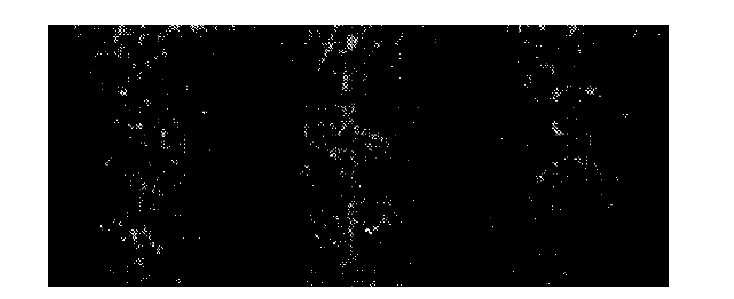
\includegraphics[width=.85\linewidth]{figures/ch06_fig06.pdf}
\caption{Tonomuraたち\cite{ref261}の二重スリット実験で得られた、単一電子の干渉模様。許可を得て\cite{ref261}から転載。Copyright 1989 American Institute of Physics.}
\end{figure}
% 原文 p.260
\hypertarget{srcpage:260}{}\label{srcpage:260}
各炭素原子は6個の陽子、6個の中性子、6個の電子を含むので、$\mathrm C_{70}$分子は合計1000個以上の微視的構成要素からなる。各分子は、高度に励起された内部回転・振動自由度を非常に多数持つ。このため、個々の分子に有限の温度を割り当てることができる。また、分子からの熱放射、すなわち光子の放出も観測できる\cite{ref267}。したがって、$\mathrm C_{70}$分子は、明らかに「粒子」の分類に入るように見える。
\begin{figure}[htbp]\centering
\includegraphics[width=.65\linewidth]{figures/ch06_fig07.pdf}
\caption{Arndtら\cite{ref263}の最初の物質波干渉実験で用いられた、$\mathrm C_{60}$分子の模式図。60個の炭素原子が、直径約1nmのバッキーボール形に並んでいる。}
\end{figure}

このような重い分子の干渉効果を観測するのは、なぜ難しいのだろうか。関係する量は、物質のde Broglie波長$\lambda=h/(mv)$であり、$m$、$v$はそれぞれ粒子の質量と速度である。したがって、粒子が重く速いほど、波長は短い。二重スリット型の実験で粒子の干渉を観測するには、スリット間隔、まして各スリットの幅が、波長程度でなければならない。実験の$\mathrm C_{70}$分子の典型的速度、約$100\,\mathrm{m/s}$では、de Broglie波長はわずか数pmである。このような狭いスリットを、これほど狭い間隔で作ることが不可能なのは、容易に想像できるだろう。

この困難をどう克服できるだろうか。Zeilingerのグループは、いわゆるTalbot--Lau効果に基づく、巧みな仕掛けで解決する。その基本原理は次のとおりである（図6.8参照）。平面波$f(z)=e^{2\pi iz/\lambda}$が、$+z$方向に進むとする。この入射波に直角に、平行なスリットの列からなる格子を置く。隣り合うスリットの間隔を$d$とする。このとき、格子の後方の距離
\begin{equation}L_\lambda=\frac{d^2}{\lambda}\tag{6.29}\end{equation}
の整数倍のところで、波の形が実際に格子模様と等しくなることを示せる。ここでは導かないが、短い導出は\cite{ref268}を参照されたい。言い換えれば、格子の後方$nL_\lambda$、$n=1,2,\ldots$の距離にスクリーンを置き、光で実験すると、
% 原文 p.261
\hypertarget{srcpage:261}{}\label{srcpage:261}
間隔$d$の明暗の帯が現れ、格子自体の像を作る。このTalbot--Lau効果は、真の干渉現象である。したがって、物質粒子で同じ実験を行い、「Talbot長」$L_\lambda$の整数倍のところに、格子模様と等しい密度模様を観測すれば、粒子の波動性を示したことになる。ただし、原理的には、格子が単に光線を遮る、いわゆるMoiré効果でも縞が生じる。しかしMoiré模様は波長$\lambda$に依存しない。ゆえに、本当にTalbot--Lau効果かを確かめるには、$\lambda$を変えながら模様の変化を観測すればよい。物質波の場合、$\lambda=h/(mv)$なので、粒子の平均速度$v$を変えることで実現する。
\begin{figure}[htbp]\centering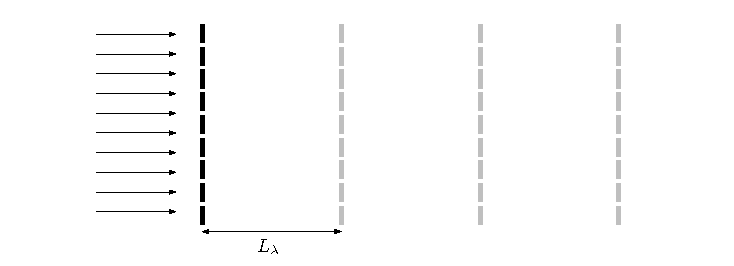
\includegraphics[width=.85\linewidth]{figures/ch06_fig08.pdf}
\caption{Talbot--Lau効果。左の格子を通る平面波は、格子から距離$nL_\lambda$、$n=1,2,\ldots$のところに、格子の像を作る。}
\end{figure}

簡単な評価から、$\mathrm C_{70}$分子の干渉効果を検出するTalbot--Lau法の利点を、直ちに納得できる。Zeilingerのグループの実験では、格子間隔$d$は約$1\,\mu\mathrm m$、分子波長は数pmである。したがって$L_\lambda\sim(10^{-6}\,\mathrm m)^2/(10^{-12}\,\mathrm m)=1\,\mathrm m$となり、干渉模様を観測するには、格子の後方の巨視的距離$L_\lambda$に、「スクリーン」、すなわち粒子検出器を置くだけでよい。実際の実験距離は$L_\lambda=38\,\mathrm{cm}$である。そこで分子速度を変えたとき、特徴的な波長依存性を示す、周期$d$の粒子密度変化を測定すれば、分子の波動性を確認したことになる。

実験配置を図6.9に示す。$\mathrm C_{70}$分子は源から放出され、同一の自立型金格子を三枚通る。各格子は、周期$d=990\,\mathrm{nm}$のスリットを1000本程度含む。最初の格子は、回折模様が観測できるよう、ビームへ一定のコヒーレンスを与える。中央の格子が、実際の回折格子として働く。最後に第三の格子を、回折格子の後方、Talbot長$L_\lambda$の距離に置く。
% 原文 p.262
\hypertarget{srcpage:262}{}\label{srcpage:262}
これは、分子が実際に波動性を持つなら、第三格子の位置で回折格子自体の像となる、干渉模様が得られることを意味する。すなわち、分子密度は$x$方向に周期的な極大と極小を持ち、ピークはスリット間隔$d$だけ離れる。第三格子は、この分子密度模様を走査するマスクである。干渉模様があれば、格子を$x$方向へ動かすと、その後方で記録される分子数が最大値と最小値の間で変動する。したがって、第三格子後方の分子数を、格子の$x$位置の関数として数えることで、この変動を容易に測れる。
\begin{figure}[htbp]\centering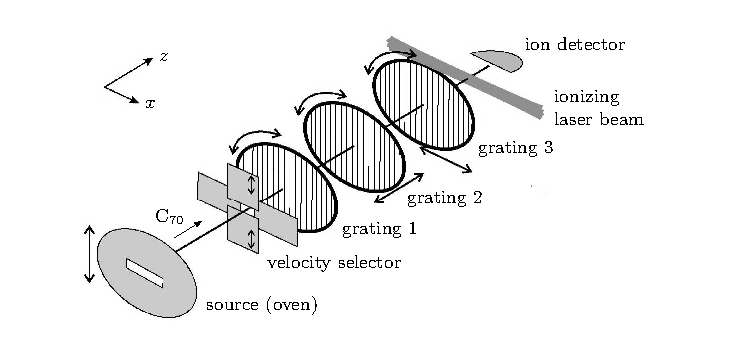
\includegraphics[width=.85\linewidth]{figures/ch06_fig09.pdf}
\caption{Zeilingerのグループの実験\cite{ref264,ref265,ref266,ref267}で、$\mathrm C_{70}$分子の物質波干渉を観測する配置。許可を得て\cite{ref264}の図を改作。Copyright 2002 by the American Physical Society.}
\end{figure}

装置を通る分子の平均速度は、分子源の位置を変え、自由飛行放物線を描くビームの異なる部分を、固定高さの制限器で選ぶことで、約90から$220\,\mathrm{m/s}$の間で調整できる。これらは、de Broglie波長2から6pmに対応する。分子と他粒子の衝突を最小にするため、装置全体は真空槽に収められている。

\subsubsectionlink{重い分子の波動性を確かめる}
典型的な実験一回の結果を図6.10に示す。横軸は走査マスクの$x$軸方向の位置（図6.9参照）、縦軸は各位置における格子後方の分子密度である。$\mathrm C_{70}$分子密度の振動が明瞭に見え、空間的コヒーレンスと干渉効果の存在を確認できる。
% 原文 p.263
\hypertarget{srcpage:263}{}\label{srcpage:263}
分子速度を変え、Talbot--Lau理論に一致する密度模様の変化を観測することで、この模様が実際にTalbot--Lau効果によることも明示的に確認された。
\begin{figure}[htbp]\centering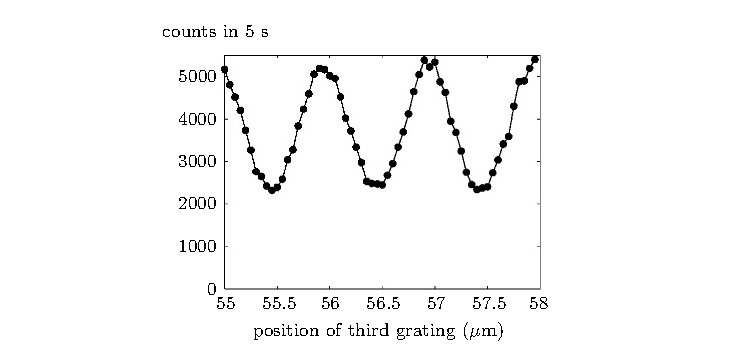
\includegraphics[width=.82\linewidth]{figures/ch06_fig10.pdf}
\caption{Zeilingerのグループの実験で観測された、$\mathrm C_{70}$分子の干渉縞。実線は理論予測に基づいて当てはめた正弦曲線である。許可を得て\cite{ref264}の図を改作。Copyright 2002 by the American Physical Society.}
\end{figure}

また、干渉効果は厳密な一粒子効果であり、異なる分子間の干渉によるものではない。理由は二つある。第一に、粒子間干渉には、相互作用する分子が同じ状態である必要がある。しかし、各$\mathrm C_{70}$分子は非常に多数の内部自由度を持つため、その可能性は実効的にゼロである。第二に、二分子間の距離は、いかなる分子間力の範囲よりもはるかに大きく、したがって、本質的に、どの瞬間にも装置を通っているのは単一分子だけである。

\subsubsectionlink{経路情報とデコヒーレンス}
それでは、本章の主要主題である、デコヒーレンスの実験観測へ移ろう。$\mathrm C_{70}$干渉実験では、デコヒーレンスは主として、分子と背景気体の分子の衝突による。真空は完全ではないので、背景気体は装置内にある程度常に存在する。このような衝突デコヒーレンスは第3章で詳しく述べ、自然界に普遍的にある源であることを示した。しかし、本章冒頭で述べたように、中間的尺度や巨視的物体では、それが通常あまりに速く、その漸進的作用を観測することは実効的に不可能である。
% 原文 p.264
\hypertarget{srcpage:264}{}\label{srcpage:264}
ここに、$\mathrm C_{70}$干渉実験の主要な利点がある。背景気体密度を変えることで、衝突デコヒーレンスの量を精密に調整できる。図6.11は、Lucia Hackermüllerら\cite{ref268}が報告した、背景気体の二つの圧力、すなわち密度で実験的に測定された干渉模様である（\cite{ref265}も参照）。左の図では、干渉縞が明瞭に見える。背景気体の圧力を高めると、縞が目立たなくなる（右）。圧力$p$における干渉模様の可視度$V(p)$を、その最大振幅$c_{\max}(p)$と最小振幅$c_{\min}(p)$の相対差として定量化しよう。
\begin{equation}V(p)=\frac{c_{\max}(p)-c_{\min}(p)}{c_{\max}(p)+c_{\min}(p)}.\tag{6.30}\end{equation}
デコヒーレンスも他の実験的不完全さもない理想的場合には、$c_{\min}=0$で、完全な可視度を得る。完全にデコヒーレンスした場合、干渉模様は観測できず、$c_{\max}=c_{\min}$となるので、可視度はゼロである。

気体圧力$p$に対する可視度(6.30)の変化の実験データ\cite{ref265,ref268}を、図6.12に示す。可視度は$p$とともに指数関数的に低下する。縦軸が対数目盛であることに注意されたい。この指数減衰は、理論計算\cite{ref160,ref269}と見事に一致する。
\begin{figure}[htbp]\centering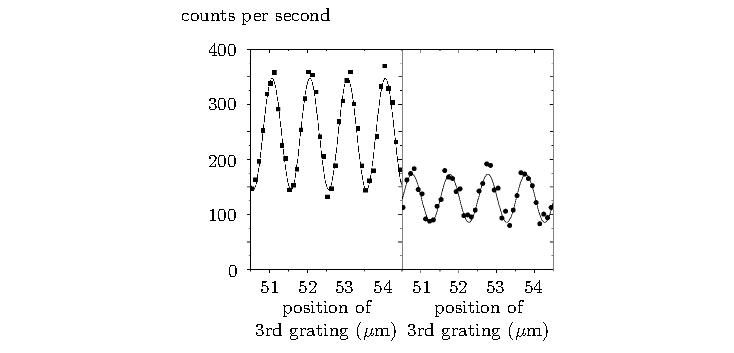
\includegraphics[width=.86\linewidth]{figures/ch06_fig11.pdf}
\caption{Zeilingerのグループの実験\cite{ref268}で観測された、背景気体分子との衝突が誘起するデコヒーレンスによる、$\mathrm C_{70}$分子干渉の減少。左から右へ気体圧力を高めると、干渉縞の可視度が低下する。Springer Science and Business Mediaのご厚意により、許可を得て\cite{ref268}の図を改作。}
\end{figure}
% 原文 p.265
\hypertarget{srcpage:265}{}\label{srcpage:265}
\begin{figure}[htbp]\centering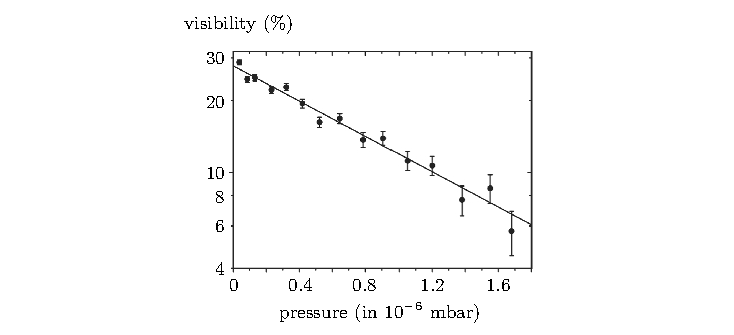
\includegraphics[width=.82\linewidth]{figures/ch06_fig12.pdf}
\caption{Zeilingerのグループ\cite{ref268}が報告した、背景気体圧力への干渉模様の可視度(6.30)の依存性。測定値（円）は、圧力に対する指数減衰を記述する理論予測（実線）によく一致する。Springer Science and Business Mediaのご厚意により、許可を得て\cite{ref268}の図を改作。}
\end{figure}
したがって、これらの実験は、干渉の観測に必要な量子コヒーレンスを、環境との相互作用が徐々に非局在化する様子を、印象的かつ直接に示す。この過程は完全に制御されている。たとえば背景気体の密度を変え、環境が得る経路情報量を変化させれば、デコヒーレンスの量、したがって量子的特徴の喪失を、精密に調整できる。こうして、量子・古典境界を滑らかに行き来して探索でき、観測が理論予測と極めてよく一致することが分かる。

\subsubsectionlink{熱放射の放出によるデコヒーレンス}
巨視的物体の最も重要なデコヒーレンス機構は何だろうか。これまで見たように、光子や空気分子など、他粒子との衝突は確かに普遍的にあり、決定的な役割を果たす。しかし、この長さ尺度でのもう一つの基本的な源は、熱放射の放出である。どの「大きな」物体も、多数の内部自由度へエネルギーを蓄えられる。巨視的物体は、本質的に絶えず光子を吸収し放出する。各放出光子は、物体の経路の情報を運び去り、位置基底でのデコヒーレンス、したがって物体の空間的局在化を生じさせる。

巨視的物体では、熱放射の放出は通常、空間的干渉効果を観測する可能性を完全に閉ざすほど強い。興味深いことに、以下で見るように、$\mathrm C_{70}$分子は、熱的デコヒーレンスに関して微視的領域と巨視的領域の境界を、ちょうどまたいでいる。
% 原文 p.266
\hypertarget{srcpage:266}{}\label{srcpage:266}
可視の干渉模様を生じさせるほど小さい一方、十分複雑であるため、数千Kまで加熱すると、熱的デコヒーレンスによって干渉模様が完全に消える。したがって、これらの分子は、熱的デコヒーレンス効果を明示的に観測するのに理想的である。装置を通過する前に徐々に加熱し、分子温度の関数として干渉縞の可視度の減衰を記録すればよい。

この考えは、Zeilingerのグループが行い、Hackermüllerら\cite{ref267}が2004年に報告した、注目すべき実験で実現された。格子を通る前に、$\mathrm C_{70}$分子は、レーザービームによって、源での約900Kから約3000Kまで加熱された。四つのレーザー出力、したがって分子平均温度について観測された干渉模様を、図6.13に示す。

予想どおり、分子からの熱放射のため、レーザー出力とともに可視度が低下する。さまざまな加熱出力での一連の実験結果を図6.14に示す。実験データは、理論計算\cite{ref267}の予測によく一致する。
\begin{figure}[htbp]\centering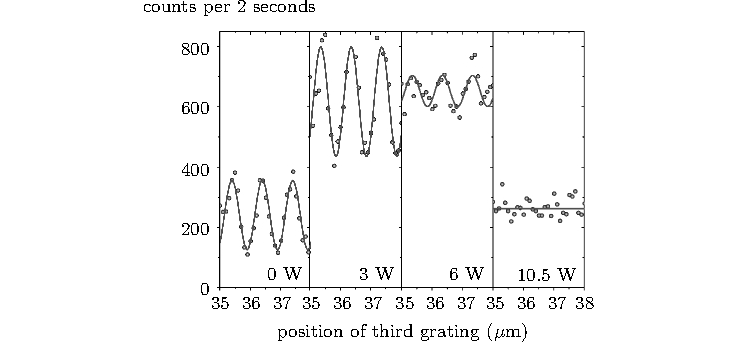
\includegraphics[width=.96\linewidth]{figures/ch06_fig13.pdf}
\caption{Hackermüllerら\cite{ref267}の実験で測定された、異なるレーザー加熱出力、したがって異なる分子平均温度における、$\mathrm C_{70}$分子の干渉模様。平均温度が上がるほど可視度が低下する。異なる加熱出力で全体の平均計数率が変わるのは、分子エネルギーによるイオン計数検出器の効率の変化と、加熱段階での電離・破砕効果による。Macmillan Publishers Ltdの許可を得て\cite{ref267}から転載：Nature, copyright 2004.}
\end{figure}
% 原文 p.267
\hypertarget{srcpage:267}{}\label{srcpage:267}
\begin{figure}[htbp]\centering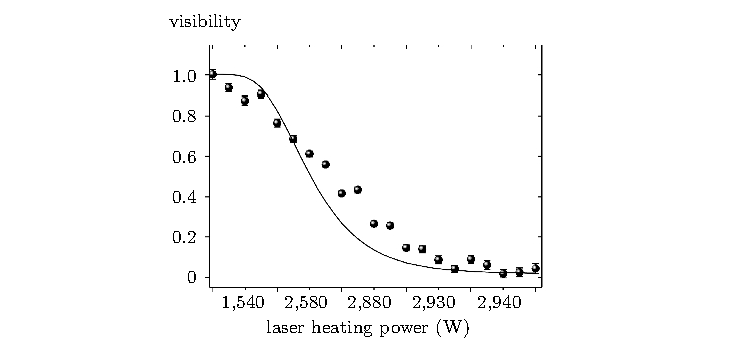
\includegraphics[width=.85\linewidth]{figures/ch06_fig14.pdf}
\caption{Hackermüllerら\cite{ref267}の実験における、レーザー加熱出力と平均分子温度の関数としての、$\mathrm C_{70}$干渉模様の可視度の減衰。円は実験データを表し、実線の理論予測によく一致する。Macmillan Publishers Ltdの許可を得て\cite{ref267}から転載：Nature, copyright 2004.}
\end{figure}
さらに詳しい実験の理論解析は、\cite{ref270,ref271}にある。

結果は、$\mathrm C_{70}$分子が約1000K以下なら、熱的デコヒーレンスは、干渉模様を観測できるほど弱いことを示す。約2000K以上では可視度を有意に低下させ、約3000Kで干渉模様は完全に消える。

これは次のように説明できる。放出光子が、$\mathrm C_{70}$分子の経路を分解できるだけの経路情報を伝えるには、その波長は、分子の異なる経路の隔たり、すなわち回折格子の異なるスリットの通過に対応する波束の極大間隔と、同程度でなければならない。この隔たりはスリット自体の間隔$d\approx1\,\mu\mathrm m$程度なので、熱的デコヒーレンスには、波長$\lambda\lesssim1\,\mu\mathrm m$の光子放出が必要である。分子がこの波長の光子を放出する有意な確率が現れるのは、2000Kを超える温度になってからだと分かる。約3000Kでは、典型的に、そのような光子を数個放出する。これが、干渉模様を完全に破壊するのに十分な経路情報を、環境へ移す。

\subsubsectionlink{バッキーボールを超えて}
$\mathrm C_{70}$分子の一粒子干渉縞が実験で観測された以上、自然な次の段階は、ますます大きな分子で、そのような量子効果を示すことである。
% 原文 p.268
\hypertarget{srcpage:268}{}\label{srcpage:268}
実際、Zeilingerのグループは、Hackermüllerらが2002年に報告した実験\cite{ref266}で、すでに次の一歩を踏み出した。$\mathrm C_{70}$用と同様の配置で、さらに重いフッ素化フラーレン$\mathrm C_{60}\mathrm F_{48}$（質量$m=1632\,\mathrm{amu}$、108原子）と、生体分子テトラフェニルポルフィリン$\mathrm C_{44}\mathrm H_{30}\mathrm N_4$（質量$m=614\,\mathrm{amu}$、幅2nm以上）の干渉模様が観測された。分子構造を図6.15、得られた干渉模様を図6.16に示す。これらの比較的重く複雑な分子でも、明確な干渉縞が観測され、可視度は理論予測によく一致した。
\begin{figure}[htbp]\centering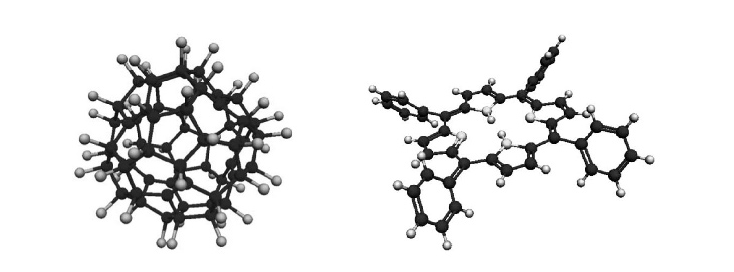
\includegraphics[width=.9\linewidth]{figures/ch06_fig15.pdf}
\caption{Hackermüllerら\cite{ref266}の干渉実験に用いられた、$\mathrm C_{60}\mathrm F_{48}$分子（左）と、生体分子テトラフェニルポルフィリン$\mathrm C_{44}\mathrm H_{30}\mathrm N_4$（右）の三次元構造。許可を得て\cite{ref266}から転載。Copyright 2003 by the American Physical Society.}
\end{figure}
\begin{figure}[htbp]\centering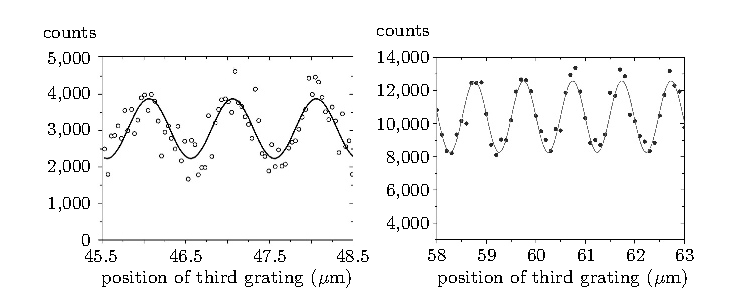
\includegraphics[width=.96\linewidth]{figures/ch06_fig16.pdf}
\caption{Hackermüllerら\cite{ref266}の実験で観測された、$\mathrm C_{60}\mathrm F_{48}$分子（左）と、生体分子テトラフェニルポルフィリン$\mathrm C_{44}\mathrm H_{30}\mathrm N_4$（右）の干渉縞。実線は当てはめた正弦曲線。許可を得て\cite{ref266}の図を改作。Copyright 2003 by the American Physical Society.}
\end{figure}

% 原文 p.269
\hypertarget{srcpage:269}{}\label{srcpage:269}
さらに大きい粒子、たとえばタンパク質やウイルスなどの生体分子\cite{ref268,ref272}、炭素質エアロゾル\cite{ref271}を使う干渉実験の実現可能性も、推測できる。そのような実験は、主に三つの要因で制限される。
\begin{enumerate}
\item 衝突デコヒーレンス。これらの分子の干渉縞を観測するには、装置内の真空が非常によくなければならない。背景気体密度の関数として干渉縞の可視度を記述するデコヒーレンス模型を使い、ライノウイルスの大きさに至るまでの、いくつかの生体分子について、干渉の観測に必要な真空の質が評価された\cite{ref268,ref272}（図6.17参照）。この評価は、現在の約3倍である、格子間隔1mの長いTalbot--Lau干渉計を使えることを仮定するが、これはまだ実験的に実現されていない。この設計なら、必要な低い背景気体密度は、現在の技術で達成できる範囲にある\cite{ref265,ref268}。
\item 熱的デコヒーレンス。大きな尺度では、これがますます重要になる。たとえば、Talbot--Lau干渉計とは異なる単純な二重スリット配置では、小さなウイルス（質量$5\times10^7\,\mathrm{amu}$）が、十分な可視度の干渉模様を示すには、約40Kまで冷却する必要があると評価された\cite{ref271}。そのような「冷たいウイルス」のビームを実験室で作るのは、明らかにかなり難しい。ゆえに、$\mathrm C_{70}$より大きい物体では、
% 原文 p.270
\hypertarget{srcpage:270}{}\label{srcpage:270}
衝突デコヒーレンスよりも、熱的デコヒーレンスの影響を弱める方が、実験的にははるかに難しくなるかもしれない\cite{ref271}。
\item 慣性力と振動による位相緩和。それ自体はデコヒーレンス効果ではないが、地球の質量と回転、回折格子の振動によって誘起される、重力的、回転的、音響的擾乱の雑音も、可視度へ影響する\cite{ref273}。これらは干渉縞の観測可能性を強く制限し得るので、実験者は、ここで述べたTalbot--Lau配置で、これらの雑音源を最小にすることに大きな注意を払っている。それでも、図6.17の粒子では、振動雑音が干渉観測の大きな障害になると予想される\cite{ref273}。現在利用できる配置では、その雑音は、衝突・熱的デコヒーレンス以上に、可視度を低下させる可能性が高い。
\end{enumerate}
\begin{figure}[htbp]\centering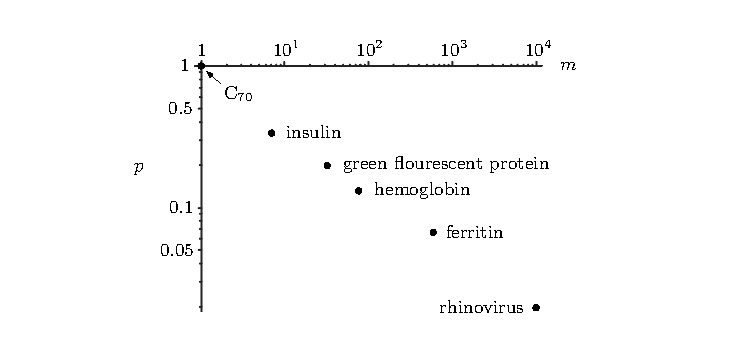
\includegraphics[width=.85\linewidth]{figures/ch06_fig17.pdf}
\caption{長いTalbot--Lau干渉計で、いくつかの生体分子の干渉縞を観測できる、背景気体の最大圧力$p$の評価。横軸は$\mathrm C_{70}$分子の質量を基準とする分子量$m$。縦軸の圧力は、$\mathrm C_{70}$の干渉観測に必要な圧力で規格化している。Hackermüllerら\cite{ref268}のデータから作図。}
\end{figure}

しかし、念頭に置くべき重要な点は、理論的デコヒーレンス模型を用い、干渉効果を観測する条件を精密に指定し定量化できることである。Copenhagen解釈が仮定するような、曖昧に定義された、量子領域と古典領域の基本的区分という仮定に、もはやとどまる必要はない。代わりに、対象分子を環境と相互作用する開いた量子系として扱うことで、干渉を観測するために何をすべきか、特定の実験設定でなぜ干渉縞が観測できないかを、理解できる。

$\mathrm C_{70}$分子は、周囲の粒子との衝突と熱放射の放出によるデコヒーレンスの、漸進的作用の観測を可能にする、ちょうどよい感受性を持つ。したがって、系を古典領域へ導くデコヒーレンスの、直接的で制御可能な影響を示す、これ以上分かりやすく直観的な実験を想像することは難しい。将来の干渉実験は、その限界をさらに巨視的領域へ押し進めると期待され、この分野の研究の進展を追うのは楽しみである。

\subsectionlink{SQUIDとその他の超伝導量子ビット}
それでは、超伝導量子二状態系、すなわち量子ビット系へ移ろう。過去10年、これらは巨視的なコヒーレンスとデコヒーレンスの実験研究で、中心的な役割を担うようになった。超伝導量子コンピューターの構成要素となる可能性も、その重要性を高めている\cite{ref274}。以下では、いわゆる超伝導量子干渉素子、略してSQUIDに焦点を当てる。Cooper対箱など、関連する他の型の超伝導量子ビット系にも触れる。

SQUIDは、さまざまな魅力的な量子効果を示せる巨視的量子系である。SQUIDでは、Bose凝縮した何十億もの電子対（以下参照）の状態が、
% 原文 p.271
\hypertarget{srcpage:271}{}\label{srcpage:271}
Schrödinger方程式に従って発展する、単一の集団的な巨視的変数で記述される。量子領域と、量子力学の限界の可能性を探索するSQUIDの潜在力は、早くから認識された。1980年、Leggett\cite{ref275}は、巨視的系で量子コヒーレントな振る舞いが可能であることを示すため、SQUIDの巨視的磁束状態の重ね合わせを含む思考実験を提案した。しかし、この提案が実験で成功するまでには、20年を要した\cite{ref276,ref277}。

\subsubsectionlink{超伝導と超電流}
超伝導現象は、1900年代初めにHeike Kamerlingh Onnesが初めて発見した。Onnesは液体Heで固体Hgを冷却し、絶対零度より数K高い温度で、Hgの電気抵抗が消えることを見いだした。1911年、「水銀の抵抗が消失する際の急激な速度について」という、適切な題名の論文\cite{ref278}で結果を公表した。2年後、この研究に対してNobel賞を授与された。しかし、微視的水準での理論的理解が得られたのは、1957年、Bardeen、Cooper、Schrieffer\cite{ref279}が、物質の結晶格子中のフォノンを介した相互引力により、逆向きのスピンを持つ電子が、いわゆるCooper対を形成することとして超伝導を説明してからであった。Cooper対は実効的にボソンとして働くため、フェルミオンである単一電子とは、著しく異なる性質を示せる。

Cooper対が、何の抵抗も受けずに物質を通過できるのは、なぜだろうか。各対は、第一励起状態からエネルギーギャップ$\Delta E$で隔てられた低エネルギー基底状態に対応することに注意しよう。結晶格子の熱振動エネルギーが$\Delta E$未満なら、格子は対の状態に遷移を誘起できず、対は格子との衝突で影響を受けない。これは、任意量のエネルギーを吸収・放出して散逸、したがって電気抵抗を生じさせる、単一の自由電子と対照的である。

超伝導の主要な特徴は、Cooper対がすべて同じ低エネルギー量子状態を取るため、多数の対が、対の集団的な重心運動を単一の巨視的波動関数で表す、無抵抗電流、すなわち「超電流」を形成できることである。量子力学の特異な特徴によって、そのような電流の流れには、外部電圧さえ必要ない。二つの超伝導物質の間に、非常に薄い絶縁障壁を入れるだけでよい。Cooper対はその障壁をトンネル通過し、電圧ゼロで超電流が流れる。この、実験的によく検証された純粋に量子力学的な現象は、いわゆるJosephson効果の、いくつかの形の一つであり、
% 原文 p.272
\hypertarget{srcpage:272}{}\label{srcpage:272}
障壁は対応してJosephson接合と呼ばれる（総説は\cite{ref280,ref281}参照）。

\subsubsectionlink{SQUIDの基本的物理}
SQUIDは、Josephson効果に直接基づく。超伝導物質の環に、一つ（rf-SQUID）または複数（dc-SQUID）のJosephson接合を入れたものである（図6.18）。本節では、単一接合のrf-SQUIDに焦点を当てる。接合を通るCooper対の量子トンネルによって、環に沿って超電流が流れ、SQUID環を貫く磁束が生じる。また、強度を調節できる外部磁場中にSQUIDを置き、追加の磁束$\Phi_{\mathrm{ext}}$を環へ与える。この外部磁束の目的は、後に説明する。

量子力学は、超電流を記述する波動関数が環に沿って連続であること、したがって波長の整数倍が環の周長に等しいことを要求する。環を一周する全位相変化は、$2\pi\Phi/\Phi_0$である。ここで$\Phi_0=h/(2e)$は、いわゆる磁束量子で、$e$は電子電荷である。$\Phi$は、超電流が作る磁束と外部磁場による$\Phi_{\mathrm{ext}}$からなる、環を貫く全捕捉磁束を表す。環にJosephson接合がなければ、波動関数の連続性は、条件
\begin{equation}\Phi/\Phi_0=k,\qquad k=1,2,\ldots\tag{6.31}\end{equation}
となる。しかしJosephson接合は、その物理的性質で完全に決まる、追加の位相シフト$\Delta\phi_{\mathrm J}$を導入する。位相連続性の完全な条件は、
\begin{equation}\Delta\phi_{\mathrm J}+2\pi\Phi/\Phi_0=2\pi k,\qquad k=1,2,\ldots .\tag{6.32}\end{equation}
\begin{figure}[htbp]\centering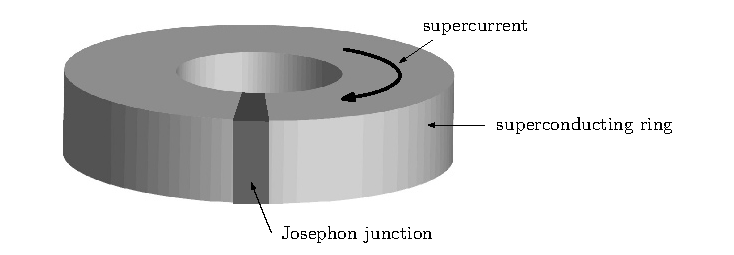
\includegraphics[width=.82\linewidth]{figures/ch06_fig18.pdf}
\caption{SQUIDの模式図。超伝導物質の環に一つまたは複数のJosephson接合を入れると、環に沿った無散逸の「超電流」が生じる。この超電流が、環を貫く磁束を作る。}
\end{figure}

% 原文 p.273
\hypertarget{srcpage:273}{}\label{srcpage:273}
$\Delta\phi_{\mathrm J}$と$\Phi_0$は固定されているので、(6.32)の唯一の自由パラメーターは全磁束$\Phi$である。したがってSQUIDでは、$10^9$個程度のCooper対という巨視的量の物質の動力学が、単一の巨視的座標$\Phi$の量子力学的発展によって、集団的に決定される。磁束が主要変数であるため、これらの素子はしばしば超伝導磁束量子ビットと呼ばれる。6.3.4節で述べるように、電荷や位相が主要変数となる、ほかの超伝導量子ビット系もある\cite{ref281}。

それでは、$\Phi$の動力学を論じよう。その発展は、次の形の有効Hamiltonianに従う。
\begin{equation}
H=\frac{P_\Phi^2}{2C}+U(\Phi)
=\frac{\hbar^2}{2C}\frac{\mathrm d^2}{\mathrm d\Phi^2}
+\left[\frac{(\Phi-\Phi_{\mathrm{ext}})^2}{2L}-\frac{I_c\Phi_0}{2\pi}\cos\left(2\pi\frac\Phi{\Phi_0}\right)\right].\tag{6.33}
\end{equation}
ここで$C$は全静電容量、$L$は環の自己インダクタンス、$I_c$はJosephson接合の臨界電流である。ここではこのHamiltonianの構造を導かない。関心のある読者は\cite{ref218}の導出を参照されたい。代わりに、それがどのような動力学を意味するのか、感覚をつかもう。

これは、ポテンシャル$U(\Phi)$中の、「質量」$C$を持つ仮想的「粒子」の運動を定めるHamiltonianと解釈できる。通常の正準変数である位置と運動量の役割は、ここでは全捕捉磁束$\Phi$と、その共役量$P_\Phi=-i\hbar\,\mathrm d/\mathrm d\Phi$が果たす。後者はしばしば全変位電流と呼ばれ、電荷の単位を持つ。実空間を動く粒子の運動エネルギーに相当するものは、ここでは静電エネルギーである。

外部磁場を調整し、誘起磁束$\Phi_{\mathrm{ext}}$をバイアス点$\Phi_{\mathrm{ext}}=\Phi_0/2$の近傍にすると、$U(\Phi)$は、傾いた一次元二重井戸ポテンシャルの形を取る（図6.19）。これが実験で関係する状況であり、以下ではこれを仮定する。傾きは$\Phi_{\mathrm{ext}}$によって決まり、$\Phi_{\mathrm{ext}}=\Phi_0/2$で、二重井戸は厳密に対称になる。この場合は後に詳しく論じる。したがって、外部印加磁場の強度で、ポテンシャルの形を変えられる。

大まかには、二つの井戸は、環を回る超電流の二方向、時計回りと反時計回りに対応する。各井戸は、接合による減衰が弱ければ、井戸間の障壁より十分低いところに局在する、Hamiltonian(6.33)のエネルギー固有状態$|k\rangle$をいくつか含む。こうして、環を回る古典的な持続時計回り電流、または反時計回り電流に、近似的に対応する、左井戸または右井戸のエネルギー固有状態の組を得る。

より正確には、波動関数$\psi_k(\Phi)\equiv\langle\Phi|k\rangle$は、局所的にs波型である。つまり、振幅は井戸の一方の底の周囲に狭いピークを持ち、
% 原文 p.274
\hypertarget{srcpage:274}{}\label{srcpage:274}
磁束空間での広がりが非常に小さい。したがって各$|k\rangle$は、全磁束$\Phi$の比較的狭い範囲に対応し、少なくとも十分小さな$k$では、磁束演算子の「ぼやけた」固有状態とみなせる。可能な離散磁束値は、連続性条件(6.32)で決まる。それゆえ$|k\rangle$は、しばしば「$k$フラクソイド状態」と呼ばれる。
\begin{figure}[htbp]\centering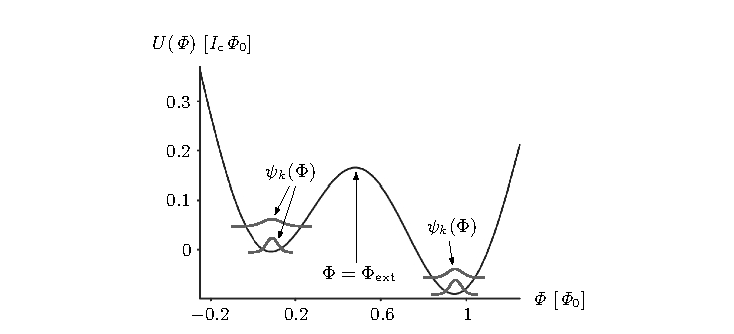
\includegraphics[width=.85\linewidth]{figures/ch06_fig19.pdf}
\caption{バイアス点$\Phi_{\mathrm{ext}}=\Phi_0/2$近傍の、SQUIDの有効二重井戸ポテンシャル$U(\Phi)$（単位$I_c\Phi_0$）。低いエネルギー固有状態$\psi_k(\Phi)\equiv\langle\Phi|k\rangle$は、各井戸の底近くによく局在し、したがって磁束演算子の近似的固有状態でもある。$\Phi$軸の単位は磁束量子$\Phi_0$で、$\Phi_{\mathrm{ext}}=3\Phi_0/5$とした。}
\end{figure}

古典的には、低い$k$フラクソイド状態$|k\rangle$のエネルギーは障壁高さ未満なので、二井戸を隔てる障壁を通過できない。しかし量子的には、井戸間の共鳴トンネルが起こり得る\cite{ref282,ref283}。たとえば放射場を加え、同じ井戸に局在する低い状態から高エネルギー状態へ系を励起すると、その状態は、その後、量子トンネルによって他方の井戸の、より低い、または等しいエネルギー準位へ減衰できる。これによって環を貫く磁束$\Phi$に巨視的変化が生じ、それが系の磁気モーメントの巨視的変化として観測できる。

通常SQUIDは、反対の井戸の底に局在する基底状態$|0\rangle$と第一励起状態$|1\rangle$が、より高い状態からエネルギー的によく分離するよう設計する。このとき、巨視的二状態系、すなわち量子ビットとして実効的に記述できる。基底には、超電流がそれぞれ確定した時計回りと反時計回りに流れる、二つの古典的持続電流状態$|\circlearrowright\rangle$、$|\circlearrowleft\rangle$を選ぶ。この二状態SQUIDの有効Hamiltonianは形式的に、
\begin{equation}\hat H=-\epsilon\hat\sigma_z-\Delta\hat\sigma_x.\tag{6.34}\end{equation}
% 原文 p.275
\hypertarget{srcpage:275}{}\label{srcpage:275}
と書ける。Pauliスピン演算子$\hat\sigma_z$の固有状態は$|\circlearrowright\rangle$、$|\circlearrowleft\rangle$であり、$2\epsilon=2I_p(\Phi_{\mathrm{ext}}-\Phi_0/2)$は、それらの非対称エネルギーを表す。$I_p\approx I_c$である。$\Delta$は二状態間のトンネル行列要素である。最低の二つのエネルギー固有状態$|0\rangle$、$|1\rangle$は、次の線形結合となる。
\begin{equation}|0\rangle=\cos\theta|\circlearrowright\rangle+\sin\theta|\circlearrowleft\rangle,\tag{6.35a}\end{equation}
\begin{equation}|1\rangle=-\sin\theta|\circlearrowright\rangle+\cos\theta|\circlearrowleft\rangle.\tag{6.35b}\end{equation}
ここで$\tan2\theta=\Delta/\epsilon$、エネルギーは$E_{0,1}=\mp\sqrt{\Delta^2+\epsilon^2}$である。したがって、$|0\rangle$と$|1\rangle$のエネルギー分裂は、$\Delta E=2E_1=2\sqrt{\Delta^2+\epsilon^2}$となる。バイアス点$\Phi_{\mathrm{ext}}=\Phi_0/2$から離れると、$\epsilon\gg\Delta$であり、$|\circlearrowright\rangle$、$|\circlearrowleft\rangle$は、それぞれゼロフラクソイド、1フラクソイドのエネルギー固有状態$|0\rangle$、$|1\rangle$と本質的に同一となる。これは上の議論に一致する。二状態$|0\rangle$、$|1\rangle$に対応する超電流の期待値は、$\pm I_p\cos2\theta$となることを示せる。正符号は時計回りを表す。

\subsubsectionlink{SQUIDの重ね合わせ状態とコヒーレント振動}
SQUIDがバイアス点$\Phi_{\mathrm{ext}}=\Phi_0/2$にあると何が起こるかを考えよう。二重井戸は対称になり、(6.34)で$\epsilon=0$となる。すなわち、左右の井戸のエネルギー準位がそろう。この場合、古典的には$|0\rangle$と$|1\rangle$の準位が交差し、縮退する。しかし量子的には、井戸間のトンネル障壁$\Delta$［(6.34)参照］が存続することで縮退が解ける。これが準位の「反発」をもたらし、反交差を生む（図6.20）。(6.35a)、(6.35b)では$\theta=\pi/4$なので、基底状態と第一励起状態は、持続電流状態の対称・反対称重ね合わせとなる。
\begin{equation}|0\rangle=\frac1{\sqrt2}(|\circlearrowright\rangle+|\circlearrowleft\rangle),\tag{6.36a}\end{equation}
\begin{equation}|1\rangle=\frac1{\sqrt2}(-|\circlearrowright\rangle+|\circlearrowleft\rangle).\tag{6.36b}\end{equation}
二つの新しい固有状態のエネルギー分裂$\Delta E$は、通常非常に小さく、接合の静電容量$C$だけで決まり、$\Delta E\propto e^{-\sqrt C}$とスケールする。

$|\circlearrowright\rangle$と$|\circlearrowleft\rangle$はそれぞれ左右の井戸に局在するので、重ね合わせ(6.36a)、(6.36b)は、二井戸にわたって非局在化している。この存在は、2000年、Friedmanら\cite{ref276}と、独立にvan der Walら\cite{ref277}が実験で確認した。Friedmanらの実験では、二状態はそれぞれ、何十億ものCooper対からなる、数$\mu\mathrm A$の逆方向の超電流に対応した。
% 原文 p.276
\hypertarget{srcpage:276}{}\label{srcpage:276}
これは、二電流の作る磁束に$\Phi_0/4$以上の巨視的差があることに当たり、局所磁気モーメントでは約$10^{10}\mu_{\mathrm B}$に等しい。$\mu_{\mathrm B}$はBohr磁子である。ゆえに、(6.36a)、(6.36b)は、20年前のLeggettの思考実験\cite{ref275}が描いたとおりの、巨視的に異なる状態のSchrödingerの猫型重ね合わせを表す。Friedmanらは、二状態間のエネルギー差$\Delta E$の静的分光測定という間接的方法で、存在を検証した。得られた$\Delta E$は、理論予測と極めてよく一致した。
\begin{figure}[htbp]\centering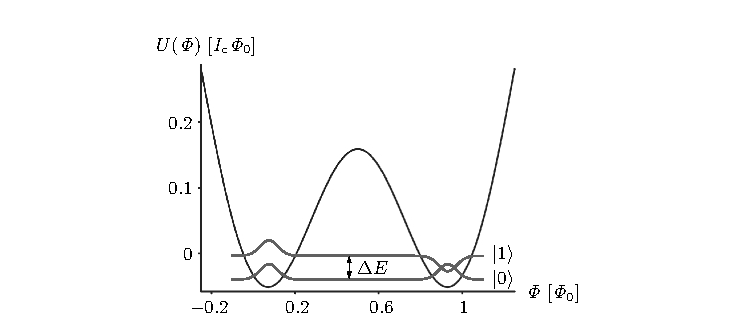
\includegraphics[width=.85\linewidth]{figures/ch06_fig20.pdf}
\caption{バイアス$\Phi_{\mathrm{ext}}=\Phi_0/2$でのSQUIDの有効ポテンシャル。この点で二重井戸は対称になる。トンネル障壁が井戸の準位交差を妨げ、非局在化した固有状態$|0\rangle=(|\circlearrowright\rangle+|\circlearrowleft\rangle)/\sqrt2$（新しい対称基底状態）、$|1\rangle=(-|\circlearrowright\rangle+|\circlearrowleft\rangle)/\sqrt2$（新しい反対称第一励起状態）の形成を介して、反交差が起こる。これらは「古典的」持続電流状態の重ね合わせである。存在は、分光測定\cite{ref276,ref277}とコヒーレントRabi振動の観測\cite{ref284,ref285}によって、実験的に確認された。}
\end{figure}

そのような重ね合わせの存在を示す別の方法は、持続電流状態間のコヒーレント振動を観測することである。これは6.1.1節のRabi型振動である。まず、SQUIDを貫く外部磁束を、縮退点$\Phi_{\mathrm{ext}}=\Phi_0/2$からわずかにずらし、エネルギー固有状態$|0\rangle$と$|1\rangle$を縮退近くにする。緩和させることで基底状態$|0\rangle$に初期化する。次に、二状態間の小さなエネルギー差$\Delta E$に周波数を合わせた、マイクロ波パルスを加える。Rabi振動の議論によれば、量子ビットは$|0\rangle$と$|1\rangle$の間、したがって持続電流状態間でも振動する［(6.35)参照］。
% 原文 p.277
\hypertarget{srcpage:277}{}\label{srcpage:277}
これは、巨視的超電流が環の時計回りと反時計回りの間で振動することとして現れる（図6.21）。振動はRabi周波数で起き、その周波数は量子ビットとマイクロ波場の結合強度で決まり、マイクロ波振幅に線形に依存する。したがって、SQUIDが二状態の各々にある相対確率は、パルスの振幅と長さに依存する［(6.8)参照］。

2003年、Chiorescuたち\cite{ref284}は、超伝導磁束量子ビットでこのRabi振動を実験的に示した。実験系は、三つのJosephson接合を入れた、$\mu\mathrm m$サイズの超伝導環からなる（図6.22）。単一接合のrf-SQUIDに比べ、三接合を使っても基本物理は大きく変わらないが、適切な調整が容易になる。量子ビットはさらに、Josephson接合を二つ持つdc-SQUIDに結合され、それが量子ビットの磁束を読む極めて高感度な装置として働く。

Chiorescuらは、与えられた長さと振幅のマイクロ波パルスを加え、次に、実験で利用できる観測量に対応する、持続電流基底$\{|\circlearrowright\rangle,|\circlearrowleft\rangle\}$で射影測定を行った。
\begin{figure}[htbp]\centering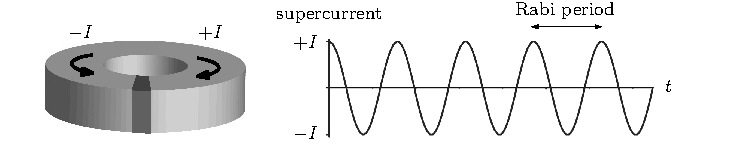
\includegraphics[width=.9\linewidth]{figures/ch06_fig21.pdf}
\caption{縮退点$\Phi_{\mathrm{ext}}=\Phi_0/2$の近くに調整したSQUIDの量子コヒーレントなトンネルは、巨視的超電流が時計回りと反時計回りの間でコヒーレントに振動することによって観測できる。}
\end{figure}
\begin{figure}[htbp]\centering
\includegraphics[width=.9\linewidth]{figures/ch06_fig22.pdf}
\caption{Chiorescuら\cite{ref284}の実験に使われた超伝導磁束量子ビット。右側の実際の量子ビットは、三つのJosephson接合を持つ小さな超伝導環である。白黒の矢印は持続電流の二方向を示す。量子ビットと一部を共有する、より大きい超伝導環に二接合を入れたSQUIDが、磁束の変化を検出する。許可を得て\cite{ref284}から転載。Copyright 2003 by AAAS.}
\end{figure}
% 原文 p.278
\hypertarget{srcpage:278}{}\label{srcpage:278}
この手順を数千回行い、たとえば超電流が時計回りとなる$|\circlearrowright\rangle$状態に、量子ビットを見いだす実験的確率を得た。マイクロ波振幅を固定し、パルス長を変えて繰り返すと、約150nsという驚くほど長い減衰時間を持つ、数百回の減衰Rabi振動を追跡できた（図6.23）。それが実際にRabi型の量子コヒーレント振動であると確認するため、研究者たちは、観測された周波数がマイクロ波振幅に線形比例することを検証した。これはRabi過程の主要な特徴である。別の連続読出し方式は、その後のIlichevら\cite{ref285}の実験で実現された。

Chiorescuら\cite{ref284}とIlichevら\cite{ref285}のRabi振動は、以前のFriedmanら\cite{ref276}とvan der Walら\cite{ref277}の分光結果とともに、巨視的に異なる超電流状態のコヒーレントな重ね合わせの存在を、印象的に示す。
\begin{figure}[htbp]\centering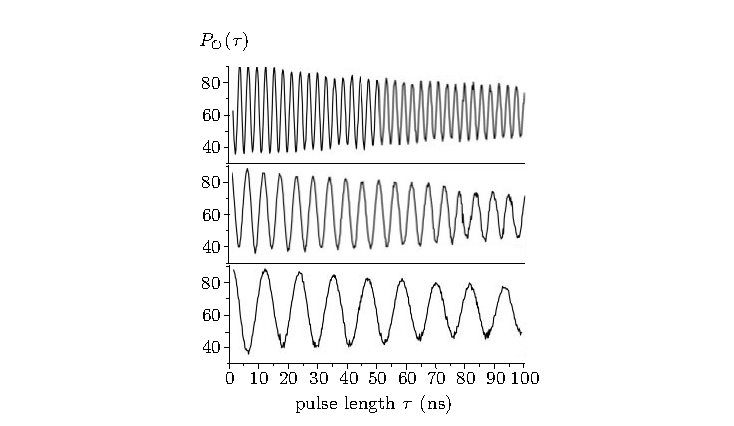
\includegraphics[width=.8\linewidth]{figures/ch06_fig23.pdf}
\caption{Chiorescuら\cite{ref284}の実験で観測された、超伝導磁束量子ビットの巨視的な逆方向超電流状態$|\circlearrowright\rangle$と$|\circlearrowleft\rangle$の間のRabi振動。これは二状態のコヒーレント重ね合わせを確認する。共鳴マイクロ波の三つの振幅の結果を示し、上から下へ振幅が小さくなる。縦軸は、特定の確定電流状態、たとえば$|\circlearrowright\rangle$に見いだされた実験の割合$P_{\circlearrowright}(\tau)$（\%）を、パルス長$\tau$の関数として示す。許可を得て\cite{ref284}の図を改作。Copyright 2003 by AAAS.}
\end{figure}
% 原文 p.279
\hypertarget{srcpage:279}{}\label{srcpage:279}
SQUIDは、この種の重ね合わせ状態の生成に特に適している。SQUID環を貫く捕捉磁束という、関係する巨視的変数を、Josephson接合の微視的なエネルギー差で制御できるからである\cite{ref286}。トンネル障壁の高さ$\Delta$は、環の大きさとは独立に、主として接合の性質で決まる。これは、達成可能な巨視的磁束状態の重ね合わせの「大きさ」が、異なりの程度そのもの、すなわち持続電流状態間の磁束差に、弱くしか依存しないことを意味する。

この特徴によって、ほかの実験で達成したものよりも、巨視的な異なりの程度がはるかに大きい「古典的」状態の重ね合わせを作れる。たとえば$\mathrm C_{70}$分子の物質波回折実験（6.2節）では、回折模様を観測するため、分子中の原子数$N$に伴って、回折格子の間隔を$1/\sqrt N$に従って減らす必要がある。したがって、この場合、ある大きさの分子の干渉模様を実験で作る能力は、分子の大きさ自体に応じて変わる。

\subsubsectionlink{デコヒーレンスを観測し定量化する}
振動する占有確率の包絡線の減衰（図6.23参照）から導かれる、Rabi振動の特徴的減衰時間は、持続電流重ね合わせ(6.36a)、(6.36b)に固有のデコヒーレンス時間尺度を、直ちに与えるわけではないことに注意が必要である。Rabi振動は、加えたマイクロ波パルスという外部駆動場によって誘起されるためである。しかしデコヒーレンス時間を測るには、制御されない環境と相互作用する量子ビットが、自由に、すなわち駆動なしで発展する間に、重ね合わせ成分間の相対位相情報が非局在化することを考えなければならない。

この目標は、Ramsey干渉法\cite{ref051}で達成できる。以下の手順は、2.2.2節で述べた「共鳴」Ramsey法の変形である。まず、量子ビットを縮退点$\Phi_{\mathrm{ext}}=\Phi_0/2$近くに設定し、再びエネルギー基底状態$|0\rangle$に初期化する。次に、二準位間の遷移周波数$\Delta E/(2\pi)$から$\delta f$だけ離調した、$\pi/2$マイクロ波パルスを加える。これにより$|0\rangle$と$|1\rangle$のコヒーレント重ね合わせへ変換し、時間$\tau$だけ自由に発展させる。この間、加えたマイクロ波周波数で回転する座標系では、相対位相が$2\pi(\delta f)\tau$だけ増す。その後、第二の非共鳴$\pi/2$パルスを加える。得られる重ね合わせでは、$|0\rangle$と$|1\rangle$の係数の大きさが、周波数$\delta f/2$で、遅延時間$\tau$に振動的に依存する。したがって、古典的な持続電流状態の占有確率は、
% 原文 p.280
\hypertarget{srcpage:280}{}\label{srcpage:280}
周波数$\delta f$で、$\tau$の関数として振動する。

実際には、量子ビットの自由発展時間$\tau$の間に、デコヒーレンスが二つのエネルギー状態、したがって持続電流状態間のコヒーレンスを減らすので、振動振幅は減衰すると予想する。2.2.2節で説明したように、完全にデコヒーレンスすると、占有確率が$\tau$に依存しない、持続電流状態の非コヒーレント混合へ至る。

遅延時間を増すと占有確率の振動がやがて消えることにより、デコヒーレンスの漸進的効果を観測し、定量化できる。Chiorescuら\cite{ref284}は、さまざまな遅延時間で、持続電流状態の関係する占有確率を測った。その減衰振動を追い、特徴的デコヒーレンス時間尺度を読み取った（図6.24）。

予想された、遅延時間への振動的依存性が見られる。振動周波数はマイクロ波の離調$\delta f$に一致し、Ramsey理論の予測と極めてよく一致した。包絡線の減衰から約20nsのデコヒーレンス時間を得た。これは、この実験で量子ビットが自由発展する間に、古典的な持続電流状態間の位相コヒーレンスが、環境によって失われる特徴的時間尺度である。

より最近の磁束量子ビット実験では、最大$4\,\mu\mathrm s$という、はるかに長いデコヒーレンス時間が観測された\cite{ref287}。この有望な結果は、超伝導量子ビットが固体量子計算素子の実現に適するかもしれないという期待を高めた（第7章参照）。制御パルスによるゲート操作は非常に速く、単一量子ビットゲート操作は約2nsで行える。
\begin{figure}[htbp]\centering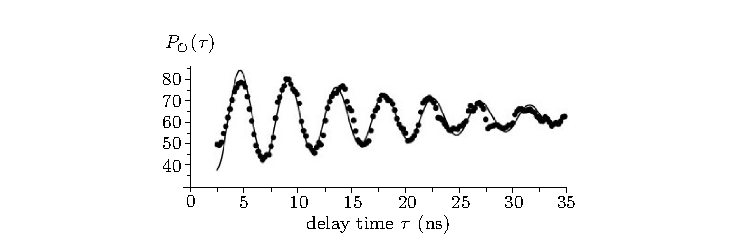
\includegraphics[width=.85\linewidth]{figures/ch06_fig24.pdf}
\caption{Chiorescuら\cite{ref284}の実験で観測された、超伝導磁束量子ビットへの二つの$\pi/2$パルスの遅延時間$\tau$に対する、占有確率$P_{\circlearrowright}(\tau)$の依存性。振動振幅の減衰は、系からの漸進的なコヒーレンスの喪失に対応する。許可を得て\cite{ref284}の図を改作。Copyright 2003 by AAAS.}
\end{figure}
% 原文 p.281
\hypertarget{srcpage:281}{}\label{srcpage:281}
したがって、コヒーレンスを相当失うまでに、1000回程度のゲート操作が可能かもしれない。しかし、単純な量子アルゴリズムにも必要な$O(100{,}000)$回には、まだかなり遠い。

SQUIDの磁束変数の代わりに、電荷または位相を主要変数とする超伝導素子でも、量子コヒーレント振動とデコヒーレンスが観測されている。一般に、超伝導電荷・位相素子の物理の形式的記述は、上述のSQUIDとよく似ている。

一般にCooper対箱として知られる超伝導電荷量子ビットは、貯蔵庫からJosephson接合を通ってCooper対がトンネルできる、小さな超伝導「島」からなる。二つの量子ビット基底は、少なくとも一つのCooper対だけ異なる、島の二つの電荷状態に対応する。Cooper対箱は、電荷状態間のRabi振動を実験観測できた、最初の超伝導量子ビット系であり、1999年にNakamura、Pashkin、Tsai\cite{ref288}が達成した。2002年にはVionら\cite{ref289}が、$0.5\,\mu\mathrm s$のデコヒーレンス時間を持つ、数千回のコヒーレント振動を報告した。

Rabi型のコヒーレント振動は、位相量子ビットでも観測された。位相量子ビットはrf-SQUIDと同様、単一のJosephson接合を含む。ただし、環を貫く磁束の代わりに、主要変数は接合電極間の位相差である。Yuら\cite{ref290}は、巨視的に異なる位相状態間のRabi振動を測り、最大数$\mu\mathrm s$のデコヒーレンス時間を得た。Martinisら\cite{ref291}も、同様の結果を報告した。

現在の実験的証拠（たとえば\cite{ref291,ref292}参照）は、超伝導量子ビットのデコヒーレンスの主な源が、予想されそうな、環・接合系を制御する外部回路との相互作用ではなく、Josephson接合と超伝導体の内部欠陥の存在であることを示す。これらの欠陥は、しばしば有効二準位系として模型化できる。5.1.2節で触れたように、超伝導系などの低温系のデコヒーレンスと散逸が、主にこのような内部二準位系によることは、しばらく前から知られている\cite{ref199,ref200}。量子ビット自体が二準位系なので、そのデコヒーレンスの理論的記述に適切な模型は、5.4節のスピン・スピン型である可能性が高い\cite{ref199}。

たとえばMartinisら\cite{ref292}は、絶縁体のバルクとJosephson接合の両方にある二準位状態による誘電損失が生む、超伝導位相量子ビットのデコヒーレンス研究へ、この模型を適用した。理論研究から得た知見は、著しく改善された実験構造へ、成功裏に反映された。ほかの理論研究は、電流バイアスJosephson接合を制御するバイアス電流の揺らぎなど、雑音過程の影響を調べている\cite{ref293}。しかし、
% 原文 p.282
\hypertarget{srcpage:282}{}\label{srcpage:282}
2.12節の一般的議論（7.3節も参照）に照らすと、そのような雑音による集団の位相緩和と、環境とのもつれが生む「真の」デコヒーレンスを、明瞭に区別することが重要である。局所測定統計という現象論的視点では、両者が同様の結果を生むとしても、同じではない。
\subsectionlink{その他の実験領域}
前の各節では、中間的尺度および巨視的尺度で異なる状態の重ね合わせを生成・検出し、その漸進的デコヒーレンスを観測できた実験を述べた。これらでは、実験室で観測された量子から古典への現象を、デコヒーレンスが定性的・定量的に説明した。

同じように、ただし別の視点から、ある実験で重ね合わせ状態を生成・観測できない原因を理解するうえでも、デコヒーレンスは役立つ。本節では、現在までに得られたものよりも、さらに大きい非古典的重ね合わせを、将来生成・観測するための有望な候補となる、二つの実験領域を述べる。見るように、それらで重ね合わせの生成・観測がこれほど難しい理由を、デコヒーレンスによって定性的・定量的に記述できる。また、実験手順の改善方法を示唆し、実験室で望ましい重ね合わせを作る目標に、さらに近づくことも可能にする。

\subsubsectionlink{Bose--Einstein凝縮体におけるデコヒーレンス}
Bose--Einstein凝縮は、巨視的数の原子が、ある実験では最大$O(10^7)$個まで、量子相転移を起こし、すべての原子が個別性を失って同一量子状態を占める凝縮体となる、量子力学的現象である。したがって凝縮体は、位相を持つ単一の量子力学的$N$粒子波動関数で完全に記述できる。この位相は実験で調べられる。たとえば二つの凝縮体を重ねると、両者の位相差による干渉模様が観測される\cite{ref294,ref296,ref297,ref298,ref299}（図6.25）。最近は、単一凝縮体をコヒーレントに分割し、その後再結合して干渉縞を観測する干渉計も作れるようになった\cite{ref295}（同じく図6.25参照）。

このような量子的性質の実証の成功にもかかわらず、粒子数が巨視的に区別される状態の重ね合わせに、凝縮体を準備する実験は、いくつかの有望な理論提案\cite{ref300,ref301,ref302,ref303,ref304,ref305,ref306}があるにもかかわらず、これまで失敗している。
% 原文 p.283
\hypertarget{srcpage:283}{}\label{srcpage:283}
しかし、関係するデコヒーレンス機構を考慮すれば、この失敗は定性的にも定量的にもよく理解できる。凝縮体の重ね合わせ状態では、デコヒーレンスは主に、凝縮原子と非凝縮原子の間の、弾性・非弾性散乱によることが分かる。
\begin{figure}[htbp]\centering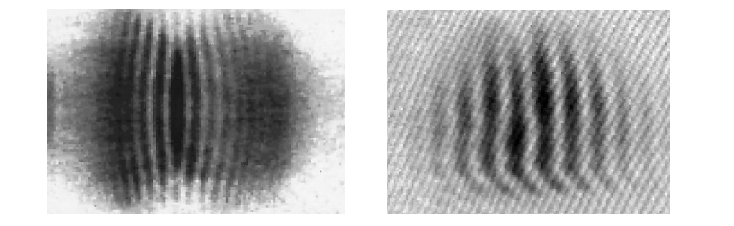
\includegraphics[width=.94\linewidth]{figures/ch06_fig25.pdf}
\caption{Bose--Einstein凝縮体の原子気体密度の干渉模様。左：独立な二凝縮体を重ねたときの、位相差による模様。許可を得て\cite{ref294}から転載。Copyright 1997 by AAAS. 右：凝縮体の「二重スリット」干渉計で得られた干渉縞。単一凝縮体をコヒーレントに分割し、通常の二重スリットの役割を模擬した後、再結合した。許可を得て\cite{ref295}から転載。Copyright 2004 by the American Physical Society.}
\end{figure}

この散乱過程の詳細な模型が作られ（たとえば\cite{ref102}参照）、凝縮体の大きさなどの主要実験パラメーターの関数として、デコヒーレンス時間尺度の現実的予測が得られる。また、これらの模型の知見は、巧妙な実験設計によってデコヒーレンスを最小にする具体的提案を生んだ。改善案には、デコヒーレンスを誘起する非凝縮原子の熱的雲を、より速く蒸発させる、修正した凝縮体トラップ\cite{ref102}、粒子数差状態ではなく相対位相状態の巨視的重ね合わせを作り、環境の選ぶ指針基底を考慮してデコヒーレンスを最小にすること\cite{ref303}、熱的雲の実効的大きさを減らす能動的な環境設計（7.5.3節）\cite{ref102}、重ね合わせ状態のより速い生成\cite{ref306}などがある。各提案は、特定の実験配置に関係する、さまざまなデコヒーレンス機構の分析から導かれる。配置が与えられると、模型は量子・古典境界の位置と、望ましい猫状態を実現するため、その境界を押し進めるには何ができ、何をすべきかを教える。

% 原文 p.284
\hypertarget{srcpage:284}{}\label{srcpage:284}
\subsubsectionlink{量子電気機械系におけるデコヒーレンス}
量子電気機械系、略してQEMSは、さらに大きい非古典的重ね合わせを生成する可能性を持つ、多彩な実験の仲間に、比較的最近加わったものである\cite{ref307}（入門は\cite{ref308,ref309}も参照）。QEMSには、デコヒーレンスと散逸の「振動子・スピン模型」との関連で、5.4.2節ですでに触れた。何十億もの原子が、空間中のよく区別できる二位置の重ね合わせにある、真に機械的な「Schrödingerの子猫」を示すために、QEMSは非常に有望である。この分野の急速な実験進展から、今後数年で、量子から古典への移行の探索で中心的な役割を果たす可能性が高い。

QEMSは、近年のナノテクノロジーの革命の成果である。主要部分は、シリコンなどの結晶材料から作る、小型の両端固定梁または片持ち梁で、典型寸法はnmから$\mu\mathrm m$程度である（図6.26）。梁は小さな機械的共振器として働く。短時間適切な駆動力を加えると、振動運動を始める。

寸法が極めて小さいため、機械系であることを考えると、振動周波数は驚くほど高くできる。最近の実験では、マイクロ波領域の1GHzまで達成した\cite{ref311}。また、共振器の散逸は比較的弱くでき、振幅が有意に減少するまでに、数万回自由振動する。運動は電子トランスデューサーで検出し、対応する電気信号へ変換して読み出す。
\begin{figure}[htbp]\centering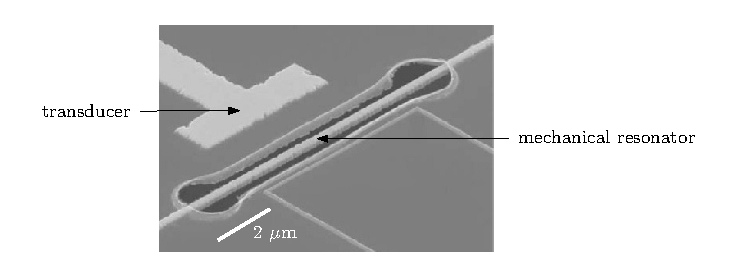
\includegraphics[width=.94\linewidth]{figures/ch06_fig26.pdf}
\caption{Cornell UniversityのKeith Schwabの研究室\cite{ref310}で作られた、量子電気機械系の実験的実現。幅200nm、長さ$8\,\mu\mathrm m$の梁が、固有周波数19.7MHzのナノ機械共振器として働く。電子トランスデューサーで、梁の振動を電気信号へ変換する。許可を得て\cite{ref310}から転載。Copyright 2004 by AAAS.}
\end{figure}
% 原文 p.285
\hypertarget{srcpage:285}{}\label{srcpage:285}
注目すべきことに、共振器の大部分の自由度は、QEMSの典型的動作温度であるmKという低温で「凍結」されるか、トランスデューサーへの結合が無視できる。したがって多くの場合、巨視的共振器は、梁の最低の基本曲げモードに対応する、単一の量子力学的調和振動子として実効的に扱える。QEMSのナノ機械共振器は、何十億もの原子からなり、多数の内部欠陥や不完全さで乱された、巨視的機械物体である。それにもかかわらず、これから述べるように、明確に量子力学的な効果を示せる。

QEMSの主要な特徴は、空間変位への極めて高い感度である。重要な量は、位置検出の量子限界を表す、調和振動子の量子零点変位の不確定性$\Delta x_{\mathrm{zp}}$である。現在実験室で作られるナノ機械共振器では、わずか0.1pm程度である\cite{ref307}。それでも最近の実験では、たとえば図6.26のQEMSを用い、$\Delta x_{\mathrm{zp}}$の数倍に至るまで空間変位を分解できた\cite{ref310}。したがって、量子限界での位置測定という目標に非常に近づいている。

\subsubsectionlink*{QEMSによる機械的「Schrödingerの子猫」の生成法}
研究者たちは、共振器を二つの異なる空間変位のコヒーレント重ね合わせに置き、その漸進的デコヒーレンスを観測する可能性も考えている。特に面白いのは、QEMSが、たとえば超伝導量子ビット（6.3節）やBose--Einstein凝縮体（6.4.1節）よりも、日常世界の物体にはるかに近い、純粋な機械構造であることだ。実現すれば、それは、巨視的で「粗い」通常物質の機械物体が、二つの異なる位置にある重ね合わせを表す。現時点では、そのような重ね合わせはまだ実験室で実現されていないが、具体的提案\cite{ref312}があり、関係するデコヒーレンス・散逸機構の理論研究も進んでいる\cite{ref242,ref313,ref314,ref315}。巨視的距離だけ離れた複数の共振器をもつれさせる考えも、理論的に調べられた\cite{ref316}。量子コンピューターの機械的量子ビットとして使う可能性も、考えられる\cite{ref317}。

Armour、Blencowe、Schwab\cite{ref312}の提案した、QEMSの空間的重ね合わせの生成法を簡単に概説しよう（\cite{ref307}も参照）。基本的考えは、基底状態$|0\rangle$、$|1\rangle$が共振器の異なる二変位へ結合し、しかもそれらの重ね合わせへ比較的容易に準備できる、二状態量子系を使うことである。
% 原文 p.286
\hypertarget{srcpage:286}{}\label{srcpage:286}
\cite{ref312}ではCooper対箱を選んだ（6.3.4節参照）。二基底状態は、超伝導島上の異なる電荷値に対応する。箱と片持ち梁の静電相互作用は、箱が$|0\rangle$か$|1\rangle$かに応じて、共振器に二つの異なる変位を与える（図6.27）。対応する重心位置状態を、$|P_0\rangle$、$|P_1\rangle$と書こう。

箱を$(|0\rangle+|1\rangle)/\sqrt2$の重ね合わせに準備する。\cite{ref312}が示したように、特定の制御パルス列を箱へ加えると、もつれた箱・共振器の重ね合わせ
\begin{equation}|\Psi\rangle=\frac1{\sqrt2}(|0\rangle|P_0\rangle+|1\rangle|P_1\rangle)\tag{6.37}\end{equation}
が得られる。二重心状態の空間的隔たりが十分巨視的なら、Schrödingerの猫型の状態を生成したことになる。共振器が猫の役割を果たし、箱は元の設定の不安定な原子に対応する。

重ね合わせ(6.37)の存在は、Ramsey干渉法（2.2.2節）で確認できる。ある遅延時間後に、Cooper対箱へ追加の制御パルスを加えると、もつれた状態が変換され、
% 原文 p.287
\hypertarget{srcpage:287}{}\label{srcpage:287}
箱を$|0\rangle$または$|1\rangle$に見いだす確率が、遅延時間に振動的に依存する。この依存性は、箱・共振器系が成分状態の古典混合にあるなら現れない。6.3.4節で論じたように、Ramsey法は特徴的なデコヒーレンス時間の情報も与える。
\begin{figure}[htbp]\centering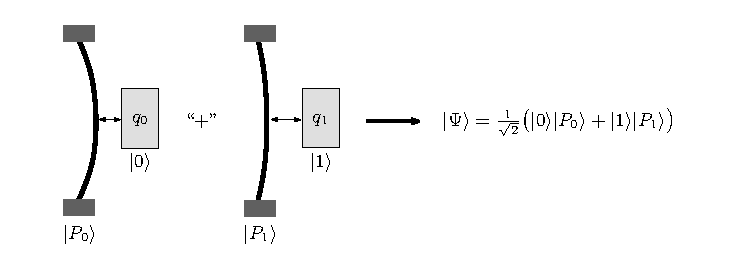
\includegraphics[width=.96\linewidth]{figures/ch06_fig27.pdf}
\caption{Armour、Blencowe、Schwab\cite{ref312}が提案した、ナノ機械共振器の二つの異なる位置の重ね合わせを生成する方法。箱の超伝導島の異なる電荷$q_0$、$q_1$に対応する基底状態$|0\rangle$、$|1\rangle$で記述されるCooper対箱を、共振器へ静電結合する。箱をコヒーレント重ね合わせ$(|0\rangle+|1\rangle)/\sqrt2$に準備し、適切な制御パルス列を加えると、もつれた箱・共振器の重ね合わせ$(|0\rangle|P_0\rangle+|1\rangle|P_1\rangle)/\sqrt2$が得られる。$|P_0\rangle$、$|P_1\rangle$は、共振器の識別できる二つの重心位置に対応する。}
\end{figure}

\subsubsectionlink*{QEMSにおけるデコヒーレンス}
上述の生成法の実用的な実現可能性を評価するには、その重ね合わせに影響するデコヒーレンスの主な源を理解することが重要である。まず、Cooper対箱自体も、もちろんデコヒーレンスを受ける。しかし、6.3.4節で述べたように、$\mu\mathrm s$領域の比較的長い時間は実験的に達成可能である\cite{ref289}。したがって、共振器自体の環境相互作用によるデコヒーレンスに焦点を当てられる。

興味深いことに、現在の実験的証拠\cite{ref318,ref319}、および初期の結果（たとえば\cite{ref320,ref321}）は、QEMSの主な散逸源、したがってデコヒーレンス源も、共振器の最低の基本曲げモードと、共振器内の局在した欠陥との相互作用かもしれないことを示す。これらの欠陥は有効二準位系で、電荷トラップ、不純物原子、弾性中心、共振器表面の結晶構造の乱れによる未結合手など、さまざまな物理的実現を取る。

現時点では、欠陥の基礎にある正確な物理的詳細や、曲げモードとの相互作用は、実験でも理論でも、まだ十分理解されていない。上述の空間的重ね合わせはまだ実現されていないため、QEMSのデコヒーレンスの直接実験データは存在しない。しかし、近年の実験は、散逸の特徴的性質について、貴重な情報を与えた\cite{ref318,ref319}。

散逸には一般にデコヒーレンスが伴うが、その逆は成り立たないので、こうした測定から、デコヒーレンスの性質についても知見を得られる。たとえば散逸データから、欠陥で構成される環境の有効スペクトル密度を取り出せるかもしれない。共振器と欠陥の相互作用の適切な模型があれば、それを使って、関係するデコヒーレンス係数と動力学を計算できる。そして、上述の重ね合わせの特徴的デコヒーレンス率を評価し、生成法の実現可能性を検討できる。ゆえに、QEMSの散逸とデコヒーレンスの現実的模型の開発が、主要な目標の一つとなる\cite{ref242,ref314,ref315}。それは理論的理解を高めるだけでなく、重ね合わせの実験的実現を前進させ、QEMSの実装全般の改善も示唆する。

% 原文 p.288
\hypertarget{srcpage:288}{}\label{srcpage:288}
Armour、Blencowe、Schwabは、最初の提案\cite{ref312}で、5.2節のよく研究された量子Brown運動模型を用い、空間的な箱・共振器重ね合わせ(6.37)のデコヒーレンス時間を評価した。中心調和振動子が基本曲げモードを表し、ほかの調和振動子からなる環境へ弱く結合する。しかし上述のように、mK温度のナノ機械共振器の環境は、欠陥を表す二準位系の集まりとして記述する方が、より現実的かもしれない。これらを量子スピン$1/2$粒子として模型化すれば、振動子・スピン模型が得られる。その弱結合マスター方程式は、5.4.2節で導いた［(5.198)参照］。

しかし、この模型の減衰率の温度依存性［(5.200)参照］は、散逸率が温度とともに増加するというQEMSの実験データ\cite{ref318,ref319}と一致しない。この不一致は、欠陥の少なくとも一部を、さらに別の、デコヒーレンスと散逸を生む環境に強く結合した、スピン$1/2$粒子として扱うべきことを示す（図6.28）。この環境は、スピンのトンネルを非コヒーレントにし、緩和も生じさせ、古典的二準位揺動子に似た欠陥動力学を誘起する。スピン浴から過剰エネルギーを吸収することで、その飽和を防ぐ。したがって、より現実的な模型は、独立なスピン・ボソン模型、すなわち振動子浴と相互作用するスピンを複数個、中心調和振動子へ結合したものかもしれない。この模型の最初の研究は、ごく最近行われた\cite{ref242}。このようにQEMSは、異なるデコヒーレンス・散逸模型を、実験で区別し検証する機会を与える。
\begin{figure}[htbp]\centering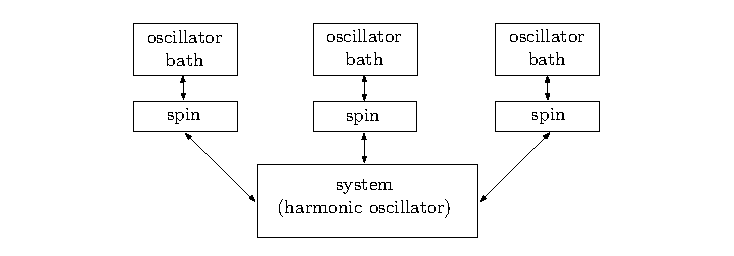
\includegraphics[width=.86\linewidth]{figures/ch06_fig28.pdf}
\caption{QEMSのデコヒーレンスと散逸の、考えられる模型。中心系は、ナノ機械共振器の基本曲げモードを表す調和振動子からなる。これは、スピン$1/2$粒子として模型化した二準位欠陥の集合と相互作用する。さらに各スピンは、散逸的な振動子浴へ結合し、その浴が、そうしなければ容易に飽和するスピン環境から、エネルギーを吸収する。}
\end{figure}

% 原文 p.289
\hypertarget{srcpage:289}{}\label{srcpage:289}
\subsectionlink{展望}
Schrödingerが1935年に猫の逆説を初めて描いたとき、それを純粋な思考実験、経験する巨視的世界へ量子力学を適用したときに生じる、明らかに「不合理な」帰結の例と考えた。しかし、過去数年、比較的小さいとはいえ、それでも巨視的なSchrödingerの猫を、実験室で育て、観測することに、大きな進展があった。本章では、数十個の光子を含む、巨視的に区別できる二状態の重ね合わせの生成（6.1節）、重い$\mathrm C_{70}$分子の干渉模様の観測（6.2節）、逆方向に流れる二つの$\mu\mathrm A$電流の重ね合わせの存在の検証（6.3節）を達成した実験を述べた。

各実験で研究者は、デコヒーレンスの漸進的作用、すなわち環境との相互作用により、重ね合わせがやがて観測できなくなる様子も、明示的に測定できた。こうして、量子から古典への移行の滑らかさを、明瞭に見た。量子状態を古典状態へ不連続に変換するような、固定された障壁は、量子領域と古典領域の間にない。系と環境の相互作用を操作することで、移行の動力学と時間尺度を直接変えられる。

したがって、本章の実験は、デコヒーレンスの範囲が、周囲の巨視的物体の、実効的に瞬時の「局在化」を指すだけよりも、はるかに広いことを示す。デコヒーレンスは、実効的古典性の出現を、漸進的で制御可能な過程として説明する。それは実験室で直接観測・検証でき、標準的量子力学の形式で厳密に理論記述できる。

ここでは、理論と実験の相互作用が非常に密接である。デコヒーレンス時間尺度や、その動力学のほかの性質の測定によって、模型を実験室で直接試せる。そして、模型がどの程度現実的で、物理的に適切かを学ぶ。一方、模型は、既存と将来の実験について貴重な情報を与える。ある配置で、どの段階の「巨視性」で量子から古典への移行を予想すべきか、あるパラメーターの組でどの種の「Schrödingerの子猫」を生成・観測できそうか、さらに「猫らしい」重ね合わせを作るため、実験をどう改善できるかを教える。本章では、理論的方式で提案された特定の重ね合わせの生成を、まだ達成していない二領域、Bose--Einstein凝縮（6.4.1節）と量子電気機械系（6.4.2節）を述べた。それでも、測定データとデコヒーレンス模型を組み合わせれば、望ましい重ね合わせを「見る」のを妨げる、物理的に関係する機構を同定でき、
% 原文 p.290
\hypertarget{srcpage:290}{}\label{srcpage:290}
有害な効果を弱める方法が示唆される。

自然に生じる問いは、巨視的に異なる状態の重ね合わせの実験が、将来どこへ向かうのか、その結果が量子力学の理解や、量子コンピューターなどの大規模量子系の構築に、どのような含意を持つか、ということである。答えは多いので、主要な点を少しだけ挙げよう。

まず、これまで調べた尺度では、既存の実験的証拠は、重ね合わせ原理の根本的限界を示していない。環境との望ましくない相互作用を最小にする適切な設計で、デコヒーレンスを十分制御できる限り、その限界は精密な定量解析が可能だが、「古典的」状態のどのような数の重ね合わせも、生成・観測できるように見える。

したがって、今後数年、巨視的に異なる状態の重ね合わせの、達成可能な「大きさ」の限界を、さらに押し進める多くの実験を見ることになる、といってよい。近いうちに、ウイルスのような、さらに大きい生体分子の干渉模様を観測し、凝縮体やナノ機械共振器の重ね合わせを実現し、超伝導量子ビットのデコヒーレンス時間を飛躍的に延ばせるかもしれない。このような実験は、重ね合わせ原理が破れる可能性を探し続けることによっても動機づけられる。しかし、デコヒーレンスは局所観測者からは見かけの破れを生じさせるので、十分にそれを遮蔽しながら、ユニタリー発展からのずれを誘起する機構には適度に敏感な実験を設計するのは、今後も非常に難しいだろう（8.4節および\cite{ref286,ref322}参照）。

ますます異なる巨視的状態の重ね合わせを生成・観測できることは、その重ね合わせ自体や、デコヒーレンスと量子力学一般に関わる、根本的な解釈上の問いを解かないことを、強調する必要がある。量子状態（2.1節）、特に重ね合わせ状態（2.2.1節）の適切な解釈と物理的意味の問題は、2.2.2節のStern--Gerlach実験のような、微視的設定ですでに明らかである。近年の巨視的重ね合わせ実験は、Schrödingerの猫型の直観に反する色合いを加えるかもしれないが、解釈の根本問題を解きも、深めもしない。

特に、環境を含む全体の量子状態でコヒーレンスが持続することをどう理解するか、したがって、デコヒーレンスの密度行列記述から生じる量子状態の非真正混合を、基礎にある何らかの量子的実在へどう適切に関係づけるかは、基礎論上の論争であり続ける。
% 原文 p.291
\hypertarget{srcpage:291}{}\label{srcpage:291}
ここで論じた型の実験は、少なくとも「実在の本性」についての先入観へ、さらに挑むことで、議論を今後も明るく照らすだろう。純粋にユニタリーな動力学からのずれを、実験が決定的に示す、あるいは排除できるようになれば、量子力学と量子的実在の構造について、新たな知見を得るか、得ざるを得なくなるかもしれない。しかし現在は、本章の驚くべき実験的成果を踏まえても、解釈の問題は残り続ける。



\clearpage
\setcounter{section}{6}
\setcounter{footnote}{0}
\sectionlink{デコヒーレンスと量子計算}
% 原文 p.293
\hypertarget{srcpage:293}{}\label{srcpage:293}
量子情報理論と量子計算は、過去10年のあいだに急速に大きな関心を集め、理論的・実験的研究の焦点の一つになった。量子情報理論は、量子力学の多くの基本概念を、新しい視点から捉える。また、将来量子コンピューターを構築する可能性を含め、量子技術とその応用に関する提案を促してもきた。有用なアルゴリズムを実行する量子コンピューターは、実験的実現にはまだほど遠いが、多くの考えが検討され、量子コンピューターの基本的な構成要素となりうる部品のいくつかは、すでに実験室で開発されている。

同時に、量子情報理論と量子計算の研究は、デコヒーレンス効果の研究と制御への関心を飛躍的に高めた。基礎的な観点から見ると、環境とのvon Neumann型測定相互作用としてのデコヒーレンスの基本的な形式的記述（2.5.1節と2.6.3節参照）は、条件付き量子力学の形式を使って、量子情報理論の言葉で表し直せる\cite{ref016,ref323}（後の7.4.1節も参照）。さらに、本書の前の章でもすでに、デコヒーレンスと（かなり曖昧な）「情報」の概念との結び付きに触れた。具体的には、環境とのもつれが、どの状態にあるかという情報を運び去り、デコヒーレンスをもたらす仕組みの議論で、この結び付きを示した（2.6節参照）。実用的な観点からは、どのような量子コンピューターも、その動作は量子コヒーレンスを維持する能力に決定的に依存する。デコヒーレンスは計算に誤りを生じさせるため、量子コンピューターの実現にとって最大の障害である。

本章では、量子計算においてデコヒーレンスが果たす役割を概説する。7.1節では、量子計算と古典計算の主要な違い、および量子計算の基礎にある中心的な考えの歴史的発展を含め、量子計算の基本的側面を振り返る。7.2節では、量子コンピューターのどのような実現でも核心となる、デコヒーレンスと制御可能性のあいだのトレードオフを論じる。続く7.3節では、量子計算という主題に即して、デコヒーレンスと雑音の違いについて、さらにいくつか述べる（2.12節も参照）。7.4節では、いわゆる量子誤り訂正によって、量子コンピューターで有害なデコヒーレンスの影響を軽減する方法を説明する。
% 原文 p.294
\hypertarget{srcpage:294}{}\label{srcpage:294}
最後に7.5節では、2.8.1節で導入したデコヒーレンスのない（すなわちポインター）部分空間の概念を用いる量子計算を論じる。量子情報理論と量子計算全般についてさらに学びたい読者は、たとえばNielsenとChuangの著書\cite{ref056}に多くの内容を見いだすだろう。

\subsectionlink{量子計算の概観}
今日買ったコンピューターが、ほんの数年後には救いようもなく時代遅れになることは、誰もが知っている。過去数十年間にコンピューターが高速化した速さは、驚異的としかいいようがない。それに伴い、コンピューターのプロセッサーを構成する回路の複雑さ（たとえば、チップ当たりのトランジスター数で測る）は、急速に増え続けている。読者は、回路の複雑さがおよそ2年ごとに倍になるという、Mooreの有名な「法則」を聞いたことがあるかもしれない。この予測は、これまで驚くほど正確であった。

この結果、1970年代と1980年代の少数の研究者たちは、ある時点でチップ上の個々の処理構造（たとえばトランジスター）が、量子効果が重要になる原子スケールに達するはずだと気付いた。\footnote{Moore自身は1997年の講演で、これが2017年ごろに起こると予測した\cite{ref324}。}そこから、こうした量子効果を実際に利用して計算能力を高められるのか、という考察へ導かれた。さらに大胆にいえば、量子力学の原理を巧みに使うことに、その能力が特に依存するようなコンピューターを作れるだろうか。

\subsubsectionlink{量子計算の能力}
本質的に量子的なコンピューターが、なぜ通常の（「古典的な」）コンピューターよりはるかに強力になりうるのか、少し考えてみよう。古典コンピューターは、論理ビットという基本単位で情報を符号化する。その値は「0」か「1」のいずれかを取る。量子情報理論の主要な標語は、「情報は必然的に物理的である」というものである（この洞察をおそらく最初に強調したのはLandauer\cite{ref325}であった）。紙上の鉛筆の線であれ、トランジスター中の電子の存在であれ、情報はつねに何らかの物理系によって符号化されなければならない。したがって、情報の符号化自体が物理法則に従う。

そこで、ビット値「0」と「1」に対応する二状態を取りえ、そのため1ビットの情報を符号化できる物理系を考えよう。コンピューターの構成要素が小さくなるという先の議論に沿えば、この系は、古典的に区別可能で、古典ビットの二つの値に対応する二つの基底状態$|0\rangle$と$|1\rangle$をもつ量子系であってよい。
% 原文 p.295
\hypertarget{srcpage:295}{}\label{srcpage:295}
このような「量子ビット」の系は、2.10節と第5章ですでに論じた。原理的には、実効的に二次元の状態空間をもつ任意の量子系を量子ビットとして用いられる。その例は、二つの偏光自由度をもつ光子、イオンや原子核のスピン、および二つの支配的なエネルギー準位をもつ原子である。これらの物理的実現のいくつかは、後の7.1.5節で説明する。

量子力学によれば、この系は、少なくとも原理的には（すなわち$\{|0\rangle,|1\rangle\}$基底でのデコヒーレンスを無視できれば）、コヒーレントな重ね合わせ
\begin{equation}|\psi\rangle=\alpha|0\rangle+\beta|1\rangle\tag{7.1}\end{equation}
にもなりうる。大ざっぱにいえば、値が0か1のいずれかである古典ビットとは異なり、量子ビットは二つの論理ビット0と1を同時に符号化できることを意味する。係数$\alpha$と$\beta$の選び方は無限にあるため、一つの量子ビットが取りうる状態は、古典ビットの二状態に対して無限に存在する。与えられた状態$|\psi\rangle$にある一つの量子ビットは、二つの実数を符号化できるが、古典ビットは一つの2進数字しか表さない。これは、$|\psi\rangle$がつねに
\begin{equation}|\psi\rangle=|\alpha|e^{i\phi_0}|0\rangle+|\beta|e^{i\phi_1}|1\rangle\tag{7.2}\end{equation}
と書けることからわかる。物理的に関係のない全体の位相因子を無視すれば、これは
\begin{equation}|\psi\rangle=|\alpha||0\rangle+|\beta|e^{i(\phi_1-\phi_0)}|1\rangle\tag{7.3}\end{equation}
と表される。規格化条件$|\langle\psi|\psi\rangle|^2=1$を用いると、さらに
\begin{equation}|\psi\rangle=\cos\left(\frac{\theta}{2}\right)|0\rangle+\sin\left(\frac{\theta}{2}\right)e^{i\phi}|1\rangle\tag{7.4}\end{equation}
と書き直せる。ここで$\phi\equiv\phi_1-\phi_0$であり、角$\theta$を適切に選ぶ（$0\leq\theta\leq\pi$）。式(7.4)は、このような状態をBloch球の描像によって見やすく可視化できる形である（図7.1参照）。こうして、無限に存在する単一量子ビット状態のどれも、二つの実数（ここでは角$\theta$と$\phi$）を符号化することを示した。

今度は、系が$N$個の量子ビットから構成されるとしよう。この系のHilbert空間は、単一量子ビットのHilbert空間$\mathcal H_i$（$1\leq i\leq N$）のテンソル積$\mathcal H=\mathcal H_1\otimes\mathcal H_2\otimes\cdots\otimes\mathcal H_N$で与えられるため、次元は$2^N$である。したがって、互いに直交する$2^N$個の基底状態が存在する。通常、これらは第$i$量子ビット（$1\leq i\leq N$）の元の単一量子ビット基底状態$|0\rangle_i$と$|1\rangle_i$の積状態に選ばれる。
\begin{equation}\begin{aligned}|00\cdots0\rangle&\equiv|0\rangle_1|0\rangle_2\cdots|0\rangle_N,\\|00\cdots1\rangle&\equiv|0\rangle_1|0\rangle_2\cdots|1\rangle_N,\\&\ \vdots\\|11\cdots1\rangle&\equiv|1\rangle_1|1\rangle_2\cdots|1\rangle_N.\end{aligned}\tag{7.5}\end{equation}
% 原文 p.296
\hypertarget{srcpage:296}{}\label{srcpage:296}
\begin{figure}[htbp]\centering
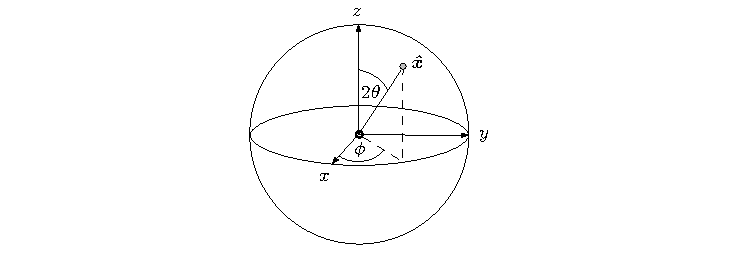
\includegraphics[width=.42\linewidth]{figures/ch07_fig01.pdf}
\caption{量子ビットの状態を、$\mathbb R^3$内の単位球であるBloch球上の点として幾何学的に表したもの。任意の量子ビット状態は二つの実パラメーター$\theta$と$\phi$で記述できる［式(7.4)参照］。ここで$2\theta$と$\phi$は、よく知られた球座標の役割を果たす。すなわち、状態(7.4)は単位ベクトル$\hat{\bm x}=(\sin2\theta\cos\phi,\sin2\theta\sin\phi,\cos2\theta)$によって表される。}
\end{figure}
この基底を、$N$量子ビット系の計算基底と呼ぶ。任意の$N$量子ビット状態は、$2^N\times2^N$の密度行列でも記述できる。この行列を対角化すれば、対角成分には$2^N$個の実数値（密度演算子の固有基底における占有数を表す）があるため、この状態は$2^N$個の独立な実数を同時に符号化できることがわかる。これに対して、$N$個の古典ビットが符号化するのは、長さ$N$の2進文字列にすぎない。ここに量子コンピューターの第一の利点がある。量子ビットの配列の記憶容量は古典ビットの配列より指数関数的に大きく、一つの量子ビットは、無限に存在するコヒーレントな重ね合わせ状態(7.1)のどれにもなれる。

第二の利点は、古典コンピューターと量子コンピューターが情報を処理する仕方の違いに関係する。古典コンピューターでは、一度に一つか二つのビットに作用する論理ゲート（AND、NOT、XORなど）を適用する。量子の場合、ゲートの実行は、$N$量子ビット系のHilbert空間に作用するユニタリー変換$\hat U$の適用に対応する。\footnote{量子計算には別の方法もあり、初めに高度にもつれた状態（いわゆるクラスター状態）へ準備した量子ビット系に対する、時間順に並んだ射影測定の列として、計算全体を進める\cite{ref326,ref327,ref328}。このような測定に基づく（またはクラスター状態）量子計算は、ユニタリーなゲート操作に基づく従来の量子計算と、まったく同じ計算課題を実行できることが示せる。言い換えれば、測定に基づく量子コンピューターは、「標準的な」量子コンピューターと同じく普遍的である。量子測定の非ユニタリー性からは、任意の（したがってユニタリーなものも含む）量子力学的時間発展のシミュレーションとは両立しないと直観的に考えそうであるため、これは注目すべき結果である。クラスター状態量子計算は、高度にもつれた$N$量子ビット状態を準備し、それを時間とともに生じるデコヒーレンスに対して十分頑健に保つ必要があるため、一般的なデコヒーレンスの性質は、ゲートに基づく量子計算と似ていると予想される。クラスター状態量子計算のわかりやすい入門として、文献\cite{ref329}を参照されたい。}

% 原文 p.297
\hypertarget{srcpage:297}{}\label{srcpage:297}
ここで鍵になるのは、このような変換$\hat U$は、一つの量子ビットにしか作用しない場合でも、$N$量子ビット系の大域的状態を変えうることである。たとえば最大にもつれた状態では、一つの量子ビットに加えたユニタリー操作が、一般に、全$N$量子ビットの大域的状態を変える。したがって、その操作は、全量子ビット系の$2^N$個の基底状態すべてに同時に作用する。簡単な例として、Bell型(2.7a)の二量子ビットもつれ状態
\begin{equation}|\Phi^+\rangle=\frac{1}{\sqrt2}(|00\rangle+|11\rangle)\tag{7.6}\end{equation}
に、第一の量子ビットだけに作用するユニタリー変換$\hat U$、たとえば
\begin{equation}\hat U=(-|0\rangle\langle1|+|1\rangle\langle0|)_1\otimes\hat I_2\tag{7.7}\end{equation}
を施すとしよう。変換後の状態は
\begin{equation}\hat U|\Phi^+\rangle=\frac{1}{\sqrt2}(|10\rangle-|01\rangle)\tag{7.8}\end{equation}
となる。この特徴は、もつれた多粒子状態の、非局所的で全体論的な性質の帰結と見ることができる。ここでも、古典的な状況と対比される。古典的には同じ操作を$2^N$回行うか、一つの古典論理ゲートをそれぞれ適用する$2^N$個の「プロセッサー」を並列に働かせる必要がある。\footnote{この観察との類推で、量子コンピューターは大規模な「量子並列性」を示すとよくいわれる（この特徴は、Zurekが早い時期に「量子Monte Carlo」の名で指摘した\cite{ref330}）。ただし、この用語は慎重に解釈すべきである。並列性は、多くの独立した過程が並列に実行されるという印象を与えるが、量子の場合には実際には、一つの量子力学的な「全体」（すなわち大域的な量子状態）が、一つの操作（量子ゲート）を受けると考えるべきである。}実際には、一度に一つか二つの量子ビットに作用する量子ゲートだけを考えればよい。一量子ビットゲートと二量子ビットゲートの、ある特定の集合が、任意の量子計算を実行するのに十分であることを示せるからである\cite{ref056,ref331,ref332,ref333,ref334}。多量子ビットゲートを物理的に実現するために必要な、三つ以上の量子ビットのあいだの相互作用を作り出すことは、実際には難しいので、これは非常に有用な結果である。

\subsubsectionlink{量子コンピューターの読み出し}
古典コンピューターでは、全ビットの最終値を単に読み出すだけで、計算結果を得る。これは、コンピューターの状態を変えることなく、いつでも行える。
% 原文 p.298
\hypertarget{srcpage:298}{}\label{srcpage:298}
量子計算で対応する手続きは、計算の最後に、いくつかの（あるいはすべての）量子ビットについて、選んだ基底で射影測定を行うことである。量子測定の標準理論によれば、これは$N$量子ビット系の大域的状態を、測定する基底の一状態へ収縮させ、個々に測定された各量子ビットと他の量子ビットのあいだに存在するもつれを破壊する。古典的な場合との主要な違いは、量子力学の測定が確率的であるという事実に関係する。すなわち、同一に準備した$N$量子ビット系の集まりに同じ量子ゲート列を適用しても、測定結果は一般に系ごとに異なる。指定できるのは、測定の際に系がある状態として見いだされる確率だけである（2.1節参照）。

同一の量子計算を繰り返した最後に、一般には単一の一貫した結果を得られないため、この事実は量子計算を本質的に無用なものにするように見えるかもしれない。したがって量子コンピューターは通常、少なくとも場合によっては、計算課題に正しい答えを与えない。しかし幸い、多くの状況では、ある出力が本当に正しい結果かどうかを確認するのは比較的容易である。たとえば、量子コンピューター上で整数を因数分解する有名なアルゴリズム（後の7.1.4節参照）は、つねに正しい答えを与えるわけではない。しかし、整数を素数に分解した結果が正しいかどうかは簡単に確認できるので、量子コンピューターの誤った結果は、単に人の手で捨てればよい。最終的に測定された状態が正しい解に対応する確率が十分に高ければ（たとえば、正解を得るために必要な実行回数が問題の大きさとともに指数関数的に増えなければ）、それでも量子コンピューターの能力を有利に利用したことになる。

\subsubsectionlink{物理系のシミュレーション}
ここで次の問いを考えよう。古典コンピューターは、少なくとも原理的には、量子系をつねにシミュレートできるだろうか。\footnote{自明なことを述べる恐れはあるが、量子コンピューターも任意の古典コンピューターをシミュレートできることを指摘しておく。そのためには、各量子ビットがどの時刻にも$|0\rangle$か$|1\rangle$のいずれかで記述され、それらの重ね合わせにはならないように、状態を準備して量子ゲートを適用すればよい。この点は、量子計算におけるデコヒーレンスの役割についての後の議論に直接関係する。デコヒーレンスは、$N$量子ビット系の計算基底状態(7.5)のコヒーレントな重ね合わせを破壊する傾向があり、そのため量子ビットを実効的に古典論理ビットのレジスターへと変える。すると量子コンピューターは「量子的な能力」を失う。古典コンピューターと同じ機能は実行できるが、それ以上のことはできなくなる。}たとえば、$N$量子ビット系の量子状態を$2^N\times2^N$の行列で表し、ゲート操作を表す別の$2^N\times2^N$行列を適用することで、その時間発展を模倣できると考えるかもしれない。しかし、注意すべき点が二つある。
% 原文 p.299
\hypertarget{srcpage:299}{}\label{srcpage:299}
第一に、すでに見たように、この方法は$N$が大きくなると、計算量が手に負えなくなる。行列の大きさと行列演算の回数（したがって記憶容量と処理能力への要求）が、$N$の増加とともに指数関数的に膨れ上がるためである。そのため、大きな量子系（言い換えれば、量子アルゴリズム）を古典コンピューターでシミュレートするのは、あらゆる実用上の目的に対して不可能になる。第二に、より基礎的な観点からは、Bellの定理\cite{ref030}によって、相関がBell不等式を破るような、離れた二つの相関した系を準備できる古典的機構は存在しないことが示される。したがって、このような（EPR/Bell型の）相関は、量子世界と量子計算に特有の特徴である\cite{ref335,ref336}。

量子系をどう効率よくシミュレートするかという問題は、量子計算研究の根源にある。Feynman\cite{ref335}は1982年の重要な論文で、自然界の他の任意の（量子）系の物理的振る舞いを効率よく模倣できる量子系を構築する問題を考察した。量子コンピューターも必然的に物理系でなければならないので、そのような系は普遍的な模倣装置であるだけでなく、普遍量子コンピューターでもある。Feynmanは、この普遍的な模倣装置を、最近接相互作用をもつスピンの格子によって模型化した。よく知られるように、彼は、この模型が原理的には、有限次元のHilbert空間で記述できる他の任意の量子系をシミュレートできることを示した。これは基礎的に重要な、真に画期的な発見であった。しかし、Feynmanの模型にはまだ欠点があった。新しい計算課題ごとに、一般にはスピン間相互作用の形と強さを変える必要があったのである。この要求を実際に実現するのは明らかに難しく、Feynmanは、支配するHamiltonianを利用者が自由に選ぶための物理的機構を指定しなかった。

したがって次の段階は、固定されたHamiltonian（すなわち特定の物理的構成）に基づき、量子コンピューターに施す操作を変えるだけで、任意の問題を解ける普遍量子コンピューターを考案することであった。これは、David Deutschが1985年の重要な論文\cite{ref337}で達成した。Deutschは、二状態系の集まりに基づく模型を使った。これらの系を合わせた状態に、ユニタリー変換の小さな集合（先に述べた「量子ゲート」）を適用すると、原理的には任意のユニタリーな時間発展を実現し、したがって任意の物理系をシミュレートできることを示した。可能な時間発展の広い一群に対しては、この量子コンピューターは効率よくも動作する\cite{ref338}。すなわち、ある時間発展を実現するのに必要な計算手順の数は、入力の大きさ（Deutschの模型では二状態系の数）に対して、指数関数より遅く増える。他の（ほとんど）どの物理系も効率よくシミュレートできることにより、Deutschの提案は、（ほとんど）普遍的な量子コンピューターの最初の設計図となった。

% 原文 p.300
\hypertarget{srcpage:300}{}\label{srcpage:300}
\subsubsectionlink{有名な量子アルゴリズムの例}
Deutschの論文に続く数年間、研究者たちは、古典コンピューターに対する量子コンピューターの優位性を示す計算課題を探すことに忙しかった\cite{ref339,ref340,ref341,ref342,ref343}。初期の試みはあまり実りがなかったが、1994年にPeter Shor\cite{ref344,ref345}が、因数分解問題（与えられた整数を素数の積へ分解する課題）を、多項式時間だけで解ける量子アルゴリズムを提示した。具体的には、$N$桁の数に対して$O(N^2)$の時間である。これに対して、古典コンピューターで因数分解問題を解くには、指数時間が必要だと広く考えられている（厳密に証明されてはいない）。したがって、相当に大きな数については、古典コンピューターでこの課題を達成するのは、本質的に不可能である。Shorの発見の重要性は、潜在的な実用的応用よりもむしろ、そのアルゴリズムが、Steane\cite{ref336}の言葉でいう「量子力学の本質の何かを定義するうえで、Bell不等式と同様の概念的役割」を果たすという点にあるのかもしれない。

量子計算分野を取り巻く初期から現在までの関心の多くは、Shorのアルゴリズムを根源とするといってよい。それ以来、量子コンピューターの能力を示す新しいアルゴリズムの発見は、比較的ゆっくりと進んできた（文献\cite{ref339,ref342}参照）。Shorのアルゴリズム以後で、おそらく最も重要な発見は、Groverの探索アルゴリズムである\cite{ref346,ref347}。このアルゴリズムは、非常に効率のよいデータベース探索を可能にする。構造をまったくもたない$N$項目のリストから、ある特定の項目を$O(\sqrt N)$の手順で見つけられる。これに対して、古典コンピューターでは、特定の項目を見つけるために、平均してリストの半分を調べる（すなわち$N/2$回の手順を行う）必要があるため、この課題には$N$程度の手順を要する。したがって、Groverのアルゴリズムを実行する量子コンピューターは、どのような古典コンピューターよりも$O(\sqrt N)$倍速い。

\subsubsectionlink{量子コンピューターの物理的実現}
上の量子計算への導入は、意図的にかなり抽象的なものにとどめた。ユニタリー変換（ゲート）の適用によってコヒーレントに操作できる、量子ビットの集まりが手元にあると、単に仮定しただけである。量子ビットの物理的性質も、こうしたゲート操作を実際にどう実行するかも指定しなかった。実際、量子コンピューターの原型（コヒーレントに制御できる、少数の量子ビットを含む系）の実験的実現に関する研究領域は広大であり、この急速に進む分野を概観しようとすることは、本書の範囲を完全に超える。

読者が最初の見当を得るために、表7.1では、将来、本格的な量子コンピューターへ発展する可能性のある、量子ビットと制御機構（ゲートと測定を実現する）の物理的実現の例をいくつか挙げる。各技術には長所と短所があり、それらは一般に、次の7.2節で論じる、デコヒーレンスと制御可能性のあいだの基本的なトレードオフに帰着する。
% 原文 p.301
\hypertarget{srcpage:301}{}\label{srcpage:301}
\begin{table}[htbp]\centering\small
\caption{量子ビット系と量子ビット制御の物理的実現の例。}
\begin{tabular}{lll}\hline
方式&量子ビットの実現&量子ビットの制御\\\hline
光学&光子&光学媒質\\
イオントラップ&捕獲イオン&レーザー光\\
共振器QED&二準位原子&レーザー光\\
NMR&核スピン&磁場\\
固体&結合した量子ドット&点接触\\
&超伝導トンネル接合&接合のバイアス電流\\\hline
\end{tabular}\end{table}
表7.1の構成要素を用いる現在の実験では、少数の量子ビットしかコヒーレントに制御できていない。有用な量子アルゴリズムを実行するには、はるかに多くの量子ビットが必要であり、したがって、これらの実験は量子コンピューターの実用的実現から、なお大きく隔たっている。

\subsectionlink{量子コンピューターにおけるデコヒーレンスと制御可能性}
すでにいくつかの箇所で示唆したように、量子コンピューターの能力は、計算基底状態(7.5)の非局所的でコヒーレントな重ね合わせの存在に由来する。これらの計算基底状態は、個々の量子ビットの基底状態$|0\rangle$と$|1\rangle$の積状態である（量子コンピューターを制御する何らかの装置によって操作し、測定できるよう、両状態は十分に区別可能でなければならない）。したがって量子計算は、中間的または巨視的に異なる状態の重ね合わせに基づいており、それらは通常、デコヒーレンスにきわめて敏感である。デコヒーレンスは量子コンピューターの最大の敵であり、量子コンピューターの実現に関する研究の、すべてとはいわなくても多くは、デコヒーレンスをいかに制御し、最小化し、「取り消す」かという問題をめぐって進められてきたといってよい。

量子コンピューターのデコヒーレンス問題に対処するため、量子ビットをあらゆる環境との相互作用からできるだけ遮蔽すれば十分だと提案したくなるかもしれない。確かに、量子ビットを周囲から孤立させれば、デコヒーレンスは最小になる。しかし、この方策は量子コンピューターの機能も損なう。すでに見たように、量子計算は、量子ビットにユニタリー操作の列を適用することで実行される。物理的には、そのようなゲート操作は、量子ビット系と外部装置との何らかの相互作用に対応する。その相互作用の具体的な物理的形態は、量子コンピューターの個別の実現方法によって異なる（表7.1参照）。
% 原文 p.302
\hypertarget{srcpage:302}{}\label{srcpage:302}
量子ゲートを確実に実行するためには、量子ビットと制御装置の相互作用が十分に強くなければならない。

したがって、相反する二つの要求に直面する。一方では、望ましくない環境との相互作用を最小にし、量子ビットの重ね合わせ状態を保護するために、量子ビットを孤立させたい。他方では、巨視的装置との制御された相互作用により、量子ビットを操作し（状態準備とゲート操作の形で）、読み出せるように、系を十分に開いておく必要がある。すると、こうした量子ビットと装置の相互作用は、一般に装置とのもつれによって量子ビットにデコヒーレンスを生じさせ、装置の古典的雑音（揺らぎ）によってさらに擾乱が加わる。

したがって、量子コンピューターの設計という困難な課題は、両方の要求を均衡させて満たすことにある。環境によるデコヒーレンス率が非常に低くても、まともに操作できない量子コンピューターは、よく制御できても、環境との相互作用が強すぎて装置が直ちに古典コンピューターへと劣化してしまう量子コンピューターと同じく、役に立たないことは明らかである。要するに、量子ビットは、環境のある構成要素（すなわち装置）とは強く相互作用し、残りの部分（量子ビットを取り囲む、制御されない周囲）とは相互作用しないことが求められる。

たとえば光量子計算は、光子を物理的量子ビットとして使い、偏光の二つの異なる向きで計算基底状態を表す。光子は電荷をもたず、通常、互いに、また物質とも弱くしか相互作用しないため、デコヒーレンスに比較的鈍感である。通常の線形光学媒質では、光子は互いにまったく相互作用せず（非線形媒質でも、相互作用はきわめて弱い）、そのため、一対の光子をもつれさせる二量子ビットゲート操作をどう実行するかという問題が生じる。このジレンマから抜け出す可能な方法として、有名なKnill--Laflamme--Milburn方式\cite{ref348}が提案されている。この方式は、線形光学、単一光子状態、射影測定だけを用いて、二つの光子量子ビットをもつれさせる。しかし今度は、この方式自体が、光量子コンピューターの構築を可能にするために克服すべき新たな課題を生む。同様に、原子核内の単一スピンとして実現した量子ビットは、デコヒーレンス時間が長いが、制御と測定が非常に難しい。

\subsectionlink{デコヒーレンスと古典的揺らぎ}
2.12節で論じたように、デコヒーレンスは、古典的な対応物のない、明確に量子力学的な効果として理解すべきである。これに対して量子計算の文献では、「デコヒーレンス」という用語が、古典的な揺らぎや不完全さによる擾乱を含め、量子ビットに影響するあらゆる過程を指す、もっと大まかな意味で使われていることが多い。
% 原文 p.303
\hypertarget{srcpage:303}{}\label{srcpage:303}
量子計算におけるこのような古典的雑音の源には、イオントラップ内の量子ビットに入射するレーザー光の強度\cite{ref349}と持続時間\cite{ref350}の揺らぎ、NMR量子計算での磁場の不均一性\cite{ref351}、超伝導量子ビットでのバイアス揺らぎ\cite{ref293}などがある。

現象論的にも形式的にも、このような古典的過程が量子ビットに及ぼす影響は、環境とのもつれの効果と同様に、すなわち「量子ビット誤り」によって記述できる（後の7.4.2節参照）。したがって純粋に実用的な観点では、一方にある環境とのもつれを生む相互作用によるデコヒーレンスと、他方にある古典的雑音による（アンサンブル平均での）位相コヒーレンスの喪失との区別は、関係しないかもしれず、しばしば明示されない。量子誤り訂正（7.4節参照）の分野も、誤り訂正方式が量子ビット誤りの物理的起源に依存しないため、古典的雑音と量子デコヒーレンスの区別をさらに曖昧にしている。

さらに2.12節で述べたように、環境とのもつれによる位相コヒーレンスの喪失は、ときに、系を乱す古典的揺らぎ、すなわち系の自己Hamiltonianにある時間依存項を加えることで模擬される。この方法は、たとえば、イオントラップ量子コンピューターの量子ビットの位相コヒーレンスに、揺らぐパラメーターが及ぼす影響の理論的研究\cite{ref349,ref352}と実験的研究\cite{ref125,ref353}で実行された。理論面では、SchneiderとMilburnが、量子ビットを制御するレーザー光の位相と強度のランダムな揺らぎ\cite{ref349}、およびイオンを閉じ込めるトラップのパラメーターの揺らぎによる「デコヒーレンス」を調べた。NISTのグループによる実験\cite{ref125,ref353}では、トラップされたイオンのSchrödingerの猫状態（コヒーレント状態および数固有状態の重ね合わせ）の減衰に対する、異なる種類の熱浴の影響を、調和トラップの極小位置やトラップ周波数などのパラメーターをランダムに揺らがせることで、実験的に模擬した。

2.12節ですでに論じたように、ここで鍵となるのは、環境の影響をこのように古典的雑音として模型化すると、コヒーレンスの減衰はアンサンブルにしか、すなわち、その雑音過程の多数の個別の実現についての平均としてしか現れないことである。系は外部環境に結合していないので、雑音過程の個々の実現では系の力学は完全にユニタリーであり、系からコヒーレンスが失われているはずはない。これに対して、系が環境の自由度ともつれる場合、適切な逆変換を加えてデコヒーレンスの効果を反転させるのに十分な情報を得るには、少なくとも系との相互作用の前後に、環境に対して一対の測定を行う必要がある。さらにNISTの実験\cite{ref125}で示されたように、これらの測定は、デコヒーレンスを「取り消す」のに、つねに十分な手続きになるわけではない（文献\cite{ref016}のIV.C節も参照）。
% 原文 p.304
\hypertarget{srcpage:304}{}\label{srcpage:304}
したがって、この実験は、古典的雑音と環境によるデコヒーレンスの主要な類似点と相違点のいくつかを、見事に示している。

もちろん、これは古典的雑音が量子計算で重要でないという意味ではない。逆に、実験的実現での揺らぎと不完全さに起因する雑音は、環境とのもつれが生じさせるデコヒーレンスの効果と同じくらい重要かもしれない。以下でも「デコヒーレンス」は環境とのもつれの帰結を記述する用語として用いるが、より一般的な「量子ビット誤り」は、特に断らないかぎり、古典的雑音によるか環境とのもつれによるかを問わず、量子ビット状態のあらゆる変化を指すものとする。

\subsectionlink{量子誤り訂正}
量子コンピューターのデコヒーレンス効果に対抗するには、主要な二つの道がある。第一の道は、有害な環境の影響が量子ビットのコヒーレントな重ね合わせ状態をひどく損なう機会を得る前に、それを最小化することである。7.5節では、その一つの方法、すなわちデコヒーレンスの影響を受けないポインター部分空間へ論理量子ビット状態を符号化する方法を論じる。

第二の相補的な方法は、デコヒーレンスが量子ビットに与えた効果を積極的に「取り消そう」とするものである。環境を完全に制御することは実際には不可能なので、位相関係は通常、量子ビットから環境へと不可逆的に非局在化する（2.7節参照）。したがって、デコヒーレンス過程の真の（時間的）反転、すなわち量子ビットのレベルでの位相コヒーレンスの完全な再局在化は、手が届かない。しかし2.13節で論じたように、系を補助系と結合することによって、元の重ね合わせ状態を非局所的な仕方で再構成できる。量子計算の文脈では、このような方式は量子誤り訂正という名称で知られるようになった。最初に独立に開発したのは、1990年代半ばのSteane\cite{ref354}とShor\cite{ref355}である（わかりやすい総説として、たとえば文献\cite{ref056,ref356,ref357}参照）。以下で見るように、量子誤り訂正の基本的な考えは、2.13節で論じた量子「消去」の過程に似ている。両方式の主要な違いは、量子誤り訂正では初期の重ね合わせ状態を正確に再構成する必要がある点にある。これに対して量子「消去」は、経路成分間の干渉の可能性を回復するだけであり、再構成された重ね合わせは、元の状態の場合も、位相を反転した状態の場合もある［式(2.125)参照］。

量子誤り訂正は、予見できるどのような量子コンピューターの実現でも、一体不可分の、欠かせない要素となることを強調しておこう。現在の見積もりでは、環境および制御装置との相互作用が生じさせるデコヒーレンスと、不完全なゲート操作による雑音は、誤り訂正法を用いなければ有用な量子計算を実行できないほど強い。
% 原文 p.305
\hypertarget{srcpage:305}{}\label{srcpage:305}
比較的基本的な計算課題にさえ、能動的な量子誤り訂正が重要であることを示す具体例を、Miquel、Paz、Zurek\cite{ref350}と、Miquel、Paz、Perazzo\cite{ref358}が与えた。彼らは、18個のイオン（量子ビット系）からなり、Shorの因数分解アルゴリズム\cite{ref344,ref345}（7.1.4節参照）を約15,000回のゲート操作で実行する、イオントラップ量子コンピューターを模型化した。ゲート操作は、物理的にはイオンへ入射するレーザーパルスで表される。計算には、ゲート操作の不完全な実行\cite{ref350}と、量子ビット系の環境によるデコヒーレンス\cite{ref358}の両方から誤りが導入される。誤り訂正がなければ、小さな数（著者たちは15を例に調べた）の因数分解でさえ、計算はきわめて速やかに誤った方向へ進み、アルゴリズムを実際に実現するのは事実上不可能になることが示された。

\subsubsectionlink{古典的誤り訂正と量子誤り訂正}
まず、量子の場合の誤り訂正に新しい方法が必要な理由を実感するため、古典コンピューターで通常どのように誤り訂正を行うかを、簡単に振り返ろう。ここでの主要な考えは冗長性である。すなわち、1ビットの情報（論理ビット）を一つの物理ビットに符号化する代わりに、複数の物理ビットへ符号化する。すると、物理ビットの一部が損なわれても、単純な多数決によって元の論理ビットを取り出せる。たとえば、論理ビット0と1を三つの物理ビットへ
\begin{align}0_{\mathrm L}&\longleftrightarrow000,\tag{7.9a}\\1_{\mathrm L}&\longleftrightarrow111\tag{7.9b}\end{align}
と符号化してよい。ここでは添字Lで論理ビットを表した。いま、ある雑音過程が、符号化されたビット$0_{\mathrm L}$の第三の物理ビットを反転するとしよう。
\begin{equation}000\longrightarrow001.\tag{7.10}\end{equation}
単純な多数決により、損なわれる前の状態はおそらく「000」であったと結論できる。もちろん、二つ以上のビットが反転すると、この手順は失敗する。したがって、まったく訂正しない場合より少しでも改善するには、単一ビットの反転確率が50\%未満でなければならない。この確率が50\%を超えれば、三ビット状態では平均して一つより多くのビットが反転し、誤り訂正は平均すると誤った状態を返す。

冗長符号化の方法を、そのまま量子の場合へ移すことはできない。古典的な場合に対応する考えは、単一量子ビット状態
% 原文 p.306
\hypertarget{srcpage:306}{}\label{srcpage:306}
\begin{equation}|\psi\rangle=\alpha|0\rangle+\beta|1\rangle\tag{7.11}\end{equation}
を他の$N-1$個の量子ビットへコピーし、全$N$量子ビットの状態を
\begin{equation}|\Psi\rangle=\bigotimes_{i=1}^{N}(\alpha|0\rangle_i+\beta|1\rangle_i)\tag{7.12}\end{equation}
とすることである。これにより、同じ単一量子ビット状態$|\psi\rangle$を、$N$個の物理量子ビットへ冗長に符号化したことになる。しかし、任意の量子状態の複製が不可能であることは、量子力学的時間発展の線形性の基本的帰結である。この有名な複製不可能定理\cite{ref020,ref021}の証明は、かなり直接的である。二つの量子ビット基底状態$|0\rangle_1$と$|1\rangle_1$をコピーできる、何らかの装置があるとしよう。すなわち、初期状態$|\psi_0\rangle_2$の第二量子ビットが与えられると、この装置は
\begin{align}|0\rangle_1|\psi_0\rangle_2&\longrightarrow|0\rangle_1|0\rangle_2,\tag{7.13a}\\|1\rangle_1|\psi_0\rangle_2&\longrightarrow|1\rangle_1|1\rangle_2\tag{7.13b}\end{align}
という過程を実現する。特別な場合$|\psi_0\rangle_2=|0\rangle_2$には、この時間発展を、量子情報理論では制御NOT（CNOT）ゲートと呼ぶ。これは単に、第二の系の状態変化が第一の系の状態に条件付けられた、von Neumann型の時間発展(2.52)に対応する。すなわち、第一の系が状態$|0\rangle_1$なら第二の系の状態は変わらず、第一の系が状態$|1\rangle_1$なら第二の系は$|1\rangle_2$へ変わる。この種の時間発展は、いわゆる条件付き量子力学の一例である。

装置と二つの量子ビットからなる複合系の時間発展は、ユニタリーであり、したがって線形なので、式(7.13)から、第一量子ビットの入力状態$(|0\rangle_1+|1\rangle_1)$に対する出力は
\begin{equation}(|0\rangle_1+|1\rangle_1)|\psi_0\rangle_2\longrightarrow|0\rangle_1|0\rangle_2+|1\rangle_1|1\rangle_2\tag{7.14}\end{equation}
となる。しかし、この最終状態は、望む出力状態
\begin{equation}\begin{aligned}(&|0\rangle_1+|1\rangle_1)(|0\rangle_2+|1\rangle_2)\\&=|0\rangle_1|0\rangle_2+|0\rangle_1|1\rangle_2+|1\rangle_1|0\rangle_2+|1\rangle_1|1\rangle_2\end{aligned}\tag{7.15}\end{equation}
とは明らかに異なる。この単純な観察で証明は終わる。したがって、単一量子ビット状態(7.11)を複製できるのは、係数$\alpha$と$\beta$をあらかじめ知っている場合だけである。しかし、この要求はきわめて制限的である。量子ビットの初期状態を準備した直後の、ごく短い期間を別にすれば、通常、これらの係数を知らないからである。

実際、任意の量子状態を完全に複製し、古典的な冗長符号化を模倣できたとしても、量子誤りの検出と訂正には役立たないだろう。この問題の理由は、古典的な場合と量子的な場合の、第二の基本的な違いにある。
% 原文 p.307
\hypertarget{srcpage:307}{}\label{srcpage:307}
古典計算では、ビットの集まりに生じた誤りを検出するため、各ビットの状態を単に読み出し、その結果を適切に分析すればよい。これに対して、量子ビットに対するどのような測定も、一般には量子ビットの状態についての情報をいくらか明らかにする。この測定を通常のように、量子ビットをある測定装置ともつれさせる相互作用と考えれば、その過程が今度は量子ビットにデコヒーレンスを生じさせることがわかる。

このことの帰結は、量子的な場合に誤り検出を成功させるには、量子ビット自体の状態についての情報をまったく取り出すことなく、量子ビット系に生じた誤りについての情報を取り出さなければならないということである。したがって、式(7.12)のように、単一量子ビットの状態を物理量子ビットの集まりへ冗長に符号化できたとしても、重ね合わせ、したがって保護しようとした量子情報そのものを破壊せずに、各量子ビットの状態を直接測定して比較する方法はない。以下の節では、これらの障害を克服し、量子計算で誤り訂正を実現する方法を見る。

\subsubsectionlink{デコヒーレンスの影響を離散的誤りで表す}
古典的な場合には、離散的なビット反転だけを訂正すればよいが、量子的な場合の量子ビット状態は、二つの実数によって記述される重ね合わせで表され、その実数は任意の連続的な量だけ変わりうる。したがって、無限個の（実際には非可算無限個もの！）異なる誤り訂正操作を用意する必要があるように思われる。しかし幸い、そうではないことがわかる。これから見るように、実際には、可能な誤りの連続体を、ごく少数の誤りの線形結合へと離散化でき、その少数の誤りは比較的容易に訂正できる。この注目すべき結果は、量子誤り訂正を可能にする礎の一つである。この離散化がどう生じるかを見よう。

そのために、ある環境Eと相互作用する単一量子ビットSを考える。Sは初めに純粋状態
\begin{equation}|\psi\rangle=\alpha|0\rangle+\beta|1\rangle\tag{7.16}\end{equation}
にあるとする。すると2.15.3節の議論から、複合量子ビット・環境系の初期状態は、つねに積の形$|\psi\rangle|e_{\mathrm r}\rangle$に書ける。SとEの完全に任意の相互作用は、時間発展
\begin{align}|0\rangle|e_{\mathrm r}\rangle&\longrightarrow c_{00}|0\rangle|e_{00}\rangle+c_{01}|1\rangle|e_{01}\rangle,\tag{7.17a}\\|1\rangle|e_{\mathrm r}\rangle&\longrightarrow c_{10}|0\rangle|e_{10}\rangle+c_{11}|1\rangle|e_{11}\rangle\tag{7.17b}\end{align}
によって表せる。ここで係数$c_{ij}$は0か1であり、環境状態$|e_{ij}\rangle$は、必ずしも直交しても規格化されてもいない。
% 原文 p.308
\hypertarget{srcpage:308}{}\label{srcpage:308}
$c_{ij}$の値によって、一般的な時間発展(7.17)には異なる物理的解釈を与えられる。たとえば$c_{00}=c_{11}=1$、$c_{01}=c_{10}=0$という選択は、真の意味でのデコヒーレンス、すなわち、成分状態$|0\rangle$と$|1\rangle$をまったく変化させない、環境との純粋にもつれだけを生む（von Neumann型の）相互作用［式(2.52)参照］
\begin{align}|0\rangle|e_{\mathrm r}\rangle&\longrightarrow|0\rangle|e_{00}\rangle,\tag{7.18a}\\|1\rangle|e_{\mathrm r}\rangle&\longrightarrow|1\rangle|e_{11}\rangle\tag{7.18b}\end{align}
に対応する。

いまは、式(7.17)のすべての係数$c_{ij}$が1である、最も一般的な場合を仮定しよう。すると、Sの任意の純粋な初期状態(7.16)は
\begin{equation}\begin{aligned}|\psi\rangle|e_{\mathrm r}\rangle\longrightarrow{}&\alpha[|0\rangle|e_{00}\rangle+|1\rangle|e_{01}\rangle]\\&+\beta[|0\rangle|e_{10}\rangle+|1\rangle|e_{11}\rangle]\end{aligned}\tag{7.19}\end{equation}
に従って発展する。この式を
\begin{equation}\begin{aligned}|\psi\rangle|e_{\mathrm r}\rangle\longrightarrow{}& (\alpha|0\rangle+\beta|1\rangle)\tfrac12[|e_{00}\rangle+|e_{11}\rangle]\\&+(\alpha|1\rangle+\beta|0\rangle)\tfrac12[|e_{01}\rangle+|e_{10}\rangle]\\&+(\alpha|0\rangle-\beta|1\rangle)\tfrac12[|e_{00}\rangle-|e_{11}\rangle]\\&+(\alpha|1\rangle-\beta|0\rangle)\tfrac12[|e_{01}\rangle-|e_{10}\rangle]\end{aligned}\tag{7.20}\end{equation}
の形へ書き直すのは初等的である。実際、和の各項のうち、量子ビット系に対応する部分が、恒等演算子$\hat I$かPauli演算子$\hat\sigma_x$、$\hat\sigma_y$、$\hat\sigma_z$のいずれかを量子ビットの初期状態$|\psi\rangle$へ作用させたものとして書けることに気付けば、表式を簡単にできる。すなわち、
\begin{equation}\begin{aligned}|\psi\rangle|e_{\mathrm r}\rangle\longrightarrow{}& (\hat I|\psi\rangle)\tfrac12[|e_{00}\rangle+|e_{11}\rangle]\\&+(\hat\sigma_x|\psi\rangle)\tfrac12[|e_{01}\rangle+|e_{10}\rangle]\\&+(\hat\sigma_z|\psi\rangle)\tfrac12[|e_{00}\rangle-|e_{11}\rangle]\\&+(\hat\sigma_y|\psi\rangle)\tfrac12[|e_{01}\rangle-|e_{10}\rangle]\end{aligned}\tag{7.21}\end{equation}
である。この結果は次のようにまとめられる。初めに純粋状態$|\psi\rangle$で記述され、環境Eと相互作用する単一量子ビットSを考える。このとき、量子ビットと環境を合わせた状態の任意の時間発展は、つねに
\begin{equation}|\psi\rangle|e_{\mathrm r}\rangle\longrightarrow\hat I|\psi\rangle|e_I\rangle+\sum_{s=x,y,z}(\hat\sigma_s|\psi\rangle)|e_s\rangle\tag{7.22}\end{equation}
の形で書ける。
% 原文 p.309
\hypertarget{srcpage:309}{}\label{srcpage:309}
ここで$\hat\sigma_s$はSのHilbert空間$\mathcal H_{\mathrm S}$に作用し、$|e_I\rangle$と$\{|e_s\rangle\}$は、必ずしも直交しても規格化されてもいない環境状態である。

この結果の意味をよく考えよう。式(7.22)は、量子ビットに対する環境の完全に任意の影響が、元の量子ビット状態に作用する、離散的なPauli演算子と恒等演算子の重み付きの和として、単純に表せることを示す。状態に起こりうる変化の連続体を、わずか四つの演算子の重ね合わせへ離散化できるのは、$\{\hat I,\hat\sigma_x,\hat\sigma_y,\hat\sigma_z\}$がSのHilbert空間$\mathcal H_{\mathrm S}$の完全な演算子集合をなすためである。この離散化が量子コンピューターの誤り検出と訂正で決定的に重要であることを、後で見る。

量子ビット状態に対する効果のために、$\hat\sigma_x$と$\hat\sigma_z$の作用は、それぞれ「ビット反転誤り」と「位相反転誤り」とよく呼ばれる。これは式(7.20)と(7.21)を比較するか、直接
\begin{align}\hat\sigma_x(\alpha|0\rangle+\beta|1\rangle)&=\alpha|1\rangle+\beta|0\rangle,\tag{7.23a}\\\hat\sigma_z(\alpha|0\rangle+\beta|1\rangle)&=\alpha|0\rangle-\beta|1\rangle\tag{7.23b}\end{align}
からわかる。言い換えれば、演算子$\hat\sigma_x$は二つのビット$|0\rangle$と$|1\rangle$を入れ替え、$\hat\sigma_z$はビット$|1\rangle$の位相を$180^\circ$回転する（符号反転に相当する）。位相反転操作には、古典的な対応物がないことに注意しよう。古典ビットは0か1のいずれか一方の状態なので、二状態間の位相関係は役割を果たしえない。さらに、$\hat\sigma_x\hat\sigma_z=-i\hat\sigma_y$であるから、演算子$\hat\sigma_y$が、単にビット反転誤りと位相反転誤りの組合せであることも、読者は容易に確認できる。

ただし、Pauli演算子にこのような示唆的な名称が付いていても、式(7.20)と(7.21)を、ビット反転誤りと位相反転誤りの列として物理的に解釈してよいのは、対応する環境の相対状態が直交している場合だけであることを、強調すべきである。この場合に限って、Pauli演算子は、測定で区別できる、互いに排他的な「誤りの可能性」（対応する確率を伴う）を表す。

環境とのもつれと、その結果生じるデコヒーレンス効果を記述するという目的には、一般的結果(7.22)の簡単な形で十分である。式(7.18)と(7.21)から、単一量子ビットへの環境によるデコヒーレンスの影響は、恒等演算子とPauli演算子$\hat\sigma_z$の組合せで表せることがわかる。すなわち、
\begin{equation}|\psi\rangle|e_{\mathrm r}\rangle\longrightarrow\frac1{\sqrt2}(\hat I|\psi\rangle|e_+\rangle+\hat\sigma_z|\psi\rangle|e_-\rangle)\tag{7.24}\end{equation}
である。ここで、新しい（共役な）環境の相対状態$|e_\pm\rangle$を
\begin{equation}|e_\pm\rangle\equiv\frac1{\sqrt2}(|e_{00}\rangle\pm|e_{11}\rangle)\tag{7.25}\end{equation}
と定義した。デコヒーレンスは局所的な位相関係の非局在化に結び付いているので、その効果が位相反転誤りに関係すると直観的に予想できることを考えれば、この結果は意外ではないかもしれない。

% 原文 p.310
\hypertarget{srcpage:310}{}\label{srcpage:310}
時間発展(7.22)は、環境と相互作用する$N$量子ビット系へ一般化できる。量子ビットと環境からなる複合系の力学は
\begin{equation}|\psi\rangle|e_{\mathrm r}\rangle\longrightarrow\sum_i(\hat E_i|\psi\rangle)|e_i\rangle\tag{7.26}\end{equation}
と書けることを示せる。ここで$|\psi\rangle$は初期の$N$量子ビット状態であり、$\hat E_i$は、恒等演算子とPauli演算子からなる$N$個の演算子のテンソル積である。各演算子は単一量子ビットのHilbert空間に作用する。たとえば、
\begin{equation}\hat E_i=\hat\sigma_y^{(1)}\otimes\hat I^{(2)}\otimes\hat\sigma_x^{(3)}\otimes\cdots\otimes\hat\sigma_z^{(N)}\quad\text{など}\tag{7.27}\end{equation}
であり、上付き添字は各演算子が作用する量子ビットを表す。

単一量子ビットの場合には、環境とのもつれを生む相互作用を、誤りなし（恒等演算子で表す）と位相反転誤り（Pauli演算子$\hat\sigma_z$で表す）の組合せとして記述できることを見いだした［式(7.24)参照］。同様の結果は、$N$量子ビットの場合にも成り立つ。関連する誤り演算子$\hat E_i$は、今度は、各々が恒等演算子か、単一量子ビットのHilbert空間に作用する演算子$\hat\sigma_z$である、$N$個の単一量子ビット演算子の積となる。\footnote{この結果を証明する、少なくとも二つの異なる同等な方法がある。第一に、上で考えた一量子ビットの場合と同じ方針で、明示的な証明を試みることができる。この証明はかなり直接的だが、記法はやや煩雑である。第二の（より洗練された）方法は、いわゆるJamiołkowski同型\cite{ref359}を利用することである。この方法では新しい形式的要素を導入する必要があるので、ここではこれ以上扱わない。}たとえば、
\begin{equation}\hat E_i=\hat\sigma_z^{(1)}\otimes\hat I^{(2)}\otimes\hat\sigma_z^{(3)}\otimes\cdots\otimes\hat I^{(N)}\quad\text{など}\tag{7.28}\end{equation}
である。より見通しのよい記法として、これらの$N$量子ビット誤り演算子(7.28)を、$\hat Z_{j_1j_2\cdots j_N}$と書こう。各$j_k$は、第$k$量子ビットに恒等演算子$\hat I^{(k)}$が作用するなら0、位相反転演算子$\hat\sigma_z^{(k)}$が作用するなら1である。たとえば、この記法では式(7.28)の演算子$\hat E_i$は$\hat Z_{101\cdots0}$となる。すると、純粋にもつれだけを生む系と環境の相互作用を
\begin{equation}|\psi\rangle|e_{\mathrm r}\rangle\longrightarrow\left\{\sum_{j_1=0}^{1}\sum_{j_2=0}^{1}\cdots\sum_{j_N=0}^{1}\right\}\hat Z_{j_1j_2\cdots j_N}|\psi\rangle|\widetilde e_{j_1j_2\cdots j_N}\rangle\tag{7.29}\end{equation}
と表せる。ここで$|\widetilde e_{j_1j_2\cdots j_N}\rangle$は、ある環境の相対状態である。

式(7.29)の最も一般的な形は、誤りという点では、環境とのもつれの「最悪の場合」に対応する。原理的には、$2^N$個の異なる誤り演算子$\hat Z_{j_1j_2\cdots j_N}$を考慮する必要がある。この場合、重み$N$までの位相反転誤りを考えなければならないという。

% 原文 p.311
\hypertarget{srcpage:311}{}\label{srcpage:311}
一般の誤り演算子$\hat E_i$の重みは、構成要素である単一量子ビット演算子のうち、恒等演算子とは異なるものの個数と定義される。

幸い、量子誤り訂正に関係する多くの場合には、この一般的状況を簡単にしたものを使える。重要な場合の一つが、部分的デコヒーレンスである。ここでは、誤り訂正機構を二回適用するあいだに、少数の$K<N$個の量子ビットだけが環境ともつれる。この場合には、重みが$K$以下の$2^K$個の可能な誤り演算子だけに注意を限れば十分である。もう一つの重要な場合は、量子ビットの独立なデコヒーレンスである。ここでは重み1の誤り演算子だけに注目し、単一量子ビットに作用する独立な位相反転誤りの集まりを考える。したがって、各量子ビットは、他のすべての量子ビットとは独立に位相反転を受ける。位相反転誤りは複数の量子ビット間で相関せず、個々の量子ビットの場所で局所的にのみ起こる。独立な量子ビットのデコヒーレンスという仮定は、各量子ビットが主に自分自身の環境と結合し、これらの個別の環境が互いに相互作用しない状況で、物理的に正当化できる。たとえば、量子ビットが空間的に離れ、すぐ近くの周囲だけと結合する場合には、こうした状況になりうる。

\subsubsectionlink{量子コンピューターでデコヒーレンスを「取り消す」}
ここで上の結果と洞察を用いて、系に対するデコヒーレンスの影響を実効的に「取り消し」、量子ビット系をデコヒーレンス以前の元の状態へ戻すことで、量子誤り訂正をどう実現するかを見よう。系を測定して、どの誤りを訂正すべきかを調べ、系と環境を合わせたものを直接操作しようとする代わりに、アンシラと呼ばれる追加の量子ビット集合を用い、誤りの検出と訂正を助けてもらう。こうした補助量子ビットは、人工的な「環境」の役割を果たす。一般に、その物理的形態は計算用の量子ビットと同じだが、量子アルゴリズムの実際の実行には加わらない。その唯一の役割は、量子コンピューターがデコヒーレンスに対抗するのを助けることである。量子ビットと環境の系を操作する（不可能とまではいわなくても、難しい）代わりに、量子ビットとアンシラの系（これについては完全な制御が可能だと仮定する）に操作を行う。

量子ビット系Sとその環境Eのあいだの、もつれを生む相互作用の影響は、次の形で書けることを思い出そう。\footnote{ここではデコヒーレンスが引き起こす誤りに注目するが、以下の方式は任意の誤り演算子$\hat E_i$に成り立ち、$\hat Z_{j_1j_2\cdots j_N}$の形の誤り演算子に限られない。}［式(7.26)参照］
\begin{equation}|\psi\rangle|e_{\mathrm r}\rangle\longrightarrow\sum_i(\hat E_i|\psi\rangle)|e_i\rangle.\tag{7.30}\end{equation}
いまの目的は、式(7.30)右辺のもつれた状態が与えられたとき、初期状態$|\psi\rangle$（もちろん未知である！）を回復することである。
% 原文 p.312
\hypertarget{srcpage:312}{}\label{srcpage:312}
そのため、先に述べた補助量子ビット（以下ではAと書く）を導入しよう。これらの補助量子ビットの目的の一つは、次の意味で診断用の道具として働くことである。アンシラの初期状態が$|a_{\mathrm r}\rangle$で記述されるとしよう。ここでアンシラを量子ビット系と相互作用させ、
\begin{equation}|a_{\mathrm r}\rangle\left\{\sum_i(\hat E_i|\psi\rangle)|e_i\rangle\right\}\longrightarrow\sum_i|a_i\rangle(\hat E_i|\psi\rangle)|e_i\rangle\tag{7.31}\end{equation}
とする。この式は、アンシラが「装置」の役割を果たす、von Neumann型相互作用（2.5.1節参照）を記述する。以下の議論を明確にするため、式(7.31)右辺に現れるアンシラ状態$|a_i\rangle$は、少なくとも近似的に互いに直交し、そのため測定で区別できると仮定しよう。（この重要な問題は後で詳しく述べる。）

すると、次の手続きを用いられる（図7.2参照）。まず、アンシラについて可観測量
\begin{equation}\hat O_{\mathrm A}=\sum_i a_i|a_i\rangle\langle a_i|\tag{7.32}\end{equation}
を測定する。ただし$i\ne j$なら$a_i\ne a_j$である。この射影測定は、ある特定の結果、たとえば$a_k$を与え、式(7.31)右辺のもつれた状態を、重ね合わせの第$k$成分へ収縮させる。すなわち、
\begin{equation}\sum_i|a_i\rangle(\hat E_i|\psi\rangle)|e_i\rangle\longrightarrow|a_k\rangle(\hat E_k|\psi\rangle)|e_k\rangle.\tag{7.33}\end{equation}
測定結果が$a_k$であったことを知っているので、環境の影響を「取り消す」ために使う変換も、直ちにわかる。それは$\hat E_k^{-1}=\hat E_k^\dagger$である。（この特徴のために、補助量子ビットが「症状」$\hat E_k$の「診断道具」として働く、と先に述べたのである。）そこで量子ビット系に変換$\hat E_k^{-1}$を適用すると、
\begin{equation}|a_k\rangle(\hat E_k|\psi\rangle)|e_k\rangle\xrightarrow{\hat E_k^{-1}}|a_k\rangle|\psi\rangle|e_k\rangle\tag{7.34}\end{equation}
を得る。望む結果に到達した。量子ビットを元の状態$|\psi\rangle$へ戻すことに成功したのである。このようにして、実際にデコヒーレンスの有害な効果から回復した。

量子ビット系の計算基底で追加のデコヒーレンスを生じさせないために必要なとおり、量子ビット自体の状態については、いかなる情報も得ていないことに注意しよう。代わりに、複合量子ビット・環境系をアンシラと量子的に相関させることで、さまざまな誤り$\hat E_i$についての情報を、アンシラの異なる相対状態$|a_i\rangle$へ符号化した。アンシラの各状態$|a_i\rangle$は、誤り演算子$\hat E_i$によって変換されてはいるものの、量子ビットの完全な初期状態$|\psi\rangle$と相関しているので、量子ビットに含まれる量子情報を壊さずに、安全にアンシラを測定できる。
% 原文 p.313
\hypertarget{srcpage:313}{}\label{srcpage:313}
\begin{figure}[htbp]\centering
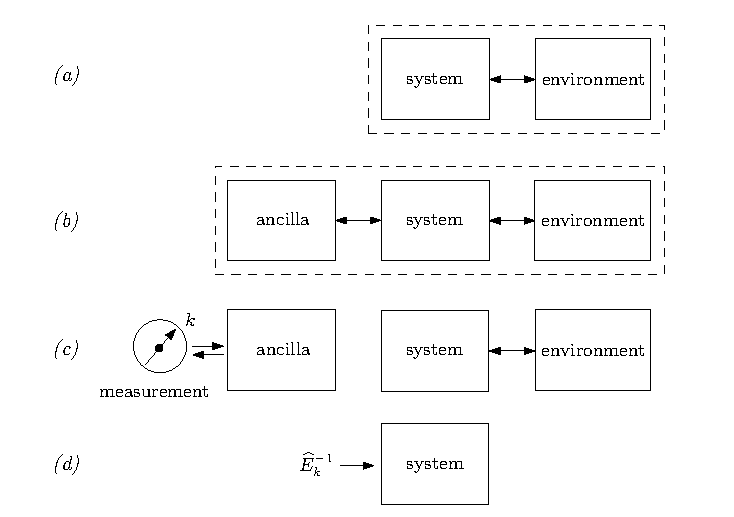
\includegraphics[width=.9\linewidth]{figures/ch07_fig02.pdf}
\caption{補助量子ビットによる量子誤り訂正。(a) 系Sと環境Eの相互作用によって、両者がもつれる［式(7.30)参照］。(b) 補助量子ビットAをSと相互作用させ、S、A、Eを含む三者もつれ状態(7.31)を作る。(c) Aへの射影測定が、この状態を式(7.33)の形の積状態へ収縮させ、実効的に部分系間のもつれを解く。測定結果には、訂正すべき誤りの情報が含まれる。(d) 適切な逆変換$\hat E_k^{-1}$の適用により、Sの元の状態が回復する。}
\end{figure}
するとアンシラの測定は、アンシラ・量子ビット・環境を合わせた全複合状態を、これらの誤りの一つに同時に収縮させ（系に、可能な誤りの集合$\{\hat E_i\}$から一つを「決める」よう「強制した」）、どの誤りが選び出されたかを教えてくれる。したがって、元の重ね合わせ状態を再構成する課題は、一つの既知の離散的誤り$\hat E_k$を反転することに帰着した。

この意味で、量子誤り訂正の基本的な考えは、Preskillの言葉を借りれば\cite{ref360}、「もつれをもってもつれに対抗する」ことである。この表現で伝えたいのは、量子ビットと環境を合わせた系を、私たちが完全に制御できる第三の「人工環境」、すなわちアンシラともつれさせれば、量子ビット系に対する環境もつれの有害な効果に対抗できる、という洞察である。誤り回復の手続きは、エントロピーを量子ビットからアンシラへ移した。したがってアンシラは、環境との相互作用によって量子ビット系に導入されたエントロピーの流しとして働く。
% 原文 p.314
\hypertarget{srcpage:314}{}\label{srcpage:314}
そのため、次の誤り訂正周期でアンシラを再利用する前に、補助量子ビットに保存された誤り情報をすべて「消去」しなければならない（すなわち、今度はアンシラを、別のエントロピーの流しへ結合しなければならない）。

上の量子誤り訂正の方式は、きわめて理想化されていた。とくに三つの問題が、実際の実現を難しくする。第一に、後の7.4.4節で論じるように、アンシラの測定によって可能な誤りすべてを区別できるような、計算用量子ビットとアンシラの相互作用を設計することは不可能である。第二に、現実的な状況では誤り演算子$\hat E_i$は非常に複雑かもしれない。対応する逆変換を、さらに大きなデコヒーレンスを加えることなく、量子コンピューターに適用できるか、どう適用するかは、なお検討を要する（その物理的実現には、計算用量子ビットと何らかの巨視的装置の相互作用が必要である）。第三に、補助量子ビットは計算用量子ビットと物理的に似ているため、計算用量子ビット自体と同じく環境との相互作用（したがってデコヒーレンス）を受けやすいと予想される。環境による補助量子ビットのこのような実効的測定は、量子誤り訂正方式の適切な動作を損なう。補助量子ビットを加えると量子コンピューター内の量子ビットの総数が増え、デコヒーレンス率は通常、系の大きさに対して指数関数的に増加するため、量子誤り訂正が実際に働くことだけでなく、意図せず量子ビットのデコヒーレンス問題をさらに悪化させないことも保証するには、精巧な実験設計が必要となる。

\subsubsectionlink{誤り訂正符号はいつ存在するか}
上の量子誤り訂正の基本原理の概説をできるだけ単純にするため、アンシラと量子ビットを合わせた系のHilbert空間に作用し、アンシラの相対状態$|a_i\rangle$がすべて区別可能で、異なる誤り型$\hat E_i$に対応するような、相関したアンシラ・量子ビット・環境状態を生むユニタリー変換が存在すると仮定した［式(7.31)参照］。すなわち、異なる二つの誤り$\hat E_i\ne\hat E_j$について$\langle a_i|a_j\rangle\approx\delta_{ij}$である。しかし、この変換が存在することをどう示し、どう決定するかという問いには、まったく立ち入らなかった。

実際、この問いは量子誤り訂正の核心にある。原理的に起こりうる、すべての誤り$\hat E_i$に対応する変換を見つけるのは、通常不可能であることがわかる。代わりに、量子誤り訂正方式が通常扱うのは、重みがある$t<N$以下であるすべての誤り$\hat E_i$を区別できる、式(7.31)の形の変換に限られる。さらに誤り訂正符号は通常、任意の初期量子ビット状態を回復できるわけではなく、量子ビット系の全Hilbert空間$\mathcal H_{\mathrm S}$の、ある部分空間$\mathcal H_{\mathrm{code}}$に含まれる状態だけを回復できる。
% 原文 p.315
\hypertarget{srcpage:315}{}\label{srcpage:315}
（部分空間$\mathcal H_{\mathrm{code}}$は、その量子誤り訂正方式の符号部分空間とよく呼ばれる。）

上の概説で見たように、量子誤り訂正の基本的方策は、誤り演算子$\hat E_i$で区別される直交部分空間へ、量子ビット状態を射影することである。そうすれば、これらの誤り部分空間のどれへ状態が射影されたかを明らかにする測定を行え、誤りを訂正するためにどの逆変換を使うかという情報を得られる。したがって形式的には、ある重み$t$までの誤りを訂正できる誤り訂正符号が存在するための十分条件（必要条件ではない）は、「誤りによって射影された」部分空間
\begin{equation}\{\hat E_i\mathcal H_{\mathrm{code}}\mid\operatorname{weight}(\hat E_i)\leq t\}\tag{7.35}\end{equation}
が、すべての$i$について（少なくとも近似的に）互いに直交することを要求することで与えられる。すると任意の初期状態$|\psi\rangle\in\mathcal H_{\mathrm{code}}$に対し、擾乱後の状態の展開に現れる異なる誤り項$\hat E_i|\psi\rangle|e_i\rangle$は互いに直交し、そのため、状態$|\psi\rangle$自体に符号化された量子情報を明らかにせずに、測定で区別できる。

\subsubsectionlink{冗長符号化の重要性と位相誤りのための三ビット符号}
条件(7.35)を満たすには、通常、冗長符号化を使う必要があることがわかる。7.4.1節では、古典計算で冗長符号化が、擾乱を受ける前の元の状態の回復にどう役立つかを説明した。また、未知の量子状態を複製できないことも述べた。しかし式(7.14)は、計算基底状態を優先基底として用い、「相対状態」の形で冗長符号化を容易に行う方法を示していることに注意しよう。すなわち、第一の量子ビットと、他のすべての量子ビットとのあいだに、CNOTゲートの列を単に適用すればよい。
\begin{equation}(\alpha|0\rangle+\beta|1\rangle)|00\cdots0\rangle\longrightarrow\alpha|000\cdots0\rangle+\beta|111\cdots1\rangle.\tag{7.36}\end{equation}
このような冗長符号化は、量子誤りの訂正にどう役立つのだろうか。

まず、こうした符号化なしには通常あまり先へ進めない理由を見るため、単一量子ビット状態$|\psi\rangle=\alpha|0\rangle+\beta|1\rangle$が環境ともつれる例を考えよう。最終的な複合状態は、次のように書ける［式(7.24)参照］。
\begin{equation}|\Psi\rangle=\frac1{\sqrt2}[(\alpha|0\rangle+\beta|1\rangle)|e_+\rangle+(\alpha|0\rangle-\beta|1\rangle)|e_-\rangle].\tag{7.37}\end{equation}
式(7.31)に含まれる仮定は、二つの直交するアンシラ状態$|a_0\rangle$と$|a_1\rangle$、およびアンシラと量子ビットを合わせた系のHilbert空間に作用するユニタリー変換が存在し、時間発展
% 原文 p.316
\hypertarget{srcpage:316}{}\label{srcpage:316}
\begin{equation}\begin{aligned}|a_{\mathrm r}\rangle|\Psi\rangle\longrightarrow\frac1{\sqrt2}\big[&|a_0\rangle(\alpha|0\rangle+\beta|1\rangle)|e_+\rangle\\+&|a_1\rangle(\alpha|0\rangle-\beta|1\rangle)|e_-\rangle\big]\end{aligned}\tag{7.38}\end{equation}
を起こせるというものである。しかし$\beta\longrightarrow-\beta$と置き換えると、「誤りの指標」としてのアンシラ状態の役割は逆転する。すなわち、今度はアンシラ状態$|a_0\rangle$が位相反転型の項と相関し、$|a_1\rangle$は誤りのない項に対応する。したがって、アンシラを測定しても、生じた誤りについて有益な情報は得られない。ただしもちろん、係数$\alpha$と$\beta$について何かを知っている場合（そして、それに応じてアンシラ状態がこれらの係数の何らかの関数である場合）は別である。しかし初期量子ビット状態は一般に完全に未知なので、このような知識があるとは明らかに仮定できない。\footnote{これはもちろん、古典的な場合にも量子的な場合にも、誤り訂正の眼目そのものである。擾乱された状態が与えられ、未知の初期状態を再構成したいのである。擾乱されていない状態が何であるべきかを最初から知っていれば、単に系をその状態へ準備し直すだけで自明に済む。}

この困難は、量子誤り訂正が、より単純な量子「消去」の方法（2.13節参照）と異なることを示す。式(7.37)と(7.38)が記述する時間発展は、本質的に「消去」手順(2.125)のものであり、アンシラと環境がそれぞれ読み出し装置と経路検出器に対応することに注意しよう。量子「消去」では、読み出し測定(2.124)の結果を、スクリーン上で観測された粒子の位置に条件付けるという意味で、干渉縞が回復される\cite{ref130}。この条件付けが必要なのは、式(2.125)の状態$|\psi_+\rangle$と$|\psi_-\rangle$が、それぞれスクリーン上の縞と「反縞」のパターンに対応し、それらを合わせたパターンは、干渉のない古典分布に等しくなるためである。したがって、干渉縞の実効的回復には、読み出し装置の最終的な相対状態$|\Phi_\pm\rangle$を区別できることが必要だが、状態$|\psi_\pm\rangle$の中の成分$|\psi_1\rangle$と$|\psi_1\rangle$の相対位相の具体的な値を、読み出し測定から推定する必要はない。これに対して量子計算では、元の重ね合わせ状態を回復することが重要である。したがって、計算基底状態間の相対位相を検出し、訂正できる必要があるが、式(7.38)はこの要求を満たさない。

この問題は、単一量子ビット状態を冗長に符号化することで解決できる。この方法を説明するため、方式(7.36)を用い、一つの論理量子ビットを三つの物理量子ビットへ冗長に符号化する例を考えよう。
\begin{equation}(\alpha|0\rangle+\beta|1\rangle)|00\rangle\longrightarrow\alpha|000\rangle+\beta|111\rangle.\tag{7.39}\end{equation}
以下で見るように、この符号化により、初期量子ビット状態をまったく知らなくても、一つの量子ビットに影響する位相反転誤りを診断し（そして回復する）ことが可能になる。

まず、符号化された状態(7.39)を、各量子ビットについて共役基底$\{|+\rangle,|-\rangle\}$へ変換する。ここで$|\pm\rangle=(|0\rangle\pm|1\rangle)/\sqrt2$である。

% 原文 p.317
\hypertarget{srcpage:317}{}\label{srcpage:317}
この変換は、いわゆるHadamard回転
\begin{equation}H=\frac1{\sqrt2}\begin{pmatrix}1&1\\1&-1\end{pmatrix}\tag{7.40}\end{equation}
を元の基底状態$|0\rangle$と$|1\rangle$に適用することで行える。基底$\{|0\rangle,|1\rangle\}$の位相反転$\hat\sigma_z$は、基底$\{|+\rangle,|-\rangle\}$ではビット反転誤りに見えることに注意しよう。なぜなら、
\begin{equation}\hat\sigma_z|\pm\rangle=|\mp\rangle\tag{7.41}\end{equation}
だからである。こうして符号化
\begin{equation}\alpha|0\rangle+\beta|1\rangle\longrightarrow\alpha|+++\rangle+\beta|---\rangle\tag{7.42}\end{equation}
を達成した。三つの量子ビットは環境と相互作用し、もつれとデコヒーレンスを受けるため、位相誤り$\hat Z_{ijk}$（$i,j,k\in\{0,1\}$）が生じる。重み1以下の誤り演算子（すなわち$\hat Z_{000}$、$\hat Z_{100}$、$\hat Z_{010}$、$\hat Z_{001}$）だけを考えるとしよう。すると、量子ビットと環境を合わせた状態は
\begin{equation}\begin{aligned}|\Psi\rangle={}&(\alpha|+++\rangle+\beta|---\rangle)|e_{000}\rangle\\&+(\alpha|-++\rangle+\beta|+--\rangle)|e_{100}\rangle\\&+(\alpha|+-+\rangle+\beta|-+-\rangle)|e_{010}\rangle\\&+(\alpha|++-\rangle+\beta|--+\rangle)|e_{001}\rangle\end{aligned}\tag{7.43}\end{equation}
と書ける。以下では、環境状態は書かないことにする。その正確な形には関心がないので、状態中の各量子ビット項が、ある環境の相対状態と相関していると考えればよい。

ここで誤りを診断したい。そのために、まず各量子ビットへHadamard回転(7.40)をもう一度適用し、元の基底$\{|0\rangle,|1\rangle\}$へ戻す。すると状態(7.43)は、（環境状態を省略して）
\begin{equation}\begin{aligned}|\Psi\rangle={}&(\alpha|000\rangle+\beta|111\rangle)\\&+(\alpha|100\rangle+\beta|011\rangle)\\&+(\alpha|010\rangle+\beta|101\rangle)\\&+(\alpha|001\rangle+\beta|110\rangle)\end{aligned}\tag{7.44}\end{equation}
となる。次に、状態$|a_{\mathrm r}\rangle=|00\rangle$に準備した二つの補助量子ビットを導入する。\footnote{実際には、これら二つの補助量子ビットは、誤りの診断と訂正の実行に厳密に必要なわけではないことを示せる。原理的には、誤り症候を、符号化された三つの量子ビット自体から直接取り出すこともできる。しかし、アンシラを含めることで、三ビット符号の説明は、上で概説した量子誤り訂正の基本的な考えを、より明瞭になぞれるようになる。さらに、いわゆる耐故障性をもつ誤り訂正方式を実現するには、補助量子ビットが必要になることがわかる（後の7.4.6節参照）。}量子ビット誤りの情報をアンシラへ符号化するため、次のようにCNOTゲート列を実行する。
% 原文 p.318
\hypertarget{srcpage:318}{}\label{srcpage:318}
\begin{enumerate}
\item まず、Sの第一および第二量子ビットから、第一の補助量子ビットへCNOTゲートを適用する。
\item 次に、Sの第一および第三量子ビットから、第二の補助量子ビットへCNOTゲートを適用する。
\end{enumerate}
三量子ビットの各計算基底状態を入力とした場合に、このCNOTゲート列がアンシラの初期状態$|00\rangle$へ及ぼす効果を、表7.2に示す。上のCNOTゲート列を適用した後、アンシラと三量子ビット系を合わせた状態(7.44)は、
\begin{equation}\begin{aligned}|\Psi\rangle|00\rangle\longrightarrow{}&(\alpha|000\rangle+\beta|111\rangle)|00\rangle\\&+(\alpha|100\rangle+\beta|011\rangle)|11\rangle\\&+(\alpha|010\rangle+\beta|101\rangle)|10\rangle\\&+(\alpha|001\rangle+\beta|110\rangle)|01\rangle\end{aligned}\tag{7.45}\end{equation}
となる。これで、四つの可能性$\hat Z_{000}$、$\hat Z_{100}$、$\hat Z_{010}$、$\hat Z_{001}$のそれぞれを、異なるアンシラ状態$|ij\rangle$（$i,j\in\{0,1\}$）と相関させたことがわかる。これらの状態は互いに直交するので、二つの補助量子ビットの測定によって、四つの誤り型を完全に区別できる。

誤り訂正手続きは、ほぼ完了した。アンシラの測定から、結果（すなわち誤り症候）「01」が得られたとしよう。この測定は、アンシラと量子ビット系を合わせた状態(7.45)を
\begin{equation}(\alpha|001\rangle+\beta|110\rangle)|01\rangle\tag{7.46}\end{equation}
へ収縮させた。アンシラはいまや量子ビット系から完全にもつれが解けたので、以下ではその状態を無視してよい。

測定結果に基づいて、誤りを訂正するために逆変換$\hat I\otimes\hat I\otimes\hat\sigma_x$を適用しなければならないことが、直ちにわかる（表7.3参照）。この変換は状態(7.46)を、次のように変える。
\begin{table}[htbp]\centering\small
\caption{左列に挙げる量子ビットと環境の各入力状態に対して、第一（中央列）および第二（右列）のCNOTゲートを適用した後の、二量子ビットアンシラの初期状態$|00\rangle$の時間発展。}
\begin{tabular}{ccc}\hline 入力&第一のCNOT&第二のCNOT\\\hline
$|000\rangle$&$|00\rangle$&$|00\rangle$\\
$|111\rangle$&$|00\rangle$&$|00\rangle$\\
$|100\rangle$&$|10\rangle$&$|11\rangle$\\
$|011\rangle$&$|10\rangle$&$|11\rangle$\\
$|010\rangle$&$|10\rangle$&$|10\rangle$\\
$|101\rangle$&$|10\rangle$&$|10\rangle$\\
$|001\rangle$&$|00\rangle$&$|01\rangle$\\
$|110\rangle$&$|00\rangle$&$|01\rangle$\\\hline\end{tabular}\end{table}
% 原文 p.319
\hypertarget{srcpage:319}{}\label{srcpage:319}
\begin{table}[htbp]\centering\small
\caption{位相反転誤りを訂正する三ビット符号。二つの補助量子ビットの測定から得られる四つの誤り症候、符号化された三量子ビット状態の対応する誤り、および元の三量子ビット状態の回復に必要な逆変換を示す。}
\begin{tabular}{cll}\hline 症候&誤り&回復変換\\\hline
00&$\hat Z_{000}$（誤りなし）&不要\\
11&$\hat Z_{100}$（第一量子ビットの位相反転）&$\hat\sigma_x\otimes\hat I\otimes\hat I$\\
10&$\hat Z_{010}$（第二量子ビットの位相反転）&$\hat I\otimes\hat\sigma_x\otimes\hat I$\\
01&$\hat Z_{001}$（第三量子ビットの位相反転）&$\hat I\otimes\hat I\otimes\hat\sigma_x$\\\hline\end{tabular}\end{table}
\begin{equation}\alpha|001\rangle+\beta|110\rangle\xrightarrow{\hat I\otimes\hat I\otimes\hat\sigma_x}\alpha|000\rangle+\beta|111\rangle.\tag{7.47}\end{equation}
したがって、最初の冗長に符号化された量子ビット状態(7.39)を回復した。最後に、符号化変換(7.39)の逆を適用すれば、擾乱を受ける前の元の単一量子ビット状態$\alpha|0\rangle+\beta|1\rangle$に到達できる。

二つ以上の量子ビットに影響する位相誤りを含めると（すなわち重み1より大きな位相誤り演算子を考えると）、この位相誤り訂正方式は、つねに成功するわけではない。これは、二つの補助量子ビットから得られる誤り情報が、二つの古典ビットにすぎないことから容易にわかる。したがって、確実に区別できる誤りの可能性は、四つまでである。三量子ビットに可能なすべての位相誤り演算子（重み0から3までのすべての演算子）を含めると、元の状態を回復できるのは、ある確率でのみとなる。今度は八つの異なる誤りを訂正できなければならないため、一つの特定の誤り症候が二つの異なる誤りに対応する。両可能性の確率を計算し、より起こりやすい誤りに対応する逆変換を適用することができる。

単一ビット誤りの確率$p$が50\%未満で、誤りが無相関であると仮定する（二量子ビット誤りと三量子ビット誤りの確率は、それぞれ$3p^2(1-p)$と$p^3$となる）。すると、最も起こりやすい誤り型は、まさに上の例で考えた$\hat Z_{000}$、$\hat Z_{100}$、$\hat Z_{010}$、$\hat Z_{001}$である。より具体的には、この方式の失敗確率は$3p^2(1-p)+p^3$（単に二量子ビット誤りと三量子ビット誤りが起こる確率）なので、失敗確率は$O(p^2)$と変化し、$p$が小さくなるとかなり急速に減少する。これは、まったく訂正しない場合の、失敗確率が$O(p)$と変化する状況と比較される（誤りが一度でも起これば状態は乱され、その確率は定義により$p$である）。したがって上の誤り訂正方式は、$p<50\%$であるかぎり、誤り訂正なしの場合より状況を改善する。この状況は、7.4.1節で論じた古典的誤り訂正の多数決方式に似ている。そこでは、平均して一つを超えるビットが反転しない場合にのみ、誤り回復が利点を与えることを示した。
% 原文 p.320
\hypertarget{srcpage:320}{}\label{srcpage:320}
すなわち、単一ビット反転の確率が50\%未満の場合である。

興味深いことに、ここで述べた位相誤りの三ビット符号は、1998年に実現された、最初の量子誤り訂正の実験的実行\cite{ref361}の基礎となった。\footnote{ただし、この実験は、上で導入した二つの補助量子ビットを用いていない。代わりに、量子ビット系に対する、ある種の共同測定から誤り症候を直接得た。}この実験は、アンサンブル量子計算装置を表すために、液体状態NMRを用いて行われた\cite{ref351}。実験で実行された量子誤り訂正手順は、理論的に予測された量子ビット系からのコヒーレンス喪失を、実際に遅らせることがわかった。

冗長符号化は、符号化しない場合より、量子コンピューター内の物理量子ビットの数を大きく増やす必要がある。そのため、大量のさらなるデコヒーレンスを導入しないよう、非常に注意深く実行しなければならない。（先に、補助量子ビットの文脈でも同様の問題を指摘した。）したがって全体を貫く目標は、物理量子ビットと論理量子ビットの比をできるだけ小さくしながら、誤り訂正能力を最大にすることである。

\subsubsectionlink{装置が引き起こすデコヒーレンスと耐故障性}
これまでは、制御されない環境との相互作用を位相誤りの源と考えてきた。しかし、この文脈の「環境」は、本来、量子ビット系と相互作用するあらゆる物理系という、より広い意味を意図している。その重要な相互作用の一つは、量子ビットを準備し、操作し、測定することで量子情報を処理する装置と、量子ビット系との結合である。装置とのこうした相互作用は、一般に装置と量子ビット系をもつれさせ、そのため量子ビットのデコヒーレンスをもたらす。たとえば、各ゲート操作は通常、ある程度の量子ビットのデコヒーレンスを生じさせる。また、実際のゲート操作はつねに不完全であり、古典的雑音を導入する。量子アルゴリズムには通常、何千ものゲートを量子ビット系へ適用する必要があり、そのため誤りが急速に蓄積する。

したがって、制御されない環境との連続的相互作用による量子ビット誤りだけでなく、量子情報の処理による誤りも周期的に訂正しなければならない。もちろん先に述べたように、誤り訂正自体も装置による測定とゲート操作に基づくため、今度はそれ自体が量子ビットにデコヒーレンス効果を導入し、どのような現実的状況でも無限の精度では実行できない。この問題は、いわゆる耐故障性をもつ誤り検出と回復の方法\cite{ref362,ref363,ref364,ref365,ref366}によって軽減できる。この方法は、個々のゲート操作と測定操作に「雑音」がある（すなわち、ある誤り確率をもつ）という現実的状況でも、量子コンピューターの信頼できる動作を保証しようとする。

% 原文 p.321
\hypertarget{srcpage:321}{}\label{srcpage:321}
耐故障性をもつ量子計算の詳細には立ち入らないが（この主題のわかりやすい総説として、たとえば文献\cite{ref056,ref367}参照）、しきい値定理とよく呼ばれる重要な結果\cite{ref360,ref368,ref369,ref370,ref371}を述べよう。耐故障性をもつ量子誤り訂正を実現すれば、ある物理的実現におけるゲート操作当たりの誤り率が、あるしきい値より小さいかぎり、\footnote{この精度のしきい値の現在の見積もりは、計算手順当たり約$10^{-2}$から$10^{-6}$まで幅がある。異なる見積もりの分析については文献\cite{ref372}参照。}少なくとも原理的には、任意の大きさの量子計算を効率よく実行できるはずだと示せる。この重要な定理は、誤りの性質について、少数の物理的に妥当な仮定を置けば証明でき、量子コンピューターの実現に基本的な障害はないはずだということを示唆する。

\subsectionlink{デコヒーレンスのない部分空間での量子計算}
デコヒーレンスのない部分空間（DFS）\cite{ref089,ref090,ref091,ref092,ref093,ref094,ref095,ref096,ref097,ref098}、またはポインター部分空間\cite{ref009}の一般的概念は、2.8.1節で導入した。DFSとは、系のHilbert空間$\mathcal H$の部分空間$\mathcal H_{\mathrm{DF}}$であり、その中の任意の状態$|\psi\rangle$が、環境との相互作用にもかかわらず、（厳密に、または近似的に）純粋なまま保たれるものであった。系を計算用量子ビットの集まりとする量子計算に適用すると、DFSにより、Hilbert空間の「静かな片隅」に量子情報を符号化して、環境の有害な影響から、その情報を自動的に保護できる。量子誤り訂正と異なり、DFSは誤りがそもそも起こることを防ぐため、本質的な誤り回避の方策を表す。

相互作用Hamiltonianの一般的な対角分解
\begin{equation}\hat H_{\mathrm{int}}=\sum_\alpha\hat S_\alpha\otimes\hat E_\alpha\tag{7.48}\end{equation}
が与えられるとき、DFSが現れるための必要条件は、演算子$\hat S_\alpha$の正規直交する縮退固有状態$|s_i\rangle$の集合が存在すること、すなわち
\begin{equation}\hat S_\alpha|s_i\rangle=\lambda^{(\alpha)}|s_i\rangle\quad\text{すべての$\alpha$と$i$について}\tag{7.49}\end{equation}
であることを示した［式(2.96)参照］。2.8.1節では、この条件が力学的対称性の存在に相当することも論じた。以下では、すべての量子ビットが、まったく同じ仕方で一つの環境と結合する模型を考える。
% 原文 p.322
\hypertarget{srcpage:322}{}\label{srcpage:322}
この場合、系と環境の相互作用は、量子ビットの任意の置換に対して完全に対称であり、最大の大きさのDFSをもたらす。独立な小さい結合項が追加されて、この完全な対称性が破れると、何が起こるだろうか。DFSには、このような摂動に対して、十分な頑健さがあってほしい。Lidar、Chuang、Whaley\cite{ref090}による初期の研究に続き、Bacon、Lidar、Whaley\cite{ref099}は、摂動の強さの一次まででは、DFS内の量子情報の保存は、このような摂動に対して、時間についてのすべての次数で安定であることを示した。しかし、DFSに符号化された量子情報の処理は、対称性を破る摂動に対して、時間の一次までしか頑健でないことがわかった。著者たちは、このDFS上の量子計算の不十分な頑健さを、DFSと能動的な量子誤り訂正方式を組み合わせることで、どのように補えるかも示した\cite{ref094}。

\subsubsectionlink{デコヒーレンスのない部分空間はどのようなものか}
これまではDFSの存在の一般条件を述べるだけで、その構造の具体例は与えなかった。また、DFSが小さすぎて、必要な高次元の重ね合わせ状態を実効的に作れないのであれば、量子計算にはほとんど役立たないことは明らかである。したがって、系の全Hilbert空間の次元に対して、DFSがどの程度の大きさをもつかという問題は非常に重要である。意外ではないだろうが、この問いに具体的に答えるには、系と環境の相互作用について特定の模型を採用しなければならない。ここでは、DFSの文献（たとえば文献\cite{ref089,ref091,ref093,ref096,ref237}参照）で最も一般的に考えられる模型、すなわち5.3節で論じたスピン・ボソン模型を考える。

\subsubsectionlink*{独立なデコヒーレンスと集団的デコヒーレンス}
量子ビットのデコヒーレンスを模型化する二つの極限を区別しよう。第一の極限は独立なデコヒーレンスであり、各量子ビットが独立に自分自身の環境と結合し、これらの環境間には相互作用がないという仮定である。この場合は7.4.2節ですでに述べた。独立なデコヒーレンスの仮定は、量子誤り訂正の文脈でしばしば置かれる。それは、量子ビットに作用する誤り過程が完全に無相関であることを意味する。したがって、ある特定の誤りが一つの量子ビットに起こる確率が$p$なら、この誤りが$K$個の量子ビットで起こる確率は$p^K$である。この場合、量子ビット誤りは、単に重み1の誤り演算子の線形結合、すなわち、他のすべての量子ビットは影響を受けない単一量子ビット誤りの組合せとして表せる。多くの誤り訂正方式（7.4.5節で論じた三量子ビット符号など）は、このような単一量子ビット誤りの訂正でのみ効率がよいため、それらの方式の基礎には、しばしば独立なデコヒーレンスの仮定がある。

しかし、量子ビットが（環境の典型的なコヒーレンス長と比べて）互いに空間的に近い場合、この仮定はあまり現実的でない。
% 原文 p.323
\hypertarget{srcpage:323}{}\label{srcpage:323}
その場合、すべての量子ビットは（近似的に）同じ環境を「感じ」、誤りは複数の量子ビット間で相関しやすい。この状況に対応する極限は集団的デコヒーレンスであり、すべての量子ビットがまったく同じ環境と結合する。

完全に独立なデコヒーレンスと、純粋に集団的なデコヒーレンスという両極端が、DFSの大きさの限界を定めることがわかる。スピン・ボソン模型では、集団的デコヒーレンスの極限で、量子ビットが多い場合、DFSの次元は元のHilbert空間の次元へ漸近的に近付き、最適な、デコヒーレンスのない符号化が可能になる。しかし反対の、独立なデコヒーレンスの極限では、論理量子ビットを符号化できるDFSが存在しないことを見る。これらの結果を確立するための詳細な模型と証明は再現しないが、それでもDFSの大きさと特定のデコヒーレンス模型の関係について、ある程度の直観を得たい。以下ではそれを行う。

\subsubsectionlink*{簡単な例}
まず、スピン・ボソン模型における集団的デコヒーレンスの場合を考えよう\cite{ref089,ref091,ref093,ref096,ref237}。ここではDFSは、ほとんど定義によって現れる。$N$量子ビットの集まりの相互作用Hamiltonianは、式(5.90)の相互作用Hamiltonianの一般化、すなわち
\begin{equation}\hat H_{\mathrm{int}}=\sum_{i=1}^N\hat\sigma_z^{(i)}\otimes\sum_j(g_{ij}\hat a_j^\dagger+g_{ij}^{*}\hat a_j)\equiv\sum_{i=1}^N\hat\sigma_z^{(i)}\otimes\hat E_i\tag{7.50}\end{equation}
で与えられる。ここで$g_{ij}$は、第$i$量子ビットと第$j$環境振動子の結合の強さを表し、$\hat a_j$（$\hat a_j^\dagger$）は、ボソン場の第$j$モードの消滅（生成）演算子である。

集団的デコヒーレンスの仮定は、すべての量子ビットが同じ環境と結合することを意味する。そのため、結合$g_{ij}$（したがって環境演算子$\hat E_i$）は添字$i$に依存してはならない。すると式(7.50)は
\begin{equation}\hat H_{\mathrm{int}}=\left(\sum_i\hat\sigma_z^{(i)}\right)\otimes\hat E\equiv\hat S_z\otimes\hat E\tag{7.51}\end{equation}
となる。環境演算子$\hat E$の正確な形は、ここではそれほど重要でない。主要な点は、相互作用Hamiltonianが式(7.51)の形に書かれ、和が一つの項$\hat S_z\otimes\hat E$に置き換わったことである。

ここで、DFSは、相互作用Hamiltonianの系演算子$\hat S_\alpha$の、縮退した固有状態の集合によって張られることを思い出そう［式(7.49)参照］。したがって、この場合のDFSは、式(7.51)で定義した集団スピン演算子$\hat S_z$の縮退固有状態によって張られる。
% 原文 p.324
\hypertarget{srcpage:324}{}\label{srcpage:324}
計算基底(7.5)で表された任意の$N$量子ビット積状態は、明らかに$\hat S_z$の固有状態である。可能な整数固有値$m$には、$m=-N$（基底状態$|1\cdots1\rangle$に対応）から$m=+N$（基底状態$|0\cdots0\rangle$に対応）まで、$2N+1$個の異なる値がある。一般に、$m_0$個の量子ビットが「0」状態にある計算基底状態の固有値は、$m=2m_0-N$である。

$\hat S_z$の同じ固有値$m$をもつ、互いに直交する計算基底状態の個数が最大になるのは、$m=0$の基底状態の集合$S_0$、すなわち「0」状態と「1」状態の量子ビットが等しい個数含まれる状態の場合である。形式的には、
\begin{equation}S_0=\left\{|i_1\cdots i_N\rangle\ \middle|\ i_j\in\{0,1\},\ \sum_{j=1}^N i_j=0\right\}\tag{7.52}\end{equation}
と書け、この集合の状態数は
\begin{equation}n_0=\binom{N}{N/2}\tag{7.53}\end{equation}
である。したがって、$S_0$に含まれる状態は、次元$n_0$のDFSを張る。$N$が大きいとき、Stirlingの公式を用い、式(7.53)の二項係数を
\begin{equation}\log_2\binom{N}{N/2}\approx N-\frac12\log_2(\pi N/2)\xrightarrow{N\gg1}N\tag{7.54}\end{equation}
と近似できる。したがって、先に述べたとおり、集団的デコヒーレンスの極限で、DFSの次元は元のHilbert空間の次元に近付き、符号化効率は1に近付く（すなわち、$N\longrightarrow\infty$の極限では、元のHilbert空間の$2^N$個すべての量子ビット基底状態を、デコヒーレンスなしに符号化できる）。

たとえば$N=4$量子ビットでは、計算基底状態の集合
\begin{equation}S_0=\{|0011\rangle,|0101\rangle,|0110\rangle,|1001\rangle,|1010\rangle,|1100\rangle\}\tag{7.55}\end{equation}
が、次元6の、最大の大きさのDFSを張る。これに対し、元のHilbert空間の次元は$2^4=16$である。したがって、ここで考えた集団的デコヒーレンス模型では、DFSの中に二つまでの論理量子ビットを符号化できる。三つの論理量子ビットには、すでに$2^3$個の計算基底状態が必要であり、式(7.55)は明らかにそれを与えない。そのため、四つの物理量子ビットを用いれば、二つ以下の論理量子ビットを必要とする、デコヒーレンスのない量子計算を実行できる。

逆に、純粋に独立なデコヒーレンスの場合には、次元が1より大きいDFSを見つけることはできない。これは次の簡単な観察からわかる。相互作用Hamiltonian(7.50)に現れる環境演算子$\hat E_i$は、今度は一般に、すべて互いに異なる。DFSを見つけるには、通常の方法(7.49)に従い、すべての$i$と$1\leq j\leq N$について
% 原文 p.325
\hypertarget{srcpage:325}{}\label{srcpage:325}
\begin{equation}\left\{\hat I^{(1)}\otimes\cdots\otimes\hat I^{(j-1)}\otimes\hat\sigma_z^{(j)}\otimes\hat I^{(j+1)}\otimes\cdots\otimes\hat I^{(N)}\right\}|s_i\rangle=\lambda^{(j)}|s_i\rangle\tag{7.56}\end{equation}
となる正規直交基底状態$\{|s_i\rangle\}$の集合を求める。読者が容易に確認できるように、この固有値問題を満たす状態は、計算基底状態$|0\cdots0\rangle$という、ただ一つの状態だけである。一つの論理量子ビットを符号化するにも、少なくとも二次元の部分空間が必要なので、スピン・ボソン模型の独立なデコヒーレンスの場合には、量子計算のためのDFSは存在しえない。ポインター部分空間の言葉では、厳密なポインター状態は一つしかなく、系の、この環境によって超選択された優先状態は、基底状態$|0\cdots0\rangle$となる。

もちろん、現実的な状況では、純粋に独立なデコヒーレンスという仮定も、完全に集団的なデコヒーレンスという極限も、完全には適切でない。しかし幸い、この二つの極限それぞれでデコヒーレンスに対抗する、強力な相補的方法がいまや二つある。DFSへの符号化によって、量子ビット系を集団的デコヒーレンス効果から保護し、7.4節で述べた能動的な誤り訂正法によって、独立なデコヒーレンスに起因する単一量子ビット誤りから回復できる。実際、両方法は結び付ける（または「連接する」\cite{ref094}）ことができ、それによって単一量子ビット誤りへの制限を外しても、耐故障性をもつ普遍量子計算が可能になる\cite{ref095,ref373}。

\subsubsectionlink{デコヒーレンスのない部分空間の実験的実現}
DFSの存在を明示的に実証した最初の実験の結果は、Kwiatと共同研究者が2000年に報告した\cite{ref374}。この実験は、量子計算に関係するDFSを実際に実現したというより、原理の実証であったことを強調すべきである。単に、一対の光子のある特定のBell状態［式(2.7)参照］が、集団的デコヒーレンスに対して本質的に免疫をもつ一方、他の三つのBell状態の光子対は、理論予測と一致して、大きなデコヒーレンスを受けることが示された。この実験では、人工環境として、二つの光子の経路に対して調整可能な角度に向けた、小さな二片の石英を用い、その中を通過する光子に、制御できるデコヒーレンス相互作用を生じさせた。二片の石英を同じ角度（$90^\circ$を法として）にそろえると、集団的デコヒーレンスが生じた。角度を変えることは、異なる基底でデコヒーレンスを生じさせることに対応した。本質的には、この実験は単一のポインター状態の存在を示しただけである。

DFSに関する別の実験の結果は、NISTのKielpinskiらが2001年に報告した\cite{ref375}。彼らは、前の段落で述べたKwiatらの実験\cite{ref374}と同様の、二量子ビットBell状態を用いた。しかし今回は、捕獲され、強く相互作用する一対の$^9\mathrm{Be}^+$イオンのDFSへ、一つの論理量子ビットを符号化した。この実験は、符号化された基底状態の重ね合わせが、実際に集団的デコヒーレンスの影響を受けないことを示した。観測されたコヒーレンスの減衰は、符号化されていない量子ビット状態に比べてはるかに遅かった。
% 原文 p.326
\hypertarget{srcpage:326}{}\label{srcpage:326}
その減衰は、集団的デコヒーレンス以外の原因（読み出しパルスの劣化や、イオンの運動状態の加熱など）に帰属できた。したがってこの実験は、物理量子ビットの四次元Hilbert空間を用いて、集団的デコヒーレンスの影響を受けない二次元部分空間を実験的に構築することに成功した。

それ以来、実験は、量子ビットの異なる物理的実現を用い、ますます大きなDFSを作ろうとしてきた。たとえばViolaらは2001年に、NMR量子ビットを用い、初めて三量子ビットDFSの生成に成功した\cite{ref376}。

\subsubsectionlink{環境工学と動的分離}
実用上、すなわち実験的に関心のある状況で、少なくとも近似的にでも、DFSの存在条件をどこまで満たせるかと疑問に思うかもしれない。前節では、実際にDFSを実現した近年の実験をいくつか説明した。しかし、そのDFSはまだ非常に小さい。相当に大きなDFSが存在するには、系と環境の相互作用が、十分に高い対称性を示さなければならないことは明らかであり、与えられた実験状況で、こうした条件が自然に生じる可能性は低いように思われる。

この制限を克服する可能な方法の一つは、環境工学に基づく。ここでは、系と環境の相互作用の構造に、ある種の対称性を能動的に作り出そうとする。明らかな理由から、この方策はときに「環境の対称化」とも呼ばれる。たとえばDalvit、Dziarmaga、Zurek\cite{ref102}は、系と環境の結合を適切に設計して対称化すれば、Bose--Einstein凝縮体の重ね合わせ状態を、相互作用Hamiltonianの（近似的に）縮退した固有状態に対応させられることを示した。したがって、こうした重ね合わせ状態はDFS内に属し、その寿命を大きく延ばすことになる（6.4.1節も参照）。

Poyatos、Cirac、Zoller\cite{ref377}が示したように、捕獲イオンの実効的な系・環境相互作用Hamiltonianのパラメーターを変えることで（制御するレーザー光が環境の役割を果たす）、異なるポインター部分空間を選び、系（捕獲イオン）がどのDFSへ駆動されるかを能動的に制御することもできる。この特徴はその後、デコヒーレンスの制御と模擬への応用として、イオントラップ実験で実証された\cite{ref125,ref353}（文献\cite{ref378}も参照）。これは、ポインター基底という概念に直接の実験的証拠を見事に与える。「古典的」状態の形は、量子力学の外から持ち込まれた、何らかの先験的基準であらかじめ定められているのではなく、2.8節で述べたように、系と環境の相互作用Hamiltonianの構造によって動的に定まる。この相互作用Hamiltonianを変えると、異なる準古典的状態に対応する、さまざまなポインター基底が現れる。

DFSを能動的に作り出す別の方法は、動的分離として知られるようになった\cite{ref379,ref380,ref381,ref382,ref383,ref384}。ここで基本的な工夫は、環境の影響を実効的に打ち消すよう、系のHamiltonianへ時間依存の変更を加えることである。
% 原文 p.327
\hypertarget{srcpage:327}{}\label{srcpage:327}
これらの変更は、系だけに作用する、高速な射影測定列や強い制御場パルス列の形を取る（「量子バンバン制御」\cite{ref379}）。系と環境の相互作用Hamiltonianの構造をまったく知らなくても、分離用の制御場の速度を無限に速くする極限では、デコヒーレンスを任意によく抑制でき、その結果DFSを動的に作り出せる（この場合、それは動的に分離された部分空間を表す）。制御速度が有限である現実的な場合にも、制御速度が、環境もつれの形成率によって定まる最も速い時間尺度を上回れば、この分離技法によって、十分な（完全ではないが）デコヒーレンスからの保護を達成できる。

\subsectionlink{まとめと展望}
量子コンピューターの実現にとって主要な障害は、必要とされる遮蔽と制御可能性のトレードオフである。一方では、デコヒーレンスを最小化するため、望ましくない環境との相互作用から十分に保護された量子ビット系を構築する必要がある。他方では、量子計算の実行に必要なコヒーレント制御を可能にするため、これらの系は十分に開かれたままでなければならない。

このように量子ビットを単に孤立させられない以上、量子計算でデコヒーレンスを最小化するには、能動的な量子誤り訂正、デコヒーレンスのない部分空間、環境工学、動的分離などの技法を、つねに組み合わせる必要がある。単一量子ビット誤りだけに限るという（通常、あまり現実的でない）制限を外すと、耐故障性をもつ普遍量子計算を達成するには、DFSと量子誤り訂正の両方を用いる必要があることを示せる\cite{ref373}。そこでの考えは、まず、動的な対称性を利用する（あるいは作り出す）ことで、十分な程度に近似的なデコヒーレンスのない部分空間へ符号化できるように、量子コンピューターを構築することである。量子ビット系の時間発展に外部から時間依存の変更を加えることで、量子計算の途中にも、実効的なDFSを作り、維持できる。DFSは理想条件からの小さい摂動にある程度頑健なので、この方法は、量子計算にデコヒーレンス効果に対する、ある程度の安定性をもたらす。その後、第二の段階として、量子誤り訂正方式を用い、デコヒーレンスの影響から能動的に回復しようとすることができる。

現在までにコヒーレントに制御できているのは、ほんの一握りの量子ビットであり、有用な量子計算を行うには、まったく足りない。デコヒーレンス時間を十分に延ばし、動作する量子コンピューターの構築を可能にできるか、またそれがいつになるかは、なお今後を待たなければならない。いずれにせよ、量子計算への関心に促された、デコヒーレンスに対抗する方策の研究は、デコヒーレンス自体の理論的・実験的理解を深めるうえでも、実り豊かであった。
% 原文 p.328
\hypertarget{srcpage:328}{}\label{srcpage:328}
デコヒーレンス研究の初期には、量子測定と、一般的な量子から古典への移行に対する基礎的含意に焦点が当てられ、関心の中心は、デコヒーレンスの実際上不可逆な性質と、その極端な効率のよさであった。過去10年のあいだに、量子計算の分野は、デコヒーレンスを生む相互作用の能動的な制御と設計に焦点を当てることで、この範囲を大きく広げた。たとえば、系と環境の相互作用の構造を設計・操作し、デコヒーレンスの影響の小さいHilbert空間の隙間を利用し、作り出す方法を学び、実験的に実証してきた。量子誤り訂正は、デコヒーレンス効果の影響と軽減を、離散的な誤りという言葉で表すようにした。これらの誤りは、デコヒーレンスを引き起こすまさにその効果、すなわち量子もつれを利用することで、実効的に「取り消す」ことができる。さらに多くの例をここに挙げることができ、そのいくつかは本章で論じた。この意味で、デコヒーレンスについての理解は、近年の量子計算の研究から大きな刺激を受けてきた。この研究分野から、デコヒーレンスについての、さらに多くの刺激的な洞察が得られることを期待できる。

\clearpage
\setcounter{section}{7}
\setcounter{footnote}{0}

% 原文 p.329
\hypertarget{srcpage:329}{}\label{srcpage:329}
\sectionlink{量子力学の解釈におけるデコヒーレンスの役割}
\setcounter{footnote}{0}

物理学者の精鋭たちが量子力学の解釈について激しい議論を交わした、1927年の有名なSolvay会議\cite{ref385}から、すでに何十年もの歳月が過ぎた。それでも、量子論の意味をめぐる議論には衰える兆しがない。量子力学に対する純粋に実用主義的な「黙って計算せよ」という姿勢\footnote{この呼称はしばしばFeynmanに帰されるが、「黙って計算せよ解釈」というあだ名を実際に作ったのはMermin\cite{ref386}らしい。このような解釈上の立場の例として\cite{ref044}を参照されたい。}を超え、量子形式と、私たちの「外部」にあると想定される物理的実在とを結びつけようとすれば、解釈の問題に巻き込まれることはほとんど避けられない。したがって、多様な量子力学の解釈の存在は、量子論そのものと同じくらい古い。

本章では、次の重要な問いを論じる。デコヒーレンス自体が量子力学の解釈上の問題と関係していることを踏まえると、デコヒーレンスはこれらの異なる解釈にどのような含意を持つのだろうか。この問いは、とりわけ興味深い。というのも、相対状態解釈、様相解釈、de BroglieとBohmのパイロット波理論など、主要な解釈の多くがすでに定式化されてから、かなり後になってデコヒーレンスが「発見」されたからである。（第1章の末尾で述べたように、デコヒーレンスが科学者の共同体から広く注目され始めたのは、1990年代の初めになってからにすぎない。）量子測定のような解釈に関係する主題を現実的に記述するうえで、デコヒーレンスが重要であるとようやく認識されると、既存の、また将来の量子力学の解釈に対するその含意を問うことが、切実な意味を持つようになった。解釈の主要な目的の一つは量子測定の不可解な側面を理解することであり、デコヒーレンスは、とりわけそのような測定の現実的な記述を扱っていた。したがって、デコヒーレンスから得られた新しい知見を踏まえて、これらの解釈を再検討することは避けられなかった。

量子力学の解釈に対するデコヒーレンスの含意を調べる際に出会う、いくつかの重要な問いを挙げよう。

% 原文 p.330
\hypertarget{srcpage:330}{}\label{srcpage:330}
\begin{itemize}
\item デコヒーレンスだけで量子力学の基礎に関する特定の問題を解決し、個々の解釈が量子力学に導入した解釈上ないし形式上の付加物の一部を不要にできるだろうか。もしできるなら、どのような核心的な基礎問題が残り、それらはどのような形を取るのだろうか。
\item デコヒーレンスは解釈の経験的適合性を保証できるだろうか。すなわち、ある解釈が実験によって反証されるのを防ぐことができるだろうか。
\item 逆に、デコヒーレンスは、ある解釈が標準量子力学や観測と衝突することを示すことによって、その解釈を排除できるだろうか。
\item デコヒーレンスは、個々の解釈が導入する仮定の一部に物理的な動機を与え、それによって、それらの仮定にいっそう明確な物理的意味を与えることができるだろうか。
\item デコヒーレンスは、さまざまな解釈を統合し簡素化する「融合剤」として、どの程度まで働くことができるだろうか。そうすることで、一見異なる解釈を共通の核心へ還元できることを示せるだろうか。
\end{itemize}
本章では、これらの問いやほかの問いを、量子力学の主要な解釈の流れごとに取り上げ、分析する。本章の一部は、著者の総説\cite{ref001}\footnote{本章の一部は、許可を得て\cite{ref001}を改作したものである。Copyright 2004 by the American Physical Society.}に基づいている。標準解釈とCopenhagen解釈（8.1節）、相対状態解釈（8.2節）、様相解釈（8.3節）、物理的収縮理論（8.4節）、Bohm力学（8.5節）を考察する。これによって、デコヒーレンスに照らして異なる解釈の現状を評価できるだけでなく、デコヒーレンス自体の意味と適用範囲についても、新しい知見が得られるだろう。

\subsectionlink{標準解釈とCopenhagen解釈}
本節では、量子力学の教科書の大部分で、明示的または暗黙的に示されている標準解釈を論じる。この解釈は、量子力学の「正統的」解釈とも呼ばれることが多い。ここでは、標準解釈とCopenhagen解釈\footnote{実際には、単一で首尾一貫した「Copenhagen解釈」は存在せず、Bohr、Heisenbergおよび同時代の人々による、時には食い違う見解の寄せ集めであることが指摘されており\cite{ref387}、現在では広く認識されている。ここでの議論は、BohrとHeisenbergが提起した解釈上の考え方を指すものとする。ただし、両者の考え方を区別する必要がある場合も多い。}を意識的に区別する。後者は、測定を含む量子現象を記述するために、基本的で還元不可能な古典的概念が必要であるという追加の仮定を導入するからである。
% 原文 p.331
\hypertarget{srcpage:331}{}\label{srcpage:331}
Copenhagen解釈のこの特徴には、後の8.1.3節で立ち戻る。Copenhagen解釈とデコヒーレンスの関係に関する詳しい議論は\cite{ref388}にある。\cite{ref389,ref390}も参照されたい。

標準解釈を特徴づけるのは、本書のさまざまな箇所ですでに触れた収縮公準である。この公準はいくつかの部分に分けられる。第一に、量子系に対して行われるすべての測定は、ユニタリーな時間発展に不連続な中断を生じさせる。第二に、この中断によって、測定される観測量の固有状態で展開された波動関数が、それらの項の一つへ「収縮」する。こうして、重ね合わせの一成分が測定結果として選ばれる。第三に、ある特定の結果の確率は、初期波動関数と、その結果に対応する量子状態との重なりの振幅の絶対値の二乗で与えられる（Born則。原著35頁の脚注9も参照）。

標準解釈は、収縮の本性について何の説明も与えない\footnote{他方、Copenhagen解釈は、収縮の認識論的性格を強調しているように見える。この解釈では波動関数を確率振幅だけを表すものとみなすため、収縮は実際の物理過程というよりも、単なる「情報の増加」という性格を持つ。2.1節の議論も参照されたい。}。この解釈における測定と収縮公準の際立った役割にもかかわらず、「測定」の具体的な定義はかなり不明確なままである。原理的には、標準解釈は「古典的」状態の巨視的重ね合わせの可能性を、あらかじめ排除しない。同時に、そのような重ね合わせを観測する行為は、収縮を引き起こす測定相互作用にほかならないから、決して観測できないともいう。しかし、厳密に何が測定に当たるのかという問いには、答えが与えられない。収縮を引き起こすには人間の観測者が必要なのだろうか。ある相互作用はいつ収縮を引き起こし、いつ系がユニタリーに発展し続けることを許すのだろうか。

\subsubsectionlink{結果の問題}
結果の問題は、von Neumannの測定図式との関連ですでに論じた（2.5.4節参照）。そこで述べたように、標準解釈では、結果、すなわち確定した「値」の存在に関する解釈規則は、固有値・固有状態リンクによって与えられる。この規則は、系がある物理量について確定した値を持つのは、その物理量に対応する観測量の固有状態にある場合、かつその場合に限ると定める。これは「客観的な」基準である。なぜなら、ある物理量の値を帰属させられる、系の確定した量子状態の存在を推論できるからである。

この解釈の枠組みの中では、収縮公準を前提としない限り、デコヒーレンスは2.5.4節で述べた結果の問題を解決できない。
% 原文 p.332
\hypertarget{srcpage:332}{}\label{srcpage:332}
巨視的に異なる指針状態間の位相コヒーレンスは、環境を含む状態では保存されており、系を拡大して環境の少なくとも一部を含めることが、いつでもできるからである。言い換えれば、コヒーレンスが環境へ非局在化することによって、重ね合わせが拡大されるだけであり（「干渉項は依然として存在するが、そこにはない」\cite[224頁]{ref007}）、デコヒーレンス過程は原理的には常に逆転できる。したがって、物理量の確定した値の存在を正統的な固有値・固有状態リンクで確立すると仮定するなら、デコヒーレンスは、系が実際にいつか一つの確定した指針状態にあることも、そもそも測定に結果があることも保証できない。もちろん、系が初めから指針観測量の固有状態にある場合は別である。

この重要な点を、もう少し詳しく論じよう。まず、全体の系・環境量子状態ベクトルについていえば、環境との相互作用はもつれを追加しただけであることに注意しよう。
\begin{equation}
|\Psi(t=0)\rangle=\Bigl(\sum_n c_n|s_n\rangle\Bigr)|E_0\rangle
\longrightarrow |\Psi(t)\rangle=\sum_n c_n|s_n\rangle|E_n(t)\rangle .\tag{8.1}
\end{equation}
ある意味では、環境との相互作用が生み出すもつれは、von Neumann図式で考えられる測定問題（2.5節参照）を、最初はかえって悪化させるとさえ考えられる。Bacciagaluppi\cite[3.2節]{ref391}は、この点を次のように述べている。
\begin{quote}
直観的には、環境が私たちの介入なしに多数の近似的な位置測定を行っているなら、測定問題は、そのように自発的に起こる測定にも、より広く当てはまるはずである。（中略）物体と環境の状態は、非常によく局在した無数の項の重ね合わせとなり得る。それぞれの項はわずかに異なる位置にあり、それら全体は、日常的な物体の場合でさえ、巨視的な距離にわたって広がっている。（中略）あらゆるものがほかのあらゆるものと相互作用しているなら、あらゆるものがほかのあらゆるものともつれていることになり、それは測定装置と測定対象のもつれよりも悪い問題である。
\end{quote}
環境の相対状態の重なり$\langle E_n(t)|E_{m\ne n}(t)\rangle$が急速に減少すること、すなわちそれらの状態の識別可能性が増すことが意味を持つのは、量子力学の通常の測定公理に基づいて局所測定を考えるようになってからである。たとえば、状態(8.1)に対応する系の縮約密度行列を作ると、
\begin{equation}
\hat\rho_{\mathrm S}(t)=\sum_{mn}c_m c_n^*|s_m\rangle\langle s_n|\langle E_n(t)|E_m(t)\rangle .\tag{8.2}
\end{equation}
2.7節で論じたように、重なり$\langle E_n(t)|E_{m\ne n}(t)\rangle$の急速な減衰は、干渉項$|s_m\rangle\langle s_{n\ne m}|$が抑制されることを意味する。
% 原文 p.333
\hypertarget{srcpage:333}{}\label{srcpage:333}
縮約密度行列は、成分状態$|s_n\rangle$の、近似的ではあるが非真正の集団へ変わる。
\begin{equation}
\hat\rho_{\mathrm S}(t)\approx\sum_n|c_n|^2|s_n\rangle\langle s_n| .\tag{8.3}
\end{equation}
縮約密度行列を導入した動機は、この数学的対象が局所系のすべての測定統計を完全に含んでいるという事実であったことを思い出そう。これらの統計は、可能なすべての局所観測量$\hat O_{\mathrm S}$の期待値によって与えられ、トレース規則$\langle\hat O_{\mathrm S}\rangle=\operatorname{Tr}(\hat\rho_{\mathrm S}\hat O_{\mathrm S})$から計算される。実用上あらゆる目的について、また系だけに対するいかなる局所測定についても、系の縮約密度行列(8.3)が生成する統計は、それに対応する純粋状態の真正混合、すなわち集団が生成する統計と、近似的に同じになる。この純粋に操作的な意味で、デコヒーレンスは、特に巨視的領域において、ある種の干渉効果がなぜこれほど観測しにくいのかを説明する（2.7節と2.5.3節も参照）。

しかし、トレース操作は非ユニタリーであり、一般には測定の異なる結果についての平均という動機と解釈を与えられていることに注意しよう。2.4.1節で示したように、形式的な式$\operatorname{Tr}(\hat\rho\hat O)$を、演算子$\hat O$が表す量の期待値と同定する根拠は、次の数学的事実にある。このトレースを書き下すと、$\hat O$が表す測定の可能な結果について、それぞれの結果に対応する特定の状態へ測定中に系が「投げ込まれる」Born確率で重みをつけた和と等しくなるのである。しかしこの解釈は、測定に結果があり、Born則が成り立つことを、すでに前提としている。したがって、トレース操作、そして縮約密度行列の概念とその解釈は、統計的解釈と、量子力学の通常の測定公理に基づいている。Pessoa Jr.\cite[432頁]{ref064}の言葉では、「部分トレースを取ることは、射影公準の統計的な形に相当する」。

量子力学の標準解釈において、結果の存在を保証し、それゆえ系へ物理量の確定した値をいつ割り当てられるかを定めるのは、まさにこの射影公準、すなわち収縮公準である。したがって、縮約密度行列のように、トレース規則によって得られる形式的構造から、その結果の存在を導くことはできない。測定公理、したがってトレース規則を取り去ると、残るのは全体の系と環境がもつれた状態(8.1)である。標準解釈によれば、この状態からは系の物理状態について何もいえず、特定の結果、すなわち物理量の確定した値を、系へ割り当てることもできない。


% 原文 p.334
\hypertarget{srcpage:334}{}\label{srcpage:334}
\subsubsectionlink{観測量、測定、環境誘起超選択}
標準解釈とCopenhagen解釈では、物理的性質の割り当ては、ある物理量の測定を表す観測量によって定められ、その観測量が優先基底を定義する。しかし、任意のHermite演算子が観測量の役割を果たせるから、どのような状態も、無限個の異なる性質を潜在的に持っている。それらの性質の帰属は通常、相互排他的である。ただし、対応する観測量が可換な場合は別であり、その場合は共通の固有基底があるため、優先基底の一意性が保たれる。それでは、測定される観測量を何が決めるのだろうか。標準解釈とCopenhagen解釈では、本質的には「利用者」が、測定する特定の観測量を単に「選び」、それによって系がどの性質を持つかを決めるのである。

この実証主義的な見方は、多くの論争を生んできた。それは、自然科学が始まって以来その核心をなしてきた、観測者に依存しない実在という考えに反する。さらに、実際には、任意の観測量を自由に選んで測定できるわけではない。私たちが持つのは、特定の観測量を測定するように作られた、感覚器官をも含む「装置」である。ほとんどの、そしておそらくすべての実用的目的について、これは最終的には一つの関係する観測量、すなわち位置に帰着するだろう。しかし、装置を特定の観測量に適したものにしているのは何だろうか。

この決定的な問いに答えるには、実際の物理的測定の仕組みと、仮にあってもわずかな関係しか持たない「ブラックボックス」過程として測定を扱う、正統的な見方を本質的に捨てなければならない。測定を、系と装置の間に量子相関が形成されることとして形式化する考えは、量子力学の初期にさかのぼり、von Neumannの測定図式にも表れている（2.5.1節参照）。しかし、2.5.2節で論じたように、それだけでは、観測量がどのように選ばれるかという問題は解決しない。第二の要素、すなわち測定過程の記述に環境を明示的に含めることは、デコヒーレンスの研究によって量子論へ持ち込まれた。Zurek\cite{ref008}が導入した指針状態の安定性基準は、測定が頑健な記録を確立するような性質を持たなければならないことを意味する。すなわち、周囲の環境との避けられない相互作用にもかかわらず、系と装置の相関が保存されなければならないのである（2.8節の議論参照）。「利用者」は観測量を任意に選ぶことはできず、環境との相互作用が安定した記録を保証するような測定装置を設計しなければならない。それによって、その観測量に対する測定装置が定義される。正統的量子力学の読み方では、これは環境が系の性質を決定していると解釈できる。

この意味で、デコヒーレンスの研究計画は、標準解釈とCopenhagen解釈が提起する、観測者が自由に選ぶように見える観測量という曖昧な概念を伴った、かなり形式的な測定概念を、より現実的で物理的な動機を持つ枠組みへ組み込んだ\cite{ref388}。
% 原文 p.335
\hypertarget{srcpage:335}{}\label{srcpage:335}
これは、測定装置の物理的構造と環境との相互作用を考慮し、測定される観測量を選ぶための、観測者を必要としない基準を指定することによって実現される。ほとんどの場合、測定記録を増幅し\cite{ref076}、それによって外部観測者が利用できるようにするためにも、環境が必要である（2.9節も参照）。

\subsubsectionlink{Copenhagen解釈における古典性の概念}
Copenhagen解釈は、さらに、古典性は量子力学から導かれるべきものではないとする。たとえば、基礎にある量子構造の巨視的極限として導くべきものではない。標準解釈では、ある意味でそう仮定しているが、明示的には導いていない。代わりにCopenhagen解釈は、古典性を完全な量子論の不可欠で還元不可能な要素、さらには量子論に先立つ概念とみなすべきだと定める。特に、古典物理学に従い、量子力学的には記述すべきでない巨視的測定装置の存在を仮定する。この点はvon Neumannの測定図式と著しく対照的である。そのような古典的装置は、私たちの経験する「古典的」世界の言葉で量子力学的現象に接近するために必要だと考えられる（たとえば\cite[209頁]{ref072}参照）。量子力学で記述すべき系と、古典物理学に従う装置とのこの二元論は、系と装置の間に、原理的には移動可能であるとはいえ、基本的な境界が存在することも意味する。その境界は微視的世界を巨視的世界から分ける（「Heisenberg切断」\cite[15頁]{ref392}）\footnote{\cite{ref388}で詳しく論じられているように、BohrとHeisenbergは、切断についてかなり異なる考えを持っていたようである。特にHeisenbergは、切断の位置は「物理的に確定することができない」、それは物理的不連続を表すものではない\cite[49頁]{ref393}とし、「しかも、切断の位置を選ぶ際の恣意性こそが、量子力学の適用にとって決定的なのである」\cite[416頁]{ref394}と述べた。これに対し、Heisenberg\cite[24頁]{ref395}が回想するところでは、「Bohrは、対象と残りの世界との分割は任意ではないと述べる方が、より現実的であることを強調していた」のであり、対象は実験自体の本性によって定まる。Howard\cite{ref396}も、Bohrにとって量子・古典の区別は、対象・装置の区別と厳密に一致してはいなかったのに対し、Heisenbergにとっては、まさに一致していたように見えると論じている。}。

Bohr、Heisenbergたちが「還元不可能な古典的概念」の必要性を主張したとき、厳密に何を意味したのかを理解することは、難しいことで知られる。詳しい議論については、たとえば\cite{ref388,ref396}を参照されたい。デコヒーレンスによる古典性の創発という研究計画に照らして、そのような古典的概念の基本的な考え方が不要になるのか、あるいは維持不能にさえなるのかは、それらの概念に認識論的、物理的といったどのような地位を与えるかに、大きく依存する\cite{ref388}。
% 原文 p.336
\hypertarget{srcpage:336}{}\label{srcpage:336}
明らかなのは、環境誘起超選択と干渉の抑制が、量子形式だけを用い、微視的尺度から巨視的尺度までの広い範囲にわたり、準古典的で頑健な状態がどのように出現し、あるいは出現しないままでいるかを示してきたことである。これは、系と装置との境界を、かなりの程度まで装置の側へ動かせることを示す近年の実験（第6章参照）と、非常によく一致している。同様の結果は、環境による系の監視を含む、量子非破壊測定の一般的研究からも得られている（たとえば\cite{ref138}の第19章参照）。このように、デコヒーレンスはHeisenberg切断の位置を一義的に指定し、量子・古典の区分と、その境界における動力学に、物理的で定量的な基盤を与える。

Copenhagenの見方では、装置は古典的に記述されるので、定義上巨視的だということに注意しよう。しかし、実際の「計器」は、微視的であってもよい。巨視的でなければならないのは、測定記録の実効的な不可逆性と冗長性を保証する「増幅器」だけである。この点を最初に強調したのはZurek\cite{ref076}である。\cite{ref016,ref323,ref389}における彼の議論も参照されたい。例として、2.10節で述べたデコヒーレンス模型を考えよう。ここでは、系は二安定原子で表された「計器」に対応し、環境が増幅器の役割を果たす（「ビットをバイトで測定する」）。同様に、ある種の巨視的測定装置も、「微視的な」量子力学的言葉で記述できる。例として、重力波の巨視的検出器\cite{ref069}や、量子限界における位置測定\cite{ref310}を実現するための、量子電気機械系\cite{ref307}における巨視的共振器がある（6.4.2節参照）。どちらの装置も、量子力学的調和振動子として扱うことができる。

デコヒーレンスの研究計画がすでに達成した進歩に基づけば、何らかの追加的な解釈構造に組み込まれたデコヒーレンスによって、量子力学的原理から古典世界の現れを、完全かつ整合的に導けるようになると予想するのは合理的である。物理的な観点からは、量子力学の領域外で扱わなければならない、本質的に古典的な装置を仮定することは、必要でも実行可能でもないように見えるだろう。このようにして、古典世界の必要性というBohrの認識論的考えの正しさを認めると同時に、古典世界を、純粋に量子力学的な基盤の一部であり、そこから出現するものとみなすことができる\cite{ref067,ref104,ref388,ref391}。

\subsectionlink{相対状態解釈}
正統的量子力学の系・観測者二元論は、量子系の決定論的法則で記述されず、代わりに確率的な非決定性に従う、外部の「観測者」を理論へ導入する。この方法は、宇宙全体を考えると、明らかに問題に突き当たる。定義上、外部の観測者は存在できないからである。


% 原文 p.337
\hypertarget{srcpage:337}{}\label{srcpage:337}
相対状態解釈の中心的考えは、この系・観測者二元論を捨てることである。この考えは1950年代末にHugh Everett\cite{ref140}が初めて述べ、ただし詳細には展開せず、その後多くの著者が発展させた。代わりに、(i)宇宙全体の物理状態を表す全量子状態$|\Psi\rangle$の存在を仮定し、(ii)Schrödinger発展の普遍的妥当性を維持する。さらに、(iii)測定終了時に、全状態を測定観測量の固有基底で展開したすべての項が、ある意味で物理状態に対応すると仮定する。すなわち、形式上も物理上も、特定の「結果」は選ばれない。これらの各物理状態は、(a)複合系の他方の部分の状態に対して相対的なもの（Everettの原案。\cite{ref141,ref143}も参照）、(b)絶えず「分裂」する宇宙のある「分枝」に対して相対的なもの（DeWitt\cite{ref397}とDeutsch\cite{ref398}が広めた多世界解釈）、あるいは(c)意識的観測者の心の集合における、特定の「心」に対して相対的なもの（多心解釈。たとえば\cite{ref399}参照）と理解できる。

相対状態解釈は、二つの大きな困難に直面する。第一は優先基底問題である。状態が相対的なものにすぎないなら、何に対して相対的なのかという問いが生じる。分枝を定義するために使われ、次の瞬間に相対的な性質、世界、心を指定する、特定の基底項を何が決めるのだろうか。「分裂」は厳密にいつ起きるのか。それぞれの分枝でどの性質が確定し、それらは私たちが経験する確定した性質とどのようにつながるのか。第二に、可能なすべての結果がある意味で「起こる」なら、確率は何を意味し、そのような解釈の枠組みでBorn則をどのように動機づけられるのか。以下で述べるように、相対状態解釈の支持者は、これらの困難を解決するため、しばしばデコヒーレンスに訴えてきた（たとえば\cite{ref398,ref400,ref401,ref402,ref403,ref404,ref405,ref406,ref407}参照）。

他方、ZehやZurekのようなデコヒーレンス研究の先駆者も、Everettの相対状態の枠組みの考え方を、しばしば利用してきた（たとえば\cite{ref004,ref005,ref104,ref408}参照）。これはおそらく、Everettの方法が、解釈上の追加要素を最小限にして、ユニタリー量子力学を本質的に「そのまま」受け入れるためだろう。この姿勢は、基本的な量子力学の形式だけから古典性の出現を説明しようとする、デコヒーレンス研究の精神によく合う。Zehは、異なる観測者が付随するEverett型の分枝を支持している\cite{ref408}（9.4節も参照）。Zurekは、優先基底問題を明確に示し\cite{ref008}、安定な測定記録の重要性と役割を強調する\cite{ref084,ref104}ために、相対状態を有用な概念として用いた（後の8.2.3節で述べるZurekの「実存的解釈」参照）。

\subsubsectionlink{Everett分枝と優先基底問題}
Stapp\cite[1043頁]{ref409}は、「量子論の多世界解釈が存在するのは、付随する基底問題が解決される限りにおいてのみである」という要件を述べた。
% 原文 p.338
\hypertarget{srcpage:338}{}\label{srcpage:338}
相対状態解釈では、優先基底問題は正統的解釈におけるよりもはるかに深刻であるだけでなく、少なくとも次の二つの理由によって、より根本的でもある。
\begin{enumerate}
\item 分枝は連続的に、しかも本質的にあらゆる場所で起こる。測定を量子相関の形成という一般的な意味で理解するなら、新たに形成される相関は、微視的な系に関するものであれ巨視的な系に関するものであれ、すべて分枝に対応する。
\item 少なくとも世界や心の実際の「分裂」を仮定する相対状態解釈では、存在論的含意ははるかに劇的である。基底の選び方が、結果として生じる「世界」や「心」全体を決めるからである。
\end{enumerate}
デコヒーレンス研究における環境誘起超選択の基準は、相対状態解釈の優先基底問題を解くために、しばしば利用されてきた（たとえば\cite{ref104,ref406,ref407,ref410}参照）。デコヒーレンスに基づいて優先的なEverett基底を選ぶ方法には、いくつかの利点がある。第一に、優先基底の存在をあらかじめ仮定する必要がなく、頑健性という物理的基準から、優先基底が動力学的に生じる。第二に、デコヒーレンスの研究計画は、よく検証されたSchrödinger動力学だけから導かれるため、この選択は経験的に適切である。ただし、頑健性が普遍的に妥当な選択基準ではない可能性は別に考慮する必要がある。最後に、発展する波動関数のデコヒーレンスした成分を、時間を通じて再同定できる。それらは優先状態空間の「軌道」を形成し、安定で時間的に持続するEverett分枝を定義するために使える。同様に、そのような軌道を観測者の頑健な記録状態や、系の状態についての情報を多くの観測者が利用できるようにする環境状態へ対応させることもできる（2.9節、および後の8.2.3節参照）。

環境誘起超選択とデコヒーレンスによってEverett分枝を定義する方法は、「概念的に近似的」であるとして批判されてきた。環境誘起超選択は、一般に優先基底を近似的にしか指定しないので（2.8.3節参照）、Everett分枝の「厳密な」定義を与えられないからである（たとえばKentのコメント\cite{ref411}、およびBellの論考\cite{ref412}参照）。Wallace\cite[90--91頁]{ref407}は、このような反論は、
\begin{quote}
（前略）Everett型解釈についての多くの議論に暗黙に含まれる、ある見方から生じている。すなわち、量子力学におけるある種の概念や対象は、理論の公理的構造へ形式的に組み込まれるか、さもなければ幻想とみなされるしかない、という見方である。（中略）［これに対して］量子力学からの古典世界の出現は、ある種の構造とパターンが理論から出現することとして理解すべきである。そして……これは、Kent\cite{ref411}たちが要求するような精密さが、必要でもなければ、望みようもないことを意味する。
\end{quote}
と論じた。


% 原文 p.339
\hypertarget{srcpage:339}{}\label{srcpage:339}
実際、優先基底の選択における「近似的な」基準が、経験的に適切で、私たちの経験を説明するEverett分枝の有意味な定義を与えられることを、あらかじめ疑う理由はないとするのは合理的である。環境によって超選択された基底は、物理的に非常にもっともな頑健性の基準と、純粋に量子力学的なデコヒーレンスの効果から現れる。公理的に導入した「厳密な」規則が、同じように物理的な動機を持ち、経験的適合性を保証できる仕方で、優先基底を選べるとは、むしろ想像しにくい。

環境によって超選択された指針状態でEverett分枝を記述するほかに、複合状態の各瞬間のSchmidt分解、あるいはそれと等価な、縮約密度行列の直交固有状態の集合を、優先基底の定義に直接用いる著者もいる（Schmidt分解は2.15.1節で論じた）。この方法では各瞬間の単純な数学的対角化から優先基底が直接得られるので、動力学的に安定な指針状態を明示的に探索するよりも実行しやすい。また、相対状態解釈における基底選択の「厳密な」規則も与える。Schmidt分解が量子論に由来し、量子力学の形式がそれ自体の解釈を与えるというEverettの提案の「純粋な量子力学」の精神によく合うことも、利点に数えられてきた\cite{ref147}。初期の著作でDeutsch\cite{ref398}は、相対状態解釈におけるSchmidt分解に基本的な役割を与え、それを、Everettの基本概念に意味を与えるために必要な精密な構造を課す「解釈基底」を定めるものとした。しかし、2.15.1節で指摘したように、各瞬間のSchmidt分解から得られる基底状態は、安定性基準が選ぶ状態とは非常に異なる性質を持ち、望ましくない非古典性を示すことが多い。たとえば、頑健性によって選ばれたGauss状態が持つ空間的局在性を欠くことがある\cite{ref409}。

Everett型解釈でSchmidt基底状態が古典的性質にどの程度対応するかという問題は、BarvinskyとKamenshchik\cite{ref147}が詳しく調べた。彼らは、Schmidt分解で選ばれる状態を、古典性を表す「物差しとなる状態」に選んだコヒーレント状態、すなわち最小不確定性Gauss状態と比較した。5.2.5節で見たように、そのようなコヒーレント状態は、たとえば量子Brown運動の模型で優先状態として現れる。調べた模型について、BarvinskyとKamenshchikは、Schmidt分解で定義されるEverett分枝の一部分だけが、コヒーレント状態の意味での古典性を示すことを見いだした。さらに、これらの分枝の古典性の程度は、初期状態と相互作用Hamiltonianの選び方に非常に敏感であった。古典性は通常、一時的にしか現れず、Schmidt基底は一般に時間発展に対して頑健ではない。Schmidt基底を用いる方法については、KentとMcElwaine\cite{ref148}も同様の困難を報告している。


% 原文 p.340
\hypertarget{srcpage:340}{}\label{srcpage:340}
\subsubsectionlink{相対状態解釈における確率}
決定論的に発展する全体の量子状態だけに基づく相対状態解釈で、確率の起源と意味は何か、またそのような枠組みでBorn則をどう整合的に導くかという問題は、この種の解釈に向けられた多くの議論と批判の対象となってきた。相対状態の枠組みで確率を相対頻度によって理解しようとした初期の方法（たとえば\cite{ref140,ref397,ref413,ref414,ref415}参照）は、循環していることが示されている\cite{ref411,ref416,ref417}。

当初、デコヒーレンスは、相対状態の枠組みにおける確率概念の自然な説明を与えると考えられていた。デコヒーレンスした縮約密度行列の対角要素を、可能な「事象」の集合に結びつけ、対応する係数を分枝の相対頻度と解釈する、という考えである\cite{ref104,ref418}。デコヒーレンスによって、波動関数の個々の局在した成分を時間を通じて再同定できるので、たとえば明確に定まった分枝に付随する観測者とその測定結果を記述でき（9.4節も参照）、Born確率を経験的頻度と解釈できることになる。しかし、縮約密度行列の形式と解釈はBorn則を前提としているため、この議論からBorn則の非循環的な導出を得ることはできない（2.4.1節、2.4.6節、8.1.1節の議論参照）。したがって、縮約密度行列から確率を導こうとする試みは循環している\cite{ref016,ref419}。

Deutsch\cite{ref418}は、量子力学の非確率的な公理と古典的意思決定理論の要素に基づく導出を示した（Barnumらの批判\cite{ref420}、およびその後のGill\cite{ref421}とWallace\cite{ref422}による擁護も参照。Saunders\cite{ref423}はDeutschの導出を操作的枠組みに組み込んだ）。しかし、このような意思決定理論に基づく方法にも、前段落で指摘したのと同じ循環性の批判が当てはまることを理解する必要がある。なぜなら、これらの方法では、まず確率を割り当てる「古典的」事象、すなわち結果を定義しなければならないからである。Deutschの導出のように、$|\psi\rangle=\sum_n e^{i\varphi_n}|\phi_n\rangle$という形の純粋状態から出発するなら、(i)状態$|\phi_n\rangle$を可能な事象と同定することを正当化し、(ii)それらの状態の間の位相関係$\varphi_n$が無関係であり、観測者の「決定」に影響しないことを示す必要がある。Deutschの方法は、これらの問題を扱わない。したがって、それは、観測できる事象の集合を選ぶ環境誘起超選択と、局所観測者の視点から位相関係の無関係性を説明するデコヒーレンスを暗黙に用いる一方で、Born則を前提としない仕方で、これらの過程を導いていない。

したがって、相対状態の枠組みで確率の意味を理解し、Born則を導くという問題の解決は、量子力学のはるかに根本的な水準で求めなければならない。
% 原文 p.341
\hypertarget{srcpage:341}{}\label{srcpage:341}
量子情報理論は、自然がどのような「情報」をどれだけ拡散させようとするのかを記述するものとして、量子力学をみなせるという考えを確立した\cite{ref056}。たとえば、量子力学の特異な特徴は、全体の二体系純粋状態$|\Psi\rangle=(|a_1\rangle|b_1\rangle+|a_2\rangle|b_2\rangle)/\sqrt2$を完全に知っても、部分系の一方の「絶対的」状態についての情報は何も含まれていないように見えることである。これは、古典的対応物を持たない量子もつれの特徴から、「客観的な無知」、したがって客観的確率という概念が、どのように直接生じ得るかを示唆する。この考えは、最近、Zurekの一連の論文\cite{ref016,ref065,ref066,ref067}で、環境援助不変性、略してエンバリアンスという名の下に発展させられた。この方法の動機と精神は、デコヒーレンスに強く根ざしている。エンバリアンスとZurekのBorn則の導出は、SchlosshauerとFine\cite{ref424}、Barnum\cite{ref425}、Mohrhoff\cite{ref426}によって、さらに論じられている。一定の仮定の組の下で、エンバリアンスは量子確率とBorn則の導出をもたらす。以下では、この有望な方法を概説する。

Zurekの導出は、もつれた複合状態の性質の研究に基づいており、したがってHilbert空間の部分系への分解と、通常のテンソル積構造を、本質的に必要とする。Zurekは、二体系の積Hilbert空間$\mathcal H_{\mathrm A}\otimes\mathcal H_{\mathrm B}$と、対角Schmidt分解［(2.127)参照］で書かれた、完全に既知の複合純粋状態$|\Psi\rangle$を考える。
\begin{equation}
|\Psi\rangle=\frac1{\sqrt2}\left(e^{i\varphi_1}|a_1\rangle|b_1\rangle+e^{i\varphi_2}|a_2\rangle|b_2\rangle\right).\tag{8.4}
\end{equation}
ここで$\{|a_1\rangle,|a_2\rangle\}$と$\{|b_1\rangle,|b_2\rangle\}$は、それぞれHilbert空間$\mathcal H_{\mathrm A}$と$\mathcal H_{\mathrm B}$を張る正規直交基底ベクトルの集合である。Zurekの導出が確立しようとする中心的結果は、二つの相対状態$|a_1\rangle$と$|a_2\rangle$のいずれを得る確率も等しい、ということである。Zurekは、これらを確率を割り当てる対象である「事象」と同定する\cite[12頁]{ref066}。\cite{ref424}の議論も参照されたい。この結果が得られれば、数え上げの議論によって、より高次元のHilbert空間や、(8.4)のSchmidt係数の絶対値が等しくない場合へ一般化できる\cite{ref067}。

この結果には、二つの主要な段階を経て到達する。第一に、全体の量子状態ベクトル(8.4)を、「系Aの状態」の性質に結びつける、少数の単純でごく自然な仮定を導入する。Zurek\cite{ref067}はこれらを「事実」と呼んでいる。これが必要なのは、二つのもつれた部分系を記述するために、量子力学の純粋な状態ベクトル形式が与えるものは、複合系の全体の量子状態だけだからである。より一般的には、相対状態の枠組みは、ユニタリーに発展する全体の状態ベクトル以外の何ものも前提とせず、そのベクトルは通常、高度の環境とのもつれを含む。一方の部分系だけに割り当てられる量子状態ベクトルは存在せず、また前述のように、局所系を記述するために縮約密度行列を使ってはならない。
% 原文 p.342
\hypertarget{srcpage:342}{}\label{srcpage:342}
Zurekの「事実」は、次のように述べられる\cite{ref067}。
\begin{enumerate}
\item[(i)] Aの状態は、全体の量子状態(8.4)によって完全に決定される。
\item[(ii)] Aの状態は、Aに対する測定結果の確率を含めて、Aのすべての測定可能な性質を指定する。
\item[(iii)] ユニタリー変換がAの状態を変えられるのは、Aに作用する場合に限られる。すなわち、変換が$\hat I_{\mathrm A}\otimes\hat U_{\mathrm B}$という形なら、Aの状態は変わらない。これは「信号伝達不能」という仮定、すなわち、もつれを利用して部分系間に瞬時の「メッセージ」を送ることはできないという仮定に相当する。この仮定の議論については\cite{ref424,ref425}も参照されたい。
\end{enumerate}
この三つの仮定を認めると、Zurekは、Aの測定可能な性質が、次のいずれにも依存しないことを示す。
\begin{enumerate}
\item[(1)] (8.4)の位相$\varphi_i$。したがって、Aに付随する確率を論じる目的には、簡単化した形
\begin{equation}
|\Psi\rangle=\frac1{\sqrt2}(|a_1\rangle|b_1\rangle+|a_2\rangle|b_2\rangle)\tag{8.5}
\end{equation}
を仮定してよい。
\item[(2)] $|a_1\rangle$が$|b_1\rangle$と組になっているか、$|b_2\rangle$と組になっているか。すなわち、Aに作用して量子状態ベクトル
\begin{equation}
|\Psi\rangle=\frac1{\sqrt2}(|a_1\rangle|b_1\rangle+|a_2\rangle|b_2\rangle)\tag{8.6}
\end{equation}
を
\begin{equation}
|\Psi'\rangle=\frac1{\sqrt2}(|a_2\rangle|b_1\rangle+|a_1\rangle|b_2\rangle)\tag{8.7}
\end{equation}
へ変えるユニタリー変換は、Aの状態を変えていないはずである。
\end{enumerate}
ある意味で、結果(2)は、すでにAの状態についての無知という特徴を示している。Aに行う局所操作によって、可能な「結果」$|a_i\rangle$を交換しても、Aのどの測定可能な性質も変わらないからである。この特徴は、$|a_i\rangle$の間の、ある種の「客観的無差別性」をもたらすとみなせる。この効果が、もつれという特徴に決定的に依存していることに注意する必要がある。もつれていない純粋状態$|\psi\rangle=(|a_1\rangle+e^{i\varphi}|a_2\rangle)/\sqrt2$では、もちろん位相$\varphi$を無視してはならず、適切な干渉実験で測定できる。したがって、「交換した」状態ベクトル$|\psi'\rangle=(|a_2\rangle+e^{i\varphi}|a_1\rangle)/\sqrt2$が記述する系は、元の状態ベクトル$|\psi\rangle$が表す系と、明らかに物理的に異なる。


% 原文 p.343
\hypertarget{srcpage:343}{}\label{srcpage:343}
以上の議論をより精密にするため、導出の第二の主要な段階では、Aに対する測定における結果$|a_i\rangle$の確率という概念を、追加の仮定を通じて全体の状態ベクトルと明示的に結びつける。確率は、それまで「Aの測定可能な性質」という一般的な見出しに含まれているだけであった。Zurekは\cite{ref067}で、この仮定について三つの選択肢を提示しているが、そのうち一つだけを挙げよう（\cite{ref425}も参照）。すなわち、(8.4)に現れるSchmidt積状態$|a_i\rangle|b_i\rangle$という形が、Schmidtの「相手」同士の完全な相関を意味すると仮定する。つまり、Schmidt状態$|a_i\rangle$の検出は、その相手$|b_i\rangle$の検出を確実に意味する。このことから、$|a_i\rangle$と$|b_i\rangle$の確率は等しくなければならないと結論できる。この仮定の下で、上の結果(2)を使うと、$|a_1\rangle$と$|a_2\rangle$の確率が等しくなければならないことを容易に確立でき\cite{ref067,ref424}、導出は完了する。

最後の仮定が必要になるのは、決定論的に発展する状態ベクトルだけに基づく量子力学のような非確率的理論から、「局所測定の結果の確率」に言及する確率的理論へ移るには、どこかの段階で「確率を取り出すために確率を入れなければならない」\cite{ref424}という、使い古された言い回しを反映していると考えてもよい。しかし量子論では、この確率概念の導入は、確率の特別な場合、すなわち確実性だけに依存し、古典論の場合よりもはるかに客観的な性格を持つ。古典論では、基礎に明確な物理状態が存在するにもかかわらず、それについて主観的に無知であることを確率が指すのに対し、量子論では、利用できるものすべて、すなわちもつれた全体の量子状態が、完全に知られている。したがって、量子力学における無知の客観性は、局所観測量と全体の観測量との間の、ある種の「相補性」の帰結とみなせる\cite{ref067}。これは、全体の状態ベクトルが決定論的に発展するにもかかわらず、量子論で確率的記述が根本的に必要になることを説明する助けとなる。

量子もつれという特徴から生じる量子確率の客観的性格を強調したことは、Zurekの提案の大きな功績である。上の仮定と、それに基づくBorn則の導出を用いて、Zurek\cite{ref067}は、指針状態の環境誘起超選択など、デコヒーレンス研究の主要な要素を、縮約密度行列による記述に頼らず、エンバリアンスの枠組みだけから再導出できることも示した。このような方法が重要なのは、本書の各所で論じたように、デコヒーレンスの通常の形式が縮約密度行列に根本的に依存し、したがって量子力学の通常の測定公理、特にBorn則に依存しているからである。この依存性こそが、環境とのもつれの帰結だけから測定公準が実効的に現れることを導く、デコヒーレンスに基づく非収縮型の量子力学解釈を発展させるうえで、主要な難題となってきたといってよい。


% 原文 p.344
\hypertarget{srcpage:344}{}\label{srcpage:344}
\subsubsectionlink{「実存的解釈」}
デコヒーレンスに強く依存する相対状態解釈が、Zurek\cite{ref084,ref104}によって提案された（最近の再評価\cite{ref067}も参照）。「実存的解釈」と呼ばれるこの方法は、古典状態の場合と同様に、状態が何であるかを調べながら、同時にそれを乱さずにおける可能性を、その状態の実在性、すなわち客観的存在と定義する。Zurekは、環境によって超選択された頑健な状態に、「相対的な客観的存在」を割り当てる。観測者は、系と環境の相互作用Hamiltonianの性質を測定することで、少なくとも原理的には、系を乱さずに測定できる観測量の集合を決定し、系の「客観的な」状態を見いだすことができる。しかし実際には、もちろん、観測者は環境に符号化された、系の状態に関する冗長な記録を利用する（2.9節参照）。環境の一部を捕捉することによって、観測者は系を本質的に乱すことなく、その状態を決定できる\cite{ref016,ref066,ref110,ref323}。

Zurekは、観測者にとっての安定な記録、すなわち環境が選ぶ状態と観測者の記憶状態との頑健な相関の重要性を強調する。情報は物理的に表現されなければならない\cite{ref325}。したがって、測定の可能な結果の一つを検出した観測者の「客観的な」状態は、別の結果を記録した観測者の状態と、物理的に区別され、客観的に異ならなければならない。記録状態を乱さずに、外から決定できるからである。前段落を参照されたい。観測者の異なる客観的状態は、量子相関を介して、環境が選ぶ頑健な状態によって定義された異なる分枝に結びついている。したがってそれらは、最終的には宇宙の状態ベクトルの異なる分枝を識別する。これによって古典性の知覚が生じるとされる。任意の重ね合わせを知覚できないことは、異なる記憶状態間の干渉がデコヒーレンスによって急速に抑制されることで説明される。その際、物理的に異なる各記憶状態は、個々の観測者としての同一性を表す（第9章も参照）。

最近Zurekは、実存的解釈を、自身のエンバリアンス研究とBorn則の導出に結びつけた（前の8.2.2節参照）\cite{ref067}。この導出は、実存的解釈の枠組みで、確率が観測者の将来の記録状態を明示的に指すように、言い換えることができる。この確率概念には、古典的確率論との類似点がある（これらの考えの詳細は\cite{ref067}参照）。

\subsectionlink{様相解釈}
最初の種類の様相解釈は、van Fraassen\cite{ref427,ref428}が、「構成的経験主義」という自身の研究計画に基づいて提唱した。これは、科学の目標を、必ずしも「真理」ではなく、経験的適合性だけに置くという提案である。それ以来、様相的とみなせる量子力学の解釈が、多数提案されてきた（それらの基本的性質と問題のいくつかについての総説と議論は\cite{ref429}参照）。


% 原文 p.345
\hypertarget{srcpage:345}{}\label{srcpage:345}
一般に様相解釈の考え方は、測定を表す観測量の固有状態に系がなくても、確定した測定結果の割り当てを許すことによって、正統的な固有値・固有状態リンクを弱めることである。このようにすれば、純粋にユニタリーな時間発展を保ちながら、追加の収縮公準なしに、確定した測定結果を説明できる。もちろん、これによって、測定と測定結果を通じて知覚する物理的性質が、量子状態にどのように結びつくのかという問いが、直ちに生じる。したがって様相解釈の一般的目標は、密度行列$\hat\rho(t)$で記述される系が持ち得る性質の一覧を決定する規則を指定することである。通常、二つの異なる見方が区別される。一つは、性質と状態の結びつきについての語り方だけを変える「意味論的方法」であり、もう一つは、状態ベクトル、あるいは密度行列が与えられたとき、系の可能な性質が実際に何であるかを、異なる仕方で指定する「実在論的見方」である。

このような可能な性質の帰属は、一定の要件を満たさなければならない。たとえば、測定結果の確率は、標準量子力学の通常のBorn確率と整合的であるべきである。また、巨視的物体の水準で、私たちが経験する古典性を回復できるべきである。最後に、Schrödinger方程式の結果と整合するような、性質とその確率の明示的な時間発展を定義できるべきである。以下で見るように、デコヒーレンスは、様相解釈での性質の割り当て規則を動機づけ、定義するために、しばしば用いられてきた。Dieks\cite{ref430,ref431}は、様相的な方法の中心的目標の一つは、デコヒーレンスの解釈を与えることであるとさえ示唆した。

\subsubsectionlink{環境誘起超選択に基づく性質の割り当て}
様相解釈に固有の困難は、性質の割り当てに恣意的な性格を持ち込まず、それでいて、私たちが経験する確定した性質を含む、可能な性質の選択をもたらす、一般的に適用できる規則を見いだすことである。この問題を解くため、さまざまな様相解釈が、デコヒーレンス研究の成果を取り入れてきた。自然な方法は、優先基底の環境誘起超選択を用い、正しい確率を伴った、可能な準古典的性質の集合を定義することであろう。この方法は、完全に物理的で非常に一般的な選択基準、すなわち安定性基準に基づく。調べられた場合については、私たちの経験によく一致する結果を与えることが示されており、その意味でvan Fraassenの経験的適合性という目標に合致する。


% 原文 p.346
\hypertarget{srcpage:346}{}\label{srcpage:346}
さらに、デコヒーレンスの研究計画はSchrödinger動力学だけに基づくから、「性質状態」とその確率について、ユニタリー量子力学の結果と一致する時間発展を定義する仕事は、可能性の集合がSchrödinger方程式だけから動力学的に生じない性質割り当て模型よりも、おそらく容易であろう。後者の型の様相動力学についての詳しい提案は\cite{ref432}を参照されたい。様相解釈において性質状態の明示的な動力学が必要かどうかには、議論がある。各瞬間に系へ割り当てられる、保持されている可能性のある性質の集合が、私たちの経験する性質、特に巨視的物体の性質を含むという意味で、経験的に適切であることを示せば十分だと論じることもできる。これは、本質的には、たとえばvan Fraassen\cite{ref427,ref428}の見方である。他方、それだけでは、それらの性質が時間を通じて私たちの経験と一致する仕方で振る舞うことは保証できない。たとえば、乱されずに置かれた巨視的物体が、観測可能な仕方で、自発的に空間内の位置を変えないことを保証できない。言い換えれば、古典性の出現は、各瞬間の確定した性質だけでなく、性質空間における準古典的「軌道」の存在とも結びつける必要がある。デコヒーレンスによって、デコヒーレンスした密度行列の成分を時間を通じて再同定できるため、これを使えば、Schrödinger動力学だけに基づき、連続的で準古典的な軌道に似た時間発展を持つ性質状態を導けるかもしれない。この方法の議論については\cite{ref432,ref433}を参照されたい。

\subsubsectionlink{各瞬間のSchmidt分解に基づく性質の割り当て}
より複雑な模型で頑健な指針状態を明示的に決定するのは、しばしばかなり難しい（2.8.3節で述べた予測可能性のふるいによる方法参照）。そのため、環境誘起超選択に基づく性質の割り当てについて、具体的な関心のある場合へ適用しやすい、単純でありながら一般的な規則をどう指定するかが問題となる。この状況を簡単にするため、いくつかの様相解釈は、割り当てられる性質の集合を定義するために、密度行列の直交分解だけに対象を制限している（たとえば\cite{ref068,ref434,ref435,ref436,ref437}参照）。

たとえばDieks\cite{ref436}の方法は、デコヒーレンスの研究計画に言及し、複合的な系・環境状態ベクトルと、常に存在するその対角Schmidt分解$|\Psi\rangle=\sum_k\sqrt{p_k}|s_k\rangle|e_k\rangle$（2.15.1節参照）を考えることによって、環境の重要性を認める。このとき、系へ割り当て得る可能な性質は、Schmidt射影演算子$|s_k\rangle\langle s_k|$で表される。Dieksが「数学的状態」と呼ぶSchmidt展開にはすべての項が存在するが、「物理状態」は、確率$p_k$で、そのうちのただ一つの項によって与えられると仮定される。この方法を任意個の部分系への分解に一般化したものが、VermaasとDieks\cite{ref437}によって述べられている。この意味で、Schmidt分解自体が量子力学の解釈を定義するとされる。
% 原文 p.347
\hypertarget{srcpage:347}{}\label{srcpage:347}
Dieks\cite{ref438}は、系と環境の性質の間に一対一対応があるべきだという要請に基づいて、様相解釈におけるSchmidt分解の物理的動機を提案した。このような解釈における性質合成原理の破れについては、Cliftonの分析\cite{ref429}を参照されたい。

しかし、2.15.1節と8.2.1節で論じたように、縮約密度行列の各瞬間の直交分解によって選ばれる状態は、一般に、環境に超選択された頑健な状態とは異なり、明確な非古典的性質を持つことがある。直交分解で選ばれる状態が縮退に近いとき、特にこうなることは、2.15.1節ですでに示した。多数の自由度を持つ巨視的な系では、そのような場合が多い。この問題は、Bacciagaluppi\cite{ref439}とDonald\cite{ref440}が、様相解釈の文脈でより詳しく調べており、縮退に近い場合には、結果として得られる射影演算子が状態の正確な形に極端に敏感になることが示された\cite{ref439}。このような敏感さは明らかに望ましくない。物理学で避けられない近似を行うと、射影演算子、したがって系の性質が、良好に振る舞わなくなるからである\cite{ref440}。

\subsubsectionlink{デコヒーレンスした密度行列の分解に基づく性質の割り当て}
そのため、別の著者たちは、各瞬間の密度行列の分解ではなく、デコヒーレンスした縮約密度行列の直交分解を用い、注目すべき結果を得ている。系が有限次元のHilbert空間で表される場合には、やはり最終的な複合状態が縮退に近い場合を除いて、結果として得られる状態は、安定性基準が選ぶ頑健な状態に通常近いことが見いだされた\cite{ref441,ref442}。したがって、十分に非縮退な場合には、様相的性質をデコヒーレンスした縮約密度行列の直交分解に基づけるなら、Dieks型の様相解釈が選ぶ確定した性質が、理想的な指針状態に対応する性質にかなり近くなることを、デコヒーレンスによって保証できる。

他方、Bacciagaluppi\cite{ref443}は、系の状態空間が無限次元の場合には、様相的方法\cite{ref436,ref437}の予測とデコヒーレンスの予測が大きく異なり得ることを示した。第3章で述べたJoosとZehの散乱模型\cite{ref007}を使い、デコヒーレンスした密度行列の直交分解から得られる確定した性質は、高度に非局在化し、密度行列の広がり全体にわたってぼやけていることが示された。一方、密度行列自体のコヒーレンス長は非常に短く、デコヒーレンスは局在した性質を示していた。したがって、これらの結果とDonald\cite{ref440}の同様の結果に基づけば、Dieks\cite{ref436}およびVermaasとDieks\cite{ref437}の提案した確定した性質の割り当て規則は、物理的に不適切だと、デコヒーレンスを使って論じることができる。


% 原文 p.348
\hypertarget{srcpage:348}{}\label{srcpage:348}
\subsectionlink{物理的収縮理論}
物理的収縮理論の基本的な考えは、状態ベクトルの縮約を生じさせる物理的機構を実現するため、Schrödinger時間発展に明示的な修正を加えることである（広範な総説は\cite{ref444}参照）。その動機は一般に、状態ベクトルを物理状態と直接同定する、「実在論的な」解釈にある。そしてこの仮定によれば、少なくとも巨視的領域について、観測される物理状態の確定した性質と等価にするには、重ね合わせ状態が、その成分の一つへ縮約することが必要だとされる。物理的収縮模型の動機は、巨視的な干渉効果が観測されないという問題だけではない。Schrödingerの猫の逆説に典型的に表れるような、既存の量子論に感じられる「奇妙さ」\cite{ref445}を解消しようという、概念的な目標もある。このような模型は系の波動関数の客観的な縮約をもたらすので、ほぼすべての時刻に、純粋な量子状態、すなわち確定した波動関数を系へ割り当てられる。

この種の理論の最初の提案は、Pearle\cite{ref446,ref447,ref448}とGisin\cite{ref194}にさかのぼる。彼らは、量子状態の重ね合わせがその一項へ連続的に発展するよう、ユニタリー動力学を修正する模型を作った（Pearleの総説\cite{ref449}も参照）。典型的には、外部白色雑音を表す項をSchrödinger方程式へ加え、状態ベクトルの展開$|\Psi(t)\rangle=\sum_n c_n(t)|\psi_n\rangle$における振幅の絶対値の二乗$|c_n(t)|^2$を、時間的にランダムに揺らがせる。その際、すべての$t$について規格化条件$\sum_n|c_n(t)|^2=1$は保たれる。やがて一つの振幅$|c_n(t)|^2$が1へ近づき、ほかの係数の絶対値の二乗はすべて0へ減衰する（「賭博者の破産ゲーム」）。Born則の予測との一致を保証するため、$|c_n(t)|^2\to1$は、確率$|c_n(t=0)|^2$で起きる。このような模型は、確率的動力学的縮約という名で知られている。

これらの初期の模型は、二つの主な困難を示す。第一に、優先基底問題を抱える。状態ベクトルが縮約していく先の、状態ベクトル展開の項を何が決めるのか。なぜ縮約は、私たちが経験する区別された巨視的状態をもたらし、それらの重ね合わせをもたらさないのか。第二に、収縮の有効性が、微視的尺度から巨視的尺度へ向かって増すように見えるという経験的事実を、どう説明できるのか。

これらの問題は、Ghirardi、Rimini、Weber（以下GRW）\cite{ref450}が最初に提案した、自発的局在化模型の動機となった。ここでは状態ベクトルの縮約は、連続的な時間発展という動力学的過程として実現されるのではなく、瞬間的かつ自発的に起き、波動関数の空間的局在化をもたらす。正確には、$N$粒子の波動関数$\psi(x_1,\ldots,x_N)$に、ランダムな時間間隔で$\exp[-(X-x_k)^2/2\Delta^2]$という形のGauss関数を掛け、得られた積を規格化する。この過程はしばしば「ヒット」または「ジャンプ」と呼ばれる。
% 原文 p.349
\hypertarget{srcpage:349}{}\label{srcpage:349}
ヒットの発生は説明されず、新しい基本的な物理機構として、単に仮定される。座標$x_k$も、Gauss型ヒットの中心$X$もランダムに選ばれるが、特定の$X$の確率は、$\psi(x_1,\ldots,x_N)$とGauss関数との内積の絶対値の二乗で与えられると仮定する。したがって、$|\psi|^2$を$x_k$だけの関数とみなしたとき、それが大きいところほど、ヒットが起きやすい。

単一の微視的粒子に対するヒットの平均頻度$\nu$は、微視的な系についてはユニタリー時間発展を実効的に保つ一方、非常に多数の粒子$N$からなる巨視的物体については、$N\nu$程度の率で局在化が急速に起きるように選ばれる。これによって、現実的な観測で分解できる時間より短い時間尺度で、非古典的な空間的重ね合わせが持続することを防ぐ。原論文\cite{ref450}でGRWは$\nu\approx10^{-16}\,\mathrm{s}^{-1}$を選んだ。したがって、$10^{23}$個程度の粒子を含む巨視的な系は、平均して$10^{-7}\,\mathrm s$ごとに局在化する。避けられない環境との結合は、一般に$N$をさらに大幅に増やし、したがって局在化率をいっそう高くすると予想できる。ただし、局在化過程自体は、環境とのどのような相互作用からも独立であることに注意しよう。

その後、確率的動力学的縮約の考えとGRW理論は、連続的自発的局在化模型へ統合された\cite{ref451,ref452}。ここでは、GRW型の局在化が、非ユニタリーで非線形なItô確率微分方程式、すなわち、空間的に相関したBrown運動項を加えたSchrödinger方程式から現れることを示せる（\cite{ref191,ref453}も参照）。確率項の具体的な選び方が優先基底を決定する。これらの項はしばしば質量密度に基づいており、GRW模型と同様の空間的局在化を生じさせる\cite{ref451,ref452,ref453}。Hamiltonianにより駆動され、エネルギー基底での縮約をもたらす確率項も研究されている\cite{ref454,ref455,ref456,ref457,ref458,ref459,ref460,ref461,ref462,ref463}。

\subsubsectionlink{優先基底問題}
物理的縮約理論は一般に、波動関数の収縮を、正統的解釈の制限された文脈から取り出す。正統的解釈では、外部観測者が測定観測量を任意に選び、それによって優先基底を決める。これに対して物理的縮約理論は、縮約を、明示的な測定状況とは無関係に、あらゆる状態ベクトルへ絶えず作用する普遍的機構と理解する。そのため、波動関数が収縮する先の状態を定義することが、とりわけ重要になる。

すでに述べたように、初期の確率的動力学的縮約模型は、この優先基底問題を抱えていた。優先基底の環境誘起超選択を考慮すれば、この問題の解決に役立つかもしれない。デコヒーレンスは、とりわけ中間的尺度や巨視的な物体では、極めて短い時間尺度で生じるため、動力学的揺らぎが「勝者」の展開係数を確立するまでに必要な時間よりも、おそらくはるかに速く、基底選択をもたらせるだろう。


% 原文 p.350
\hypertarget{srcpage:350}{}\label{srcpage:350}
これに対して、GRW理論は、空間的局在化をもたらす機構を仮定して、優先基底問題を解く。すなわち、ここでは位置が普遍的な優先基底だと仮定される。一方では、デコヒーレンスがこの基底選択の物理的動機を与える（2.8.4節参照）。しかし他方、GRWは縮約機構を空間的局在化に制限することによって、ある種の系が、必ずしも空間的に局在していない頑健な状態で観測されるのはなぜか、という問いを回避する。たとえば微視的な系は、通常エネルギー固有状態に見いだされ、SQUIDは特定の方向へ流れる超電流の状態で記述される（6.3節参照）。微視的な系の場合、GRW模型における局在化過程のパラメーターの特定の選択によって、それらの系は縮約機構から本質的に影響を受けない。同様にSQUIDの場合、GRW機構は、Cooper対の破壊によって、検出可能な水準以下の小さな超電流の減少しかもたらさず、一つの持続電流状態への近似的縮約を生じさせない\cite{ref444,ref464,ref465}。

しかし、これらの系がGRW収縮から実効的に免れているなら、微視的な系のエネルギー固有状態の重ね合わせや、SQUIDの超電流状態の重ね合わせを観測することが、これほど難しいのはなぜだろうか。もちろん、本質的に私たちの観測はすべて、位置測定に根ざさなければならず\footnote{この測定は、最終的には観測者の脳内だけで起きるかもしれない。AlbertとVaidman\cite{ref466}によるGRW模型への反論参照。測定の基底として位置が一般に優先されることについて、Bell\cite{ref412}はかつて、「物理学で考慮しなければならない観測は、たとえ装置の指針の位置だけであっても、位置の観測だけである」と述べた。}、したがって、通常巨視的で、局在化機構の作用を受ける測定装置との結合を通じて、GRW機構がそのような重ね合わせの間接的縮約をもたらすと論じてもよい。しかし、その議論は、「私たちが知覚するような世界」が現れるために、測定への依存性を持ち込む。それは、量子状態が、基本的水準で測定を必要としない、物理的で観測者に依存しない実在を直接表す、という物理的収縮理論の基本的考えに反する。これに比べて、環境誘起超選択は、関係する系と環境の相互作用の物理的性質に基づいて、さまざまな優先的で頑健な観測量の出現を説明することにより、優先基底問題へのはるかに一般的な方法を与える。

連続的自発的局在化模型についても、同様に論じることができる。ここでは本質的に、Schrödinger方程式へ加える確率項の具体的な選択によって、優先基底をあらかじめ選ぶ。これによって、より広い範囲の優先基底が可能になる。たとえばHamiltonianと質量密度により駆動される項を組み合わせれば、エネルギー空間と位置空間での局在化の競合が生じ、最も頻繁に観測される二つの優先基底に対応する。それでも、どのような具体的な項の選択にも、やはり恣意的な色合いを持つという批判が当てはまる。


% 原文 p.351
\hypertarget{srcpage:351}{}\label{srcpage:351}
\subsubsectionlink{デコヒーレンスと自発的局在化の同時存在}
デコヒーレンスは常に存在するので、物理的収縮理論が成り立つと仮定することは、系の発展が、デコヒーレンス効果と収縮機構の両方によって導かれることを意味する。まず、デコヒーレンスと収縮機構が同じ方向、すなわち共通の優先基底へ向かって、協調的に働く状況を考えよう。このとき、これら二つの効果が、どの順序で系の発展に影響するのかが問題となる\cite{ref391}。優先基底の環境誘起超選択と局所的干渉の抑制よりも短い時間尺度で収縮が起きるなら、通常、系はすでに縮約された状態へ発展しているため、ほとんどの場合、デコヒーレンスは系の発展にごくわずかな影響しか持たない。逆に、局在化機構よりも速くデコヒーレンスが系に作用するなら、環境との相互作用によって、準古典的な頑健な状態が準備され、その後、局在化機構によって選ばれることになる。第3章で示したように、デコヒーレンスは通常、極めて短い時間尺度で起き、典型的には縮約機構の作用よりもはるかに速いことを示せる（GRW模型に関するこの種の研究は\cite{ref166,ref467}参照）。これは、物理的な波動関数の縮約がある場合でさえ、デコヒーレンスが通常重要な役割を果たすことを示す。

第二の場合は、デコヒーレンスが、収縮機構によって指定される基底とは異なる優先基底を選ぶ状況に対応する。Bacciagaluppi\cite{ref391}がGRW理論の文脈で指摘したように、その場合には、収縮が環境の水準だけで起きると考えてもよい。その環境は、研究対象の系とは異なる局在化特性を持った、増幅・記録装置として働く。あるいは、デコヒーレンスと収縮効果の間に、明示的な競合が生じると考えることもできる。

\subsubsectionlink{裾の問題}
測定問題を解くため、デコヒーレンスが誘起する効果だけを考えることと比べた、物理的収縮模型の明確な利点は、収縮模型が実際の量子状態の縮約を達成することにある。したがって、縮約過程が終われば、系は実際に確定した状態にあると結論したくなるかもしれない。しかし、すべての収縮模型は、波動関数の近似的な縮約しかもたらさない。動力学的縮約模型では、有限の時刻において、状態には常に小さな干渉項が残る。同様にGRW理論では、掛け合わせるGauss関数の幅$\Delta$を任意に小さくすることはできず、したがって縮約された波束は、位置空間で完全には局在できない。
% 原文 p.352
\hypertarget{srcpage:352}{}\label{srcpage:352}
完全な局在化には、時間・エネルギー不確定性関係によって、系が無限に大きなエネルギーを獲得することが伴い、実験で確実に検出されるからである。原論文\cite{ref450}でGRWは、$\Delta\approx10^{-5}\,\mathrm{cm}$を選んだ。このように近似的縮約にとどまる必要性が、波動関数の「裾」\cite{ref468}を生む。すなわち、空間内のどの領域でも、収縮前の$t=0$で波動関数の振幅が非ゼロであれば、どの時刻$t>0$においても非ゼロのままであり、それゆえ系には、常に「ここ」にない部分がある。

この意味では、収縮模型はデコヒーレンスと同じ程度に、「あらゆる実用的目的には十分」である。これはBell\cite{ref469}の表現を言い換えたものである。デコヒーレンスでは、環境の相対状態の完全な直交性は、$t\to\infty$でしか達成されない。しかし、その帰結の重大さは、二つの方法で同じではない。収縮模型は状態ベクトルを直接変えるため、少なくとも近似的には一つの結果が選ばれる。この状況を、確定した物理的性質の客観的存在に対応させるには、固有値・固有状態リンクを弱めるだけでよい\footnote{しかし、このような「曖昧な」固有値・固有状態リンクもまた、Lewisの「数え上げの異常」をめぐる議論が示したように\cite{ref470}、困難を生じさせることがある。}。デコヒーレンスでは、局所的干渉項が厳密には消滅しないことは、主要な問題ではない。仮に環境の相対状態の厳密な直交性が常に保証され、完全なデコヒーレンスが生じたとしても、得られる縮約密度行列は依然として非真正混合を表す。したがって、結果を知覚することを説明するには、追加の解釈の枠組みを与えなければならない（GRWのコメント\cite{ref445}も参照）。

\subsubsectionlink{デコヒーレンスと収縮模型を結びつける}
GRWの方法とデコヒーレンス模型で、密度行列の時間発展を支配する運動方程式に、著しい形式的類似性があることは、早くから認識されていた。たとえば、一次元の単一の自由な質点に対するGRW方程式は、次のようになる\cite{ref450}。
\begin{equation}
i\frac{\partial\rho(x,x',t)}{\partial t}
=\frac1{2m}\left(\frac{\partial^2}{\partial x'^2}-\frac{\partial^2}{\partial x^2}\right)\rho(x,x',t)
-i\Lambda(x-x')^2\rho(x,x',t).\tag{8.8}
\end{equation}
右辺の第二項は、空間的干渉項の破壊を表す。この方程式は、たとえば環境散乱がある場合の縮約密度行列の発展を記述するマスター方程式(3.78)と、形式的に同一である。

Joos\cite{ref471}は、この形式的類似性を用い、少なくとも巨視的距離にわたる空間的コヒーレンスの抑制を達成するという点では、明示的な縮約誘起機構が必要なのかと疑問を呈した。(8.8)に現れるGRW局在化パラメーター$\Lambda$の値を、関係する系と環境の相互作用の物理的性質から導かれる値に一致するよう選べば、一方で散乱環境に結合した系の動力学を記述する縮約密度行列の時間発展と、他方でGRW収縮の影響下にある系の密度行列の時間発展は、同一になる。


% 原文 p.353
\hypertarget{srcpage:353}{}\label{srcpage:353}
もちろん、Joosのコメントへの応答でGRW\cite{ref445}も指摘したように、収縮模型から生じる近似的な真正集団と、デコヒーレンスから生じる非真正集団との根本的な違いを、念頭に置くことが重要である。後者は、もつれた全体の系・環境状態から導かれ、したがって系に純粋な量子状態を割り当てることを許さない（2.4.6節と8.1.1節参照）。デコヒーレンスから生じる縮約密度行列は、系の状態を記述せず、量子力学の通常の測定公理における局所測定の統計だけを記述する。そしてこの統計が、巨視的干渉効果が観測されないことを説明する。したがって、GRW発展方程式(8.8)と、散乱によるデコヒーレンスのマスター方程式(3.78)は、形式的に類似していても、概念上、解釈上、形式上の基盤を慎重に区別すべき、二種類の密度行列の動力学を記述している。

最後に、発展方程式の形式的類似性は、収縮模型で仮定される縮約機構を、収縮を誘起する普遍的な「環境」との新しい非ユニタリー相互作用から導けるかもしれない、という期待を育むかもしれない。たとえばPenrose\cite{ref472,ref473}は、量子重力がそのような「環境」として働く可能性を提案している（\cite{ref449,ref453}も参照）。

\subsubsectionlink{収縮模型の実験的検証}
収縮理論はSchrödinger動力学からのずれを仮定するので、実験で検証できる。GRW収縮を実験的に検出する提案や、動力学的な状態ベクトルの縮約を含めたときに、量子論の予測からずれ得ることを示す提案が、文献でいくつも論じられている（たとえば\cite{ref464,ref474,ref475,ref476,ref477}参照）。逆に、デコヒーレンスと縮約の両効果が同時に存在することで、縮約模型の予測と観測可能な仕方で異なる状態を準備し、収縮理論を実験的に反証できる可能性を考えることもできる。

見かけの収縮の知覚を説明するためにデコヒーレンスだけに訴える量子力学の解釈が存在し、実行可能であることを認めるなら（たとえば8.2.3節で述べたZurekの「実存的解釈」\cite{ref084,ref104}参照）、「真の」収縮と、デコヒーレンスによる単なる干渉の抑制とを、実験的に区別することはできない。代わりに必要なのは、ある収縮模型が波動関数の縮約を予測する一方、デコヒーレンスによる有意な干渉の抑制が起きない実験状況である。


% 原文 p.354
\hypertarget{srcpage:354}{}\label{srcpage:354}
そのような実験を実現する際の問題は、系をデコヒーレンス効果から遮蔽しなければならないことである。実際、収縮機構が有効になるために必要な多数の原子は、強いデコヒーレンスも引き起こすので、収縮効果とデコヒーレンスを区別するのは非常に難しい\cite{ref166,ref444,ref467}。したがって、環境に依存しない収縮機構に比べて、デコヒーレンス効果を無視できるよう、対象の系を環境から極めてよく隔離する必要がある。それでも、たとえば熱放射の放出によるデコヒーレンスの影響を排除するのは、$\mathrm C_{70}$干渉計の場合（6.2節および\cite{ref267,ref270}参照）が示すように、難しいかもしれない。Tegmark\cite{ref166}は、明示的な数値評価に基づき、空気分子や光子などの環境粒子の散乱によるデコヒーレンスが、提案されているGRWの自発的局在化効果よりも、系の発展にはるかに強く影響することを示した（\cite{ref444,ref467}も参照。エネルギー駆動型縮約模型での異なる結果は\cite{ref461}参照）。

干渉効果が実験的に観測された物理系の大きさが増していることは、収縮模型で用いるパラメーターに制限を課す。しかし、中間的尺度や巨視的尺度の干渉を示す現在の実験は、既存の収縮理論を反証するには、まだかなり遠い。たとえば、非常に印象的な$\mathrm C_{70}$の回折実験でさえ、すべての物理的収縮理論のうちSchrödinger動力学からのずれが最も強い、連続的自発的局在化模型を排除するには、11桁足りない\cite{ref478}。Marshallら\cite{ref477}が最近提案した鏡の重ね合わせ実験は、$O(10^{14})$個の原子を含む空間的重ね合わせを生じさせる可能性があるが、連続的自発的局在化模型を排除するには約6桁足りない\cite{ref477,ref479}。SQUIDやほかの超伝導量子ビット系におけるコヒーレント量子トンネルで観測された重ね合わせ（6.3節参照）も、動力学的縮約模型と両立するように見える。前述のように、空間的局在化機構は、持続電流状態への収縮を引き起こすには有効でない\cite{ref444,ref464,ref465}。しかし、ますます大きな尺度で量子重ね合わせと干渉効果を示す実験が急速に進展していることを考えると、物理的縮約模型の検証に関係する範囲を調べられるようになるのは、時間の問題にすぎないかもしれない。

\subsectionlink{Bohm力学}
David Bohmの方法\cite{ref035,ref036,ref037}は、de Broglieの元の「パイロット波」の提案\cite{ref034}を修正したものである。Bohm力学では、$N$個の非相対論的粒子を含む系を、波動関数$\psi(t)$と、粒子位置$\boldsymbol q_i(t)$の配置$Q(t)=(\boldsymbol q_1(t),\ldots,\boldsymbol q_N(t))\in\mathbb R^{3N}$で記述する。
% 原文 p.355
\hypertarget{srcpage:355}{}\label{srcpage:355}
したがって、各瞬間$t$の系の状態は$(\psi,Q)$で表される。系の発展は二つの方程式に従う。波動関数$\psi(t)$は、通常どおり標準的なSchrödinger方程式で変化し、配置$Q(t)$の粒子位置$\boldsymbol q_i(t)$は、誘導方程式
\begin{equation}
\frac{\mathrm d\boldsymbol q_i}{\mathrm dt}
=\boldsymbol v_i^{\psi}(\boldsymbol q_1,\ldots,\boldsymbol q_N)
\equiv\frac1{m_i}\operatorname{Im}\frac{\psi^*\boldsymbol\nabla_{\boldsymbol q_i}\psi}{\psi^*\psi}(\boldsymbol q_1,\ldots,\boldsymbol q_N)\tag{8.9}
\end{equation}
に従って発展する。ここで$m_i$は第$i$粒子の質量である。粒子は$Q(t)$で記述される確定した軌道をたどり、$Q(t)$の分布は量子平衡分布$|\psi|^2$で与えられる。

\begin{figure}[htbp]
\centering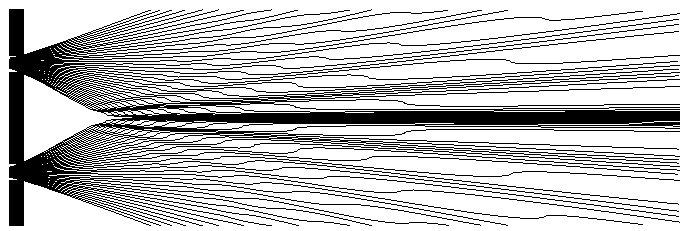
\includegraphics[width=.94\linewidth]{figures/ch08_fig01.pdf}
\caption{二重スリット実験で粒子がたどり得るBohm軌道の一例。Springer Science and Business Mediaのご厚意により、許可を得て\cite{ref480}から転載。}
\end{figure}

Bohm力学では、波動関数は「誘導場」の役割を果たす。すなわち、誘導方程式(8.9)を通じて、波動関数が、粒子が従う速度場を生成する。したがってBohm理論は、Newton力学と同様、軌道に沿う粒子の運動を記述する。しかし、古典力学の力と加速度の法則の代わりに、粒子の運動方程式は今や(8.9)で与えられ、その右辺に入る波動関数$\psi$の変化は、Schrödinger方程式で定まる。

この形式は、二重スリット実験の文脈で明快に示せる\cite{ref037,ref481}。図8.1は、スリットの後方で単一粒子が取り得るBohm軌道の集合を示す。各粒子は、これらの確定した軌道の一つをたどり、したがってスリットの一方を通過する。個々の粒子がどのBohm軌道を取るかは、単にその粒子の初期位置に依存する。したがって、各粒子が、与えられた任意の時刻に同じ波動関数$\psi$で記述されても、粒子は決定論的に異なる確定した軌道をたどる。ゆえにBohm力学は、隠れた変数理論の一例である（2.1.2節参照）。つまり、波動関数$\psi$は系の物理状態の完全な記述ではなく、粒子の常に確定した位置$\boldsymbol q_i(t)$が、隠れた変数の役割を果たす。図8.1を見ると、粒子は明確に非Newton的な経路を取る。粒子軌道は直線ではなく、波動関数$\psi$の振幅が大きい領域に集中する。したがって、スクリーン上で観測される、おなじみの干渉模様の極大と極小を、Bohm軌道の「密度」に直接結びつけることができる。


% 原文 p.356
\hypertarget{srcpage:356}{}\label{srcpage:356}
\subsubsectionlink{基本的実体としての粒子}
Bohm理論は、粒子に基本的な存在論的地位を与えることで批判されてきた。相対論的量子論の根本的な水準で粒子を認めることに反対する、一般的な議論は、しばしばなされている（たとえば\cite{ref482,ref483}参照）\footnote{他方、「量子場のBohm力学」、すなわち量子場の理論をBohm型の枠組みに組み込む理論の提案もある\cite{ref484,ref485}。}。さらに、本節で論じたい点であるが、粒子の現れは連続的なデコヒーレンス過程から導けると論じられ、その結果、粒子に基本的役割を与える必要はないとも主張されている\cite{ref408,ref486,ref487}。中間的尺度や巨視的な系のデコヒーレンスした縮約密度行列が、本質的に常に、位置空間の狭い波束の非真正集団を表すことに基づき、Zeh\cite[190頁]{ref408}は、そのような波束を、個々の「粒子」の位置を表すものとみなせるとする。
\begin{quote}
量子場の測定で観測される粒子的側面（乾板上の点、泡箱中の飛跡、計数器のクリックなど）はすべて、関係する局所的、すなわち部分系の密度行列の、このデコヒーレンスを考慮することによって理解できる。
\end{quote}
もちろん、デコヒーレンスから得られる狭い波束の非真正集団が、個々の粒子の知覚をもたらすと解釈するためには、波束の一つだけが知覚される理由を説明する、追加の解釈の枠組みを与えなければならない。すなわち、デコヒーレンスから生じる非真正集団から個々の項の知覚へ至るためには、何らかの解釈規則を加える必要があり、それゆえ、デコヒーレンスだけで必ずBohmの粒子概念が不要になるわけではない。しかし、基本的実体として粒子を仮定することは不要かもしれないと示唆される。そして、そのような粒子理論を相対論的量子場理論と両立させる困難も考え合わせると、理論の基本的水準に粒子を先験的に仮定するBohmの立場は、重大な挑戦を受けているように見える。

\subsubsectionlink{Bohm軌道とデコヒーレンス}
Bohm力学のよく知られた性質は、その軌道がしばしば著しく非古典的になることである（たとえば\cite{ref037,ref488,ref489}参照）。これは、巨視的水準での準古典的軌道の存在を、Bohm理論がどのように説明できるのかという、重大な問題を生む。


% 原文 p.357
\hypertarget{srcpage:357}{}\label{srcpage:357}
BohmとHiley\cite{ref037}は、巨視的な系による環境粒子ビームの散乱を考えた。この過程はデコヒーレンスを生じさせる\cite{ref007,ref017}。彼らは、この散乱が系の準古典的軌道をもたらすことを示した。またAppleby\cite{ref489}は、孤立系については、Bohm理論は一般に正しい古典極限を与えないことを示した。そこで、環境と、それによるデコヒーレンス効果を含めることが、Bohm力学で準古典的軌道を回復するために役立つかもしれないと提案された\cite{ref486,ref490,ref491,ref492,ref493,ref494}。基本的考えは、デコヒーレンスが作り出す非真正集団における準Newton的な位相空間軌道（たとえば5.2.5節参照）を、Bohm理論の粒子軌道$Q(t)$と結びつけることである。Bacciagaluppi\cite{ref391}が指摘したように、この方法の大きな利点は、同じ方法で量子現象と古典現象の両方を回復できることである。

しかし、Appleby\cite{ref490}の注意深い分析は、デコヒーレンスをもたらす過程が巨視的な系の正しい準古典的Bohm軌道ももたらすのは、ある追加の仮定の下だけであることを示した。Applebyは、初めにエネルギー固有状態に準備された系の、長時間極限の例を述べた。Allori\cite{ref491}、AlloriとZanghì\cite{ref492}、Alloriら\cite{ref493}も、興味深い結果を報告している。これらの著者は、デコヒーレンス効果が、Bohm軌道の古典的性質を保存する役割を果たし得ることを示した。さらに、標準量子力学では、古典性の出現を説明するために狭い波束を維持することが重要であるのに対して、波動関数と配置の両方によるBohm的な系の記述では、高度に非局在化した波動関数から、準古典的振る舞いを導けることを示した。

SanzとBorondo\cite{ref494}は、Bohm力学の枠組みで、デコヒーレンスがある場合の二重スリット実験を調べた。空間的コヒーレンスが完全に失われ、したがって干渉がなくなっても、Bohm理論における粒子の動力学へ影響する非局所的量子相関が残ることを示した。この例は、一般には、デコヒーレンスだけでは、Bohm力学の正しい古典極限を保証するには十分でないことを示している。

\subsectionlink{まとめ}
本章では、各解釈における「確定した量」の、非常に一般的で経験的に適切な定義と説明を実現するため、優先状態の環境誘起超選択が、量子力学の異なる解釈へどのように組み込まれてきたかを示した。
% 原文 p.358
\hypertarget{srcpage:358}{}\label{srcpage:358}
こうして、デコヒーレンスの研究計画は、多くの解釈を長く悩ませてきた悪名高い優先基底問題の解決に、非常に大きな貢献をした。相対状態解釈のような場合には、優先基底の明確な定義がないことが、そのような解釈に対する継続的批判の中心であった。物理的収縮理論やBohm力学のような場合には、優先基底の具体的な形が単に仮定されている。この場合、デコヒーレンスは、仮定される量の特定の選択に、物理的動機を与えることができる。

量子力学の標準解釈の中では、デコヒーレンスは量子測定の結果の問題を解決できないと論じた。私たちには依然として、多数の成分が残される。各成分がよく局在した準古典的なものであるとしても同じである。そして、単一の結果が知覚される理由と仕方を説明するためには、この状況に何かを補うか、あるいは解釈する必要がある。したがって、結果の知覚と一般的な古典性を説明するため、固有値・固有状態リンクを変えたり完全に捨てたり、ユニタリー動力学を修正したりする別の解釈的方法の規則や仮定に、物理的動機を与え、あるいはそれらを反証するために、環境誘起超選択と干渉項の局所的抑制を、大いに利用できることを論じた。

たとえば、その応用のいくつかだけを挙げると、デコヒーレンスは、相対状態解釈における分枝選択の普遍的基準と、観測者の視点から見た分枝間の非干渉についての物理的説明を与えられる。様相解釈では、系へ割り当て得る、経験的に適切な性質の集合を指定するために使える。収縮模型では、自由パラメーター、そしておそらくは縮約機構自体の性質さえも、環境相互作用から導けるかもしれない。Bohm力学で準古典的な粒子軌道を選ぶ助けにもなる。さらに、デコヒーレンスは、異なる解釈の経験的適合性、したがって経験的等価性を保証し得ることが明らかになった。この点から、物理学者Max Tegmarkは、たとえば正統的解釈とEverett解釈の選択が、「純粋に好みの問題となり、おおよそ、数学的言語と人間の言語のどちらを、より根本的だと信じるかに等しくなる」\cite[855頁]{ref495}かもしれないと提案した。


\clearpage
\setcounter{section}{8}
\setcounter{footnote}{0}

% 原文 p.359
\hypertarget{srcpage:359}{}\label{srcpage:359}
\sectionlink{観測、量子的な脳、デコヒーレンス}
\setcounter{footnote}{0}

生物系が量子力学的な言葉で分析されることは、めったにない。そのような系の途方もない複雑さのため、量子力学的に扱うことは本質的に不可能である。さらに、生物系の構造は通常、室温の水性環境に埋め込まれている。したがって、そのような系には非常に強いデコヒーレンスが働き、量子コヒーレントな振る舞いを実効的に抑制すると予想するのが合理的である。同時に、量子力学があらゆる尺度で妥当だと考えるなら、生物構造の振る舞いは量子力学の法則に従う。

この文脈で、脳は特に興味深い生物系である。それは私たちの知覚を処理する中枢の器官をなす。物理理論の経験的に意味のあるあらゆる言明は、まさにこれらの知覚に関係づけられなければならないことは明らかである。したがって、理論の予測に基づいて私たちの観測を説明しようとするとき、これらの知覚を私たちへもたらす系、すなわち脳の役割を説明する必要があるかもしれない。さらに、以下で概説するように、歴史的には、量子論における「意識」の役割という関連する問題も生じており、意識が波動関数の収縮を誘起するかもしれないという提案もなされてきた。

本章では、量子力学における観測の一般的問題について、いくつかの導入的考察を行った後（9.1節）、9.2節で、von Neumannの測定図式（2.5.1節参照）に観測者を明示的に含め、その帰結を論じる。続いて、量子力学的な脳に焦点を当てる（9.3節）。脳内のニューロンや、ほかの構造の重ね合わせ状態のデコヒーレンス特性を模型化した研究をいくつか述べる。それらからは、関係するデコヒーレンス時間尺度の具体的な数値評価が得られている。9.4節では、これらの結果が、測定問題の「主観的」解決に対して持つ含意も、簡単に論じる。

\subsectionlink{量子力学における観測者の役割}
量子力学における観測者の役割は、理論の初期にまでさかのぼる、多くの基礎論争の核心にあった。古典物理学とは対照的に、状態が本質的に壊れやすいという事実が、量子力学の特異な特徴であることを思い出そう（2.1節参照）。
% 原文 p.360
\hypertarget{srcpage:360}{}\label{srcpage:360}
ある特定の物理量の測定は一般に、系の量子状態を乱し、それゆえ非可換な観測量で表される、別の物理量の後続の測定結果を乱す。

したがって、系の物理状態は、観測者が測ることを選ぶもの、そのもので「ある」ように見える。この特徴は、古典理論ではほとんど知られていない「主観性」の色合いを、自然の記述へ持ち込む。ゆえに、観測、したがって観測者は、古典物理学におけるよりも、量子力学でははるかに根本的な役割を果たすように見える。「粒子の軌道は、私たちがそれを観測する行為によって作られる」\cite[185頁]{ref042}というHeisenbergの急進的な言明を、すでに引用した（原著19頁参照）。Bohrの著作に最も明瞭な、この実証主義的な見方では、量子力学の形式全体は本質的に、測定が行われた場合に、観測者が何を見いだすかを予測する処方箋をなす。しかし、「外部に実際には何があるか」について、存在論的主張は何も行わない。実際、Copenhagen解釈では、測定前の系の物理状態についての言明は、すべて無意味とされる。

実験物理学の実用的な問題を扱う際には、Copenhagen解釈の何らかの変種を採用する多くの人々でさえ、量子力学が指示すべき、観測者に依存しない物理的実在の存在を信じ続けている。そこで中心となる問いは、物理系には一般に、測定前の物理量の値の完全な組を割り当てられない、という量子力学から学んだ教訓を、理論が何らかの仕方で関係してほしいと願う、私たちを取り巻く「客観的に存在する」世界への、直観的に感じられる必要性と、どう両立させるかである。

同時に、私たちは、単に主観的知覚の産物かもしれないにもかかわらず、客観的であり、したがって物理理論に必須の一部だとみなすようになった概念も、注意深く吟味することを迫られる。von Neumann\cite[第VI章]{ref060}は、次のことを思い起こさせた。
\begin{quote}
経験が述べるのは、「ある観測者が特定の主観的観測を行った」という種類の言明だけであり、「ある物理量が特定の値を持つ」という種類の言明では決してない\footnote{ドイツ語原文は次のとおりである。``Denn die Erfahrung macht nur Aussagen von diesem Typus: ein Beobachter hat eine bestimmte (subjektive) Wahrnehmung gemacht, und nie eine solche: eine physikalische Größe hat einen bestimmten Wert.''}。
\end{quote}
同様に、d'Espagnat\cite[134--135頁]{ref496}は、次のように注意を促す。
\begin{quote}
私たちが、別々の場所にある巨視的物体というような「もの」を知覚するという事実は、少なくとも部分的には、私たちの感覚と知性の装置の構造による。したがって、それを、量子状態を定義するために考慮しなければならない、確かな知識の総体の一部とみなすべきではない。（中略）実際、科学の目的は、人間の経験を記述することであって、「実際にあるもの」を記述することではない、と科学者が主張するのは、まったく正しい。そして、人間の経験を記述したいだけである限り、すなわち、すべての可能な状況で何が観測されるかを予測できることで満足する限り、（中略）通常の三次元空間の確定した場所に、観測されていない、すなわちまだ観測されていない物体が、何らかの絶対的意味で存在すると仮定する必要はない。
\end{quote}

% 原文 p.361
\hypertarget{srcpage:361}{}\label{srcpage:361}
したがってvon Neumannとd'Espagnatは、一般的で客観的な「確定性」に対する、しばしば深く感じられるこだわりが、巨視的な系についての日常経験だけに基づいていることを認識するよう促している。もし経験とは独立に、確定性が自然界に実際に存在することを知ることができるなら、「外部」の物理現象を「内部」の知覚・認知装置へ結びつける単純な模型を作りさえすれば、主観的確定性は、おそらく客観的確定性の帰結になるだろう。その模型が単純であると予想する根拠としては、外部過程と内部過程を支配する物理法則が同一だという想定を挙げられる。von Neumannは、この仮定を「心身並行論」\cite{ref060}と呼んだ。しかし、どの知識も直接または間接に観測に基づくので、確定性の客観的存在についての知識を、私たちの主観的な確定性の観測に根ざさせずに得る方法はない。同時に、巨視的な干渉・コヒーレンス現象は、量子世界と、直接経験の水準で観測される確定性との境界が、曖昧であることを明瞭に示している（第6章参照）。

したがって、満足のいく物理理論には、客観的確定性が先験的な一部として含まれるべきだという要求を捨てることも、実際には合理的かもしれない。もちろん、その理論が、私たちが主観的に観測するすべての確定性を、経験と一致するように説明できることが条件である。それに対応する測定問題の「主観的」解決は、デコヒーレンス理論から大きな後押しを受けてきた。実際、デコヒーレンスは、この種の主観的方法の多くを、そもそも経験的に成立可能にする。全体の水準で確定性を強制しなくても、局所観測者の視点から確定性を導けるかもしれないからである。後の9.4節で、このような方法をより詳しく論じる。

\subsectionlink{量子的観測者とvon Neumann連鎖}
Copenhagen解釈（8.1節）や、ほかの量子力学の解釈のように、測定と観測者へ特定の先験的役割を与える代わりに、ここでは異なる視点を取ろう。観測者を単に、観測対象の系と相互作用する量子系として扱う。この状況は、2.5.1節で論じたvon Neumannの測定図式を用い、観測者を、測定相互作用のvon Neumann連鎖における最後の環として含めて模型化できる（図9.1）。


% 原文 p.362
\hypertarget{srcpage:362}{}\label{srcpage:362}
\begin{figure}[htbp]
\centering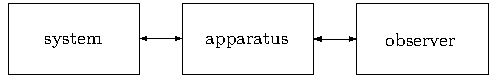
\includegraphics[width=.88\linewidth]{figures/ch09_fig01.pdf}
\caption{最後の環として観測者を含めたvon Neumann連鎖。}
\end{figure}

このとき、測定の異なる可能な結果を観測することに対応する、観測者の量子状態は、測定装置の対応する相対状態と量子的に相関する。さらに装置は、対象の系を記述する重ね合わせ状態の異なる成分と量子的に相関する。この測定相互作用を、通常のvon Neumannの形で模式的に表すと、次のようになる［(2.54)参照］。
\begin{equation}
\begin{aligned}
&\Bigl(\sum_n c_n|n\rangle\Bigr)|\text{装置準備完了}\rangle|\text{観測者準備完了}\rangle\\
&\quad\longrightarrow\sum_n c_n|n\rangle|\text{指針は }n\rangle|\text{観測者が結果 }n\text{ を知覚}\rangle .
\end{aligned}\tag{9.1}
\end{equation}
ここで$\sum_n c_n|n\rangle$は、観測、すなわち測定される系の状態である。したがって、この形式で測定を記述する最終量子状態は、系・装置・観測者がもつれた重ね合わせ状態であり、その各成分は、測定の異なる「結果」に対応する。

しかし、(9.1)のように観測者を含めても、相互作用する系のvon Neumann連鎖は終わらない。この連鎖に、環境、二次的装置や観測者など、さらに環を付け加えると、(9.1)と同様に、可能なすべての結果に対応する状態を含む、もつれた最終状態へ再び至る。これらの環をすべて含む複合系の時間発展が厳密にユニタリーである限り、この状態に含まれる情報量、たとえば純粋度やvon Neumannエントロピー（2.4.3節参照）で測られる情報量は変化できず、連鎖は終わらない。ゆえに、私たちは無限後退の問題に直面する。

ここから、これらの異なる相関した成分状態が、観測者が実際に経験する単一の測定結果へ、どのように、いつ縮約し得るのかという、根本的な問いが生じる。von Neumann連鎖が終わるのか、どのように、どこで終わるのかという問題は、もちろん本質的には結果の問題であり、本書のいくつかの箇所ですでに論じてきた（たとえば2.5.4節と8.1節参照）。von Neumann自身も、この問題を明確に認識していた。彼にとって唯一確かな事実は、観測者である私たちが、測定の終了時には常に確定した結果を知覚することだった。したがって理論は、少なくとも観測者の経験の水準で、そのような確定した知覚を説明しなければならない。量子力学の統計的予測は、観測連鎖のどこにHeisenberg切断を置くかに依存しない。
% 原文 p.363
\hypertarget{srcpage:363}{}\label{srcpage:363}
したがって、何らかの形の波動関数の収縮を、装置と観測者の間の、どの段階にも導入できる。しかし、明白な経験的制約によって、明らかに確定した結果を知覚することの説明が、実際に不可避となるのは、観測者の水準においてだけである。

この精神に沿って、von Neumannは観測者の内部での波動関数の収縮を仮定し、それを「第一の介入」（ドイツ語で``erster Eingriff''）と呼んだ\footnote{興味深いことに、系・装置・観測者の相互作用を支配するユニタリーなSchrödinger発展は、「第二の介入」と呼ばれた。}。この方法は、Copenhagen解釈（8.1節参照）と著しく対照的だった。後者では、量子力学的にそれ以上分析すべきではない、本質的に古典的な測定装置の存在という仮定の中に、波動関数の収縮が暗黙に含まれていたのに対して、von Neumannは、測定装置自体に特別な役割を与えなかった。しかし、相互作用する量子系という純粋に量子力学的な形式から、確定した結果の知覚をどう説明するかという問題を解決できず、彼は、基本的な量子・古典境界を維持せざるを得ないと感じた。ただし、その境界を今や観測者にまで押し進めたのである。したがって、測定過程を純粋に量子力学的に記述しようというvon Neumannの野心的目標は、観測者の水準での収縮を恣意的に導入したことで、途上で打ち切られたといえる。

von Neumann自身は、観測者における収縮の本性や、測定装置のような無生物と観測者とを何が区別するのかについて、詳しく述べなかった。しかし、Heisenberg切断を観測者の中に置くことによって、新たな扉が開かれた。すなわち、量子測定過程と、実際の、あるいは単に知覚されるだけの波動関数の収縮における、「意識」の役割という問いである。

物理理論の基本的水準に「心」や「意識」といった、かなり曖昧な言葉を含める方法は、確かに自然科学一般、特に物理学の伝統的方法に反する。同時に、量子論における観測者の特異な重要性、すなわち、私たちが直接観測する世界と同様の構造を持つ、観測者に依存しない実在という、それまで疑われなかった仮定から離れなければならないように見えることは、観測者の心に特別な物理的役割を与える考えを、再導入したように見える。

Copenhagen解釈自体と、そこに体現された実証主義的態度さえも、量子力学を本質的に、観測者による検証、すなわち測定の文脈で初めて物理的意味を得る言明の組とみなすことによって、「心」という概念に暗黙に重要性を与えている。d'Espagnat\cite{ref497}が論じたように、「ある」ものではなく、観測者が「見いだせる」ものだけに言及することによって、検証し、見いだす観測者の心が、科学的実在に先立つ原始的な概念をなす。
% 原文 p.364
\hypertarget{srcpage:364}{}\label{srcpage:364}
しかし、「心」や「意識」のような言葉は、Copenhagen解釈の明示的な一部ではなかった。また、観測者が得る知識は、それでも何らかの基礎的な物理的実在に関係しなければならない、という基本的直観を、この解釈の支持者は本当に捨てたわけではなかった。

意識が量子測定過程で基本的役割を果たすという考えの、有名な、ただし一時的な支持者にEugene Wignerがいた。彼の動機は、1960年代初頭に考案し、その後「Wignerの友人」の問題として知られるようになった思考実験\cite{ref498}に基づいていた。この思考実験は、Schrödingerの猫の設定を変えたものである。毒を、不安定な原子が崩壊すると閃光を発する測定装置に置き換え、決定的なこととして、猫を「Wignerの友人」と呼ばれる人間の観測者で置き換える。友人と区別するため、元のSchrödingerの猫の設定における外部観測者を、「Wigner」と呼ぼう。

したがって、この設定には二人の人間の観測者が含まれる。一人は、原子と装置の系との測定型相互作用が、von Neumann図式で量子力学的に記述される「内部」の観測者、すなわちWignerの友人である。もう一人は、後になってこの相互作用の結果を尋ねる「外部」の観測者、すなわちWigner自身である。猫、不安定な原子、毒を入れた元の猫の設定の箱は、ここでは原子、測定装置、Wignerの友人を含む実験室に対応する。Wignerは、しばらく実験室の外で待つ。その間に、原子・装置・Wignerの友人の結合状態は、通常の猫型の重ね合わせへ発展する。この発展を、模式的に次の形で表せる。
\begin{equation}
\begin{aligned}
&(\alpha|\text{原子未崩壊}\rangle+\beta|\text{原子崩壊}\rangle)
\otimes|\text{装置準備完了}\rangle|\text{観測者準備完了}\rangle\\
&\quad\longrightarrow\alpha|\text{原子未崩壊}\rangle|\text{閃光なし}\rangle|\text{閃光を観測せず}\rangle\\
&\qquad\quad+\beta|\text{原子崩壊}\rangle|\text{閃光あり}\rangle|\text{閃光を観測}\rangle .
\end{aligned}\tag{9.2}
\end{equation}
その後Wignerは、実験の結果を尋ねるために部屋へ入る。彼は友人に、閃光を見たかどうか尋ねる。友人は明らかに、閃光を観測したか、観測しなかったかの、どちらかを答える。その答えに応じてWignerは、自分の視点からは、原子・装置・友人の結合系を記述する猫状態が、(9.2)の右辺の二成分の一方へ収縮したと結論するだろう。しかし、彼が実験室へ入って最初の問いを発する前の、閃光に関する経験を尋ねたら、Wignerの友人は何と答えるだろうか。

本質的には、Schrödingerの猫の設定の場合と同様、Wignerの友人の例が浮き彫りにする中心的問題は、収縮を誘起する測定が、いつどこで行われるかという問いである。
% 原文 p.365
\hypertarget{srcpage:365}{}\label{srcpage:365}
ただし、Wignerの友人の場合には、Schrödingerの猫の逆説との違い、そしてWignerの考えでは決定的な違いは、重ね合わせが意識ある観測者を含むことである。この観測者は、Wignerが実験室へ入って閃光を見たかどうかを尋ねる前の経験について、彼が部屋に入った後、言葉による報告を与えられるはずである。

Wigner自身は、(9.2)の二つの異なる「意識状態」、すなわち閃光の観測に対応する状態と、閃光を観測しない状態の重ね合わせは、不合理だとみなさなければならないと考えた。彼の意見では、意識ある観測者は、常にこれらの状態の一つだけにいなければならなかった\cite{ref498}。この信念から彼は、意識的観測は(9.2)のような標準的な線形量子形式では記述できないと結論した。すなわち、意識は、ユニタリー発展を破り、意識ある観測者の確定した状態への波動関数の収縮を誘起するという意味で、物質的対象と根本的に異ならなければならないとした。

純粋に経験的な観点からは、Wignerの推論の決定性に対する強い反論がある。異なる意識状態の重ね合わせは、これらの状態がいかなる仕方でも干渉しない限り、すなわち意識ある観測者の異なる「量子的版」が互いを「意識」しない限り、必ずしも不合理とみなして排除する必要はない、ということである。デコヒーレンスは、意識ある観測者にも避けがたく影響する。したがって、観測者の「内側からの見方」では、(9.2)の異なる「意識の分枝」の存在を、経験的に確認することはできないだろうと推測できる。この点は、9.4節でより詳しく論じる。実際Wignerは、デコヒーレンス研究の基礎となる考えのいくつかを導入した、Zehの1970年の論文\cite{ref004}を知ると、後に、量子測定における意識の特別な役割という見解を捨てた\cite{ref499}。

\subsectionlink{脳におけるデコヒーレンス：脳は量子コンピューターか}
脳は、$O(10^{11})$個のニューロンが$O(10^{14})$個のシナプスで相互接続された、驚くほど複雑なネットワークからなる。この神経回路網の記憶能力と動的相互作用が、感覚入力の保存と処理の生理学的核心であることを示す、説得力ある議論がある。「意識」の知覚を含む、すべての認知過程が、最終的にはニューロン活動へ還元できると推測することは、不合理ではない。神経生物学や生物物理学の研究者は、脳を通常、オン・オフの「スイッチ」（節点）が大規模に並列接続された網として、完全に古典的な言葉で模型化する\cite{ref500,ref501,ref502}。各節点は単一のニューロンを表し、特定の、しばしば非線形な活性化関数に応じてオンまたはオフとなり、それぞれニューロンの発火状態と静止状態に対応する。明白な理由から、このような模型は通常、人工神経回路網と呼ばれる。


% 原文 p.366
\hypertarget{srcpage:366}{}\label{srcpage:366}
大まかにいえば、このように脳は古典コンピューターとして模型化される。そのような模型研究から得られた意外な知見の一つは、比較的少数の節点と、各節点の活性化に関するごく少数の規則だけに基づく、比較的単純なネットワークでさえ、単純な認知過程で観測されるものに似た、驚くほど複雑な振る舞いを生み出せることである。しかし、このような古典模型の成功にもかかわらず、量子効果が私たちの認知装置で重要な役割を果たすかどうかは、少なくとも二つの観点から論じられてきた。

第一に、量子的な「不確定性」と、量子力学の見かけ上の非決定性を持ち出して、古典物理学が要請する厳密な決定論を回避し、「自由意志」という概念を回復しようとすることがある。しかし、この方法には根本的な誤りがある。どのような量子的「不確定性」も、まったく制御不可能な効果を表すはずであり、自分の行動を能動的に制御し決定できるという感覚に基づく、「自由意志」の理解とは完全に異なる。同じ理由で、量子力学が測定結果の確率だけを予測し、それゆえ物理世界の記述に非決定性を再導入するように見えるという事実から、自由意志の存在を推論することはできない。繰り返せば、そのような「量子的ランダムさ」が引き起こす行動は、自由意志を持つとされる個人には制御できない。したがって、このように量子論を持ち出すことは、何かをもたらすとしても、古くからの「自由意志の問題」を、もしそれがそもそも問題であるなら、いっそう深刻にするだけである\footnote{自由意志について、Einsteinは1932年の思索的な『Credo』\cite{ref503}で、かつて次のように述べた。「私は自由意志を信じない。Schopenhauerの『人は自分の欲することを行うことはできるが、自分の欲することを欲することはできない』という言葉は、生涯のあらゆる状況で私に付き添い、他人の行いが私にとってかなり苦痛であるときでも、それを受け入れさせてくれる。自由意志がないと知ることは、行動し判断する個人としての自分自身や同胞を、あまり深刻に受け取りすぎたり、平静を失ったりすることから、私を守ってくれる。」原文は次のとおりである。``Ich glaube nicht an die Freiheit des Willens. Schopenhauers Wort: `Der Mensch kann wohl tun, was er will, aber er kann nicht wollen, was er will', begleitet mich in allen Lebenslagen und versöhnt mich mit den Handlungen der Menschen, auch wenn sie mir recht schmerzlich sind. Diese Erkenntnis von der Unfreiheit des Willens schützt mich davor, mich selbst und die Mitmenschen als handelnde und urteilende Individuen allzu ernst zu nehmen und den guten Humor zu verlieren.''}。最後に、脳内のシナプス伝達には、その基礎にある生物過程の複雑さのために、かなり高い失敗率があることにも注意すべきである\cite{ref504}。これによって、「日常の水準」で、かなり高い予測不可能性が必然的に生じる。このような純粋に機能的な予測不可能性は、どのような量子的不確定性の効果よりも、おそらくはるかに重要である。したがって、予測可能な入出力パターンを持つ、決定論的な古典コンピューターとして脳を見ることは、実際にはあまり文字どおりに受け取るべきではない。


% 原文 p.367
\hypertarget{srcpage:367}{}\label{srcpage:367}
量子論を脳へ適用するこの「素朴な」考えを超えたところには、脳が生み出す人間の認知過程の複雑さは、脳が量子コンピューターとして働くことができる場合にだけ説明できるかもしれない、という提案の領域がある。言い換えれば、こうした提案は、脳の能力の少なくとも一部が、脳内の通常の古典状態、たとえばニューロンの静止状態と発火状態の、量子コヒーレントな重ね合わせの存在と操作によるかもしれない、という考えに基づく。もしこれが正しければ、古典的な人工神経回路網では、脳を完全にシミュレートするには本質的に不十分だということになる。

特に、人間の意識が量子コヒーレントな過程に結びついているかどうかは、しばしば論じられてきた。前の9.2節では、関連しているが向きの逆の概念、すなわち意識の作用が波動関数の収縮を引き起こすかもしれないという、Wignerの初期の推測\cite{ref498}に、すでに触れた。そこでは、測定型相互作用のvon Neumann連鎖によって作られた、全体のもつれた状態(9.1)に含まれる量子コヒーレンスを、実効的に破壊するために意識が持ち出された。今や問題の向きは逆である。量子コヒーレンスは、意識の出現に結びついているのだろうか。この文脈では、さまざまな巨視的量子コヒーレント過程が、意識の起源として提案されてきた（たとえば\cite{ref505,ref506,ref507,ref508,ref509,ref510,ref511}参照）。特に著名なのは、Penrose\cite{ref473}たち\cite{ref512,ref513,ref514}による提案である。彼らは、細胞骨格、すなわち細胞内部の足場の主要部分をなす、動的に活動する構造である、脳内のいわゆる微小管が、量子計算を可能にするほど長いデコヒーレンス時間を持つかもしれず、さらに、その計算が意識の出現と結びつくかもしれないと提案した（後の9.3.2節参照）。

意識というかなり曖昧な概念や、基礎物理理論におけるその役割の可能性に関する問題とは、まったく独立に、ここで論じるべき明白な中心的問いは、次のものである。脳内の関係する構造、特にニューロンと微小管は、脳内で量子計算を実行できるほど長く、量子コヒーレンスを維持できるだろうか。本書の前の章でのデコヒーレンスの議論に基づけば、そのようなデコヒーレンス時間は極めて短いと予想するだろう。結局、ニューロンと微小管は、生物学的尺度では小さくても、量子物理学で通常考える尺度では、依然として巨視的で非常に複雑な物体である。たとえばニューロンが発火と静止の重ね合わせにある状態は、巨視的に異なる状態の重ね合わせという分類へ、明らかに入る（以下参照）。さらに、これらの構造は、巨視的な「暖かく湿った」環境に埋め込まれ、その環境と強く相互作用している。

デコヒーレンス時間の短さについてのこの直観は、Tegmarkが2000年に報告した定量的結果\cite{ref515}によって支持された。Tegmarkは、ニューロンと微小管が脳内の自然な環境と相互作用する模型を考え、これらの構造における重ね合わせ状態のデコヒーレンス時間尺度について、桁の評価を示した。
% 原文 p.368
\hypertarget{srcpage:368}{}\label{srcpage:368}
以下の9.3.1節でニューロンのデコヒーレンスを、9.3.2節で微小管のデコヒーレンスを扱い、これらの結果を述べる。測定問題の「主観的」解決に対する含意は、9.4節で論じる。

\subsubsectionlink{ニューロンの重ね合わせ状態のデコヒーレンス時間尺度}
まずTegmark\cite{ref515}が考えた、ニューロンのデコヒーレンスを論じよう。ここで関心のあるニューロンの主要部分は、いわゆる軸索である。これは、直径約$d\approx10\,\mu\mathrm m$の、長い中空の管と考えられる（図9.2）。軸索壁の大部分は、絶縁体として働くミエリンで覆われている。しかし、軸索に沿って、この絶縁がない幅数nmの狭い帯があり、厚さ約$h\approx10\,\mathrm{nm}$の半透膜の領域を形成する。そこでは、軸索の内部と、それを取り囲む水性媒質との間で、イオンが交換される。ニューロンの発火は、膜内に位置する電位依存性Naチャネルを介して、周囲からこれらの膜領域を通り、軸索内部へNaイオンが非常に急速に流入することによって表される。この発火は、軸索に沿って最大$100\,\mathrm{m/s}$という高速で伝播し、各領域のNaチャネルを開く。イオンの流入は約1msしか続かず、その後Naチャネルは再び閉じ、ニューロンは静止状態へ戻る。中枢神経系に見られるニューロンの典型的パラメーターを使い、Tegmarkは、発火中に、個々の膜領域すべてからの寄与を合わせた軸索膜全体を、合計$O(10^6)$個のNaイオンが横切ると見積もった。

\begin{figure}[htbp]
\centering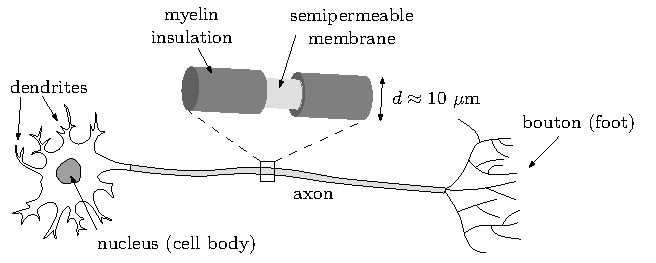
\includegraphics[width=.94\linewidth]{figures/ch09_fig02.pdf}
\caption{ニューロンの模式図。説明を明瞭にするため、軸索の一部分を拡大している。軸索壁の大部分はミエリンで覆われ、軸索内部を周囲の媒質から絶縁している。しかし、小さな帯状領域にはこの絶縁がなく、そこにある半透膜をイオンが通り抜けられる。}
\end{figure}

これは、発火中には静止中より、軸索内部に$N=10^6$個程度多くのNaイオンがあることを意味する（図9.3参照）。
% 原文 p.369
\hypertarget{srcpage:369}{}\label{srcpage:369}
したがって、発火状態と静止状態の重ね合わせは、$O(N)$個のNa原子の集まりが、それぞれ軸索の内部と外部に位置する二つの状態の重ね合わせに対応する。言い換えれば、$O(N)$個のNa原子からなる系を扱っており、それは$O(h)$の距離だけ離れた二つの重心位置の重ね合わせで記述される。

\begin{figure}[htbp]
\centering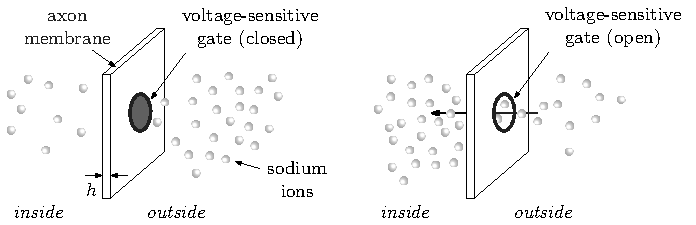
\includegraphics[width=.94\linewidth]{figures/ch09_fig03.pdf}
\caption{ニューロンの静止状態（左）と発火状態（右）。発火状態では、静止状態よりも$O(10^6)$個多くのNaイオンが軸索内部に存在する。}
\end{figure}

Tegmarkは次に、ニューロンの重ね合わせがコヒーレンスを失う、三種類の環境相互作用を調べた。すなわち、近くのNaイオンおよびKイオンとNa原子との衝突、周囲の水分子との衝突、離れたイオンとの静電的、すなわちCoulomb相互作用である。三つの場合はすべて、第3章で述べた散乱によるデコヒーレンスの理論を用いて扱える\footnote{第3章で作った模型は、散乱体、すなわち対象の系の運動量変化が、散乱される環境粒子の運動量変化に比べてはるかに小さく、物体の反跳を無視できるという仮定に基づいていることに注意しよう。厳密には、ここではこの近似は成り立たない。散乱体であるNaイオンの質量が、環境粒子であるNaイオン、Kイオン、水分子の質量と同程度だからである。したがって、以下の数値評価をあまり文字どおりに受け取るべきではない。他方、現在の目的には、いくつかの粗い評価で満足することにする。正しい値が、この評価から数桁ずれていても、ニューロンのこのような重ね合わせ状態のデコヒーレンス時間尺度が、生物学的・認知的過程に関係する時間尺度に比べて極めて短い、という一般的結論には影響しない。}。イオン同士の衝突と、イオンと水の衝突という、最初の二つの場合の考え方を、簡単に概説しよう。$T=310\,\mathrm K$、すなわち人間の体温における、NaイオンまたはKイオンと水分子の熱的de Broglie波長(2.114)は同程度で、$\lambda_{\mathrm{dB}}\approx0.03\,\mathrm{nm}$である。この値は、コヒーレントな空間的隔たり$h\approx10\,\mathrm{nm}$に比べてはるかに小さい。これは、散乱される環境粒子として働くイオンや水分子が、隔たり$h$を完全に分解できることを意味する。したがって、3.3.1節で論じた短波長極限に、完全に入っている。


% 原文 p.370
\hypertarget{srcpage:370}{}\label{srcpage:370}
デコヒーレンスが最大となるこの極限で、系の位置空間縮約密度行列の非対角要素の減衰率は、全散乱率$\Gamma_{\mathrm{tot}}$が定める値で飽和することを示した［(3.48)参照］。
\begin{equation}
\rho(x,x',t)=\rho(x,x',0)e^{-\Gamma_{\mathrm{tot}}t}.\tag{9.3}
\end{equation}
軸索の内側と外側にある重ね合わせ状態の、単一Naイオンについて、TegmarkはCoulomb散乱断面積を用い、NaイオンおよびKイオンとの衝突に対して$\Gamma_{\mathrm{tot}}\approx10^{14}\,\mathrm{s}^{-1}$、水分子の散乱に対してもほぼ同じ値と評価した。したがって、$N=10^6$個のイオンを含む空間的重ね合わせのデコヒーレンス時間尺度$\tau_{\mathrm d}$は、
\begin{equation}
\tau_{\mathrm d}=(N\Gamma_{\mathrm{tot}})^{-1}\approx10^{-20}\,\mathrm s\tag{9.4}
\end{equation}
程度と見積もられる。

より遠くのイオンとのCoulomb相互作用によるデコヒーレンスという第三の場合にも、Tegmarkは同様の散乱模型を使った。ここでは詳細に立ち入らないが、得られたニューロン重ね合わせの典型的なデコヒーレンス時間尺度の評価は、(9.4)と非常によく似ており、$\tau_{\mathrm d}\approx10^{-19}\,\mathrm s$である。すべての値を表9.1にまとめる。

\begin{table}[htbp]
\centering
\caption{Tegmark\cite{ref515}が報告した、ニューロンの発火・静止状態の重ね合わせと、微小管中のキンク状励起の重ね合わせについての、デコヒーレンス時間尺度の評価（秒）。}
\begin{tabular}{lll}\hline
対象&環境&デコヒーレンス時間尺度\\\hline
ニューロン&NaイオンとKイオン&$10^{-20}$\\
ニューロン&水分子&$10^{-20}$\\
ニューロン&離れたイオン&$10^{-19}$\\
微小管&離れたイオン&$10^{-13}$\\\hline
\end{tabular}
\end{table}

これらの値は、脳内の生物学的・認知的過程に関係する時間尺度と比べてどうだろうか。一回の発火の持続時間は$10^{-3}\,\mathrm s$程度であり、したがって$\tau_{\mathrm d}$より何桁も大きい。ゆえに、デコヒーレンスによって、発火の過程自体は実効的に古典的であると結論する。Tegmarkは、意図的行動、思考、発話、外部刺激への運動反応など、典型的な認知過程の時間尺度を、約$10^{-2}$から$10^0\,\mathrm s$と評価した。私たち自身の経験と、神経生理学の一般的な実験的証拠に照らして、これは確かに合理的に見える。そのような時間尺度が、ニューロンの重ね合わせについて評価された$10^{-19}$から$10^{-20}\,\mathrm s$というデコヒーレンス時間を、圧倒的に上回ることは明らかである。したがって、そのような重ね合わせは、上述の認知過程の例で重要な役割を果たせないと、かなり確実に結論できる。

さらに進んで、これらの結果から、何人かの著者が提案した、前述の「意識の量子的本性」についての知見を得ることもできる。すでに指摘したように、神経生物学の一般的証拠は、意識的知覚が、脳内の静止と発火の特定のニューロンパターンに結びついていることを示唆する。
% 原文 p.371
\hypertarget{srcpage:371}{}\label{srcpage:371}
Tegmark\cite{ref515}が論じたように、これは、次の理由により、意識が提案されているような量子的本性を持てないことを意味する。ある根本的な水準で、意識の源が実際に、十分長いデコヒーレンス時間を持つ脳の部分系に由来し、量子コヒーレントな過程が可能だと仮定できるとしよう。しかし、観測者の中に実際に意識的知覚を生じさせるには、この部分系は神経回路網と連続的に相互作用しなければならない。ニューロンは、その環境と強く結合しているから、部分系とニューロンの相互作用は、部分系内の量子コヒーレンスを急速に抑制し、したがって、提案された意識の量子的本性を実効的に破壊するだろう。この議論は、そのような量子的意識がどのような具体的形を取るかに、ほぼ依存しない。必要なのは、異なる意識的知覚は異なるニューロンの発火・静止パターンに対応する、という十分に動機づけられた仮定だけである。

最後に、ニューロンの関係する「計算」状態、すなわち静止状態と発火状態が、自然界で最も普遍的に見られる、環境によって超選択された状態、すなわち位置空間に局在した状態に対応するのは、もちろん偶然ではないことを指摘しよう。これらのニューロン状態は、環境相互作用にもかかわらず情報を頑健に符号化できる「記録状態」と同定できる\cite{ref067,ref104}（8.2.3節で概説したZurekの「実存的解釈」も参照）。もしニューロンの計算状態が、静止と発火の空間的重ね合わせに対応するなら、急速な散乱誘起デコヒーレンスを受けるため、脳内で情報を符号化するためには、ほとんど役に立たないだろう。

\subsubsectionlink{微小管の重ね合わせ状態のデコヒーレンス時間尺度}
Tegmarkは、微小管の重ね合わせ状態に対しても、典型的なデコヒーレンス時間尺度を評価した。原著367頁で述べたように、微小管は量子コヒーレントな動力学を可能にし、「人間の意識の起源」でさえあるかもしれないと提案されている\cite{ref473,ref512,ref513,ref514}。微小管は、脳のニューロンの主要成分であり、さまざまな細胞過程でも重要な役割を果たす。直径約24nm、長さが$\mu\mathrm m$からmm程度の、中空の円筒形をしている（図9.4）。各円筒は、いわゆるプロトフィラメント13本の束からなる。各プロトフィラメントは、$\alpha$チューブリンと$\beta$チューブリンという単量体から構成された、チューブリン二量体の線状配列である。$\beta$サブユニットは、余分な18個の$\mathrm{Ca}^{2+}$イオンを持ち、近傍の$\alpha$サブユニットには、同数の負電荷が位置する。これによって、二量体は強さ$36e$の電気双極子モーメントを持つ。各プロトフィラメントに沿って、ある二量体の$\alpha$サブユニットが、次の二量体の$\beta$サブユニットに接するように、チューブリン二量体が並ぶ。したがって、
% 原文 p.372
\hypertarget{srcpage:372}{}\label{srcpage:372}
物理学の観点では、プロトフィラメントは微小な電気双極子の鎖であり、平行に束ねられることによって、微小管全体としての正味の電気双極子モーメントを作り出す（図9.5）。

\begin{figure}[htbp]
\centering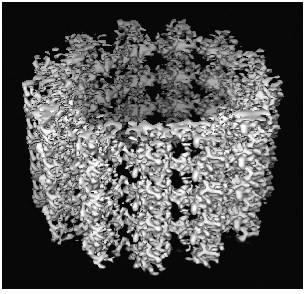
\includegraphics[width=.87\linewidth]{figures/ch09_fig04.pdf}
\caption{微小管の構造。約$8\,\text{\AA}$の分解能で得られた低温電子顕微鏡データに基づく、三次元再構成を示す。Lawrence Berkeley National LaboratoryのKen DowningのVisualization Groupが作成\cite{ref516,ref517}。}
\end{figure}
\begin{figure}[htbp]
\centering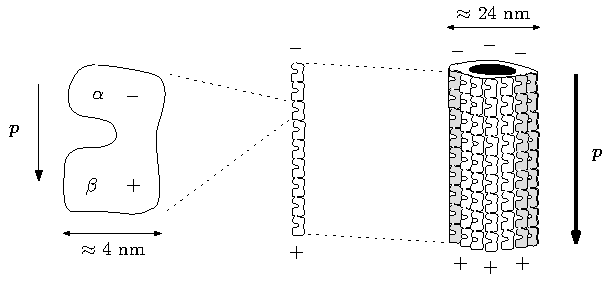
\includegraphics[width=.94\linewidth]{figures/ch09_fig05.pdf}
\caption{微小管の双極子モーメント。左：$\alpha$、$\beta$単量体からなる各チューブリン二量体は、小型の電気双極子として働く。中央：プロトフィラメントは、そのような電気双極子の鎖である。右：プロトフィラメントは、平行に束ねられて微小管を形成するため、微小管は個々のプロトフィラメントの双極子モーメントの和に等しい、双極子モーメントを持つ。}
\end{figure}

各二量体の内部には、非局在化した電子が一つ含まれ、それは、それぞれ$\alpha$サブユニット側と$\beta$サブユニット側にある、二つの疎水性ポケットのいずれかへ局在できる（図9.6）。
% 原文 p.373
\hypertarget{srcpage:373}{}\label{srcpage:373}
電子が$\beta$サブユニット側へ局在すると、二量体の$\beta$状態と呼ばれるが、二量体は、電子が$\alpha$サブユニット側に局在した立体配座、すなわち二量体の$\alpha$状態に対応する垂直軸から、約30度の立体配座変形を起こす。したがって、二量体は、立体配座状態$\alpha$と$\beta$に対応する基底状態を持つ、有効二状態系として記述できる。二量体が変形するため、電気双極子モーメントの向きは$\alpha$状態と$\beta$状態で異なり、これら二状態を、微小管軸方向の電気双極子モーメントの、二つの異なる値$p_\alpha$、$p_\beta$へ対応させられる。ゆえに、プロトフィラメントを、相互作用するIsingスピン$1/2$鎖の集合とみなせる。ここでは、スピンの「上」と「下」が、微小管軸方向の電気双極子モーメントの、二つの可能な状態$\alpha$と$\beta$に対応する。

\begin{figure}[htbp]
\centering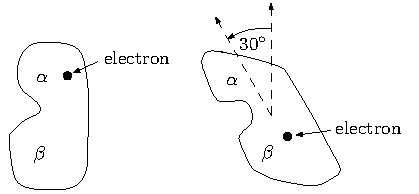
\includegraphics[width=.82\linewidth]{figures/ch09_fig06.pdf}
\caption{チューブリン二量体の二つの立体配座状態$\alpha$と$\beta$。}
\end{figure}

加水分解過程によるエネルギー供給のような、ある種の過程は、微小管の一端に位置するチューブリン二量体の、立体配座状態$\alpha$と$\beta$の間の変化を誘起できる\cite{ref518}。二量体間の双極子相互作用を介して、その二量体に付随する双極子モーメントの変化が、微小管軸に沿って高速に伝播する可能性が提案されている（図9.7参照）。Sataric、Tuszynski、Zakula\cite{ref519}は、微小管で損失なくエネルギーを輸送できる可能性を記述するため、そのような「キンク状」励起、すなわちソリトンの、詳しい理論模型を提案した。

\begin{figure}[htbp]
\centering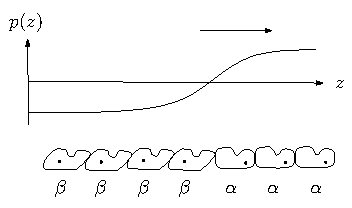
\includegraphics[width=.94\linewidth]{figures/ch09_fig07.pdf}
\caption{微小管中のキンク状励起の模型。微小管の一端で、チューブリン二量体の$\alpha$状態と$\beta$状態の間の立体配座転換に対応する、局所的双極子モーメントの変化が、二量体間の双極子相互作用を介して、微小管軸に沿って進む。これによって、微小管軸方向の双極子モーメント$p(z)$にキンク状励起が生じ、その励起が微小管軸に沿って高速で伝播する。簡単のため、ここでは$\alpha$状態と$\beta$状態を、微小管軸方向の電気双極子モーメントが、大きさは等しく向きが逆の値に対応させている。}
\end{figure}


% 原文 p.374
\hypertarget{srcpage:374}{}\label{srcpage:374}
Tegmark\cite{ref515}は、この特定の模型に焦点を当て、多数の二量体に相当する距離だけ離れた、二つのキンク状励起の重ね合わせについて、典型的なデコヒーレンス時間尺度を評価した。キンクの位置にある正味の電荷と、遠くの環境イオンとのCoulomb相互作用を考えた。その電荷は、微小管の断面をなす二量体の「輪」に含まれる、13個の$\beta$サブユニット中の、各18個の$\mathrm{Ca}^{2+}$イオンによる総電荷に等しいとした。十分離れた二つのキンクの重ね合わせのデコヒーレンス時間尺度$\tau_{\mathrm d}$は、遠くのイオンとの相互作用による、ニューロン重ね合わせのデコヒーレンスを模型化する際に使ったものと同様の、Coulomb散乱模型で評価された（9.3.1節参照）。Tegmarkは、$\tau_{\mathrm d}\approx10^{-13}\,\mathrm s$という値を得た（表9.1も参照）。微小管の量子コヒーレントな振る舞いの可能な本性を、この種の重ね合わせと同定するなら、Tegmarkの数値評価は、微小管が量子コンピューターのような量子コヒーレントな振る舞いを示す可能性を、かなり明瞭に排除する。

しかし、PenroseとHameroff\cite{ref473,ref512,ref513}が作った、かなり論争的な模型では、別の可能性が考えられている。ここでは、Tegmarkが調べた空間的に離れたキンク状励起の重ね合わせの代わりに、個々のチューブリン二量体の、二つの立体配座状態$\alpha$と$\beta$の重ね合わせを考える。微小管が量子コヒーレントな動力学を示すにはデコヒーレンスが強すぎる、というTegmarkの主張に異議を唱えるため、Hagan、Hameroff、Tuszynski\cite{ref514}は、個々の二量体を含むそのような配座の重ね合わせは、Tegmarkが評価したソリトンの重ね合わせのデコヒーレンス時間よりも、何桁も長いデコヒーレンス時間を可能にすると提案した。

$\alpha$状態と$\beta$状態の重ね合わせのデコヒーレンス時間を計算するため、Hagan、Hameroff、Tuszynski\cite{ref514}は、Tegmarkが使ったものと同様の模型を用いたが、それを単一二量体の双極子モーメントへ適用した。しかし、RosaとFaber\cite{ref520}が指摘したように、\cite{ref514}の計算における正当化できない近似を修正すると、得られるデコヒーレンス時間は、空間的に離れたキンク状励起の重ね合わせについて、Tegmarkがもともと与えた値と同程度になる。これらの評価は、Penrose--Hameroff型の模型を決定的に排除するものではないが、そのような理論に対する非常に重大な難題を提起する。

現在、大多数の研究者は、脳内の生物構造はおそらくデコヒーレンスを受けやす過ぎるため、認知過程や意識過程に関係する時間尺度にわたって、量子コヒーレンスを持続させることはできない、という見方を支持しているといってよい\cite{ref521}。したがって、脳の古典模型は、今日までほぼ揺るがされていない。Tegmarkの数値結果と、巨視的尺度でのデコヒーレンスについての一般的直観に基づけば、この状況が近い将来変わるとは考えにくい。


% 原文 p.375
\hypertarget{srcpage:375}{}\label{srcpage:375}
\subsectionlink{測定問題の「主観的」解決}
von Neumann連鎖の最終状態(9.1)は、観測者の異なる「心的状態」、すなわち$n$で区別される異なる結果の知覚に対応する状態が、装置、系などの相対状態と量子的に相関していることを記述する。そこで、測定問題の主観的解決を目指す方法は、全体の状態にコヒーレンスが存続しているにもかかわらず、可能な結果のうちただ一つだけを観測者が知覚することが、どのように生じ得るかを説明しようとする。この場合、「外部の物理的実在」が何であれ、それは全体の重ね合わせ状態(9.1)によって、完全に記述され続けてもよく、成分状態のどれか一つを選び出す経験的必要はない。9.1節で論じたように、理論が可能なすべての観測を正しく説明できるなら、このような測定問題の主観的解決を、満足のいく十分なものとみなすことを妨げる、根本的理由はない（\cite{ref001,ref322,ref496}も参照）。

上で述べたように、現在の科学的証拠は、すべてとはいわなくても大部分の認知活動、したがっておそらく観測者の「心の状態」ないし「心的状態」\footnote{以下の段落で引用符を頻繁に使うのは、「心」「意識」「心的状態」のような概念の、かなり曖昧な性格を、必然的に反映している。}が、脳内の神経回路網の特定の静止・発火パターンに結びつけられることを示唆する（知覚とニューロンパターンの関係について、より精密な定義は\cite{ref504,ref522}参照）。大まかにいえば、これは、(9.1)の右辺の抽象状態「観測者が結果$n$を知覚」のそれぞれが、ニューロンの集まりの特定の静止・発火パターンに対応することを意味する。上で見たように、発火状態と静止状態の重ね合わせは、環境との相互作用によって急速にデコヒーレンスする。したがって、このデコヒーレンスによって、添字$n$で区別される異なる結果に対応する、(9.1)右辺の「分枝」が、実用上不可逆に動力学的分離を起こすと結論するのは合理的である。

ここで、頑健なニューロンの指針状態、すなわち静止状態と発火状態が、私たちの周囲の世界の安定な準古典的指針状態と、なぜまさに量子的に相関するのか、すなわち(9.1)の「結果状態」が、なぜ私たちの経験するおなじみの状態に対応するのか、と問うことができる。たとえば、環境によって超選択されたニューロンの静止状態や発火状態は、巨視的に離れた状態の重ね合わせではなく、なぜ巨視的物体の空間的によく局在した状態と相関するのだろうか。利用できる相互作用Hamiltonianの集合が限られ、したがって検出可能な観測量の集合が強く制限される、という明白な理由に加えて、Zurek\cite{ref013}は、もう一つの重要な理由を指摘した。

% 原文 p.376
\hypertarget{srcpage:376}{}\label{srcpage:376}
\begin{quote}
私たちの感覚は、量子力学を検証する目的で進化したのではない。むしろ、適者生存が中心的役割を果たした過程で発達したのである。予測によって何も得られないなら、知覚に進化上の理由はない。そして、予測可能性のふるいが示すように、デコヒーレンスにもかかわらず頑健で、したがって実効的に古典的な量子状態だけが、予測可能な帰結を持つ。実際、古典的実在は、予測可能性とほとんど同義とみなすことができる。
\end{quote}
また、部分系間の客観的な物理相互作用によって定義される分枝が、異なる個々の測定結果についての主観的な意識経験に、本当に対応することを示す必要もある。すなわち、各分枝に結びついた、古典的なニューロンの静止・発火パターンが、異なる可能な結果の意識的知覚に対応する、脳内の関係する集団的記憶状態、すなわち「記録」状態を、実際に表すことを示すべきである。これは、前述したvon Neumannの「心身並行論」の原理\cite{ref060}に対応する。

いうまでもなく、量子力学自体から、主観的経験とその物理的対応物との関係を導くことはできない。この事実から、この結びつきという問いには、新しい物理法則の導入によってしか、完全には答えられないと結論する人々もいる\cite{ref504}。Zeh\cite{ref039,ref523}のような著者は、ニューロン過程において波動関数の成分がデコヒーレンスするという経験的事実が、量子力学の形式の中で「意識の存在」を仮定するための、決定的とまではいかなくても十分な根拠になると提案している。この描像では、動力学的に自律した意識ある観測者が、(9.1)型の全体の波動関数の頑健な成分に対応し、各成分は、確定した静止・発火パターンに対応する、デコヒーレンスしたニューロン状態で区別される。こうして、ユニタリーに発展する全体の量子状態ベクトルで記述される、単一の量子宇宙の中に、頑健な分枝によって定義される、多数の古典的「世界」が得られる。

この設定が与えられれば、観測者のそのような多数の意識的知覚が共に「存在」し得る一方、その共「存在」は明示的には決して経験的に確認できない、と結論することも、実際にはあながち無理ではない。このため、「存在する」「存在」という語を引用符に入れている。この観測不可能性を考慮し、Zehは、観測者の異なる意識的な版\footnote{観測者の同一性は、その観測者の特定の意識的知覚によって定まると考えられるため、この状況が、同じ観測者の異なる意識的な版を表すと論じるのは難しいかもしれない。}の「存在」を、「発見的な擬制」\cite{ref523}と呼んだ。異なる意識的知覚を表す多数の分枝の「存在」は、ユニタリー動力学の普遍的妥当性と、全体の量子状態の「実在論的」解釈を仮定することから、単に帰結するからである。


% 原文 p.377
\hypertarget{srcpage:377}{}\label{srcpage:377}
そこでの推測は、観測者の異なる意識的な版が互いを「意識」しないため、観測者の内側からの視点では、量子状態が何らかの形の物理的実在を記述し、ユニタリー動力学が普遍的に妥当するという仮定を捨てずに、経験的に要求される、確定した測定結果の知覚を説明できるはずだ、というものである。

驚くことではないが、こうして得られる量子力学の「多心」解釈（たとえば\cite{ref004,ref005,ref016,ref039,ref067,ref104,ref399,ref523}。8.2節も参照）を、多くの人は受け入れがたく感じる。その不快感を生むのは、このような見方の経験的適合性、すなわち実験的反証の可能性への懸念というより、別の点である。結局、デコヒーレンスに、ニューロンの静止・発火パターンと意識的知覚の出現との結びつきについての追加の仮定を組み合わせれば、観測者の水準で確定した結果の知覚を保証するには、実際に十分かもしれない。その追加の仮定は、それ自体、デコヒーレンス効果の中に物理的正当化を見いだすかもしれない。

むしろ、多心解釈、および「多世界」解釈（8.2節参照）に対する不快感は、それらが、私たちに深く根づいた哲学的直観、すなわち周囲の世界についての主観的観測は「客観的な外部の物理的実在」の、かなりよい鏡であるという直観に反する、という感覚に根ざしている。多心描像では、全体の量子状態で記述される量子宇宙は、世界の観測された構造とは、根本的に異なる形で「ある」ように見える。観測された構造は、観測者の局所性とデコヒーレンス過程によって定義される、単一の「古典的」分枝で与えられる。一方、この全体の量子宇宙の「存在」を、私たちはおそらく決して経験的に検証できないだろう。もちろん、これは最終的に、「他の」観測不可能な分枝の存在論的地位についての、純粋に哲学的な議論となる。結局、「物理的実在」「ある」といった用語が指し得るのは、主観的観測によって確認された、少なくとも確認可能な存在だけである。Zeh\cite{ref408}は、次のように述べている。
\begin{quote}
観測の後に、今や一つの成分だけが存在する、と必ずしも結論する必要はなく、一つの成分だけが観測される、とだけ結論すればよい。（中略）「同じ」観測者が異なる巨視的性質を記録することを記述する、重ね合わされた世界の成分は、動力学的に互いから完全に独立している。それらは異なる観測者を記述する。（中略）基本的な全体の配置空間上で、動力学的に分離する、すなわち「分枝する」波束の形で、Schrödinger方程式から導かれる、観測者の同一性の非決定性ないし分裂というこの結論を、受け入れがたい、あるいは「途方もない」と考える者は、代わりに、「他の」成分が消滅するという余分な仮説を、好みのどのような方法でも動力学的に形式化してよい。しかし、そのことで自分自身の問題を生むかもしれないと自覚すべきである。全体のSchrödinger方程式からのいかなるずれも、原理的には観測可能な効果を生じさせなければならず、そのような効果は、これまで一つも発見されていないことを思い出すべきである。
\end{quote}

% 原文 p.378
\hypertarget{srcpage:378}{}\label{srcpage:378}
個人の解釈上の好みにかかわらず、本節から持ち帰るべき主要な知見の一つは、デコヒーレンスが、多心的見方のような解釈の経験的適合性を保証する、核心的機構をなすということである（この問題は8.2節も参照）。実際、デコヒーレンスなしでは、多心解釈も多世界解釈も、成立する見込みがない。デコヒーレンス、より正確には、観測者を含む部分系間の物理的相互作用と、それによるもつれは、局所的な優先状態の出現を説明し、それによって分枝の構造を動力学的に定義する。また、デコヒーレンスは、これらの優先状態間の干渉効果が、局所観測者からは観測されないことを保証し、実効的に独立した、すなわち動力学的に分離された「古典的」分枝をもたらす。

とりわけニューロン状態の特定のパターンを含む、これらの分枝が、実際の意識経験と厳密にどう結びつくかという問いは、もちろん本質的に答えにくい。物理学、化学、生物学、心理学の多くの側面に関わるからである。しかし重要なのは、この現代的な「心身並行論」の実際的な詳細は、現時点で十分に理解されていない一方、デコヒーレンスが、観測者と観測を、純粋に量子力学的で経験的に適切な仕方で、原理的に記述するために必要な基本要素を与えることである。たとえば、デコヒーレンスによって「作られる」頑健で時間的に持続する分枝は、観測者に関係する本質的な性質をすべて含む。私たちが経験するおなじみの確定した量と相関し、環境にも冗長に刻み込まれる、明確に定まった安定な測定記録などである。収縮公準を外から導入したり、本質的に古典的な測定装置や、量子力学の法則外で収縮を誘起する意識の存在を仮定したりするのと対照的に、この記述は、普遍的に妥当する量子論に支配される、相互作用する物理系だけに基づいており、精密で定量的な理論的・実験的分析が可能である。


\clearpage
\setcounter{footnote}{0}
% 原文 p.379
\hypertarget{srcpage:379}{}\label{srcpage:379}
\sectionlink*{付録：相互作用描像}

演算子と量子状態を、いわゆる相互作用描像で表す手法は、量子力学的問題を摂動的に扱ううえで、非常に重要である。たとえば、4.2.2節で詳しく述べた、デコヒーレンスに対するBorn--Markovマスター方程式の導出で、重要な役割を果たす。以下で、相互作用描像による方法の基礎を復習しよう。

まず、次の形のHamiltonianを考える。
\begin{equation}
\hat H=\hat H_0+\hat V.\tag{A.1}
\end{equation}
ここで$\hat H_0$は、系Sの自由な、すなわち摂動されていない発展を記述するHamiltonianの部分であり、$\hat V$は、付け加えられた何らかの外部摂動である。相互作用描像の形式を応用するときには、通常、$\hat V$は$\hat H_0$に比べて弱いと仮定し、この仮定の下で系の近似的な動力学を決定することを目指す。しかし以下では、厳密な計算だけを行い、二成分$\hat H_0$と$\hat V$の相対的な強さについて、仮定を置かない。

標準量子論から、観測量演算子$\hat A(t)$の期待値は、トレース規則［(2.17)参照］によって与えられることが分かる。
\begin{equation}
\langle\hat A(t)\rangle=\operatorname{Tr}[\hat A(t)\hat\rho(t)]
=\operatorname{Tr}[\hat A(t)e^{-i\hat Ht}\hat\rho(0)e^{i\hat Ht}].\tag{A.2}
\end{equation}
すぐに明らかになる理由によって、この式を次のように書き換えよう。
\begin{equation}
\langle\hat A(t)\rangle=\operatorname{Tr}\left[\left(e^{i\hat H_0t}\hat A(t)e^{-i\hat H_0t}\right)
\left(e^{i\hat H_0t}e^{-i\hat Ht}\hat\rho(0)e^{i\hat Ht}e^{-i\hat H_0t}\right)\right].\tag{A.3}
\end{equation}
角括弧内の式の最初と最後へ、時間発展演算子$e^{\pm i\hat H_0t}$を挿入する際、トレースが引数の巡回置換に対して不変である、すなわち$\operatorname{Tr}(\hat A\hat B\hat C\cdots)=\operatorname{Tr}(\hat B\hat C\cdots\hat A)$などとなることを利用した。したがって、最初の因子$e^{i\hat H_0t}$をトレースの引数の最後へ動かすと、その位置の余分な因子$e^{-i\hat H_0t}$と相殺できる。

% 原文 p.380
\hypertarget{srcpage:380}{}\label{srcpage:380}
式(A.3)を動機として、一般の演算子$\hat A(t)$と密度行列$\hat\rho(t)$の、相互作用描像での形を導入する。
\begin{equation}
\hat A^{(\mathrm I)}(t)=e^{i\hat H_0t}\hat A(t)e^{-i\hat H_0t},\tag{A.4}
\end{equation}
\begin{equation}
\begin{aligned}
\hat\rho^{(\mathrm I)}(t)&=e^{i\hat H_0t}\hat\rho(t)e^{-i\hat H_0t}\\
&=e^{i\hat H_0t}e^{-i\hat Ht}\hat\rho(0)e^{i\hat Ht}e^{-i\hat H_0t}.
\end{aligned}\tag{A.5}
\end{equation}
ここでは上付き添字$(\mathrm I)$で、相互作用描像の演算子を表す。相互作用描像の演算子$\hat A^{(\mathrm I)}(t)$の動力学は、全Hamiltonian$\hat H$ではなく、摂動されていない自由なHamiltonian$\hat H_0$によって完全に定まることに注意しよう。

新しい定義(A.4)、(A.5)を用いると、期待値の式(A.3)は、簡潔な形に書ける。
\begin{equation}
\langle\hat A(t)\rangle=\operatorname{Tr}[\hat A^{(\mathrm I)}(t)\hat\rho^{(\mathrm I)}(t)].\tag{A.6}
\end{equation}
それでは、相互作用描像の密度行列$\hat\rho^{(\mathrm I)}(t)$の発展方程式を求めよう。Schrödinger描像の密度行列$\hat\rho(t)$について、標準的なLiouville--von Neumann方程式
\begin{equation}
\frac{\mathrm d}{\mathrm dt}\hat\rho(t)=-i[\hat H,\hat\rho(t)]\tag{A.7}
\end{equation}
を使うと、次を得る。
\begin{equation}
\begin{aligned}
\frac{\mathrm d}{\mathrm dt}\hat\rho^{(\mathrm I)}(t)
&=i[\hat H_0,\hat\rho^{(\mathrm I)}(t)]+e^{i\hat H_0t}\left(\frac{\mathrm d}{\mathrm dt}\hat\rho(t)\right)e^{-i\hat H_0t}\\
&\overset{\text{(A.7)}}=i[\hat H_0,\hat\rho^{(\mathrm I)}(t)]-ie^{i\hat H_0t}[\hat H,\hat\rho(t)]e^{-i\hat H_0t}\\
&\overset{\text{(A.1)}}=i[\hat H_0,\hat\rho^{(\mathrm I)}(t)]-ie^{i\hat H_0t}[\hat H_0+\hat V,\hat\rho(t)]e^{-i\hat H_0t}.
\end{aligned}\tag{A.8}
\end{equation}
(A.4)と(A.5)から、第二の交換子内の量に時間発展演算子$e^{\pm i\hat H_0t}$を適用することは、それらを相互作用描像へ変換することに相当すると分かる。したがって式(A.8)は、次のようになる。
\begin{equation}
\begin{aligned}
\frac{\mathrm d}{\mathrm dt}\hat\rho^{(\mathrm I)}(t)
&=i[\hat H_0,\hat\rho^{(\mathrm I)}(t)]-i[\hat H_0,\hat\rho^{(\mathrm I)}(t)]
-i[\hat V^{(\mathrm I)}(t),\hat\rho^{(\mathrm I)}(t)]\\
&=-i[\hat V^{(\mathrm I)}(t),\hat\rho^{(\mathrm I)}(t)].
\end{aligned}\tag{A.9}
\end{equation}
これで、第一の主要な結果が得られた。相互作用描像の密度演算子の時間発展は、Liouville--von Neumann型の方程式で与えられるが、全Hamiltonian$\hat H$の代わりに、相互作用描像の摂動$\hat V^{(\mathrm I)}(t)$が現れる。それにふさわしく、(A.9)は相互作用描像のLiouville--von Neumann方程式と呼ばれる。

% 原文 p.381
\hypertarget{srcpage:381}{}\label{srcpage:381}
ここまでは、起源をそれ以上指定しない何らかの摂動$\hat V$を受ける、単一の系Sを考えた。今度は、デコヒーレンスに関係する設定へ進もう。摂動は、相互作用Hamiltonian$\hat H_{\mathrm{int}}$で記述される、何らかの外部環境Eとの相互作用によるものとする。すなわち$\hat V\equiv\hat H_{\mathrm{int}}$である。系と環境の自己Hamiltonianを、それぞれ$\hat H_{\mathrm S}$、$\hat H_{\mathrm E}$と書けば、複合系SEの全Hamiltonianは、次の形に書ける。
\begin{equation}
\hat H=\hat H_0+\hat V\equiv\underbrace{\hat H_{\mathrm S}+\hat H_{\mathrm E}}_{\equiv\hat H_0}
+\underbrace{\hat H_{\mathrm{int}}}_{\equiv\hat V}.\tag{A.10}
\end{equation}
通常の方針に従い、縮約密度演算子$\hat\rho_{\mathrm S}(t)$の時間発展を決定したい。ここでは、相互作用描像の縮約密度演算子
\begin{equation}
\hat\rho_{\mathrm S}^{(\mathrm I)}(t)\equiv\operatorname{Tr}_{\mathrm E}[\hat\rho^{(\mathrm I)}(t)]\tag{A.11}
\end{equation}
を得たい。以下の二つの問いを扱う。
\begin{enumerate}
\item Schrödinger描像の縮約密度演算子$\hat\rho_{\mathrm S}(t)$が与えられたとき、対応する相互作用描像の演算子$\hat\rho_{\mathrm S}^{(\mathrm I)}(t)$は何か。
\item $\hat\rho_{\mathrm S}^{(\mathrm I)}(t)$に対する、適切な時間発展方程式は何か。
\end{enumerate}
第一の問いに答えよう。(A.11)のトレースを評価すると、次を得る。
\begin{equation}
\begin{aligned}
\operatorname{Tr}_{\mathrm E}[\hat\rho^{(\mathrm I)}(t)]
&\overset{\text{(A.5)}}=\operatorname{Tr}_{\mathrm E}[e^{i\hat H_0t}\hat\rho(t)e^{-i\hat H_0t}]\\
&\overset{\text{(A.10)}}=e^{i\hat H_{\mathrm S}t}\left\{\operatorname{Tr}_{\mathrm E}[e^{i\hat H_{\mathrm E}t}\hat\rho(t)e^{-i\hat H_{\mathrm E}t}]\right\}e^{-i\hat H_{\mathrm S}t}\\
&=e^{i\hat H_{\mathrm S}t}\{\operatorname{Tr}_{\mathrm E}[\hat\rho(t)]\}e^{-i\hat H_{\mathrm S}t}\\
&=e^{i\hat H_{\mathrm S}t}\hat\rho_{\mathrm S}(t)e^{-i\hat H_{\mathrm S}t}\\
&\overset{\text{(A.11)}}\equiv\hat\rho_{\mathrm S}^{(\mathrm I)}(t).
\end{aligned}\tag{A.12}
\end{equation}
ここで、最後から二番目の行では、引数の巡回置換に対するトレース操作の不変性を、再び使った。少し言い方を変えれば、引数のユニタリー変換に対するトレースの不変性である。

式(A.12)は、相互作用描像の縮約密度演算子が、Schrödinger描像の縮約密度演算子に、自由な系Hamiltonian$\hat H_{\mathrm S}$だけを含むユニタリー変換を施すことで得られることを示す。すなわち、
\begin{equation}
\hat\rho_{\mathrm S}^{(\mathrm I)}(t)=e^{i\hat H_{\mathrm S}t}\hat\rho_{\mathrm S}(t)e^{-i\hat H_{\mathrm S}t}.\tag{A.13}
\end{equation}
(A.13)と、相互作用描像の全密度演算子$\hat\rho^{(\mathrm I)}(t)$に対応する変換(A.5)の類似性は、これで明らかだろう。
% 原文 p.382
\hypertarget{srcpage:382}{}\label{srcpage:382}
いずれの場合にも、変換に含まれるのは自由Hamiltonianだけであり、$\hat\rho^{(\mathrm I)}(t)$に対しては$\hat H_0$、相互作用描像の縮約密度演算子$\hat\rho_{\mathrm S}^{(\mathrm I)}(t)$に対しては系Hamiltonian$\hat H_{\mathrm S}$である。

定義(A.13)はまた、望まれるように、系の観測量$\hat A_{\mathrm S}(t)$の期待値が、Schrödinger描像と相互作用描像で自動的に一致することを保証する。すなわち、
\begin{equation}
\langle\hat A_{\mathrm S}(t)\rangle=\operatorname{Tr}_{\mathrm S}[\hat\rho_{\mathrm S}(t)\hat A_{\mathrm S}(t)]
=\operatorname{Tr}_{\mathrm S}[\hat\rho_{\mathrm S}^{(\mathrm I)}(t)\hat A_{\mathrm S}^{(\mathrm I)}(t)],\tag{A.14}
\end{equation}
ここで、
\begin{equation}
\hat A_{\mathrm S}^{(\mathrm I)}(t)\overset{\text{(A.4)}}=e^{i\hat H_0t}\hat A_{\mathrm S}(t)e^{-i\hat H_0t}
\overset{\text{(A.10)}}=e^{i\hat H_{\mathrm S}t}\hat A_{\mathrm S}(t)e^{-i\hat H_{\mathrm S}t}.\tag{A.15}
\end{equation}
(A.14)の証明は直ちに得られる。
\begin{equation}
\begin{aligned}
\operatorname{Tr}_{\mathrm S}[\hat\rho_{\mathrm S}^{(\mathrm I)}(t)\hat A_{\mathrm S}^{(\mathrm I)}(t)]
&=\operatorname{Tr}_{\mathrm S}[e^{i\hat H_{\mathrm S}t}\hat\rho_{\mathrm S}(t)\hat A_{\mathrm S}(t)e^{-i\hat H_{\mathrm S}t}]\\
&=\operatorname{Tr}_{\mathrm S}[\hat\rho_{\mathrm S}(t)\hat A_{\mathrm S}(t)].
\end{aligned}\tag{A.16}
\end{equation}
最後に、先ほどの第二の問いに答え、相互作用描像の縮約密度演算子$\hat\rho_{\mathrm S}^{(\mathrm I)}(t)$の運動方程式を求めよう。相互作用描像の全密度演算子$\hat\rho^{(\mathrm I)}(t)$の発展方程式(A.9)で、$\hat V^{(\mathrm I)}(t)\equiv\hat H_{\mathrm{int}}^{(\mathrm I)}(t)$とし、両辺について環境のトレースを取ると、次を得る。
\begin{equation}
\frac{\mathrm d}{\mathrm dt}\hat\rho_{\mathrm S}^{(\mathrm I)}(t)
=-i\operatorname{Tr}_{\mathrm E}[\hat H_{\mathrm{int}}^{(\mathrm I)}(t),\hat\rho^{(\mathrm I)}(t)].\tag{A.17}
\end{equation}
よく見ると、この方程式は標準的なLiouville--von Neumannの形ではない。右辺が、縮約密度演算子$\hat\rho_{\mathrm S}^{(\mathrm I)}(t)$ではなく、全密度演算子$\hat\rho^{(\mathrm I)}(t)$に依存するからである。この事実は、読者にとってそれほど意外ではないだろう。結局、環境の状態は一般に、縮約密度演算子の発展に影響するのである。

したがって一般には、縮約動力学を決めるために、相互作用する系と環境の組全体を考えなければならない。この点は、もちろん、Schrödinger描像と相互作用描像のどちらで考えるかとは無関係である。系と環境の結合が弱いといった、ある近似を課して初めて、時間依存する全体の系・環境密度演算子に明示的には依存しない、系の縮約密度演算子の発展方程式が得られる。そのようなマスター方程式は、第4章と第5章で導かれる。


\clearpage
\renewcommand{\refname}{\hyperlink{toc}{参考文献}}
\bibliographystyle{utphys}
\bibliography{ref}
\clearpage
\sectionlink*{索引}
\begingroup\small
\setlength{\parindent}{0pt}
\setlength{\parskip}{1pt}
\newcommand{\idxentry}[2]{\par\noindent\hangindent=1em\hangafter=1\textbf{#1}\quad#2\par}
\newcommand{\idxsub}[2]{\par\noindent\hangindent=2em\hangafter=1\hspace*{1em}#1\quad#2\par}
\begin{multicols}{2}
\raggedcolumns
\idxentry{観測による現実化}{\sourcepageref{19}}
\idxentry{補助系（アンシラ）}{\sourcepageref{311}--\sourcepageref{320}}
\idxentry{異常拡散係数}{\sourcepageref{186}, \sourcepageref{191}, \sourcepageref{200}, \sourcepageref{205}, \sourcepageref{220}}
\idxentry{装置}{\sourcepageref{32}, \sourcepageref{49}, \sourcepageref{51}, \sourcepageref{320}--\sourcepageref{321}}
\idxentry{人工神経回路網}{\sourcepageref{365}}
\idxentry{非対称エネルギー}{\sourcepageref{174}}
\idxentry{軸索}{\sourcepageref{368}}
\idxentry{浴}{\sourcepageref{171}}
\idxentry{ビアブル（beables）}{\sourcepageref{16}}
\idxentry{Bell不等式}{\sourcepageref{17}}
\idxentry{Bell状態}{\sourcepageref{29}, \sourcepageref{32}}
\idxentry{双線形結合}{\sourcepageref{179}}
\idxentry{ビット反転誤り}{\sourcepageref{309}}
\idxentry{測定のブラックボックス的見方}{\sourcepageref{334}}
\idxentry{Bloch球}{\sourcepageref{295}}
\idxentry{Bohm力学}{\sourcepageref{18}, \sourcepageref{354}--\sourcepageref{357}}
\idxsub{デコヒーレンスとの関係}{\sourcepageref{356}--\sourcepageref{357}}
\idxsub{粒子概念}{\sourcepageref{356}}
\idxsub{軌道}{\sourcepageref{355}}
\idxentry{Born近似}{\sourcepageref{156}, \sourcepageref{160}--\sourcepageref{161}}
\idxentry{Born確率}{\sourcepageref{35}, \sourcepageref{333}}
\idxentry{Born則}{\sourcepageref{15}, \sourcepageref{35}, \sourcepageref{331}}
\idxsub{エンバリアンスとの関係}{\sourcepageref{341}--\sourcepageref{343}}
\idxsub{Zurekによる導出}{\sourcepageref{341}--\sourcepageref{343}}
\idxentry{Born–Markovマスター方程式}{\sourcepageref{155}--\sourcepageref{165}}
\idxsub{導入される仮定}{\sourcepageref{156}}
\idxsub{導出}{\sourcepageref{158}--\sourcepageref{165}}
\idxsub{構造}{\sourcepageref{156}--\sourcepageref{158}}
\idxentry{Born–Pauli解釈}{\sourcepageref{19}}
\idxentry{Bose–Einstein凝縮体}{\sourcepageref{282}--\sourcepageref{283}}
\idxentry{脳}{\sourcepageref{359}--\sourcepageref{378}}
\idxentry{分枝}{\sourcepageref{337}, \sourcepageref{375}}
\idxentry{$\mathrm C_{70}$の干渉実験}{\sourcepageref{258}--\sourcepageref{270}}
\idxsub{熱放射の放出}{\sourcepageref{265}--\sourcepageref{267}}
\idxsub{干渉模様}{\sourcepageref{262}--\sourcepageref{263}}
\idxsub{実験配置}{\sourcepageref{259}--\sourcepageref{262}}
\idxsub{経路情報}{\sourcepageref{263}--\sourcepageref{265}}
\idxentry{Caldeira–Leggettマスター方程式}{\sourcepageref{191}--\sourcepageref{194}}
\idxentry{標準模型}{\sourcepageref{171}--\sourcepageref{241}}
\idxentry{共振器量子電気力学}{\sourcepageref{255}}
\idxentry{電荷量子ビット}{\sourcepageref{281}}
\idxentry{キラル分子}{\sourcepageref{83}}
\idxentry{古典的集団}{\sourcepageref{37}}
\idxentry{CNOTゲート}{\sourcepageref{306}}
\idxentry{粗視化}{\sourcepageref{37}, \sourcepageref{59}}
\idxentry{符号部分空間}{\sourcepageref{315}}
\idxentry{コヒーレンス}{\sourcepageref{5}, \sourcepageref{20}}
\idxsub{非局在化}{\sourcepageref{8}}
\idxsub{再帰}{\sourcepageref{92}, \sourcepageref{213}}
\idxsub{再局在化}{\sourcepageref{99}, \sourcepageref{255}--\sourcepageref{258}}
\idxsub{復活}{\sourcepageref{98}--\sourcepageref{101}, \sourcepageref{255}--\sourcepageref{258}}
\idxentry{コヒーレンス長}{\sourcepageref{140}--\sourcepageref{147}}
\idxentry{コヒーレント振動}{\sourcepageref{275}--\sourcepageref{279}}
\idxentry{コヒーレントな広がり}{\sourcepageref{116}, \sourcepageref{144}, \sourcepageref{145}}
\idxentry{コヒーレント状態}{\sourcepageref{117}, \sourcepageref{202}, \sourcepageref{249}}
\idxentry{収縮公準}{\sourcepageref{3}, \sourcepageref{15}, \sourcepageref{331}}
\idxentry{可換性基準}{\sourcepageref{77}}
\idxentry{相補性原理}{\sourcepageref{61}--\sourcepageref{65}}
\idxentry{条件付き量子動力学}{\sourcepageref{306}}
\idxentry{共役基底}{\sourcepageref{23}}
\idxentry{意識}{\sourcepageref{363}--\sourcepageref{367}, \sourcepageref{370}--\sourcepageref{371}, \sourcepageref{376}--\sourcepageref{378}}
\idxentry{保存則}{\sourcepageref{30}}
\idxentry{文脈依存性}{\sourcepageref{18}}
\idxentry{連続的自発的局在化}{\sourcepageref{349}--\sourcepageref{354}}
\idxentry{量子コンピューターにおける制御可能性}{\sourcepageref{301}--\sourcepageref{302}}
\idxentry{Cooper対}{\sourcepageref{271}}
\idxentry{Copenhagen解釈}{\sourcepageref{330}--\sourcepageref{336}, \sourcepageref{360}, \sourcepageref{363}}
\idxentry{相関}{}
\idxsub{古典的}{\sourcepageref{30}}
\idxsub{量子的}{\sourcepageref{29}}
\idxsub{量子的相関と古典的相関}{\sourcepageref{30}--\sourcepageref{32}}
\idxentry{dc-SQUID}{\sourcepageref{272}}
\idxentry{de Broglie波長（物質）}{\sourcepageref{116}}
\idxentry{de Broglie波長（熱的）}{\sourcepageref{94}}
\idxentry{デコヒーレンス}{}
\idxsub{量子誤り訂正との関係}{\sourcepageref{311}--\sourcepageref{321}}
\idxsub{部分系への分割との関係}{\sourcepageref{101}--\sourcepageref{103}}
\idxsub{装置が誘起するもの}{\sourcepageref{320}--\sourcepageref{321}}
\idxsub{標準模型}{\sourcepageref{171}--\sourcepageref{241}}
\idxsub{集団的}{\sourcepageref{322}--\sourcepageref{323}}
\idxsub{環境散乱によるもの}{\sourcepageref{115}--\sourcepageref{151}}
\idxsub{散乱誘起デコヒーレンスの動力学}{\sourcepageref{139}--\sourcepageref{150}}
\idxsub{実験}{\sourcepageref{243}--\sourcepageref{291}}
\idxsub{因子}{\sourcepageref{91}, \sourcepageref{122}, \sourcepageref{212}}
\idxsub{偽のもの}{\sourcepageref{96}}
\idxsub{歴史}{\sourcepageref{10}--\sourcepageref{12}}
\idxsub{Bose–Einstein凝縮体におけるもの}{\sourcepageref{282}--\sourcepageref{283}}
\idxsub{共振器QEDにおけるもの}{\sourcepageref{251}--\sourcepageref{258}}
\idxsub{エネルギーでのもの}{\sourcepageref{81}, \sourcepageref{228}}
\idxsub{量子力学の解釈におけるもの}{\sourcepageref{329}--\sourcepageref{358}}
\idxsub{運動量でのもの}{\sourcepageref{194}}
\idxsub{ニューロンにおけるもの}{\sourcepageref{368}--\sourcepageref{371}}
\idxsub{位相空間でのもの}{\sourcepageref{173}, \sourcepageref{194}--\sourcepageref{203}}
\idxsub{量子Brown運動におけるもの}{\sourcepageref{178}--\sourcepageref{206}}
\idxsub{量子コンピューターにおけるもの}{\sourcepageref{293}--\sourcepageref{328}}
\idxsub{量子電気機械系におけるもの}{\sourcepageref{287}--\sourcepageref{288}}
\idxsub{SQUIDにおけるもの}{\sourcepageref{279}--\sourcepageref{282}}
\idxsub{脳におけるもの}{\sourcepageref{365}--\sourcepageref{374}}
\idxsub{独立なもの}{\sourcepageref{322}--\sourcepageref{323}}
\idxsub{不可逆性}{\sourcepageref{5}, \sourcepageref{69}}
\idxsub{動力学的時間尺度でのもの}{\sourcepageref{197}}
\idxsub{率}{$\to$ デコヒーレンス率}
\idxsub{逆転}{\sourcepageref{98}--\sourcepageref{101}, \sourcepageref{255}--\sourcepageref{258}}
\idxsub{時間尺度（一般）}{\sourcepageref{94}}
\idxsub{時間尺度（量子Brown運動）}{\sourcepageref{197}}
\idxsub{時間尺度（散乱）}{\sourcepageref{127}, \sourcepageref{131}, \sourcepageref{134}}
\idxsub{仮想的}{\sourcepageref{98}--\sourcepageref{101}}
\idxsub{古典的雑音との比較}{\sourcepageref{95}--\sourcepageref{98}, \sourcepageref{302}--\sourcepageref{304}}
\idxsub{制御可能性との比較}{\sourcepageref{301}--\sourcepageref{302}}
\idxsub{散逸との比較}{\sourcepageref{93}--\sourcepageref{95}}
\idxentry{デコヒーレンス率}{\sourcepageref{70}, \sourcepageref{94}}
\idxsub{環境散乱におけるもの}{\sourcepageref{131}, \sourcepageref{134}}
\idxsub{微小管におけるもの}{\sourcepageref{371}--\sourcepageref{374}}
\idxsub{ニューロンにおけるもの}{\sourcepageref{368}--\sourcepageref{371}}
\idxsub{Caldeira–Leggett模型におけるもの}{\sourcepageref{193}}
\idxsub{スピン・ボソン模型におけるもの}{\sourcepageref{216}}
\idxsub{飽和}{\sourcepageref{132}, \sourcepageref{203}}
\idxentry{デコヒーレンス時間尺度}{$\to$ デコヒーレンス率}
\idxentry{デコヒーレンスのない部分空間}{\sourcepageref{79}--\sourcepageref{80}, \sourcepageref{321}--\sourcepageref{327}}
\idxsub{実験的実現}{\sourcepageref{325}--\sourcepageref{326}}
\idxsub{構造と大きさ}{\sourcepageref{322}--\sourcepageref{325}}
\idxentry{遅延選択実験}{\sourcepageref{100}}
\idxentry{位相関係の非局在化}{\sourcepageref{69}, \sourcepageref{98}--\sourcepageref{101}}
\idxentry{非局在モード}{\sourcepageref{175}}
\idxentry{密度行列}{\sourcepageref{33}--\sourcepageref{49}}
\idxsub{基底の曖昧さ}{\sourcepageref{41}--\sourcepageref{42}}
\idxsub{解釈}{\sourcepageref{36}, \sourcepageref{39}, \sourcepageref{48}--\sourcepageref{49}}
\idxsub{混合状態のもの}{\sourcepageref{36}--\sourcepageref{41}}
\idxsub{純粋状態のもの}{\sourcepageref{34}--\sourcepageref{36}}
\idxsub{純粋度}{\sourcepageref{40}}
\idxsub{縮約されたもの}{\sourcepageref{44}--\sourcepageref{49}}
\idxsub{von Neumannエントロピー}{\sourcepageref{41}}
\idxentry{密度演算子}{$\to$ 密度行列}
\idxentry{位相緩和}{\sourcepageref{97}, \sourcepageref{270}, \sourcepageref{282}}
\idxentry{微分断面積}{\sourcepageref{123}}
\idxentry{直接ピーク}{\sourcepageref{107}}
\idxentry{散逸}{\sourcepageref{93}--\sourcepageref{95}, \sourcepageref{188}--\sourcepageref{191}}
\idxentry{散逸核}{\sourcepageref{181}}
\idxentry{識別可能性}{\sourcepageref{32}--\sourcepageref{33}, \sourcepageref{47}--\sourcepageref{48}}
\idxentry{二重スリット実験}{\sourcepageref{23}, \sourcepageref{60}, \sourcepageref{258}--\sourcepageref{259}, \sourcepageref{355}}
\idxentry{二重井戸ポテンシャル}{\sourcepageref{174}, \sourcepageref{273}}
\idxentry{動力学的分離}{\sourcepageref{10}, \sourcepageref{326}--\sourcepageref{327}, \sourcepageref{375}}
\idxentry{動力学的対称性}{\sourcepageref{80}}
\idxentry{動力学的に分離された部分空間}{\sourcepageref{327}}
\idxentry{Dyson級数}{\sourcepageref{210}}
\idxentry{固有値・固有状態リンク}{\sourcepageref{59}, \sourcepageref{331}}
\idxentry{アインセレクション}{$\to$ 環境誘起超選択}
\idxentry{熱放射の放出}{\sourcepageref{115}, \sourcepageref{265}--\sourcepageref{267}}
\idxentry{集団}{}
\idxsub{平均}{\sourcepageref{43}, \sourcepageref{96}}
\idxsub{古典的（真正）}{\sourcepageref{20}}
\idxsub{位相緩和}{\sourcepageref{97}, \sourcepageref{270}, \sourcepageref{282}}
\idxsub{非真正}{\sourcepageref{49}}
\idxsub{集団解釈}{\sourcepageref{19}}
\idxsub{物理的}{\sourcepageref{43}--\sourcepageref{44}, \sourcepageref{96}, \sourcepageref{303}}
\idxsub{幅}{\sourcepageref{141}--\sourcepageref{147}}
\idxentry{もつれ}{\sourcepageref{4}, \sourcepageref{28}--\sourcepageref{33}}
\idxsub{識別可能性との関係}{\sourcepageref{32}--\sourcepageref{33}}
\idxsub{経路情報との関係}{\sourcepageref{60}--\sourcepageref{68}}
\idxsub{資源として}{\sourcepageref{7}}
\idxsub{定量化}{\sourcepageref{32}--\sourcepageref{33}}
\idxentry{エントロピー}{\sourcepageref{41}, \sourcepageref{313}}
\idxsub{Shannon}{\sourcepageref{86}}
\idxsub{熱力学的}{\sourcepageref{41}}
\idxsub{von Neumann}{\sourcepageref{41}}
\idxentry{エンバリアンス}{\sourcepageref{341}--\sourcepageref{343}}
\idxentry{証人としての環境}{\sourcepageref{86}}
\idxentry{環境設計}{\sourcepageref{326}--\sourcepageref{327}}
\idxentry{環境自己相関関数}{\sourcepageref{157}, \sourcepageref{181}}
\idxentry{環境援助不変性}{\sourcepageref{341}--\sourcepageref{343}}
\idxentry{環境誘起超選択}{\sourcepageref{6}, \sourcepageref{71}--\sourcepageref{85}}
\idxsub{解釈に対する含意}{\sourcepageref{329}--\sourcepageref{358}}
\idxsub{予測可能性のふるいとの関係}{\sourcepageref{82}--\sourcepageref{83}}
\idxsub{可換性基準}{\sourcepageref{77}}
\idxsub{一般の場合}{\sourcepageref{81}--\sourcepageref{83}}
\idxsub{Bohm力学におけるもの}{\sourcepageref{356}--\sourcepageref{357}}
\idxsub{様相解釈におけるもの}{\sourcepageref{345}--\sourcepageref{346}}
\idxsub{物理的収縮理論におけるもの}{\sourcepageref{349}--\sourcepageref{351}}
\idxsub{相対状態解釈におけるもの}{\sourcepageref{337}--\sourcepageref{344}}
\idxsub{Copenhagen解釈におけるもの}{\sourcepageref{334}--\sourcepageref{335}}
\idxsub{デコヒーレンスの量子極限におけるもの}{\sourcepageref{81}}
\idxsub{量子測定極限におけるもの}{\sourcepageref{76}--\sourcepageref{80}}
\idxsub{電荷のもの}{\sourcepageref{84}}
\idxsub{位置のもの}{\sourcepageref{83}}
\idxsub{安定性基準}{\sourcepageref{73}}
\idxentry{環境による監視}{\sourcepageref{65}--\sourcepageref{68}, \sourcepageref{78}}
\idxentry{環境散乱}{\sourcepageref{65}, \sourcepageref{115}--\sourcepageref{151}}
\idxentry{環境の自己相関}{\sourcepageref{156}, \sourcepageref{163}}
\idxentry{認識論的見方}{\sourcepageref{19}}
\idxentry{EPR}{\sourcepageref{6}, \sourcepageref{31}}
\idxentry{実存的解釈}{\sourcepageref{344}}
\idxentry{忠実な測定}{\sourcepageref{75}}
\idxentry{偽のデコヒーレンス}{\sourcepageref{96}}
\idxentry{耐故障性}{\sourcepageref{320}--\sourcepageref{321}}
\idxentry{第一の介入}{\sourcepageref{58}, \sourcepageref{363}}
\idxentry{磁束量子}{\sourcepageref{272}}
\idxentry{Fokker–Planck方程式}{\sourcepageref{184}}
\idxentry{自由意志}{\sourcepageref{366}}
\idxentry{ゲート操作}{\sourcepageref{296}}
\idxentry{Gauss型密度行列}{\sourcepageref{140}}
\idxentry{Gauss波束}{\sourcepageref{116}}
\idxentry{Groverの探索アルゴリズム}{\sourcepageref{300}}
\idxentry{GRW理論}{$\to$ 物理的収縮理論}
\idxentry{誘導方程式}{\sourcepageref{355}}
\idxentry{Hadamard回転}{\sourcepageref{317}}
\idxentry{Hamiltonian}{}
\idxsub{相互作用}{\sourcepageref{76}}
\idxsub{Lambシフトを含むもの}{\sourcepageref{155}}
\idxsub{開放系への分解}{\sourcepageref{76}}
\idxsub{自己Hamiltonian}{\sourcepageref{76}}
\idxentry{調和振動子}{\sourcepageref{117}, \sourcepageref{171}}
\idxentry{Heisenberg切断}{\sourcepageref{27}, \sourcepageref{335}}
\idxentry{発見的な擬制}{\sourcepageref{376}}
\idxentry{隠れた変数理論}{\sourcepageref{17}--\sourcepageref{18}, \sourcepageref{355}}
\idxentry{Hilbert空間}{\sourcepageref{15}}
\idxentry{Hyperion}{\sourcepageref{118}}
\idxentry{理想的量子測定}{\sourcepageref{52}}
\idxentry{無知で解釈できる混合}{\sourcepageref{42}}
\idxentry{非真正混合}{\sourcepageref{49}, \sourcepageref{69}, \sourcepageref{333}}
\idxentry{無限後退}{\sourcepageref{362}}
\idxentry{情報は物理的である}{\sourcepageref{294}, \sourcepageref{344}}
\idxentry{相互作用Hamiltonian}{\sourcepageref{76}}
\idxsub{対角分解}{\sourcepageref{78}}
\idxentry{相互作用描像}{\sourcepageref{379}--\sourcepageref{382}}
\idxentry{相互作用描像のLiouville–von Neumann方程式}{\sourcepageref{380}}
\idxentry{干渉}{\sourcepageref{47}--\sourcepageref{48}}
\idxsub{識別可能性との関係}{\sourcepageref{47}--\sourcepageref{48}}
\idxsub{実験}{\sourcepageref{23}--\sourcepageref{26}, \sourcepageref{243}--\sourcepageref{291}}
\idxsub{Bose–Einstein凝縮体におけるもの}{\sourcepageref{282}--\sourcepageref{283}}
\idxsub{$\mathrm C_{70}$回折におけるもの}{\sourcepageref{258}--\sourcepageref{270}}
\idxsub{SQUIDにおけるもの}{\sourcepageref{275}--\sourcepageref{279}}
\idxsub{局所的抑制}{\sourcepageref{68}--\sourcepageref{71}}
\idxsub{観測不可能性}{\sourcepageref{50}, \sourcepageref{55}--\sourcepageref{57}, \sourcepageref{333}}
\idxsub{模様}{\sourcepageref{23}, \sourcepageref{24}, \sourcepageref{55}, \sourcepageref{60}}
\idxsub{項}{\sourcepageref{34}}
\idxentry{内部環境}{\sourcepageref{176}}
\idxentry{解釈基底}{\sourcepageref{339}}
\idxentry{イオントラップ}{\sourcepageref{301}, \sourcepageref{303}, \sourcepageref{305}, \sourcepageref{326}}
\idxentry{不可逆性}{}
\idxsub{情報喪失との関係}{\sourcepageref{101}}
\idxsub{量子消去との関係}{\sourcepageref{100}}
\idxsub{収縮のもの}{\sourcepageref{63}}
\idxsub{デコヒーレンスのもの}{\sourcepageref{69}, \sourcepageref{93}, \sourcepageref{98}, \sourcepageref{304}}
\idxsub{測定のもの}{\sourcepageref{69}, \sourcepageref{100}}
\idxentry{孤立系}{\sourcepageref{1}--\sourcepageref{8}}
\idxentry{Itô方程式}{\sourcepageref{349}}
\idxentry{Josephson効果}{\sourcepageref{271}}
\idxentry{Josephson接合}{\sourcepageref{272}}
\idxentry{微小管中のキンク状励起}{\sourcepageref{374}}
\idxentry{Kochen–Specker定理}{\sourcepageref{18}}
\idxentry{Kraus演算子形式}{\sourcepageref{110}--\sourcepageref{112}}
\idxentry{Lambシフトを含むHamiltonian}{\sourcepageref{155}}
\idxentry{Lindbladマスター方程式}{\sourcepageref{165}--\sourcepageref{169}}
\idxentry{Lindblad演算子}{\sourcepageref{167}}
\idxentry{Liouville–von Neumann方程式}{\sourcepageref{139}}
\idxsub{相互作用描像}{\sourcepageref{380}}
\idxentry{局所理論}{\sourcepageref{4}}
\idxentry{状態の局所性}{\sourcepageref{4}}
\idxentry{局在化}{\sourcepageref{115}--\sourcepageref{151}}
\idxentry{局在モード}{\sourcepageref{175}}
\idxentry{長波長極限}{}
\idxsub{環境散乱におけるもの}{\sourcepageref{130}--\sourcepageref{132}}
\idxsub{量子Brown運動におけるもの}{\sourcepageref{204}}
\idxentry{Loschmidtエコー}{\sourcepageref{88}}
\idxentry{低温環境}{\sourcepageref{175}}
\idxentry{多心解釈}{\sourcepageref{337}, \sourcepageref{377}}
\idxentry{多世界解釈}{\sourcepageref{337}}
\idxentry{写像}{\sourcepageref{173}--\sourcepageref{178}}
\idxsub{振動子環境とスピン環境との関係}{\sourcepageref{176}--\sourcepageref{178}}
\idxsub{中心系のもの}{\sourcepageref{173}--\sourcepageref{174}}
\idxsub{振動子環境のもの}{\sourcepageref{175}}
\idxsub{位相空間粒子のもの}{\sourcepageref{173}}
\idxsub{スピン環境のもの}{\sourcepageref{175}--\sourcepageref{176}}
\idxsub{スピン環境から振動子環境へのもの}{\sourcepageref{228}--\sourcepageref{237}}
\idxsub{二準位系のもの}{\sourcepageref{173}--\sourcepageref{174}}
\idxentry{Markov近似}{\sourcepageref{156}, \sourcepageref{163}}
\idxentry{マスター方程式}{\sourcepageref{153}--\sourcepageref{170}}
\idxsub{Born–Markov形}{\sourcepageref{155}--\sourcepageref{165}}
\idxsub{一般形式}{\sourcepageref{154}--\sourcepageref{155}}
\idxsub{Caldeira–Leggett形}{\sourcepageref{191}--\sourcepageref{194}}
\idxsub{Lindblad形}{\sourcepageref{165}--\sourcepageref{169}}
\idxsub{非Markov型}{\sourcepageref{169}--\sourcepageref{170}}
\idxentry{測定問題}{\sourcepageref{49}--\sourcepageref{60}}
\idxsub{主観的解決}{\sourcepageref{375}--\sourcepageref{378}}
\idxentry{測定型相互作用}{\sourcepageref{49}, \sourcepageref{67}}
\idxentry{測定}{\sourcepageref{15}}
\idxsub{現実化}{\sourcepageref{19}}
\idxsub{事後選択との関係}{\sourcepageref{21}}
\idxsub{Born–Pauli解釈}{\sourcepageref{19}}
\idxsub{収縮}{\sourcepageref{15}}
\idxsub{文脈依存性}{\sourcepageref{18}}
\idxsub{干渉}{\sourcepageref{21}--\sourcepageref{26}}
\idxsub{不可逆なもの}{\sourcepageref{69}, \sourcepageref{100}}
\idxsub{局所的なもの}{\sourcepageref{44}}
\idxsub{非可換性}{\sourcepageref{15}}
\idxsub{非破壊}{\sourcepageref{52}, \sourcepageref{74}}
\idxsub{観測量との関係}{\sourcepageref{15}}
\idxsub{重ね合わせのもの}{\sourcepageref{21}--\sourcepageref{26}}
\idxsub{射影的なもの}{\sourcepageref{15}}
\idxsub{仮想的なもの}{\sourcepageref{101}}
\idxentry{記憶効果}{\sourcepageref{156}, \sourcepageref{163}, \sourcepageref{169}}
\idxentry{微小管}{\sourcepageref{367}, \sourcepageref{371}--\sourcepageref{374}}
\idxentry{混合状態}{\sourcepageref{19}, \sourcepageref{36}--\sourcepageref{41}}
\idxentry{混合}{}
\idxsub{無知で解釈できるもの}{\sourcepageref{42}}
\idxsub{非真正}{\sourcepageref{49}, \sourcepageref{69}, \sourcepageref{333}}
\idxsub{真正}{\sourcepageref{20}, \sourcepageref{42}}
\idxentry{様相解釈}{\sourcepageref{344}--\sourcepageref{347}}
\idxsub{環境誘起超選択との関係}{\sourcepageref{345}--\sourcepageref{346}}
\idxsub{Schmidt分解}{\sourcepageref{346}--\sourcepageref{347}}
\idxentry{模型}{}
\idxsub{標準的}{\sourcepageref{171}--\sourcepageref{241}}
\idxsub{量子Brown運動のもの}{\sourcepageref{178}--\sourcepageref{206}}
\idxsub{スピン・ボソン}{\sourcepageref{207}--\sourcepageref{222}}
\idxsub{スピン環境}{\sourcepageref{88}--\sourcepageref{93}, \sourcepageref{222}--\sourcepageref{237}}
\idxentry{相互情報量}{\sourcepageref{86}}
\idxentry{ミエリン}{\sourcepageref{368}}
\idxentry{ニューロン}{\sourcepageref{365}--\sourcepageref{371}, \sourcepageref{375}--\sourcepageref{378}}
\idxentry{NMR}{\sourcepageref{88}, \sourcepageref{97}, \sourcepageref{301}}
\idxentry{複製不可能定理}{\sourcepageref{16}, \sourcepageref{306}}
\idxentry{信号伝達不能定理}{\sourcepageref{31}}
\idxentry{雑音核}{\sourcepageref{181}}
\idxentry{非Hermite観測量}{\sourcepageref{53}}
\idxentry{非Markov動力学}{\sourcepageref{169}--\sourcepageref{170}}
\idxentry{観測量の非可換性}{\sourcepageref{15}, \sourcepageref{54}}
\idxentry{非破壊測定}{\sourcepageref{52}}
\idxsub{環境によるもの}{\sourcepageref{74}}
\idxentry{非局所性}{\sourcepageref{4}, \sourcepageref{6}, \sourcepageref{32}}
\idxentry{非ユニタリー動力学}{\sourcepageref{10}, \sourcepageref{28}, \sourcepageref{69}, \sourcepageref{111}, \sourcepageref{155}, \sourcepageref{290}, \sourcepageref{331}, \sourcepageref{348}--\sourcepageref{354}}
\idxentry{通常拡散係数}{\sourcepageref{185}, \sourcepageref{189}, \sourcepageref{191}, \sourcepageref{200}}
\idxentry{核磁気共鳴}{\sourcepageref{88}, \sourcepageref{97}, \sourcepageref{301}}
\idxentry{冗長性による客観化}{\sourcepageref{88}}
\idxentry{観測量}{\sourcepageref{15}}
\idxentry{観測}{}
\idxsub{量子力学におけるもの}{\sourcepageref{359}--\sourcepageref{361}}
\idxsub{間接的なもの}{\sourcepageref{85}}
\idxentry{非対角項}{\sourcepageref{34}}
\idxentry{量子系の開放性}{\sourcepageref{3}--\sourcepageref{4}, \sourcepageref{69}, \sourcepageref{74}}
\idxentry{演算子和形式}{\sourcepageref{110}--\sourcepageref{112}}
\idxentry{光量子計算}{\sourcepageref{301}}
\idxentry{正統的解釈}{\sourcepageref{330}--\sourcepageref{336}}
\idxentry{振動子環境}{\sourcepageref{175}}
\idxsub{弱結合極限}{\sourcepageref{176}}
\idxentry{結果}{\sourcepageref{16}}
\idxsub{隠れた変数理論におけるもの}{\sourcepageref{17}}
\idxsub{結果の問題}{\sourcepageref{50}, \sourcepageref{57}--\sourcepageref{60}, \sourcepageref{331}--\sourcepageref{333}, \sourcepageref{362}}
\idxentry{過完備な状態集合}{\sourcepageref{53}, \sourcepageref{75}}
\idxentry{部分トレース}{\sourcepageref{44}, \sourcepageref{333}}
\idxsub{デコヒーレンスとの関係}{\sourcepageref{45}}
\idxsub{解釈}{\sourcepageref{44}, \sourcepageref{333}}
\idxentry{位相量子ビット}{\sourcepageref{281}}
\idxentry{位相関係}{\sourcepageref{69}}
\idxsub{非局在化}{\sourcepageref{69}, \sourcepageref{98}--\sourcepageref{101}}
\idxentry{位相反転誤り}{\sourcepageref{309}}
\idxentry{物理的収縮理論}{\sourcepageref{348}--\sourcepageref{354}}
\idxsub{デコヒーレンスとの競合}{\sourcepageref{351}}
\idxsub{実験的検証}{\sourcepageref{353}--\sourcepageref{354}}
\idxsub{優先基底問題}{\sourcepageref{349}--\sourcepageref{351}}
\idxsub{裾の問題}{\sourcepageref{351}--\sourcepageref{352}}
\idxentry{物理的集団}{\sourcepageref{43}--\sourcepageref{44}, \sourcepageref{96}, \sourcepageref{303}}
\idxentry{物理的実在}{\sourcepageref{15}, \sourcepageref{360}, \sourcepageref{375}}
\idxentry{Poincaré再帰}{\sourcepageref{93}, \sourcepageref{213}}
\idxentry{装置の指針}{\sourcepageref{51}}
\idxentry{指針基底}{\sourcepageref{75}--\sourcepageref{85}}
\idxentry{指針観測量}{\sourcepageref{77}--\sourcepageref{85}}
\idxentry{指針状態}{\sourcepageref{74}--\sourcepageref{85}}
\idxsub{解釈に対する含意}{\sourcepageref{329}--\sourcepageref{358}}
\idxsub{予測可能性のふるいとの関係}{\sourcepageref{82}}
\idxsub{可換性基準}{\sourcepageref{77}}
\idxsub{一般的選択法}{\sourcepageref{81}--\sourcepageref{83}}
\idxsub{電荷空間におけるもの}{\sourcepageref{84}}
\idxsub{様相解釈におけるもの}{\sourcepageref{345}--\sourcepageref{346}}
\idxsub{位相空間におけるもの}{\sourcepageref{194}--\sourcepageref{203}}
\idxsub{位置空間におけるもの}{\sourcepageref{83}}
\idxsub{相対状態解釈におけるもの}{\sourcepageref{337}--\sourcepageref{344}}
\idxsub{Copenhagen解釈におけるもの}{\sourcepageref{334}--\sourcepageref{335}}
\idxsub{デコヒーレンスの量子極限におけるもの}{\sourcepageref{81}}
\idxsub{量子測定極限におけるもの}{\sourcepageref{76}--\sourcepageref{80}}
\idxsub{予測可能性}{\sourcepageref{82}}
\idxsub{冗長な符号化}{\sourcepageref{87}}
\idxsub{安定性基準}{\sourcepageref{73}}
\idxentry{指針部分空間}{$\to$ デコヒーレンスのない部分空間}
\idxentry{実証主義的見方}{\sourcepageref{67}, \sourcepageref{360}}
\idxentry{事後選択}{\sourcepageref{21}}
\idxentry{予測可能性}{\sourcepageref{82}, \sourcepageref{376}}
\idxentry{予測可能性のふるい}{\sourcepageref{82}--\sourcepageref{83}}
\idxentry{優先基底}{\sourcepageref{55}, \sourcepageref{75}--\sourcepageref{85}}
\idxentry{優先観測量}{\sourcepageref{55}, \sourcepageref{74}--\sourcepageref{85}}
\idxentry{優先状態}{$\to$ 指針状態}
\idxentry{優先基底問題}{\sourcepageref{50}, \sourcepageref{53}--\sourcepageref{55}, \sourcepageref{71}, \sourcepageref{83}--\sourcepageref{85}}
\idxsub{様相解釈におけるもの}{\sourcepageref{344}--\sourcepageref{347}}
\idxsub{物理的収縮理論におけるもの}{\sourcepageref{349}--\sourcepageref{351}}
\idxsub{相対状態解釈におけるもの}{\sourcepageref{337}--\sourcepageref{340}}
\idxsub{Copenhagen解釈におけるもの}{\sourcepageref{334}--\sourcepageref{335}}
\idxentry{前測定}{\sourcepageref{53}}
\idxentry{確率}{}
\idxsub{エンバリアンスとの関係}{\sourcepageref{341}--\sourcepageref{343}}
\idxsub{Born}{\sourcepageref{35}}
\idxsub{古典的}{\sourcepageref{37}}
\idxsub{認識論的}{\sourcepageref{17}}
\idxsub{混合状態におけるもの}{\sourcepageref{36}}
\idxsub{相対状態解釈におけるもの}{\sourcepageref{340}--\sourcepageref{343}}
\idxsub{量子的}{\sourcepageref{15}--\sourcepageref{18}, \sourcepageref{331}}
\idxentry{確率振幅}{\sourcepageref{18}}
\idxentry{結果の問題}{\sourcepageref{50}, \sourcepageref{57}--\sourcepageref{60}, \sourcepageref{331}--\sourcepageref{333}, \sourcepageref{362}}
\idxentry{干渉の観測不可能性の問題}{\sourcepageref{50}, \sourcepageref{55}--\sourcepageref{57}, \sourcepageref{69}, \sourcepageref{333}}
\idxentry{真正混合}{\sourcepageref{20}, \sourcepageref{42}}
\idxentry{プロトフィラメント}{\sourcepageref{371}}
\idxentry{心身並行論}{\sourcepageref{361}, \sourcepageref{376}--\sourcepageref{378}}
\idxentry{純粋状態}{\sourcepageref{19}}
\idxentry{環境の純粋化}{\sourcepageref{109}}
\idxentry{純粋度}{\sourcepageref{40}, \sourcepageref{147}, \sourcepageref{201}}
\idxentry{量子アルゴリズム}{\sourcepageref{300}}
\idxentry{量子ビット}{\sourcepageref{88}, \sourcepageref{270}--\sourcepageref{282}, \sourcepageref{295}--\sourcepageref{297}}
\idxentry{量子的な脳}{\sourcepageref{359}--\sourcepageref{378}}
\idxentry{量子Brown運動}{\sourcepageref{178}--\sourcepageref{206}}
\idxsub{振動子・スピン模型との関係}{\sourcepageref{234}--\sourcepageref{237}}
\idxsub{Born–Markovマスター方程式}{\sourcepageref{178}--\sourcepageref{182}}
\idxsub{デコヒーレンス率}{\sourcepageref{193}}
\idxsub{動力学}{\sourcepageref{194}--\sourcepageref{203}}
\idxsub{厳密なマスター方程式}{\sourcepageref{206}}
\idxsub{調和振動子のマスター方程式}{\sourcepageref{182}--\sourcepageref{187}}
\idxsub{高温極限}{\sourcepageref{191}--\sourcepageref{194}}
\idxsub{Wigner表示}{\sourcepageref{184}, \sourcepageref{195}--\sourcepageref{197}}
\idxsub{模型の限界}{\sourcepageref{203}--\sourcepageref{205}}
\idxsub{位相空間デコヒーレンス}{\sourcepageref{194}--\sourcepageref{203}}
\idxsub{前Markov形のマスター方程式}{\sourcepageref{186}}
\idxentry{量子コンピューター}{\sourcepageref{30}, \sourcepageref{293}--\sourcepageref{328}}
\idxsub{脳との関係}{\sourcepageref{365}--\sourcepageref{374}}
\idxsub{デコヒーレンスと古典的雑音の比較}{\sourcepageref{302}--\sourcepageref{304}}
\idxsub{デコヒーレンスと制御可能性の比較}{\sourcepageref{301}--\sourcepageref{302}}
\idxsub{誤り訂正}{\sourcepageref{304}--\sourcepageref{321}}
\idxsub{耐故障性}{\sourcepageref{320}--\sourcepageref{321}}
\idxsub{イオントラップ}{\sourcepageref{301}, \sourcepageref{303}, \sourcepageref{305}, \sourcepageref{326}}
\idxsub{NMR}{\sourcepageref{301}}
\idxsub{光学式}{\sourcepageref{301}}
\idxsub{物理的実現}{\sourcepageref{300}--\sourcepageref{301}}
\idxsub{能力}{\sourcepageref{294}--\sourcepageref{297}}
\idxsub{読出し}{\sourcepageref{297}--\sourcepageref{298}}
\idxsub{冗長な符号化}{\sourcepageref{305}--\sourcepageref{307}, \sourcepageref{315}--\sourcepageref{320}}
\idxsub{記憶容量}{\sourcepageref{296}}
\idxentry{量子計算}{$\to$ 量子コンピューター}
\idxentry{量子相関}{\sourcepageref{4}, \sourcepageref{29}}
\idxentry{量子暗号}{\sourcepageref{30}}
\idxentry{量子Darwin主義}{\sourcepageref{86}}
\idxentry{量子ディスコード}{\sourcepageref{87}}
\idxentry{量子消去}{\sourcepageref{98}--\sourcepageref{101}, \sourcepageref{304}, \sourcepageref{316}}
\idxentry{量子誤り訂正}{\sourcepageref{304}--\sourcepageref{321}}
\idxsub{古典的誤り訂正との比較}{\sourcepageref{305}--\sourcepageref{307}}
\idxsub{誤りの離散化}{\sourcepageref{307}--\sourcepageref{311}}
\idxsub{耐故障型}{\sourcepageref{320}--\sourcepageref{321}}
\idxsub{3ビット符号}{\sourcepageref{315}--\sourcepageref{320}}
\idxentry{量子的全体論}{\sourcepageref{6}, \sourcepageref{33}, \sourcepageref{297}}
\idxentry{量子情報理論}{\sourcepageref{293}--\sourcepageref{328}}
\idxentry{デコヒーレンスの量子極限}{\sourcepageref{81}, \sourcepageref{228}}
\idxentry{量子Monte Carlo}{\sourcepageref{297}}
\idxentry{量子的観測者}{\sourcepageref{361}--\sourcepageref{365}}
\idxentry{量子並列性}{\sourcepageref{297}}
\idxentry{量子状態}{}
\idxsub{古典状態との比較}{\sourcepageref{14}--\sourcepageref{16}}
\idxsub{完全性}{\sourcepageref{16}}
\idxsub{概念と解釈}{\sourcepageref{14}--\sourcepageref{20}}
\idxsub{壊れやすさ}{\sourcepageref{16}, \sourcepageref{74}}
\idxsub{全体の状態}{\sourcepageref{29}}
\idxsub{Bell形}{\sourcepageref{29}}
\idxsub{混合}{\sourcepageref{19}}
\idxsub{存在論的地位}{\sourcepageref{18}--\sourcepageref{20}}
\idxsub{準備手順}{\sourcepageref{36}}
\idxsub{確率的性格}{\sourcepageref{16}--\sourcepageref{18}}
\idxsub{純粋}{\sourcepageref{19}}
\idxsub{実在論的解釈}{\sourcepageref{19}, \sourcepageref{348}, \sourcepageref{376}}
\idxsub{相対的}{\sourcepageref{29}}
\idxentry{量子電気機械系}{\sourcepageref{234}, \sourcepageref{284}--\sourcepageref{288}, \sourcepageref{336}}
\idxsub{デコヒーレンス}{\sourcepageref{287}--\sourcepageref{288}}
\idxsub{重ね合わせ状態}{\sourcepageref{285}--\sourcepageref{287}}
\idxentry{量子ジャンプ法}{\sourcepageref{168}}
\idxentry{量子測定極限}{\sourcepageref{76}--\sourcepageref{80}, \sourcepageref{228}}
\idxentry{量子から古典への移行}{\sourcepageref{2}, \sourcepageref{49}--\sourcepageref{60}}
\idxentry{量子軌道法}{\sourcepageref{168}}
\idxentry{量子ビット（qubit）}{\sourcepageref{88}, \sourcepageref{270}--\sourcepageref{282}, \sourcepageref{295}--\sourcepageref{297}}
\idxentry{Rabi周波数}{\sourcepageref{246}}
\idxentry{Rabi振動}{\sourcepageref{25}, \sourcepageref{246}--\sourcepageref{247}, \sourcepageref{276}}
\idxentry{Ramsey干渉法}{\sourcepageref{25}--\sourcepageref{26}, \sourcepageref{279}}
\idxentry{再コヒーレンス}{\sourcepageref{99}, \sourcepageref{255}--\sourcepageref{258}}
\idxentry{反跳するスリット}{\sourcepageref{61}}
\idxentry{コヒーレンスの再帰}{\sourcepageref{92}, \sourcepageref{213}}
\idxentry{Redfield方程式}{\sourcepageref{163}, \sourcepageref{187}}
\idxentry{縮約密度行列}{\sourcepageref{44}--\sourcepageref{49}, \sourcepageref{64}, \sourcepageref{68}}
\idxsub{デコヒーレンスとの関係}{\sourcepageref{45}}
\idxsub{導出}{\sourcepageref{45}--\sourcepageref{46}}
\idxsub{解釈}{\sourcepageref{48}--\sourcepageref{49}, \sourcepageref{333}}
\idxsub{正値性}{\sourcepageref{165}}
\idxsub{集団との比較}{\sourcepageref{48}--\sourcepageref{49}}
\idxentry{冗長性}{\sourcepageref{85}--\sourcepageref{88}, \sourcepageref{305}, \sourcepageref{336}, \sourcepageref{344}, \sourcepageref{378}}
\idxentry{情報の冗長な符号化}{}
\idxsub{古典コンピューターにおけるもの}{\sourcepageref{305}--\sourcepageref{307}}
\idxsub{量子コンピューターにおけるもの}{\sourcepageref{315}--\sourcepageref{320}}
\idxsub{環境におけるもの}{\sourcepageref{85}--\sourcepageref{88}}
\idxentry{相対状態}{\sourcepageref{29}, \sourcepageref{47}}
\idxentry{相対状態解釈}{\sourcepageref{336}--\sourcepageref{344}}
\idxsub{優先基底問題}{\sourcepageref{337}--\sourcepageref{340}}
\idxsub{確率}{\sourcepageref{340}--\sourcepageref{343}}
\idxsub{Schmidt分解}{\sourcepageref{339}}
\idxentry{緩和時間尺度}{\sourcepageref{93}}
\idxentry{リセット}{\sourcepageref{101}}
\idxentry{部分系への分割}{\sourcepageref{101}--\sourcepageref{103}}
\idxentry{共鳴$\pi/2$パルス}{\sourcepageref{247}}
\idxentry{ニューロンの静止・発火}{\sourcepageref{365}--\sourcepageref{371}}
\idxentry{可逆なデコヒーレンス}{\sourcepageref{98}--\sourcepageref{101}, \sourcepageref{255}--\sourcepageref{258}}
\idxentry{コヒーレンスの復活}{\sourcepageref{98}--\sourcepageref{101}, \sourcepageref{255}--\sourcepageref{258}}
\idxentry{rf-SQUID}{\sourcepageref{272}}
\idxentry{S行列}{\sourcepageref{119}}
\idxentry{散乱}{\sourcepageref{7}, \sourcepageref{45}, \sourcepageref{65}, \sourcepageref{115}--\sourcepageref{151}}
\idxsub{マスター方程式}{\sourcepageref{140}}
\idxsub{空気分子のもの}{\sourcepageref{136}--\sourcepageref{138}}
\idxsub{光子のもの}{\sourcepageref{132}--\sourcepageref{136}}
\idxentry{散乱定数}{\sourcepageref{131}}
\idxentry{Schmidt基底}{$\to$ Schmidt分解}
\idxentry{Schmidt分解}{\sourcepageref{104}--\sourcepageref{106}}
\idxsub{古典性との関係}{\sourcepageref{105}--\sourcepageref{106}, \sourcepageref{339}}
\idxsub{デコヒーレンスとの関係}{\sourcepageref{105}--\sourcepageref{106}}
\idxsub{指針状態との関係}{\sourcepageref{105}--\sourcepageref{106}}
\idxsub{縮退}{\sourcepageref{105}, \sourcepageref{347}}
\idxsub{密度行列に対するもの}{\sourcepageref{104}}
\idxsub{様相解釈におけるもの}{\sourcepageref{346}--\sourcepageref{347}}
\idxsub{相対状態解釈におけるもの}{\sourcepageref{339}}
\idxsub{一意性}{\sourcepageref{104}}
\idxentry{Schmidt状態}{$\to$ Schmidt分解}
\idxentry{Schrödinger方程式}{\sourcepageref{21}}
\idxsub{追加項を含むもの}{\sourcepageref{349}}
\idxsub{確率的}{\sourcepageref{169}, \sourcepageref{348}}
\idxentry{Schrödingerの猫}{\sourcepageref{2}--\sourcepageref{3}, \sourcepageref{57}--\sourcepageref{58}, \sourcepageref{364}}
\idxentry{第二の介入}{\sourcepageref{363}}
\idxentry{準古典的性質の選択}{\sourcepageref{83}--\sourcepageref{85}}
\idxentry{自己Hamiltonian}{\sourcepageref{76}}
\idxentry{Shannonエントロピー}{\sourcepageref{86}}
\idxentry{Shorの因数分解アルゴリズム}{\sourcepageref{300}}
\idxentry{短波長極限}{\sourcepageref{128}--\sourcepageref{129}}
\idxentry{「黙って計算せよ」解釈}{\sourcepageref{329}}
\idxentry{Solvay会議}{\sourcepageref{61}, \sourcepageref{329}}
\idxentry{空間的局在化}{\sourcepageref{74}, \sourcepageref{83}, \sourcepageref{115}--\sourcepageref{151}, \sourcepageref{265}, \sourcepageref{348}--\sourcepageref{351}}
\idxentry{特殊相対性理論}{\sourcepageref{31}}
\idxentry{スペクトル密度}{\sourcepageref{181}}
\idxsub{カットオフ}{\sourcepageref{188}}
\idxsub{有効なもの}{\sourcepageref{233}}
\idxsub{Lorentz–Drude形}{\sourcepageref{188}}
\idxsub{オーム型}{\sourcepageref{188}}
\idxentry{スピンエコー}{\sourcepageref{98}}
\idxentry{スピン環境}{\sourcepageref{175}--\sourcepageref{176}, \sourcepageref{222}--\sourcepageref{237}}
\idxentry{スピン・ボソン模型}{\sourcepageref{207}--\sourcepageref{222}}
\idxsub{スピン環境模型との関係}{\sourcepageref{233}--\sourcepageref{234}}
\idxsub{Born–Markovマスター方程式}{\sourcepageref{218}--\sourcepageref{222}}
\idxsub{簡略版}{\sourcepageref{208}--\sourcepageref{218}}
\idxentry{スピン環境模型}{\sourcepageref{222}--\sourcepageref{237}}
\idxsub{デコヒーレンスの量子極限}{\sourcepageref{228}}
\idxsub{量子測定極限}{\sourcepageref{228}}
\idxsub{弱結合極限}{\sourcepageref{228}--\sourcepageref{237}}
\idxsub{非Markov型}{\sourcepageref{237}}
\idxsub{単純な例}{\sourcepageref{223}--\sourcepageref{228}}
\idxentry{分枝の分裂}{\sourcepageref{337}, \sourcepageref{375}--\sourcepageref{378}}
\idxentry{自発的局在化模型}{\sourcepageref{348}--\sourcepageref{354}}
\idxentry{不気味な遠隔作用}{\sourcepageref{31}}
\idxentry{SQUID}{\sourcepageref{176}, \sourcepageref{270}--\sourcepageref{282}}
\idxsub{基本原理}{\sourcepageref{272}--\sourcepageref{275}}
\idxsub{デコヒーレンスの観測}{\sourcepageref{279}--\sourcepageref{282}}
\idxsub{物理的収縮理論との関係}{\sourcepageref{350}, \sourcepageref{354}}
\idxsub{Rabi振動}{\sourcepageref{276}}
\idxsub{重ね合わせ状態}{\sourcepageref{275}--\sourcepageref{279}}
\idxentry{安定性基準}{\sourcepageref{73}}
\idxentry{標準解釈}{\sourcepageref{330}--\sourcepageref{336}}
\idxentry{Stern–Gerlach実験}{\sourcepageref{21}--\sourcepageref{23}, \sourcepageref{37}}
\idxsub{可逆なもの}{\sourcepageref{99}}
\idxentry{確率的動力学的縮約}{\sourcepageref{348}--\sourcepageref{354}}
\idxentry{主観性}{\sourcepageref{360}}
\idxentry{部分系}{\sourcepageref{28}, \sourcepageref{101}--\sourcepageref{103}}
\idxentry{超伝導量子ビット}{\sourcepageref{270}--\sourcepageref{282}}
\idxentry{超伝導}{\sourcepageref{271}--\sourcepageref{272}}
\idxentry{超電流}{\sourcepageref{271}--\sourcepageref{272}}
\idxentry{重ね合わせ原理}{\sourcepageref{20}--\sourcepageref{28}}
\idxsub{解釈}{\sourcepageref{20}--\sourcepageref{21}}
\idxsub{適用範囲}{\sourcepageref{26}--\sourcepageref{28}}
\idxentry{重ね合わせ}{\sourcepageref{20}--\sourcepageref{28}}
\idxsub{増幅}{\sourcepageref{52}}
\idxsub{干渉実験との関係}{\sourcepageref{23}--\sourcepageref{26}}
\idxsub{コヒーレントなもの}{\sourcepageref{20}}
\idxsub{直接測定}{\sourcepageref{21}--\sourcepageref{23}}
\idxsub{実験的検証}{\sourcepageref{21}--\sourcepageref{26}}
\idxsub{Gauss状態のもの}{\sourcepageref{194}}
\idxsub{放射場のもの}{\sourcepageref{245}}
\idxsub{超電流のもの}{\sourcepageref{275}--\sourcepageref{279}}
\idxsub{重ね合わせにある量子ビット状態}{\sourcepageref{295}}
\idxsub{再局在化}{\sourcepageref{99}, \sourcepageref{255}--\sourcepageref{258}}
\idxsub{古典的集団との比較}{\sourcepageref{20}}
\idxentry{超選択則}{\sourcepageref{6}, \sourcepageref{73}}
\idxentry{環境の対称化}{\sourcepageref{326}}
\idxentry{系・観測者二元論}{\sourcepageref{336}}
\idxentry{T行列}{\sourcepageref{122}, \sourcepageref{123}}
\idxentry{裾の問題}{\sourcepageref{351}--\sourcepageref{352}}
\idxentry{Talbot–Lau効果}{\sourcepageref{260}--\sourcepageref{261}}
\idxentry{熱浴}{\sourcepageref{171}}
\idxentry{3ビット符号}{\sourcepageref{315}--\sourcepageref{320}}
\idxentry{閾値定理}{\sourcepageref{321}}
\idxentry{時間尺度}{}
\idxsub{コヒーレントな広がり}{\sourcepageref{117}}
\idxsub{デコヒーレンス（一般）}{\sourcepageref{70}, \sourcepageref{94}}
\idxsub{量子Brown運動のデコヒーレンス}{\sourcepageref{197}}
\idxsub{Caldeira–Leggett模型のデコヒーレンス}{\sourcepageref{185}}
\idxsub{スピン・ボソン模型のデコヒーレンス}{\sourcepageref{216}}
\idxsub{コヒーレンスの再帰}{\sourcepageref{93}}
\idxsub{緩和}{\sourcepageref{93}}
\idxsub{散乱誘起デコヒーレンス}{\sourcepageref{127}, \sourcepageref{131}, \sourcepageref{134}}
\idxentry{トレース操作}{\sourcepageref{34}--\sourcepageref{36}}
\idxsub{デコヒーレンスとの関係}{\sourcepageref{45}}
\idxsub{解釈}{\sourcepageref{36}, \sourcepageref{44}, \sourcepageref{333}}
\idxsub{部分トレース}{\sourcepageref{44}, \sourcepageref{333}}
\idxentry{トレース規則}{\sourcepageref{36}, \sourcepageref{46}}
\idxsub{混合状態に対するもの}{\sourcepageref{38}}
\idxentry{チューブリン}{\sourcepageref{371}}
\idxentry{トンネル}{\sourcepageref{174}, \sourcepageref{271}, \sourcepageref{277}}
\idxentry{トンネル行列要素}{\sourcepageref{174}}
\idxentry{不確定性原理}{\sourcepageref{62}, \sourcepageref{202}, \sourcepageref{366}}
\idxentry{仮想的デコヒーレンス}{\sourcepageref{98}--\sourcepageref{101}}
\idxentry{仮想的測定}{\sourcepageref{101}}
\idxentry{von Neumann連鎖}{\sourcepageref{361}--\sourcepageref{365}}
\idxentry{von Neumannエントロピー}{\sourcepageref{41}}
\idxentry{von Neumann測定図式}{\sourcepageref{50}--\sourcepageref{53}, \sourcepageref{361}--\sourcepageref{362}}
\idxentry{波束}{\sourcepageref{18}}
\idxsub{コヒーレントな広がり}{\sourcepageref{116}}
\idxsub{Gauss型}{\sourcepageref{116}}
\idxentry{弱結合極限}{\sourcepageref{176}}
\idxentry{量子誤り訂正における重み}{\sourcepageref{310}}
\idxentry{経路情報}{\sourcepageref{60}--\sourcepageref{68}, \sourcepageref{263}--\sourcepageref{265}}
\idxsub{もつれとの関係}{\sourcepageref{60}--\sourcepageref{68}}
\idxsub{環境による監視との関係}{\sourcepageref{65}--\sourcepageref{68}}
\idxentry{Wigner表示}{\sourcepageref{106}--\sourcepageref{109}}
\idxsub{直接ピーク}{\sourcepageref{107}}
\idxsub{量子Brown運動におけるもの}{\sourcepageref{184}, \sourcepageref{195}--\sourcepageref{197}}
\idxsub{振動模様}{\sourcepageref{107}}
\idxentry{Wignerの友人}{\sourcepageref{364}--\sourcepageref{365}}
\end{multicols}
\endgroup

\clearpage
% Original last page: the frontiers collection.
\sectionlink*{The Frontiers Collection}
シリーズ編集者：A. C. Elitzur、M. P. Silverman、J. Tuszynski、R. Vaas、H. D. Zeh
\begin{description}
\item[相対性と時空の本性] V. Petkov著。
\item[量子力学はどこへ向かうのか] A. C. Elitzur、S. Dolev、N. Kolenda編。
\item[生命：脂質の問題として] 新たに現れる脂質科学、リピドミクス。O. G. Mouritsen著。
\item[量子と古典の類似] D. Dragoman、M. Dragoman著。
\item[知識と世界] サイエンス・ウォーズを超える課題。M. Carrier、J. Roggenhofer、G. Küppers、P. Blanchard編。
\item[量子と古典の対応] A. O. Bolivar著。
\item[心、物質、量子力学] H. Stapp著。
\item[量子力学と重力] M. Sachs著。
\item[自然と社会における極端な事象] S. Albeverio、V. Jentsch、H. Kantz編。
\item[生命の熱力学的機構] M. Kurzynski著。
\item[新たに現れる意識の物理学] J. A. Tuszynski編。
\item[弱い結び付き] タンパク質から社会ネットワークまで、複雑系の安定化要因。P. Csermely著。
\item[心、物質、内在秩序] P. T. I. Pylkkänen著。
\item[岐路に立つ量子力学] 歴史、哲学、物理学からの新たな視点。J. Evans、A. S. Thorndike編。
\item[粒子の形而上学] 亜原子的実在の批判的考察。B. Falkenburg著。
\item[時間の向きの物理的基礎] H. D. Zeh著。
\item[非対称性：情報の基礎] S. J. Muller著。
\item[心ある宇宙] 量子力学と参加する観測者。H. Stapp著。
\item[デコヒーレンスと量子から古典への移行] M. Schlosshauer著。
\item[量子重ね合わせ] コヒーレンス、もつれ、干渉の直観に反する帰結。Mark P. Silverman著。
\item[非線形の宇宙] カオス、創発、生命。A. Scott著。
\item[対称性が支配する] 科学と自然はいかに対称性に基づいているか。J. Rosen著。
\end{description}

\end{document}
